\documentclass[12pt,]{book}
\usepackage{lmodern}
\usepackage{amssymb,amsmath}
\usepackage{ifxetex,ifluatex}
\usepackage{fixltx2e} % provides \textsubscript
\ifnum 0\ifxetex 1\fi\ifluatex 1\fi=0 % if pdftex
  \usepackage[T1]{fontenc}
  \usepackage[utf8]{inputenc}
\else % if luatex or xelatex
  \ifxetex
    \usepackage{mathspec}
  \else
    \usepackage{fontspec}
  \fi
  \defaultfontfeatures{Ligatures=TeX,Scale=MatchLowercase}
\fi
% use upquote if available, for straight quotes in verbatim environments
\IfFileExists{upquote.sty}{\usepackage{upquote}}{}
% use microtype if available
\IfFileExists{microtype.sty}{%
\usepackage{microtype}
\UseMicrotypeSet[protrusion]{basicmath} % disable protrusion for tt fonts
}{}
\usepackage[margin=1in]{geometry}
\usepackage{hyperref}
\hypersetup{unicode=true,
            pdftitle={Integrated Inferences},
            pdfauthor={Macartan Humphreys and Alan Jacobs},
            pdfborder={0 0 0},
            breaklinks=true}
\urlstyle{same}  % don't use monospace font for urls
\usepackage{natbib}
\bibliographystyle{apalike}
\usepackage{color}
\usepackage{fancyvrb}
\newcommand{\VerbBar}{|}
\newcommand{\VERB}{\Verb[commandchars=\\\{\}]}
\DefineVerbatimEnvironment{Highlighting}{Verbatim}{commandchars=\\\{\}}
% Add ',fontsize=\small' for more characters per line
\usepackage{framed}
\definecolor{shadecolor}{RGB}{248,248,248}
\newenvironment{Shaded}{\begin{snugshade}}{\end{snugshade}}
\newcommand{\AlertTok}[1]{\textcolor[rgb]{0.94,0.16,0.16}{#1}}
\newcommand{\AnnotationTok}[1]{\textcolor[rgb]{0.56,0.35,0.01}{\textbf{\textit{#1}}}}
\newcommand{\AttributeTok}[1]{\textcolor[rgb]{0.77,0.63,0.00}{#1}}
\newcommand{\BaseNTok}[1]{\textcolor[rgb]{0.00,0.00,0.81}{#1}}
\newcommand{\BuiltInTok}[1]{#1}
\newcommand{\CharTok}[1]{\textcolor[rgb]{0.31,0.60,0.02}{#1}}
\newcommand{\CommentTok}[1]{\textcolor[rgb]{0.56,0.35,0.01}{\textit{#1}}}
\newcommand{\CommentVarTok}[1]{\textcolor[rgb]{0.56,0.35,0.01}{\textbf{\textit{#1}}}}
\newcommand{\ConstantTok}[1]{\textcolor[rgb]{0.00,0.00,0.00}{#1}}
\newcommand{\ControlFlowTok}[1]{\textcolor[rgb]{0.13,0.29,0.53}{\textbf{#1}}}
\newcommand{\DataTypeTok}[1]{\textcolor[rgb]{0.13,0.29,0.53}{#1}}
\newcommand{\DecValTok}[1]{\textcolor[rgb]{0.00,0.00,0.81}{#1}}
\newcommand{\DocumentationTok}[1]{\textcolor[rgb]{0.56,0.35,0.01}{\textbf{\textit{#1}}}}
\newcommand{\ErrorTok}[1]{\textcolor[rgb]{0.64,0.00,0.00}{\textbf{#1}}}
\newcommand{\ExtensionTok}[1]{#1}
\newcommand{\FloatTok}[1]{\textcolor[rgb]{0.00,0.00,0.81}{#1}}
\newcommand{\FunctionTok}[1]{\textcolor[rgb]{0.00,0.00,0.00}{#1}}
\newcommand{\ImportTok}[1]{#1}
\newcommand{\InformationTok}[1]{\textcolor[rgb]{0.56,0.35,0.01}{\textbf{\textit{#1}}}}
\newcommand{\KeywordTok}[1]{\textcolor[rgb]{0.13,0.29,0.53}{\textbf{#1}}}
\newcommand{\NormalTok}[1]{#1}
\newcommand{\OperatorTok}[1]{\textcolor[rgb]{0.81,0.36,0.00}{\textbf{#1}}}
\newcommand{\OtherTok}[1]{\textcolor[rgb]{0.56,0.35,0.01}{#1}}
\newcommand{\PreprocessorTok}[1]{\textcolor[rgb]{0.56,0.35,0.01}{\textit{#1}}}
\newcommand{\RegionMarkerTok}[1]{#1}
\newcommand{\SpecialCharTok}[1]{\textcolor[rgb]{0.00,0.00,0.00}{#1}}
\newcommand{\SpecialStringTok}[1]{\textcolor[rgb]{0.31,0.60,0.02}{#1}}
\newcommand{\StringTok}[1]{\textcolor[rgb]{0.31,0.60,0.02}{#1}}
\newcommand{\VariableTok}[1]{\textcolor[rgb]{0.00,0.00,0.00}{#1}}
\newcommand{\VerbatimStringTok}[1]{\textcolor[rgb]{0.31,0.60,0.02}{#1}}
\newcommand{\WarningTok}[1]{\textcolor[rgb]{0.56,0.35,0.01}{\textbf{\textit{#1}}}}
\usepackage{longtable,booktabs}
\usepackage{graphicx,grffile}
\makeatletter
\def\maxwidth{\ifdim\Gin@nat@width>\linewidth\linewidth\else\Gin@nat@width\fi}
\def\maxheight{\ifdim\Gin@nat@height>\textheight\textheight\else\Gin@nat@height\fi}
\makeatother
% Scale images if necessary, so that they will not overflow the page
% margins by default, and it is still possible to overwrite the defaults
% using explicit options in \includegraphics[width, height, ...]{}
\setkeys{Gin}{width=\maxwidth,height=\maxheight,keepaspectratio}
\IfFileExists{parskip.sty}{%
\usepackage{parskip}
}{% else
\setlength{\parindent}{0pt}
\setlength{\parskip}{6pt plus 2pt minus 1pt}
}
\setlength{\emergencystretch}{3em}  % prevent overfull lines
\providecommand{\tightlist}{%
  \setlength{\itemsep}{0pt}\setlength{\parskip}{0pt}}
\setcounter{secnumdepth}{5}
% Redefines (sub)paragraphs to behave more like sections
\ifx\paragraph\undefined\else
\let\oldparagraph\paragraph
\renewcommand{\paragraph}[1]{\oldparagraph{#1}\mbox{}}
\fi
\ifx\subparagraph\undefined\else
\let\oldsubparagraph\subparagraph
\renewcommand{\subparagraph}[1]{\oldsubparagraph{#1}\mbox{}}
\fi

%%% Use protect on footnotes to avoid problems with footnotes in titles
\let\rmarkdownfootnote\footnote%
\def\footnote{\protect\rmarkdownfootnote}

%%% Change title format to be more compact
\usepackage{titling}

% Create subtitle command for use in maketitle
\providecommand{\subtitle}[1]{
  \posttitle{
    \begin{center}\large#1\end{center}
    }
}

\setlength{\droptitle}{-2em}

  \title{Integrated Inferences}
    \pretitle{\vspace{\droptitle}\centering\huge}
  \posttitle{\par}
    \author{Macartan Humphreys and Alan Jacobs}
    \preauthor{\centering\large\emph}
  \postauthor{\par}
      \predate{\centering\large\emph}
  \postdate{\par}
    \date{Draft!: 2019-06-16}

\usepackage{booktabs}
\usepackage{color}
%\usepackage{amsmath}
\usepackage{amssymb}
\usepackage{amsfonts}

\begin{document}
\maketitle

{
\setcounter{tocdepth}{1}
\tableofcontents
}
\hypertarget{preface}{%
\chapter*{Preface}\label{preface}}
\addcontentsline{toc}{chapter}{Preface}

\emph{Quick Guide}

This book has four main parts:

\begin{itemize}
\item
  Part I introduces causal models and a Bayesian approach to learning about them and drawing inferences from them.
\item
  Part II applies these tools to strategies of learning from process tracing and mixed methods research, with applications.
\item
  Part III turn to design decisions, exploring strategies for assessing what kind of data is most useful for addressing different kinds of research questions given knowledge to date about a population or a case.
\item
  Everything up to Part IV assumes that we have access to models we are happy with. In Part IV we turn to the difficult question of model justification and outline a range of strategies on can use to justify causal models.
\end{itemize}

There is also an accompanying \texttt{R} package currently hosted on github. This can be downloaded and installed as follows:

\begin{Shaded}
\begin{Highlighting}[]
\KeywordTok{install.packages}\NormalTok{(}\StringTok{"remotes"}\NormalTok{)}
\NormalTok{remotes}\OperatorTok{::}\KeywordTok{install_github}\NormalTok{(}\StringTok{"macartan/gbiqq"}\NormalTok{)}
\end{Highlighting}
\end{Shaded}

An \protect\hyperlink{examplesappendix}{appendix} shows how to use the package for defining and learning from a set of canonical causal models.

\hypertarget{intro}{%
\chapter{Integrands}\label{intro}}

\begin{center}\rule{0.5\linewidth}{\linethickness}\end{center}

We introduce the project, describe the book's general approach, and explain how it differs from current approaches in the social sciences. We preview our argument for the utility of causal models as a framework for choosing research strategies and drawing causal inferences from evidence.

\begin{center}\rule{0.5\linewidth}{\linethickness}\end{center}

The engineer pressed the button, but the light didn't turn on.

``Maybe the bulb is blown,'' she thought.

She replaced the bulb, pressed the button and, sure enough, the light turned on.

``What just happened?'' asked her philosopher friend.

``The light wouldn't turn on because the bulb was busted, but I replaced the bulb and fixed the problem.''

``Such hubris!'' remarked her friend. ``If I understand you, you are saying that pressing the button \emph{would have} caused a change in the light \emph{if the bulb had not been busted}.''

``That's right.''

``But hold on a second. That's a causal claim about counterfactual events in counterfactual conditions that you couldn't have observed. I don't know where to begin. For one thing, you seem to be inferring from the fact that the light did not go on when you pressed the button the first time that pressing the button the first time had no effect at all. What a remarkable conclusion. Did it never occur to you that the light might have about to turn on anyway---and that your pressing that button at just that moment is what \emph{stopped} the light going on?''

``What's more,'' the philosopher went on, ``you seem also to be saying that pressing the button the second time \emph{did} have an effect because you saw the light go on that second time. That's rather incredible. That light could be controlled by a different circuit that was timed to turn it on at just the moment that you pressed the button the second time. Did you think about that possibility?''

``On top of those two unsubstantiated causal claims,'' the philosopher continued, ``you are \emph{also} saying, I think, that the difference between what you \emph{believe} to be a non-cause on the first pressing and a cause on the second pressing is itself due to the bulb. But, of course, countless other things could have changed! Maybe there was a power outage for a few minutes.''

``That hardly ever happens.''

``Well, maybe the light only comes on the second time the button is pressed.''

``It's not that kind of button.''

``So you say. But even if that's true, there are still so many other possible factors that could have mattered here---including things that neither of us can even imagine!''

The philosopher paused to ponder her friend's chutzpah.

``Come to think of it,'' the philosopher went on, ``how do you even know the bulb was busted?''

``Because the light worked when I replaced the bulb.''

``But that means,'' the philosopher responded, ``that your measurement of the state of the bulb depends on your causal inference about the effects of the button. And we know where that leads. Really, my friend, you are lost.''

``So do you want me to put the old bulb back in?''

\hypertarget{the-centrality-of-causal-models}{%
\section{The Centrality of Causal Models}\label{the-centrality-of-causal-models}}

In the conversation between the philosopher and the engineer, the philosopher disputes what seems a simple inference. Some of her arguments suggest a skepticism bordering on paranoia and seem easily dismissed. Others seem closer to hitting a mark: perhaps there was nothing wrong with the bulb and the button was just the kind that has to be pressed twice. For an objection like this, we have to rely on the engineer's knowledge of how the button works.

While the philosopher's skepticism guards against false inferences, it is also potentially paralyzing.

Social scientists have been shifting between the poles staked out by the philosopher and the engineer for many years. The engineers bring background knowledge to bear on a question and deploy models of broad processes to make inferences about particular cases. The philosophers bring a skeptical lense and ask for justifications that depend as little as possible on imported knowledge.

This book is written for would-be engineers. It is a book about how we can mobilize our background knowledge about how the world works to learn more about the world. It is, more specifically, a study in how we can use causal models of the world to design and implement empirical strategies of causal inferences. But we will try to imagine throughout that the engineers have philosophers looking over their shoulders and will try to figure out ways to equip the engineers with plausible answers to the the philosophers' worries.

By causal models, we mean systems of statements reflecting background knowledge of and uncertainty about possible causal linkages in a domain of interest. There are three closely related motivations for our move to examine the important role that models can play in empirical social inquiry. One is an interest in integrating qualitative knowledge with quantitative approaches, and a view---possibly a controversial one---that process tracing is a model-dependent endeavor. A second is concern over the limits of design-based inference. A third and related motive is an interest in better connecting empirical strategies to theory.

\hypertarget{qualitative-and-mixed-method-inference}{%
\subsection{Qualitative and mixed-method inference}\label{qualitative-and-mixed-method-inference}}

Recent years have seen the elucidation of the inferential logic behind ``process tracing'' procedures used in qualitative political science and other disciplines. In our read, the logic provided in these accounts depends on a particular form of model-based inference.\footnote{As we describe in \citet{humphreys2015mixing}, the term ``qualitative research'' means many different things to different scholars, and there are multiple approaches to mixing qualitative and quantitative methods. There we distinguish between approaches that suggest that qualitative and quantitative approaches address distinct, if complementary, questions; those that suggest that they involve distinct measurement strategies; and those that suggest that they employ distinct inferential logics. The approach that we employ in \citet{humphreys2015mixing} connects most with the third family of approaches. Most closely related, in political science, is work in \citet{GlynnQuinn2011}, in which researchers use knowledge about the empirical joint distribution of the treatment variable, the outcome variable, and a post-treatment variable, alongside assumptions about how causal processes operate, to tighten estimated bounds on causal effects. In the present book, however, we move toward a position in which fundamental differences between qualitative and quantitative inference tend to dissolve, with all inference drawing on what might be considered a ``qualitative'' logic in which the researcher's task is to confront a pattern of evidence with a theoretical logic.}

While process tracing as a method has been around for more than three decades (e.g., \citet{george1985case}), its logic has been most fully laid out by qualitative methodologists over the last 15 years (e.g., \citet{bennett2014process}, \citet{george2005case}, \citet{brady2010rethinking}, \citet{Hall2003aligning}, \citet{mahoney2010after}). Whereas \citet{king1994designing} sought to derive qualitative principles of causal inference within a correlational framework, qualitative methodologists writing in the wake of ``KKV'' have emphasized and clarified process-tracing's ``within-case'' inferential logic: in process tracing, explanatory hypotheses are tested based on observations of what happened within a case, rather than on covariation between causes and effects across cases. The process tracing literature has also advanced increasingly elaborate conceptualizations of the different kinds of probative value that within-case evidence can yield.

For instance, qualitative methodologists have explicated the logic of different test types (``hoop'', ``smoking gun'', etc.) involving varying degree of specificity and sensitivity (\citet{collier2011understanding}, \citet{Mahony:Logic:2012}). A smoking-gun test is a test that seeks information that is only plausibly present if a hypothesis is true (thus, generating strong evidence for the hypothesis if passed), a hoop test seeks data that should certainly be present if a proposition is true (thus generating strong evidence against the hypothesis if failed), and a doubly decisive test is both smoking-gun and hoop (for an expanded typology, see also \citet{rohlfing2013comparative}). Other scholars have expressed the leverage provided by process-tracing evidence in Bayesian terms, moving from a set of discrete test types to a more continuous notion of probative value (\citet{fairfield2017explicit}, \citet{BennettAppendix}, \citet{humphreys2015mixing}).\footnote{In \citet{humphreys2015mixing}, we use a fully Bayesian structure to generalize Van Evera's four test types in two ways: first, by allowing the probative values of clues to be continuous; and, second, by allowing for researcher uncertainty (and, in turn, updating) over these values. In the Bayesian formulation, use of process-tracing information is not formally used to conduct tests that are either ``passed'' or ``failed'', but rather to update beliefs about different propositions.}

Yet, conceptualizing the different ways in which probative value might operate leaves a fundamental question unanswered: what gives within-case evidence its probative value with respect to causal relations? We believe that, fundamentally, the answer lies in researcher beliefs that lies outside of the analysis in question. We enter a research situation with a model of how the world works, and we use this model to make inferences given observed patterns in the data---while at the same time updating those models based on the data. A key aim of this book is to demonstrate how models can --- and, in our view, must --- play in drawing case-level causal inferences.

As we will also argue, along with clarifying the logic of qualitative inference, causal models can also enable the systematic integration of qualitative and quantitative forms of evidence. Social scientists are increasingly pursuing mixed-method research designs. It is becoming increasingly common for scholars to pursue research strategies that combine quantitative with qualitative forms of evidence. A typical mixed-methods study includes the estimation of causal effects using data from many cases as well as a detailed examination of the processes taking place in a few. Prominent examples include Lieberman's study of racial and regional dynamics in tax policy (\citet{lieberman2003race}); Swank's analysis of globalization and the welfare state (\citet{swank2002global}); and Stokes' study of neoliberal reform in Latin America (\citet{stokes2001mandates}). Major recent methodological texts provide intellectual justification of this trend toward mixing, characterizing small-\(n\) and large-\(n\) analysis as drawing on a single logic of inference and/or as serving complementary functions (King, Keohane, and Verba, 1994; Brady and Collier, 2004). The American Political Science Association now has an organized section devoted in part to the promotion of multi-method investigations, and the emphasis on multiple strategies of inference research is now embedded in guidelines from many research funding agencies (Creswell and Garrett, 2008).

However, while scholars frequently point to the benefits of mixing correlational and process-based inquiry (e.g., \citet{collier2010sources}, p.\textasciitilde{}181), and have sometimes mapped out broad strategies of multi-method research design (\citet{Lieberman2005nested}, \citet{SeawrightGerring2008}), they have rarely provided specific guidance on how the integration of inferential leverage should unfold. In particular, the literature does has not supplied specific principles for aggregating findings---whether mutually reinforcing or contradictory---across different modes of analysis.A small number of exceptions stand out. In the approach suggested by \citet{gordon2004quantitative}, for instance, available expert (possibly imperfect) knowledge regarding the operative causal mechanisms for a small number of cases can be used to anchor the statistical estimation procedure in a large-N study. \citet{WesternJackman1994} propose a Bayesian approach in which qualitative information shapes subjective priors which in turn affect inferences from quantitative data. Relatedly, in \citet{GlynnQuinn2011}, researchers use knowledge about the empirical joint distribution of the treatment variable, the outcome variable, and a post-treatment variable, alongside assumptions about how causal processes operate, to tighten estimated bounds on causal effects. \citet{seawrightbook} presents an informal framework in which case studies are used to test the assumptions underlying statistical inferences, such as the assumption of no-confounding or the stable-unit treatment value assumption (SUTVA).

Yet we still lack a comprehensive framework that allows us to enter qualitative and quantitative form of information into an integrated analysis for the purposes of answering the wide range of causal questions that are of interests to social scientists, including questions about case-level explanations and causal effects, average causal effects, and causal pathways. As we aim to demonstrate in this book, grounding inference in causal models provides a very natural way of combining information of the \(X,Y\) variety with information about the causal processes connecting \(X\) and \(Y\). The approach can be readily addressed to both the case-oriented questions that tend to be of interest to qualitative scholars and the population-oriented questions that tend to motivate quantitative inquiry. As will become clear, in fact, when we structure our inquiry in terms of causal models, the conceptual distinction between qualitative and quantitative inference becomes hard to sustain. Notably, this is not for the reason that ``KKV'''s framework suggests, i.e., that all causal inference is fundamentally about correlating causes and effects. To the contrary, it is that in a causal-model-based inference, what matters for the informativeness of a piece of evidence is how that evidence is connected to our query, given how we think the world works. While the apparatus that we present is formal, the approach---in asking how pieces of evidence drawn from different parts of a process map on to a base of theoretical knowledge---is arguably most closely connected to process tracing in its core logic.

\hypertarget{the-limits-to-design-based-inference}{%
\subsection{The limits to design-based inference}\label{the-limits-to-design-based-inference}}

The engineer in our story tackles the problem of causal inference using models: theories of how the world works, generated from past experiences and applied to the situation at hand. The philosopher maintains a critical position, resisting models and the importation of beliefs not supported by evidence in the case at hand.

The engineer's approach recalls the dominant orientation among social scientists until rather recently. At the turn of the current century, multivariate regression had become a nearly indispensable tool of quantitative social science, with a large family of statistical models serving as political scientists' and economists' analytic workhorses for the estimation of causal effects.

Over the last two decades, however, the philosophers have raised a set of compelling concerns about the assumption-laden nature of standard regression analysis, while also clarifying how valid inferences can be made with limited resort to models in certain research situations. The result has been a growth in the use of design-based inference techniques that, in principle, allow for model-free estimation of causal effects (see \citet{dunning2012natural}, \citet{GerGreKap04}, \citet{druckman2011experimentation}, \citet{palfrey2009laboratory} among others). These include lab, survey, and field experiments and natural-experimental methods exploiting either true or ``as-if'' randomization by nature. With the turn to experimental and natural-experimental methods has come a broader conceptual shift, with a growing reliance on the ``potential outcomes'' framework as a model for thinking about causation (see \citet{Rubin1974}, \citet{splawa1990application} among others) and a reduced reliance on models of data-generating processes.

The ability to estimate average effects and to calculate \(p\)-values and standard errors without resort to models is an extraordinary development. In Fisher's terms, with these tools, randomization processes provide a ``reasoned basis for inference,'' placing empirical claims on a powerful footing.

While acknowledging the strengths of these approaches, we also take seriously two points of concern.

The first concern---raised by many in recent years (e.g., \citet{thelen2015comparative})---is about design-based inference's scope of application. While experimentation and natural experiments represent powerful tools, the range of research situations in which model-free inference is possible is inevitably limited. For a wide range of causal conditions of interest to social scientists and to society, controlled experimentation is impossible, and true or ``as-if'' randomization is absent. Moreover, limiting our focus to those questions for, or situations in which, exogeneity can be established ``by design'' would represent a dramatic narrowing of social science's ken. It would be a recipe for, at best, learning more and more about less and less. To be clear, this is not an argument against experimentation or design based inference; yet it is an argument for why social science needs a broader set of tools.

The second concern is more subtle. The great advantage of design-based inference is that it liberates researchers from the need to rely on models to make claims about causal effects. The risk is that, in operating model-free, researchers end up learning about effect sizes but not about models. But models are what we want to learn about. Our goal as social scientists is to have a useful model for how the world works, not simply a collection of claims about the effects different causes have had in different times and places. It is through models that we derive an understanding of how things might work in contexts and for processes and variables that we have not yet studied. Thus, our interest in models is intrinsic, not instrumental. By taking models, as it were, out of the equation, we dramatically limit the potential for learning about the world.

\hypertarget{connecting-theory-and-empirics}{%
\subsection{Connecting theory and empirics}\label{connecting-theory-and-empirics}}

Theory and empirics have had a surprisingly uncomfortable relationship in political science. In a major recent intervention, for instance, \citet{clarke2012model} draw attention to and critique political scientists' extremely widespread reliance on the ``hypothetico-deductive'' (H-D) framework, in which a theory or model is elaborated, empirical predictions derived, and data sought to test these predictions and the model from which they derive.Clarke and Primo draw on decades of scholarship in the philosophy of science pointing to deep problems with the HD framework, including with the idea that the truth of a model logically derived from first principles can be \emph{tested} against evidence.

This book is also motivated by a concern with the relationship between theory and evidence in social inquiry. In particular, we are struck by the frequent lack of a clear link between theory, on the one hand, and empirical strategy and inference, on the other. We see this ambiguity as relatively common in both qualitative and quantitative work. We can perhaps illustrate it best, however, by reference to qualitative work, where the centrality of theory to inference has been most emphasized. In process tracing, theory is what justifies inferences. In their classic text on case study approaches, \citet{george2005case} describe process tracing as the search for evidence of ``the causal process that a theory hypothesizes or implies'' (6). Similarly, \citet{Hall2003aligning} conceptualizes the approach as testing for the causal-process-related observable implications of a theory, \citet{mahoney2010after} indicates that the events for which process tracers go looking are those posited by theory (128), and \citet{gerring2006case} describes theory as a source of predictions that the case-study analyst tests (116). Theory, in these accounts, is supposed to help us figure out where to look for discriminating evidence.

What we do not yet have, however, is a systematic account of how researchers can derive within-case empirical predictions from theory and how exactly doing so provides leverage on a causal question. From what elements of a theory can scholars derive informative within-case observations? Given a set of possible things to be observed in a case, how can theory help us distinguish more from less informative observations? Of the many possible observations suggested by a theory, how can we determine which would add probative value to the evidence already at hand? How do the evidentiary requisites for drawing a causal inference, given a theory, depend on the particular causal question of interest---on whether, for instance, we are interested in identifying the cause of an outcome, estimating an average causal effect, or identifying the pathway through which an effect is generated? In short, how exactly can we ground causal inferences from within-case evidence in background knowledge about how the world works?

Most quantitative work in political science features a similarly weak integration between theory and research design. The modal inferential approach in quantitative work, both observational and experimental, involves looking for correlations between causes and outcomes, with minimal regard for intervening or surrounding causal relationships.\footnote{One exception is structural equation modeling, which bears a close affinity to the approach that we present in this book, but has gained minimal traction in political science.}

In this book, we seek to show how scholars can make much fuller and more explicit use of theoretical knowledge in designing their research projects and analyzing their observations. Like Clarke and Primo, we treat models not as maps of sort: maps, based on prior theoretical knowledge, about causal relations in a domain of interest. Also as in Clarke and Primo's approach, we do not write down a model in order to test its veracity. Rather, we show how we can systematically use causal models with particular characteristics to guide our empirical strategies and inform our inferences. Grounding our empirical strategy in a model allows us, in turn, to learn about the model itself as we encounter the data.

\#\#Key contributions

This book draws on methods developed in the study of Bayesian networks, a field pioneered by scholars in computer science, statistics, and philosophy. Bayesian networks, a form of causal model, have had limited traction to date in political science. Yet the literature on Bayesian networks and their graphical counterparts, directed acyclic graphs (DAGs), is a body of work that addresses very directly the kinds of problems that qualitative and quantitative scholars routinely grapple with.\footnote{For application to quantitative analysis strategies in political science, \citet{glynn2007non} give a clear introduction to how these methods can be used to motivate strategies for conditioning and adjusting for causal inference; \citet{garcia2015graphical} demonstrate how these methods can be used to assess claims of external validity. With a focus on qualitative methods, \citet{Waldner2015completeness} uses causal diagrams to lay out a `'completeness standard'' for good process tracing. \citet{weller2014finding} employ graphs to conceptualize the different possible pathways between causal and outcome variables among which qualitative researchers may want to distinguish. Generally, in discussions of qualitative methodology, graphs are used to capture core features of theoretical accounts, but are not developed specifically to ensure a representation of the kind of independence relations implied by structural causal models (notably what is called in the literature the ``Markov condition''). Moreover, efforts to tie these causal graphs to probative observations, as in \citet{Waldner2015completeness}, are generally limited to identifying steps in a causal chain that the researcher should seek to observe.}

Drawing on this work, we show in the chapters that follow how a theory can be formalized as a causal model represented by a causal graph and a set of structural equations. Engaging in this modest degree of formalization, we seek to demonstrate, yields enormous benefits. It allows us, for a wide range of causal questions, to identify a.) a set of variables (or nodes) in the model, including unobservable factors, that represent the causal query and b.) a set of observable variables that are potentially informative about the nodes in the query. The payoffs of this approach are that it enables us to:

\begin{itemize}
\item
  make systematic use of theory to figure out what kinds of evidence have probative value for our causal queries and, in turn, to design maximally informative empirical strategies;
\item
  draw inferences from the evidence in a manner disciplined by our theoretical knowledge of how the world works;
\item
  integrate in this analysis information conventionally considered ``qualitative'' (e.g., evidence about causal mechanisms) with information conventionally considered ``quantitative'' (e.g., evidence about causal and outcome variables); and
\item
  learn about the models that we bring to the table, which allows for the cumulation of knowledge through the updating of the theoretical knowledge base on which future inferences can draw.
\end{itemize}

As we will show, using causal models has substantial implications for common methodological advice and practice. To touch on just a few of these: Our elaboration and application of model-based process tracing shows that, given plausible causal models, process tracing's common focus on intervening causal chains may be much less productive than other empirical strategies, such as examining moderating conditions. Our examination of model-based case-selection indicates that for many common purposes there is nothing particularly especially informative about ``on the regression line'' cases or those in which the outcome occurred, and that case selection should often be driven by factors that have to date received little attention, such as the population distribution of cases and the probative value of the available evidence. And an analysis of clue-selection as a decision problem shows that the probative value of a piece evidence cannot be assessed in isolation, but hinges critically on what we have already observed.

\textbf{MORE TO COME HERE ELABORATING IMPLICATIONS, COMPARING TO ADVICE AND PRACTICE IN LITERATURE}

We emphasize that the basic analytical apparatus that we employ in this book is not new, and the book's aim is not to generate fundamentally novel approaches to study causality in the world. Rather, we see the book's goals as being of three kinds. First, the book aims to import insight: to introduce political scientists to an approach that has received little attention in the discipline but that can be useful for addressing the sorts of causal causal questions with which political scientists are commonly preoccupied. As a model-based approach, it is a framework especially well suited to a field of inquiry in which exogeneity frequently cannot be assumed by design---that is, in which we often have no choice but to be engineers. Second, the book draws connections between the Bayesian networks approach and key concerns and challenges with which methodologists in our discipline routinely grapple. Working with causal models and DAGs most naturally connects to concerns about confounding and identification that have been central to much quantitative methodological development. Yet we also show how causal models can address issues central to process tracing, such as how to select cases for examination, how to think about the probative value of causal process observations, and how to structure our search for evidence, given finite resources. Third, the book provides a set of usable tools for implementing the approach. We provide intuition and software that researchers can use to make research design choices and draw inferences from the data.

\hypertarget{the-road-ahead}{%
\section{The Road Ahead}\label{the-road-ahead}}

The book is divided into four main parts.

The first part is about the basics. We start off by describing the kinds of causal estimands of interest. The main goal here is to introduce the key ideas in the study of Bayesian nets and to argue for a focus of interest away from average treatment effects as go-to estimands of interest and towards a focus on causal nets, or causal structures, as the key quantity of interest. The next chapter introduces key Bayesian ideas; what Bayes' rule is and how to use it. The third chapter connects the study of Bayesian networks to theoretical claims. The key argument here is that nets should be thought of as theories which are themselves supportable by lower level networks (theories). Lower level theories are useful insofar as they provide leverage to learn about processes on higher level networks.

The second part applies these ideas to process tracing. Rather than conceptualizing process tracing as has been done in recent work as seeking process level data that is known to be informative about a causal claim, the approach suggested here is one in which the probative value of a clue is derived from its position in a causal network connecting variables of interest. Chapter 5 lays out the key logic of inference from clues and provides general criteria for assessing when it is and is not possible. Chapter 6 provides specific tools for assessing which collections of clues are most informative for a given estimand of interest and outlines a strategy for assessing which clues to gather when in a research process. Chapter 7 applies these tools to the problem of assessing the effects of economic inequality on democratization.

The third part moves to mixed data problems --- situations in which a researcher contains ``quantitative'' (\(X,Y\)) data on a set of cases and is considering gathering within case (``qualitative'') data on some of these. In chapter 8 we argue that this situation is formally no different to the single case process tracing problem since a collection of cases can always be conceptualized as a single case with vector valued variables. The computational complexity is however greater in these cases and so in this chapter we describe a set of models that may be useful for addressing these problems. In this framework the problem of case selection is equivalent to the kind of problem of clue selection discussed in Chapter 6. For a canonical multicase model however we use simulation approaches to provide guidance for how cases should be selected. The broad conclusion here is that researchers should go where the probative value lies, and all else equal, should select cases approximately proportional to the size of \(XY\) strata---whether or not these are ``on the regression line.'' We conclude this part by revisiting the problem of inequality and democracy introduced in Chapter 7.

The fourth part steps back and puts the model-based approach into question. We have been advocating an embrace of models to aid inference. But the dangers of doing this are demonstrably large. The key problem is that with model-based inference, the inferences are only as good as the model. In the end, while we are supporting the efforts of engineers, we know that the philosopher is right. This final part provides four responses to this (serious) concern. The first is that the dependence on models can sound more extreme than it is. Seemingly fixed parameters of models can themselves become quantities of interest in lower-level models, and there can be learning about these when higher-level models are studied. Thus models are both put to use and objects of interest. The second is that different types of conditional statements are possible; in particular as shown in work qualitative graphs. The third response points to the sort of arguments that can be made to support models, most importantly the importation of knowledge from one study to another. The last argument, presented in the last substantive chapter, highlights the tools to \emph{evaluate} models, using tools that are increasingly standard in Bayesian analysis.

Here we go.

\hypertarget{part-foundations}{%
\part{Foundations}\label{part-foundations}}

\hypertarget{models}{%
\chapter{Causal Models}\label{models}}

\begin{center}\rule{0.5\linewidth}{\linethickness}\end{center}

We provide a lay language primer on the logic of causal models.

\begin{center}\rule{0.5\linewidth}{\linethickness}\end{center}

While social scientific methods can be addressed to many sorts of questions, matters of causation have long been central to theoretical and empirical work in political science, economics, sociology, and psychology. Causality is also the chief focus of this book.

Causal knowledge, however, is not just the end goal of much empirical social science; it is also a key \emph{input} into causal inference. Rarely do we arrive at causal inquiry fully agnostic about causal relations in the domain of interest. Moreover, our beliefs about how the world works---as we show later in this book---have profound implications for how the research process and inference should unfold.

What we need is a language for expressing our prior causal knowledge such that we can full exploit it, drawing inferences and making research design decisions in ways that are logically consistent with our beliefs, and such that others can readily see and assess those underlying premises. Causal models provide such a language.

In this chapter we provide a basic introduction to causal models. Subsequent chapters in Part I layer on other foundational components of the book's framework, including a causal-model-based understanding of theory, the definition of common causal estimands within causal models, and the basics of Bayesian inference.

\hypertarget{the-counterfactual-model}{%
\section{The counterfactual model}\label{the-counterfactual-model}}

We begin with what we might think of as a meta-model, the counterfactual model of causation. The counterfactual model is the dominant approach to causal relations in the social sciences. At its core, a counterfactual understanding of causation captures a simple notion of causation as ``difference-making.''\footnote{The approach is sometimes attributed to David Hume, whose writing contains ideas both about causality as regularity and causality as counterfactual. On the latter the key idea is ``if the first object had not been, the second never had existed'' \citep[Section VIII]{hume2000enquiry}. More recently, the counterfactual view has been set forth by \citet{splawa1990application} and \citet{lewis1973counterfactuals}. See also \citet{lewis1986causation}.} In the counterfactual view, to say that \(X\) caused \(Y\) is to say: \emph{had} \(X\) been different, \(Y\) \emph{would have been} different. Critically, the antecedent, ``had \(X\) been different,'' imagines a \emph{controlled} change in \(X\)---an intervention that altered \(X\)'s value---rather than a naturally arising difference in \(X\). The counterfactual claim, then, is not that \(Y\) is different in those cases in which \(X\) is different; it is, rather, that if one could have \emph{made} \(X\) different, \(Y\) would have been different.

Turning to a substantive example, consider, for instance, the claim that India democratized (\(Y\)) because it had a relatively high level of economic equality (\(X\)) (drawing on the logic of \citet{boix2003democracy}). In the counterfactual view, this is equivalent to saying that, had India \emph{not} had a high level of equality---where we imagine that we \emph{made} equality in India lower---the country would not have democratized. High economic equality made a difference.

Along with this notion of causation as difference-making, we also want to allow for variability in how \(X\) acts on the world. \(X\) might sometimes make a difference, for some units of interest, yet sometimes not. High levels of equality might generate democratization in some countries or historical settings but not in others. Moroever, while equality might make democratization happen in some times in places, it might prevent that same outcome in others. In political science, we commonly employ the ``potential outcomes'' framework to describe the different kinds of counterfactual causal relations that might prevail between variables \citep{Rubin1974}. In this framework we characterize how a given unit responds to a causal variable by positing the outcomes that it \emph{would} take on at different values of the causal variable.

It is quite natural to think about potential outcomes in the context of medical treatment. Consider a situation in which some individuals in a diseased population are observed to have received a drug (\(X=0\)) while others have not (\(X=0\)). Assume that, subsequently, a researcher observes which individuals become healthy (\(Y=1\)) and which do not (\(Y=0\)). Let us further stipulate that each individual belongs to one of four unobserved response `'types,'' defined by the potential effect of treatment on the individual:\footnote{We implicitly invoke the assumption that the treatment or non-treatment of one patient has no effect on the outcomes of other patients. This is known as the stable unit treatment value assumption (SUTVA). See also \citet{HerronQuinn} for a similar classification of types.}

\begin{itemize}
\tightlist
\item
  \textbf{a}dverse: Those who would get better if and only if they do not receive the treatment
\item
  \textbf{b}eneficial: Those who would get better if and only if they do receive the treatment
\item
  \textbf{c}hronic: Those who will remain sick whether or not they receive treatment
\item
  \textbf{d}estined: Those who will get better whether or not they receive treatment
\end{itemize}

We can express this same idea by specifying the set of ``potential outcomes'' associated with each type of patient, as illustrated in Table \ref{tab:PO}.

\begin{longtable}[]{@{}lcccc@{}}
\caption{\label{tab:PO}. Potential outcomes: What would happen to each of four possible types of case if they were or were not treated.}\tabularnewline
\toprule
\small & Type a & Type b & Type c & Type d\tabularnewline
\midrule
\endfirsthead
\toprule
\small & Type a & Type b & Type c & Type d\tabularnewline
\midrule
\endhead
& \textbf{a}dverse effects & \textbf{b}eneficial Effects & \textbf{c}hronic cases & \textbf{d}estined cases\tabularnewline
Not treated & Healthy & Sick & Sick & Healthy\tabularnewline
Treated & Sick & Healthy & Sick & Healthy\tabularnewline
\bottomrule
\end{longtable}

In each column, we have simply written down the outcome that a patient of a given type would experience if they are not treated, and the outcome they would experience if they are treated.

Throughout the book, we generalize from this toy example. Whenever we have one causal variable and one outcome, and both variables are binary (i.e., each can take on two possible values, 0 or 1), then there are only four sets of possible potential outcomes, or ``causal types.'' More generally, for any pair of causal and outcome variables, the four types are:

\begin{itemize}
\tightlist
\item
  \textbf{a}: A negative causal effect of \(X\) on \(Y\)
\item
  \textbf{b}: A positive causal effect of \(X\) on \(Y\)
\item
  \textbf{c}: No causal effect, with \(Y\) ``stuck'' at 0
\item
  \textbf{d}: No causal effect, with \(Y\) ``stuck'' at 1
\end{itemize}

Put in terms of a set of potential outcomes, this gives us Table \ref{tab:POGEN}:

\begin{longtable}[]{@{}lcccc@{}}
\caption{\label{tab:POGEN}. Generalizing from Table \ref{tab:PO}, the table gives for each causal type the values that \(Y\) would take on if \(X\) is set at \(0\) and if \(X\) is set at 1.}\tabularnewline
\toprule
\small & Type a & Type b & Type c & Type d\tabularnewline
\midrule
\endfirsthead
\toprule
\small & Type a & Type b & Type c & Type d\tabularnewline
\midrule
\endhead
& \(Y=\) & \(Y=\) & \(Y=\) & \(Y=\)\tabularnewline
Make \(X=0\) & 1 & 0 & 0 & 1\tabularnewline
Make \(X=1\) & 0 & 1 & 0 & 1\tabularnewline
\bottomrule
\end{longtable}

Returning to our democratization example, let \(X=1\) represent a high level of economic equality and \(X=0\) its absence, with \(Y=1\) representing democratization and \(Y=0\) its absence. An \(a\) type, then, is any case in which a high level of equality, if it occurs, \emph{prevents} democratization in a country that would otherwise have democratized. The causal effect of high equality in an \(a\) type is \(= -1\). A \(b\) type is a case in which high equality, if it occurs, generates democratization in a country that would otherwise have remained non-democratic (effect \(= 1\)). A \(c\) type is a case that will not democratize regardless of the level of equality (effect \(= 0\)); and a \(d\) type is one that will democratize regardless of the level of equality (again, effect \(= 0\)).

In this setting, a causal \emph{explanation} of a given case outcome amounts to a statement about its type. The claim that India democratized because of a high level of equality is equivalent to saying that India democratized and is \(b\) type. To claim that Sierra Leone democratized because of low inequality is equivalent to saying that Sierra Leone democratized and is an \(a\) type. To claim, on the other hand, that Malawi democratized for reasons having nothing to do with its level of economic equality is to characterize Malawi as a \(d\) type (which alreqdy specifies its outcome).

We can also use potential-outcomes reasoning for more complex causal relations. For example, supposing there are two binary causal variables \(X_1\) and \(X_2\), we can specify any given case's potential outcomes for each of the different possible combinations of causal conditions---there now being four such conditions (as each causal variable may take on \(0\) or \(1\) when the other is at \(0\) or \(1\)). We now have 16 causal types: 16 different response patterns that \(Y\) might display to changes in \(X_1\) and \(X_2\). The full set is represented in Table \ref{tab:PO16}. (The type numberings are, of course, arbitrary here and included for ease of reference.)

We can read off this table that a type 4 is a case in which \(X_1\) has a positive causal effect on \(Y\) but \(X_2\) has no effect, whereas a type 6 is case in which \(X_2\) has a positive effect but \(X_2\) has none. We also capture interactions, or ways in which the effect of one variable might be conditioned by the value of the other. For instance, a type 5 is case in which \(X_2\) has a postive causal effect if and only if \(X_1\) is 0, and where \(X_1\) has a negative causal effect only when \(X_2=1\).

As one might imagine, the number of causal types increases rapidly as the number of considered causal variables increases, as it also would if we allowed \(X\) or \(Y\) to take on more than 2 possible values. However, the basic principle of representing possible causal relations as patterns of potential outcomes remains unchanged.

\begin{longtable}[]{@{}cllll@{}}
\caption{\label{tab:PO16} With two binary causal variables, there are 16 causal types: 16 ways in which \(Y\) might respond to changes in the two variables.}\tabularnewline
\toprule
\begin{minipage}[b]{0.15\columnwidth}\centering
\textbf{Type}\strut
\end{minipage} & \begin{minipage}[b]{0.17\columnwidth}\raggedright
if \(X_1=X_2=0\)\strut
\end{minipage} & \begin{minipage}[b]{0.18\columnwidth}\raggedright
if \(X_1=0,X_2=1\)\strut
\end{minipage} & \begin{minipage}[b]{0.19\columnwidth}\raggedright
if \(X_1=1,X_2=0\)\strut
\end{minipage} & \begin{minipage}[b]{0.16\columnwidth}\raggedright
if \(X_1=X_2=1\)\strut
\end{minipage}\tabularnewline
\midrule
\endfirsthead
\toprule
\begin{minipage}[b]{0.15\columnwidth}\centering
\textbf{Type}\strut
\end{minipage} & \begin{minipage}[b]{0.17\columnwidth}\raggedright
if \(X_1=X_2=0\)\strut
\end{minipage} & \begin{minipage}[b]{0.18\columnwidth}\raggedright
if \(X_1=0,X_2=1\)\strut
\end{minipage} & \begin{minipage}[b]{0.19\columnwidth}\raggedright
if \(X_1=1,X_2=0\)\strut
\end{minipage} & \begin{minipage}[b]{0.16\columnwidth}\raggedright
if \(X_1=X_2=1\)\strut
\end{minipage}\tabularnewline
\midrule
\endhead
\begin{minipage}[t]{0.15\columnwidth}\centering
1\strut
\end{minipage} & \begin{minipage}[t]{0.17\columnwidth}\raggedright
0\strut
\end{minipage} & \begin{minipage}[t]{0.18\columnwidth}\raggedright
0\strut
\end{minipage} & \begin{minipage}[t]{0.19\columnwidth}\raggedright
0\strut
\end{minipage} & \begin{minipage}[t]{0.16\columnwidth}\raggedright
0\strut
\end{minipage}\tabularnewline
\begin{minipage}[t]{0.15\columnwidth}\centering
2\strut
\end{minipage} & \begin{minipage}[t]{0.17\columnwidth}\raggedright
0\strut
\end{minipage} & \begin{minipage}[t]{0.18\columnwidth}\raggedright
0\strut
\end{minipage} & \begin{minipage}[t]{0.19\columnwidth}\raggedright
0\strut
\end{minipage} & \begin{minipage}[t]{0.16\columnwidth}\raggedright
1\strut
\end{minipage}\tabularnewline
\begin{minipage}[t]{0.15\columnwidth}\centering
3\strut
\end{minipage} & \begin{minipage}[t]{0.17\columnwidth}\raggedright
0\strut
\end{minipage} & \begin{minipage}[t]{0.18\columnwidth}\raggedright
0\strut
\end{minipage} & \begin{minipage}[t]{0.19\columnwidth}\raggedright
1\strut
\end{minipage} & \begin{minipage}[t]{0.16\columnwidth}\raggedright
0\strut
\end{minipage}\tabularnewline
\begin{minipage}[t]{0.15\columnwidth}\centering
4\strut
\end{minipage} & \begin{minipage}[t]{0.17\columnwidth}\raggedright
0\strut
\end{minipage} & \begin{minipage}[t]{0.18\columnwidth}\raggedright
0\strut
\end{minipage} & \begin{minipage}[t]{0.19\columnwidth}\raggedright
1\strut
\end{minipage} & \begin{minipage}[t]{0.16\columnwidth}\raggedright
1\strut
\end{minipage}\tabularnewline
\begin{minipage}[t]{0.15\columnwidth}\centering
5\strut
\end{minipage} & \begin{minipage}[t]{0.17\columnwidth}\raggedright
0\strut
\end{minipage} & \begin{minipage}[t]{0.18\columnwidth}\raggedright
1\strut
\end{minipage} & \begin{minipage}[t]{0.19\columnwidth}\raggedright
0\strut
\end{minipage} & \begin{minipage}[t]{0.16\columnwidth}\raggedright
0\strut
\end{minipage}\tabularnewline
\begin{minipage}[t]{0.15\columnwidth}\centering
6\strut
\end{minipage} & \begin{minipage}[t]{0.17\columnwidth}\raggedright
0\strut
\end{minipage} & \begin{minipage}[t]{0.18\columnwidth}\raggedright
1\strut
\end{minipage} & \begin{minipage}[t]{0.19\columnwidth}\raggedright
0\strut
\end{minipage} & \begin{minipage}[t]{0.16\columnwidth}\raggedright
1\strut
\end{minipage}\tabularnewline
\begin{minipage}[t]{0.15\columnwidth}\centering
7\strut
\end{minipage} & \begin{minipage}[t]{0.17\columnwidth}\raggedright
0\strut
\end{minipage} & \begin{minipage}[t]{0.18\columnwidth}\raggedright
1\strut
\end{minipage} & \begin{minipage}[t]{0.19\columnwidth}\raggedright
1\strut
\end{minipage} & \begin{minipage}[t]{0.16\columnwidth}\raggedright
0\strut
\end{minipage}\tabularnewline
\begin{minipage}[t]{0.15\columnwidth}\centering
8\strut
\end{minipage} & \begin{minipage}[t]{0.17\columnwidth}\raggedright
0\strut
\end{minipage} & \begin{minipage}[t]{0.18\columnwidth}\raggedright
1\strut
\end{minipage} & \begin{minipage}[t]{0.19\columnwidth}\raggedright
1\strut
\end{minipage} & \begin{minipage}[t]{0.16\columnwidth}\raggedright
1\strut
\end{minipage}\tabularnewline
\begin{minipage}[t]{0.15\columnwidth}\centering
9\strut
\end{minipage} & \begin{minipage}[t]{0.17\columnwidth}\raggedright
1\strut
\end{minipage} & \begin{minipage}[t]{0.18\columnwidth}\raggedright
0\strut
\end{minipage} & \begin{minipage}[t]{0.19\columnwidth}\raggedright
0\strut
\end{minipage} & \begin{minipage}[t]{0.16\columnwidth}\raggedright
0\strut
\end{minipage}\tabularnewline
\begin{minipage}[t]{0.15\columnwidth}\centering
10\strut
\end{minipage} & \begin{minipage}[t]{0.17\columnwidth}\raggedright
1\strut
\end{minipage} & \begin{minipage}[t]{0.18\columnwidth}\raggedright
0\strut
\end{minipage} & \begin{minipage}[t]{0.19\columnwidth}\raggedright
0\strut
\end{minipage} & \begin{minipage}[t]{0.16\columnwidth}\raggedright
1\strut
\end{minipage}\tabularnewline
\begin{minipage}[t]{0.15\columnwidth}\centering
11\strut
\end{minipage} & \begin{minipage}[t]{0.17\columnwidth}\raggedright
1\strut
\end{minipage} & \begin{minipage}[t]{0.18\columnwidth}\raggedright
0\strut
\end{minipage} & \begin{minipage}[t]{0.19\columnwidth}\raggedright
1\strut
\end{minipage} & \begin{minipage}[t]{0.16\columnwidth}\raggedright
0\strut
\end{minipage}\tabularnewline
\begin{minipage}[t]{0.15\columnwidth}\centering
12\strut
\end{minipage} & \begin{minipage}[t]{0.17\columnwidth}\raggedright
1\strut
\end{minipage} & \begin{minipage}[t]{0.18\columnwidth}\raggedright
0\strut
\end{minipage} & \begin{minipage}[t]{0.19\columnwidth}\raggedright
1\strut
\end{minipage} & \begin{minipage}[t]{0.16\columnwidth}\raggedright
1\strut
\end{minipage}\tabularnewline
\begin{minipage}[t]{0.15\columnwidth}\centering
13\strut
\end{minipage} & \begin{minipage}[t]{0.17\columnwidth}\raggedright
1\strut
\end{minipage} & \begin{minipage}[t]{0.18\columnwidth}\raggedright
1\strut
\end{minipage} & \begin{minipage}[t]{0.19\columnwidth}\raggedright
0\strut
\end{minipage} & \begin{minipage}[t]{0.16\columnwidth}\raggedright
0\strut
\end{minipage}\tabularnewline
\begin{minipage}[t]{0.15\columnwidth}\centering
14\strut
\end{minipage} & \begin{minipage}[t]{0.17\columnwidth}\raggedright
1\strut
\end{minipage} & \begin{minipage}[t]{0.18\columnwidth}\raggedright
1\strut
\end{minipage} & \begin{minipage}[t]{0.19\columnwidth}\raggedright
0\strut
\end{minipage} & \begin{minipage}[t]{0.16\columnwidth}\raggedright
1\strut
\end{minipage}\tabularnewline
\begin{minipage}[t]{0.15\columnwidth}\centering
15\strut
\end{minipage} & \begin{minipage}[t]{0.17\columnwidth}\raggedright
1\strut
\end{minipage} & \begin{minipage}[t]{0.18\columnwidth}\raggedright
1\strut
\end{minipage} & \begin{minipage}[t]{0.19\columnwidth}\raggedright
1\strut
\end{minipage} & \begin{minipage}[t]{0.16\columnwidth}\raggedright
0\strut
\end{minipage}\tabularnewline
\begin{minipage}[t]{0.15\columnwidth}\centering
16\strut
\end{minipage} & \begin{minipage}[t]{0.17\columnwidth}\raggedright
1\strut
\end{minipage} & \begin{minipage}[t]{0.18\columnwidth}\raggedright
1\strut
\end{minipage} & \begin{minipage}[t]{0.19\columnwidth}\raggedright
1\strut
\end{minipage} & \begin{minipage}[t]{0.16\columnwidth}\raggedright
1\strut
\end{minipage}\tabularnewline
\bottomrule
\end{longtable}

Readers will note that, in the counterfactual framework, causal relations are conceptualized as deterministic. A given case has a set of potential outcomes. Any randomness enters the analysis as incomplete knowledge of the factors influencing an outcome. But, in principle, if we knew all of the relevant causal conditions and the complete set of potential outcomes for a case, we could perfectly predict the actual outcome in that case. This understanding of causality---as ontologically deterministic, but empirically imperfectly understood---is compatible with views of causation commonly employed by qualitative researchers (see, e.g., \citet{mahoney2008toward}), and with understandings of causal determinism going back at least to \citet{laplace1901philosophical}. As we will see, we can readily express this kind of incompleteness of knowledge within a causal model framework; indeed, the way in which causal models manage uncertainty is central to how they allow us to pose questions of interest and to learn from evidence.

A further important, if somewhat counter-intuitive implication, of the counterfactual framework lies in how it forces us to think about multiple causes. When seeking to explain the outcome in a case, researchers sometimes proceed as though competing explanations amount to rival causes, where \(X_1\) being a cause of \(Y\) implies that \(X_2\) was not. Did Malawi democratize because it was a relatively economically equal society \emph{or} because of international pressure to do so? In the counterfactual model, however, causal relations are non-rival. If two out of three people vote for an outcome under majority rule, for example, then both of the two supporters caused the outcome: the outcome would not have occurred if \emph{either} supporter's vote were different. Put differently, when we say that \(X\) caused \(Y\) in a given case, we will generally mean that \(X\) was \emph{a} cause, \(X\) will rarely be \emph{the} cause in the sense of being the \emph{only} thing a change in which would have changed the outcome. Malawi might not have democratized if \emph{either} a relatively high level of economic equality or international pressure had been absent. For most social phenomena that we study, there will be multiple, and sometimes a great many, difference-makers for any given case outcome.

\hypertarget{causal-models-and-directed-acyclic-graphs}{%
\section{Causal Models and Directed Acyclic Graphs}\label{causal-models-and-directed-acyclic-graphs}}

Potential outcomes tables can capture quite a lot. We could, for instance, summarize our beliefs about the relationship between economic equality and democratization by saying that we think that the world is comprised of a mixture of \(a\), \(b\), \(c\), and \(d\) types, as defined above. We could get more specific and express a belief about what proportions of cases in the world are of each of the four types. For instance, we might believe that \(a\) types and \(d\) types are quite rare while \(b\) and \(c\) types are more common. Moreover, our belief about the proportions of \(b\) (positive effect) and \(a\) (negative effect) cases imply a belief about equality's \emph{average} effect on democratization as, in a binary setup, this quantity is imply the proportion of \(b\) types minus the proportion of \(a\) types.

As we have seen, beliefs about even more complex causal relations can be fully expressed in potential-outcomes notation. However, as causal structures become more complex---especially, as the number of variables in a domain increases---a causal model can be a powerful organizing tool. In this section, we show how causal models and their visual counterparts, directed acyclic graphs (DAGs), can represent substantive beliefs about counterfactual causal relationships in the world. The key ideas in this section can be found in many texts (see, e.g., Halpern and Pearl (2005) and Galles and Pearl (1998)), and we introduce here a set of basic principles that readers will need to follow the argumentation in this book.

To slightly shift the frame of our running example, suppose that we believe the level of economic inequality can have an effect on whether a country democratizes. We might believe inequality affects the likelihood of democratization by generating demands for redistribution, which in turn can cause the mobilization of lower-income citizens, which in turn can cause democratization. We might also believe that mobilization itself is not just a function of redistributive preferences but also of the degree of ethnic homogeneity, which shapes capacities of lower-income citizens for collective action. We can visualize this model in Figure \ref{fig:simpleDAG}.

\begin{figure}

{\centering 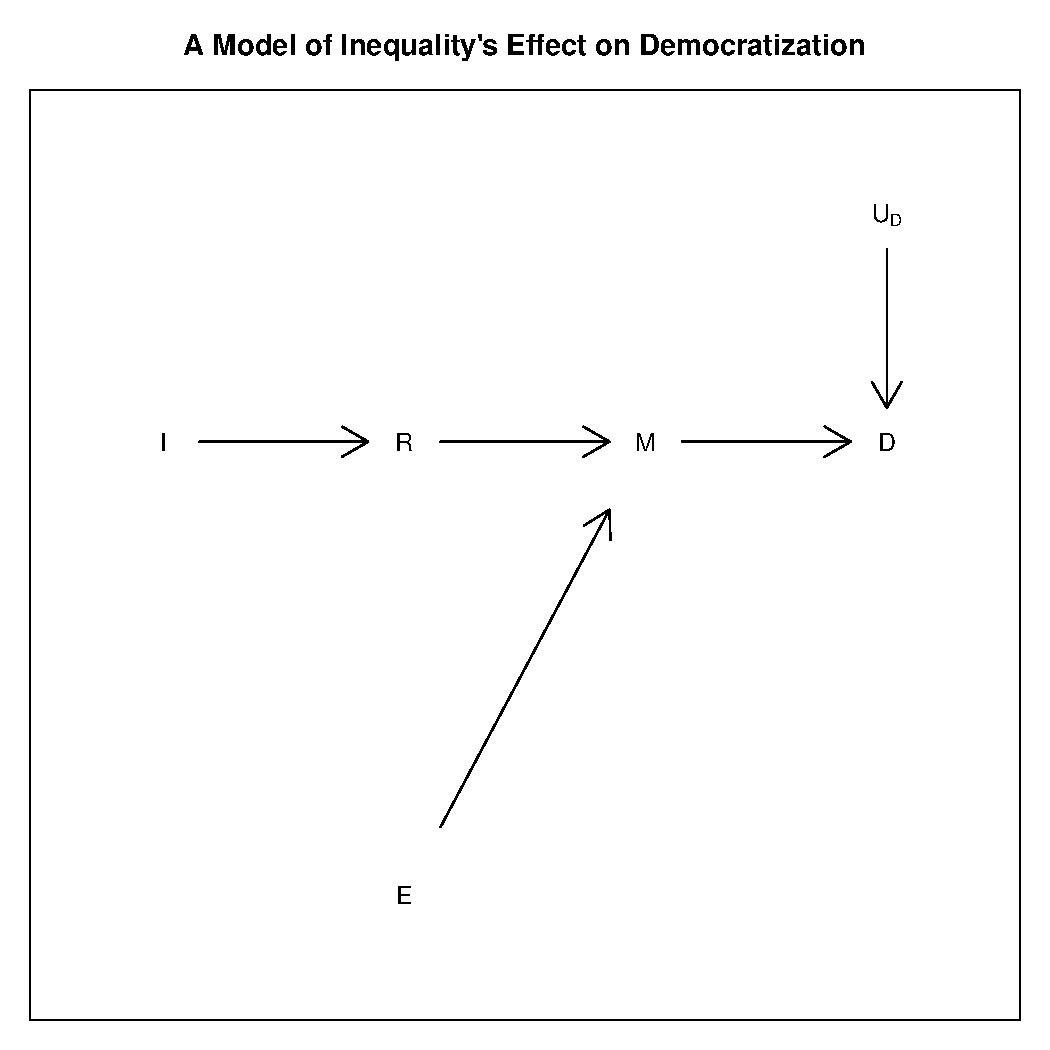
\includegraphics[width=.5\textwidth]{ii_files/figure-latex/simpleDAG-1} 

}

\caption{A simple causal model in which high inequality ($I$) affects the democratization ($D$) via redistributive demands and mass mobilization ($M$), which is also a function of ethnic homogeneity ($E$). The arrows show relations of causal dependence between variables.  The graph does not capture the ranges of the variables and the functional relations between them.}\label{fig:simpleDAG}
\end{figure}

In the context of this example, let us now consider the three components of a causal model: variables, functions, and distributions.

\textbf{The variables.} The first component of a causal model is the set of variables across which the model characterizes causal relations. On the graph in Figure \ref{fig:simpleDAG}, the 6 included variables are represented by the 6 nodes.

Notice that some of these variables have arrows pointing \emph{into} them: \(R, M\), and \(D\) are endogenous variables, meaning that their values are determined entirely by other variables in the model.

Other variables have arrows pointing out of them but no arrows pointing into them: \(I, E\) and \(U_D\) are exogenous variables. Exogenous variables are those that influence other variables in the model but themselves have no causes specified in the model. While \(I\) and \(E\) have natural interpretations, we might wonder what \(U_D\) represents as it does not feature in our substantive claims about how democratization arises. In the world of causal models, \(U\) terms are typically used to capture unspecified exogenous influences. Far from being nuisance terms, \(U\) variables constitute a key way in which we express uncertainty about the world and, in turn, are often the locus of learning about the questions we are asking. In the present example, we believe democratization to be potentially affected by mobilization, but we also know that democratization is affected by other things, even if we do not know what they are. We can thus think of \(U_D\) as a set of unknown factors---factors other than mobilization---that affect democratization.\footnote{Conventionally, we denote the set of exogenous variables as \(\mathcal{U}\) and the set of endogenous variables as \(\mathcal{V}\).}

In a causal-model framework, we sometimes use familial terms to describe relations among variables. For instance, two nodes directly connected by an arrow are known as ``parent'' and ``child,'' while two nodes with a child in common (both directly affect the same variable) are ``spouses.'' We can also say that \(I\) is an ``ancestor'' of \(D\) (a node upstream from \(D\)'s parent) and conversely that \(D\) is a descendant of \(I\) (a node downstream from \(I\)'s child).

In identifying the variables, we also need to specify the \emph{ranges} across which they can potentially vary. We might specify, for instance, that all variables in the model are binary, taking on the values 0 or 1. We could, alternatively, define a set of categories across which a variable ranges or allow a variable to take on any real number value or any value between a set of bounds. \footnote{If we let \(\mathcal{R}\) denote a set of ranges for all variables in the model, we can indicate \(X\)'s range, for instance, by writing \(\mathcal{R}(X)=\{0,1\}\). The variables in a causal model together with their ranges---the triple \((\mathcal{U}, \mathcal{V}, \mathcal{R})\)---are sometimes called a \emph{signature}, \(\mathcal{S}\).}

\textbf{The functions.} Next, we need to specify our beliefs about the causal relations among the variables in our model. How is the value of one variable affected by, and how does it affect, the values of others? For each endogenous variable---each variable influenced by others in the model---we need to express beliefs about how its value is affected by its parents, its immediate causes.

The graph already represents some aspects of these beliefs: the arrows, or directed edges, tell us which variables we believe to be direct causal inputs into other variables. So, for instance, we believe that democratization (\(D\)) is determined jointly by mobilization (\(M\)) and some exogenous, unspecified factor (or set of factors), \(U_D\). We can think of \(U_D\) as all of the other influences on democratization, besides mobilization, that we either do not know of or have decided not to explicitly include in the model. We believe, likewise, that \(M\) is determined by \(I\) and an unspecified exogenous factor (or set of factors), \(U_M\). And we are conceptualizing inequality (\(I\)) as shaped solely by a factors exogenous to the model, captured by \(U_I\). (For all intents and purposes, \(I\) behaves as an exogenous variable here since its value is determined solely by an exogenous variable.)

We can also, however, express more specific beliefs about causal relations in the form of a causal function.\footnote{The collection of all causal functions in the model can be denoted as \(\mathcal{F}\).} Specifying a function means writing down whatever general or theoretical knowledge we have about the direct causal relations between variables. A function specifies how the value that one variable takes on is determined by the values that other variables---its parents---take on.

We can specify this relationship in a vast variety of ways. Let's consider a few examples, using various variables in our running model:

\begin{itemize}
\item
  Suppose that we believe that an outcome always occurs whenever a causal condition is present. Redistributive demands, for instance, always occur whenever inequality is present. We we can express this belief with a simple function for \(R\): \(R=I\).
\item
  We can similarly express set-theoretic relations of any kind among any number of factors. We may, for instance, believe that an outcome occurs when and only when \emph{two} conditions are present. Redistributive demands and ethnic homogeneity may be individually necessary and jointly sufficient conditions for mobilization. We can express this belief with a slightly more complex function: \(M=E R\). According to this function, \(M=1\) (mobilization occurs) if \emph{both} \(E=1\) (ethnic homogeneity is present) and \(R=1\) (redistributive preferences are present), but \(M=0\) (mobilization does not occur) otherwise. Note that this formulation also builds in causal heterogeneity: here, we are saying that redistributive preferences have an effect on mobilization when and only when ethnic homogeneity is present, and vice versa.
\item
  We can model one variable as a linear function of another. Moreover, we can express uncertainty about the strength of this relationship. For instance, we can write \(R=\beta I\), where \(\beta\) is a parameter that we do not know the value of at the outset of a study (but, as we will see, may learn about from the data).
\item
  We can, further, encode uncertainty about the role of other, unknown factors in determining a variable's value. If we believe \(D\) to be linearly affected by \(M\) but also subject to forces that we do not yet understand and have not yet specified in our theory, then we can write: \(D=\beta*M+U_D\), where \(U_D\) represents a random disturbance.
\item
  We may even be uncertain about whether or in what direction one variable affects another. Or we may believe that their relationship varies across cases for reasons that we do not yet understand. We can capture this type of uncertainty as an interaction such as: \(D=M U_D\). Here, the value of our random-disturbance term does not merely represent noise around an \(M \rightarrow D\) relationship. Rather, \(U_D\) now conditions, or moderates, the strength, sign, or existence of the relationship itself. Which of these \(U_D\) conditions will depend on the \(U_D\)'s specified range. For instance, if we allow \(U_D\) to take on the values \(-1, 0\) or \(1\), then \(U_D\) will determine whether \(M\) has a negative effect, no effect, or a positive effect on \(D\). If instead, \(U_D\) is allowed to vary continuously between \(0\) and \(1\), inclusive, then it conditions the strength and existence of a positive causal effect of \(M\) on \(D\), though not the sign of that effect. As we discuss in later chapters, our investigation might then center on drawing inferences about \(U_D\) in order to assess \(M\)'s causal effect.
\item
  We can express more fundamental uncertainty about functional form, such as whether two variables are related in a linear or exponential fashion. Consider, for instance, \(D=\beta M^{U_D}\). Here, \(D\) and \(M\) are linearly related if \(U_D=1\), but exponentially if \(U_D\) is anything other than \(1\).\footnote{Here the difference between \(\beta\) and \(U_D\) is that \(\beta\) is a parameter that we believe takes a constant value for all units, even if its value is unknown, while \(U_D\) represents some unknown factor or combination of factors the value of which may vary across units, over a pre-specified range.}
\item
  Causal functions can take fully non-parametric form. Let us, for instance, allow \(U_D\) to range across the values \(a, b, c\), and \(d\). We can then write down the following causal function for \(D\):

  \begin{itemize}
  \tightlist
  \item
    if \(U_D=a\), then \(D=1-M\)
  \item
    if \(U_D=b\), then \(D=M\)
  \item
    if \(U_D=c\), then \(D=0\)
  \item
    if \(U_D=d\), then \(D=1\)
  \end{itemize}
\end{itemize}

Readers may recognize in this last causal function an expression of our original four causal types from earlier in this chapter.\footnote{The types here map directly into the four types, \(a\), \(b\), \(c\), \(d\), used in \citet{humphreys2015mixing} and into principal strata employed by Rubin and others. The literature on probabilistic models also refers to such strata as ``canonical partitions'' or ``equivalence classes.'' Note that this model is not completely general as the multinomial distribution assumes that errors are iid.} Here, \(U_D\) is an unknown factor that is conditioning the effect of mobilization on democratization, determining whether \(M\) has a negative effect, a positive effect, no effect with democratization never occurring, or no effect with democratization bound to occur regardless of mobilization.

We will make considerable use of functions similar to this last one in the pages and chapters to come. It is thus worth dwelling for a moment on what this kind of function is doing. We have started with a graph in which mobilization can have an effect on democratization and the understanding that this effect, both its existence and its sign, may vary across cases. Cases, in other words, may be of different causal types. Further, we do not know what it is that shapes \(D\)'s response to \(M\)---what makes a case one type versus another. We thus use \(U_D\) as a stand-in for the unknown and unspecified moderators of \(M\)'s effect. We might, at this stage, wonder what the point is of including \(U_D\) in the model; are we not essentially just placing a question mark on the graph? We are, and that is precisely the point. As we will see in later chapters, non-substantive, causal-type nodes can play a key role in specifying (a) what we are uncertain about in a causal network and (b) what we would like to find out. Embedding our questions about the world directly into a model of the world, in turn, allows us to answer those questions in ways systematically and transparently guided by prior knowledge.

The larger point is that functions can be written to be quite specific or extremely general, depending on the state of prior knowledge about the phenomenon under investigation. The use of a structural model \emph{does not require precise knowledge of specific causal relations}, even of the functional forms through which two variables are related.

A few important aspects of causal functions stand out. First, unlike regression equations and other equations describing data patterns, these functions express \emph{causal} beliefs. When we write \(D=\beta M\) as a function, we do not just mean that we believe the values of \(M\) and \(D\) in the world to be linearly related. We mean that we believe that the value of \(M\) \emph{determines} the value of \(D\) through this linear function. Functions are, in this sense, meant as \emph{directional} statements, with causes on the righthand side and an outcome on the left.

Second, to specify functions is to unpack a potentially complex web of causal relations into its constituent causal links. For each variable, we do not need to think through entire sequences of causation that might precede it. We need only specify how we believe it to be affected by its parents---that is to say, those variables pointing directly into it. Our outcome of interest, \(D\), may be a shaped by multiple, long chains of causality. To theorize how \(D\) is generated, however, we write down how we believe \(D\) is shaped by its immediate causes, \(M\) and \(U_D\). We then, separately, express a belief about how \(M\) is shaped by \emph{its} direct causes, \(R\) and \(E\). A variable's function must include as inputs all, and only, those variables that point directly into that variable.\footnote{The set of a variable's parents is required to be minimal in the sense that a variable is not included among the parents if, given the other parents, the child does not depend on it in any state that arises with positive probability.}

Third, as in the general potential-outcomes framework, all relations in a causal model are conceptualized as in principle deterministic: a variable's value is fully \emph{determined} by the values of its parents---i.e., by the righthand side terms in its functional equation. We express uncertainty about causal relations, however, either as unknown paramaters (e.g., \(\beta\), above) or as random disturbances, the \(U\) terms.

Fourth and relatedly, in a properly specified causal model \emph{the values of the exogenous variables}---those with no arrows pointing in to them---\emph{are sufficient to determine the values of all other variables in the model.} Consistent with more informal usage, we refer to a given set of values for all exogenous terms in a model as a \emph{context}. In causal model, context determines all other values. For instance, in Figure \ref{fig:simpleDAG}, knowing the values of \(I\), \(E\), and \(U_D\) as well as the causal functions (including the values of any parameters they contain) would tell us the values of \(R\), \(M\), and \(D\).

\textbf{The distributions.} Putting these components together gives what is termed a \emph{structural causal model.} In a structural causal model, all endogenous variables are, either directly or by implication, functions of a case's context (the values of the set of exogenous variables).\footnote{More formally, a \textbf{structural causal model} \emph{over} signature \(\mathcal{S}=<\mathcal{U},\mathcal{V},\mathcal{R}>\) is a pair \(<\mathcal{S}, \mathcal{F}>\), where \(\mathcal{F}\) is a set of ordered structural equations containing a function \(f_i\) for each element \(Y\in \mathcal{V}\). We say that \(\mathcal{F}\) is a set of ordered structural equations if no variable is its own descendant and if no element in \(\mathcal{U}\) is parent to more than one element of \(\mathcal{V}\). This last condition can be achieved by shifting any parent of multiple children in \(\mathcal{U}\) to \(\mathcal{V}\). This definition thus includes an assumption of acyclicity, which is not found in all definitions in the literature.} What we have not yet inscribed into the model, however, is any beliefs about how \emph{likely} or \emph{common} different kinds of contexts might be. Thus, for instance, a structural causal model consistent with Figure \ref{fig:simpleDAG} stipulates that \(I\), \(E\), and \(U_D\) may have effects on \(D\), but it says nothing in itself about the distribution of \(I\), \(E\), and \(U_D\) themselves, beyond limitations on their ranges.\footnote{Thus \(P(d|i,e, u_D)\) would defined by this structural model (as a degenerate distribution), but \(P(i)\), \(P(e)\), \(P(u_D)\), and \(P(i,e, u_D)\) would not be.} We have not said anything, for instance, about how common high inequality is across the relevant domain of cases, how common ethnic homogeneity is, or how unspecified inputs are distributed.

In many research situations, we will have beliefs not just about how the world works under different conditions, but also about what kinds of conditions are more likely than others. We can express these beliefs about context as probability distributions over the models exogenous terms.\footnote{We assume that the exogenous terms, the elements of \(\mathcal{U}\), are generated independently of one another. While this is not without loss of generality, it is not as constraining as it might at first appear: any graph in which two exogenous variables are not independent can be replaced by a graph in which these two terms are listed as endogenous (possibly unobserved) nodes, themselves generated by a third variable. Note also that one could envision ``incomplete probabilistic causal models'' in which researchers claim knowledge regarding distributions over \emph{subsets} of \(\mathcal{U}\).} For instance, a structural causal model might support a claim of the form: ``\(R\) has a positive effect on \(M\) if and only if \(E=1\) holds.'' We might, then, add to this a belief that \(E=1\) in 25\% of cases in the population of interest. Including this belief about context implies, in turn, that \(R\) has a positive effect on \(M\) a quarter of the time. As with the functions, we can also (and typically would) build uncertainty into this belief by specifying a \emph{distribution} over possible shares of cases with ethnic homogeneity, with our degree of uncertainty captured by the distribution's variance.

\begin{center}\rule{0.5\linewidth}{\linethickness}\end{center}

Technical Note on the Markov Property
The assumptions that no variable is its own descendant and that the \(U\) terms are generated independently make the model \emph{Markovian}, and the parents of a given variable are Markovian parents. Knowing the set of Markovian parents allows one to write relatively simple factorizations of a joint probability distribution, exploiting the fact (``the Markov condition'') that all nodes are \emph{conditionally independent} of their nondescendants, conditional on their parents. Variables \(A\) and \(B\) are ``conditionally independent'' given \(C\) if \(P(a|b,c) = P(a|c)\) for all values of \(a, b\) and \(c\).\\
To see how this Markovian property allows for simple factorization of \(P\) for Figure \ref{fig:simpleDAG}, note that \(P(X, R, Y)\) can always be written as:
\[P(X, R, Y) = P(X)P(R|X)P(Y|R, X)\]
If we believe, as in the figure, that \(X\) causes \(Y\) only through \(R\) then we have the slightly simpler factorization:
\[P(X, R, Y) = P(X)P(R|X)P(Y|R)\]
Or, more generally:

\begin{equation} 
P(v_1,v_2,\dots v_n) = \prod P(v_i|pa_i)
\label{eq:markov}
\end{equation}

The distribution \(P\) on \(\mathcal{U}\) induces a joint probability distribution on \(\mathcal{V}\) that captures not just information about how likely different states are to arise but also the relations of conditional independence between variables that are implied by the underlying causal process. For example, if we thought that \(X\) caused \(Y\) via \(R\) (and only via \(R\)), we would then hold that \(P(Y | R) = P(Y | X, R)\): in other words if \(X\) matters for \(Y\) only via \(R\) then, conditional on \(R\), \(X\) should not be informative about \(Y\).\\
In this way, a probability distribution \(P\) over a set of variables can be consistent with some causal models but not others. This does not, however, mean that a specific causal model can be extracted from \(P\). To demonstrate with a simple example for two variables, any probability distribution on \((X,Y)\) with \(P(x)\neq P(x|y)\) is consistent both with a model in which \(X\) is a parent of \(Y\) and with a model in which \(Y\) is a parent of \(X\).

\begin{center}\rule{0.5\linewidth}{\linethickness}\end{center}

Once we introduce beliefs about the distribution of values of the exogenous terms in a model, we have specified a \emph{probabilistic causal model.} We need not say much more, for the moment, about the probabilistic components of causal models. But to foreshadow the argument to come, our prior beliefs about the likelihoods of different contexts play a central role in the framework that we present in this book. We will see how the encoding contextual knowledge---beliefs that some kinds of conditions are more common than others---forms a key foundation for causal inference. At the same time, our expressions of \emph{uncertainty} about context represent scope for learning: it is the very things that we are, at a study's outset, uncertain about that we can update our beliefs about as we encounter evidence.

\hypertarget{features-of-causal-models}{%
\subsection{Features of causal models}\label{features-of-causal-models}}

The diagram in Figure \ref{fig:simpleDAG} is called a causal graph. Though we have already been making use of this causal graph to help us visualize elements of a causal model, we now explicitly point out a number of general features of causal graphs as we will be using them throughout this book. Causal graphs have their own distinctive ``grammar,'' a set of rules that give them important analytical features.

A causal graph represents elements of a causal model as a set of nodes (or vertices), representing variables, connected by a collection of single-headed arrows (or directed edges). We draw an arrow from node \(A\) to node \(B\) if and only if we believe that \(A\) can have a direct effect on \(B\). The resulting diagram is a \emph{directed acyclic} graph (DAG) if there are no paths along directed edges that lead from any node back to itself---i.e., if the graph contains no causal cycles.

The drawing of causal graphs follows two rules. \footnote{These two conditions define a `'causal DAG'' \citep{hernan2006instruments}. Further, the specification that \(\mathcal{F}\) is a set of ordered structural equations ensures that the graph is acyclic.} First, the \emph{absence} of an arrow between \(A\) and \(B\) means that \(A\) is not a direct cause of \(B\).\footnote{By ``direct'' we mean that the \(A\) is a parent of \(B\): i.e., the effect of \(A\) on \(B\) is not fully mediated by one or more other variables in the model.} Here lies an important asymmetry: drawing such an arrow does not mean that we know that \(A\) \emph{does} directly cause \(B\); but omitting such an arrow implies that we know that \(A\) does \emph{not} directly cause \(B\). We say more, in other words, with the arrows we omit than with the arrows that we include.

Returning to Figure \ref{fig:simpleDAG}, we have here expressed the belief that redistributive preferences exert no direct effect on democratization; we have done so by \emph{not} drawing an arrow directly from \(R\) to \(D\). In the context of this model, saying that redistributive preferences have no direct effect on democratization is to say that any effect of redistributive preferences on democratization \emph{must} run through mobilization; there is no other pathway through which such an effect can operate. This might be a way of encoding the knowledge that mass preferences for redistribution cannot induce autocratic elites to liberalize the regime absent collective action in pursuit of those preferences.

The same goes for the effects of \(I\) on \(M\), \(I\) on \(D\), and \(E\) on \(D\): the graph in Figure \ref{fig:simpleDAG} implies that we believe that these effects also do not operate directly, but only along the indicated, mediated paths.

Meanwhile, the existence of an arrow from \(A\) to \(B\) does not imply that \(A\) always, or even ever, has a direct effect on \(B\). Consider, for instance, the arrow running from \(R\) to \(M\). The existence of this arrow requires that \(M\) appear somewhere in the \(M\)'s functional equation as a variable's functional equation must include all variables pointing directly into it. Imagine, though, that \(M\)'s causal function is specified as: \(M = RE\). This function allows for the \emph{possibility} that \(R\) affects \(M\), as it will whenever \(E=1\). However, it also allows that \(R\) will have no effect, as it will when \(E=0\).

This example also, incidentally, demonstrates another important consequence of context, the values of the exogenous variables: a case's context determines not just the settings on the endogenous variables, but also the causal \emph{effects} that prevail among the variables. Under the functional equation \(M=RE\), a case's ethnic-compositional context determines whether or not redistributive preferences will have an effect on mobilization.

The second rule of drawing DAGs is that any cause common to multiple variables on the graph must itself be represented on the graph. If \(A\) and \(B\) on a graph are both affected by some third variable, \(C\), then we must represent this common cause. Put differently, any two variables without common causes on the graph are taken to be indepedent of one another. Thus, the graph in Figure \ref{fig:simpleDAG} implies that the values of \(I\), \(E\), and \(U_D\) are all determined independently of one another. If in fact we believed that a country's level of inequality and its ethnic composition were both shaped by, say, its colonial heritage, then this DAG would \emph{not} be an accurate representation of our beliefs about the world. To make it accurate, we would need to add to the graph a variable capturing that colonial heritage and include arrows running from colonial heritage to both \(I\) and \(E\).

This rule ensures that the graph captures all potential correlations among variables that are implied by our beliefs. If \(I\) and \(E\) are in fact driven by some common cause, then this means not just that these two variables will be correlated but also that each will be correlated with any consequences of the other. For instance, a common cause of \(I\) and \(E\) would also imply a correlation between \(R\) and \(E\). \(R\) and \(E\) are implied to be independent in the current graph but would be implied to be correlated if a common node pointed into both \(I\) and \(E\).

Of particular interest in Figure \ref{fig:simpleDAG} is the implied independence of \(U_D\) from every other node. Imagine, for instance, an additional node pointing into both \(I\) and \(U_D\). This would represent a classic form of confounding: the assignment of cases to values on the explanatory variable would be correlated with case's potential outcomes on \(D\). The omission of any such pathway is precisely equivalent to expressing the belief that \(I\) is exogenous, or (as if) randomly assigned.

The flip side of this second rule is that a causal graph, to do the work it must do, does \emph{not} need to include everything we know about a substantive domain of interest. We may know quite a lot about the causes of economic inequality, for example. But we can safely omit these other factors from the graph as long as they do not have effects on other variables in the graph (via some path that does not run through \(I\)). Likewise, we can choose to capture any number of unspecified factors in a \(U\) term. We may be aware of a vast range of forces shaping whether countries democratize, but choose to bracket them for the purposes of an examination of the role of economic inequality. The \(U_D\) achieves this bracketing and is permissble as long as none of these unspecified factors also act on the other variables included in the model (since, if they do, then we would have a common cause of two included variables and would then need to capture the implied correlation between them).

Moreover, as a matter of convention, explicitly including \(U\) terms is optional. In practice, \(U\)'s are often excluded from the visual representation of a model on the understanding that every variable on the graph is subject to some unaccounted-for influence and thus, implicitly, has a \(U\) term pointing into it. In this book, we will generally draw the \(U\) terms where they are of particular theoretical or analytical interest but will otherwise omit them. Whether we include or omit \(U\) terms, we will generally treat those nodes in a graph that have no arrows pointing into them as the exogenous variables that define the context.

As should be clear, a DAG does not represent all features of a causal model. What it does record is which variables enter into the structural equation for every other variable: what can directly cause what. But the DAG contains no other information about the form of those causal relations. Thus, for instance, the DAG in Figure \ref{fig:simpleDAG} tells us that \(M\) is function of both \(R\) and \(E\), but it does not tell us whether that joint effect is additive (\(R\) and \(E\) separately increase mobilization), interactive (the effect of each depends on the value of the other), or whether either effect if linear, curvilinear or something else.

This lack of information about functional forms often puzzles those encountering causal graphs for the first time; surely it would be convenient to visually differentiate, say, additive from conditioning effects. As one thinks about the variety of possible causal functions, it quickly becomes clear that there would be no simple visual way of capturing all possible functional relations. Moreover, as we shall now see, causal graphs are a tool designed with a particular analytic purpose in mind---a purpose to which we now turn.

\hypertarget{conditional-independence-from-dags}{%
\subsection{Conditional independence from DAGs}\label{conditional-independence-from-dags}}

If we encode our prior knowledge using the grammar of a causal graph, we can put that knowledge to work for us in powerful ways. In particular, the rules of DAG-construction allow for an easy reading of the \emph{conditional independencies} implied by our beliefs.

To begin thinking about conditional independence, it can be helpful to conceptualize dependencies between variables as generating \emph{flows of information}. Let us first consider a simple relationship of dependence. Returning to Figure \ref{fig:simpleDAG}, the arrow running from \(I\) to \(R\), implying a direct causal dependency, means that if we expect \(I\) and \(R\) to be correlated. Put differently, observing the value of one of these variables also gives us information about the value of the other. If we measured redistributive preferences, the graph implies that we would also be in a better position to infer the level of inequality, and vice versa. Likewise, \(I\) and \(M\) are also linked in a relationship of dependence: since inequality can affect mobilization (through \(R\)), knowing the the level of inequality would allow us to improve our estimate of the level of mobilization and vice versa.

In contrast, consider \(I\) and \(E\), which are in this graph indicated as being \emph{independent} of one another. Learning the level of inequality, according to this graph, would give us no information whatsoever about the degree of ethnic homogeneity, and vice-versa.

Moreover, sometimes what you learn depends on \emph{what you already know.} Suppose that we already knew the level of redistributive preferences. Would we then be in a position to learn about the level of inequality by observing the level of mobilization? According to this graph we would not: since the causal link---and, hence, flow of information between \(I\) and \(M\)---runs through \(R\), and we already know \(R\), there is nothing left to be learned about \(I\) by also observing \(M\). Anything we could have learned about inequality by observing mobilization is already captured by the level of redistributive preferences, which we have already seen. While \(I\) and \(M\) are dependent---one is informative about the other---if we have \emph{not} seen \(R\), they are independent of one another (uninformative about each other) if we have seen \(R\). We can express this idea by saying that \(I\) and \(M\) are \emph{conditionally independent given \(R\)}.

We say that two variables, \(A\) and \(C\), are ``conditionally independent'' given a set of variables \(\mathcal B\) if, once we have knowledge of the values in \(\mathcal B\), knowledge of \(A\) provides no information about \(C\) and vice-versa. Taking \(\mathcal B\) into account thus ``breaks'' any relationship that might exist unconditionally between \(A\) and \(C\).

To take up another example, suppose that war is a cause of both military casualties and price inflation, as depicted in Figure \ref{fig:warDAG}. Casualties and inflation will then be (unconditionally) correlated with one another because of their shared cause. If I learn that there have been military casualties, this information will lead me to think it more likely that there is also war and, in turn, price inflation (and vice versa). However, assuming that war is their only common cause, we would say that military casualties and price inflation are \emph{conditionally independent given war.} If we already know that there is war, then we can learn nothing further about the level of casualties (price inflation) by learning about price inflation (casualties). We can think of war, when observed, as blocking the flow of information between its two consequences; everything we would learn about inflation from casualties is already contained in the observation that there is war. Put differently, if we were just to look at cases where war is present (i.e., if we hold war constant), we should find no correlation between military casualties and price inflation; likewise, for cases in which war is absent.

\begin{figure}

{\centering 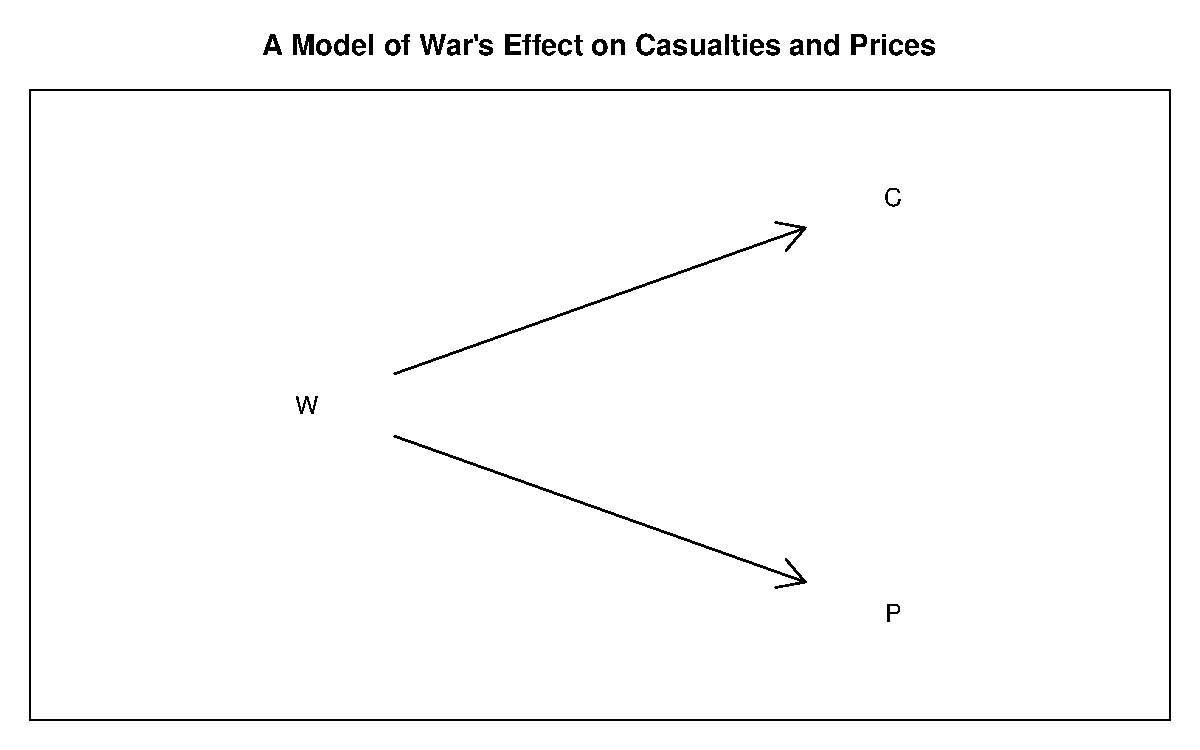
\includegraphics[width=.5\textwidth]{ii_files/figure-latex/warDAG-1} 

}

\caption{This graph represents a simple causal model in which war ($W$) affects both military casualties ($C$) and price inflation ($P$).}\label{fig:warDAG}
\end{figure}

Relations of conditional independence are central to the strategy of statistical control, or covariate adjustment, in correlation-based forms of causal inference, such as regression. In a regression framework, identifying the causal effect of an explanatory variable, \(X\), on a dependent variable, \(Y\), requires the assumption that \(X\)'s value is conditionally independent of \(Y\)'s potential outcomes (over values of \(X\)) given the model's covariates. To draw a causal inference from a regression coefficient, in other words, we have to believe that including the covariates in the model ``breaks'' any biasing correlation between the value of the causal variable and its unit-level effect.

As we will explore, however, relations of conditional independence are of more general interest in that they tell us, given a model, \emph{when information about one feature of the world may be informative about another feature of the world, given what we already know}. By identifying the possibilities for learning, relations of conditional independence can thus guide research design.

To see more systematically ow a DAG can reveal conditional independencies, it is useful spell out three pairs of features of the flow of information in causal graphs:

\begin{figure}

{\centering 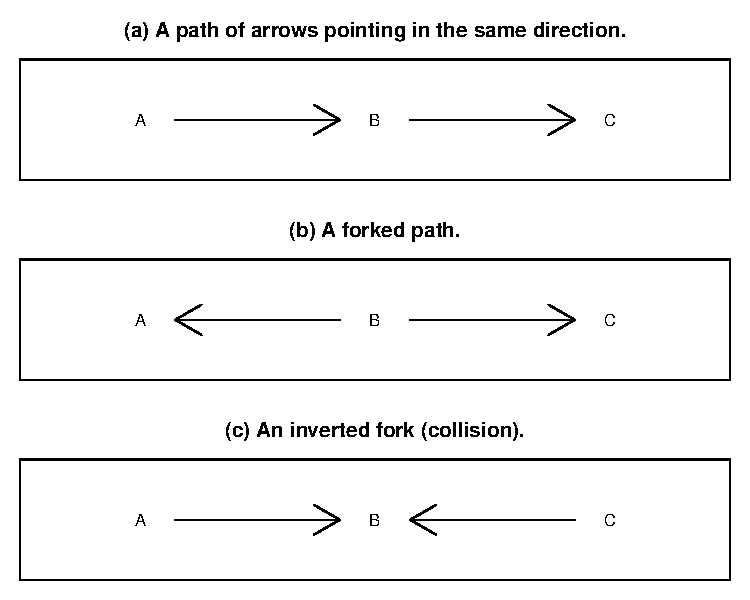
\includegraphics[width=.9\textwidth]{ii_files/figure-latex/unnamed-chunk-6-1} 

}

\caption{\label{fig:CI} Three elementary relations of conditional independence.}\label{fig:unnamed-chunk-6}
\end{figure}

(1a) Information can flow unconditionally along a path of arrows pointing in the same direction. In Panel 1 of Figure \ref{fig:CI}, information flows across all three nodes. Learning about any one will tell us something about the other two.

(1b) Learning the value of a variable along a path of arrows pointing in the same direction \emph{blocks} flows of information across that variable. Knowing the value of \(B\) in Panel 1 renders \(A\) no longer informative about \(C\), and vice versa: anything that \(A\) might tell us about \(C\) is already captured by the information about \(B\).

(2a) Information can flow unconditionally across the branches of any forked path. In Panel 2 learning only \(A\) can provide information about \(C\) and vice-versa.

(2b) Learning the value of the variable at the forking point blocks \emph{flows} of information across the branches of a forked path. In Panel 2, learning \(A\) provides no information about \(C\) if we already know the value of \(B\).\footnote{Readers may recognize this statement as the logic of adjusting for a confound that is a cause of both an explanatory variable and a dependent variable in order to achieve conditional independence.}

(3a) When two or more arrowheads collide, generating an inverted fork, there is no unconditional flow of information between the incoming sequences of arrows. In Panel 3, learning only \(A\) provides no information about \(C\), and vice-versa.

(3b) Collisions can be sites of \emph{conditional} flows of information. In the jargon of causal graphs, \(B\) in Panel 2 is a ``collider'' for \(A\) and \(C\).\footnote{In the familial language of causal models, a collider is a child of two or more parents.} Although information does not flow unconditionally across colliding sequences, it does flow across them \emph{conditional} on knowing the value of the collider variable or any of its downstream consequences. In Panel 2, learning \(A\) \emph{does} provide new information about \(C\), and vice-versa, \emph{if} we also know the value of \(B\) (or, in principle, the value of anything that \(B\) causes).

The last point is somewhat counter-intuitive and warrants further discussion. It is easy enough to see that, for two variables that are correlated unconditionally, that correlation can be ``broken'' by controlling for a third variable. In the case of collision, two variables that are \emph{not} correlated when taken by themselves \emph{become} correlated when we condition on (i.e., learn the value of) a third variable, the collider. The reason is in fact quite straightforward once one sees it: if an outcome is a joint function of two inputs, then if we know the outcome, information about one of the inputs can provide information about the other input. For example, if I know that you have brown eyes, then learning that your mother has blue eyes makes me more confident that your father has brown eyes.

Looking back at our democratization DAG in Figure \ref{fig:simpleDAG}, \(M\) is a collider for \(R\) and \(E\), its two inputs. Suppose that we again have the functional equation \(M=RE\). Knowing about redistributive preferences alone provides no information whatsoever about ethnic homogeneity since the two are determined independently of one another. On the other hand, imagine that you already know that there was no mobilization. Now, if you observe that there \emph{were} redistributive preferences, you can figure out the level of ethnic homogeneity: it must be 0. (And likewise in going from homogeneity to preferences.)

Using these basic principles, conditional independencies can be read off any DAG. We do so by checking every path connecting two variables of interest and ask whether, along those paths, the flow of information is open or blocked, given any other variables whose values are already observed. Conditional independence is established when \emph{all} paths are blocked given what we already know; otherwise, conditional independence is absent.

As an exercise, see whether you can identify the relations of conditional independence between \(A\) and \(D\) in Figure \ref{fig:CItest}.

\begin{figure}

{\centering 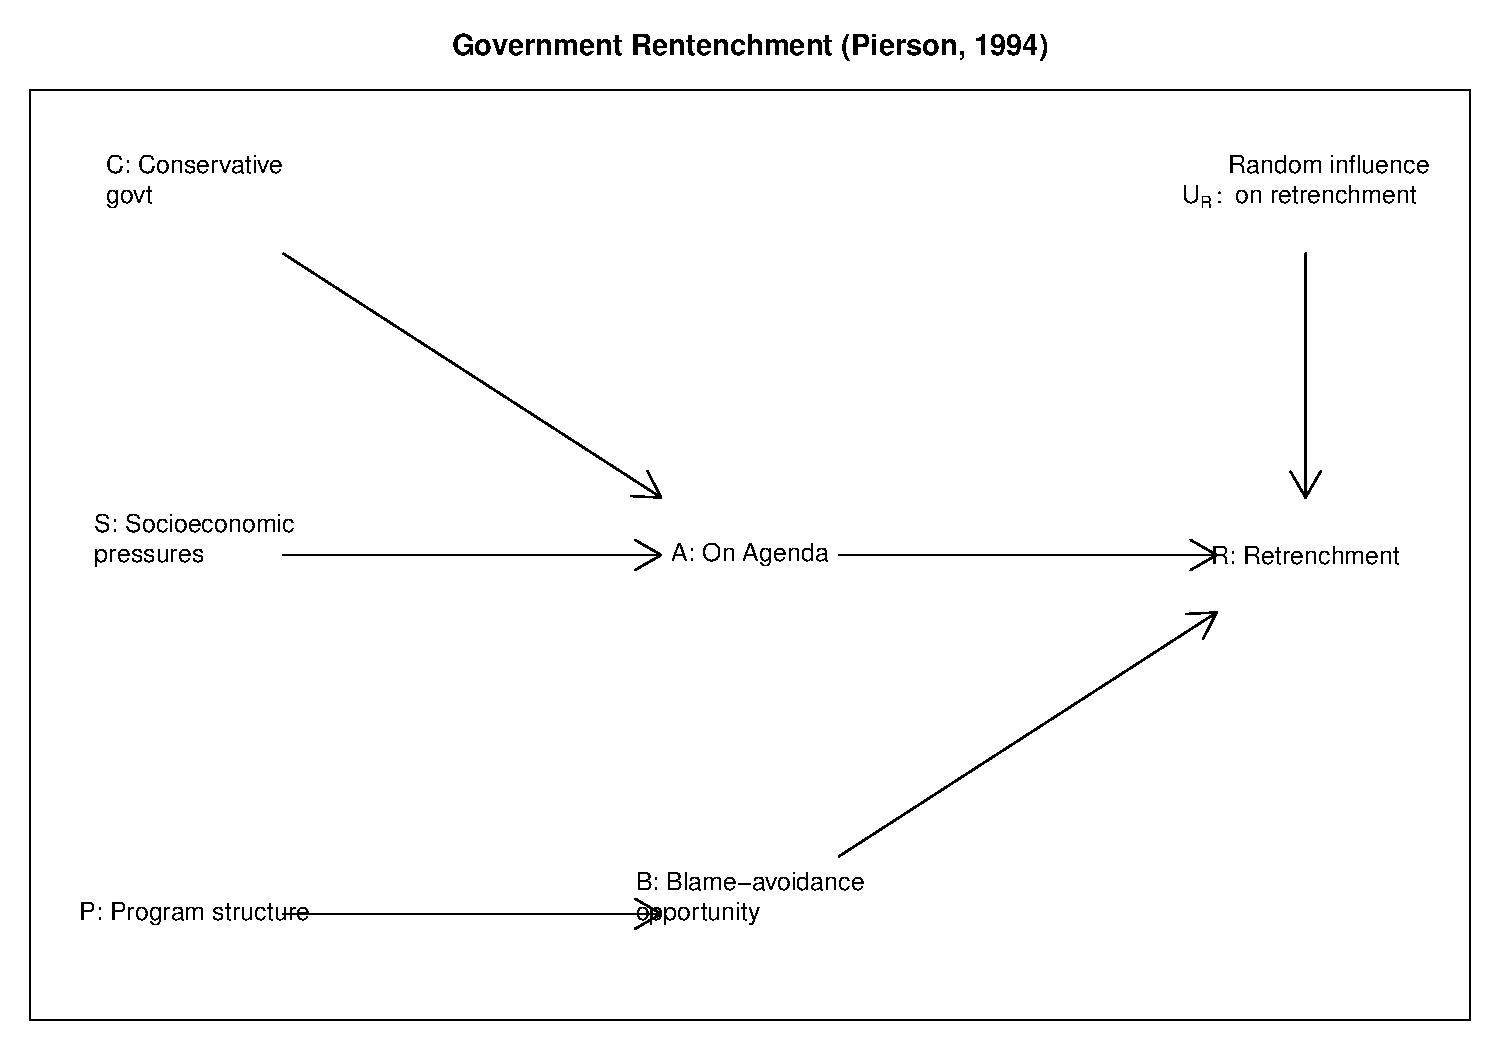
\includegraphics[width=.9\textwidth]{ii_files/figure-latex/unnamed-chunk-7-1} 

}

\caption{\label{fig:CItest} An exercise: $A$ and $D$ are conditionally independent, given which other variable(s)?}\label{fig:unnamed-chunk-7}
\end{figure}

Are A and D independent:

\begin{itemize}
\tightlist
\item
  unconditionally?
\end{itemize}

Yes. \(B\) is a collider, and information does not flow across a collider if the value of the collider variable or its consequences is not known. Since no information can flow between \(A\) and \(C\), no information can flow between \(A\) and \(D\) simply because any such flow would have to run through \(C\).

\begin{itemize}
\tightlist
\item
  if you condition on \(B\)?
\end{itemize}

No.~Conditioning on a collider opens the flow of information across the incoming paths. Now, information flows between \(A\) and \(C\). And since information flows between \(C\) and \(D\), \(A\) and \(D\) are now also connected by an unbroken path. While \(A\) abnd \(D\) were independent when we conditioned on nothing, they cease to be independent when we condition on \(B\).

\begin{itemize}
\tightlist
\item
  if you condition on \(C\)?
\end{itemize}

Yes. Conditioning on \(C\), in fact, has no effect on the situation. Doing so cuts off \(B\) from \(D\), but this is irrelevant to the \(A\)-\(D\) relationship since the flow between \(A\) and \(D\) was already blocked at \(B\), an unobserved collider.

\begin{itemize}
\tightlist
\item
  if you condition on \(B\) and \(C\)?
\end{itemize}

Yes. Now we are doing two, countervailing things at once. While conditioning on \(B\) opens the path connecting \(A\) and \(D\), conditioning on \(C\) closes it again, leaving \(A\) and \(D\) conditionally independent.

Analyzing a causal graph for relations of independence represents one payoff to formally encoding our beliefs about the world in a causal model. We are, in essence, drawing out implications of those beliefs: given what we believe about a set of direct causal relations (the arrows on the graph), what must this logically imply about other dependencies and independencies on the graph, conditional on having observed some particular set of nodes? We show in a later chapter how these implications can be deployed to guide research design, by indicating which parts of a causal system are potentially informative about other parts that may be of interest.

\hypertarget{a-simple-running-example}{%
\subsection{A simple running example}\label{a-simple-running-example}}

We will illistrate these core ideas with a simple running example of a model of government corruption and survival.

We begin with two binary features of context. Consider, first, that a country may or may not have a free press (\(X\)). Second, the country's government may or may not be sensitive to public opinion (\(S\)).\footnote{Government sensitivity here can be thought of as government sophistication (does it take the actions of others into account when making decisions?) or as a matter of preferences (does it have a dominant strategy to engage in corruption?).} Let us then stipulate what follows from these conditions. The government will engage in corruption (\(C=1\)) unless it is sensitive to public opinion and there is a free press. Moreover, if and only if there is both government corruption and a free press, the press will report on the corruption (\(R=1\)). Finally, the government will be removed from office (\(Y=1\)) if it has acted corruptly and this gets reported in the press; otherwise, the government remains in office.

As a set of equations, this simple causal model may be written as follows:

\(\begin{array}{ll} C = 1-X\times S & \mbox{Whether the government is corrupt}\\ R = C\times X & \mbox{Whether the press reports on corruption}\\ Y = C\times R & \mbox{Whether the government is removed from office} \end{array}\)

One thing that these equations make clear is that the variables in our model function in various places as causal-type nodes for one another. For instance, we can see from equation for \(C\) that the causal effect of a free press (\(X\)) on corruption (\(C\)) depends on whether the government is sensitive to public opinion (\(S\)): \(S\) determines \(C\)'s response to \(X\) (as does \(X\) for \(S\)'s effect on \(C\)). A similar relationship holds for \(C\) and \(X\) in their effect on \(R\) and for \(C\) and \(R\) in their effect on \(Y\). As we will see below, the model also implies more complex causal-type relationships. We can, further, substitute through the causal processes to write down the functional equation for the outcome in terms of the two initial causal variables: \(Y=(1-S)X\).\footnote{Equivalently, in Boolean terms, where \(Y\) stands for the occurrence of government removal, \(Y= \neg S \land X\); and the function for the outcome ``government retained'' can be written \(\neg Y = (S\land X) \lor (S\land\neg X) \lor (\neg S \land \neg X)\) or, equivalently, \(\neg Y = S + \neg S \neg X\).}

Let us, further, allow our two primary causal variables---the existence of a free press and the existence of a sensitive government---to vary probabilistically. In particular, we represent the probability of a free press with the population parameter \(\lambda^X_1\) and the probability of a sensitive government with the parameter \(\lambda^S_1\). To generate draws based on these probabilities, we then introduce two random variables with uniform distributions between 0 and 1, \(U_X\) and \(U_S\), and posit that we get a free press, \(\theta^X=\theta^X_1\) whenever \(u_X < \lambda^X_1\) and a sensitive government, \(\theta^S=\theta^S_1\), whenever \(u_S < \lambda_1^S\).

This gives the following equations for \(X\) and \(S\):

\(\begin{array}{ll} X = \mathbb{1}(u_X < \lambda^X_1) & \mbox{Whether the press is free}\\ S = \mathbb{1}(u_S < \lambda^S_1) & \mbox{Whether the government is sensitive}\\ \end{array}\)

Note that in this model, only the most ``senior'' specified variables, \(X\) and \(S\), have a stochastic component (i.e., \(\lambda^X_1\) and \(\lambda^S_1\) lie between 0 and 1). All other endogenous variables are deterministic functions of other specified variables.

\begin{figure}

{\centering 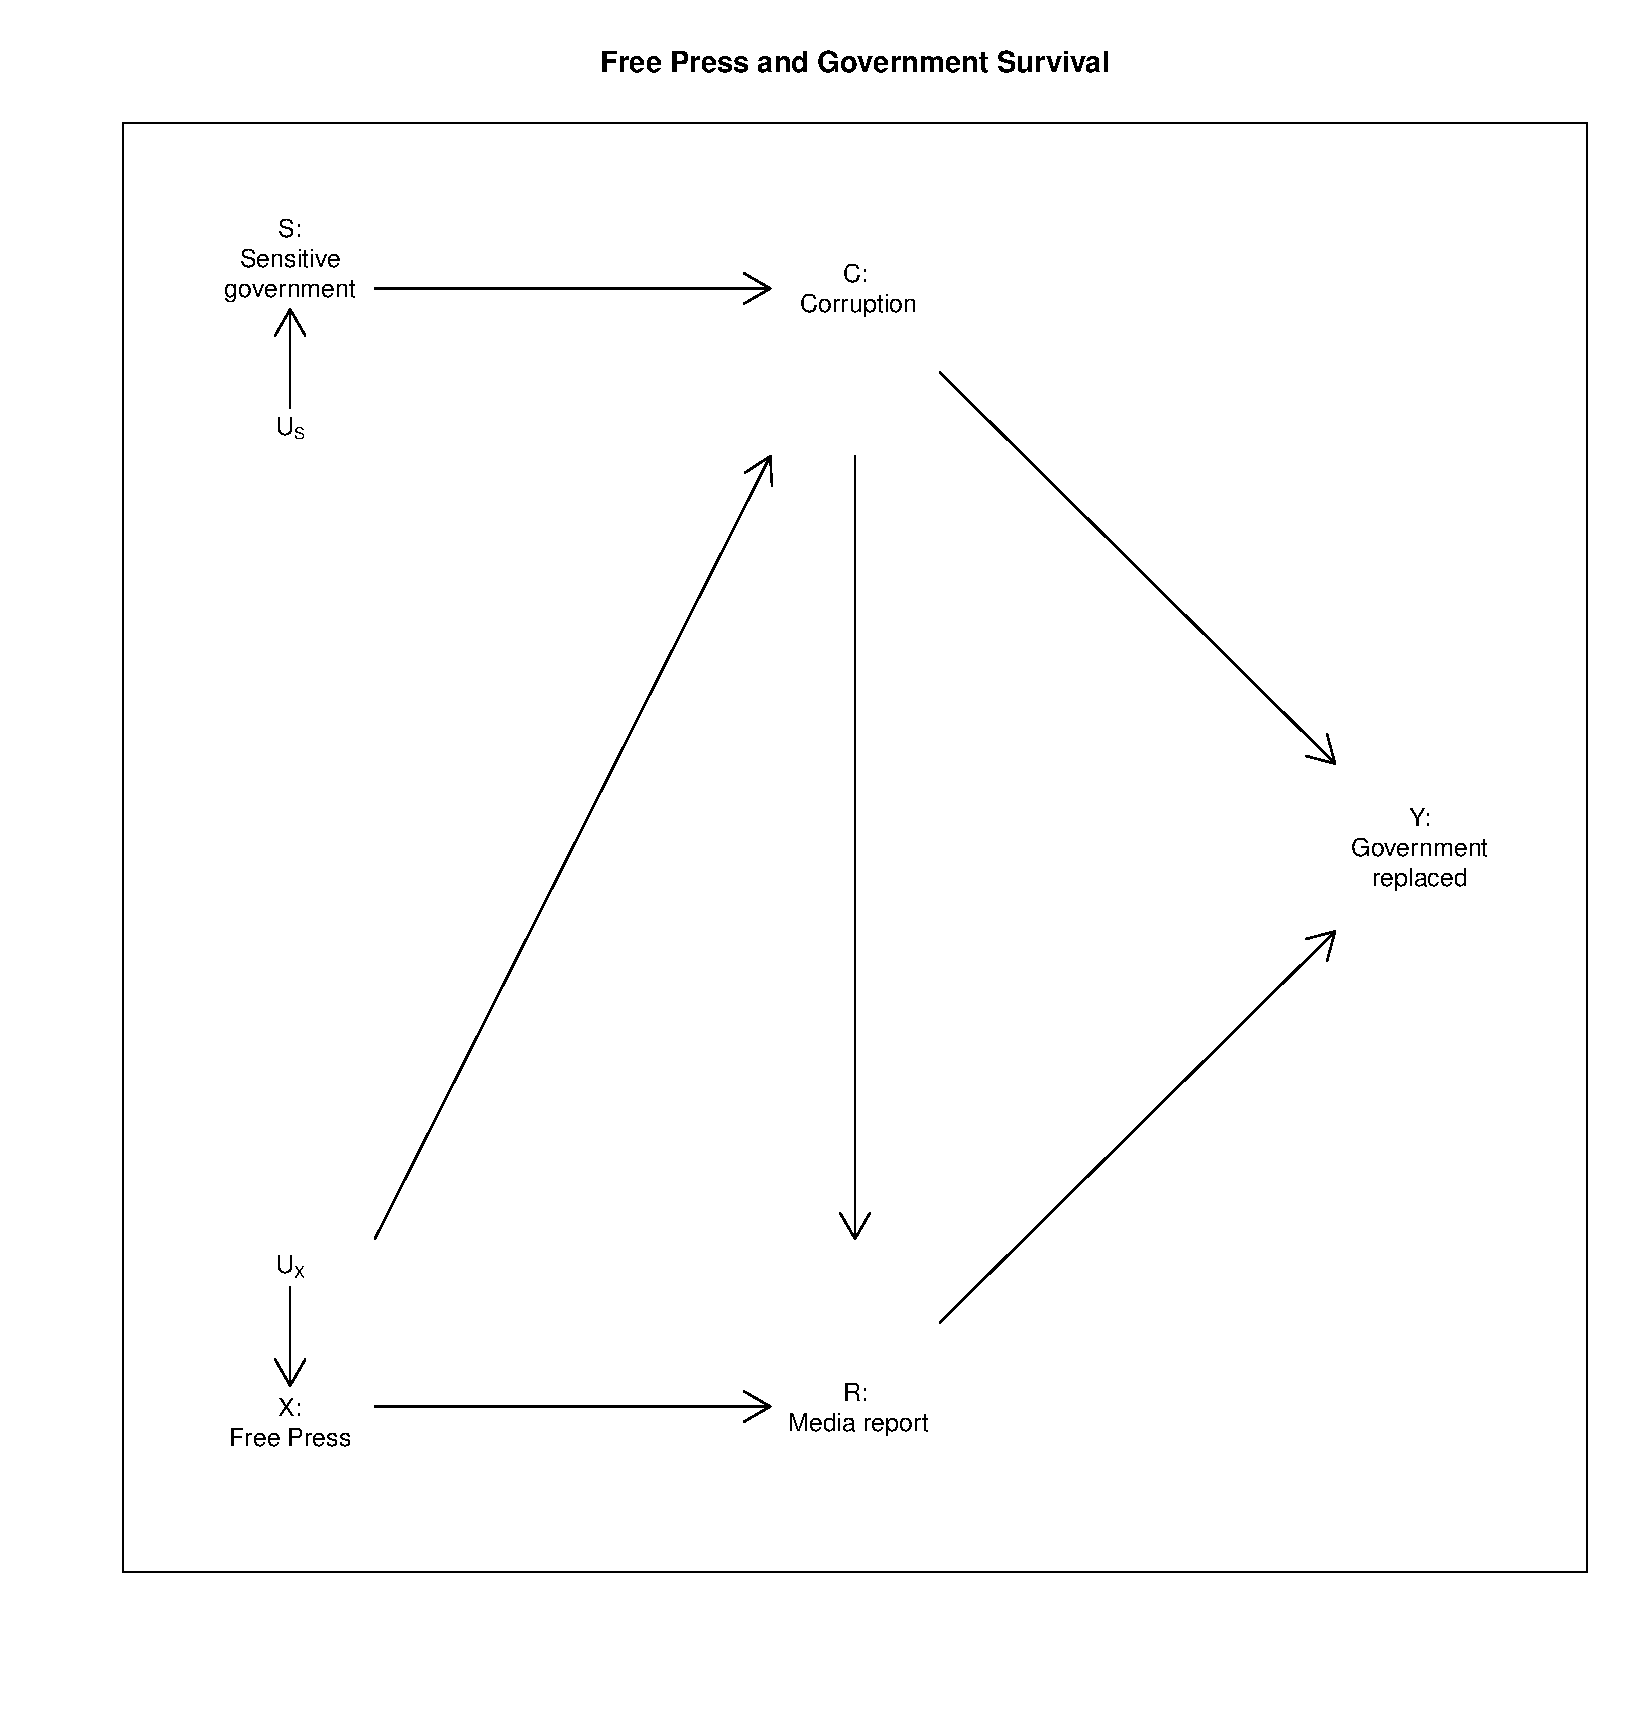
\includegraphics[width=\textwidth]{ii_files/figure-latex/running-1} 

}

\caption{The figure shows a simple causal model. $S$ and $X$ are stochastic, other variables determined by their parents, as shown in bottom right panel.}\label{fig:running}
\end{figure}

The corresponding causal diagram for this model is shown in Figure \ref{fig:running}. The graph explicitly includes the processes determining the two key causal variables variables (the \(\lambda\) and \(U\) terms).

\hypertarget{causal-models-from-the-literature}{%
\section{Causal models from the literature}\label{causal-models-from-the-literature}}

We can provide more of a sense of how one might encode prior knowledge in a causal model by asking how we might construct models in light of extant scholarly works. We undertake this exercise here for three well-known works in comparative politics and international relations: Pierson's seminal book on welfare-state retrenchment (\citet{pierson1994dismantling}); Elizabeth Saunders' research on leaders' choice of military intervention strategies (\citet{saunders2011leaders}); and Przeworski and Limongi's work on democratic survival (\citet{przeworski1997modernization}), an instructive counterpoint to Boix's (\citet{boix2003democracy}) argument about a related dependent variable. For each, we represent in the form of a causal model the causal knowledge that we might plausibly think we take away from the work in question. Readers might represent these knowledge bases differently; our present aim is merely to illustrate how causal models are constructed, rather than to defend a particular representation (much less the works in question) as accurate.

\hypertarget{pierson-on-dismantling-the-welfare-state}{%
\subsection{Pierson on dismantling the welfare state}\label{pierson-on-dismantling-the-welfare-state}}

The argument in Pierson's 1994 book \emph{Dismantling the Welfare State} challenged prior notions of post-1980 welfare-state retrenchment in OECD countries as a process driven primarily by socioeconomic pressures (slowed growth, rising unemployment, rising deficits, aging populations) and the rise of market-conservative ideologies (embodied, e.g., the ascendance of Thatcher and Reagan). Pierson argues that socioeconomic and ideological forces put retrenchment on the policy agenda, but do not ensure its enactment because retrenchment is a politically perilous process of imposing losses on large segments of the electorate. Governments will only impose such losses if they can do so in ways that allow them avoid blame for doing so---by, for instance, making the losses hard to perceive or responsibility for them difficult to trace. These blame-avoidance opportunities are themselves conditioned by the particular social-program structures that governments inherit.

\begin{figure}

{\centering 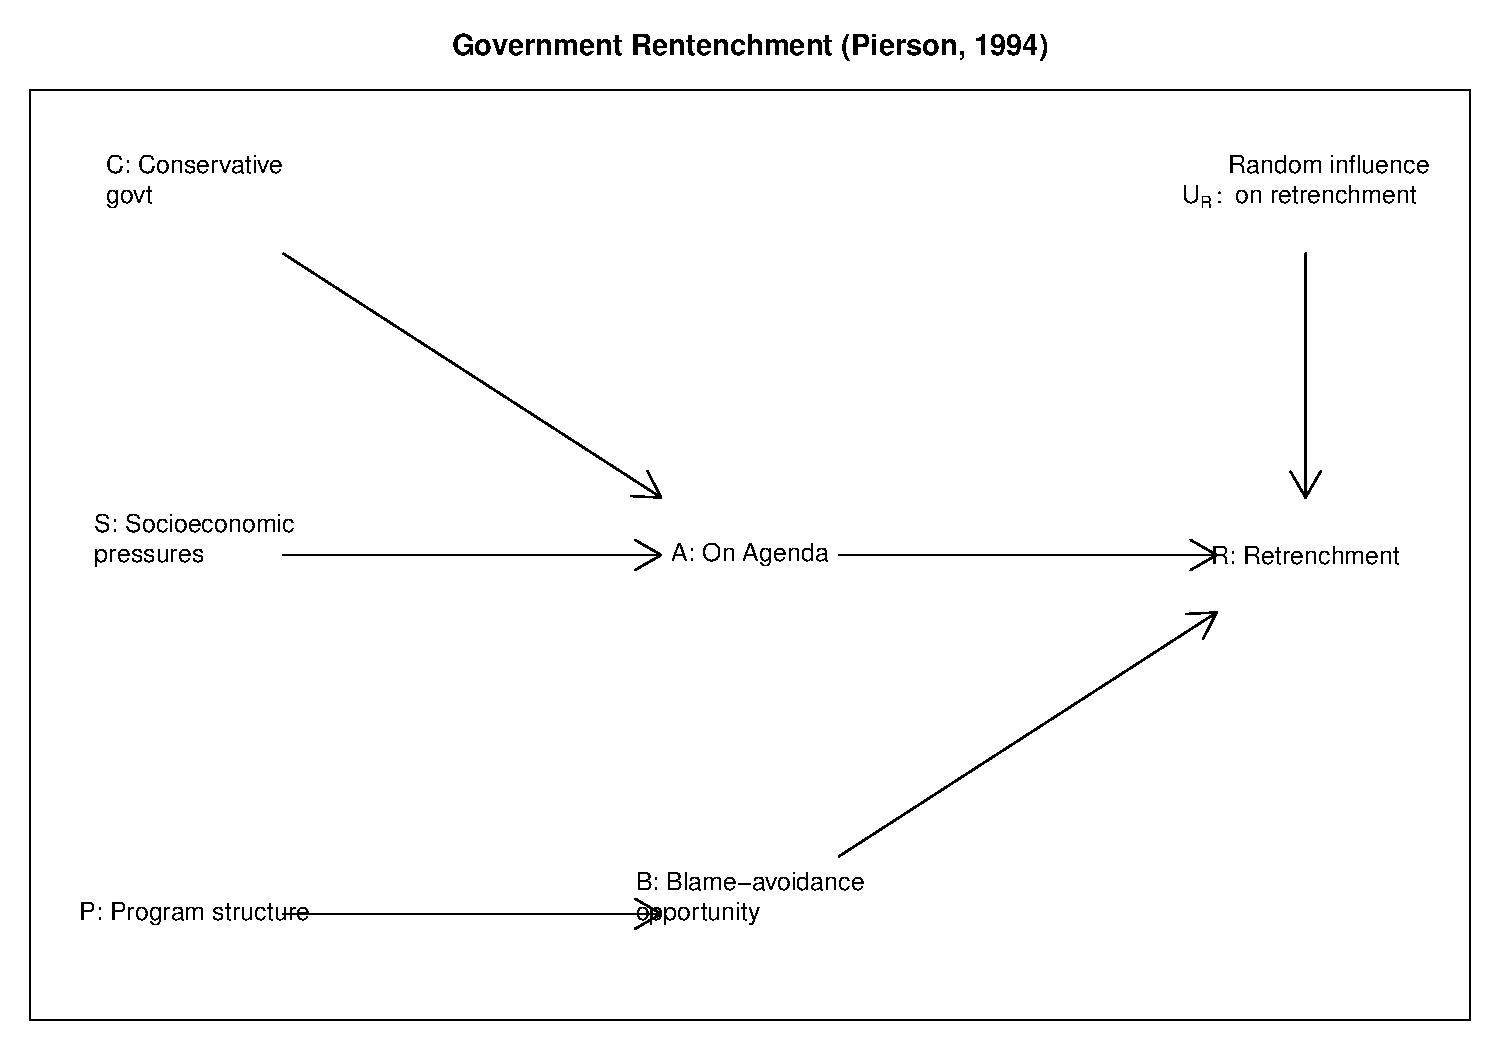
\includegraphics[width=.7\textwidth]{ii_files/figure-latex/unnamed-chunk-8-1} 

}

\caption{\label{fig:DAGPierson} A graphical representation of Pierson (1994).}\label{fig:unnamed-chunk-8}
\end{figure}

While the argument has many more specific features (e.g., different program-structural factors that matter, various potential strategies of blame-avoidance), its essential components can be captured with a relatively simple causal model. We propose such a model in graphical form in Figure \ref{DAGPierson}. Here, the outcome of retrenchment (\(R\)) hinges on whether retrenhcment makes it onto the agenda (\(A\)) and on whether blame-avoidance strategies are available to governments (\(B\)), and on some unspecified random input (\(U_R\)). Retrenchment emerges on the policy agenda as a consequence of both socioeconomic developments (\(S\)) and the ascendance of ideologically conservative political actors (\(C\)). Inherited program structures (\(P\)), meanwhile, determine the availability of blame-avoidance strategies.

A few features of this graph warrant attention. As we have discussed, it is the omitted arrows in any causal graph that imply the strongest statements. The graph in Panel (a) implies that \(C\), \(S\), \(P\), and \(U_R\)---which are neither connected along a directed path nor downstream from a common cause---are independent of one another. This implies, for instance, that whether conservatives govern is independent of whether program structures will allow for blame-free retrenchment. Thus, as Pierson argues, a Reagan or Thatcher can come to power but nonetheless run up against an opportunity structure that would makes retrenchment politically perilous. Further, in this graph any effect of program structures on retrenchment \emph{must} run through their effects on blame-avoidance opportunities. One could imagine relaxing this restriction by, for instance, drawing an arrow from \(P\) to \(A\): program structures might additionally affect retrenchment by conditioning the fiscal costliness of the welfare state, thus helping to determine whether reform makes it onto the agenda.

Where two variables \emph{are} connected by an arrow, moreover, this does not imply that a causal effect will always operate. Consider, for instance, the arrow pointing from \(A\) to \(R\). The fact that \(A\) sometimes affects \(R\) and sometimes does not is, in fact, central to Pierson's argument: conservatives and socioeconomic pressures forcing retrenchment on the agenda will \emph{not} generate retrenchment if blame-avoidance opportunities are absent.

The graph also reflects a choice about where to begin. We could, of course, construct a causal account of how conservatives come to power, how socioeconomic pressures arose, or why programs were originally designed as they were. Yet it is perfectly permissible for us to bracket these antecedents and start the model with \(C\), \(S\), and \(P\), as long as we do not believe that these variables have any antecedents in common. If they do have common causes, then this correlation should be captured in the DAG.\footnote{In DAG syntax, this correlation can be captured by placing the common cause(s) explicitly on the graph or by drawing a dashed line between the correlated nodes, leaving the source of the correlation unspecified.}

The DAG itself tells us about the possible direct causal dependencies but is silent on the ranges of and functional relations among the variables. How might we express these? With three endogenous variables, we need three functions indicating how their values are determined. Moreover, every variable pointing directly into another variable must be part of that second variable's function. Let us assume all variables are binary, with each condition either absent or present. We can capture quite a lot of Pierson's theoretical logic with the following quite simple functional equations:

\begin{itemize}
\tightlist
\item
  \(A=CS\), implying that retrenchment makes it on the agenda if and only if both conservatives are in power and socioeconomic pressures are high.
\item
  \(B=P\), implying that blame-avoidance opporunities arise when and only when program structures take a particular form
\item
  \(R=ABU_R\).
\end{itemize}

This last functional equation requires a little bit of explanation. Here we are saying that retrenchment will only occur if retrenchment is on the agenda and blame-avoidance opportunities are present (as the expression zeroes out if either of these are 0). Yet even if both are present, the effect on retrenchment also hinges on the value of \(U_R\). \(U_R\) thus behaves as a causal-type variable with respect to the effect of an \(AB\) combination on \(R\) and allows for two possible types. When \(U_R=1\), the \(AB\) combination has a positive causal effect on retrenchment. When \(U_R=0\), \(AB\) has no causal effect: retrenchment will not occur regardless of the presence of \(AB\). A helpful way to conceptualize what \(U_R\) is doing is that is capturing a collection of features of a case's context that might render the case susceptible or not susceptible to an \(AB\) causal effect. For instance, Pierson's analysis suggests that a polity's institutional structure might widely diffuse veto power such that stakeholders can block reform even when retrenchment is on the agenda and could be pursued without electoral losses. We could think of such a case as having a \(U_R\) value of 0, implying that \(AB\) has no causal effect. A \(U_R=1\) case, with a positive effect, would be one in which the government has the institutional capacity to enact reforms that it has the political will to pursue.

\hypertarget{saunders-2011}{%
\subsection{Saunders (2011)}\label{saunders-2011}}

\citet{saunders2011leaders} asks why, when intervening militarily abroad, do leaders sometimes seek to transform the \emph{domestic} political institutions of the states they target but sometimes seek only to shape the states' external behaviors. Saunders' central explanatory variable is the nature of leaders' causal beliefs about security threats. When leaders are ``internally focused,'' they believe that threats in the international arena derive from the internal characteristics of other states. Leaders who are ``externally focused,'' by contrast, understand threats as emerging strictly from other states' foreign and security policies. These basic worldviews, in turn, affect the cost-benefit calculations they make about intervention strategies, via two mechanisms. Most simply, these beliefs affect perceptions of the likely security gains from a transformative intervention strategy. In addition, these beliefs affect the kinds of strategic capabilities in which leaders invest, which in turn effects the costliness and likelihood of success of alternative intervention strategies. Calculations about the relative costs and benefits of different strategies then shape the choice between a transformative and non-transformative approach to intervention. Yet leaders can, of course, only choose one of these options if they decide to intervene at all. The decision about whether to intervene depends, in turn, on at least two kinds of considerations. A leader is more likely to intervene against a given target when the nature of the dispute makes the leader's preferred strategy---given their causal beliefs---appear feasible in this situation; yet leaders may also be pushed to intervene by international or domestic audiences.

Figure \ref{fig:DAGSaunders} depicts the causal dependencies in Saunders' argument in DAG form. Working from left to right, we see that causal beliefs (\(C\)) affect the expected net relative benefits of the two strategies (\(B\)) both via a direct pathway and via an indirect pathway running through preparedness investments (\(P\)). Characteristics of a given target state or dispute (\(T\)) likewise influence \(B\). The decision about whether to intervene (\(I\)) is then a function of three factors: causal beliefs (\(C\)), the expected relative net benefits of the strategies (\(B\)), and audience pressures (\(A\)). Finally, the choice of strategy (\(S\)) is a function of whether or not intervention occurs at all (\(I\)), cost-benefit comparisons between the two strategies (\(B\)), and other, idiosyncratic factors that may operate in various cases (\(U_S\)).

\begin{figure}

{\centering 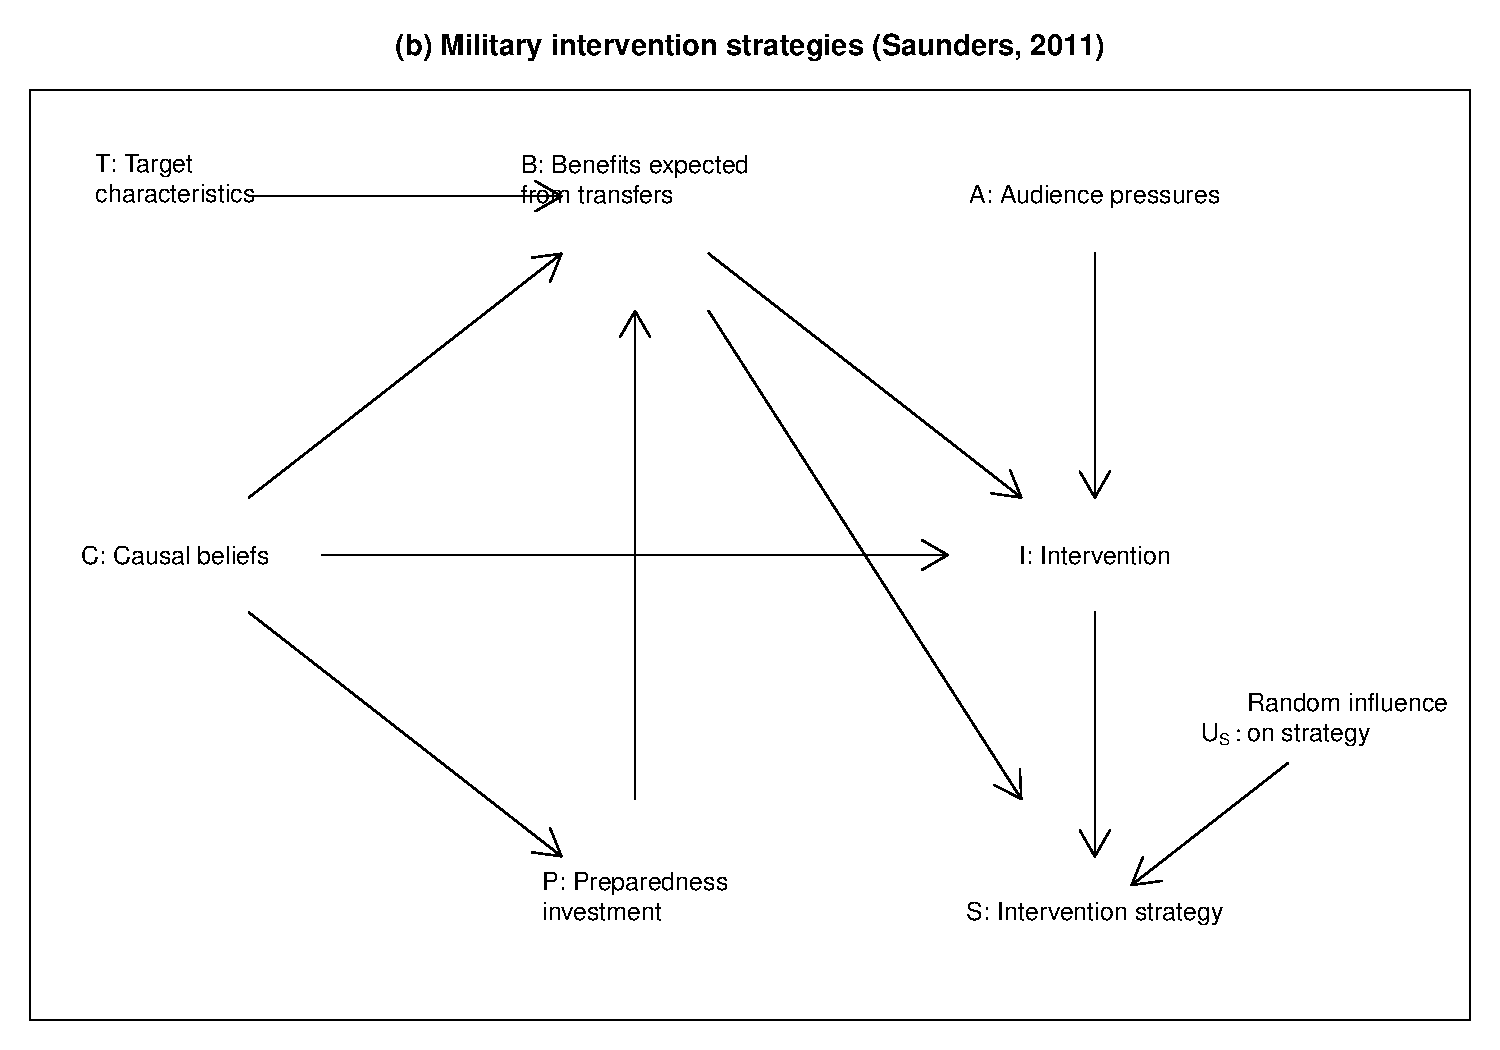
\includegraphics[width=.7\textwidth]{ii_files/figure-latex/unnamed-chunk-9-1} 

}

\caption{\label{fig:DAGSaunders} A graphical representation of Saunders' (2011) argument.}\label{fig:unnamed-chunk-9}
\end{figure}

This relatively complex DAG illustrates how readily DAGs can depict the multiple pathways through which a given variable might affect another variable, as with the multiple pathways linking \(C\) to \(I\) and \(B\) (and, thus, all of its causes) to \(S\). In fact, this graphical representation of the dependencies in some ways throws the multiplicity of pathways into even sharper relief than does a narrative exposition of the argument. For instance, Saunders draws explicit attention to how causal beliefs operate on expected net benefits via both a direct and indirect pathway, both of which are parts of an indirect pathway from \(C\) to the outcomes of interest, \(I\) and \(S\). What is a bit easier to miss without formalization is that \(C\) also acts \emph{directly} on the choice to intervene as part of the feasibility logic: when leaders assess whether their generally preferred strategy would be feasible if deployed against a particular target, the generally preferred strategy is itself a product of their causal beliefs. The DAG also makes helpfully explicit that the two main outcomes of interest---the choice about whether to intervene and the choice about how---are not just shaped by some of the same causes but are themselves causally linked, with the latter depending on the former.

Omitted links are also notable. For instance, the lack of an arrow between \(T\) and \(A\) suggests that features of the target that affect feasibility have no effect on audience pressures. If instead we believed, for instance, that audiences take feasibility into account in demanding intervention, we would want to include a \(T \rightarrow A\) arrow.

Turning to variable ranges and functional equations, it is not hard to see how one might readily capture Saunders' logic in a fairly straightforward set-theoretic manner. All variables except \(S\) could be treated as binary with, for instance, \(C=1\) representing internally focused causal beliefs, \(P=1\) representing preparedness investments in transformation, \(B=1\) representing expectations that transformation will be more net beneficial than non-transformation, \(T=1\) meaning that a target has characteristics that make transformation a feasible strategy, and so on. Although there are two strategies, we in fact need three values for \(S\) because it must be defined for all values of the other variables---i.e., it must take on a distinct categorical value if there is no intervention at all. We could then define functions, such as:

\begin{itemize}
\tightlist
\item
  \(B=CPT\), implying that transformation will only be perceived to be net beneficial in a case if and only if the leader has internally focused causal beliefs, the government is prepared for a transformative strategy, and the target has characteristics that make transformation feasible
\item
  \(I=(1-|B-C|)+(1-(1-|B-C|))A\), implying that intervention can occur under (and only under) either of two alternative sets of conditions: if the generally preferred strategy and the more net-beneficial strategy in a given case are the same (i.e., such that \(B-C=0\)) or, when this alignment is absent (i.e., such that \(|B-C|=0\)), where audiences pressure a leader to intervene.
\end{itemize}

\hypertarget{przeworski-and-limongi-1997}{%
\subsection{Przeworski and Limongi (1997)}\label{przeworski-and-limongi-1997}}

Przeworski and Limongi (\citet{przeworski1997modernization}) argue that democratization occurs for reasons that are, with respect to socioeconomic or macro-structural conditions, largely idiosyncratic; but once a country has democratized, a higher level of economic development makes democracy more likely to survive. Economic development thus affects whether or not a country is a democracy, but only after a democratic transition has occurred, not before. Thus, unlike in \citet{boix2003democracy}, democratization in Przeworski and Limongi's argument is exogenous, rather than being determined by other variables in the model. Moreover, the dynamic component of Przeworski and Limongi's argument---the fact that both the presence of democracy and the causal effect of development on democracy depend on whether a democratic transition occurred at a previous point in time---forces us to think about how to capture over-time processes in a causal model.

We represent Przeworski and Limongi's argument in the DAG in Figure \ref{fig:DAGPL}. The first thing to note is that we can capture dynamics by considering democracy at different points in time as separate nodes. According to the graph, whether a country is a democracy in a given period (\(D_t\)) is a function, jointly, of whether it was a democracy in the previous period (\(D_{t-1}\)) and of the level of per capita GDP in the current period, as well as of other unspecified forces (\(U_{D_t}\)) that lie outside the model.

\begin{figure}

{\centering 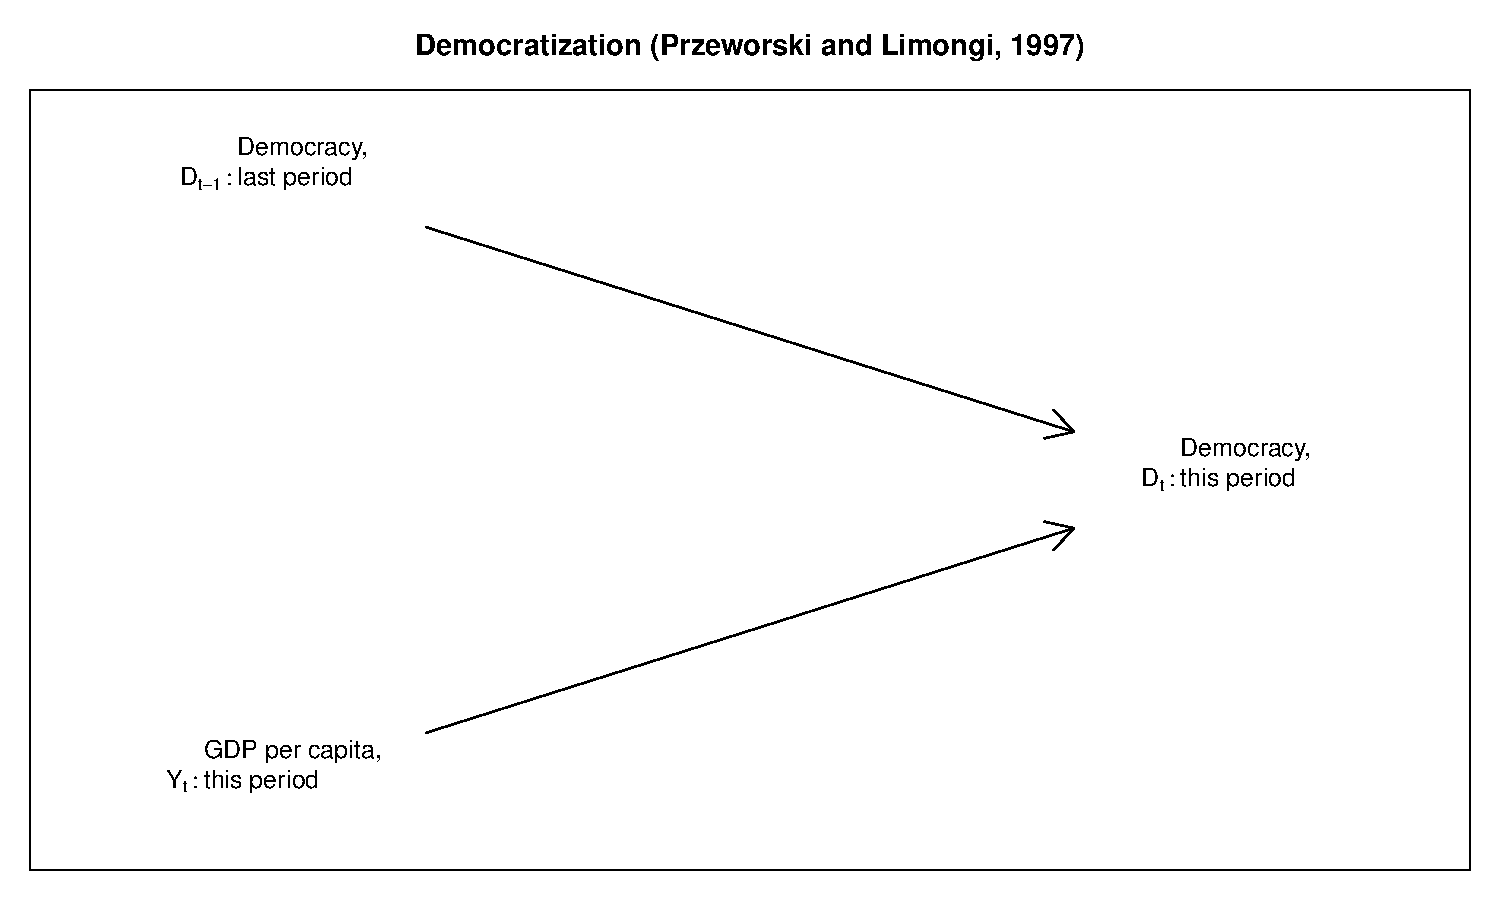
\includegraphics[width=.7\textwidth]{ii_files/figure-latex/DAGPL-1} 

}

\caption{A graphical representation of Przeworski and Limongi's argument, where $D_{t-1}$=democracy in the previous period; $GDP_t$=per capita GDP in the current period; $D_t$=democracy in the current period.}\label{fig:DAGPL}
\end{figure}

Second, the arrow running from \(GDP_{t-1}\) to \(D_t\) means that \(GDP\) \emph{may} affect democracy, not that it always does. Indeed, Przeworski and Limongi's argument is that development's effect depends on a regime's prior state: GDP matters for whether democracies continue to be democracies, but not for whether autocracies go on to become democracies. The \emph{lack} of an arrow between \(D_{t-1}\) and \(GDP_{t-1}\), however, implies a (possibly incorrect) belief that democracy and \(GDP\) in the last period are independent of one another.

Finally, we might consider the kind of causal function that could capture Przeworski and Limongi's causal logic. In this function, \(GDP\) should reduce the likelihood of a transition \emph{away} from democracy but not affect the probability of a transition \emph{to} democracy, which should be exogenously determnined. One possible translation of the argument into functional terms is:

\[d_t = 1 (p(1-d_{t-1}) + d_{t-1}(1-q(1-gdp)) > u_{D_t})\]

where

\begin{itemize}
\tightlist
\item
  \(d_t\) and \(d_{t-1}\) are binary, representing current and last-period democracy, respectively
\item
  \(p\) is a parameter, varying from 0 to 1, representing the probability that an autocracy democratizes
\item
  \(q\) is a parameter, varying from 0 to 1, representing the probability that a democracy with a GDP of 0 reverts to autocracy
\item
  \(gdp\) represents national per capita GDP, normalized on a 0 to 1 scale for the population of interest.
\item
  \(u_{D_t}\) represents a random, additional input into democracy with a uniform distribution on the 0 to 1 scale
\item
  the indicator function, \({1}\), evaluates the inequality and generates a value of \(1\) if and only if it is true
\end{itemize}

Unpacking the equation, the likelihood that a country is a democracy in a given period rises and falls with the expression to the left of the \(>\)-operator. This expression itself has two parts, reflecting the difference between the determinants of \emph{transitions to} democracy (captured by the first part) and the determinants of democratic \emph{survival} (captured by the second). The first part comes into play---i.e., is non-zero---only for non-democracies. For non-democracies, the expression evaluates simply to \(p\), the exogenous probability of democratization. The second part is non-zero only for democracies, where it evaluates to \(1-q\)---the inverse of the reversion parameter---times \(1-gdp\): thus, the reversion probability falls as national income rises. The inequality is then evaluated by ``asking'' whether the expression on the left (either \(p\) or \((1-q)gdp\)) is greater than a number (\(u_{D_t}\)) randomly drawn from a uniform distribution between 0 and 1. Thus, higher values for the expression increase the likelihood of democracy while the randomness of the \(u_{D_t}\) threshold captures the role of other, idiosyncratic inputs.

Note how, while the functional equation nails down certain features of the process, it leaves others up for grabs. In particular, the parameters \(p\) and \(q\) are assumed to be constant for all autocracies and for all democracies, respectively, but their values are left unspecified. And one could readily write down a function that left even more openness---by, for instance, including an unknown parameter that translates \(GDP\) into a change in the probability of reversion or allowing for non-linearities, with unknown parameters, in this effect.

\hypertarget{steps-for-constructing-causal-models}{%
\section{Steps for constructing causal models}\label{steps-for-constructing-causal-models}}

We close with two summaries for how you construct a causal model. First, in Box REF, we summarize the general steps. Second, in Box REF we describe how you can do this in code to produce an object that you can later use for analysis.

\hypertarget{abstract-procedure}{%
\subsection{Abstract procedure}\label{abstract-procedure}}

\begin{center}\rule{0.5\linewidth}{\linethickness}\end{center}

Box: \textbf{Steps for constructing causal models}

\begin{enumerate}
\def\labelenumi{\arabic{enumi}.}
\tightlist
\item
  Identify a set of variables in a domain of interest
\end{enumerate}

\begin{itemize}
\tightlist
\item
  You should specify the range of each variable: is it continuous or discrete?
\item
  May include \(U\) terms representing unspecified, random influences
\end{itemize}

\begin{enumerate}
\def\labelenumi{\arabic{enumi}.}
\setcounter{enumi}{1}
\tightlist
\item
  Draw a causal graph (DAG) representing beliefs about causal dependencies among these variables
\end{enumerate}

\begin{itemize}
\tightlist
\item
  Capture direct effects only
\item
  Arrows indicate \emph{possible}, not constant or certain, causal effects
\item
  The absence of an arrow between two variables indicates a belief of \emph{no} direct causal relationship between them
\item
  Ensure that the graph captures all correlations among variables. This means that either (a) any common cause of two or more variables is included on the graph (with implications for Step 1) or (b) correlated variables are connected with a dashed, undirected edge.
\end{itemize}

\begin{enumerate}
\def\labelenumi{\arabic{enumi}.}
\setcounter{enumi}{2}
\tightlist
\item
  Write down one causal function for each endogenous variable
\end{enumerate}

\begin{itemize}
\tightlist
\item
  Each variable's function must include all variables directly pointing into it on the graph
\item
  Functions may take any form, as long as each set of possible causal values maps onto a single outcome value
\item
  Functions may express arbitrary amounts of uncertainty about causal relations
\end{itemize}

\begin{enumerate}
\def\labelenumi{\arabic{enumi}.}
\setcounter{enumi}{3}
\tightlist
\item
  State probabilistic beliefs about the distributions of the exogenous variables
\end{enumerate}

\begin{itemize}
\tightlist
\item
  How common or likely to do we think different values of the exogenous variables are?
\item
  Are they independently distributed? If in step 2 you drew an undirected edge between nodes then you believe that the connected variables are not independently distributed.
\end{itemize}

\begin{center}\rule{0.5\linewidth}{\linethickness}\end{center}

\hypertarget{model-construction-in-code}{%
\subsection{Model construction in code}\label{model-construction-in-code}}

Our \texttt{gbiqq} package provides a set of functions to implement all of these steps concisely for \emph{binary} models -- models in which all variables are dichotomous.

\begin{Shaded}
\begin{Highlighting}[]
\CommentTok{# Steps 1 and 2 }
\CommentTok{# We define a model with three binary variables and specified edges between them:}
\NormalTok{model <-}\StringTok{ }\KeywordTok{make_model}\NormalTok{(}\StringTok{"X -> M -> Y"}\NormalTok{)}

\CommentTok{# Step 3}
\CommentTok{# Unrestricted functional forms are allowed by default, though these can }
\CommentTok{# also be reduced. Here we impost monotonicity be removing one type for }
\CommentTok{# M and one for Y}
\NormalTok{model <-}\StringTok{ }\KeywordTok{set_restrictions}\NormalTok{(model, }
                          \DataTypeTok{node_restrict =} \KeywordTok{list}\NormalTok{(}\DataTypeTok{M =} \StringTok{"10"}\NormalTok{, }\DataTypeTok{Y=}\StringTok{"10"}\NormalTok{))}

\CommentTok{# Step 4}
\CommentTok{# We set priors over the distribution of (remaining) causal types.}
\CommentTok{# Here we set "jeffreys priors"}
\NormalTok{model <-}\StringTok{ }\KeywordTok{set_priors}\NormalTok{(model, }\DataTypeTok{prior_distribution =} \StringTok{"jeffreys"}\NormalTok{)}

\CommentTok{# We now have a model defined as an R object. }
\CommentTok{# Later we will ask questions of this model and update it using data.}
\end{Highlighting}
\end{Shaded}

These steps are enough to fully describe a binary causal model. Later in this book we will see how we can ask questions of a model like this but also how to use data to train it.

\hypertarget{theory}{%
\chapter{Theories as causal models}\label{theory}}

\begin{center}\rule{0.5\linewidth}{\linethickness}\end{center}

We introduce the idea of thinking of (applied) theoretical claims as claims within hieracrchies of causal models. Lower level models serve as a theory for a higher level model if the higher level model can be deduced from the lower level model. The empirical content of a lower level model is the possible reduction in variance of the higher level model that it can provide.

\begin{center}\rule{0.5\linewidth}{\linethickness}\end{center}

Theory plays an important role in this book's use of causal models for causal inference. Yet the term ``theory'' in the empirical social sciences means very different things in different contexts. In this book, we will refer to a theory is an \emph{explanation} of a phenomeon: a theory provides an account of how or under what conditions a set of causal relationships operate. Moreover, we can express both a theory and the claims being theorized as causal models. A theory, then, is a model that explains and implies another model---possibly with the help of some data.

We discuss toward the end of the chapter how this definition of theory relates to common understandings of theory in the social sciences. First, however, we focus on unpacking our working definition. In embedding theorization within the world of causal models, we ultimately have an empirical objective in mind. Theorizing a causal relationship of interest, in our framework, means elaborating our causal beliefs about the world in greater detail. As we show in later chapters, theorizing in the form of a causal model allows us to generate research designs: to identify sources of inferential leverage and to explicitly and systematically link observations of components of a causal system to the causal questions we seek to answer.

\hypertarget{inequalitytheory}{%
\section{Two theories of inequality's effects on democratization}\label{inequalitytheory}}

To see how this works, let us return to our democratization example and consider first the very basic claim that inequality can have an affect on democratization. We represent this simple claim in Figure \ref{fig:demtheory5}, Panel (a). In this simple model, \(I\) may sometimes have an effect of \(D\), and sometimes not; and that effect may be positive or negative. All of this will depend on the case's causal type. In Chapter \ref{models}, we considered the idea that causal type may be conceptualized as a random disturbance, a \(U\) term, that can take on different type values (e.g., \(a, b, c, d\)) and that points into an outcome variable. To fix this idea going forward, we make a shift in notation and use \(\theta\) to indicate that a node is a receptacle for causal types. Thus, \(\theta_D\) here captures the case's causal type, or \(I\)'s causal effect on \(D\) for a given case.

\begin{figure}

{\centering 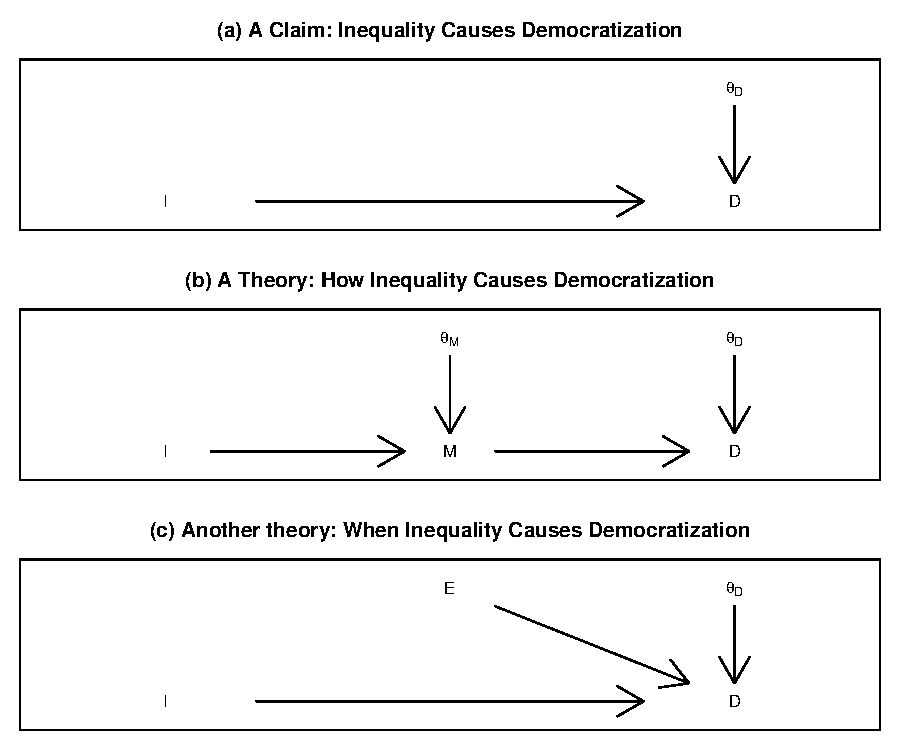
\includegraphics[width=.5\textwidth]{ii_files/figure-latex/demtheory5-1} 

}

\caption{DAG representations of three theories. DAGs only capture claims that one variable causes another, conditional on other variables. Theories (b) and (c) each imply theory (a).}\label{fig:demtheory5}
\end{figure}

We might then wonder \emph{how} inequality might exert its effect on democratization. One possible answer, drawing on our model in Chapter @ref\{models\} is that inequality can affect mass-mobilization, which in turn can affect democratization. This explanatory claim is visually represented in Panel (b) of the figure. Here, we can see that any effect of \(I\) on \(D\) runs through \(M\). There are details of this graph that we will delve into later. But for now, it is sufficient to see that we have partly explained variation left unexplained by model (a). Model (b) allows us to say, for instance, that whether inequality has an effect on democratization has to depend on whether inequality has an effect on mobilization. Model (b) thus theorizes, in one important sense, a part of inequality's effect that is left untheorized in model (a).

Alternatively, we might wonder \emph{when} inequality causes democratization. Our simple claim, in panel (a), allows that \(I\) \emph{can} cause \(D\), but provides no information about the conditions under which it does so. Those conditions are implicitly embedded within \(\theta^D\), where they are left unspecified. We could, however, theorize some of what is left unsaid in in panel (a). We do this in panel (c), where we posit ethnic homogeneity (\(E\)) as a moderator of the inequality's effect on democratization. Panel (c) represents a theory of panel (a) in that it can help account for variation in causal effects that is unaccounted for by the model in (a).

\hypertarget{theory-as-causal-functions}{%
\subsection{Theory as causal functions}\label{theory-as-causal-functions}}

Let's delve a bit deeper into how this works. Thinking through causal functions can help. Consider first a function that might correspond to panel (a). If \(\theta^D\) serves as a simple receptacle for our four basic causal types, then we can deploy our four-causal-type function, familiar from Chapter @ref\{models\}:

\begin{itemize}
\tightlist
\item
  if \(\theta^D=a\), then \(D=1-I\) (\(I\) has a negative causal effect on \(D\))
\item
  if \(\theta^D=b\), then \(D=I\) (\(I\) has a positive causal effect on \(D\))
\item
  if \(\theta^D=c\), then \(D=0\) (\(I\) has no causal effect)
\item
  if \(\theta^D=d\), then \(D=1\) (\(I\) has no causal effect)
\end{itemize}

This model thus allows for \(I\)'s causal effect to vary in ways that are left entirely unaccounted for.

For the moderation model, in panel (c), consider a logic whereby ethnic homogeneity eases mobilization and thus democratization. Drawing on \citet{boix2003democracy}, we theorize that inequality can have a negative effect on democratization by giving the elite more to lose from majority rule, making autocrats less willing to hand over power. Inequality's positive effect, we might further posit, derives from the fact that it gives the poor more to gain from the redistribution that democratization would enable (\citet{acemoglu2005economic}). However, this positive effect can only unfold to the extent that the masses are able to mobilize, and the capacity to mobilize will hinge on ethnic homogeneity. Ethnic homogeneity thus defines the causal possibilities in regard to \(I\)'s effect on \(D\). First, homogeneity is necessary for a positive effect of inequality. Second, by enabling mobilization around distributional demands, ethnic homogeneity rules out a net negative effect of inequality (as inequality's mobilizing effects will balance out elite fears of expropriation). Third, by making mass mobilization easier in general, ethnic homogeneity makes possible mobilization and democratization \emph{without} inequality. Under ethnic heterogeneity, on the other hand, inequality can have a negative effect, or it can no effect at all with autocracy entrenched.

Put differently, under ethnic homogeneity, inequality's effect can only correspond to a \(b\) type or a \(d\) type, while under heterogeneity the effect can only be of type \(a\) or type \(c\). \(E\) thus allows us to partition the range of causal possibilities that model (a) had lumped together under \(\theta^D\). Now we can capture this logic with a functional equation in which \(\theta^D\) now takes on just two possible values (0 or 1), rather than four:

\begin{equation}
D=IE(1-\theta^D)+\theta^DE+(1-E)(1-I)\theta^D
\end{equation}

We can work through the arithmetic to observe \(E\)'s causal-partitioning effect. Whether \(E\) is 0 or 1 determines whether we are in a world of posiitve effects (\(b\) types) and democratization regardless (\(d\) types), or a world of negative effects (\(a\) types) and autocracy regardless (\(c\) types). Note that the righthand side is a sum of three expressions. We can think of \(E\) as a ``switch'' that turns these expressions ``on'' or ``off.'' When \(E=1\), the third expression goes to 0, leaving only the first two in play ``on.'' Now, \(\theta^D\) determines whether \(I\) has a positive effect (when \(\theta^D=0\)) or no effect with \(D\) fixed at \(1\) (when \(\theta^D=1\)). Conversely, when \(E=0\), the first two expressions both go to \(0\), and \(\theta^D\) determines whether \(I\) will have a negative effect (when \(\theta^D=1\)) or no effect with \(D\) stuck at 0 (when \(\theta^D=0\)).

Model (c) has thus given substantive meaning to an aspect of the phenomenon that was merely residual variation in Model (a). Model (a) provides no account of why inequality has the effects it does, relying fully on \(\theta^D\) as a placeholder for this uncertainty. In Model (c), \(\theta^D\) plays a more modest role, with ethnic homogeneity doing a good deal of the work of determining inequality's possible effects.

In sum, Model (b) and Model (c) each \emph{explain} Model (a), if in slightly different ways. Model (b) answers the explanatory question, ``\emph{How} does inequality affect democratization when it does?'' Model (c) answers the explanatory question, ``\emph{Why} does inequality's effect on democratization vary?'' Both theories provide richer, more interpretable accounts of the phenomenon of interest than the simpler model that they are theorizing.

We note one final possibility. Imagine that we started with the quite \emph{specific} claim that inequality sometimes has a positive effect on democratization and sometimes has no effect (with democratization happening for other reasons). Suppose we believed this claim to be true for some, possibly not well defined, domain of cases.\footnote{This claim could be graphically represented by panel (a), but would involve a more restricted range for \(\theta^D\) and simpler functional equation, involving only two types.} Model (c) could serve as a theory of this more specific claim in that Model (c), paired with some data, could explain the claim. In particular, Model (c) paired with the data \(E=1\)---we are in an ethnically homogeneous context---produces the more specific claim. Here, it is the theory \emph{plus an observation} of context that accounts for the specific claim.

\hypertarget{theory-as-a-lower-level-model}{%
\section{Theory as a ``lower-level'' model}\label{theory-as-a-lower-level-model}}

We can, likewise, think of theories as implying the models they are theorizing. If you believe Model (b) in Figure \ref{fig:Demtheory}, then you also must believe Model (a): if inequality can affect mobilization, which can affect democratization, then inequality can affect democratization. Similarly, if you believe Model (c), then you must also believe Model (a): if it is true that inequality can have positive, negative, and null effects on democratization that depend on ethnic homogeneity, then it is also true, more simply, that inequality can have positive, negative, and null effects on democratization.

More formally, let us say that a causal model, \(M^\prime\), is a \emph{theory} of \(M\) if \(M\) is implied by \(M^\prime\). Theory is, thus, all relative. \(M^\prime\) might itself sit atop a theory, \(M^{\prime\prime}\), that implies \(M^\prime\). To help fix the idea of theory as ``supporting'' or ``underlying'' the model(s) it theorizes, we refer to the theory, \(M^\prime\), as a \emph{lower}-level model relative to \(M\) and refer to \(M\) as a \emph{higher}-level model relative to its theorization, \(M^\prime\).\footnote{We note that our definition of theory differs somewhat from that given in \citet{pearl2009causality} (p207): there a theory is a (functional) causal model and a restriction over \(\times_j \mathcal{R}(U_j)\), that is, over the collection of contexts envisionable. Our definition also considers probabilistic models as theories, allowing statements such as `'the average effect of \(X\) on \(Y\) is 0.5.''}

Building on our discussion in Section \ref{inequalitytheory}, we can distill two ways in which lower-level models can relate to, or support, higher-level models:

\hypertarget{disggregating-nodes}{%
\subsection{Disggregating nodes}\label{disggregating-nodes}}

A lower-level model, \(M^\prime\), can be a representation of \(M\) in which a node in \(M\) has been disaggregated into multiple nodes.

\begin{figure}

{\centering 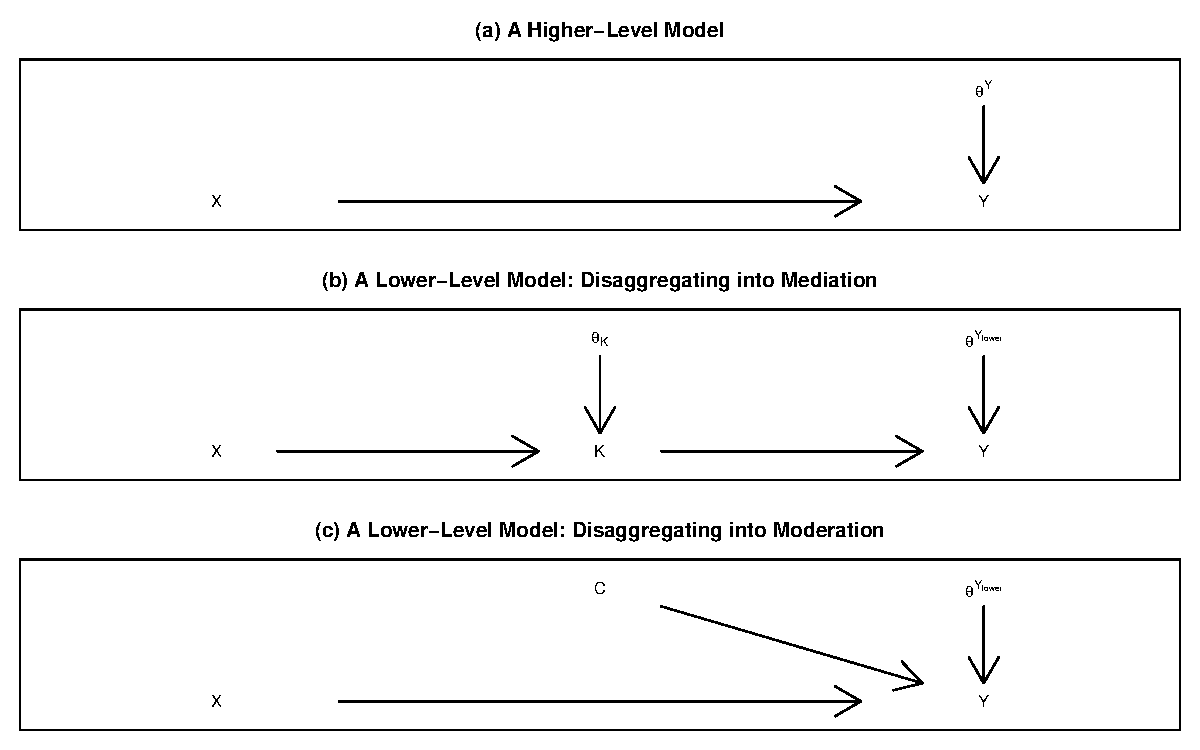
\includegraphics[width=.5\textwidth]{ii_files/figure-latex/unnamed-chunk-12-1} 

}

\caption{\label{fig:Highlow} Here we represent the simple claim that one variable causes another, and two theories --- lower-level models --- that could explain this claim. Both model (b) and model (c) involve theorization via disaggregation of nodes.}\label{fig:unnamed-chunk-12}
\end{figure}

For instance, suppose we start with the higher-level model represented in Figure \ref{fig:Highlow}(a). We can then offer the graph in panel (b) as a \emph{theory}, a lower-level model, of (a). Informally, we have added a step, \(K\), in the causal chain between \(X\) and \(Y\), a familiar mode of theorization, exactly parallel to our model of mediation by mobilization just above. More formally, however, we have in fact \emph{split} one node in (a) into two nodes.

In the higher-level model, (a), \(Y\) is a function of \(X\) and a disturbance \(\theta^Y\), the latter representing all things other than \(X\) than can affect \(Y\). In our four-type setup, \(\theta^Y\) represents all of the (unspecified) sources of variation in \(X\)'s effect on \(Y\). When we add \(K\), \(X\) now does not directly affect \(Y\) but only does so via \(K\). Further, we model \(X\) as acting on \(K\) ``with error,'' with \(\theta^K\) representing all of the (unspecified) factors determining \(X\)'s effect on \(K\). The key thing to notice here is that \(\theta^K\) now represents \emph{a portion of the variance that \(\theta^Y\) represented in the higher-level graph}: some of the variation in \(X\)'s effect on \(Y\) now arises from \(X\)'s effect on \(K\), which is captured by \(\theta^K\). So, for instance, \(X\) might have no effect on \(Y\) because \(\theta^K\) takes on a value such that \(X\) has no effect on \(K\). Likewise, any effect of \(X\) on \(Y\) must arise from an effect of \(X\) on \(K\), captured in \(\theta^K\)'s value. \footnote{As we emphasize further below, it is in fact only this ``error'' in the \(X\rightarrow K\) link that makes the addition of \(K\) potentially informative as a matter of research design: if \(K\) were a deterministic function of \(X\) only, then knowledge of \(X\) would provide full knowledge of \(K\), and nothing could be learned from observing \(K\).} What \(\theta^K\) represents, then, is that part of the original \(\theta^Y\) that arose from some force other than \(X\) operating at the \emph{first} step of the causal chain from \(X\) to \(Y\).

So now, \(\theta^Y\) is not quite the same entity in the lower-level graph that it was in the higher-level graph. In the original graph, \(\theta^Y\) represented \emph{all} sources of variation in \(X\)'s effect on \(Y\). In the lower-level model, with \(K\) as mediator, \(\theta^Y\) represents only random variation in \(K\)'s effect on \(Y\). \(\theta^Y\) has been expunged of any factors shaping the first stage of the causal process, which now reside in \(\theta^K\). Reflecting a convention that we use throughout the book, we highlight this change in \(\theta^Y\)'s meaning by referring in the second model to \(\theta^{Y_\text{lower}}\).

Theorization here thus starts with the proliferation of substantive variables---adding beliefs about intervening steps in a causal process. But, critically, it also involves an accompanying disaggregation of unexplained variation. Addition and splitting thus go hand-in-hand: the \emph{insertion} of a mediator between \(X\) and \(Y\) also involves the \emph{splitting} of \(Y\)'s unspecified parent (\(\theta_Y\)).

Consider next panel (c) in Figure \ref{fig:Highlow}, which also supports (implies) the higher-level theory in panel \((a)\). The logical relationship between models \((a)\) and \((c)\), however, is somewhat different. Here the lower-level model \emph{specifies} one of the conditions that comprised \(\theta^Y\) in the higher-level model. In specifying a moderator, \(C\), we have extracted \(C\) from \(\theta^Y\), leaving \(\theta^{Y_\text{lower}}\) to represent all factors \emph{other than \(C\)} that condition \(X\)'s effect on \(Y\). (Again, the relabeling as \(\theta^{Y_\text{lower}}\) reflects this change in the term's meaning.) While we might add a \(\theta^C\) term pointing into \(C\), this is not necessary. Whereas in Model (b) we have extracted \(\theta^K\) from \(\theta^Y\), in Model (c), it is \(C\) itself that we have extracted from \(\theta^Y\), substantively specifying what had been just a srandom disturbance.

\hypertarget{generalizing-a-model}{%
\subsection{Generalizing a model}\label{generalizing-a-model}}

A lower-level model, \(M^\prime\), can also be a representation of \(M\) in which a node has been introduced that permits variation in a feature of context that is fixed and taken-for-granted in \(M\). Here, \(M^\prime\) theorizes \(M\) in the sense of embedding \(M\) within a \emph{more general} set of beliefs about how the world works. \(M\) then becomes a special case of the theorized relations, one that holds when we condition on some data, specifying some particularity of context.

To illustrate this approach to theorization, consider again graphs (a) and (c) in Figure \ref{fig:Highlow}. We have discussed how the graph in panel (c) can represent a disaggregation of \(\theta^Y\) from panel (a) into \(\theta^{Y_\text{lower}}\) and \(C\). An alternative possibility, however, is to employ a moderation model that represents a more general claim than the higher-level model that it supports. For instance, the graph in panel (a) might represent the causal function \(Y=X+\theta^Y\). In this model, \(X\) always has an effect on \(Y\). The graph in panel (c), in turn, might represent the more general function, \(Y=XC+\theta^Y\) (where \(C\) is binary). Now, whether \(X\) has an effect depends on the value of \(C\). In particular, model (c) combined with the observation \(C=1\) directly implies model (a). Model (a) is a special case of model (c) that holds in and only in the context \(C=1\). In answer to the question, ``Why do you believe model (a)?'' one could respond with model (c) plus the observation \(C=1\).

Note the difference in how theorization has proceeded for the two moderation models (both graphically represented in panel (c)). When we introduce moderation via the disaggregation of nodes, we pull content out of \(\theta^Y\) and specify it substantively. When we generalize, on the other hand, we \emph{add} a node, a source of variation not factored into the original model at all. We can think of that variation as implicitly conditioned-on in the higher-level model.

As a secondary matter, note that the \(\theta\) term pointing into \(Y\) may or may not be altered by the addition. In particular, we will explore later, if \(\theta^Y\) is a vessel for causal types, then the number of possible causal types---and, thus, \(\theta^Y\)'s range---must expand as we add nodes pointing into \(Y\). But in the functions we have used in our illustration, \(\theta^{Y_\text{lower}}\) remains unchanged when we add the \(C\) node. In both the higher- and lower-level models, \(\theta^Y\) represents precisely the same random disturbance.

\hypertarget{moving-between-higher--and-lower-level-models}{%
\section{Moving between higher- and lower-level models}\label{moving-between-higher--and-lower-level-models}}

As we will see, thinking about models as conditionally nested within one another can be empirically useful. It provides a way of generating empirical leverage on a causal question by plumbing more deeply our background knowledge about a domain of interest. When we more fully specify higher-level claims via a more elaborate, lower-level model, we are a making explicit unspecified conditions on which the higher-level relationships depend. In doing this, we are identifying potentially observable nodes that might be informative about our research question.

\hypertarget{mappings-are-not-one-to-one}{%
\subsection{Mappings are not one-to-one}\label{mappings-are-not-one-to-one}}

As we develop lower-level models to support our claims, or determine which claims are supported by our theories, what kinds of moves are we permitted to make? One important thing to note is that the mappings between higher-level claims and theories may not be one-to-one. A single theory can support multiple higher-level theories. Moreover, a single higher-level relation can be supported by multiple, possibly incompatible lower-level theories.

To illustrate, consider two ``lower level'' theories of democratization:

\begin{itemize}
\tightlist
\item
  (\(L_1\)): \(Inequality \rightarrow Democratization \leftarrow Mobilization\)\\
\item
  (\(L_2\)): \(Inequality \rightarrow Mobilization \rightarrow Democratization\)
\end{itemize}

Note how these theories are incompatible with one another. While \(Inequality\) and \(Democratization\) are independent in \(L_1\), they are causally related in \(L_2\). Moreover, in \(L_2\), \(Inequality\) and \(Democratization\) are related only through \(Mobilization\), while in \(L_1\), \(Democratization\) is directly affected by \(Inequality\).\footnote{Put differently, these two theories record different relations of conditional independence: in \(L_1\), \(Inequality\) and \(Mobilization\) are unconditionally independent, but they are not unconditionally independent in \(L_2\). Also, in \(L_2\), \(Inequality\) is independent of \(Democratization\) conditional on \(Mobilization\); but this is not the case in \(L_1\).}

Now, consider the following three higher-level claims:

\begin{itemize}
\tightlist
\item
  (\(H_1\)): \(Inequality \rightarrow Democratization\)
\item
  (\(H_2\)): \(Mobilization \rightarrow Democratization\)
\item
  (\(H_3\)): \(Inequality \rightarrow Mobilization\)
\end{itemize}

\(H_1\) could be derived from (explained by) either theory, \(L_1\) or \(L_2\). Although the two theories are incompatible with one another, in both theories \(Inequality\) affects \(Democratization\). Both theories likewise imply \(H_2\), in which \(Mobilization\) affects \(Democratization\).

\(H_3\), however, can be supported only by one of these theories: only in \(L_1\), and not in \(L_2\), does \(Inequality\) cause \(Mobilization\).\footnote{In addition, the \emph{conditional} higher-level model \(((Inequality \rightarrow Democratization)|Mobilization=1)\) can be supported by model \(L_1\) but not by model \(L_2\), where holding \(Mobilization\) constant would sever the dependence of \(Democratization\) on \(Inequality\).}

Thus multiple (possibly \emph{incompatible}) theories can usually be proposed to explain any given causal effect. When seeking an explanation for, say, \(H_1\), the choice between \(L_1\) and \(L_2\) is not dictated by logic; it must be drawn from a substantive belief about which set of causal dependencies operates in the world. On the other hand, \(L_2\) \emph{is} logically ruled out as an explanation of \(H_3\). Further, any given theory logically implies multiple (necessarily \emph{compatible}) higher-level claims about causal relations.

\hypertarget{permissible-moves-across-levels}{%
\subsection{Permissible moves across levels}\label{permissible-moves-across-levels}}

What, more generally, are the permissible moves across levels?

\hypertarget{moving-down-levels}{%
\subsubsection{Moving down levels}\label{moving-down-levels}}

We have already discussed two possible forms of theorization --- moves down a level: (i) disaggregating existing nodes, introducing beliefs about mediation or moderation, or (ii) adding nodes representing variation in a feature of context that is implicitly held constant in the higher-level model.

There are other possible ways of elaborating a model. For instance, we can add \emph{antecedent conditions}: causes of nodes that were exogenous in the higher-level model. Likewise, we can add \emph{downstream effects}: outcomes of nodes that were terminal in the higher-level model.

\begin{figure}

{\centering 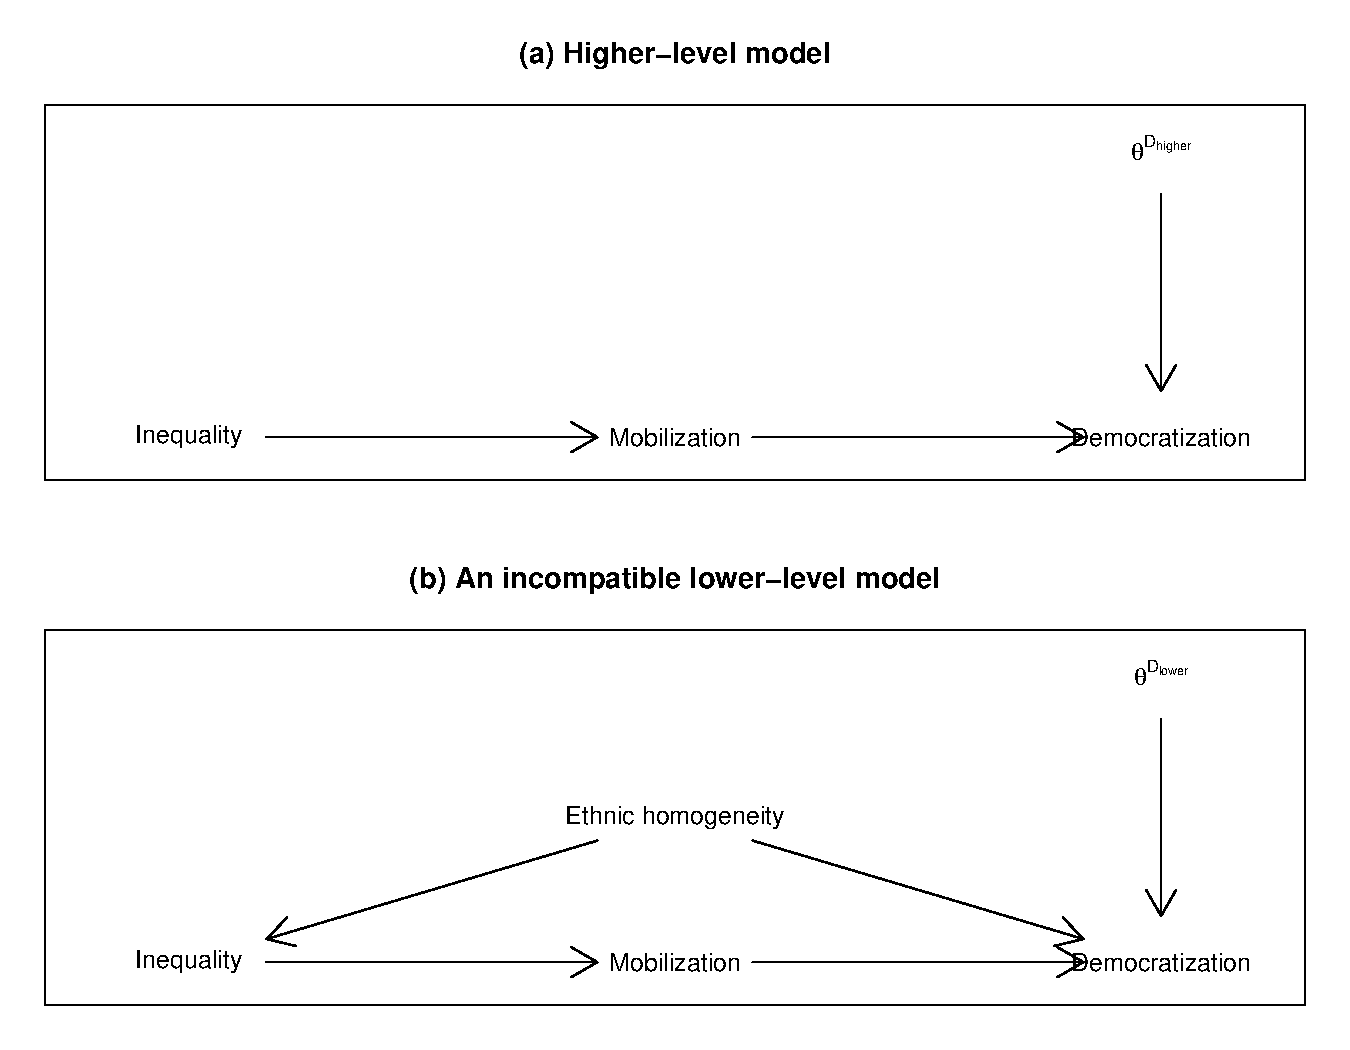
\includegraphics[width=.7\textwidth]{ii_files/figure-latex/incompat-1} 

}

\caption{A higher-level model and a lower-level model that is impermissible.}\label{fig:incompat}
\end{figure}

The central principle governing allowable elaborations is that a lower-level model \emph{must not introduce dependencies between variables that were omitted in the higher-level model.} We provide an example of a violation of this principle in Figure \ref{fig:incompat}.

We start with a higher-level model, in panel (a), in which inequality affects democratization through mobilization. We then elaborate the model in panel (b) by adding ethnic homogeneity as a moderator of mobilization's effect. However, because ethnic homogeneity is also modeled here as affecting inequality, we have now introduced a source of dependence between inequality and democratization that was omitted from the higher-level model. In panel (a), democratization and inequality were dependent only via mobilization; and so they are conditionally independent given mobilization. In panel (b), democratization and mobilization are additionally dependent via their common cause, ethnic homogeneity. By the rules governing causal graphs (see Chapter \ref{models}), the higher-level specifically \emph{prohibited} this second source of dependency---since all dependencies between variables must be represented.
Put differently, if two variables are independent--- or conditionally independent given a third variable---in one model, then this same relation of independence (or conditional independence) must be captured in any theory of that model. A theory can \emph{add} conditional independencies not present in the higher-level model. For instance, a mediation theory, \(X \rightarrow M \rightarrow Y\), implies a conditional independence that is not present in the higher-level model that it supports, \(X \rightarrow Y\): in the lower-level model only, \(X\) is conditionally independent of \(Y\) given \(M\). But we may not theorize away (conditional) independencies insisted on by our higher-level claim.

\hypertarget{moving-up-levels}{%
\subsubsection{Moving up levels}\label{moving-up-levels}}

Moving in the other direction, what, in general, are the permissible \emph{simplifications} of lower-level models? In other words, given a theory, what are the higher-level claims that it can support?

When we move up a level --- i.e., eliminate one or more nodes --- the key rule is that the higher-level graph must take into account:

\begin{enumerate}
\def\labelenumi{(\alph{enumi})}
\tightlist
\item
  all \emph{dependencies} among remaining nodes and
\item
  all \emph{variation} generated by the eliminated node.
\end{enumerate}

We can work out what this means, separately, for eliminating \emph{endogenous} nodes and for eliminating \emph{exogenous} nodes.

\hypertarget{eliminating-endogenous-nodes}{%
\paragraph{Eliminating endogenous nodes}\label{eliminating-endogenous-nodes}}

Eliminating an endogenous nodes means removing a node with parents (direct causes) represented on the graph. If the node also has one or more children, then the node captures a dependency: it links its parents to its children. When we eliminate this node, preserving these dependencies requires that all of the eliminated node's parents adopt---become parents of---all of the eliminated node's children. Thus, for instance in panel (b) of Figure \ref{fig:Highlow}, if we were to eliminate \(M\), \(M\)'s parents (\(X\) and \(\theta^M\)) need to adopt \(M\)'s child, \(Y\). We see in panel (a) of the figure, the higher-level model, that \(X\) is now pointing directly into \(Y\).

As for \(\theta^M\), it too must now point directly into \(Y\)---though we can use a bit of shorthand to make this happen. Recall that \(\theta^M\) represents the part of \(M\) that is randomly determined. Rather than drawing two separate disturbance (\(\theta\)) terms pointing into \(Y\), however, we more simply represent the combined disturbance term as \(\theta^Y_{\text{higher}}\), with the `'higher'' signaling the aggregation of roots. (This is, of course, simply reversing the disaggregation that we undertook earlier to move from the higher- to the lower-level model.)

More intuitively, when we simplify away a mediator, we need to make sure that we preserve the causal relationships being mediated---both those among substantive variables and any random shocks at the mediating causal steps.\footnote{Eliminating endogenous nodes may also operate via ``encapsulated conditional probability distributions'' \citep{koller2009probabilistic} wherein a system of nodes, \(\{Z_i\}\) is represented by a single node, \(Z\), that takes the parents of \(\{Z_i\}\) not in \(\{Z_i\}\) as parents to \(Z\) and issues the children of \((Z_i)\) that are not in \((Z_i)\) as children. However, this is not a fundamental alteration of the graph.}

\hypertarget{eliminating-exogenous-nodes}{%
\paragraph{Eliminating exogenous nodes}\label{eliminating-exogenous-nodes}}

What about eliminating exogenous nodes---nodes with no parents? For the most part, exogenous nodes cannot be eliminated, but must either be replaced by or incorporated into \(U\) (or \(\theta\)) terms. The reason is that we need preserve any dependencies or variation generated by the exogenous node. Figure \ref{fig:elimrules} walks through four different situations in which we might want to simplify away the exogenous node, \(X\). (Here we use the more generic \(U\) notation, though the same principles apply if these are type-receptacles(\(\theta\).)

\begin{figure}

{\centering 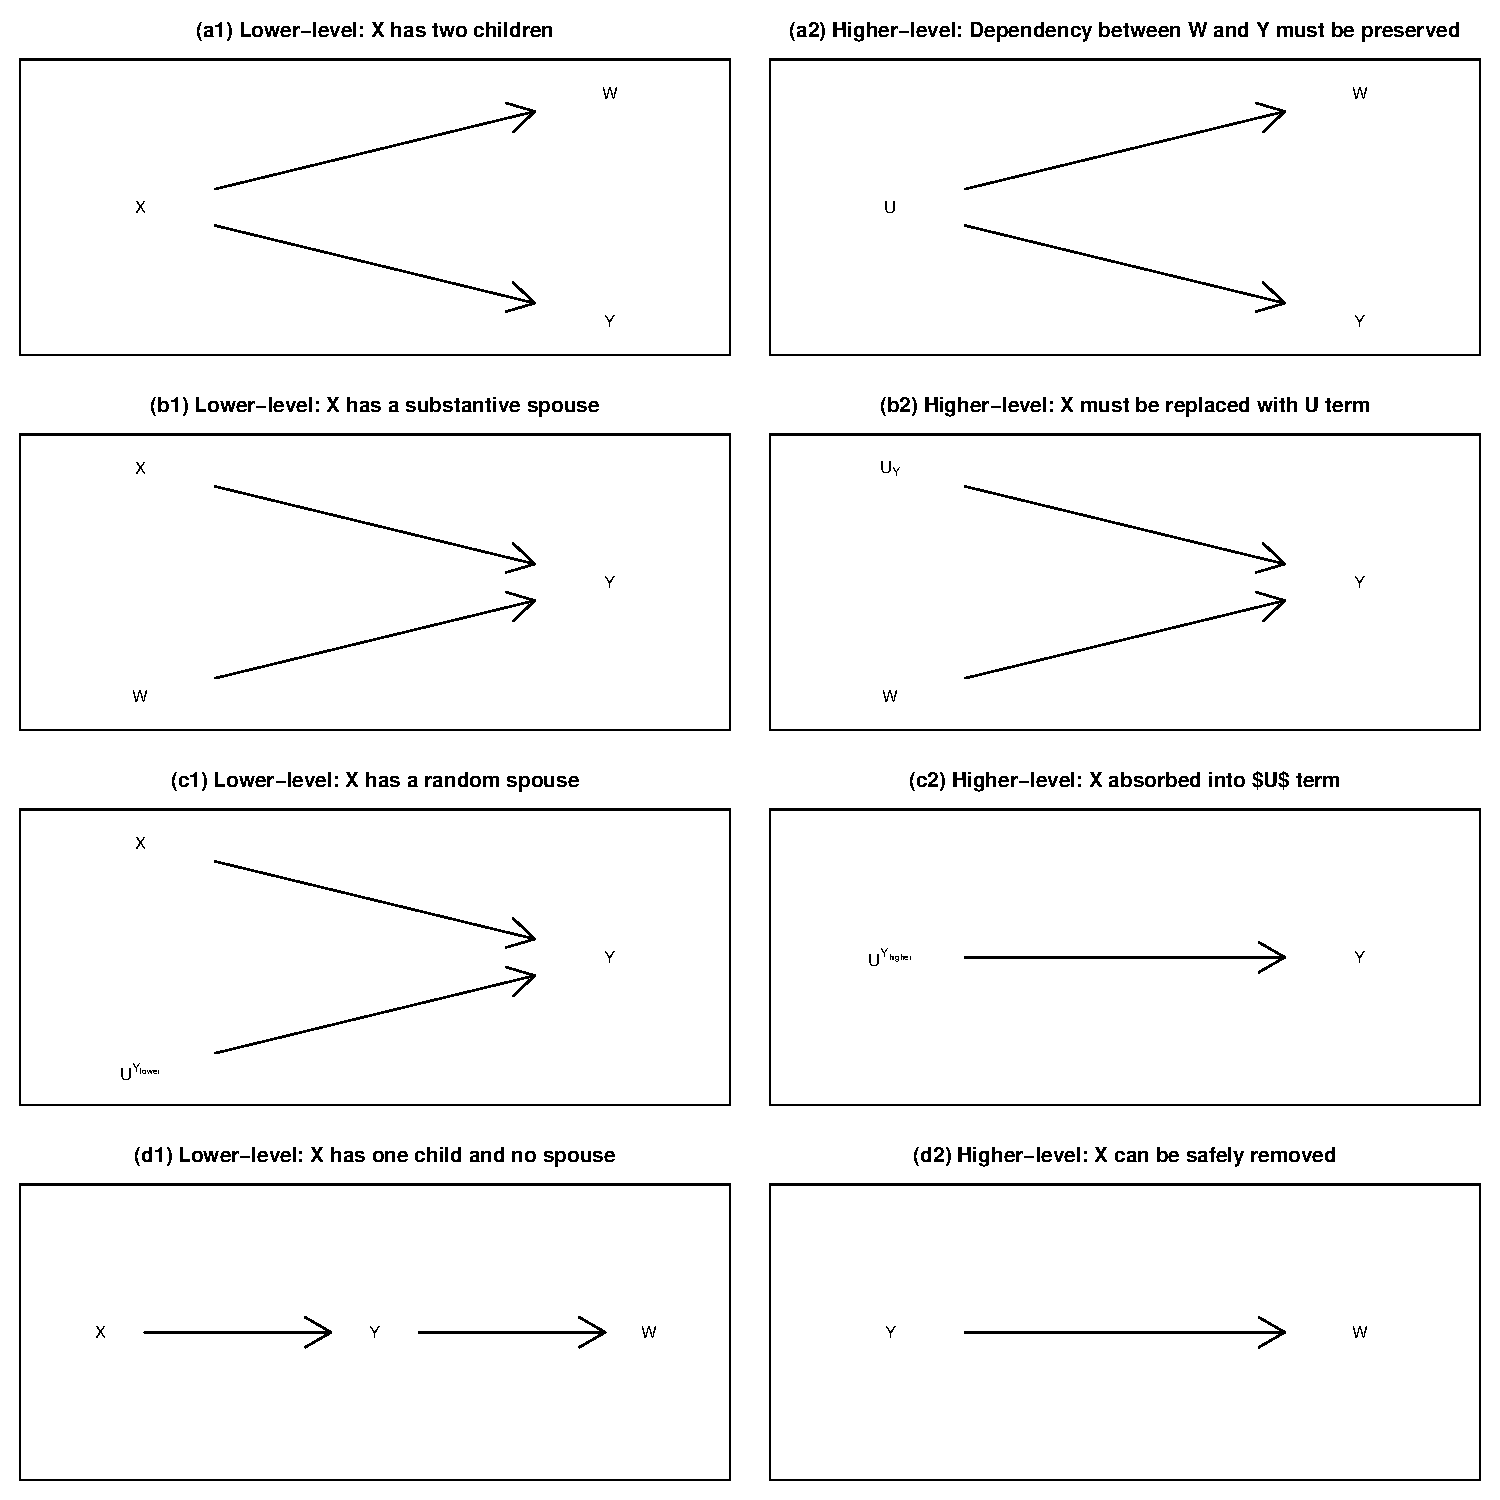
\includegraphics[width=.5\textwidth]{ii_files/figure-latex/elimrules-1} 

}

\caption{Here we represent the basic principles for eliminating exogenous nodes.}\label{fig:elimrules}
\end{figure}

\begin{itemize}
\tightlist
\item
  \emph{Multiple children.} In (a1), we start with a lower-level model in which \(X\) has two children, thus generating a dependency between \(W\) and \(Y\). If we eliminate \(X\), we must preserve this dependency. We can do so, as pictured in (a2), by replacing \(X\) with a \(U\) term that also points into \(W\) and \(Y\).\footnote{By DAG convention, we could, alternatively, convey the same information with a dashed, undirected line between \(W\) and \(Y\).} Though we are no longer specifying what it is that connects \(W\) and \(Y\), the correlation itself is retained.
\item
  \emph{Substantive spouse.} In (b1), \(X\) has a spouse that is substantively specified, \(W\). If we eliminate \(X\), we have to preserve the fact that \(Y\) is not fully determined by \(W\); \emph{something} else also generates variation in \(Y\). We thus need to replace \(X\) with a \(U\) term, \(U_Y\), to capture the variation in \(Y\) that is not accounted for by \(W\).
\item
  \emph{\(U\)-term spouse.} In (c1), \(X\) has a spouse that is \emph{not} substantively specified, \(U^{Y_\text{lower}}\). Eliminating \(X\) requires, again, capturing the variance that it generates as a random input. As we already have a \(U\) term pointing only into \(Y\), we can substitute in \(U^{Y_\text{higher}}\), which represents both \(U^{Y_\text{lower}}\) and the variance generated by \(X\).\emph{IS THIS FOOTNOTE RIGHT?}\footnote{This aggregation cannot occur if \(U^{Y_\text{lower}}\) also has another child, \(W\), that is not a child of \(X\) since then we would be representing \(Y\)'s and \(W\)'s random components as identical, which they are not in the lower-level graph.}
\item
  \emph{One child, no spouse.} In (d1), \(X\) has only one child and no spouse. Here we can safely eliminate \(X\) with no loss of information. It is always understood that every exogenous node has some cause, and there is no loss of information in simply eliminating a node's causes if those causes are exogenous and do not affect other endogenous nodes in the model. In (d2) we are simply not specifying \(Y\)'s cause, but we have not lost any dependencies or sources of variance that had been expressed in (d1).
\end{itemize}

One interesting effect of eliminating a substantive exogenous node can be to render seemingly deterministic relations effectively probabilistic. In moving from (b1) to (b2), we have taken a component of \(Y\) that was determined by \(X\) and converting it into a random disturbance. Just as we can explain a more probabilistic claim with a less probabilistic theory, we can derive higher-level claims with greater probabilism from theories with greater determinism.

\begin{verbatim}
## Warning in text.default(x, y + text_shift, names, cex =
## cex): font metrics unknown for character 0xa

## Warning in text.default(x, y + text_shift, names, cex =
## cex): font metrics unknown for character 0xa

## Warning in text.default(x, y + text_shift, names, cex =
## cex): font metrics unknown for character 0xa

## Warning in text.default(x, y + text_shift, names, cex =
## cex): font metrics unknown for character 0xa
\end{verbatim}

\begin{figure}

{\centering 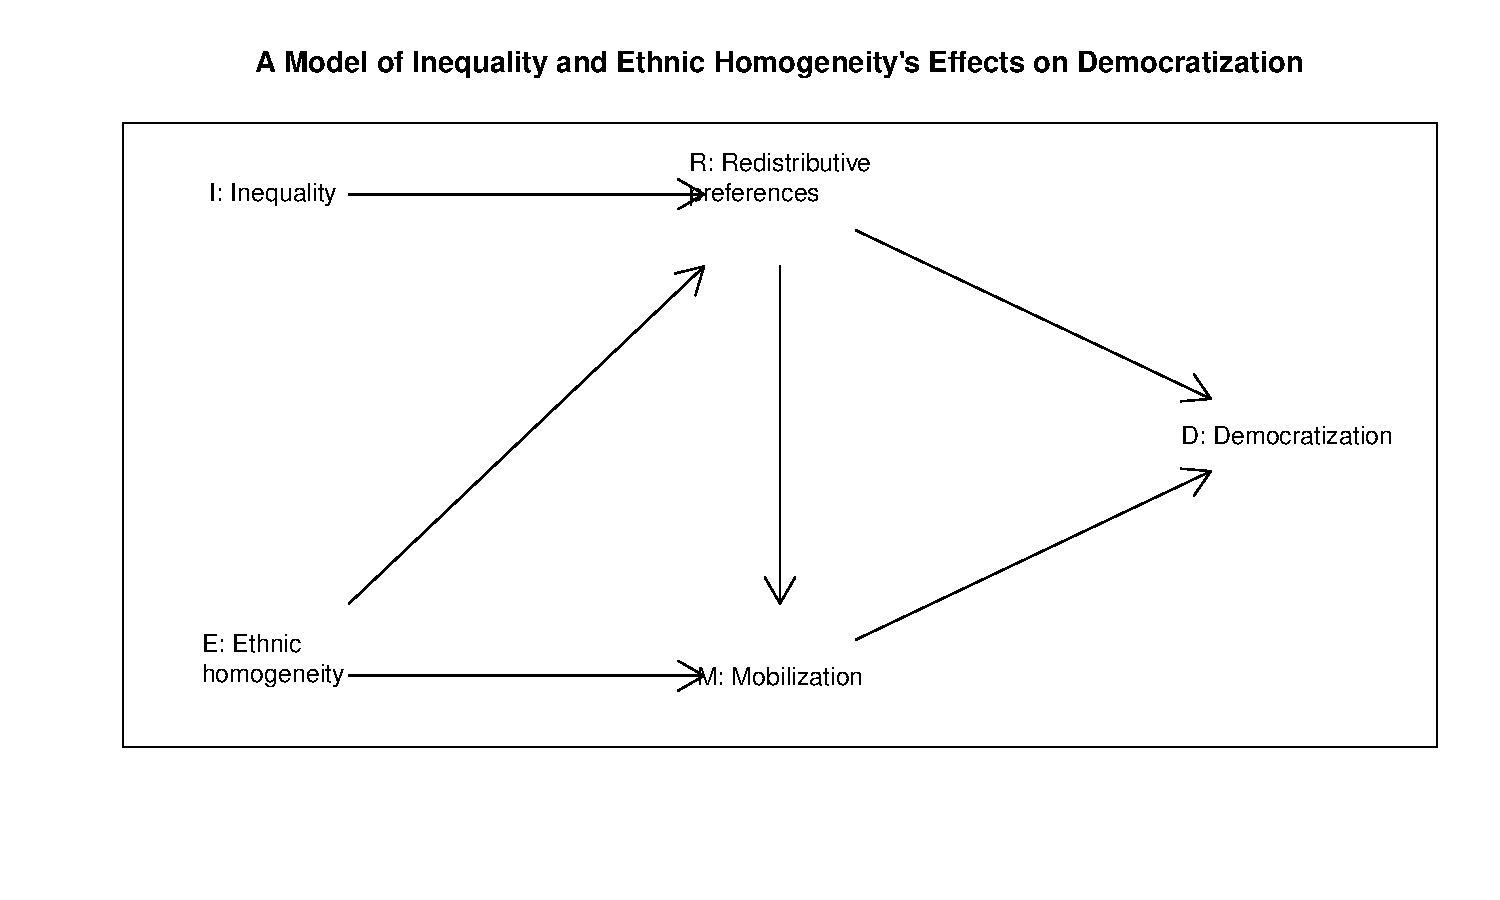
\includegraphics[width=.5\textwidth]{ii_files/figure-latex/lowercomplexdem-1} 

}

\caption{A lower-level model  from which multiple higher level models can be derived.}\label{fig:lowercomplexdem}
\end{figure}

\begin{figure}
\centering
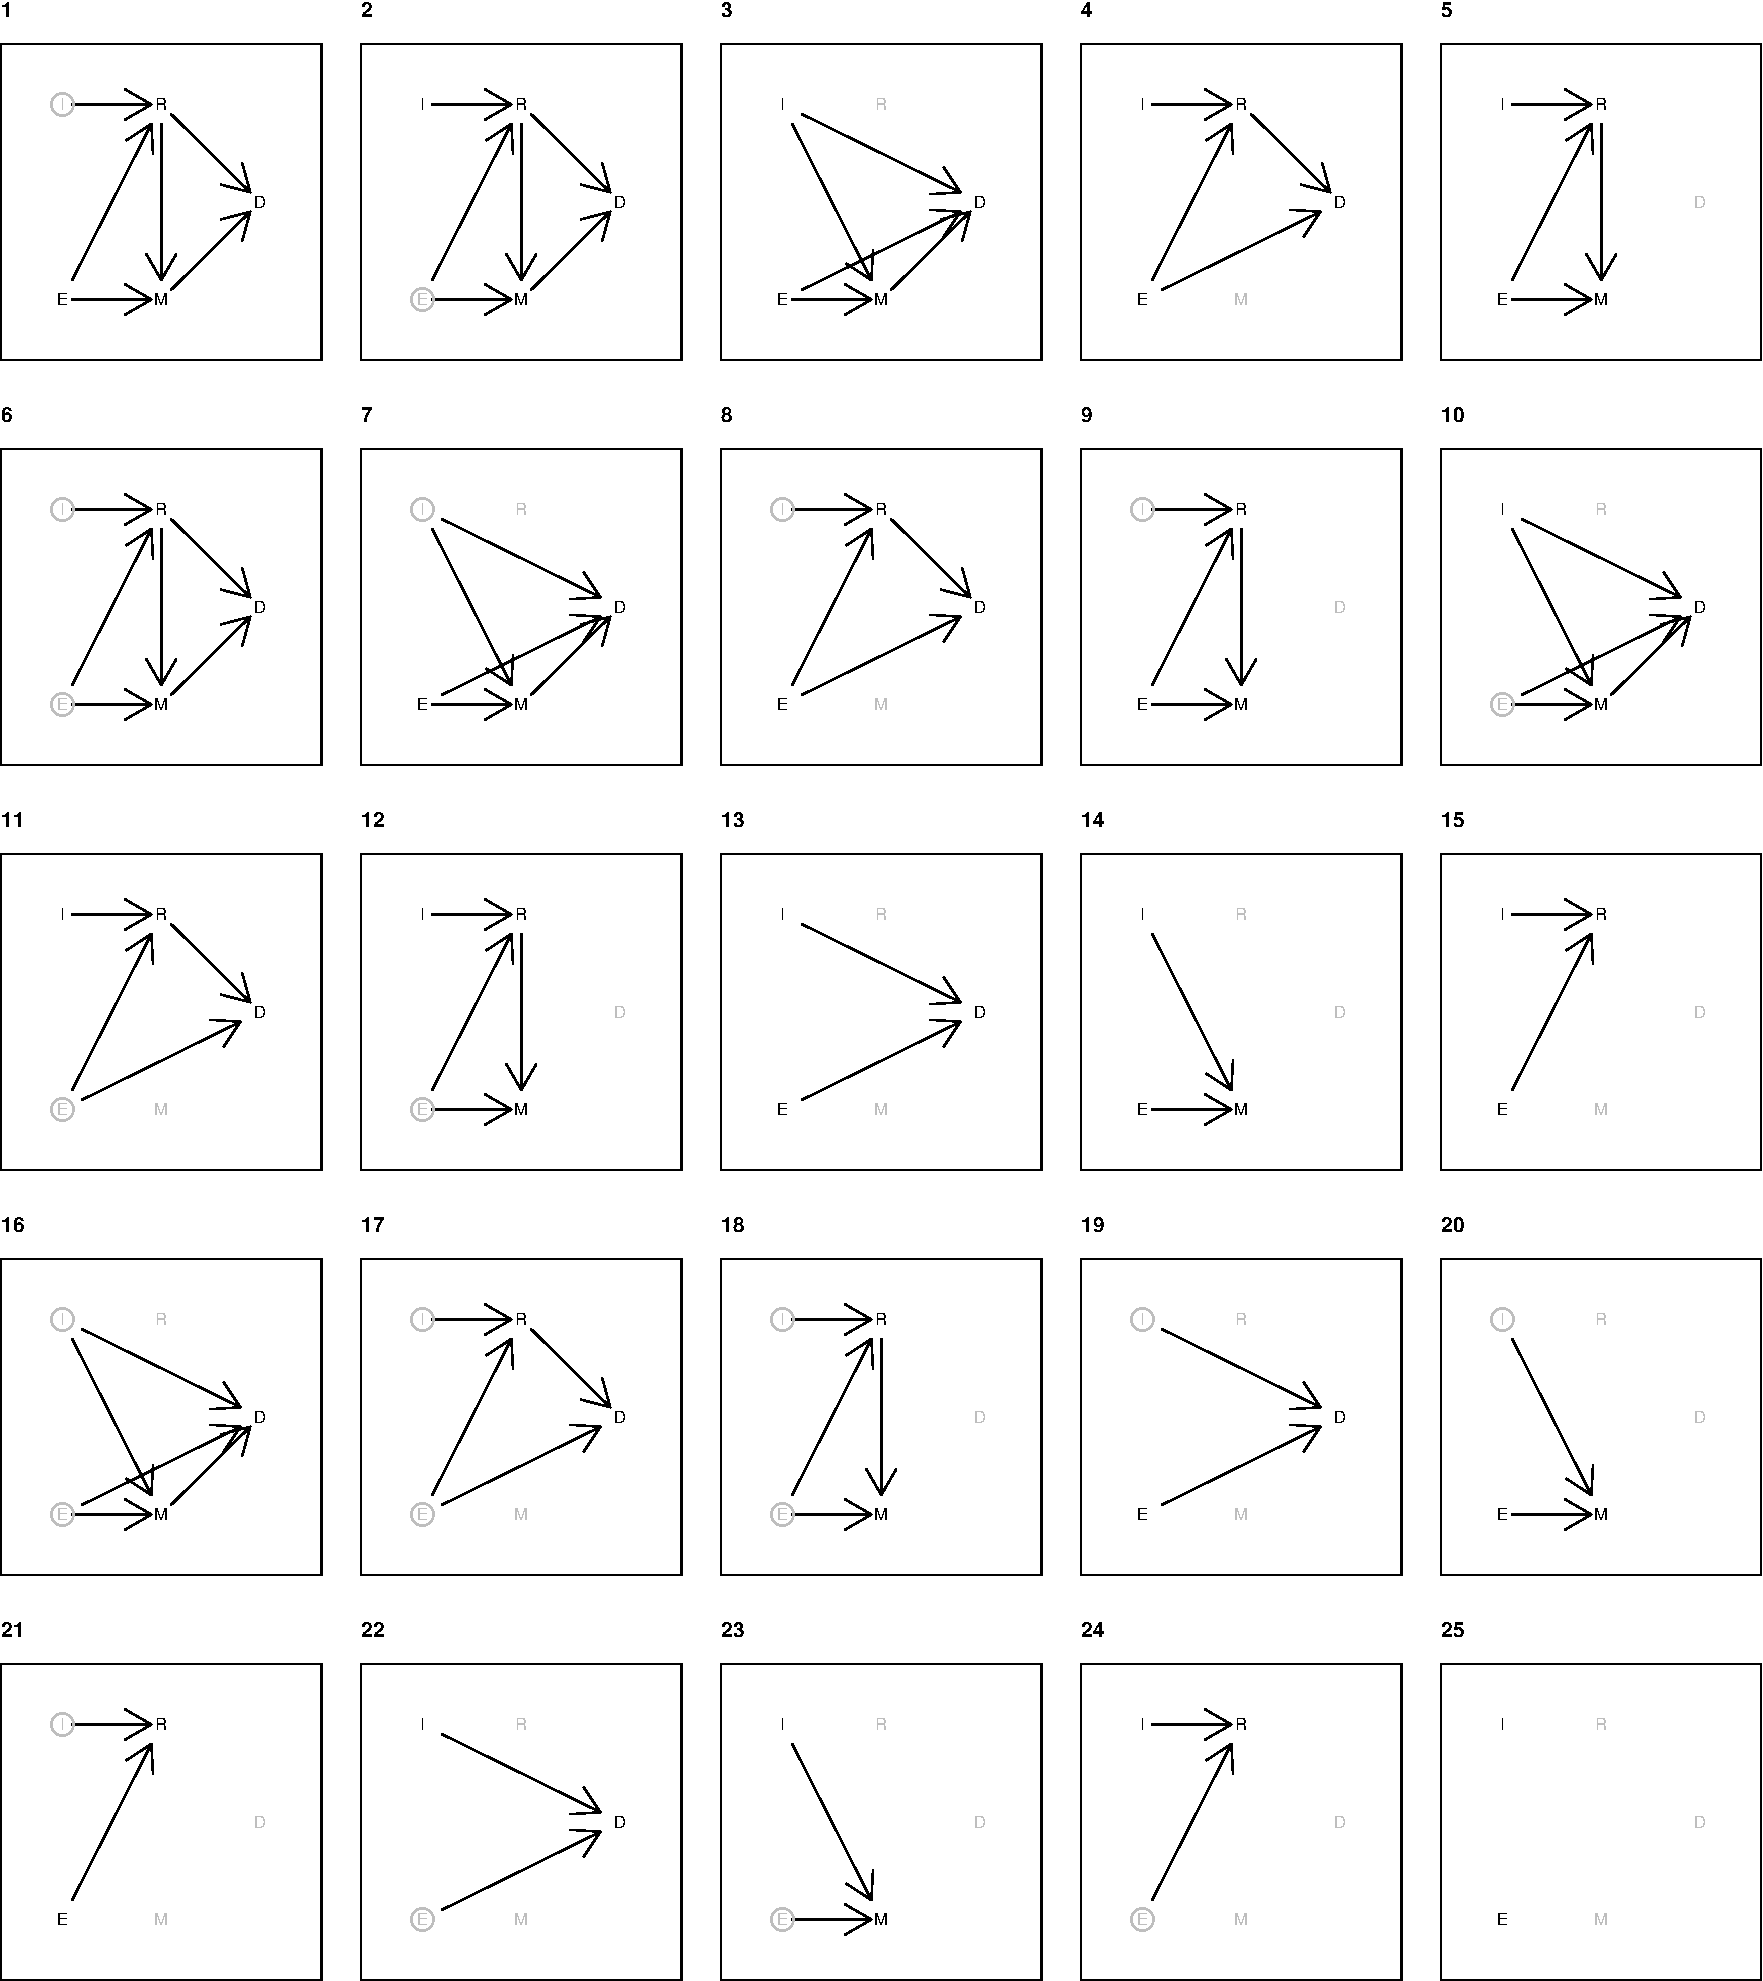
\includegraphics{ii_files/figure-latex/runningsubs-1.pdf}
\caption{\label{fig:runningsubs}Higher level models derived from the lower level model of Figure X. Nodes that are eliminated are marked in grey; circles denote exogenous nodes that are replaced in subgraphs by unidentified variables. (A circled node pointing into two other nodes could equivalently be indicated as an undirected edge connecting the two.) Note that \(M\), \(R\), and \(D\) are deterministic functions of \(I\) and \(E\) in this example, with no random inputs pointing into them.}
\end{figure}

We can apply these principles to a model of any complexity. We illustrate a wider range of simplifications by starting with Figure \ref{fig:lowercomplexdem}, which represents a somewhat amended version of our inequality and democratization model from Chapter \ref{models}, with more complex causal relations. Then, in Figure \ref{fig:runningsubs}, we show all permissible reductions of the more elaborate model. We can think of these reductions as the full set of simpler claims (involving at least two nodes) that can be derived from the lower-level theory. In each subgraph,

\begin{itemize}
\tightlist
\item
  we mark eliminated nodes in grey;
\item
  those nodes that are circled must be replaced with \(U\) terms; and
\item
  arrows represent the causal dependencies that must be preserved.
\end{itemize}

Note, for instance, that neither \(E\) (because it has a spouse) nor \(I\) (because it has multiple children) can be simply eliminated; each must be replaced with a \(U\) term. Also, the higher-level graph with nodes missing can contain arrows that do not appear at all in the lower-level graph: eliminating \(M\), for instance, forces an arrow running from \(X\) to \(R\) and another running from \(X\) to \(Y\), as \(X\) must adopt \(M\)'s children. The simplest elimination is of \(D\) itself since it does not encode any dependencies between other variables.

We can also read Figure \ref{fig:runningsubs} as telling us the set of claims for which the lower-level graph in Figure \ref{fig:running} can serve as a theory. As we can see, the range of claims that a moderately complex model can theorize is vast. For each simpler claim, moreover, there may be other possible lower-level graphs---theories besides ---consistent with it.

\hypertarget{conditioning-on-nodes}{%
\paragraph{Conditioning on nodes}\label{conditioning-on-nodes}}

A further permissible ``upward'' move is conditioning on a node. When we condition on a node, we are restricting the higher-level model in scope to situations in which that node's value is held constant. Doing so allows us to eliminate the node as well as all arrows pointing into it or out of it. Consider three different situations in which we might condition on a node:

\begin{itemize}
\tightlist
\item
  \emph{Exogneous, with multiple children.} In simplifying (a1) in Figure \ref{fig:elimrules}, we need to be sure we retain any dependence that \(X\) generates between \(W\) and \(Y\). However, recalling the rules of conditional independence on a graph (see Chapter \ref{models}), we know that \(W\) and \(Y\) are \emph{independent} conditional on \(X\). Put differently, if we restrict the analysis to contexts in which \(X\) takes on a constant value, the lower-level model implies that \(Y\) and \(W\) will be uncorrelated across cases. As fixing \(X\)'s value breaks the dependence between \(Y\) and \(W\), we can drop \(X\) (and the arrows pointing out of it) without having to represent that dependence.
\item
  \emph{Exogenous, with spouse.} In simplifying (b1) or (c1) Figure \ref{fig:elimrules}, we need to account for the variation generated by \(X\). If we fix \(X\)'s value, however, then we eliminate this variation by assumption and do not need to continue to represent it (or the arrow pointing out of it) on the graph.
\item
  \emph{Endogenous.} When we condition on an endogenous node, we can eliminate the node as well the arrows pointing into and out of it. We, again, leverage relations of conditional independence here. If we start with graph (b) in Figure \ref{fig:Highlow}, and we condition on the mediator, \(M\), we sever the link between \(Y\) on \(X\), rendering them conditionally independent of one another. We can thus remove \(M\), the arrow from \(X\) to \(M\), and the arrow from \(M\) to \(Y\). In the new model, with \(M\) fixed, \(Y\) will be entirely determined by the random disturbance \(\theta^{Y_\text{lower}}\).\footnote{Note that such conditioning does not add any variance to the \(\theta^Y\) term, so we retain the notation \(\theta^{Y_\text{lower}}\).}
\end{itemize}

In sum, we can work with models that are simpler than our causal beliefs: we may believe a complex lower-level model to be true, but we can derive from it a sparer set of claims. There may be intervening causal steps or features of context that we believe matter, but that are not of interest for a particular line of inquiry. While these can be removed, we nonetheless have to make sure that their \emph{implications} for the relations remaining in the model are not lost. Understanding the rules of reduction allow us to undertake an important task: checking which simpler claims are and are not consistent with our full belief set.

\textbf{BOXES}

\begin{center}\rule{0.5\linewidth}{\linethickness}\end{center}

\textbf{BOX 1}

\textbf{Two kinds of theories.}

Theories are ``lower-level'' causal models that explain or provide an account of a ``higher-level'', simpler model. There are two forms of theorization:

\begin{enumerate}
\def\labelenumi{\arabic{enumi}.}
\tightlist
\item
  The disaggregation of nodes. A single node in a higher-level model can be split into multiple nodes. For instance, for a higher-level model in which \(X \rightarrow Y \leftarrow \theta^Y\):
\end{enumerate}

\begin{itemize}
\tightlist
\item
  \emph{Mediation}: A mediator, \(M\), can be introduced between \(X\) and \(Y\), thus splitting \(\theta^Y\) into \(\theta^M\) and \(\theta^{Y_\text{lower}}\). The mediation theory thus explains the \(X \rightarrow Y\) relationship.
\item
  \emph{Moderation}: A component of \(\theta^Y\) can be extracted and specified as a substantive variable. This variable is now a substantively conceptualized moderator of the \(X \rightarrow Y\) relationship. The moderation theory thus provides a fuller explanation of why \(X\) has different effects on \(Y\) in different contexts.
\end{itemize}

\begin{enumerate}
\def\labelenumi{\arabic{enumi}.}
\setcounter{enumi}{1}
\tightlist
\item
  Generalization. A feature of context omitted and implicitly held constant in a higher-level model can be explicitly included in the model. The higher-level model is now explained as a special case of a more general set of causal relations.
\end{enumerate}

\begin{center}\rule{0.5\linewidth}{\linethickness}\end{center}

\begin{center}\rule{0.5\linewidth}{\linethickness}\end{center}

\textbf{BOX 2}

\textbf{Rules for moving between levels}

\emph{Moving down levels}:

All (conditional) independencies represented in a higher-level model must be preserved in the lower-level model.

When we disaggregate or add nodes to a model, new conditional independencies can be generated. But any variables that are independent or conditionally independent (given a third variable) in the higher-level model must also be independent or conditionally independent in the lower-level model.

\emph{Moving up levels}: We can move up levels by eliminating an exogenous node, eliminating an endogenous node, or conditioning on a node. When we eliminate a node from a model, we must preserve any variation and dependencies that it generates:

\begin{enumerate}
\def\labelenumi{\arabic{enumi}.}
\tightlist
\item
  When eliminating an endogenous node, that node's parents adopt (become direct causes of) that node's children.
\item
  When eliminating an exogenous node, we must usually replace it with a \(U\) term. If the node has more than one child, it must be replaced with a \(U\) term pointing into both children (or an undirected edge connecting them) to preserve the dependency between its children. If the node has a spouse, the eliminated node's variation must also be preserved using a \(U\) term. Where the spouse is (already) a \(U\) term with no other children, \(U\) terms can be combined.\\
\item
  Since conditioning on a node ``blocks'' the path through which it connects its children, we can simply eliminate the node and the arrows between it and its children.
\item
  An exogenous node with no spouse and only one child can be simply eliminated.
\end{enumerate}

\begin{center}\rule{0.5\linewidth}{\linethickness}\end{center}

\hypertarget{beneath-the-graph-causal-types-in-lower-level-models}{%
\section{Beneath the Graph: Causal Types in Lower-Level Models}\label{beneath-the-graph-causal-types-in-lower-level-models}}

We have discussed theorization largely from a graphical perspective, showing how features of causal graphs change (nodes get split, combined, added, or removed) as we move down or up levels. But there is more that happens beneath the surface of a graphical structure when we theorize a claim. In this section, we return to our causal-type framework, in which causal types are captured by \(\theta\) terms. While we have already shown how we can introduce causal types into the simplest \(X \rightarrow Y\) model, we work through here how the causal-type space changes as we complicate that model. We show, first, how causal types operate a mediation model, and then how they operate in a model with moderation.

\hypertarget{medtheory}{%
\subsection{Mediation as Theory}\label{medtheory}}

We begin with a simple claim: there are two binary variables, \(X\) and \(Y\), and \(X\) may have an effect on \(Y\). This claim is represented in Figure \ref{fig:Highlow}(a) above. In this graph, \(X\) is independent of \(\theta^Y\), which means that it is as if \(X\) is randomly assigned.

We will let \(\theta^Y\) be a variable that ranges across our four different causal types, conditioning how \(Y\) responds to \(X\). While \(a, b, c\), and \(d\) were heuristically useful as a way of introducing the idea of a causal type, things will soon get more complicated, so it will be useful to have more flexible notation. Going forward, we will usually refer to causal types using \(\theta\) notation, with subscripts and superscripts used to denote potential outcomes and outcome variables. In our binary \(X \rightarrow Y\) setup, we can indicate the causal type governing \(Y\)'s response with notation of the form \(\theta^Y_{ij}\), where \(i\) and \(j\) represent \(Y\)'s potential outcomes. Specifically, \(i\) represents the value \(Y\) takes on when \(X=0\), while \(j\) represents the value \(Y\) takes on when \(X=1\).\footnote{The functional equation for \(Y\) is then given by:
  \[Y(x, \theta_{ij}^{Y_\text{higher}}) = \left\{ \begin{array}{cc}  
  i & \text{ if } x=0 \\ j & \text{ if } x=1 \end{array}  \right.\]} Thus, the translation from \(a, b, c\) and \(d\) notation is:

\begin{itemize}
\tightlist
\item
  \emph{a}: \(\theta_{10}^Y\). A negative effect implies that \(Y\) is \(1\) when \(X=0\) and \(0\) when \(X=1\).
\item
  \emph{b}: \(\theta_{01}^Y\). A positive effect implies that \(Y\) is \(0\) when \(X=0\) and \(1\) when \(X=1\).
\item
  \emph{c}: \(\theta_{00}^Y\). A null ``chronic'' effect implies that \(Y\) is \(0\) regardless of \(X\)'s value.
\item
  \emph{d}: \(\theta_{11}^Y\). A null ``destined'' effect implies that \(Y\) is \(1\) regardless of \(X\)'s value.
\end{itemize}

To be clear, these \(\theta_{ij}^Y\) terms are not random variables; they are the four \emph{values} (types) that the type-variable \(\theta^Y\) can take on.

Now consider a theory that specifies a variable intervening between \(X\) and \(Y\). This theory is depicted in Figure \ref{fig:Highlow}(b) above, where \(M\) mediates the relationship. We see that there are now two \(\theta\) terms, each representing a set of causal types for a different step in the causal chain. While \(\theta^Y\) represented \(Y\)'s response to its parent \(X\), \(\theta^Y_{\text{lower}}\) represents \(Y\)'s response to its ``new'' parent, \(M\). We now also need to conceive of a causal type capturing \(M\)'s response to \(X\), and we let \(\theta^M\) represent this type.\footnote{This graph assumes no confounding in the mediating relationship either as the two \(\theta\) terms and \(X\)'s assignment are all independent of one another.}

We thus allow \(X\) to have a positive, negative, or no effect on \(M\), with \(\theta^M\) taking on four possible values:

\begin{itemize}
\tightlist
\item
  \emph{a}: \(\theta_{10}^M\)
\item
  \emph{b}: \(\theta_{01}^M\)
\item
  \emph{c}: \(\theta_{00}^M\)
\item
  \emph{d}: \(\theta_{11}^M\)
\end{itemize}

And we allow for \(M\) to have a positive, negative, or no effect on \(Y\), with \(\theta^Y_{\text{lower}}\)'s possible values being:

\begin{itemize}
\tightlist
\item
  \emph{a}: \(\theta_{10}^Y\)
\item
  \emph{b}: \(\theta_{01}^Y\)
\item
  \emph{c}: \(\theta_{00}^Y\)
\item
  \emph{d}: \(\theta_{11}^Y\)
\end{itemize}

We can now think about \emph{combinations} of types in the lower-level model as mapping onto types in the higher-level model. We work through these mappings in greater detail later in the book, but consulting table \ref{tab:highlowmapping}, one can readily see how this works.

\begin{longtable}[]{@{}lllll@{}}
\caption{\label{tab:highlowmapping} Mapping from lower level nodal types on \(M\) and \(Y\) to higher level causal types on \(Y\).}\tabularnewline
\toprule
\begin{minipage}[b]{0.13\columnwidth}\raggedright
\strut
\end{minipage} & \begin{minipage}[b]{0.18\columnwidth}\raggedright
\(\theta_{10}^{Y_{lower}}\)\strut
\end{minipage} & \begin{minipage}[b]{0.18\columnwidth}\raggedright
\(\theta_{01}^{Y_{lower}}\)\strut
\end{minipage} & \begin{minipage}[b]{0.18\columnwidth}\raggedright
\(\theta_{00}^{Y_{lower}}\)\strut
\end{minipage} & \begin{minipage}[b]{0.18\columnwidth}\raggedright
\(\theta_{11}^{Y_{lower}}\)\strut
\end{minipage}\tabularnewline
\midrule
\endfirsthead
\toprule
\begin{minipage}[b]{0.13\columnwidth}\raggedright
\strut
\end{minipage} & \begin{minipage}[b]{0.18\columnwidth}\raggedright
\(\theta_{10}^{Y_{lower}}\)\strut
\end{minipage} & \begin{minipage}[b]{0.18\columnwidth}\raggedright
\(\theta_{01}^{Y_{lower}}\)\strut
\end{minipage} & \begin{minipage}[b]{0.18\columnwidth}\raggedright
\(\theta_{00}^{Y_{lower}}\)\strut
\end{minipage} & \begin{minipage}[b]{0.18\columnwidth}\raggedright
\(\theta_{11}^{Y_{lower}}\)\strut
\end{minipage}\tabularnewline
\midrule
\endhead
\begin{minipage}[t]{0.13\columnwidth}\raggedright
\(\theta_{10}^{M}\)\strut
\end{minipage} & \begin{minipage}[t]{0.18\columnwidth}\raggedright
\(\theta_{01}^{Y_{higher}}\)\strut
\end{minipage} & \begin{minipage}[t]{0.18\columnwidth}\raggedright
\(\theta_{10}^{Y_{higher}}\)\strut
\end{minipage} & \begin{minipage}[t]{0.18\columnwidth}\raggedright
\(\theta_{00}^{Y_{higher}}\)\strut
\end{minipage} & \begin{minipage}[t]{0.18\columnwidth}\raggedright
\(\theta_{11}^{Y_{higher}}\)\strut
\end{minipage}\tabularnewline
\begin{minipage}[t]{0.13\columnwidth}\raggedright
\(\theta_{01}^{M}\)\strut
\end{minipage} & \begin{minipage}[t]{0.18\columnwidth}\raggedright
\(\theta_{10}^{Y_{higher}}\)\strut
\end{minipage} & \begin{minipage}[t]{0.18\columnwidth}\raggedright
\(\theta_{01}^{Y_{higher}}\)\strut
\end{minipage} & \begin{minipage}[t]{0.18\columnwidth}\raggedright
\(\theta_{00}^{Y_{higher}}\)\strut
\end{minipage} & \begin{minipage}[t]{0.18\columnwidth}\raggedright
\(\theta_{11}^{Y_{higher}}\)\strut
\end{minipage}\tabularnewline
\begin{minipage}[t]{0.13\columnwidth}\raggedright
\(\theta_{00}^{M}\)\strut
\end{minipage} & \begin{minipage}[t]{0.18\columnwidth}\raggedright
\(\theta_{11}^{Y_{higher}}\)\strut
\end{minipage} & \begin{minipage}[t]{0.18\columnwidth}\raggedright
\(\theta_{00}^{Y_{higher}}\)\strut
\end{minipage} & \begin{minipage}[t]{0.18\columnwidth}\raggedright
\(\theta_{00}^{Y_{higher}}\)\strut
\end{minipage} & \begin{minipage}[t]{0.18\columnwidth}\raggedright
\(\theta_{11}^{Y_{higher}}\)\strut
\end{minipage}\tabularnewline
\begin{minipage}[t]{0.13\columnwidth}\raggedright
\(\theta_{11}^{M}\)\strut
\end{minipage} & \begin{minipage}[t]{0.18\columnwidth}\raggedright
\(\theta_{00}^{Y_{higher}}\)\strut
\end{minipage} & \begin{minipage}[t]{0.18\columnwidth}\raggedright
\(\theta_{11}^{Y_{higher}}\)\strut
\end{minipage} & \begin{minipage}[t]{0.18\columnwidth}\raggedright
\(\theta_{00}^{Y_{higher}}\)\strut
\end{minipage} & \begin{minipage}[t]{0.18\columnwidth}\raggedright
\(\theta_{11}^{Y_{higher}}\)\strut
\end{minipage}\tabularnewline
\bottomrule
\end{longtable}

For instance, in a case in which both \(\theta^M=\theta^M_{01}\) (a positive effect of \(X\) on \(M\)) and \(\theta^{Y_{\text{lower}}}=\theta_{01}^{Y_{lower}}\) (a positive effect of \(M\) on \(Y\)), we have a positive effect of \(X\) on \(Y\)---meaning that, in the \emph{higher-level} model, \(\theta^{Y_{higher}}=\theta^{Y_{higher}}_{01}\). Two linked negative effects also generate a positive effect of \(X\) on \(Y\) and so map onto the same higher-level type. Further, it is easy to see that if there is no causal effect at \emph{either} the \(X \rightarrow M\) step \emph{or} the \(M \rightarrow Y\) step, we will have one of the null effect types at the higher level since, in this model, \(X\) cannot affect \(Y\) unless there are causal effects at both constituent steps.\footnote{These mappings, of course, hinge on the fact that \(X\) affects \(Y\) \emph{only} through \(M\) in this model (no direct effects or other pathways).}

To foreshadow the discussion in later chapters, these mappings are critical: they allow us to use inferences drawn at a lower level to answer questions posed at a higher level.

\hypertarget{modtheory}{%
\subsection{Moderation as Theory}\label{modtheory}}

Now consider an alternative lower-level theory, represented in Figure \ref{fig:HighLow}(c) above. Here \(C\) is posited as a second parent of \(Y\). This graph contains the substantive assumptions that \(C\)'s value is determined independently of \(X\)'s, as well as the assumption that \(X\) and \(C\) are both as-if randomly assigned.

In this graph, we again have a \(\theta_Y^{\text{lower}}\) term, but it is a different object from \(\theta_Y^{\text{lower}}\) in the mediation graph. In this moderation model, \(\theta_Y^{\text{lower}}\) is more complex as it determines the mapping from two binary variables into \(Y\). A causal type in this setup now represents how a case will respond to four different possible combintations of \(X\) and \(C\) values. Rather than four causal types, we now have 16, as there are 16 possible ways in which a case might respond to two binary variables. Table \{\#tab:PO16\} in Chapter \ref{models} provides a tabular representation of the complete set of 16 potential outcomes.

However, we can also represent these types more compactly. For a setup with two binary causes, we will use the notation \(\theta_{ij}^{gh}\). The subscripts and superscripts represent \(Y\)'s potential outcomes for different values of \(X\) and \(C\). To aid interpretation, we always place \(X\) on the horizontal axis and a second variable (here, \(C\)) on the vertical access. In other words, the value of \(X\) increases from 0 to 1 as we move to the \emph{right}, from \(i\) to \(j\) or from \(g\) to \(h\). And the value of \(C\) increases from 0 to 1 as we move \emph{up}, from \(i\) to \(g\) or from \(j\) to \(h\). \(\theta_{ij}^{gh}\) thus denotes a unit that has outcome \(i\) when \(X=0, C=0\), \(j\) when \(X=1, C=0\), \(g\) when \(X=0, C=1\), \(h\) when \(X=1, C=1\).

To illustrate, \(\theta_Y^{\text{lower}}=\):

\begin{itemize}
\tightlist
\item
  \(\theta_{00}^{11}\) means that \(X\) has no effect under any value of \(C\), and \(C\) has a positive effect under any value of \(X\).
\item
  \(\theta_{10}^{10}\) implies that \(X\) always has a negative effect, and \(C\) never has an effect.
\item
  \(\theta_{01}^{11}\) represents one kind of conditional effect: \(X\) has a positive effect only when \(C=0\), and \(C\) has a positive effect only when \(X=0\).
\end{itemize}

Again, we can map between lower- and higher-level types---though we may need to do so in combination with data. For instance, a case has type \(\theta_{01}\) in the higher-level model if it has type \(\theta_{01}^{11}\) in the lower-level model \emph{and} \(C=0\). This is a case for which \(X\) has a positive effect on \(Y\) when \(C=0\) \emph{and} in which \(C\) \emph{is in fact} 0. On the other hand, the same lower level type, \(\theta_{01}^{11}\), in combination with \(C=1\) maps onto the type \(\theta_{11}\) in the higher-level model---a type in which \(Y\) is 1 regardless of \(X\)'s value.

Meanwhile, the lower-level type \(\theta_{10}^{10}\) maps onto the higher-level type \(\theta_{10}\) regardless of the data (\(C\)'s value) since this lower-level type implies that \(X\) has a negative effect on \(Y\) under any value of \(C\).

In later chapters, we represent all lower- to higher-level mappings relevant to a question of interest with the use of ``type-reduction'' tables that allow one to readily see how inferences drawn at one level inform causal questions posed at another level.

\hypertarget{conclusion}{%
\section{Conclusion}\label{conclusion}}

Before moving on, it is worth considering how the understanding of theory that we work with in this book compares to other prominent understandings of theory.

\textbf{Theory as tautology.} The claim that the number of Nash equilibria is generically odd in finite games is often understood to be a theoretical claim. Unless there are errors in the derivation of the result, the claim is true in the sense that the conclusions follow from the assumptions. There is no evidence that we could go looking for in the world to assess the claim. The same can be said of the theoretical claims of many formal models in social sciences; they are theoretical deductions of the if-then variety \citep{clarke2012model}. Theory in this sense is true by tautology. By contrast, theory as we define it in this book refers to claims with \emph{empirical} content: a theory refers to causal relations in the world that might or might not hold, and is susceptible to empirical testing. The deductive \emph{logical} relations that hold in a causal model are those of conditional independence, as discussed in Chapter \ref{models}: for instance, if \(X\) causes \(Y\) only through \(M\) in a theory, then \(X\) and \(Y\) are conditionally independent given some value of \(M\).

\textbf{Theory as a collection of maps.} According to \citet{clarke2012model}, building on a semantic view of theory (\citet{giere2010explaining}), a theory is a collection of models, together with a set of hypotheses linking them to the real world. As in our usage, Clarke and Primo see theories and models as very similar objects: for them, a theory is a system of models; for us, a theory is a supporting model. In both frameworks, there is no real difference in kind between models and theories.

Our approach also shares with Clarke and Primo the idea that models are not full and faithful reflections of reality; they are maps designed for a particular purpose. In the case of causal models, the purpose is to capture relationships of independence and possible causal dependence. As we have shown, that is a purpose that allows for the stripping away of detail---though it also forbids certain simplifications (such as any simplification that removes a dependency between variables). Clarke and Primo see models as useful to the extent that they are similar to features of the real world in ways related to the model's purpose. Along these lines, a causal model will be useful to the extent that it posits relations of independence that are similar to those prevailing in the domain under investigation.

\textbf{Theory as a testable claim} In the hypothetico-deductive framework, often traced back to \citet{popper2014conjectures} and highly influential in empirical political science, empirical social science is an activity of theory-\emph{testing}. Having developed a theory, we then derive from it a set of empirical predictions and then test those predictions against evidence. In \citet{clarke2012model}, we also seek to confirm theories by developing and testing hypotheses about the similarity of a model or theory to particular features of the world. In both cases, a theory is posited---possibly on the basis of logic or background knowledge---and then assessed. The value (truth or usefulness) of the model itself is the object of inquiry.

In a causal-model framework, theories are always tentative, and we can subject any model or theory to empirical evaluation, a task to which we turn in Chapter @ref\{evaluation\}. However, in the book's setup, theories are first and foremost \emph{expressions of what we already know and don't know} about a given causal domain when inquiry begins. We encode this background knowledge in order to inform research-design choices and draw inferences from the data. Models and theories are thus, in this sense, the world within which inquiry unfolds. Indeed, as we explore in Chapter @ref\{questions\}, the very questions we ask live within---can be represented as parts of---our theories.

\textbf{Theory as generalization} In another of the many uses of ``theory,'' political scientists often think of theorization as generalization. For \citet{Van-Evera:1997} and \citet{przeworski1970logic}, for instance, theories are by their nature general statements that we can use to explain specific events. In this view, ``Diamond resources caused Sierra Leone's civil war'' is a case-specific explanation; ``Natural resource endowments cause civil war'' is a theoretical formulation.

In our treatment of theory as a lower-level causal model, however, there is no generic sense in which a theory is more or less general than the higher-level claim that it explains. In this book's framework, we \emph{can} theorize by generalizing: when we elaborate a model by building in variation in a factor that was held constant in the higher-level claim, we are making the model more general in scope. If our natural resources claim implicitly applies only to weak states, we can theorize this claim by allowing state strength to vary and articulating how the natural-resource effect hinges on that claim.

However, when we theorize by disaggregating nodes---say, by adding intervening causal steps---we have in fact made a more \emph{specific} claim. Natural resources may cause civil war under a broad set of circumstances. Natural resources will cause civil war \emph{through looting by rebel groups} under an almost certainly narrower set of circumstances. Here, the more elaborate argument---the theorization of \emph{why} \(X\) causes \(Y\)---is actually a stronger claim, with narrower scope, than the simpler one that it supports.

\textbf{The value of parsimony} \citet{Van-Evera:1997} and \citet{przeworski1970logic} also express a common view in characterizing \emph{parsimony} as a quality of good theory. While they recognize that parsimony must often be traded off against other goods, such as accuracy and generality, \emph{ceteris paribus} a more parsimonious theory---one that uses fewer causal variables to explain variation in a given outcome---is commonly understood to be a better theory.

We do not take issue with the idea that simpler models and explanations are, all else equal, better. But the succeeding chapters also demonstrate a distinctive and important way in which all else will often not be equal when we seek to use theory to guide research design and support causal inference. To foreshadow the argument to come, the elaboration of more detailed, lower-level models can direct us to new opportunities for learning. As we unpack a higher-level claim, we will often be identifying additional features of a phenomenon the observation of which can shed light on causal questions of interest. Moreover, our background beliefs---the prior knowledge on which causal inference must usually rest---are often more informative at lower levels than at higher levels: it will, for instance, often be easier for us express beliefs about causal effects for smaller steps along a causal chain than about an overarching \(X \rightarrow Y\) effect.

Making things more complicated, of course, still makes things more complicated. And we should avoid doing so when the payoff is small, as it will sometimes be. But in the pages to come, we will also see a distinct set of benefits that arise from drilling more deeply into our basis of prior knowledge when formulating inferential strategies.

\hypertarget{appendix-illustration-of-a-mapping-from-a-game-to-a-dag}{%
\section{Appendix: Illustration of a Mapping from a Game to a DAG}\label{appendix-illustration-of-a-mapping-from-a-game-to-a-dag}}

Our running example supports a set of higher level models, but it can also be \emph{implied} by a lower level models. Here we illustrate with an example in which the lower level model is a game theoretic model, together with a solution.\footnote{Such representations have been discussed as multi agent influence diagrams, for example in \citet{koller2003multi} or \citet{white2009settable} on ``settable systems''--- an extension of the ``influence diagrams'' described by \citet{dawid2002influence}.}

In Figure \ref{fig:tree} we show a game in which nature first decides on the type of the media and the politician -- is it a media that values reporting on corruption or not? Is the politician one who has a dominant strategy to engage in corruption or one who is sensitive to the risks of media exposure? In the example the payoffs to all players are fully specified, though for illustration we include parameter \(b\) in the voter's payoffs which captures utility gains from sacking a politician that has had a negative story written about them \emph{whether or not they actually engaged in corruption}. A somewhat less specific, though more easily defended, theory would not specify particular numbers as in the figure, but rather assume ranges on payoffs that have the same strategic implications.

The theory is then the game plus a solution to the game. Here for a solution the theory specifies subgame perfect equilibrium.

In the subgame perfect equilibrium of the game; marked out on the game tree (for the case \(b=0\)) the sensitive politicians do not engage in corruption when there is a free press -- otherwise they do; a free press writes up any acts of corruption, voters throw out the politician if indeed she is corrupt and this corruption is reported by the press.

As with any structural model, the theory says what will happen but also what \emph{would} happen if things that should not happen happen.

\begin{figure}
\centering
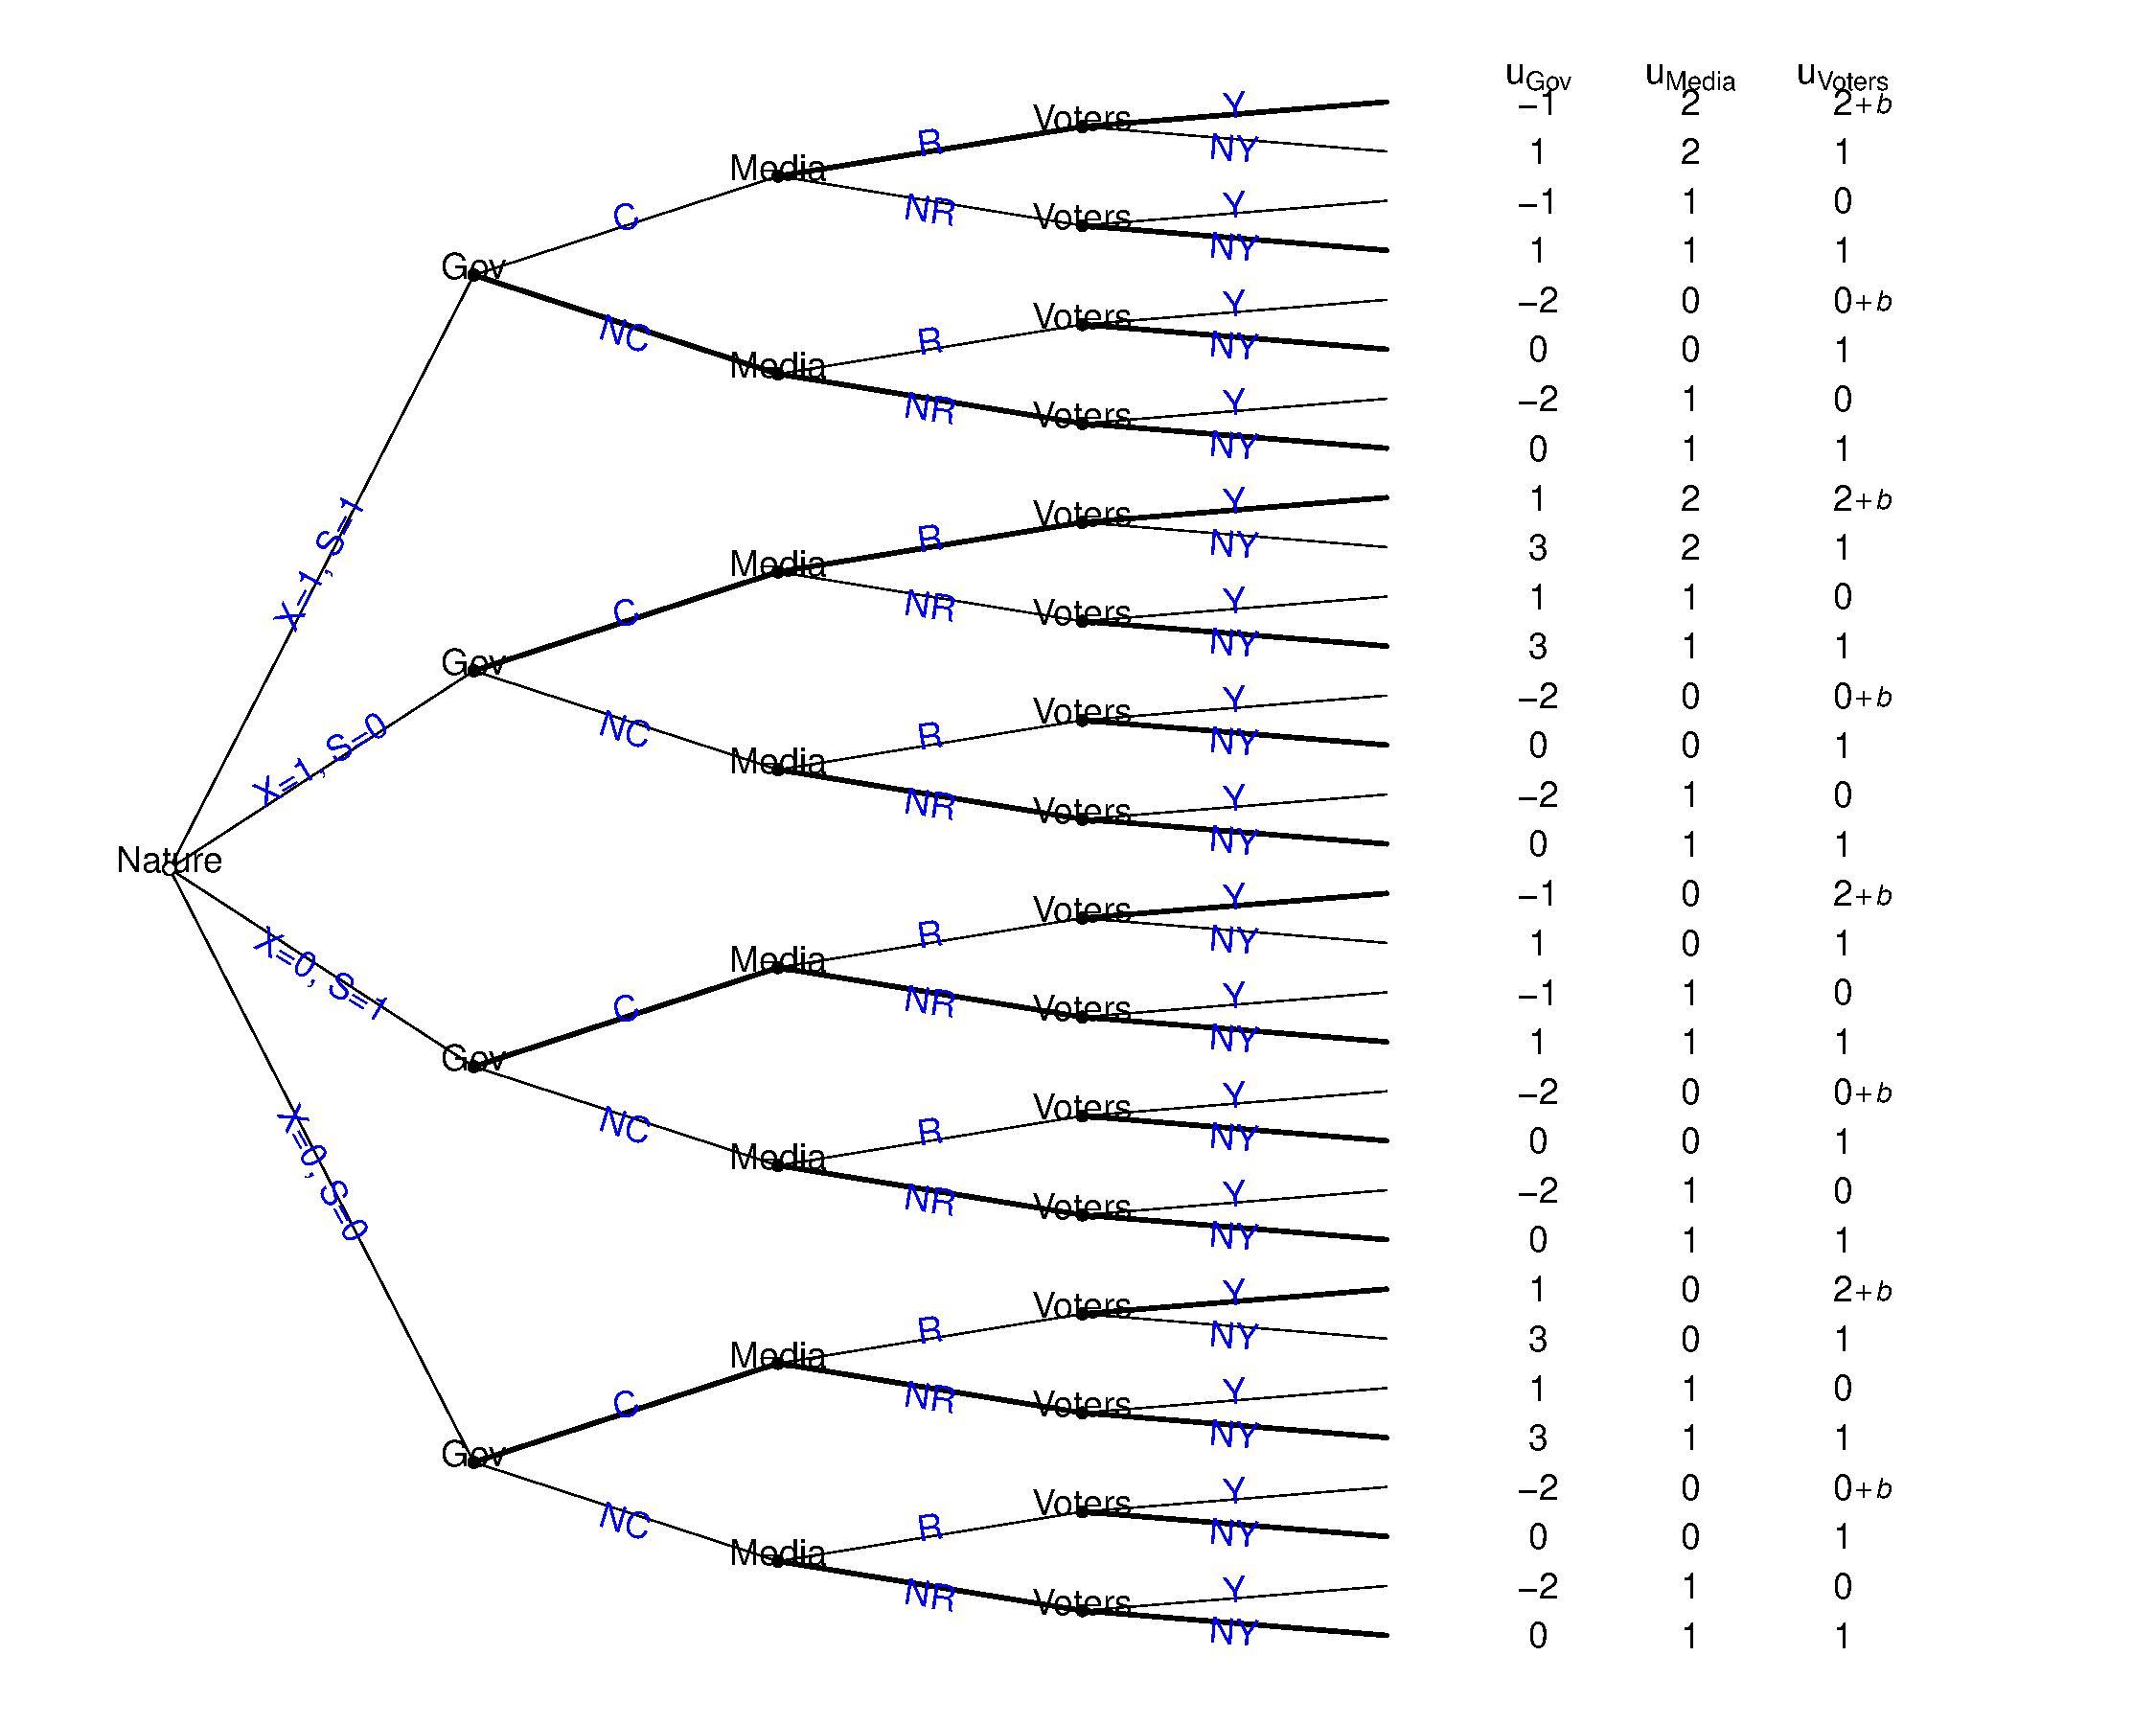
\includegraphics{ii_files/figure-latex/game1-1.pdf}
\caption{\label{fig:game1}\label{fig:tree} A Game Tree. Solid lines represent choices on the (unique) equilibrium path of the subgames starting after nature's move for the case in which \(b=0\).}
\end{figure}

To draw this equilibrium as a DAG we include nodes for every action taken, nodes for features that determine the game being played, and the utilities at the end of the game.

If equilibrium claims are justified by claims about the beliefs of actors then these could also appear as nodes. To be clear however these are not required to represent the game or the equilibrium, though they can capture assumed logics underlying the equilibrium choice. For instance a theorist might claim that humans are wired so that whenever they are playing a ``Stag Hunt'' game they play ``defect.'' The game and this solution can be represented on a DAG without reference to the beliefs of actors about the action of other players. However, if the \emph{justification} for the equilibrium involves optimization given the beliefs of other players, a lower level DAG could represent this by having a node for the game description that points to beliefs about the actions of others, that then points to choices. In a game with dominant strategies, in contrast, there would be no arrows from these beliefs to actions.

For our running example, nodes could usefully include the politician's expectations, since the government's actions depend on expectations of the actions of others. However, given the game there is no gain from including the media's expectations of the voter's actions since in this case the media's actions do not depend on expectations of the voters actions then these expectations should be included.

In Figure \ref{fig:gamedag} we provide two examples of DAGs that illustrate lower level models that support our running example.

The upper graph gives a DAG reflecting equilibrium play in the game described in Figure \ref{fig:tree}. Note that in this game there is an arrow between \(C\) and \(Y\) even though \(Y\) does not depend on \(C\) for some values of \(b\)---this is because conditional independence requires that two variables are independent for \emph{all} values of the conditioning set. For simplicity also we mark \(S\) and \(X\), along with \(b\) as features that affect which subgame is being played---taking the subgames starting after Nature's move. Note that the government's expectations of responses by others matters, but the expectations of other players do not matter given this game and solution. Note that the utilities appear twice in a sense. They appear in the subgame node, as they are part of the definition of the game--though here they are the utilities that players expect at each terminal node; when they appear at the end of the DAG they are the utilities that actually arise (in theory at least).

The lower level DAG is very low and much more general, representing the theory that in three player games of complete information, players engage in backwards induction and choose the actions that they expect to maximize utility given their beliefs about the actions of others. The DAG assumes that players know what game is being played (``Game''), though this could also be included for more fundamental justification of behavioral predictions. Each action is taken as a function of the beliefs about the game, the expectations about the actions of others, and knowledge of play to date. The functional equations---not shown---are given by optimization and belief formation assuming optimization by others.

\begin{figure}

{\centering 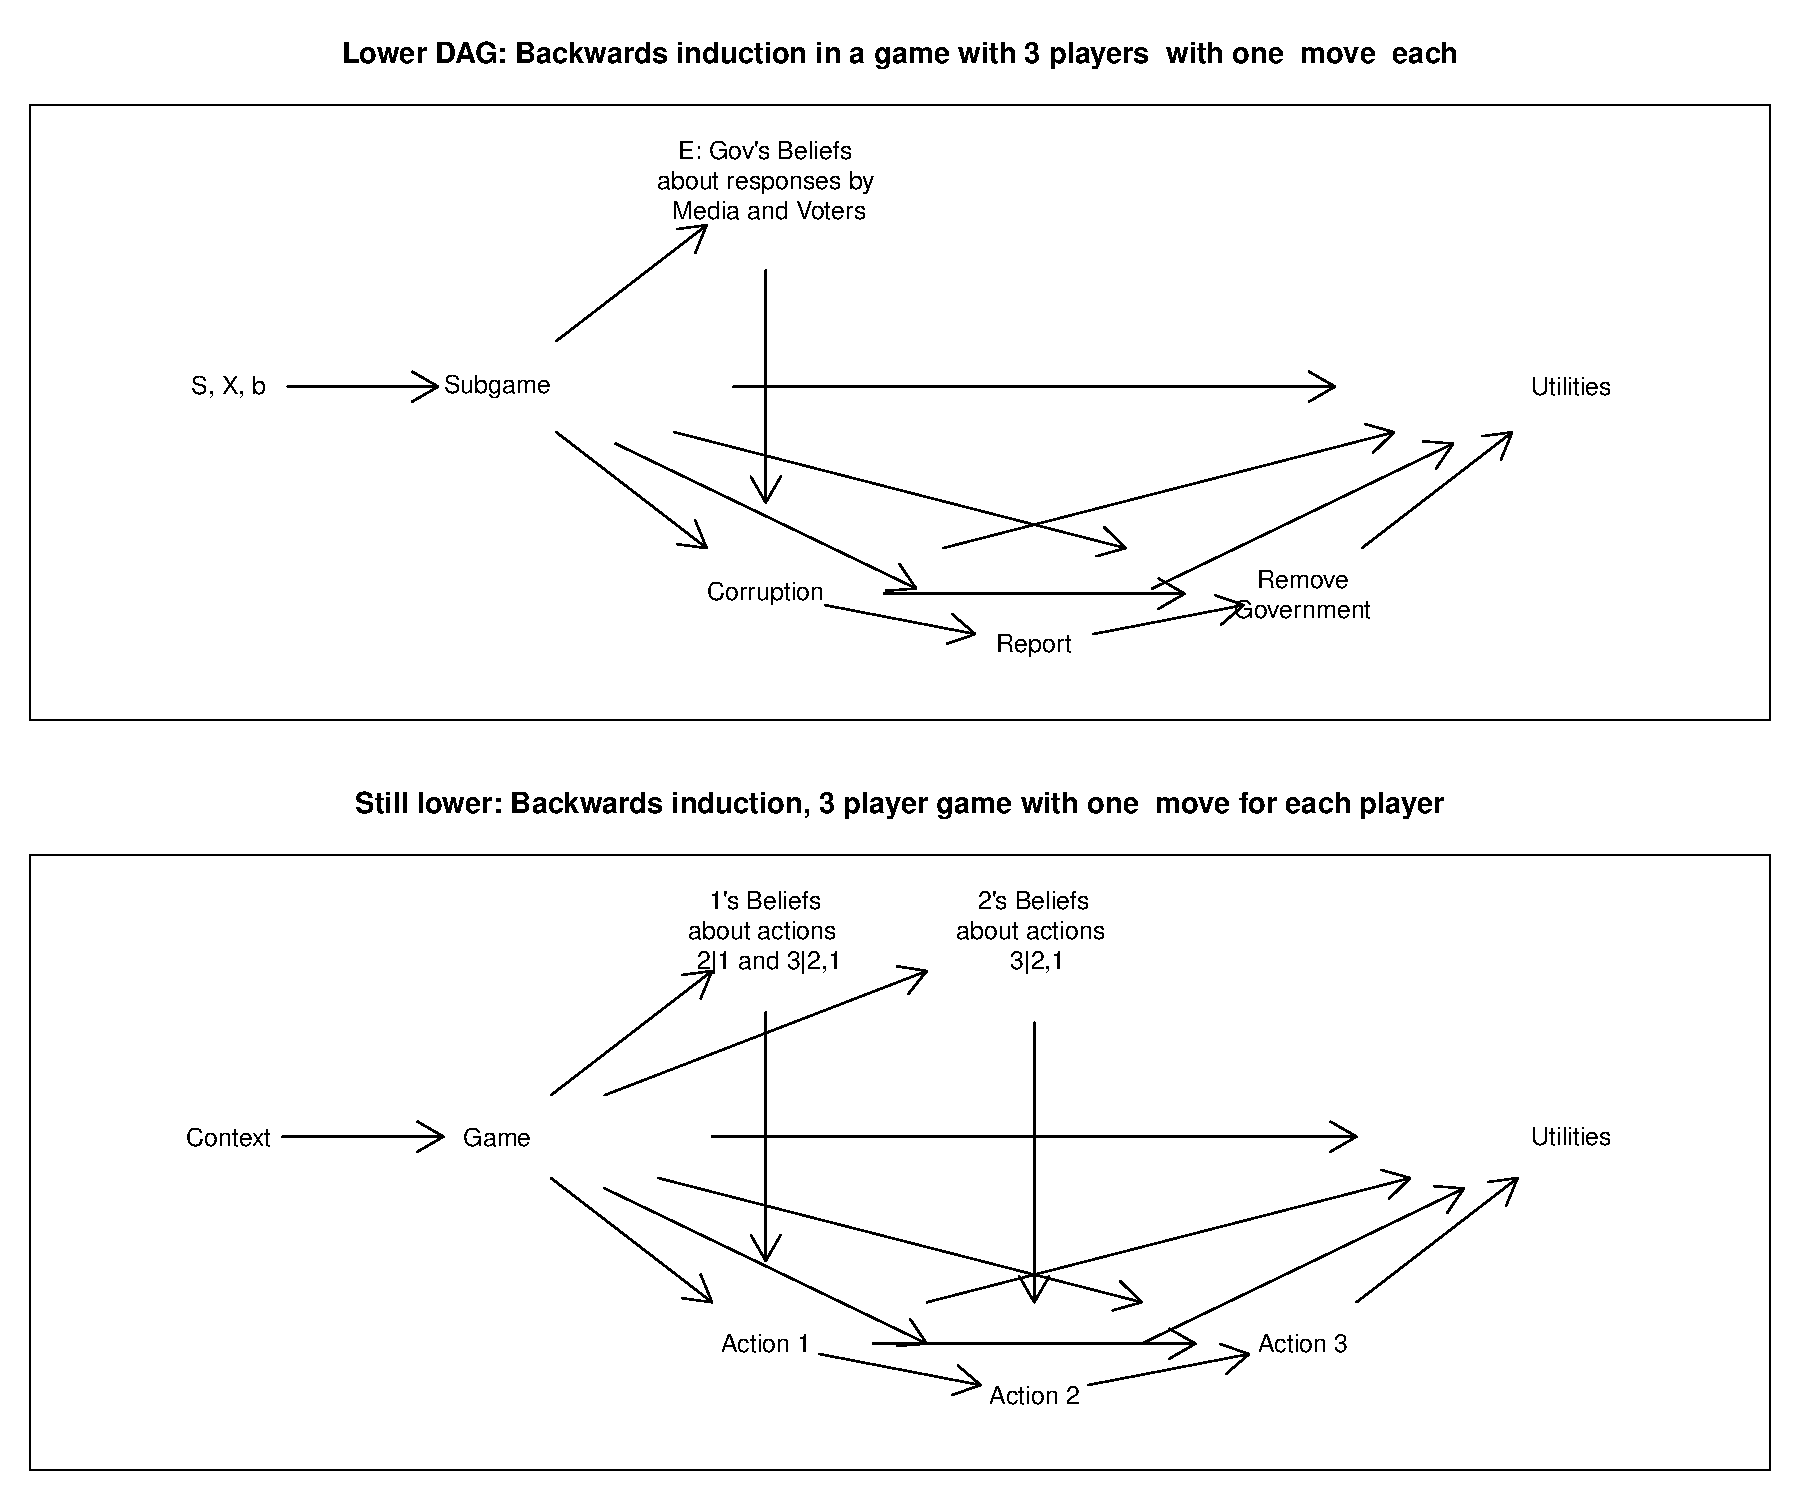
\includegraphics[width=\textwidth]{ii_files/figure-latex/unnamed-chunk-13-1} 

}

\caption{\label{fig:gamedag} The upper panel shows a causal graph that describes  relations between nodes suggested by analysis of  the  game  in Figure \ref{fig:tree} and which can imply the causal graph of  Figure \ref{fig:running}. The game itself  (or beliefs about the game) appear as a node, which are in turn determined by exogneous factors.   The lower panel represents a still lower level and more general theory ``players use backwards induction in three step games of complete information.''}\label{fig:unnamed-chunk-13}
\end{figure}

These lower level graphs can themselves provide clues for assessing relations in the higher level graphs. For instance, the lower level model might specify that the value of \(b\) in the game affects the actions of the government only through their beliefs about the behavior of voters, \(E\). These beliefs may themselves have a stochastic component, \(U_E\). Thus \(b\) high might be thought to reduce the effect of media on corruption. For instance if \(b \in \mathbb{R}_+\), we have \(C= 1-FG(1-\mathbb{1}(b>1))\). If \(X\) is unobserved and one is interested in whether \(S=0\) caused corruption, knowledge of \(b\) is informative. It is a root node in the causal estimand. If \(b>1\) then \(S=0\) did not cause corruption. However if \(b\) matters only because of its effect on \(E\) then the query depends on \(U_E\). In this case, while knowing \(b\) is informative about whether \(S=0\) caused \(C=1\), knowing \(E\) from the lower level graph is more informative.

Note that the model we have examined here involves no terms for \(U_C\), \(U_R\) and \(U_Y\)---that is, shocks to outcomes given action. Yet clearly any of these could exist. One could imagine a version of this game with ``trembling hands,'' such that errors are always made with some small probability, giving rise to a much richer set of predictions. These can be represented in the game tree as moves by nature between actions chosen and outcomes realized. Importantly in a strategic environment such noise could give rise to different types of conditional independence. For instance say that a Free Press only published its report on corruption with probability \(\pi^R\), then with \(\pi^R\) high enough the sensitive government might decide it is worth engaging in corruption even if there is a free press; in this case the arrow from \(X\) to \(C\) would be removed. Interestingly in this case as the error rate rises, \(R\) becomes less likely, meaning that the effect of a \(S\) on \(Y\) becomes gradually weaker (since governments that are not sensitive become more likely to survive) and then drops to 0 as sensitive governments start acting just like nonsensitive governments.

\hypertarget{questions}{%
\chapter{Causal Questions}\label{questions}}

\begin{center}\rule{0.5\linewidth}{\linethickness}\end{center}

Although a lot of empirical work focuses on identifying average causal effects, there is a rich array of other well defined causal questions that can be asked about how variables relate to each other causally. We decribe major families of question and illustrate how these can all be described as questions about the values of nodes in a causal model.

\begin{center}\rule{0.5\linewidth}{\linethickness}\end{center}

The study of causation is central to most empirical social science, whether quantitative analyses of large sets of cases or qualitative, small-\(N\) case studies. Yet a general interest in causality masks tremendous heterogeneity in the kinds of causal questions that scholars tend to ask.

Returning to our inequality and democratization example, we might seek, for instance, to know inequality's average impact on democratization across some set of cases. Alternatively, we might be interested in a particular case---say, Mongolia in 1995---and want to know whether this is a context in which inequality has an effect---a question about causal effects at the case level. Relatedly---but distinctly---we might wonder whether the level of democracy in Mongolia in 1995 is causally attributable to the level of inequality in that case. And we may be interested in \emph{how} causal effects unfold, inquiring about the pathway or mechanism through which inequality affects democratization---a question we can also ask at two levels. We can ask whether inequality affected democratization in Mongolia through mobilization of the masses; and we can ask how commonly inequality affects democratization through mobilization across a broad set of cases.

Rather separate methodological literatures have been devoted to the study of average causal effects, the analysis of case-level causal effects and explanations, and the identification of causal pathways. It is typically understood that their analysis requires quite distinct sets of tools. In this chapter, we take a key integrative step in showing that each of these queries can be readily captured in a causal model. More specifically, we demonstrate how causal queries can be represented as question about one or more \emph{nodes} on a causal graph. When we assimilate our causal questions into a causal model, we are placing what we want to know in formal relation to both what we \emph{already} know and what we can potentially \emph{observe}. As we will see in later chapters, this move allows us then to deploy the model to generate strategies of inference: to determine which observations, if we made them, would be likely to yield the greatest leverage on our query, given our prior knowledge about the way the world works. And by the same logic, once we see the evidence, this integration allows us to ``update'' on our query---figure out in systematic fashion what we \emph{have} learned---in a manner that takes background knowledge into account.

In the remainder of this chapter, we walk through the conceptualization and causal-model interpretation of four key causal queries:

\begin{itemize}
\item
  Case-level causal effects
\item
  Case-level causal attribution
\item
  Case-level explanation
\item
  Average causal effects
\item
  Causal pathways
\end{itemize}

These four are not exhaustive of the causal questions that can be captured in causal graphs, but they are among the more common foci of social scientific investigation.

--\textgreater{}

\hypertarget{causal-queries}{%
\section{Causal queries}\label{causal-queries}}

\hypertarget{case-level-causal-effects}{%
\subsection{Case-level causal effects}\label{case-level-causal-effects}}

The simplest causal question is whether some causal effect operates in an individual case. Does \(X\) have an effect on \(Y\) in this case? For instance, is Yemen in 1995 a case in which a change in economic inequality would produce a change in whether or not the country democratizes? We could put the question more specifically as a query about a causal effect in a particular direction, for instance: Does inequality have a positive effect on democratization in the case of Yemen in 1995?

In counterfactual terms, a query about case-level causation is a question about what would happen if we could manipulate a variable in the case: if we could hypothetically manipulate \(X\)'s value in the case, would \(Y\)'s value also change? To ask whether a positive (or negative) effect operates for a case is to ask whether a particular counterfactual relation holds in that case. If we assume a binary setup for simplicity, to ask whether inequality has a positive effect on democratization is to ask: if we set \(I\) to \(0\) would \(D\) take on a value of \(0\), \emph{and} if we set \(I\) to \(1\), would \(D\) take on a value of \(1\)? (\emph{Both} of these conditions must hold for \(I\) to have a positive effect on \(D\).)

We can easily represent this kind of query in the context of a causal model. We show the DAG for such a model in Figure \ref{fig:casequery}. As introduced in Chapter \ref{theory}, \(\theta^Y\) here represents the causal type characterizing \(Y\)'s response to \(X\) and, if \(X\) and \(Y\) are binary, can take on one of four values: \(\theta^Y_{10}\), \(\theta^Y_{01}\), \(\theta^Y_{00}\), and \(\theta^Y_{11}\) (which map onto our original \(a, b, c\) and \(d\) types). Importantly, given that the value of nodes (or variables) is allowed to vary across cases, this setup allows for \(\theta_Y\)---the causal effect of \(X\) on \(Y\)---to vary across cases. Thus, \(X\) may have a positive effect on \(Y\) in one case (with \(\theta^Y=\theta^Y_{01}\)), \(X\) may have a negative (\(\theta^Y=\theta^Y_{10}\)) or no effect (\(\theta^Y=\theta^Y_{00}\) or \(\theta^Y_{11}\)) on \(Y\) in other cases.

\begin{figure}

{\centering 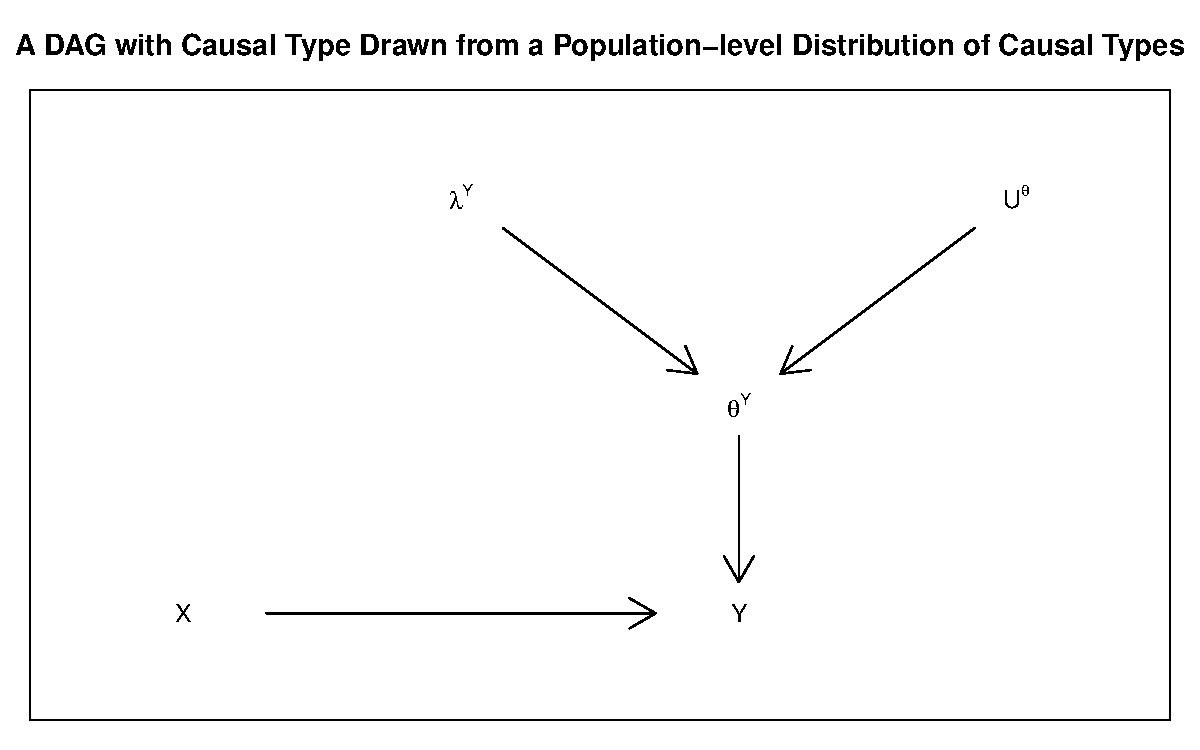
\includegraphics[width=.5\textwidth]{ii_files/figure-latex/unnamed-chunk-15-1} 

}

\caption{\label{fig:casequery} This DAG is a graphical representation of the simple causal setup in which the effect of $X$ on $Y$ in a given case depends on the case's causal type, represented by $\theta^Y$. With a single binary causal variable of interest, we let $\theta_Y$ take on values $\theta^Y_{ij}$, with $i$ representing the value $Y$ takes on if $X=0$ and $j$ representing the value $Y$ takes on if $X=1$. With a binary framework outcome, $\theta^Y$ ranges over the four values: $\theta^Y_{00}$, $\theta^Y_{10}$, $\theta^Y_{01}$ and $\theta^Y_{11}$.}\label{fig:unnamed-chunk-15}
\end{figure}

In this model, then, the query, ``What is \(X\)'s causal effect in this case?'' simply becomes \emph{a question about the value of \(\theta_Y\)}.

Of course, \(\theta_Y\) is not directly observable: causal types are intrinsically unobserved properties of cases. So, as we will see in later chapters, research design becomes a challenge of determining which \emph{observable} nodes in the graph are potentially informative about the unobservable nodes that constitute our causal queries.

\hypertarget{case-level-causal-attribution}{%
\subsection{Case-level causal attribution}\label{case-level-causal-attribution}}

A query about causal attribution is related to, but different from, a query about a case-level causal effect. When asking about \(X\)'s case-level effect, we are asking, ``\emph{Would} a change in \(X\) cause a change in \(Y\) in this case?'' The question of causal attribution is slightly different: ``\emph{Did} \(X\) cause \(Y\) to take on the value it did in this case?'' More precisely, we are asking, ``Given the values that \(X\) and \(Y\) \emph{in fact} took on in this case, would \(Y\)'s value have been different if \(X\)'s value had been different?''

For instance, given that we know that inequality in Taiwan was relatively low and that Taiwan democratized in 1996, was low inequality a \emph{cause} of Taiwan's democratization in 1996? Put differently, given low economic inequality and democratization in Taiwan in 1996, would the outcome in this case have been different if inequality had been high?

This goes beyond simply asking whether Taiwan is a case in which inequality has a causal effect on democratization. Whereas a case-level causal effect is defined in terms of a single \(\theta\) node, we define a causal-attribution query in terms of a larger set of nodes. To attribute \(Y\)'s value in a case to \(X\), we need to know not only whether this is the kind of case in which \(X\) could have an effect on \(Y\) but also whether the context is such that \(X\)'s value \emph{in fact} made a difference.

Consider, for instance, the general setup in Figure \ref{fig:attribquery}. Here, \(Y\) is a function of two variables, \(X\) and \(W\). This means that \(\theta^Y\) is somewhat more complicated than in a setup with one causal variable: \(\theta^Y\) must here define \(Y\)'s response to different combinations of two other variables, \(X\) and \(W\), since \emph{both} of these variables point directly into \(Y\). Thus, \(\theta^Y\) must cover the full set of possible causal interactions between two binary causal variables.

\begin{figure}

{\centering 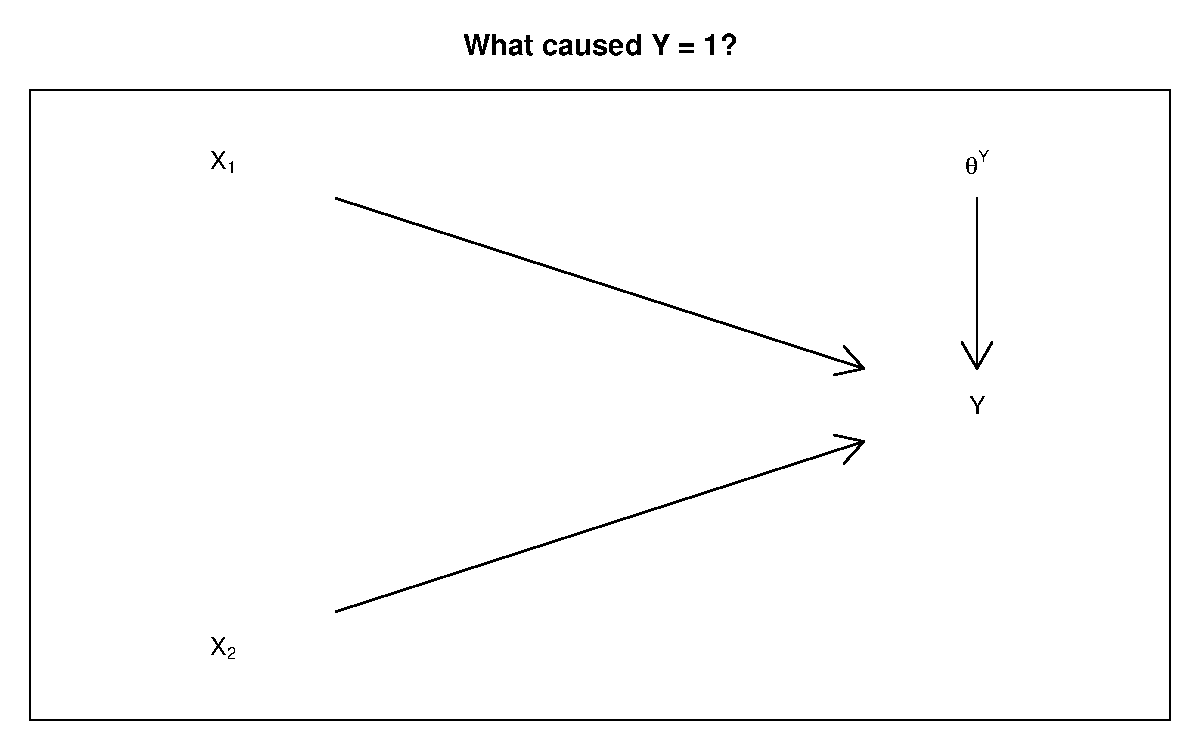
\includegraphics[width=.5\textwidth]{ii_files/figure-latex/attribquery-1} 

}

\caption{This DAG is a graphical representation of the simple causal setup in which $Y$ depends on two variables $X1$ and $X2$. How $Y$ responds to X1 and X2 depnds on $\theta^Y$, the DAG itself does not provide information on whether or how X1 and X2 interact with each other.}\label{fig:attribquery}
\end{figure}

We already saw the set of causal types for a set up like this in Chapter 2 (see Table \ref{tab:PO16}). In the table, there are four column headings representing the four possible combinations of \(X1\) and \(X2\) values. Each row represents one possible pattern of \(Y\) values as \(X1\) and \(X2\) move through their four combinations.

Labelling is a little difficult with so many types. One approach used in Chapter \ref{models}. is to represent change in \(X1\) on the horizontal axis, and change in the second variable, \(X2\), on the vertical axis. The value of \(X1\) increases from 0 to 1 as we move to the \emph{right} (from \(i\) to \(j\) or from \(g\) to \(h\)). And the value of \(X2\) increases from 0 to 1 as we move \emph{up} (from \(i\) to \(g\) or from \(j\) to \(h\)).

One way to conceptualize the size of the causal-type ``space'' is to note that \(X1\) can have any of our four causal effects (the four binary types) on \(Y\) when \(X2=0\); and \(X1\) can have any of four causal effects when \(X2=1\).\footnote{This is precisely equivalent to noting that \(X2\)'s effect on \(Y\) can be of any of the four types when \(X1=0\) and of any of the four types when \(X1=1\).} This yields 16 possible response patterns to combinations of \(X1\) and \(X2\) values.

A query about causal attribution---whether \(X1 = 1\) caused \(Y=1\)--for the modein in Figure \ref{fig:attribquery}, would be defined in terms of both \(X1\) and \(\theta_Y\). Parallel to our Taiwan example, suppose that we have a case in which \(Y=1\) and in which \(X1\) was also 1, and we want to know whether \(X1\) caused \(Y\) to take on the value it did. Answering this question requires knowing whether the case's type is such that \(X1\) would have had a positive causal effect on \(Y\), \emph{given the value of \(X2\)} (which we might think of as the context). Thus, given that we start with knowledge of \(X1\)'s and \(Y\)'s values, our query about causal attribution amounts to a query about two nodes on the graph: (a) the value of \(X2\) and (b) whether the value of \(\theta^Y\) is such that \(X1\) has a positive causal effect given \(X2\)'s value.

Suppose, for instance, that we were to observe \(X2=1\). We then need to ask whether the causal type, \(\theta_Y\), is such that \(X1\) has a positive effect when \(X2=1\). Consider type 8, or \(\theta_{01}^{11}\). This is a causal type in which \(X1\) has a positive effect when \(X2=0\) but no effect when \(X2=1\). Put differently, \(X2=1\) is a sufficient condition for \(Y=1\), meaning that \(X1\) makes no difference to the outcome when \(X2=1\).

In all we have four qualifying types: \(\theta_{00}^{01}\), \(\theta_{01}^{01}\), \(\theta_{10}^{01}\), and \(\theta_{11}^{01}\) (or 2, 4, 10, and 12). In other words, we can attribute a \(Y=1\) outcome to \(X1=1\) when \(X2=1\) and the causal type is one of these four. By parallel reasoning, we can also attribute a \(Y=1\) outcome to \(X1=1\) when \(X2=0\) and the causal type is any of \(\theta_{01}^{00}\), \(\theta_{01}^{01}\), \(\theta_{01}^{10}\), and \(\theta_{01}^{11}\).

Thus, a question about causal attribution is a question about the \emph{joint} value of a set of nodes: about whether the \emph{combination} of context and causal type is such that changing \(X\) would have changed the outcome.

\hypertarget{case-level-explanation}{%
\subsection{Case-level explanation}\label{case-level-explanation}}

So far we have been dealing with causes in the standard counterfactual sense: antecedent conditions a change in which would have produced a different outcome. Sometimes, however, we are interested in identifying antecedent conditions that were not counterfactual difference-makers but that nonetheless \emph{generated} or \emph{produced} the outcome. Consider, for instance, a situation in which an outcome was overdetermined: multiple conditions were present, each of which on their own, \emph{could} have generated the outcome. Then none of these conditions caused the outcome in the counterfactual sense; yet one or more of them may have been distinctively important in \emph{producing} the outcome. The concept of an \emph{actual cause} may be useful in putting a finer point on this kind of causal question.

Let us first approach the concept at an intuitive level. An antecedent condition, \(A\), that played a role in generating an outcome might not be a counterfactual cause because, had it not occurred, some second chain of events set in motion by \(B\) would have unfolded, generating the outcome anyway. In the standard counterfactual scenario, \(A\) is not a counterfactual cause: take away \(A\) and the outcome still happens because of the chain of events emanating from \(B\). Yet let us imagine that the fact that \(A\) \emph{did} occur \emph{prevented} part of \(B\)'s chain of consequences from unfolding and itself producing the outcome. Then let us imagine a tweaked counterfactual comparison in which we \emph{fix} the observed fact that \(B\)'s causal sequence did not fully unfold. We can then ask: \emph{conditional on \(B\)'s sequence not fully unfolding}, would \(A\) have been a counterfactual cause of the outcome? If so, then we say that \(A\) is an ``actual cause''" of the outcome. We have, in a sense, identified \(A\) as distinctively important in the production of the outcome, even if it was not a case-level cause in the usual sense.

More formally, and using the definition provided by \citep{halpern2015modification}, building on \citep{halpern2005causesa} and others, we say that a condition (\(X\) taking on some value \(x\)) was an \emph{actual cause} of an outcome (of \(Y\) taking on some value \(y\)), where \(x\) and \(y\) may be collections of events, if:

\begin{enumerate}
\def\labelenumi{\arabic{enumi}.}
\tightlist
\item
  \(X=x\) and \(Y=y\) both happened
\item
  there is some set of variables, \(\mathcal W\), such that if they were fixed at the levels that they actually took in the case, and if \(X\) were to be changed, then \(Y\) would change (where \(\mathcal W\) can also be an empty set)
\item
  no strict subset of \(X\) satisfies 1 and 2 (there is no redundant part of the condition, \(X=x\))
\end{enumerate}

The definition thus describes a condition that \emph{would} have been a counterfactual cause of the outcome if we were to imagine holding constant some set of events that in fact occurred (and that, in reality, might not have been constant if the actual cause had not in fact occurred).

A motivating example used in much of the literature on actual causes \citep[e.g.~][]{hall2004two} imagines two characters, Sally and Billy, simultaneously throwing stones at a bottle. Both are great shots and hit whatever they aim at. Sally's stone hits first, and so the bottle breaks. However, Billy's stone \emph{would} have hit had Sally's not hit, and would have broken the bottle. Did Sally's throw cause the bottle to break? Did Billy's?

By the usual definition of causal effects, neither Sally's nor Billy's action had a causal effect: without either throw, the bottle would still have broken. We commonly encounter similar situations in the social world. We observe, for instance, the onset of an economic crisis and the breakout of war---either of which would be sufficient to cause the government's downfall---but with the economic crisis occurring first and toppling the government before the war could do so. Yet neither economic crisis nor war made a difference to the outcome.

To return to the bottle example, while neither Sally's nor Billy's throw is a counterfactual cause, there is an important sense in which Sally's action obviously broke the bottle, and Billy's did not. This intuition is confirmed by applying the definition above. Consider first the question: Did Sally's throw break the bottle? Conditions 1 and 3 are easily satisfied, since Sally \emph{did} throw and the bottle \emph{did} break (Condition 1), and ``Sally threw'' has no strict subsets (Condition 3).

Condition 2 is met if Sally's throw made a difference, counterfactually speaking; and in determining this, we are permitted to condition on (to fix in the counterfactual comparison) any event or set of events that actually happened (or on on none at all). To see why Condition 2 is satisfied, we have to think of there being three steps in the process: Sally and Billy throw, Sally's or Billy's rock hits the bottle, and the bottle breaks. In actuality, Billy's stone did not hit the bottle. And conditioning on this actually occurring event (Billy's stone not hitting), the bottle would \emph{not} have broken had Sally not thrown. From the perspective of counterfactual causation, it may seem odd to condition on Billy's stone not hitting the bottle when thinking about Sally not throwing the stone since Sally's throwing the stone was the very thing that prevented Billy from hitting the bottle. Yet Halpern argues that this is an acceptable thought experiment for establishing the importance of Sally's throw since conditioning is constrained to the actual facts of the case. Moreover, the same logic shows why Billy is not an actual cause. The reason is that Billy's throw is only a cause in those conditions in which Sally did not hit the bottle. But because Sally \emph{did} actually hit the bottle, we are not permitted to condition on Sally not hitting the bottle in determining actual causation. We thus cannot---even through conditioning on actually occurring events---construct any counterfactual comparison in which Billy's throw is a counterfactual cause of the bottle's breaking.

The striking result here is that there can be grounds to claim that a condition was the actual cause of an outcome even though, under the counterfactual definition, the effect of that condition on the outcome is 0. (At the same time, all counterfactual causes are automatically actual causes; they meet Condition 2 by conditioning on nothing at all, an empty set \(\mathcal W\).) One immediate methodological implication follows: since actual causes need not be causes, there are risks in research designs that seek to understand causal effects by tracing back actual causes---i.e., the way things actually happened. If we traced back from the breaking of the bottle, we might be tempted to identify Sally's throw as the cause of the outcome. We would be right only in an actual-causal sense, but wrong in the standard, counterfactual causal sense. Chains of events that appear to ``generate'' an outcome are not always causes. \footnote{Perhaps more surprising, it is possible that the expected causal effect is negative but that \(X\) is an actual cause in expectation. For instance, say that 10\% of the time Sally's shot intercepted Billy's shot but without hitting the bottle. In that case the average causal effect of Sally's throw on bottle breaking is \(-0.1\) yet 90\% of the time Sally's throw is an actual cause of bottle breaking (and 10\% of the time it is an actual cause of non-breaking). For related discussions see \citet{menzies1989probabilistic}.}

As with other causal queries, the question ``Was \(X=x\) the actual cause of \(Y=y\)?'' can be redefined as a question about which values for exogenous nodes produce conditions under which \(X\) could have made a difference. To see how, let us run through the Billy and Sally example again, but formally in terms of a model. Consider Figure \ref{fig:actualquery}, where we represent Sally's throw (\(S\)), Billy's throw (\(B\)), Sally's rock hitting the bottle (\(H^S\)), Billy's rock hitting the bottle (\(H^B\)), and the bottle cracking (\(C\)). Each endogenous variable has a \(\theta\) term associated with it, capturing its response to its parents. We capture the possible ``preemption'' effect with the arrow pointing from \(H^S\) to \(H^B\), allowing that whether Sally's rock hits to affect whether Billy's rock hits.

Let us again imagine that Sally threw (\(S=1\)), Billy threw (\(B=1\)), and the bottle cracked (\(C=1\)). Let us say that \(\theta^{H^B}\) takes on a value such that (a) \(H^B=0\) whenever \(H^S=1\) (Sally's hit preempts Billy's) and (b) \(B\) has a positive effect on \(H^B\) when \(H^S=0\) (Billy's throw hits if Sally's doesn't). Further, assume that \(S\) has a positive effect on \(H^S\). Let us finally posit that \(\theta^C\) takes on a value such that \(C=1\) if \(H^B\) equals \(1\).\footnote{That is, \(\theta^C\) equals some value \(\theta_{ij}^{11}\), where \(H^S\) operates along the horizontal axis and \(H^B\) along the vertical and \(i\) and \(j\) can be any 0 or 1 values.} This is a set of \(\theta\) values under which the query, ``Does \(S\) have a causal effect on \(C\)?'' must be answered in the negative. Similarly, this is a context in which \(C=1\) cannot be causally attributed to \(S=1\). If Sally had not thrown, then Sally's rock would not have hit the bottle, which means that Billy's rock would have hit, and the bottle would still have cracked---still, \(C=1\).

However, it is still possible that \(S=1\) was an actual cause of \(C=1\). To complete this query, we need to ask whether there is some node value that we can hold fixed at the value that it \emph{actually} assumed in the case such that \(S\) would have a causal effect on the outcome. Fixing \(B=1\) (Billy throws) cannot help (since if Billy throws, Billy hits, and the bottle cracks anyway). However, under \(S=1\) and \(B=1\), given the \(\theta\) values we have posited, \(H^B=0\): Billy's rock does not hit. If we hold constant that \(H^B=0\), then there is an ``opportunity'' for \(S\) to matter in that \(C\) is no longer forced to 1 (by Billy's rock hitting). But for \(S\) to matter under his scenario, something else has to be true: \(\theta^C\)'s value must allow for \(H^S\) to have a positive effect on \(C\) when \(H^B=0\).

Using our two-cause notation (with \(H^S\) on the horizontal axis, and \(H^B\) on the vertical), and given that we have already stipulated that \(C=1\) when \(H^B=1\), the one permissible value for \(\theta^C\) is \(\theta^{11}_{01}\). This is causal type in which neither \(H^B\) nor \(H^S\) can be causal if both Billy and Sally throw: whenever one variable is 1, the other has no effect. But it is also a type in which each has a causal effect if the other is held at 0.

It is also the case, as we have said, that all counterfactual causes are actual causes. They are, quite simply, counterfactual causes when we hold \emph{nothing} fixed (\(\mathcal W\) is the empty set). Thus, in fact, any \(\theta^S\), \(\theta^{H^S}\) and \(\theta^C\) values in which \(S\) has a positive effect when \(B=1\) will do. This includes, for instance, a \(\theta^C\) value in which Billy's hitting has no effect on the bottle (perhaps Billy doesn't throw hard enough!): e.g., \(\theta^{01}_{01}\). Here, Sally's throw is both a counterfactual cause and an actual cause of the bottle's cracking. The larger point is that actual cause queries can, like all other causal queries, be defined as questions about the values of nodes in a causal model.

\begin{figure}

{\centering 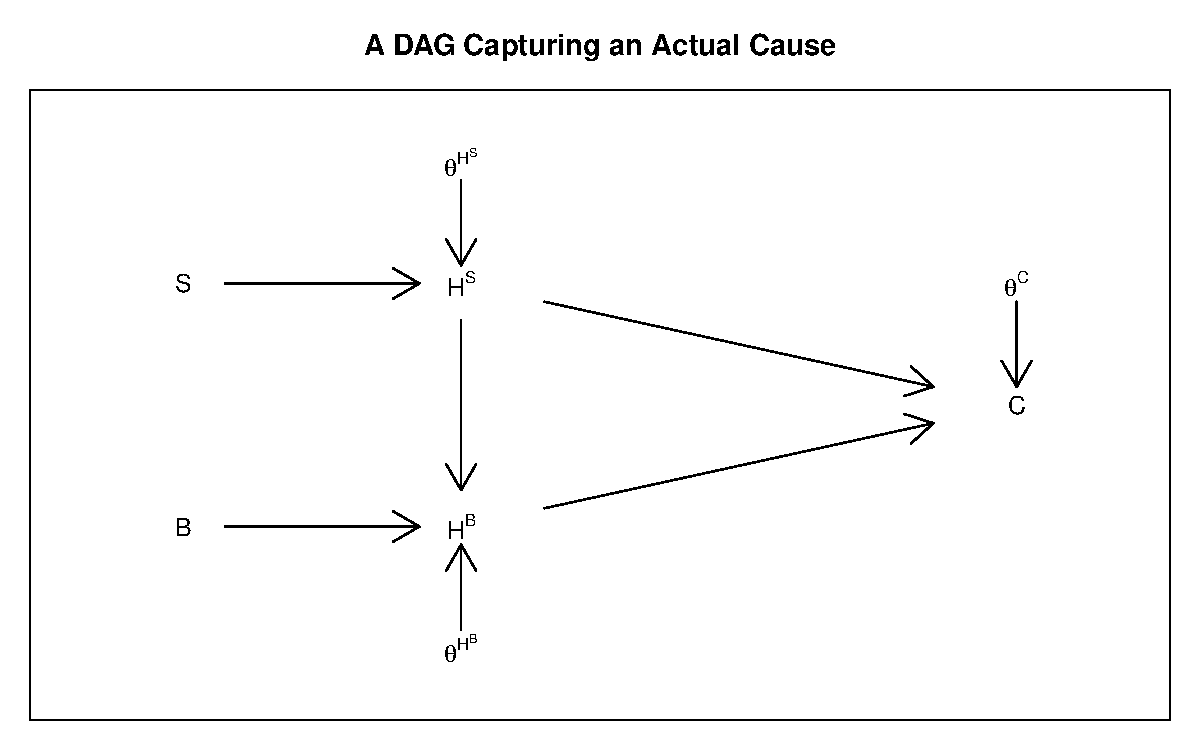
\includegraphics[width=.5\textwidth]{ii_files/figure-latex/unnamed-chunk-16-1} 

}

\caption{\label{fig:actualquery} This DAG is a graphical representation of the simple causal setup in which the effect of $X$ on $Y$ in a given case depends on the case's causal type, represented by $\theta^Y$. With a single binary causal variable of interest, we let $\theta_Y$ take on values $\theta^Y_{ij}$, with $i$ representing the value $Y$ takes on if $X=0$ and $j$ representing the value $Y$ takes on if $X=1$. With a binary framework outcome, $\theta^Y$ ranges over the four values: $\theta^Y_{00}$, $\theta^Y_{10}$, $\theta^Y_{01}$ and $\theta^Y_{11}$.}\label{fig:unnamed-chunk-16}
\end{figure}

Actual causes are conceptually useful whenever there are two sufficient causes for an outcome, but one preempts the operation of the other. For instance, we might posit that both the United States' development of the atomic bomb was a sufficient condition for U.S. victory over Japan in World War II, and that U.S. conventional military superiority was also a sufficient condition and would have operated via a land invasion of Japan. Neither condition was a counterfactual cause of the outcome because both were present. However, holding constant the \emph{absence} of a land invasion, the atomic bomb was a difference-maker, rendering it an actual cause. The concept of actual cause thus helps capture the sense in which the atomic bomb contributed to the outcome, even if it was not a counterfactual cause.

Similarly, the question of how \emph{common} it is for a condition to be an actual cause can be expressed as values of nodes, possibly including nodes that record parameter values for the relevant exogenous nodes.

An extended notion \citep[p 81]{halpern2016actual} of actual causes restricts the imagined counterfactual deviations to states that are more likely to arise (more ``normal'') than the factual state. We will call this notion a `'notable cause.'' Similarly, one cause, \(A\), is ``more notable'' than another cause, \(B\), if a deviation in \(A\) from its realized state is (believed to be) more likely than a deviation in \(B\) from its realized state.

For intuition, we might wonder why a Republican was elected to the presidency in a given election. In looking at some minimal winning coalition of states that voted Republican, we might distinguish between a set of states that \emph{always} vote Republican and a set of states that usually go Democratic but voted Republican this time. If the coalition is minimal winning, then every state that voted Republican is a cause of the outcome in the standard (difference making) sense. However, only the states that usually vote Democratic are notable causes since it is only for them that the counterfactual scenario (voting Democratic) was more likely to arise than the factual scenario. In a sense, we take the ``red'' states' votes for the Republican as given---placing it, as it were, in the causal background---and identify as ``notable'' those conditions that mattered and easily could have gone differently. By the same token, we can say that, among those states that voted Republican this time, those that more commonly vote Democratic are \emph{more} notable causes than those that less commonly vote Democratic.

Again, whether something is a notable cause, or the likelihood in some population that a condition is a notable cause, can be expressed as a claim about the value of a set of root nodes.

Though not a focus of our applied examples we show formally how to estimate these estimands in the Appendix, section XXX.

\hypertarget{average-causal-effects}{%
\subsection{Average causal effects}\label{average-causal-effects}}

A more general query asks about an average causal effect in some population. In counterfactual terms, a question about average causal effects is: if we manipulated the value of \(X\) for all cases in the population---first setting \(X\) to one value for all cases, then changing it to another value for all cases---by how much would the average value of \(Y\) in the population change? Like other causal queries, a query about an average causal effect can be conceptualized as learning about a node in a causal model.

We can do this by conceiving of any given case as being a member of a population composed of different causal types. When we seek to estimate an average causal effect, we seek information about the \emph{shares} of these causal types in the population.

More formally and adapted from \citet{humphreys2015mixing}, we can use \(\lambda^Y_{ij}\) to refer to the \emph{share} of cases in a population that has causal type \(\theta^Y_{ij}\). Thus, given our four causal types above, \(\lambda^Y_{10}\) is the proportion of cases in the population with negative effects; \(\lambda_{01}\) is the proportion of cases with positive effects; and so on. We can, of course, also think of these shares as probabilities; that is, we can think of any given case as being ``drawn'' from a multinomial distribution with probabilities \(\lambda = (\lambda^Y_{10}, \lambda^Y_{01}, \lambda^Y_{00}, \lambda^Y_{11})\). One nice feature of this setup, with both \(X\) and \(Y\) as binary, the average causal effect can be simply characterized as the share of positive-effect cases less the share of negative-effect cases: \(\lambda^Y_{01} - \lambda^Y_{10}\).

Graphically, we can represent this setup by including \(\lambda^Y\) in a more complex causal graph as in Figure \ref{fig:DAGace}. As in our setup for case-level causal effects, \(X\)'s effect on \(Y\) in a case depends on (and only on) the case's causal type, \(\theta^Y\). The key difference is that we now model the case's type not as exogenously given, but as a function of two additional variables: the distribution of causal types in a population and a random process through which the case's type is ``drawn'' from that distribution. We represent the type distribution as \(\lambda^Y\) (a vector of values for the proportions \(\lambda^Y_{10}, \lambda^Y_{01}, \lambda^Y_{00}, \lambda^Y_{11}\)) and the random process drawing a \(\theta^Y\) value from that distribution as \(U_\theta\).

In this model, our causal query---about \(X\)'s average causal effect---is thus defined by the vector \(\lambda^Y\), and specifically by the shares of negative- and positive-causal-effect cases, respectively, in the population. What is \(X\)'s average effect on \(Y\) amounts to asking: what are the values of \(\lambda^Y_{10}\) and \(\lambda^Y_{01}\)? As with \(\theta^Y\), \(\lambda^Y\) is not directly observable. And so the empirical challenge is to figure out what we \emph{can} observe that would allow us to learn about \(\lambda^Y\)'s component values?\footnote{Note also that \(\lambda^Y\) can be thought of as itself drawn from a distribution, such as a Dirichlet. The hyperparameters of this underlying distribution of \(\lambda\) would then represent our uncertainty over \(\lambda\) and hence over average causal effects in the population.}

\begin{figure}

{\centering 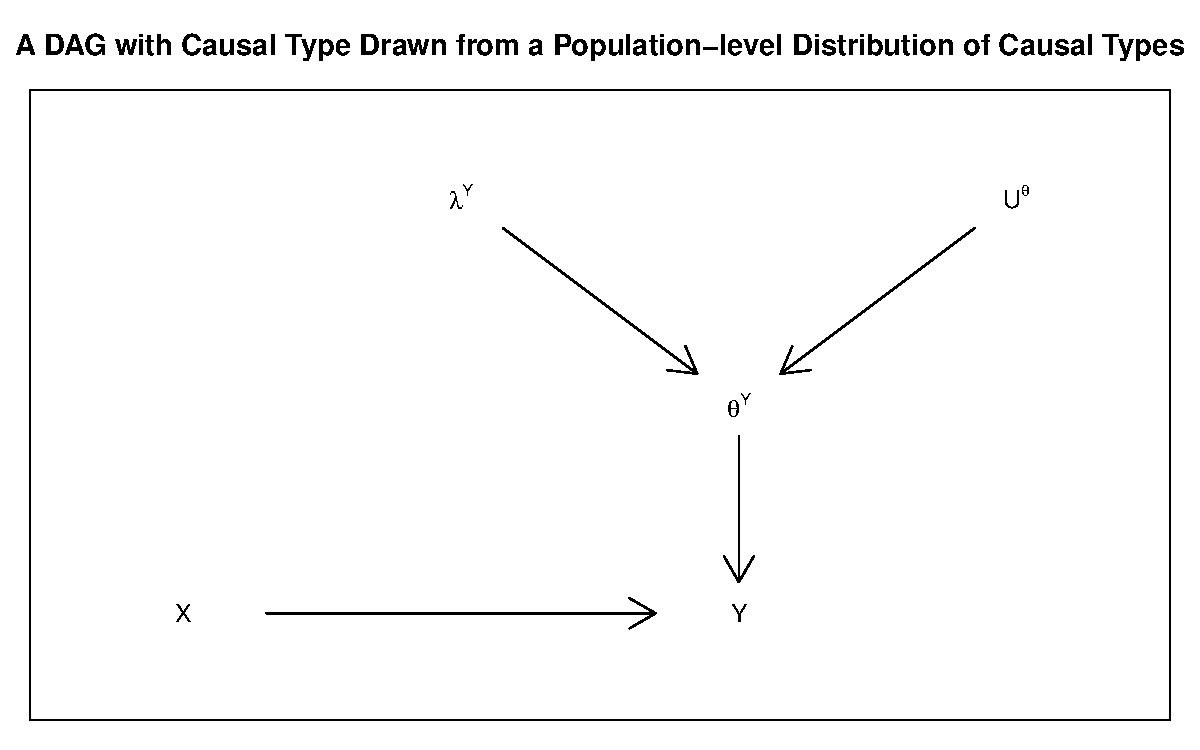
\includegraphics[width=.5\textwidth]{ii_files/figure-latex/unnamed-chunk-17-1} 

}

\caption{\label{fig:DAGace} This DAG is a graphical representation of a causal setup in which cases are drawn from a population composed of different causal types. As before, $X$'s effect on $Y$ is a function of a causal-type variable, $\theta^Y$. Yet here we explicitly model the process through which the case's type is drawn from a distribution of types in a population. The variable $\lambda$ is a vector representing the multinomial distribution of causal types in the population while $U_\theta$ is a random variable representing the draw of each case from the distribution defined by $\lambda$. A case's causal type, $\theta^Y$, is thus a joint function of $\lambda^Y$ and $U^{\theta_Y}$.}\label{fig:unnamed-chunk-17}
\end{figure}

We can, of course, likewise pose queries about other population-level causal quantities. For instance, we could ask for what proportion of cases in the population \(X\) has a positive effect: this would be equivalent to asking the value of \(\lambda^Y_{01}\), one element of the \(\lambda^Y\) vector. Or we could ask about the proportion of cases in which \(X\) has no effect, which would be asking about \(\lambda^Y_{00} + \lambda^Y_{11}\).

\hypertarget{causal-paths}{%
\subsection{Causal Paths}\label{causal-paths}}

To develop richer causal understandings, researchers often seek to describe the causal path or paths through which effects propagate. Consider the DAG in Figure \ref{fig:DAGpaths}, in which \(X\) can affect \(Y\) through two possible pathways: directly and via \(M\). Assume again that all variables are binary, taking on values of \(0\) or \(1\). As we have seen in Chapter \ref{theory}, mediation models require causal-type nodes that point into any mediators as well as into the outcome variable. So here we have drawn in a causal-type variable defining \(M\)'s response to \(X\), \(\theta^M\), and a causal-type variable capturing \(Y\)'s response, \(\theta^Y\). Importantly, \(\theta^Y\) defines \(Y\)'s response to \emph{two} parent variables: \(M\) and \(X\).

Suppose that we observe \(X=1\) and \(Y=1\) in a case. Suppose, further, that we have reasonable confidence that \(X\) has had a positive effect on \(Y\) in this case. We may nonetheless be interested in knowing whether that causal effect ran \emph{through} \(M\). We will refer to this as a query about a causal path. A causal path query, of course, goes beyond assessing whether some mediating event along the path occurred. We cannot, for instance, establish that the top path in Figure \ref{fig:DAGpaths} was operative simply by determining the value of \(M\) in this case---though that will likely be useful information.

Rather, the question of whether the top (mediated) causal path is operative is a composite question of two parts: First, does \(X\) have an effect on \(M\) in this case? Second, does that effect---the difference in \(M\)'s value caused by a change in \(X\)---in turn \emph{cause} a change in \(Y\)'s value? In other words, what we want to know is whether the effect of \(X\) on \(Y\) depends on---\emph{will not operate without}---the effect of \(X\) on \(M\).\footnote{A very similar question is taken up in work on mediation where the focus goes to understanding quantities such as the ``indirect effect''" of \(X\) on \(Y\) via \(M\). Formally, the indirect effect would be \[Y(X=1, M = M(X=1,\theta^M), 
  \theta^Y) - Y(X = 1, M = M(X=0, \theta^M), \theta^Y))\], which captures the difference to \(Y\) if \(M\) were to change in the way that it would change due to a change in \(X\), but without an actual change in \(X\) \citep[ p 132, \citet{imai2010general}]{pearl2009causality}.} Framing the query in this way makes clear that asking whether a causal effect operated via a given path is in fact asking about a specific set of causal effects lying along that path.

\begin{figure}

{\centering 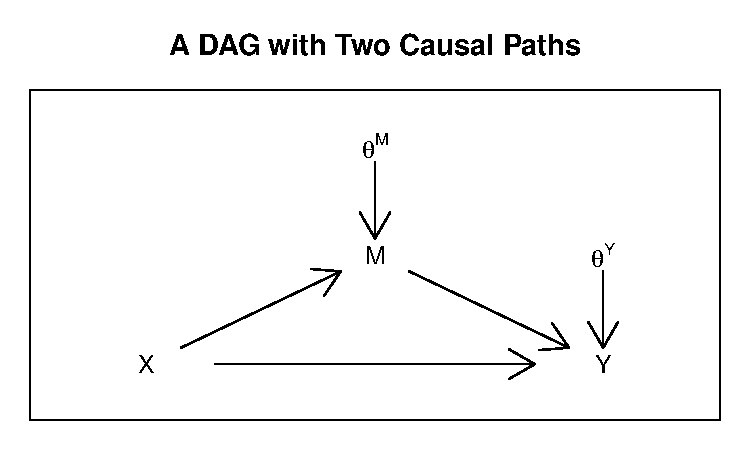
\includegraphics[width=.5\textwidth]{ii_files/figure-latex/unnamed-chunk-18-1} 

}

\caption{\label{fig:DAGpaths} Here $X$ has effects on $Y$ both indirectly through $M$ and directly.}\label{fig:unnamed-chunk-18}
\end{figure}

As we can show, we can also define a causal-path query as a question about specific nodes on a causal graph. In particular, just as we have defined other questions about causal effects in terms of causal-type nodes, a causal path can also be defined in terms of the values of type nodes: specifically, in the present example, in terms of the nodes \(\theta^M\) and \(theta^Y\). To see why, let us first note that there are two combinations of effects that would allow \(X\)'s positive effect on \(Y\) to operate via \(M\): (1) \(X\) has a positive effect on \(M\), which in turn has a positive effect on \(Y\); or (2) \(X\) has a negative effect on \(M\), which has a negative effect on \(Y\).

Thus, in establishing whether \(X\) affects \(Y\) through \(M\), the first question is whether \(X\) affects \(M\) in this case. Whether or not it does is a question about the value of the causal-type node, \(\theta^M\). Let us assume that \(\theta^M\) can take on four possible values corresponding to the four possible responses to \(X\): \(\theta^M_{10}, \theta^M_{01}, \theta^M_{00}, \theta^M_{11}\).\footnote{In other words, \(X\)'s effect on \(M\) could be negative, positive, absent with \(M\) stuck at \(0\), or absent with \(M\) stuck at \(1\), respectively.} For sequence (1) to operate, \(\theta^M\) must take on the value \(\theta^M_{01}\), representing a positive effect of \(X\) on \(M\). For sequence (2) to operate, \(\theta^M\) must take on the value \(\theta^M_{10}\), representing a negative effect of \(X\) on \(M\).

\(\theta^Y\), as for our causal-attribution example, defines \(Y\)'s response to different combinations of two other variables---here, \(X\) and \(M\)---since \emph{both} of these variables point directly into \(Y\). Another way to think about this setup is that \(M\) is not just a possible mediator of \(X\)'s indirect effect; \(M\) is also a potential \emph{moderator} of \(X\)'s direct effect. Where \(X\) can have both an mediated effect through \(M\) and a direct effect, \(X\) and \(M\) also potentially \emph{interact} in affecting \(Y\).

This results in sixteeen possible values for \(\theta^Y\)---again as shown above in Table \ref{tab:PO16}.

What values of \(\theta^Y\)
then are compatible with the operation of the \(M\) causal path? Let us first consider this question with respect to sequence (1), in which \(X\) has a positive effect on \(M\), and that positive effect is necessary for \(X\)'s positive effect on \(Y\) to occur. For this sequence to operate, \(\theta^M\) must take on the value of \(\theta^M_{01}\). When it comes to \(\theta^Y\), then, what we need to look for types in which \(X\)'s effect on \(Y\) \emph{depends on \(M\)'s taking on the value it does as a result of \(X\)'s positive effect on \(M\)}.

We are thus looking for causal types that represent two kinds of counterfactual causal relations operating on nodes. First, \(X\) must have a positive effect on \(Y\) when \(M\) changes as it should given \(X\)'s positive effect on \(M\). Second, that change in \(M\), generated by a change in \(X\), must be \emph{necessary} for \(X\)'s positive effect on \(Y\) to operate. The thought experiment here thus imagines a situation in which \(X\) changes from \(0\) to \(1\),\footnote{This is the natural thought experiment when explaining a case with realized value of \(X=1\), in which the outcome can be thought of as having been generated by a change from \(X=0\). The identification of types does hinge, however, on the direction in which we imagine types changing. In other situations, we might observe \(X=Y=0\) and thus conceive of the outcome as having been generated by a change from \(X=1\) to \(X=0\) (again, assuming a positive effect of \(X\) on \(Y\)). When we do this, query 2 below changes: we are now looking for types in which \(Y=1\) when \(X=0\) but \(M=1\). (Does \(Y\) stay at \(1\) when \(X\) moves to \(0\) but \(M\) doesn't?) The queries are then satisfied by types \(6\) and \(8\), rather than \(2\) and \(6\).} but \(M\) does \emph{not} change to the value that it should as a result of this change in \(X\). We then inspect our types to see if \(Y\) would change from \(0\) to \(1\) in this situation. It is this counterfactual that isolates the causal significance of the path that runs through \(M\). It is only if \(Y\) would \emph{not} change to \(1\) in this situation that we have identified a causal-type for which the \(M\)-mediated path matters.

Assuming a positive effect of \(X\) on \(M\) (\(\theta^M=\theta^M_{01}\)), we thus need to apply three queries to \(\theta^Y\):\footnote{Using standard potential outcomes notation, we can express the overall query, conditioning on a positive effect of \(X\) on \(M\), via the inequality \(Y(1, M(1)) - Y(0, M(0)) > Y(1, M(0)) - Y(0, M(0))\). The three specific queries formulated below simply correspond to the three unique elements of this expression. We can also readily map the path query that we are defining here---does the positive effect of \(X\) on \(Y\) depend on \(X\)'s effect on \(M\)---onto a query posed in terms of indirect effects. For instance, in our binary setup, conditioning our path query on a positive causal effect of \(X\) on \(Y\), a positive effect of \(X\) on \(M\), and an imagined change from \(X=0\) to \(X=1\) generates precisely the same result (identifies the same \(\theta^Y\) types) as asking which \(\theta^Y\) types are consistent with a positive indirect effect of \(X\) on \(Y\), conditioning on a positive total effect and \(X=1\).}

\begin{enumerate}
\def\labelenumi{\arabic{enumi}.}
\item
  Is \(X=1\) a counterfactual cause of \(Y=1\)? Establishing this positive effect of \(X\) involves two queries:

  \begin{enumerate}
  \def\labelenumii{\alph{enumii})}
  \item
    Where \(X=0\), does \(Y=0\)? As we are assuming \(X\) has a positive effect on \(M\), if \(X=0\) then \(M=0\) as well. We thus look down the \(X=0, M=0\) column and eliminate those types in which we do not observe \(Y=0\). This eliminates types \(9\) through \(16\).
  \item
    Where \(X=1\), does \(Y=1\)? Again, given \(X\)'s assumed positive effect on \(M\), \(M=1\) under this condition. Looking down the \(X=1, M=1\) column, we eliminate those types where we do not see \(Y=1\). We retain only types \(2, 4, 6,\) and \(8\).
  \end{enumerate}
\item
  Is \(X\)'s effect on \(M\) necessary for \(X\)'s positive effect on \(Y\)? That is, do we see \(Y=1\) \emph{only} if \(M\) takes on the value that \(X=1\) generates (\(M=1\))? To determine this, we inspect the \emph{counterfactual} condition in which \(X=1\) yet \(M=0\), and we ask: does \(Y=0\)? Of the four remaining types, only \(2\) and \(6\) pass this test.
\end{enumerate}

Under these and only these two values of \(\theta^Y\)---\(\theta_{00}^{01}\) and \(\theta_{00}^{11}\)---we will see a positive effect of \(X\) on \(Y\) for which the \(M\)-mediated path is causally necessary as long as \(X\) also has a positive effect on \(M\). These two \(\theta^Y\) values are also different from one another in an interesting way. For type \(\theta_{00}^{11}\), \(X\)'s effect on \(Y\) runs strictly through \(M\): if \(M\) were to change from \(0\) to \(1\) \emph{without} \(X\) changing, \(Y\) would still change from \(0\) to \(1\). \(X\) is causally important for \(Y\) \emph{only} insofar as it affects \(M\). In a case of type \(\theta_{00}^{11}\), then, anything else that similarly affects \(M\) would generate the same effect on \(Y\) as \(X\) does. In type \(\theta_{00}^{01}\), however, both \(X\)'s change to \(1\) \emph{and} the resulting change in \(M\) are necessary to generate \(Y\)'s change to \(1\); \(X\)'s causal effect thus requires both the mediated and the unmediated pathway. Andhere \(X\) itself matters in the counterfactual sense; for a case of type \(\theta_{00}^{01}\), some other cause of \(M\) would \emph{not} generate the same effect on \(Y\).

We can undertake the same exercise for sequence (2), in which \(X\) first has a negative effect on \(M\), or \(\theta^M=\theta^M_{10}\). Here we adjust the three queries for \(\theta^Y\) to take account of this negative effect. Thus, we adjust query 1a so that we are looking for \(Y=0\) when \(X=0\) and \(M=1\). In query 1b, we look for \(Y=1\) when \(X=1\) and \(M=0\). And for query 2, we want types in which \(Y\) fails to shift to \(1\) when \(X\) shifts to \(1\) but \(M\) stays at \(1\). Types \(\theta_{01}^{00}\) and \(\theta_{11}^{00}\) pass these three tests.

In sum, we can define a query about causal paths as a query about the value of \(\theta\) terms on the causal graph. For the graph in Figure \ref{fig:DAGpaths}, asking whether \(X\)'s effect runs via the \(M\)-mediated path is asking whether one of four combinations of \(\theta^M\) and \(\theta^Y\) hold in case:

\begin{itemize}
\tightlist
\item
  \(\theta^M=\theta^M_{01}\) and (\(\theta^Y=\theta_{00}^{01}\) or \(\theta_{00}^{11}\))
\item
  \(\theta^M=\theta^M_{01}\) and (\(\theta^Y=\theta_{01}^{00}\) or \(\theta_{11}^{00}\))
\end{itemize}

It is worth noting how different this formulation of the task of identifying causal pathways is from widespread understandings of process tracing. Scholars commonly characterize process tracing as a method in which we determine whether a mechanism was operating by establishing whether the events lying along that path occurred. As a causal-model framework makes clear, finding out that \(M=1\) (or \(M=0\), for that matter) does not establish what was going on causally. Observing this intervening step does not by itself tell us what value \(M\) \emph{would} have taken on if \(X\) had taken on a different value, or whether this would have changed \(Y\)'s value. We need instead to conceive of the problem of identifying pathways as one of figuring out the \emph{counterfactual} response patterns of the variables along the causal chain. As we will demonstrate later in the book, explicitly characterizing those response patterns as nodes in a causal model helps us think systematically about empirical strategies for drawing the relevant inferences.

\hypertarget{illustration-with-the-running-example}{%
\section{Illustration with the Running Example}\label{illustration-with-the-running-example}}

We can more fully illustrate the definition of causal queries in terms of exogenous nodes on a graph by thinking through their application to the simple causal model described in Chapter 2.

We illustrate the model again in figure \ref{fig:running2}.

\begin{figure}

{\centering 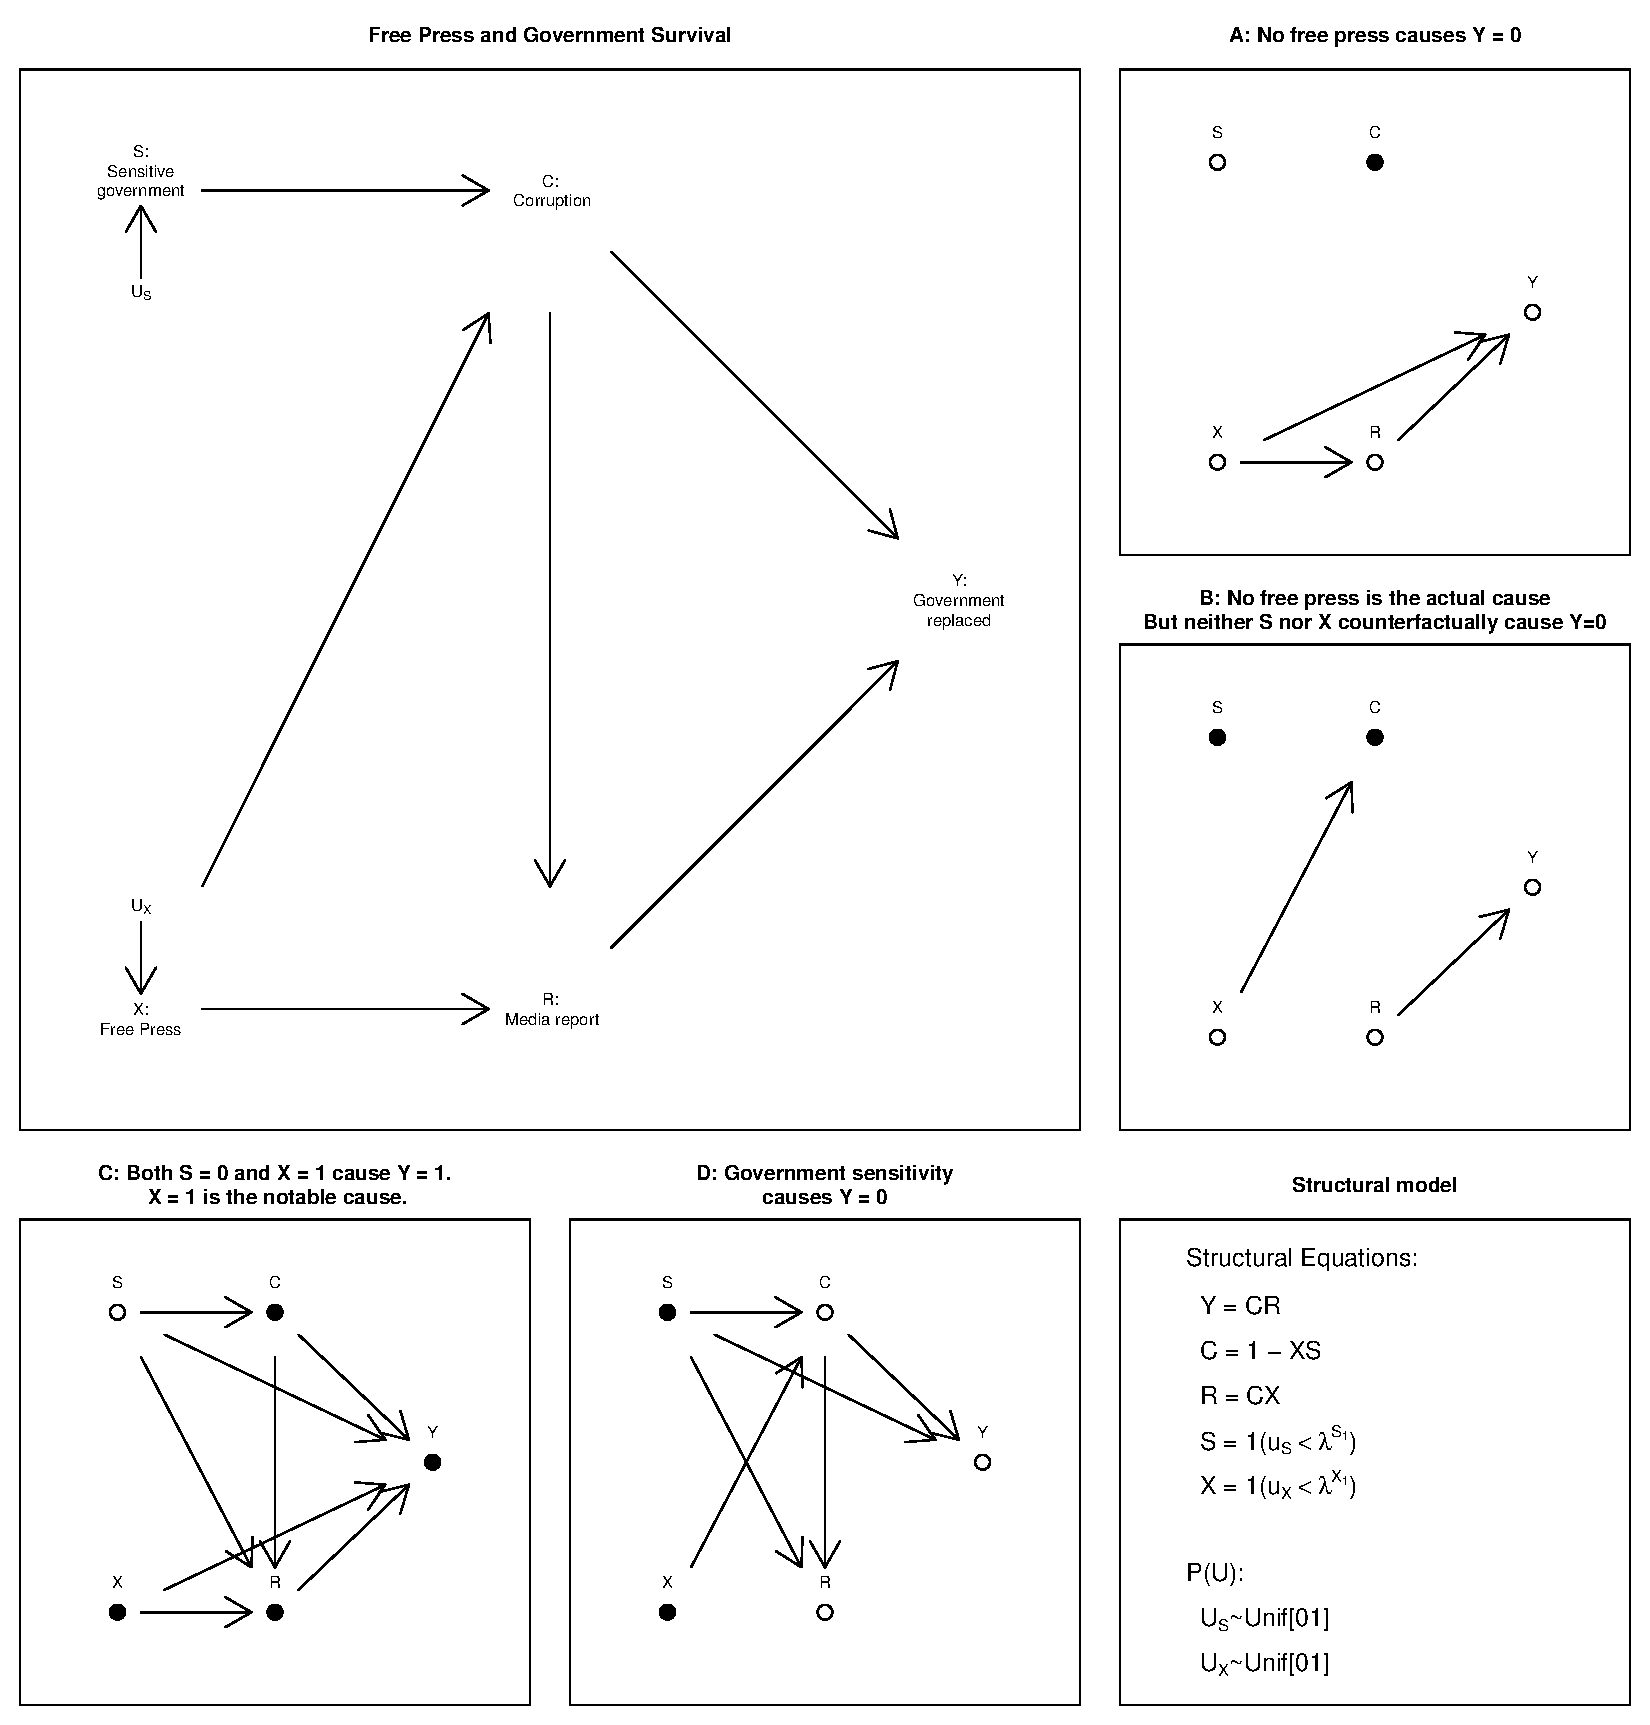
\includegraphics[width=\textwidth]{ii_files/figure-latex/running2-1} 

}

\caption{The main panel shows a simple causal model. $S$ and $X$ are stochastic, other variables determined by their parents, as shown in bottom right panel. Other panels show four possible histories that can arise depending on values taken by $S$ and $X$, along with causal relations in each case. The equations for $S$ and $X$ are written with indicator variables, which take a value of 1 whenever the $u$ value is less than the $\lambda$ value.}\label{fig:running2}
\end{figure}

THe main panel here is the same as in Chapter 2 but but now we add in a set of another four panels. In these panels we leave the \(\lambda\) and \(U\) terms implicit as they will not come into play in our analysis of these graphs. In these four panels, we show all possible `'realizations'' of the graph given the four possible contexts defined by the exogenous nodes, \(S\) and \(X\). We build each of the four possible by assessing outcomes and counterfactual relationships for each possible combination of \(S\) and \(X\) values. A hollow circle at a node indicates that the variable takes on a value of \(0\) while a shaded circle indicates a value of \(1\). The arrows indicate causal effects. More specifically, an arrow pointing from one variable to another indicates that a manipulation of the first variable would cause a change in the second variable, \emph{given the values realized by all other variables that are not the first variable's descendants}. Unlike in a conventional DAG, we represent here both the direct effect of each variable on its child and each variable's indirect (mediated) causal effects on its descendants. As we can see from the various arrows in the panels, we can use a single, simple causal model to think through a wide range of causal relationships that might be of interest.\footnote{Though similar, these graphs are not DAGS or natural beams (or submodels). The panels reflect outcomes conditional on the values of \(S\) and \(X\), but they are not themselves DAGs because they indicate the values taken by nodes and include arrows between two nodes when and only when one causes the other, directly or indirectly. To construct ``natural beams'' \citep[ 10.3]{pearl2009causality}, we fix a realization of root variables, \(U\), (here, \(\mathcal U = (S, X)\)); then for each variable, \(V_i\) we partition \(pa(V_i)\) into a set of ``engaged parents,'' \(S\), and ``disengaged parents,'' with the property that (a) \(f_i(S(u), \overline{s}, u) = V_i(u)\) for \emph{all} values of \(\overline{s}\) and (b) \(f_i(s', \overline{S}(u), u) \neq V_i(u)\) for \emph{some} \(s'\). Thus a natural beam would connect a parent to a child if, given the particular history, the parent mattered for the child's outcome.} Since the values of all variables in a model are determined by the values of the exogenous nodes, this is equivalent to saying that the arrows show the causal effects that are operating each \emph{context.}

One important feature of DAGs is immediately evident from a comparison of the DAG with subgraphs \(A, B, C\), and \(D\) in the figure. Consistent with the rules of DAG-construction, the DAG includes arrows between all variables that are under any circumstances directly causally related; but the inclusion of an arrow does not mean that two variables are \emph{always} causally related. For instance, while the DAG (large graph) has an arrow running from \(X\) to \(R\), we can see from the subgraphs (where we deviate from the standard grammar of DAGs) that the causal effect is contingent on context: it is present only when \(S=0\) (panels \(A\) and \(C\)) but not when \(S=1\). The arrows in a DAG represent dependencies that exist under \emph{some}, but not necessarily under all, values of the exogenous variables.

These five graphs allow us to define all causal claims of interest. The graphs illustrate, in other words, how causal queries can be represented as the value of the exogenous nodes in a causal diagram. Let us consider each causal query in turn.

\textbf{Case-level causal effect.} Working with the four subgraphs, we can show that the query, ``What is the effect of one variable on another in this case?'' is equivalent to asking about the values of the model's exogenous variables, \(X\) and \(S\). Consider, for instance, the query: Do media reports of corruption, \(R\), have a causal effect on government removal from office, \(Y\), in this case? Turning to the subgraphs, we can simply ask in which of these four graphs---in which context---\(R\) has a causal effect on \(Y\): where is there an arrow running from \(R\) to \(Y\)?\footnote{The subgraphs are derived from application of Equation EQUATION REFERENCE. We can work through the \(R \rightarrow Y\) relationship to demonstrate how this is done. Consider the effect of \(R\) on \(Y\) given \(S=0, X=0\). This is the arrow between \(R\) and \(Y\) in panel \(A\). Removing the arrows pointing to \(R\), the distribution over nodes when \(R=r'\) is: \(P(c,y | \hat{r}=r', s =0, x=0)\). We are interested in \(P(y=1| \hat{r}=1, s =0, x=0) - P(y=1 | \hat{r}= 0, s =0, x=0)\). The second term is easy as for all cases in which \(r=0\), \(y=0\); and so \(P(y=1|| \hat{r}= 0)=0\). We focus then on \(P(y=1| \hat{r}=1, s= 0, x= 0)\). Taking the marginal distribution, this can be written \(\sum_{c=0}^1P(y=1|r=1, c)P(c|s=0,x=0)\). From the structural equations, we know that \(P(c=1|s=0,x=0)=1\) and that \(P(y=1|r=1, c=1)=1\). So the marginal distribution is \(P(y=1| \hat{r}=1, s= 0, x= 0) = 1\); and the treatment effect of \(R\) on \(Y\), conditional on the characteristics of this case, is then 1. This positive effect is represented with the arrow from the \(R=0\) node to the \(Y=0\) node in panel \(A\).} We can readily see that \(R\) has an effect---a positive effect---on \(Y\) in all configurations of exogenous node values (i.e., in all subgraphs) except when \(X=1\) and \(S=1\) (panel \(D\)); the absence of an arrow in panel \(D\) indicates that \(R\)'s effect on \(Y\) is 0 in that context. Thus, given our model, asking whether there is a case-level causal effect of \(X\) on \(Y\) is equivalent to asking whether either \(S\) or \(X\) or both are equal to \(0\) in the case.

Another way to put the point is that \(S\) and \(X\) jointly determine a case's causal type when it comes to the effect of \(R\) on \(Y\). Returning to our four causal types, the graphs tell us that a case is a \(b\) type (positive effect) with respect to the \(R \rightarrow Y\) relationship whenever at least one of \(S\) or \(X\) is \(0\). If \(S=X=1\), then a case is a \(c\) type (no effect, with the outcome fixed at \(Y=0\)).

We can work through other relationships in the model similarly. For instance, does a free press have an effect on government removal in a case? See an \(X\)-to-\(Y\) arrow only in panels \(A\) and \(C\), we can thus conclude that \(X\) has a causal effect on \(Y\) in (and only in) cases in which \(S=0\).

For now, we are simply using the models to \emph{define} a query about a case-level causal effect. This definition sets the stage for our discussion of research design---how one might go about empirically addressing this query---later in the book. We can point the way toward that discussion by noting making two broad points. If the presence of a free press and government's sensitivity to public opinion are observable, then estimating case-level causal effects will simply be a matter of measuring these two exogenous nodes (or, for some queries, just one of them). However, we will often be in a situation in which the nodes defining our causal query are not observable. Our models of the world often include concepts that are theoretically central to a causal logic but cannot be directly measured. Consider, for instance, government sensitivity to public opinion. When a model's exogenous variables are unobservable, then our research design may require using information from other, \emph{observable} nodes to draw inferences about context. This is a key strategy of process tracing that we develop in later chapters.

\textbf{Average causal effects.} Average causal effects are simply averages of case-level causal effects for the population. Since case-level causal effects are determined by the values of the exogenous nodes in cases, we need to average over the distribution of case-level contexts in the population. Put differently, the average causal effect of any variable on another will depends on how commonly the relevant case-level conditions---those in which the causal effect is and is not present---occur. In our current example, we have seen that the free press makes a difference to government survival if and only if the government is \emph{non-sensitive} (panels \(A\) and \(C\)): the non-sensitive government gets exposed as corrupt if and only if there is a free press while the sensitive government never gets replaced because it adjusts to the presence of a free press by eliminating corruption. Similarly, the sensitivity of the government (and the resulting level of corruption) matters only if there \emph{is} a free press (panels \(C\) and \(D\)). Without a free press, non-sensitive and, thus, corrupt governments do not get exposed and so stay on; with a free press, non-sensitive (and, thus, corrupt) governments get replaced.

Thus, the \emph{average} effect of each of these initial causes on the outcome will depend on the probability with which the other cause is absent or present. To define a query about average causal effects, we need to examine the full probabilistic causal model as graphed in the large panel in Figure \ref{fig:running2}. What is the average causal effect of a free press (\(X\)) on government removal (\(Y\))? As we have learned from the subgraphs, this effect is fully defined by the value of \(S\). In particular, the effect of \(X\) on \(Y\) is equal to \(1\) when \(S=0\), and is equal to \(0\) when \(S=1\). As we've noted, we calculate the average causal effect by averaging causal effects over the distribution of the relevant exogenous variables -- which, here, is only \(S\). In the probabilistic model, \(S\) is a function of \(\lambda^S\) and \(U_S\). In particular, \(S=1\) whenever \(u_S < \lambda^S\). Since \(U_S\) has a uniform distribution, this simply means that \(S=1\) with probability \(\lambda_1^S\); likewise, \(S=0\) with probability \(1-\lambda_1^S\). Thus, we calculate \(X\)'s average causal effect on \(Y\) by multiplying each causal effect by the probability of \(S\)'s taking on the value that generates that effect: \(1 \times (1-\lambda_1^S) + 0 \times \lambda_1^S = 1-\lambda_1^S\). Put differently, the causal effect of a free press on government removal is equal to the commonness of insensitive governments in the relevant population of cases.

We have thus defined our causal query in terms of an exogenous variable, \(\lambda_1^S\), in the probabilistic causal model. Note that, just as \(S\) acts as a causal-type variable for \(X\)'s effect on \(Y\), querying \(\lambda_1^S\) is equivalent to asking about the distribution of causal types in the population. In our four-type framework, cases with \(S=0\) are \(b\) (positive effect) types with respect to the \(X \rightarrow Y\) relationship; cases with \(S=1\) are \(c\) types (no effect, \(Y=0\)). (There are, here, no \(a\) or \(d\) types.) Thus, \(\lambda_1^S\) represents the share of \(c\) types and \(1-\lambda_1^S\) the share of \(b\) types in the population, vis-a-vis \(X\)'s effect on \(Y\).

We can follow the same procedure for all causal relationships in the model. Returning, for instance, to the effect of \(R\) on \(Y\), we learned from the subgraphs that \(R\) has a causal effect of \(1\) in panels \(A,B\) and \(C\)---that is, whenever it is not the case that \(X=1\) and \(S=1\)---and otherwise of \(0\). Thus, the \(R\)'s average causal effect is the weighted average \(1 \times (1-\lambda_1^S \times \lambda_1^X) + 0 \times \lambda_1^S \times \lambda_1^X\) = \(1-\lambda_1^S \times \lambda_1^X\). This is simply the probability of not having both \(X=1\) and \(S=1\). Here, then, we have defined the causal query in terms of two exogenous nodes in the probabilistic model, \(\lambda_1^S\) and \(\lambda_1^X\). \footnote{Likewise, the average causal effect of \(R\) conditional on \(S=1\) is \(1-\lambda_1^X\) (the probability of ending up in panel B, rather than D); and the average causal effect of \(R\) given \(S=0\) is 1 (since it has an effect in both panels A and C).}

\textbf{TO BECOME A LONG FOOTNOTE\ldots{}}
These quantities can be calculated from the distributions in the same way as we calculated the case-level effects. Removing the arrows pointing to \(R\), the distribution over nodes when \(R=r'\)---but this time not fixing \(S\) and \(X\)---is \(P(s,x,c,y | \hat{r}=r')\). Again the key part is \(P(y=1| \hat{r}=1)\), which can be written \(\sum_x\sum_s\sum_c P(x)P(s)P(c|x,s)P(y|c, r= 1)\). Using the structural equations, this simplifies to \(\sum_x\sum_s P(x)P(s)P(c=1|x,s) = P(x=0)P(s=0) + P(x=0)P(s=1) + P(x=1)P(s=0)\), or, \(1-\lambda_1^S\lambda_1^X\).

In the same way, we can construct the average treatment effect for each of the exogenous variables:

\begin{itemize}
\tightlist
\item
  \(\tau_X = E_S(Y(X=1|S)-Y(X=0|S)) = -(1-\lambda_1^S)\)
\item
  \(\tau_S = E_X(Y(S=1|X)-Y(S=0|X)) = \lambda_1^X\){]}
  \textbf{LONG FOOTNOTE ENDING HERE}
\end{itemize}

In general, then, we can define queries about average causal effects as queries about the exogenous nodes that represent a causal model's probabilistic components. In the present example, probabilistic components enter only as determinants of the initial substantive causal variables. In other models, variables further downstream might also have stochastic components, a query about average causal effects might include thus further exogenous terms representing population-level distributions. Estimating average causal effects thus amounts drawing inferences about these nodes.\footnote{Given the model, data will be useful for estimating average effects only if one is uncertain about the distributions of \(S\) and \(X\), which are a function of \(U_S\) and \(\lambda_1^S\) and \(U_X\) and \(\lambda_1^X\), respectively. In this example \(\lambda_1^S\) and \(\lambda_1^X\) are fixed in the model and so we do not learn anything about them from data. If however \(\lambda_1^S\) and \(\lambda_1^X\) are represented as nodes that are themselves produced by some other distribution -- such as a Beta distribution --- then the question of understanding average effects is the question of making inferences about these nodes.}

\textbf{Actual cause.} Returning to a case-level query, the concept of an actual cause becomes useful when outcomes are overdetermined. Suppose there is a case with a sensitive government (\(S=1\)) and no free press (\(X=0\)), as in panel B. Then the \emph{survival} of the government is over-determined: neither government sensitivity nor the free press is a counterfactual cause. (A lack of a free press is enough for even a corrupt government to survive; and sensitivity ensures non-corruption and, thus, survival even in the presence of a free press.)

Nevertheless, we can distinguish between the causes in terms of which one was an actual cause. Conditioning on there being corruption, which there actually was, the lack of a free press \emph{is} a counterfactual cause of government survival: if there had been a free press, holding corruption constant, then the government would have been removed. This makes the lack of a free press an actual cause---that is, a counterfactual cause when some (or no) feature of what actually happened is kept fixed. However, there is no set of realized variable values that we can condition on to make the presence of a sensitive government a counterfactual cause; thus, it is not an actual cause.

The context---the values of the exogenous nodes in the subgraphs, \(S\) and \(X\)---determines which variables will be actual causes through setting the realized values of all endogenous variables in the model and thus restricting the values on which conditioning is permitted for the determination of actual causes. Since corruption \emph{is} present whenever \(S=1\) and \(X=0\), we are permitted in this context to condition on its presence, and the free press is an actual cause of government retention. In contrast, the sensitivity of the government is not an actual cause in this same context. Given no free press, there will always be corruption but no reporting on corruption, which makes government removal impossible, regardless of government sensitivity; thus, there is no subset of actual events that, when kept fixed, would make a change to a non-sensitive government result in the government's fall. In sum, asking whether a variable in a model was the actual cause of an outcome can equivalently be understood as asking about the values of the model's exogenous nodes. Answering that question will consist either of directly observing those exogenous conditions or drawing inferences about them from other, observable nodes.

\textbf{Notable cause.} In the event that that there is a non-sensitive government (\(S=0\)) and a free press (\(X=1\)), as in panel \(C\), the government gets replaced and \emph{both} of the two causes matter counterfactually for government replacement. (Absent either one, the government would survive.) Again, however, we can distinguish between them, this time on the basis of notable causation. The question, for identifying a notable cause, is how commonly the causal variable in question takes on its realized, as opposed to a counterfactual, value. Thus, like average causal effects, notable causation depends on \emph{population-level} distributions---in the present example, on the parameters \(\lambda_1^S\) and \(\lambda_1^X\). If, for instance, governments are more frequently sensitive (the counterfactual) than non-sensitive (the actual value)---i.e., \(\lambda_1^S > 0.5\)---then the non-sensitive government is a notable cause. However, if free presses are rarer than non-sensitive governments---i.e.~\(\lambda_1^X < 1-\lambda_1^S\)---then the free press is a \emph{more} notable cause than the non-sensitive government.

\textbf{Causal Paths.} Note finally that different causal paths can give rise to the same outcome, where the different paths can be distinguished based on values of root nodes \(S\) and \(X\). For example, the government may be retained (\(Y=0\)) because there is no free press (\(X=0\)) and so no negative reporting on the government, regardless of the value of \(S\); or because, there is a free press (\(X=1\)) and a sensitive government (\(S=1\)) takes account of this and does not engage in corruption. \textbf{\color{red} To be improved to link more closely to our abstract discussion of paths as estimands.}

\hypertarget{bayeschapter}{%
\chapter{Bayesian Answers}\label{bayeschapter}}

\begin{center}\rule{0.5\linewidth}{\linethickness}\end{center}

We run through the logic of Bayesian updating and show how it is used for answering queries of interest. We illustrate with applications to correlational and process tracing inferences.

\begin{center}\rule{0.5\linewidth}{\linethickness}\end{center}

Bayesian methods are just sets of procedures to figure out how to update beliefs in light of new information.

We begin with a prior belief about the probability that a hypothesis is true. New data then allow us to form a posterior belief about the probability of the hypothesis. Bayesian inference takes into account the consistency of the evidence with a hypothesis, the uniqueness of the evidence to that hypothesis, and background knowledge about the problem.

In the next section we review the basic idea of Bayesian updating. The following section applies it to the problem of updating on causal estimands given a causal model and data.

\hypertarget{bayes-basics}{%
\section{Bayes Basics}\label{bayes-basics}}

For simple problems, Bayesian inference accords well with our intuitions. Once problems get slightly more complex however, our intuitions often fail us.

\hypertarget{simple-instances}{%
\subsection{Simple instances}\label{simple-instances}}

Say I draw a card from a deck. The chances it is a Jack of Spades is just 1 in 52. If I tell you that the card is indeed a spade and asked you now what are the chances it is a Jack of Spades, you should guess 1 in 13. If I told you it was a heart you should guess there is no chance it is a Jack of Spades. If I said it was a face card and a spade you should say 1 in 3.

All those answers are applications of Bayes' rule. In each case the answer is derived by assessing what is possible, given the new information, and then assessing how likely the outcome of interest among the states that are possible. In all the cases you calculate:

\[\text{Probability Jack of Spades | Information} = \frac{\text{Is Jack of Spades Consistent with Information?}}{\text{How many cards are consistent with Information?}} \]

The same logic goes through when things are not quite so black and white.

Now consider two slightly trickier examples.

\textbf{Interpreting Your Test Results}. Say that you take a test to see whether you suffer from a disease that affects 1 in 100 people. The test is good in the sense that if you have the disease it will say you have it with a 99\% probability. If you do not have it, then with a 99\% probability, it will say that you do not have it. The test result says that you have the disease. What are the chances you have it? You might think the answer is 99\%, but that would be to mix up the probability of the result given the disease with the probability of the disease given the result. In fact the right answer is 50\%, which you can think of as the share of people that have the disease among all those that test positive. For example if there were 10,000 people, then 100 would have the disease and 99 of these would test positive. But 9,900 would not have the disease and 99 of these would test positive. So the people with the disease that test positive are half of the total number testing positive.

As an equation this might be written:

\[\text{Probability You have the Disease | Test} = \frac{\text{How many people have the disease and test positive?}}{\text{How many people test positive?}} \]

\textbf{Two-Child Problem} Consider last an old puzzle found described \citet{gardner1961second}. \emph{Mr Smith has two children, \(A\) and \(B\). At least one of them is a boy. What are the chances they are both boys?}
To be explicit about the puzzle, we will assume that the information that one child is a boy is given as a truthful answer to the question ``is at least one of the children a boy?'' Assuming that there is a 50\% probability that a given child is a boy, people often assume the answer is 50\%. But surprisingly the answer is 1 in 3. The information provided rules out the possibility that both children are girls and so the right answer is found by readjusting the probability that two children are boys based on this information. As an equation:

\[\text{Probability both are boys | Not both girls} = \frac{\text{Probability  both boys}}{\text{Probability they are not both girls}} = \frac{\text{1 in 4}}{\text{3 in 4}}\]

\hypertarget{bayes-rule-for-discrete-hypotheses}{%
\subsection{Bayes' Rule for Discrete Hypotheses}\label{bayes-rule-for-discrete-hypotheses}}

Formally, all of these equations are applications of Bayes' rule which is a simple and powerful formula for deriving updated beliefs from new data.

The formula is given as:
\begin{eqnarray}
\Pr(H|\mathcal{D})&=&\frac{\Pr(\mathcal{D}|H)\Pr(H)}{\Pr(\mathcal{D})}\\
                  &=&\frac{\Pr(\mathcal{D}|H)\Pr(H)}{\sum_{H'}\Pr(\mathcal{D}|H')\Pr(H'))}
\end{eqnarray}

where \(H\) represents a hypothesis and \(\mathcal{D}\) represents a particular realization of new data (e.g., a particular piece of evidence that we might observe).

Looking at the formula we see that the posterior belief derives from three considerations. First, the likelihood: how likely are we to have observed these data if the hypothesis were true, \(\Pr(\mathcal{D}|H\))? Second, how likely were we to have observed these data regardless of whether the hypothesis is true or false, \(\Pr(\mathcal{D})\)? These first two questions, then, capture how consistent the data are with our hypothesis and how specific the data are to our hypothesis. As shown in the equation above the second question can usefully be reposed as one about all the different ways (alternative Hypotheses, \(H'\)) that could give rise to the data.

Note, that contrary to some claims, the denominator does not require a listing of all possible hypotheses, just an exhaustive collection of hypotheses. For example we might have the notion of the probability that the accused's fingerprints would be on the door if she were or were guilty without having to decompose the ``not guilty'' into a set of hypotheses regarding who else might be guilty.

Our posterior belief is further conditioned by the strength of our prior level of confidence in the hypothesis, \(\Pr(H)\). The greater the prior likelihood that our hypothesis is true, the greater the chance that new data consistent with the hypothesis has \emph{in fact} been generated by a state of the world implied by the hypothesis.

\hypertarget{bayes-rule-for-continuous-parameters}{%
\subsection{Bayes' Rule for Continuous Parameters}\label{bayes-rule-for-continuous-parameters}}

This basic formula extends in a simple way to collections of continuous variables. For example, say we are interested in the value of some parameter vector \(\theta\) (as a vector, \(\theta\) can contain many quantities we are uncertain about), we can calculate this, given a prior probability distribution over possible values of \(\theta\), \(p\), and given data \(D\) as:

\[p(\theta|\mathcal{D})=\frac{p(\mathcal{D}|\theta)p(\theta)}{\int_{\theta'}p(\mathcal{D|\theta'})p(\theta')d\theta}\]

\hypertarget{the-dirichlet-distributions}{%
\subsubsection{The Dirichlet distributions}\label{the-dirichlet-distributions}}

Bayes rule requires the ability to express a prior distribution but it does not require that the prior have any particular properties other than being probability distributions.

In practice however when we are dealing with continuous parameters, it can be useful to make use of ``off the shelf'' distributions.

In practice we will often be interested in forming beliefs about the share of units that are of a particular type. For this type of question we will make quite heavy use of ``Dirichlet'' distributions -- a family of distributions that capture beliefs about shares.

Consider for example the share of people in a population that voted---this is a quantity between 0 and 1. Two people might may both believe that the turnout was around 50\% but may differ in how certain they are about this claim. One might claim to have no information and to believe that any turnout rate between 0 and 100\% is equally likely, giving an expected turnout of 50\%; another might be completely confident that the number if 50\% and entertain no other possibilities.

We can capture such beliefs quite well by using the Beta distribution---a special case of the Dirichlet. The Beta is a distribution over the \([0,1]\) that is governed by two parameters , \(\alpha\) and \(\beta\). In the case in which both \(\alpha\) and \(\beta\) are 1, the distribution is uniform -- all values are seen as equally likely. As \(\alpha\) rises large outcomes are seen as more likely and as \(\beta\) rises, lower outcomes are seen as more likely. If both rise proportionately the expected outcome does not change but the distribution becomes tighter.

An attractive feature of the Beta distribution is that if one has a prior Beta(\(\alpha\), \(\beta\)) over the probability of some event (e.g.~that a coin comes up heads), and then one observes a positive case, the Bayesian posterior distribution is also a Beta with with parameters \(\alpha+1, \beta\). Thus in a sense if people start with uniform priors and build up knowledge on seeing outcomes, their posterior beliefs should be Beta distributions.

Figure \ref{fig:Betas} shows a set of such distributions, starting with one that has greater variance than uniform (this corresponds to the non informative ``Jeffrey's prior''), then uniform, then for a case in which multiple negative and positive outcomes are seen, in equal number, and finally a set of priors with mean of 3/4.

\begin{figure}
\centering
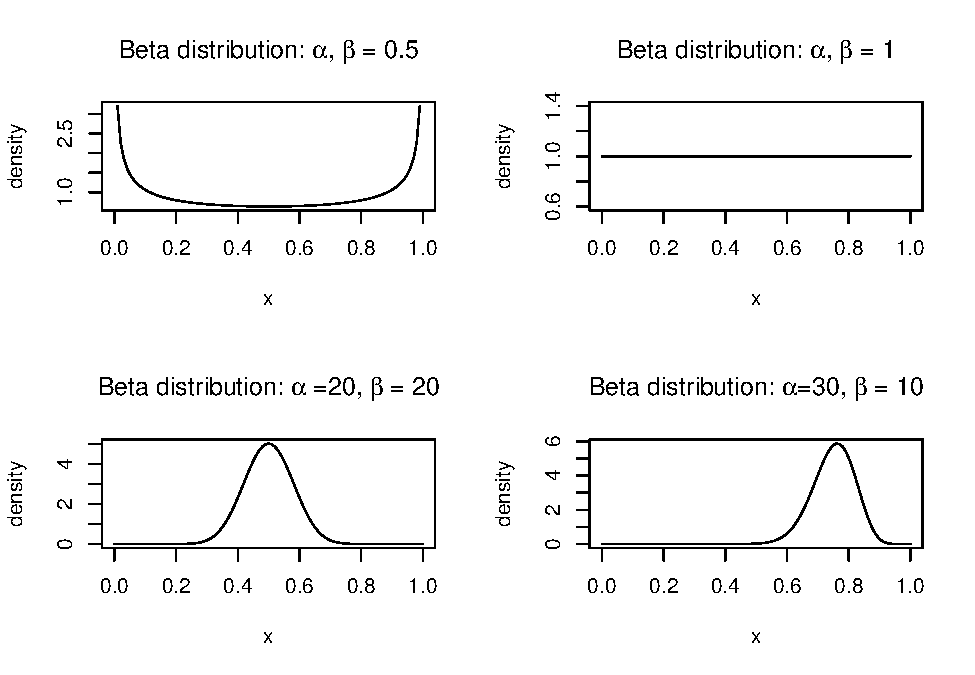
\includegraphics{ii_files/figure-latex/Betas-1.pdf}
\caption{\label{fig:Betas}Beta distributions}
\end{figure}

Dirichlet distributions generalize the Beta to the situation in which there are beliefs not just over a proportion, or a probability, but over collections of probabilities. For example if four outcomes are possible and each is likely to occur with probability \(\theta_k\), \(k=1,2,3,4\) then beliefs about these probabilities are distributions over the a three dimensional unit simplex---that is, all 4 element vectors of probabilities that add up to 1. The distribution has as many parameters as there are outcomes and these are traditionally recorded in a vector, \(\alpha\). Similar to the Beta distribution, an uninformative prior (Jeffrey's prior) has \(\alpha\) parameters of \((.5,.5,.5, \dots)\) and a uniform (``flat'') distribution has \(\alpha = (1,1,1,,\dots)\).

As with the Beta distribution, the Dirichlet updates in a simple way. If you have a Dirichlet prior with parameter \(\alpha = (\alpha_1, \alpha_2, \dots)\) and you observe outcome \(1\), for example, then then posterior distribution is also Dirichlet with parameter vector \(\alpha' = (\alpha_1+1, \alpha_2,\dots)\).

\hypertarget{moments}{%
\subsubsection{Moments}\label{moments}}

In what follows we often refer to the ``posterior mean'' or the ``posterior variance.'' These are simply summary statistics of the posterior distribution and can be calculated easily once the posterior is known. For example the posterior mean of a parameter \(\theta_1\)---just one in a collection of parameters stored in \(\theta\)---is simply \(\overline{\theta}_1 | \mathcal{D} = \int \theta_1 p(\theta | \mathcal{D}) d\theta\). Note importantly that this is calculated using the posterior over the entire vector \(\theta\), there is no notion of updating parameter \(\theta_1\) on its own. Similarly the posterior variance is \(\int (\theta_1 - (\overline{\theta}_1 | \mathcal{D})^2 p(\theta | \mathcal{D}) d\theta\).

\hypertarget{bayes-estimation-in-practice}{%
\subsubsection{Bayes estimation in practice}\label{bayes-estimation-in-practice}}

Although the principle of Bayesian inference is quite simple, in practice calculating posteriors for continuous parameters is computationally complex.

In principle with continuous parameters there is an infinity of possible parameter values. Analytic solutions are not, in general, easy to come by and so in practice researchers use some form of sampling.

Imagine for instance you were interested in forming a posterior on the share intending to vote democrat, given polling data. (This is not truly continuous, but with large elections it might as well be).

One approach is to coarsen the parameter space---we calculate the probability of observing the polling data given possible values \(\theta = 0, \theta = .1, \theta = .2, \dots, \theta = 1\), and, apply Bayes rule to form a posterior for each of these these possibilities. The downside of the this approach is that it for a decent level of precision it becomes computationally expensive with large parameter spaces and parameter spaces get large quickly. For instance if you are interested in vote shares you might find .4, .5, and .6 too coarse and want posteriors for 0.51 or even 0.505; this would require calculations for 200 parameter values. If you had two parameters that you wanted to slice up each into 200 possible values, you would then have 40,000 parameter pairs to worry about. What's more, \emph{most} of those calculations would not be very informative if the real uncertainty all lies in some small (though possibly unknown) range -- such as between 40\% and 60\%.

An alternative approach is to use variants of Markov Chain Monte Carlo sampling. Under these approaches parameter vectors are sampled and their likelihood is evaluated. If they have high likelihood then new parameter vectors near them are draw with a high probability. Based on the likelihood associated with these new draws, new draws are made. The result is a chain of draws that build up to approximate the posterior distribution. The output from these procedures is not a set of probabilities for each possible parameter vector but rather a a set of draws of parameter vectors from the posterior distribution.

Many algorithms have been developed to achieve these tasks efficiently; in all of our applications we rely on the \texttt{stan} procedures which involve\ldots{}.

\hypertarget{bayes-applied}{%
\section{Bayes applied}\label{bayes-applied}}

\hypertarget{bayesian-inference-on-queries}{%
\subsection{Bayesian Inference on Queries}\label{bayesian-inference-on-queries}}

In Chapter 2 we described estimands of interest as queries over the values of root nodes in directed acyclic graphs.

Once queries are defined in terms of the values of roots then formation of beliefs, given data \(W\), about estimands follows immediately from application of Bayes rule.

Let \(Q(u)\) define the value of the query in context \(u\), the updated beliefs about the query are given by the distribution:

\[P(q | W) = \int_{u:Q(u) = q} P(u|W)du =  \int_{u:Q(u) = q} \frac{P(W|u)P(u)}{\int_{u'}P(W|u')P(u')du'}du\]

This expression gathers together all the contexts that produce a given value of \(Q\) and assesses how likely these are, collectively, given the data.\footnote{Learning about roots from observed data is sometimes termed \emph{abduction}; see \citet{pearl2009causality}, p 206.} For an abstract representation of the relations between assumptions, queries, data, and conclusions, see Figure 1 in \citet{pearl2012causal}.

Return now to Mr Smith's puzzle. The two ``roots'' are the sexes of the two children. The query here is \(Q\): ``Are both boys?'' which can be written in terms of the roots. The statement ``\(Q=1\)'' is equivalent to the statement (\(A\) is a boy \& \(B\) is a boy). Thus it takes the value \(q=1\) in just one context. Statement \(q=0\) is the statement (``\(A\) is a boy \& \(B\) is a girl'' or ``\(A\) is a girl \& \(B\) is a boy'' or ``\(A\) is a girl \& \(B\) is a girl''). Thus \(q=0\) in three contexts. If we assume that each of the two children is equally likely to be a boy or a girl with independent probabilities, then each of the four contexts is equally likely.
The result can then be figured out as \(P(Q=1) = \frac{1\times \frac{1}{4}}{1\times \frac{1}{4} + 1\times \frac{1}{4}+1\times \frac{1}{4}+0\times \frac{1}{4}} = \frac{1}{3}\). This answer requires summing over only one context. \(P(Q=0)\) is of course the complement of this, but using the Bayes formula one can see that it can be found by summing over the posterior probability of three contexts in which the statement \(Q=0\) is true.

\hypertarget{bayesian-correlational-inference}{%
\subsection{Bayesian correlational inference}\label{bayesian-correlational-inference}}

In all the examples describe above Bayes rule was used to update inferences about a particular case given additional information about that case. But the same logic works just as well for problems in which one tries to update about a general relation given a set of cases.
The correlational solution to the fundamental problem of causal inference is to focus on \emph{population-level} effects. Rather than seeking to identify the types of particular cases, researchers exploit covariation across cases between the treatment and the outcome variables---i.e., dataset observations---in order to assess the \{average effect\} of treatment on outcomes for a \{population\} or \{sample\} of cases. In the simplest, frequentist approach, under conditions described by \citep{Rubin1974} the average effect of a treatment may be estimated as the difference between the average outcome for those cases that received treatment and the average outcome for those cases that did not receive treatment.

Although this frequentist approach to estimating causal effects from correlational data is more familiar, the problem can also be described in Bayesian terms.\footnote{For a fuller treatment, see for example \citet{heckman2014treatment}.}

\begin{figure}

{\centering 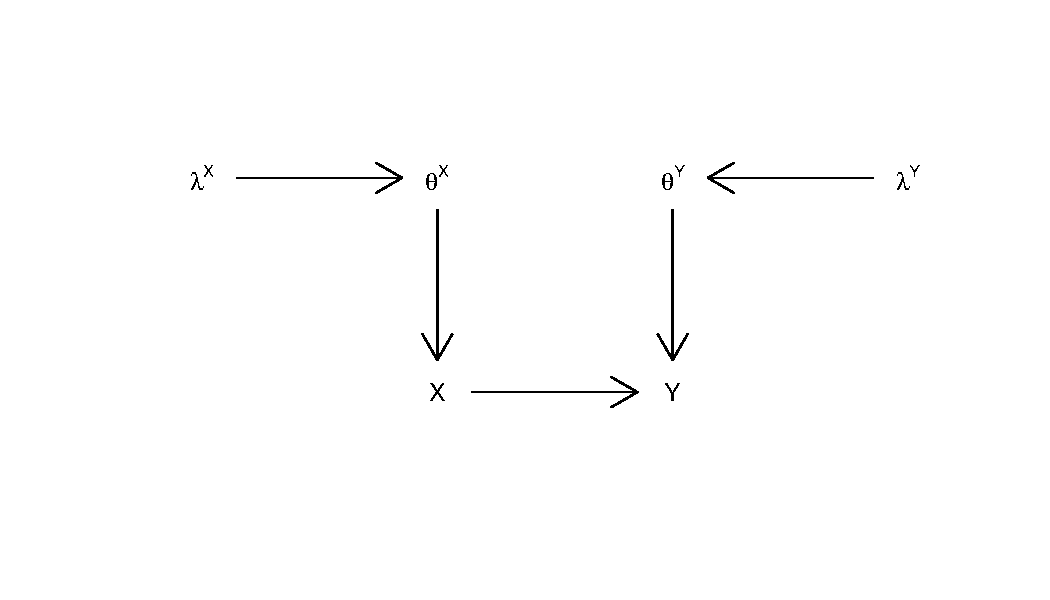
\includegraphics[width=.5\textwidth]{ii_files/figure-latex/simpleXYDAG-1} 

}

\caption{A graph depicting a situation in which it is possible that $X$ causes $Y$; the unit level causal type is $\theta^Y$ and the distribution of causal types is $\lambda^Y$.}\label{fig:simpleXYDAG}
\end{figure}

Suppose we are interested in determining the \emph{distribution} of causal types in a population. We again need to specify our parameters, priors, likelihood, the probability of the data, and the inference strategy.

In turn we have:

\textbf{Parameters.} Our hypothesis consists of a set of \(\lambda\) values: i.e., the proportion of the population of authoritarian regimes for which economic crisis would generate or has generated collapse (\(\lambda_b\)); the proportion for which collapse is inevitable (\(\lambda_d\)); and so on.

We can now define our hypothesis as a vector, \(\lambda = (\lambda^X_0,\lambda^X_1,\lambda^Y_{00},\lambda^Y_{10},\lambda^Y_{01}, \lambda^Y_{11})\), that registers a possible set of values for the parameters over which we will update: type proportions in the population and assignment propensities by type.

\textbf{Prior.} We next need to assign a prior probability to \(\lambda\). In the general case, we will do so by defining a prior probability distribution, \(p(\lambda^j)\), over possible values of the elements of \(\lambda^j\). Here \(\lambda^Y\) has four possible values and we use a Dirichlet distribution on a 3-simplex. \(\lambda^X\) has has only two possible values and in this case the Dirichlet distribution reduces to a Beta distribution.

\textbf{Likelihood.} Our data, \(\mathcal{D}\), consist of \(X\) and \(Y\) observations for a sample of cases. With binary \(X\) and \(Y\), there are four possible data realizations (combinations of \(X\) and \(Y\) values) for a given case. For a single case, it is straightforward to calculate an event probability \(w_{xy}\) \textbar{} that is, the likelihood of observing the particular combination of \(X\) and \(Y\) given the type shares and assignment probabilities in \(\theta\). For instance:

\[w_{00}=\Pr(X=0, Y=0|\theta)=\lambda^X_0(\lambda^Y_{00} + \lambda^Y_{01})\]

More generally, let \(w_{XY}\) denote the vector of these event probabilities for each combination of \(X\) and \(Y\) values, conditional on \(\lambda\). Further, let \(n_{XY}\) denote vector containing the number of cases observed with each \(X,Y\) combination. Under an assumption of independence (data are independently and identically distributed), the full likelihood is then given by the multinomial distribution:
\[\Pr(\mathcal{D}|\lambda)= \text{Multinomial}(n_{XY}  | w_{XY})\]

Note again that here we have assumed that data is randomly drawn. More general functions can allow for more complex data gathering processes.

\textbf{Probability of the data.} We calculate the unconditional probability of the data, \(Pr(\mathcal{D})\), by integrating the likelihood function above over all parameter values, weighted by their prior probabilities.

\textbf{Inference.} After observing our data, \(\mathcal{D}\), we then form posterior beliefs over \(\lambda\) by direct application of Bayes' rule, above:

\[p(\lambda|\mathcal{D}) = \frac{\Pr(\mathcal{D}|\lambda)p(\lambda)}{\int\Pr(\mathcal{D}|\lambda')p(\lambda')d\lambda'}\]

This posterior distribution reflects our updated beliefs about which sets of parameter values are most likely, given the data. Critically, note that, upon observing \(X\) and \(Y\) data, we simultaneously update beliefs about all parameters in \(\lambda\): both beliefs about causal effects (type shares) in the population \emph{and} beliefs about the assignment propensities for \(X\).

We illustrate Bayesian correlational inference with a simple case. Suppose we observe for all postwar authoritarian regimes, whether they did or did not suffer economic crisis and did or did not collapse. Say for simplicity we know that all authoritarian regimes were ``assigned'' to economic crisis with a 0.5 probability during the period under analysis (thus assignment is known to be \emph{as if} random). And assume that, prior to observing \(X\), \(Y\) data we believe that each of two propositions are true with 0.5 probability. Under proposition \textbf{(\(\theta_1\))} all regimes are of type \(b\) (and so the average treatment effect is 1); under proposition \textbf{(\(\theta_2\))} 50\% of regimes are of type \(c\) and 50\% are of type \(d\) (and so the average treatment effect is 0).\footnote{In this simple case we can think of \(\theta\) as being constrained to take on only one of two possible values: \(\theta \in \{\theta_1=\{a=0,b=1, c=0, d=0, \pi_a=0.5,\pi_b=0.5,\pi_c=0.5,\pi_d=0.5\},\{\theta_2=\{a=0,b=0, c=.5, d=.5, \pi_a=0.5,\pi_b=0.5,\pi_c=0.5,\pi_d=0.5\} \}\).}

Applying Bayes' rule, our posterior probability on proposition \(\theta_1\), having observed the data, is:

\begin{eqnarray*}
\Pr(\theta_1|\mathcal{D}) 
=\frac{\Pr(\mathcal{D}|\theta_1)\Pr(\theta_1)}{\Pr(\mathcal{D}|\theta_1)\Pr(\theta_1)+\Pr(\mathcal{D}|\theta_2)\Pr(\theta_2)}
\end{eqnarray*}

or equivalently:

\begin{eqnarray*}
\Pr(b=1|\mathcal{D}) 
%=\frac{\Pr(\mathcal{D}|b=1) \Pr(b=1)}{\Pr(\mathcal{D})}
=\frac{\Pr(\mathcal{D}|\lambda_b=1)\Pr(\lambda_b=1)}{\Pr(\mathcal{D}|\lambda_b=1)\Pr(\lambda_b=1)+\Pr(\mathcal{D}|\lambda_b=0)\Pr(\lambda_b=0)}
\end{eqnarray*}

The event probabilities of each of the observed events is \(0.5\) under \(\theta_1\) but just \(0.25\) under \(\theta_2\). Using the binomial distribution (a special case of the multinomial for this simple case) we know that the chances of such data arising are 1 in 2 under \(\theta_1\) but only 1 in 8 under \(\theta_2\). Our posterior would then be:

\begin{eqnarray*}
\Pr(\lambda_b=1|\mathcal{D}) =\frac{\frac{1}{2} \times \frac{1}{2}}{\frac{1}{2} \times \frac{1}{2} + \frac{1}{8}\times \frac{1}{2}} = \frac{4}{5} 
\end{eqnarray*}

The key difference between this example and more general applications is simply that in the general case we allow for uncertainty --- and updating --- not simply over whether \(\lambda_b\) is 0 or 1, but over a range of possible values for multiple parameters of interest. Though this adds complexity, it does not change the fundamental logic of updating.

\hypertarget{simple-bayesian-process-tracing}{%
\subsection{Simple Bayesian Process Tracing}\label{simple-bayesian-process-tracing}}

Process tracing in its most basic form seeks to use within case evidence to draw inferences about the case. For example, with a focus on whether \(X\) caused \(Y\) , data on a ``clue'', \(K\), is used to make inference about whether or not the outcome in that case was generated by the case's treatment status. We refer to the within-case evidence gathered during process tracing as \emph{clues} in order to underline their probabilistic relationship to the causal relationship of interest. Readers familiar with the framework in \citet{collier2004sources} can usefully think of our ``clues'' as akin to causal process observations, although we highlight that there is no requirement that the clues be generated by the causal process.

To make inferences, the analyst looks for clues that will be observed with some probability if the case is of a given type and that will \emph{not} be observed with some probability if the case is \emph{not} of that type.

It is relatively straightforward to express the logic of process tracing in Bayesian terms, a step that will aid the integration of qualitative with quantitative causal inferences. As noted by others (e.g.~\citet{BennettBayes}, \citet{beachpedersen2013process}, \citet{rohlfing2012case}), there is an evident connection between the use of evidence in process tracing and Bayesian inference. .

In a Bayesian setting, we begin with a prior belief about the probability that a hypothesis is true. New data then allow us to form a posterior belief about the probability of the hypothesis.

Formally, we express Bayes' rule as:
\begin{eqnarray}
\Pr(H|\mathcal{D})=\frac{\Pr(\mathcal{D}|H)\Pr(H)}{\Pr(\mathcal{D})}
\end{eqnarray}

\(H\) represents our hypothesis, which may consist of beliefs about one or more parameters of interest. \(\mathcal{D}\) represents a particular realization of new data (e.g., a particular piece of evidence that we might observe). Thus, our posterior belief derives from three considerations. First, the `'likelihood'': how likely are we to have observed these data if the hypothesis were true, \(\Pr(\mathcal{D}|H\))? Second, how likely were we to have observed these data regardless of whether the hypothesis is true or false, \(\Pr(\mathcal{D})\)? \%These first two questions, then, capture how \{consistent\} the data are with our hypothesis and how \{specific\} the data are to our hypothesis.
Our posterior belief is further conditioned by the strength of our prior level of confidence in the hypothesis, \(\Pr(H)\). The greater the prior likelihood that our hypothesis is true, the greater the chance that new data consistent with the hypothesis has \emph{in fact} been generated by a state of the world implied by the hypothesis.

In formalizing Bayesian process tracing, we start with a very simple Bayesian setup, which we then elaborate. Suppose that we already have \(X,Y\) data on one authoritarian regime: we know that it suffered economic crisis (\(X=1\)) and collapsed (\(Y=1\)). But what caused the collapse? We answer the question by (a.) defining our parameters, which are the key quantities of interest, (b.) stating prior beliefs about the parameters of interest, (c.) defining a likelihood function, (d.) assessing the probability of the data, and (e.) drawing inferences. We discuss each of these in turn.

\textbf{Parameters.} The inferential challenge is to determine whether the regime collapsed \emph{because} of the crisis (\(b\) type) or whether it would have collapsed even without it (\(d\) type). We do so using further information from the case---one or more clues. We use the variable \(K\) to register the outcome of the search for a clue (or collection of clues), with \(K\)=1 indicating that a specific clue (or collection of clues) is searched for and found, and \(K\)=0 indicating that the clue is searched for and not found.

Let \(j\in \{a,b,c,d\}\) refer to the type of an individual case. Our hypothesis, in this initial setup, consists simply of a belief about \(j\) for the case under examination: specifically whether the case is a \(b\) type (\(j=b)\). The parameter of interest is the causal type.\footnote{More formally, we can let our hypothesis be a vector \(\theta\) that contains a set of indicators for the causal type of the case \(\gamma=(\gamma_b, \gamma_d)\), where \(\gamma_j\in\{0,1\}\) and \(\sum \gamma_j = 1\).}

\%While the correlational approach observes multiple regimes to determine whether crisis has an effect `'on average,'' the process tracing approach looks for evidence of a \emph{clue}, \(K\), within the individual case. As described above, t

\textbf{Prior.} We then assign a prior degree of confidence to the hypothesis (\(Pr(H)\)). This is, here, our prior belief that an authoritarian regime that has experienced economic crisis is a \(b\). For now, we express this belief as a prior point probability.

\%Our posterior beliefs then constitute a probability distribution over both the type of the case and \(\phi\) values---representing updating over both the causal effect and our empirical assumptions about clue likelihoods.

\textbf{Likelihood.} We next indicate the likelihood, \(Pr(K=1|H)\). This is the probability of observing the clue, when we look for it in our case, if the hypothesis is true---i.e., here, if the case is a \(b\) type. We thus require beliefs relating clues to causal types.

The key feature of a clue is that the probability of observing the clue is believed by the researcher to be a function of the case's causal type. \%The \emph{differential} probabilities of observing a clue, of \(K=1\), under different types are what allow us to draw inferences from clues to types. We thus need beliefs about the probability of observing the clue, when we look for it, for a case of each type.
For the present example, we will need two such probabilities: we let \(\phi_b\) denote the probability of observing the clue for a case of \(b\) type (\(\Pr(K=1|j=b)\)), and \(\phi_d\) the probability of observing the clue for a case of \(d\) type (\(\Pr(K=1|j=d)\)).\footnote{More fundamentally one might think of types being defined over \(Y\) and \(K\) as a function of \(X\). Thus potential clue outcomes could also be denoted \(K(1)\) and \(K(0)\). High expectations for observing a clue for a \(b\) type then correspond to a belief that many exchangeable units for which \(Y(X)=X\) also have \(K(1)=1\) (whether or not \(K(0)=0\)).} The key idea in process tracing is that the \emph{differences} between these probabilities provides clues with \{`'probative value,''\} that is, the ability to generate learning about causal types.\footnote{\label{fnPV}More formally, we operationalize the concept of probative value in this paper as twice the expected change in beliefs (in absolute value) from searching for a clue that is supportive of a proposition, given a prior of \(0.5\) for the proposition. For example, in determining whether \(j=b\) or \(j=d\) for a given case, starting from a prior of \(0.5\) and assuming \(\phi_b > \phi_d\), the expected learning can be expressed as \(EL = .5(.5\phi_b/(.5\phi_b + .5\phi_d) -.5) +.5 (.5 - (1-\phi_b).5/((1-\phi_b).5 + (1-\phi_d).5))\). The probative value, after simplifying, is then: \(PV = \phi_b/(\phi_b + \phi_d) -(1-\phi_b)/((1-\phi_b) + (1-\phi_d))\), which takes on values between 0 and 1.}

In process tracing, analysts' beliefs about the probabilities of observing clues for cases with different causal effects typically derive from theories of, or evidence about, the causal process connecting \(X\) and \(Y\). Suppose we theorize that the mechanism through which economic crisis generates collapse runs via diminished regime capacity to reward its supporters during an economic downturn. A possible clue to the operation of a causal effect, then, might be the observation of diminishing rents flowing to regime supporters shortly after the crisis. If we believe the theory, then this is a clue that we might believe to be highly probable for cases of type \(b\) that have experienced economic crisis (where the crisis in fact caused the collapse) but of low probability for cases of type \(d\) that have experienced crisis (where the collapse occurred for other reasons). This would imply a high value for \(\phi_b\) and low value for \(\phi_d\).

Here the likelihood, \(\Pr(K=1|H)\), is simply \(\phi_b\).

Note that the likelihood takes account of known features of the data-gathering process. The likelihood given here is based on the implicit assumption that the case is randomly sampled from a population of \(X=Y=1\) cases for which share \(\phi_b\) of the \(b\) cases have clue \(K=1\) and share \(\phi_d\) of the \(d\) cases have clue \(K=1\).

\textbf{Probability of the data.} This is the probability of observing the clue when we look for it in a case, \emph{regardless} of its type, \((\Pr(K=1))\). More specifically, it is the probability of the clue in a treated case with a positive outcome. As such a case can only be a \(b\) or a \(d\) type, this probability can be calculated simply from \(\phi_b\) and \(\phi_d\), together with our beliefs about how likely an \(X=1, Y=1\) case is to be a \(b\) or a \(d\) type.
This probability aligns (inversely) with Van Evera's concept of `'uniqueness.''

\textbf{Inference.} We can now apply Bayes' rule to describe the learning that results from process tracing. If we observe the clue when we look for it in the case, then our \emph{posterior} belief in the hypothesis that the case is of type \emph{b} is:

\begin{eqnarray*}
%\Pr(j = b |X=Y=K=1)&=& \frac{\Pr(K=1|j = b, X=1) \Pr(j = b| X=1, Y=1) }{\Pr(K=1| X=1, Y=1)}
\Pr(j = b |K=1)= \frac{\Pr(K=1|j = b) \Pr(j = b) }{\Pr(K=1)}= \frac{\phi_b \Pr(j = b) }{\phi_b \Pr(j = b)+\phi_d \Pr(j = d)}
\end{eqnarray*}

Suppose, in our running example, that we believe the probability of observing the clue for a treated \(b\) case is \(\phi_b=0.9\) and for a treated \(d\) case is \(\phi_d=0.5\), and that we have prior confidence of \(0.5\) that an \(X=1, Y=1\) case is a \(b\). We then get:

\begin{eqnarray*}
\Pr(j = b |X=Y=K=1)&=&\frac{0.9\times 0.5}{0.9 \times 0.5 + 0.6 \times 0.5}=0.6
\end{eqnarray*}

Analogous reasoning follows for process tracing in cases with other \(X,Y\) values. For an \(X=0, Y=1\) case, for instance, we need beliefs about whether the case is an \(a\) or a \(d\) type and, for the clue being searched for, the values \(\phi_a\) and \(\phi_d\).

As should be clear from the above, the inferential leverage in process tracing comes from differences in the probability of observing \(K=1\) for different causal types. Thus, the logic described here generalizes Van Evera's familiar typology of tests by conceiving of the certainty and uniqueness of clues as lying along a continuum.

Van Evera's four tests (``smoking gun,'' ``hoop,'' ``straw in the wind,'' and ``doubly decisive'') represent, in this sense, special cases---particular regions that lie on the boundaries of a ``probative-value space.'' To illustrate the idea, we represent the range of combinations of possible probabilities for \(\phi_b\) and \(\phi_d\) as a square in Figure \ref{CluesInferences1} and mark the spaces inhabited by Van Evera's tests. As can be seen, the type of test involved depends on both the relative \emph{and} absolute magnitudes of \(\phi_b\) and \(\phi_d\). The probative value of a test depends on the difference between them. Thus, a clue acts as a smoking gun for proposition ``\(b\)'' (the proposition that the case is a \(b\) type) if it is highly unlikely to be observed if proposition \(b\) is false, and more likely to be observed if the proposition is true (bottom left, above diagonal). A clue acts as a ``hoop'' test if it is highly likely to be found if \(b\) is true, even if it still quite likely to be found if it is false. Doubly decisive tests arise when a clue is very likely if \(b\) and very unlikely if not. It is, however, also easy to imagine clues with probative qualities lying in the large space amidst these extremes.

\begin{figure}
\centering
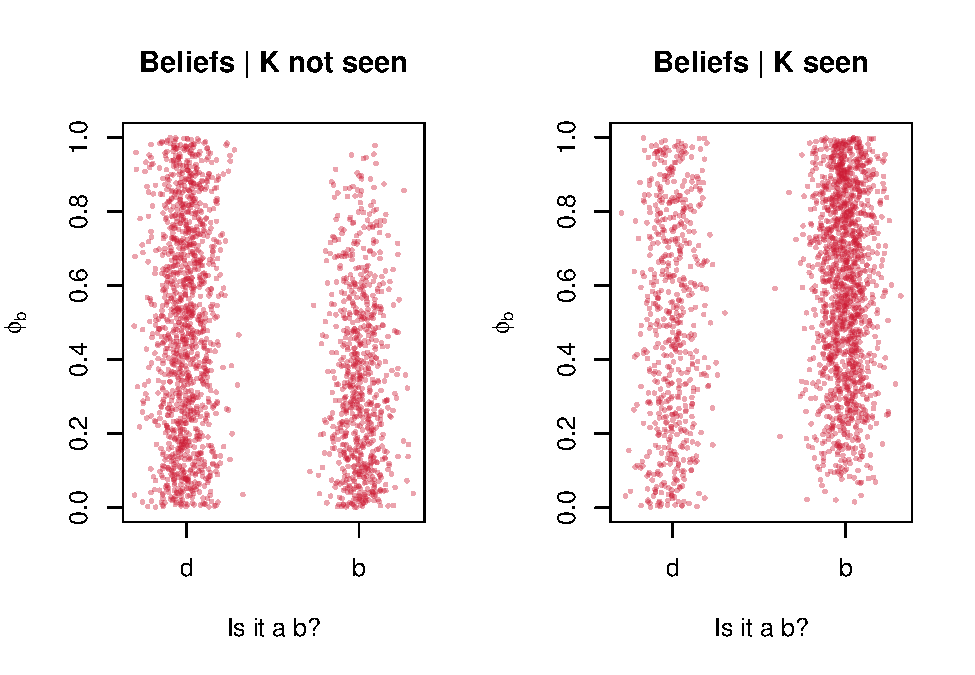
\includegraphics{ii_files/figure-latex/unnamed-chunk-23-1.pdf}
\caption{\label{fig:unnamed-chunk-23}\label{CluesInferences1} A mapping from the probability of observing a clue if the proposition that a case is a \(b\) type is true (\(\phi_b\)) or false (\(\phi_d\)) to a generalization of the tests described in Van-Evera (1997).}
\end{figure}

At the same time, the probative value of a test does not fully describe the learning that takes place upon observing evidence. Following Bayes' rule, inferences also depend on our \emph{prior confidence} in the hypothesis being tested. At very high or very low levels of prior confidence in a hypothesis, for instance, even highly probative evidence has minimal effect on posteriors; the greatest updating generally occurs when we start with moderate prior probabilities. Figure \ref{CluesInferences2} in the Supplementary Materials (\S\ref{AppPriors}) more fully illustrates the effect of prior confidence on learning.

We have so far described a very simple application of Bayesian logic. A further conceptually simple elaboration, however, can place process tracing in a more fully Bayesian setting, allowing for considerable gains in learning. Instead of treating clue probabilities (\(\phi\) values) as fixed, we can treat them as parameters to be estimated from the data. In doing so, we allow the search for clues to provide leverage not only on a case's type but also, given a belief about type, on the likelihood that a case of this type generates the clue. In practice, we define our hypothesis as a vector, \(\theta\), that includes both the causal type of the case and the relevant \(\phi\) values, e.g., \(\phi_b, \phi_d\). We can then define our prior as a prior \emph{probability distribution} \(p(\theta)\) over \(\theta\).\footnote{Here, this distribution could, for example, be given by the product of a categorical distribution over \(\gamma\) (indicators of causal type) and a Beta distribution for each \(\phi_j\).} We can thus express any prior \{uncertainty\} about the relationship between causal effects and clues. Our likelihood is then a function that maps each possible combination of type and the relevant \(\phi\) values to a probability of observing the clue when we search for it.

Updating then produces a joint posterior distribution over type \{and\} our \(\phi\) values. Observing the clue will shift our posterior in favor of type and \(\phi\)-value \{\emph{combinations}\} that are more likely to produce the clue. In sum, and critical to what follows, we can simultaneously update beliefs about \{both\} the case's type \{and\} the probabilities linking types to clues\textbar{}learning both about causal effects and empirical assumptions. We provide further intuition on, and an illustration of, this elaboration in the Supplementary Materials (\ref{AppPriors}).

\hypertarget{three-principles-of-bayesian-updating}{%
\section{Three principles of Bayesian updating}\label{three-principles-of-bayesian-updating}}

\hypertarget{AppPriors}{%
\subsection{Priors matter}\label{AppPriors}}

The amount of learning that results from a given piece of new data depends strongly on prior beliefs. We saw this already with the example of interpreting our test results above. Figure \ref{CluesInferences2} illustrates the point for process tracing inferneces.

In each subgraph of Figure \ref{CluesInferences2} , we show how much learning occurs under different scenarios. The horizontal axis indicates the level of prior confidence in the hypothesis and the curve indicates the posterior belief that arises if we do (or do not) observe the clue. As can be seen, the amount of learning that occurs---the shift in beliefs from prior to posterior---depends a good deal on what prior we start out with. For a smoking gun test, the amount of learning is highest for values roughly in the 0.2 to 0.4 range---and then declines as we have more and more prior confidence in our hypothesis. For a hoop test, the amount of learning when the clue is \emph{not} observed is greatest for hypotheses in which we have middling-high confidence (around 0.6 to 0.8), and minimal for hypotheses in which we have a very high or a very low level of confidence.

\begin{figure}
\centering
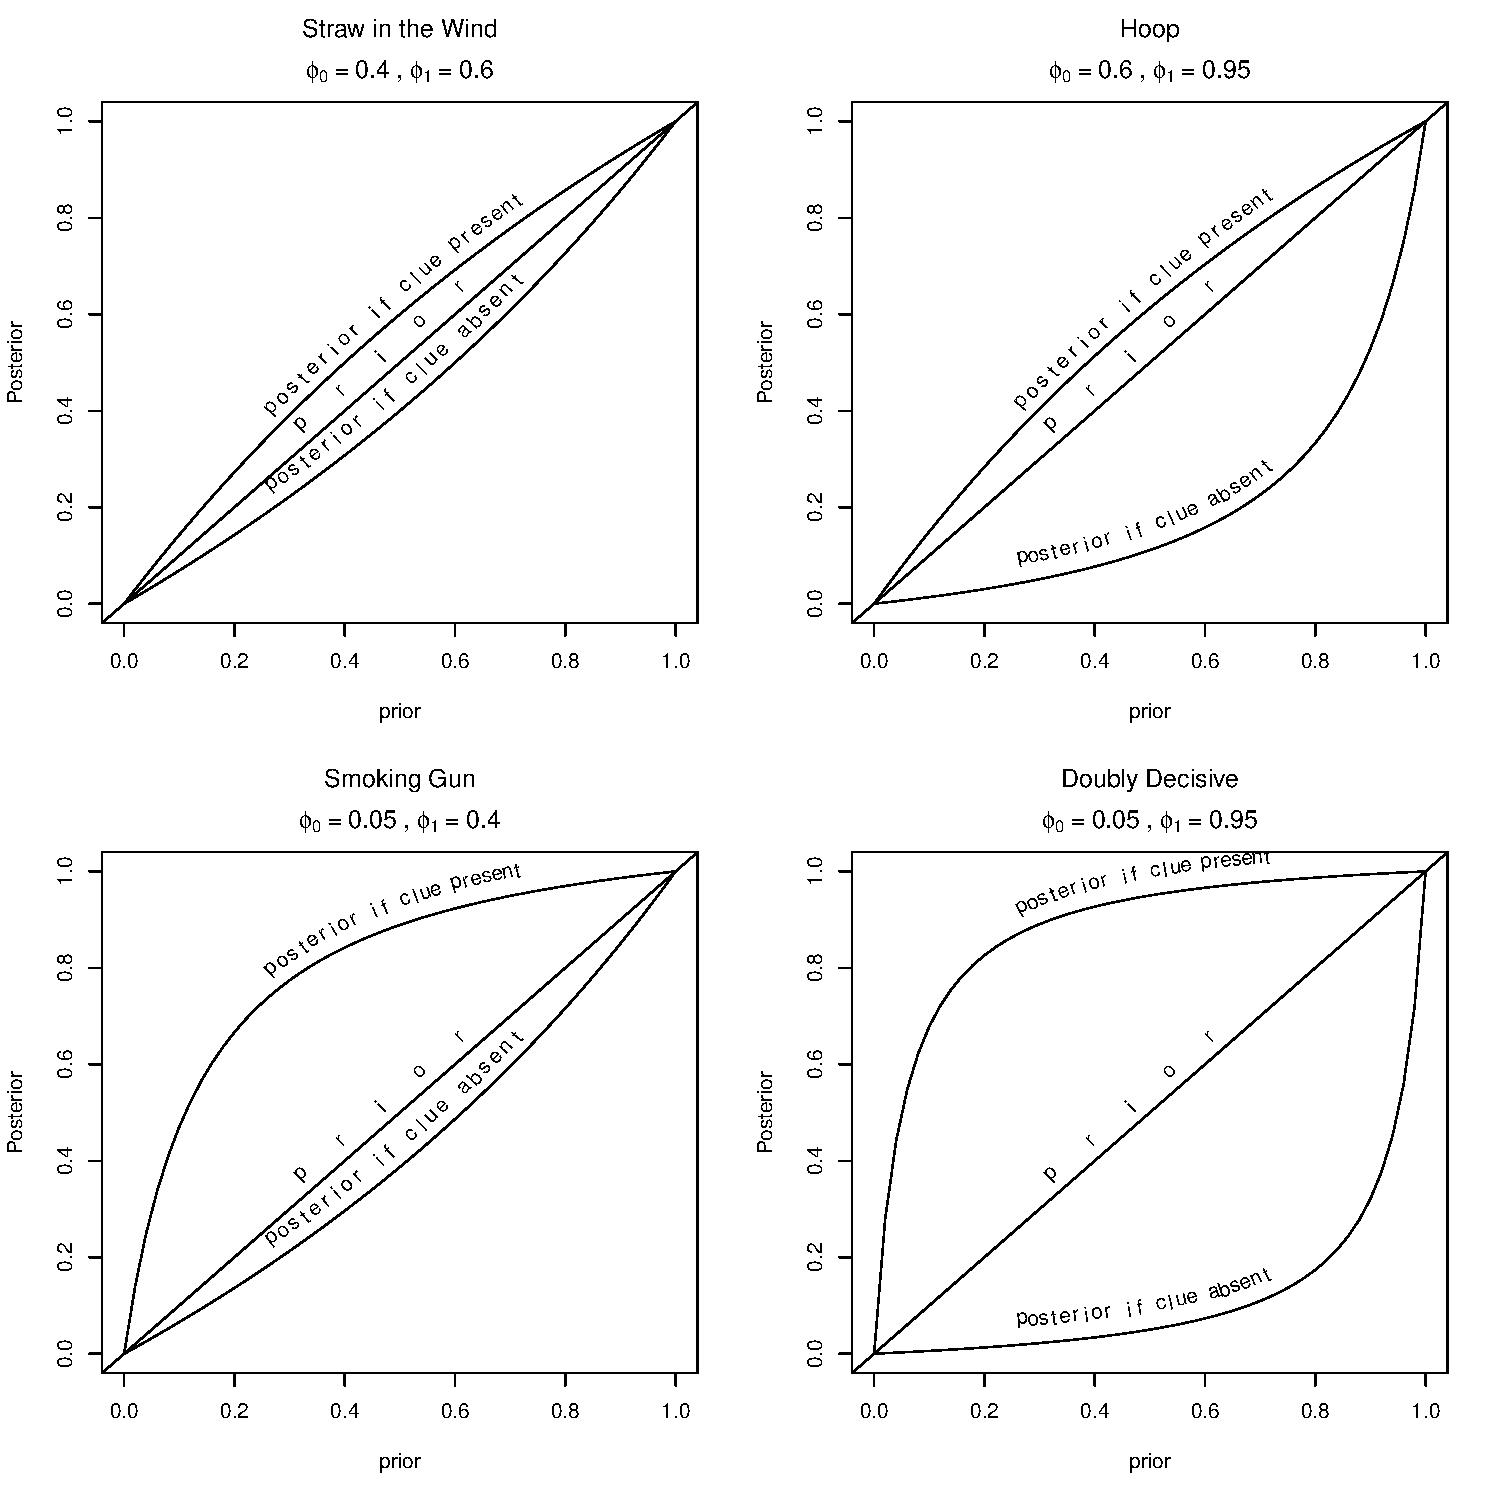
\includegraphics{ii_files/figure-latex/CluesInferences2-1.pdf}
\caption{\label{fig:CluesInferences2}Figure shows how the learning from different types of tests depends on priors regarding the proposition. A smoking gun test has the greatest impact on beliefs when priors are middling low and the clue is observed; a `'hoop test'' has the greatest effect when priors are middling high and the clue is not observed.}
\end{figure}

The implication here is that our inferences with respect to a hypothesis must be based not just on the search for a clue predicted by the hypothesis but also on the \emph{plausibility} of the hypothesis, based on other things we know. Suppose, for instance, that we fail to observe evidence that we are 90 percent sure we \emph{should} observe if a hypothesized causal effect has occurred: a strong hoop test is failed. But suppose that the existing literature has given us a very high level of confidence that the hypothesis \emph{is} right. This high prior confidence, sometimes referred to as a ``base rate,'' is equivalent to believing that the causal effect exists in a very high proportion of cases. Thus, while any given case with a causal effect has only a 0.1 chance of not generating the clue, the high base rate means that the vast majority of cases that we observe without the clue will nonetheless be cases with causal effects. Thus, the failure of even a strong hoop test, involving a highly certain prediction, should only marginally reduce our confidence in a hypothesis that we strongly expect to be true.

A similar line of reasoning applies to smoking gun tests involving hypotheses that prior evidence suggests are very unlikely to be true. Innocent people may be very unlikely to be seen holding smoking guns after a murder. But if a very high proportion of people observed are known to be innocent, then a very high proportion of those holding smoking guns will in fact be innocent---and a smoking-gun clue will be far from decisive.

We emphasize two respects in which these implications depart from common intuitions. First, we cannot make \emph{general} statements about how decisive different categories of test, in Van Evera's framework, will be. It is commonly stated that hoop tests are devastating to a theory when they are failed, while smoking gun tests provide powerful evidence in favor of a hypothesis. But, in fact the amount learned depends not just on features of the clues but also on prior beliefs.

Second, although scholars frequently treat evidence that goes against the grain of the existing literature as especially enlightening, in the Bayesian framework the contribution of such evidence may sometimes be modest, precisely because received wisdom carries weight. Thus, although the discovery of \emph{disconfirming} evidence---an observation thought to be strongly inconsistent with the hypothesis---for a hypothesis commonly believed to be true is more informative (has a larger impact on beliefs) than \emph{confirming} evidence, this does not mean that we learn more than we would have if the prior were weaker. \% But it is not true as a general proposition that we learn more the bigger the ``surprise'' a piece of evidence is.
\%The effect of disconfirming evidence on a hypothesis about which we are highly confident will be \emph{smaller} than it would be for a hypothesis about which we are only somewhat confident.
When it comes to very strong hypotheses, the ``discovery'' of disconfirming evidence is very likely to be a false negative; likewise, the discovery of supporting evidence for a very implausible hypothesis is very likely to be a false positive. The Bayesian approach takes account of these features naturally.\footnote{We note, however, that one common intuition---that little is learned from disconfirming evidence on a low-plausibility hypothesis or from confirming evidence on a high-plausibility one---\emph{is} correct.}

\hypertarget{simultaneoues-joint-updating}{%
\subsection{Simultaneoues, joint updating}\label{simultaneoues-joint-updating}}

When we update we often update over multiple quantities. When we see a smoking gun, for instance, we might update our beliefs that the butler did it, but we might also update our beliefs baout how likely we are to see smoking guns -- maybe they are not so rare as we thought!

Intuitively you might think of this updating as happening sequentially -- first of all you update over the general proposition, then you update over the particular claim. But in fact you update over both quantities at once.

Here we elaborate on the intuition of fully Bayesian process tracing, in which updating occurs over both causal type (\(j\)) and beliefs about the probabilities with which clues are observed for each type (\(\phi\) values). The illustration in the text makes clear how updating over type occurs, given beliefs about \(\phi\) values. But how does updating over \(\phi\) occur?

Suppose that we observe a case with values \(X=1, Y=1\). We begin by defining a prior probability distribution over each parameter. Suppose that we establish a prior categorical distribution reflecting uncertainty over whether the case is a \(b\) type (e.g., setting a probability of 0.5 that it is a \(b\) and 0.5 that is a \(d\) type). We also start with priors on \(\phi_b\) and \(\phi_d\). For concreteness, suppose that we are certain that the clue is unlikely for a \(d\) type (\(\phi_d=.1\)), but we are very uncertain about \(\phi_b\); in particular, we have a uniform prior distribution over \([0,1]\) for \(\phi_b\). Note that, even though we are very uncertain about \(\phi_b\), the clue still has probative value, arising from the fact that the expected value of \(\phi_b\) is higher than that of \(\phi_d\).

Suppose that we then look for the clue in the case and observe it. This observation shifts posterior weight away from a belief that the case is a \(b\). See Figure \ref{fig:correlation} for an illustration. Yet it \emph{simultaneously} shifts weight toward a higher value for \(\phi_b\) and a lower value for \(\phi_d\). The reason is that the observed clue has a relatively high likelihood \emph{both} for combinations of parameter values in which the case is a \(d\) and \(\phi_b\) is low \emph{and} for combinations in which the case is a \(b\) and \(\phi_b\) is \emph{high} (or, equivalently, in this example, where \(\phi_d\) is low). The marginal posterior distribution of \(\phi_b\) will thus be shifted upward relative to its prior marginal distribution. The joint posterior distribution will also reflect a dependency between the probability that the case is a \(b\) vs.~a \(d\), on the one hand, and \(\phi_b\) and \(\phi_d\) on the other.

\begin{figure}
\centering
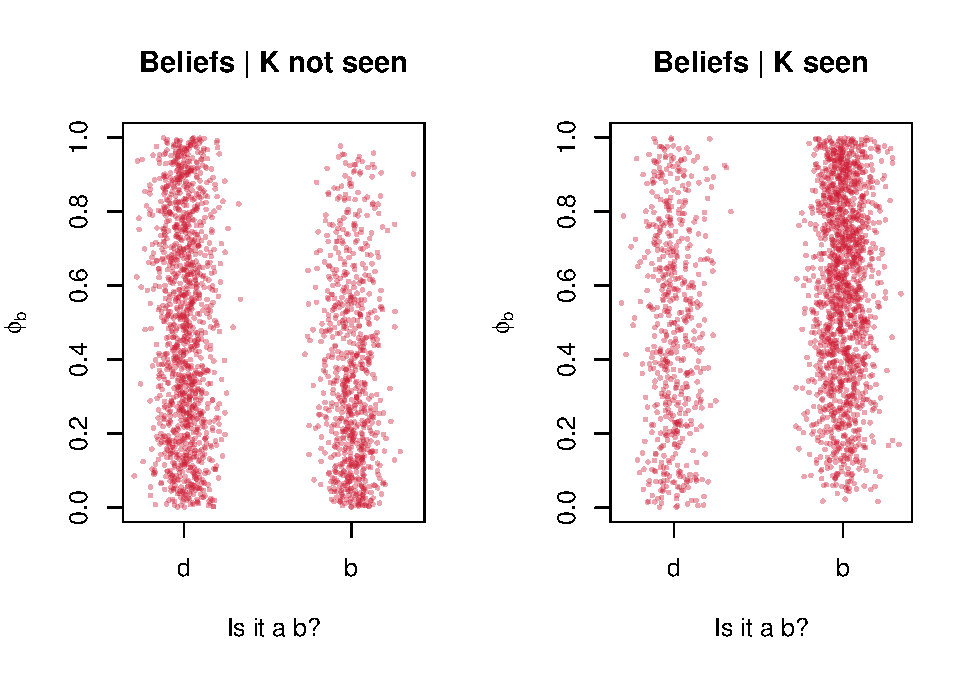
\includegraphics{ii_files/figure-latex/unnamed-chunk-24-1.pdf}
\caption{\label{fig:unnamed-chunk-24}\label{fig:correlation} Joint posteriors distribution on whether a case is a \(b\) or \(d\) and on the probability of seeing a clue for a \(b\) type (\(\phi_b\)).}
\end{figure}

\hypertarget{posteriors-are-independent-of-the-ordering-of-data}{%
\subsection{Posteriors are independent of the ordering of data}\label{posteriors-are-independent-of-the-ordering-of-data}}

We often think of learning as a process in which we start off with some set of beliefs---our priors, we gather data, \(D_1\), and update our beliefs, forming a posterior; we then observe new data and we update again, forming a new posterior, having treated the previous posterior as a new prior. In such cases it might seem natural that it matters which data we saw first and which later.

For instance EXAMPLE

In fact though, Bayesian updating is deaf to ordering. If we learn first that hte card is a face card and second that it is black, our posteriors that it is a Jackk of Spades go from 1 in 52 to 1 in 12 to 1 in 6. If we learn first that the card is black and second that it is a facecard, our posteriors that it is a Jack of Spades go from 1 in 52 to 1 in 26 to 1 in 6. We end up in the same places in both cases. And we would ave had the same conclusion if we learned in one go that the card is a black facecard.

The math of this is easy enough. Our posterior given two sets of data \(D_1, D_2\) can be written:

\[p(\theta | D_1, D_2) = \frac{p(\theta, D_1, D_2)}{p(D_1, D_2)} = \frac{p(\theta, D_1 | D_2)p(D_2)}{p(D_1 | D_2)p(D_2)}= \frac{p(\theta, D_1 | D_2)}{p(D_1 | D_2)}\]

or, equivalently:

\[p(\theta | D_1, D_2) = \frac{p(\theta, D_1, D_2)}{p(D_1, D_2)} = \frac{p(\theta, D_2 | D_1)p(D_1)}{p(D_2 | D_1)p(D_1)}= \frac{p(\theta, D_2 | D_1)}{p(D_2 | D_1)}\]

In other words our posteriors given both \(D_1\) and \(D_2\) can be thought of as the result of updating on \(D_2\) given we already know \(D_1\) or the result of updating on \(D_1\) given we already know \(D_2\).

This fact will be useful in applications. In practice we might assume that we have beliefs based on background data \(D_1\), for example regarding general relations between \(X\) and \(Y\) and a flat prior, and we then update again with new data on \(K\). Rather than updating twice, the fact that updating is invariant to order means that we can assume a flat prior and update once given data on \(X\), \(Y\), and \(K\).

\hypertarget{part-model-based-causal-inference}{%
\part{Model-Based Causal Inference}\label{part-model-based-causal-inference}}

\hypertarget{clues}{%
\chapter{Process Tracing with Causal Models}\label{clues}}

\begin{center}\rule{0.5\linewidth}{\linethickness}\end{center}

We connect the literature on causal models to qualitative inference strategies used in process tracing. We provide a procedure for general inference on case level queries from causal models and walk through applications with simple models. In addition we extract a set of general principles for model based process tracing. We show how a key result from the causal models literature provides a condition for when clues may be (or certainly will not be) informative.

\begin{center}\rule{0.5\linewidth}{\linethickness}\end{center}

We have described the general problem of process tracing as using observable data to make inferences about unobserved, or unobservable parts of a causal structure. We describe a procedure for doing this and then turn to ask whether we can say when, in general, there are data supports updating on estimands of interest.

\hypertarget{process-tracing-and-causal-models}{%
\section{Process tracing and causal models}\label{process-tracing-and-causal-models}}

We focus in this chapter on the particular case of drawing inferences about a single case from a causal model and case level data. The causal model may itself be derived from data from other case (as described in Chapter 8) or it might reflect a theoretical position,

\hypertarget{general-approach}{%
\subsection{General approach}\label{general-approach}}

The general approach to inference draws on the components we outlined in chapters 2 to 4. We focus on the case with binary variables and later describe how this can be extended. Though the examples in this section are for simple models the approach outlined here can be applies to \emph{any} binary causal model and any estimands defined over the model.

\textbf{Model.} We begin with a causal model which describes a set of variables and the parent-child reltions between them---these relationship tell us which (non descendent) variables a given variable is \emph{not} independent of given the other variables in the model.

\textbf{Nodal types}. A node with \(k\) parents has \(2^{\left(2^k\right)}\) ``nodal'' types. For instance if \(Y\) is possibly caused by \(X_1\) and \(X_2\) there are 16 possible causal types for \(Y\), corresponding to the \(2^4\) values that \(Y\) could take given \(X_1\) and \(X_2\) take any of the four values \((0,0), (0,1), (1,0), (1,1)\). We let \(\theta^j\) indicate our beliefs over the noed \(j\) type of a unit at hand.

\textbf{Causal types}. A model in which each node \(j\) has \(k_j\) parents has \(\prod_j2^{\left(2^{k_j}\right)}\) ``causal types'' that uniquely determine what data will be observed for a type under all possible interventions. A causal type is simple a listing that contains one nodal types for each node. For instance \(\theta = (\theta^X = \theta^X_1, \theta^T = \theta^Y_{11})\).

\textbf{Priors}: In the case of no unobserved confounding, our beliefs over a causal type are simply the product of our beliefs over the nodal types. For instance a causal type might be ``a unit in which \(X=1\) and in which \(Y=1\) no matter what value \(X\) takes.'' Let \(\lambda_j\) denote a probability distribution over the values of \(\theta^j\), such that, \(\lambda^Y_{01}\) for instance, is the probability that type \(\theta^Y\) is \(\theta^Y_{01}\). In this case the probability that a unit has a causal type might be written \(\Pr(\theta^X = \theta^X_1)\Pr(\theta^Y = \theta^Y_{11}) = \lambda^X_1\lambda^Y_{11}\).

In the case of unobserved confounding, our beliefs over causal types are still well defined, but they are no longer the simple product of beliefs over nodal types. For instance we might fall back on the general formulation: \(\Pr(\theta^X = \theta^X_1, \theta^Y = \theta^Y_{11}) = \Pr(\theta^X = \theta^X_1)\Pr(\theta^Y = \theta^Y_{11}|\theta^X = \theta^X_1)\). In this case the number of parameters may exceed the number of nodal types, with, for instance parameters \(\hat{\lambda}^Y_{11}\) representing \(\Pr(\theta^Y = \theta^Y_{11}|\theta^X = \theta^X_1)\) and \(\tilde{\lambda}^Y_{11}\) representing \(\Pr(\theta^Y = \theta^Y_{11}|\theta^X = \theta^X_0)\).

\textbf{Possible data patterns.} Each possible causal type maps into a single data pattern. For example, causal type \(\theta = (\theta^X = \theta^X_1, \theta^T = \theta^Y_{11})\) imples data \(X=1, Y=1\). The mapping is not however 1 to 1: in general, multiple causal types can map into the same data type. The mapping can be summarized by an ``ambiguity matrix'' that says which causal types (rows) map into which data types (columns).

Using the \texttt{gbiqq} package we provide two examples of such ambiguity matrices. For an \(X \rightarrow Y\) model:

\begin{table}[t]

\caption{\label{tab:unnamed-chunk-27}Ambiguity matrix for X -> Y model. Rows are causal types, columns are data types. Last column shows possible priors over rows.}
\centering
\begin{tabular}{l|r|r|r|r|r}
\hline
  & X0Y0 & X1Y0 & X0Y1 & X1Y1 & prior\\
\hline
X0Y00 & 1 & 0 & 0 & 0 & 0.1\\
\hline
X1Y00 & 0 & 1 & 0 & 0 & 0.1\\
\hline
X0Y10 & 0 & 0 & 1 & 0 & 0.1\\
\hline
X1Y10 & 0 & 1 & 0 & 0 & 0.1\\
\hline
X0Y01 & 1 & 0 & 0 & 0 & 0.2\\
\hline
X1Y01 & 0 & 0 & 0 & 1 & 0.2\\
\hline
X0Y11 & 0 & 0 & 1 & 0 & 0.1\\
\hline
X1Y11 & 0 & 0 & 0 & 1 & 0.1\\
\hline
\end{tabular}
\end{table}

Here the column names have the obvious interpretation---\(X0Y0\) means a unit with \(X=0, Y=0\) observed. The row names are a concatenation of the nodal types that yield a causal type.\footnote{These nodal types can require many indices--\(2^k\) for a node with \(k\) parents---and the rule we follow is that the \(i\)th subscript indicates the value the node takes when parent \(j \in {1, 2, ..., k}\) take values \(\mod(floor((i-1)/(2^{j-1})), 2)\) For instance for \texttt{Y0111} the first index means that Y takes the value 0 where both parents are 0, in all other cases it takes value 1.}

For an \(X \rightarrow M \rightarrow Y\) model:

\begin{table}[t]

\caption{\label{tab:unnamed-chunk-28}Ambiguity matrix for X -> M -> Y model. Rows are causal types, columns are data types. Last column shows possible priors over rows.}
\centering
\begin{tabular}{l|r|r|r|r|r|r|r|r|r}
\hline
  & X0M0Y0 & X1M0Y0 & X0M1Y0 & X1M1Y0 & X0M0Y1 & X1M0Y1 & X0M1Y1 & X1M1Y1 & prior\\
\hline
X0M00Y00 & 1 & 0 & 0 & 0 & 0 & 0 & 0 & 0 & 0.02\\
\hline
X1M00Y00 & 0 & 1 & 0 & 0 & 0 & 0 & 0 & 0 & 0.02\\
\hline
X0M10Y00 & 0 & 0 & 1 & 0 & 0 & 0 & 0 & 0 & 0.02\\
\hline
X1M10Y00 & 0 & 1 & 0 & 0 & 0 & 0 & 0 & 0 & 0.02\\
\hline
X0M01Y00 & 1 & 0 & 0 & 0 & 0 & 0 & 0 & 0 & 0.04\\
\hline
X1M01Y00 & 0 & 0 & 0 & 1 & 0 & 0 & 0 & 0 & 0.04\\
\hline
X0M11Y00 & 0 & 0 & 1 & 0 & 0 & 0 & 0 & 0 & 0.02\\
\hline
X1M11Y00 & 0 & 0 & 0 & 1 & 0 & 0 & 0 & 0 & 0.02\\
\hline
X0M00Y10 & 0 & 0 & 0 & 0 & 1 & 0 & 0 & 0 & 0.02\\
\hline
X1M00Y10 & 0 & 0 & 0 & 0 & 0 & 1 & 0 & 0 & 0.02\\
\hline
X0M10Y10 & 0 & 0 & 1 & 0 & 0 & 0 & 0 & 0 & 0.02\\
\hline
X1M10Y10 & 0 & 0 & 0 & 0 & 0 & 1 & 0 & 0 & 0.02\\
\hline
X0M01Y10 & 0 & 0 & 0 & 0 & 1 & 0 & 0 & 0 & 0.04\\
\hline
X1M01Y10 & 0 & 0 & 0 & 1 & 0 & 0 & 0 & 0 & 0.04\\
\hline
X0M11Y10 & 0 & 0 & 1 & 0 & 0 & 0 & 0 & 0 & 0.02\\
\hline
X1M11Y10 & 0 & 0 & 0 & 1 & 0 & 0 & 0 & 0 & 0.02\\
\hline
X0M00Y01 & 1 & 0 & 0 & 0 & 0 & 0 & 0 & 0 & 0.04\\
\hline
X1M00Y01 & 0 & 1 & 0 & 0 & 0 & 0 & 0 & 0 & 0.04\\
\hline
X0M10Y01 & 0 & 0 & 0 & 0 & 0 & 0 & 1 & 0 & 0.04\\
\hline
X1M10Y01 & 0 & 1 & 0 & 0 & 0 & 0 & 0 & 0 & 0.04\\
\hline
X0M01Y01 & 1 & 0 & 0 & 0 & 0 & 0 & 0 & 0 & 0.08\\
\hline
X1M01Y01 & 0 & 0 & 0 & 0 & 0 & 0 & 0 & 1 & 0.08\\
\hline
X0M11Y01 & 0 & 0 & 0 & 0 & 0 & 0 & 1 & 0 & 0.04\\
\hline
X1M11Y01 & 0 & 0 & 0 & 0 & 0 & 0 & 0 & 1 & 0.04\\
\hline
X0M00Y11 & 0 & 0 & 0 & 0 & 1 & 0 & 0 & 0 & 0.02\\
\hline
X1M00Y11 & 0 & 0 & 0 & 0 & 0 & 1 & 0 & 0 & 0.02\\
\hline
X0M10Y11 & 0 & 0 & 0 & 0 & 0 & 0 & 1 & 0 & 0.02\\
\hline
X1M10Y11 & 0 & 0 & 0 & 0 & 0 & 1 & 0 & 0 & 0.02\\
\hline
X0M01Y11 & 0 & 0 & 0 & 0 & 1 & 0 & 0 & 0 & 0.04\\
\hline
X1M01Y11 & 0 & 0 & 0 & 0 & 0 & 0 & 0 & 1 & 0.04\\
\hline
X0M11Y11 & 0 & 0 & 0 & 0 & 0 & 0 & 1 & 0 & 0.02\\
\hline
X1M11Y11 & 0 & 0 & 0 & 0 & 0 & 0 & 0 & 1 & 0.02\\
\hline
\end{tabular}
\end{table}

\textbf{Updating on types.} Updating on the distribution of causal types given the \emph{complete} data is then straightforward. Still assuming a single case, when we observe data we place 0 weight on all causal types that could not have produced this data and then scale up weights on all causal types that could have.

In terms of the ambiguity matrices, we start out with a set of probability weights on all rows of the ambiguity matrix. If we observe data corresponding to a given column of the ambiguity matrix, we put 0 weight on all rows that do not contain a 1 in this column and scale up weights on all rows that do contain a 1. For instance in the case with \(X=Y=1\) our updated matrix would be:

\begin{tabular}{r|r|r}
\hline
X1Y1 & prior & posterior\\
\hline
1 & 0.2 & 0.6667\\
\hline
1 & 0.1 & 0.3333\\
\hline
\end{tabular}

In the case with model \(X \rightarrow M \rightarrow Y\) and data \(X=M=Y=1\) this exercise would yield:

\begin{tabular}{l|r|r|r}
\hline
type & X1M1Y1 & prior & posterior\\
\hline
X1M01Y01 & 1 & 0.08 & 0.44\\
\hline
X1M11Y01 & 1 & 0.04 & 0.22\\
\hline
X1M01Y11 & 1 & 0.04 & 0.22\\
\hline
X1M11Y11 & 1 & 0.02 & 0.11\\
\hline
\end{tabular}

The same logic applies if partial data is observed, except now rather than reducing to one column we entertain the possibility of any column consistent with the observed data. For instance if \(M\) is not observed we have:

\begin{tabular}{l|r|r|r|r}
\hline
type & X1M0Y1 & X1M1Y1 & prior & posterior\\
\hline
X1M00Y10 & 1 & 0 & 0.02 & 0.08\\
\hline
X1M10Y10 & 1 & 0 & 0.02 & 0.08\\
\hline
X1M01Y01 & 0 & 1 & 0.08 & 0.31\\
\hline
X1M11Y01 & 0 & 1 & 0.04 & 0.15\\
\hline
X1M00Y11 & 1 & 0 & 0.02 & 0.08\\
\hline
X1M10Y11 & 1 & 0 & 0.02 & 0.08\\
\hline
X1M01Y11 & 0 & 1 & 0.04 & 0.15\\
\hline
X1M11Y11 & 0 & 1 & 0.02 & 0.08\\
\hline
\end{tabular}

\textbf{Updating on estimands.} We now have a posterior over the case level model itself and posteriors over any particular estimand can be expressed as a combination of these. For instance the estimand ``\(X=1\) caused \(Y=1\)'' in the \(X \rightarrow M \rightarrow Y\) model is equivalent to the statement ``The type is either''\(X=1\) and \(X=1\) causes \(M=1\) and \(M=1\) causes \(Y=1\)" or ``\(X=1\) and \(X=1\) causes \(M=0\) and \(M=0\) causes \(Y=1\)''.

Relating causal types to estimands can be tricky when the number of types gets large. In practive we use a function to do this for us. For example the estimand ``\(X\) matters for \(Y\)'' is a relatively large though still easily calculated collection of types:

\begin{Shaded}
\begin{Highlighting}[]
\KeywordTok{get_types}\NormalTok{(XMY, }\StringTok{"Y[X=1] != Y[X=0]"}\NormalTok{)}
\end{Highlighting}
\end{Shaded}

\begin{verbatim}
X0.M10.Y10, X1.M10.Y10, X0.M01.Y10, X1.M01.Y10, X0.M10.Y01, X1.M10.Y01, X0.M01.Y01, X1.M01.Y01
\end{verbatim}

The posterior on the estimand is then just given by summing up the posterior probability on each of the causal types that correspond to the estimand.

That completes the abstract representation of the procedure. We now build up the intuition by walking through the procedure for simple mediation and moderation models.

\hypertarget{walk-through-using-a-simple-mediation-model}{%
\subsection{Walk through using a simple mediation model}\label{walk-through-using-a-simple-mediation-model}}

Suppose that, in a binary setting, we have observed \(X=1\) and \(Y=1\) in a case, but we do not know and want to learn if \(X\) caused \(Y\) here. So, for instance, we see that a country has a free press, and that its government was removed; but we want to find out whether the free press caused government removal. In other words, we want to know the value of \(\theta_Y^{higher}\). Suppose, further, that we have a theory---a lower-level model---of the effect of \(X\) on \(Y\) represented by the graph in Figure \ref{fig:Kinf}. Say, a free press causes government removal through media reports of corruption. What can be learned, then, from observing the moderator, \(K\), given this lower-level model?

\begin{figure}

{\centering 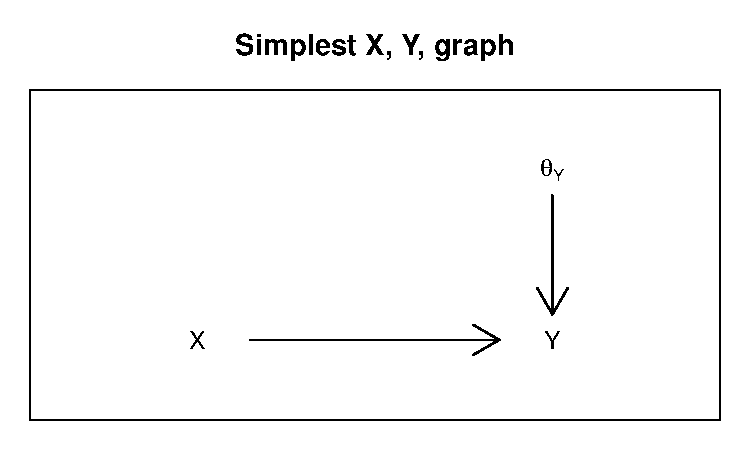
\includegraphics[width=.7\textwidth]{ii_files/figure-latex/unnamed-chunk-34-1} 

}

\caption{\label{fig:Kinf} A model with one explanatory variable and one mediator.}\label{fig:unnamed-chunk-34}
\end{figure}

Observing \(X=1, Y=1\) already tells us that \(\theta_Y^{higher}\), the higher-level type variable for \(X\)'s effect on \(Y\), takes on either \(\theta_{01}\) or \(\theta_{11}\): either \(X\) has had a positive effect on \(Y\) or it has no effect (\(Y\) would be \(1\) regardless of \(X\)'s value). We now want the mediator clue, \(K\), to help us distinguish between these possibilities. What could we learn if we went looking for information on \(K\) and observed \(K=1\)?

When we combine this observation for \(K\) with the observations we already have for \(X\) and for \(Y\), we can begin to eliminate values for the type nodes in the lower-level model. First, seeing \(K=1\) with \(X=1\) eliminates two possible values of \(K\)'s response type, \(\theta_K\): \(\theta_{00}^{K}\) and \(\theta_{10}^{K}\). That is, by observing \(X=1\) and \(K=1\), we know that \(K\) is not fixed at \(0\), and we know that \(X\) does not have a negative effect on \(K\). So, for instance, if we observe a high number of media reports in corruption (along with a free press and government removal), we know (1) that reports of corruption are not fixed at a low level in this case and (2) that a free press does not cause a low level of media reports in this case.

Second, observing \(K=1\) with \(Y=1\) allows us to rule out the values \(\theta_{00}^{Y}\) and \(\theta_{10}^{Y}\) for \(Y\)'s response type node, \(\theta_Y^{lower}\): we have learned that \(Y\) is not ``stuck'' at \(0\), regardless of \(K\)'s value; and we have learned that \(K\) does not exert a negative effect on \(Y\). Observing together many corruption reports and government removal tells us (1) that government removal can occur in this case and (2) that media reports of corruption do not prevent government removal.

So what have we learned? By eliminating these two pairs of lower-level types we have excluded three possible causal sequences that could be consistent with our initial observation of \(X=Y=1\)---that is, with the two higher-level types that are in contention (\(\theta_{01}\), or \(b\)-type, and \(\theta_{11}\)), or \(d\)-type). The first excluded sequence---which would be theoretically consistent with a \(d\) response-type at the higher level---is that \(K\) is fixed at \(0\), followed by \(Y\) being \(1\) for some other reason. Second, we have ruled out the possibility that---also consistent with a higher-level \(d\) type---that \(X\) has a negative effect on \(K\), followed by no effect of \(K\) on \(Y\) because \(Y\) is fixed at \(0\). Third, we have excluded the possibility---consistent with a positive effect of \(X\) on \(Y\)---that \(X\) has a negative effect on \(K\) and that \(K\) in turn has a negative effect on \(Y\).

At this point, however, the learning we have achieved is purely formal, stuck in the realm of lower-level types. While we have eliminated values of lower-level type variables and their associated sequences, doing so does not yet speak to the question of interest: it does not eliminate either of the original two \emph{higher}-level types, \(\theta_{01}\) and \(\theta_{11}\), that could define \(Y\)'s response to \(X\). The observed data (\(X=K=Y=1\)) are consistent with \(X\) having a positive effect on \(Y\) via linked positive effects (\(\theta_K=\theta_{01}^K\) and \(\theta_Y^{lower}=\theta_{01}^Y\)); and they are consistent with \(X\) having no effect on \(Y\), whether because \(K\) is always \(1\) (\(\theta_K=\theta_{11}^K\)), because \(Y\) is always \(1\) (\(\theta_Y^{lower}=\theta_{11}^Y\)), or both. Tracing out a series of events between possible cause and outcome cannot by itself deliver a causal inference. We might observe a free press, corruption reports, and government removal, picking up clues along a possible causal path; but that cannot tell us whether the free press caused government removal. Corruption reports may have happened without a free press, and government removal might have occurred without corruption reports.

To break the inferential logjam we need to introduce a ``thicker'' base of substantive, prior knowledge about the phenomenon under scrutiny. The DAG alone---the map of possible causal links---is not enough to permit causal inference. We need to impose structure on the problem in a way that allows us to weight some causal possibilities consistent with the data more heavily than other causal possibilities consistent with the data. We can do this by saying something about the probability distributions governing our query nodes: that is, by drawing on prior beliefs about the \emph{probabilities} of the different lower-level types captured by \(\theta^K\) and \(\theta^{Y_{lower}}\).

To see how this might work, let us posit some rough probabilities we might have placed, prior to observing \(K\), on each of the possible causal effects at the two stages in the causal chain. We can think of these probabilities as the degree of confidence that we might have had in the existence of these effects in this case, given everything we know about the case before we search for the clue. This includes its \(X\) and \(Y\) values (that it has a free press and its government was removed) as well anything else that might affect the causal process and outcome of interest (say, regime type or economic conditions). We might alternatively think about these probabilities as our beliefs about how common each of these effects are in the population of cases from which this case has been ``drawn''---i.e., in cases that are, in relevant ways, like this case (again, using only information about this case that we have prior to observing \(K\), including its \(X=Y=1\) status). Thinking about things in this second way, we can thus think of the probabilities as \emph{shares} of the population containing each type. Using the \(\lambda\) notation introduced in Chapter 2 to denote population-level type shares, we can thus write our belief about the probability of a case's being of type \(\theta_{ij}^K\) as \(\lambda_{ij}^K\), and of type \(\theta_{ij}^Y\) as \(\lambda_{ij}^Y\). Of course, the beliefs that we posit here are intended to be purely illustrative.

\textbf{\(\theta^K\): \(X\)'s effect on \(K\)}\footnote{The proportions across types for a given node must sum to \(1\) as we are characterizing a distribution across the variable's full range.}

\begin{itemize}
\item
  \(\theta_{10}^{K}\): A free press reduces the number of media reports of corruption in this case: \textbf{Very unlikely/uncommon (say, \(\lambda^K_{10}=0.1\))}\footnote{We think it very unlikely that governmental restrictions on the press could generate more reporting on malfeasance by the government itself.}
\item
  \textbf{\(\theta_{00}^{K}\)}: The number of media reports of corruption will be low in this case regardless of whether the press is free: \textbf{Somewhat likely/common (\(\lambda^K_{00}=0.4\))}\footnote{There might be factors other than government restrictions that could prevent the press from reporting on public corruption.}
\item
  \textbf{\(\theta_{01}^{K}\)}: A free press increases the number of media reports of corruption in this case: \textbf{Somewhat likely/common (\(\lambda^K_{01}=0.4\))}\footnote{Government restrictions might plausibly prevent the press from reporting on corruption that would otherwise report on.}
\item
  \textbf{\(\theta_{11}^{K}\)}: The number of media reports of corruption will be high in this case regardless of whether the press is free: \textbf{Very unlikely/uncommon (\(\lambda^K_{11}=0.1\))}\footnote{It seems unlikely that a press controlled by the government itself could report regularly on governmental corruption.}
\end{itemize}

\textbf{\(\theta^{Y_{lower}}\): \(K\)'s effect on \(Y\)}\footnote{The probabilities across types for a given node must sum to 1.0 since we are characterizing the distribution across the variable's full range.}

\begin{itemize}
\item
  \textbf{\(\theta_{10}^{Y}\)}: A high number of media reports of corruption prevents government removal in this case: \textbf{Rather unlikely/uncommon (\(\lambda^Y_{10}=0.2\))}\footnote{We might for the most part think it unlikely that more reporting on corruption could positively enhance a government's staying power. However, we allow for a non-trivial possibility that corruption reports might lead a government to respond to the threat with repressive measures that weaken any potential opposition.}
\item
  \textbf{\(\theta_{00}^{Y}\)}: Government removal will not happen in this case regardless of the number of media reports of corruption. \textbf{Impossible/excluded} from relevant population since we have already observed \(Y=1\) before we do the process tracing: \textbf{(\(\lambda^Y_{00}=0\))}.
\item
  \textbf{\(\theta_{01}^{Y}\)}: A high number of media reports of corruption causes government removal in this case: \textbf{More likely/common than not (\(\lambda^Y_{01}=0.6\))}\footnote{We believe that governments usually difficulty surviving in the face of public evidence of rampant corruption.}
\item
  \textbf{\(\theta_{11}^{Y}\)}: Government removal will happen in this case regardless of the number of media reports of corruption: \textbf{Rather unlikely/uncommon (\(\lambda^Y_{11}=0.2\))}\footnote{We might for the most part think it unlikely that a government of this kind will fall in the absence of public reports of major malfeasance; but we allow for a non-trivial possibility that other forces could topple the government without corruption reports.}
\end{itemize}

These prior beliefs about lower-level causal effects imply a prior belief about the higher-level effect---that is, about whether \(X\) has a positive effect on \(Y\) in this case. We know that we can only get a positive causal effect at the higher level if we have either linked positive effects (\(\theta^K=\theta_{01}^{K}\) and \(\theta^{Y^{lower}}=\theta_{01}^{Y}\)) or linked negative effects (\(\theta^K=\theta_{10}^{K}\) and \(\theta^{Y^{lower}}=\theta_{10}^{Y}\)). So, to calculate the prior probability of a positive higher-level effect in our case, we simply need to calculate the share of cases in the population that have either of these two combinations of values as a proportion of the share of cases in the population containing \emph{all} combinations of types that are consistent with our prior observation of \(X=1, Y=1\).\footnote{Formally, for case \(i\), \[P(\theta_i^{higher} = t^{higher}_{01}| X=Y=1 ) = \frac{\lambda_{01}^{K}\lambda_{01}^{Y} + \lambda_{10}^{K}\lambda_{10}^{Y}}
   {\lambda_{01}^{K}\lambda_{01}^{Y} + \lambda_{10}^{K}\lambda_{10}^{Y}  +\lambda_{11}^{Y} + \lambda_{00}^{K}\lambda_{10}^{Y} + \lambda_{11}^{K}\lambda_{01}^{Y}}\] Note that this calculation assumes independence between \(\theta_K\) and \(\theta_Y^{lower}\). In our DAG, conditional on observing \(X\) and \(Y\), \(\theta_K\) is d-connected to \(\theta_Y^{lower}\), meaning that there is a conditional dependency between them. However, we have taken this dependency into account by only permitting those combinations of values that are consistent with the prior observation \(X=Y=1\). For instance, having observed \(Y=1\), we know that if \(\theta_K=t^K_11\) or \(\theta_K=t^K_01\), then \(\theta_Y^{lower}\) cannot take on \(t^Y_{10}\) since these combinations would yield \(Y=0\). These exclusions restore independence between \(\theta_K\) and \(\theta_Y^{lower}\).} This calculation yields a prior probability of a positive causal effect of \(0.433\).

Now, conducting the process tracing and observing \(K\) shifts our beliefs. As noted, observing \(K=1\) allows us to eliminate from contention---i.e., assign a 0 posterior probability to---the three lower-level types \(\theta_{00}^{K}\), \(\theta_{10}^{K}\), and \(\theta_{10}^{Y}\) inconsistent with this observation (with \(\theta_{00}^{Y}\) eliminated already by seeing \(Y=1\)). In calculating our \emph{posterior} probability of a positive higher-level effect, we again take the share of cases containing combinations of types consistent with a positive higher-level effect as a proportion of all combinations---but this time \emph{excluding} any combination containing an eliminated lower-level type.\footnote{\[P(\theta_i^{higher} = t^{higher}_{01}| X=Y=K=1 ) = \frac{\lambda_{01}^{K}\lambda_{01}^{Y}}
   {\lambda_{01}^{K}\lambda_{01}^{Y} + \lambda_{11}^{Y} + \lambda_{11}^{K}\lambda_{01}^{Y}}\].} This calculation gives a posterior probability that \(X\) had a positive on \(Y\) in this case of \(0.48\)--a small upward shift in our belief in this effect.

We thus still think it is slightly more likely that the government would have been replaced anyway than that its removal was caused by the free press. However, we are now more confident that the free press mattered than we were before we observed the media reports of corruption.

If we were to look for the clue and instead find \(K=0\)---few media reports of corruption---then our beliefs would shift in the opposite direction. We would now remove from contention all those types in which \(K\) is \(1\) when \(X=1\) or in which \(Y=0\) when \(K=0\): \(\theta_{01}^{K}\), \(\theta_{11}^{K}\), and \(\theta_{11}^{Y}\) (again, with \(\theta_{00}^{Y}\) previously excluded). The resulting calculation---the share represented by the remaining combinations of types consistent with a positive higher-level effect divided by all remaining combinations of types---now generates a dramaticaly lower posterior probability of \(0.067\) that \(X\) had a positive effect on \(Y\). Having observed few media reports of corruption, we now infer it to be highly unlikely that the free press caused government removal in this case.

The reason we are able to learn from the clue in this setup is that we have brought prior knowledge to the problem in a way that allows us to weight some possibilities consistent with the data more heavily than others. Based on what we already knew about the phenomenon of interest, we consider some lower-level response types more likely than others before we search for the clue. Then if we see the clue (\(K=1\)), we eliminate both some lower-level causal types that are consistent with a positive \(X \rightarrow Y\) causal effect (\(\theta_{10}^{K}\) and \(\theta_{10}^{K}\)) and a causal type that would yield zero effect (\(\theta_{00}^{K}\)). However, the zero-effect type that we eliminate was one that we had initially (before the process tracing) considered somewhat likely; while the positive-effect types that the clue eliminates were ones that prior knowledge had already told us were quite unlikely. The net result is to leave us with a set of beliefs a little less favorable to a zero-effect conclusion than where we had started. If instead we see \(K=0\), in contrast, we must eliminate from contention that causal sequence---linked positive effects of \(X\) on \(K\) and of \(K\) on \(Y\)---which we thought the much more likely route to a positive causal effect. The only sequence consistent with the \(X, Y, K\) data that could generate a positive effect---the free press reduces corruption reports, which causes government removal---is one that prior knowledge already told us was very unlikely. Meanwhile, the no-effect types that we have eliminated were among those that we thought least likely to begin with. We thus end up with a belief set heavily tilted in favor of no effect.

The most general point here is that it is our prior knowledge, embedded in a probabilistic causal model, that tells us the probative value of possible observations. As readers familiar with Van Evera's test types will have noticed, the clue in the above example, given the prior beliefs we specified, functions as a ``hoop test'' for the claim that \(X=1\) caused \(Y=1\) (\citet{Van-Evera:1997}): finding the clue only slightly strengthens our confidence in the claim while failing to find the clue greatly weakens that confidence.

Yet the particular way in which we can learn from a clue---and whether we can learn from it at all---will depend on the prior probabilities that we place on possible values of the query nodes. To take an extreme example, \(K\) would be `'doubly decisive'' if our prior beliefs are:

\begin{enumerate}
\def\labelenumi{\arabic{enumi}.}
\tightlist
\item
  \(\lambda^K_{01}, \lambda^Y_{01}>0\): It is possible that \(X=1\) causes \(K=1\), which in turn causes \(Y=1\),
\item
  \(\lambda^K_{10}=0\) or \(\lambda^Y_{10}=0\): \(X=1\) can only cause \(Y=1\) by first causing \(K=1\), and so seeing \(K=0\) would be sure evidence that \(X\) did not cause \(Y\); and
\item
  \(\lambda^Y_{11}=0\) and \(\lambda^K_{11}=0\): It is impossible that \(K\) would be 1 no matter what the value of \(X\), or that \(Y\) would be 1 no matter what the value of \(K\)
\end{enumerate}

Under these starting beliefs, observing the clue would lead us believe with certainly that \(X\) had a positive effect on \(Y\); and not finding the clue when we look for it would lead us to believe with certainty that \(X\) had no effect.
At the other extreme, the clue would be completely uninformaive about \(X\)'s causal effect if we began with these beliefs:

\begin{enumerate}
\def\labelenumi{\arabic{enumi}.}
\tightlist
\item
  \(\lambda_{10}^{K}\lambda_{10}^{Y} = \lambda_{01}^{K}\lambda_{01}^{Y}\): a positive \(X \rightarrow Y\) effect is equally likely to operate via linked positive effects as it is via linked negative effects, and
\item
  \(\lambda_{00}^{K}\lambda_{10}^{Y} = \lambda_{11}^{K}\lambda_{01}^{Y}\): In those situations in which \(X\) does not affect \(K\), but \(K\) produces \(Y=1\), \(K\) is just as likely to be fixed at 0 as it is to be fixed at 1.
\end{enumerate}

Under these starting beliefs, our beliefs about \(X\)'s causal effect will not shift, whether we find the clue or not.

We are providing here an account of process tracing focused on studying links in the causal chain between cause and effect. It is sometimes argued that studying a causal effect by breaking it down into component steps merely shifts the challenge of causal inference to a lower level of aggregation, and in fact multiplies it, by forcing us to identify causal effects at each link in the posited causal chain. The understanding of mediation-based process tracing that we are developing here makes clear why this view is misguided, at least insofar as we are willing to make our inferences conditional on background knowledge. When we invoke a more detailed lower-level model to investigate a higher-level effect, we are putting our prior beliefs to work to allow for greater learning than might otherwise occur. As we discussed in Chapter X, a lower-level model of mediation can be thought of as partitioning an unobservable quantity---the higher-level response node, \(\theta_Y^{higher}\)---into a potentially observable quantity \(K\) (the mediator clue) and an unobservable quantity, \(\theta_Y^{lower}\) (\(Y\)'s lower-level response type). Rather than addressing a query about \(Y\)'s response to \(X\), our task is now to address two queries: one about \(K\)'s response to \(X\) and another about \(Y\)'s response to \(K\). Importantly, this move will not always be helpful. But it will be fruitful is when we have \emph{stronger prior beliefs about smaller, intermediate links in a causal chain than about the \(X \rightarrow Y\) relationship taken as a whole.} We are arguably often in this situation. To return to our running example involving government replacement, we may not know much about the frequency with which a free press makes government replacement more likely. However, we may have some prior knowledge indicating that a free press increases reports of government corruption more often than it has no effect; and that greater reports of corruption are more likely to reduce governments' survival in office than to leave their survival prospects untouched. It is precisely those differential weights that we are able to put on causal effects at the lower-level---and not for the higher-level claim of interest---that allow the theory of mediation, and the empirical strategy that it suggests, to be informative.

More formally, we can use the concept of gains to theory, discussed in Chapter X, to asks: what is the value-added of the lower-level model of mediation, relative to the higher model? How much do we expect to learn from the research design---go and observe (\(K\))---that the lower-level model suggests to us?

Supposing that we have a theory of mediation with a single mediator, we can calculate the expected error without information on the clue, \(P(t_{01}^{higher})(1-P(t_{01}^{higher}))\), as:

\[\text{Prior variance} = \frac{\left(\lambda_{01}^{K}\lambda_{01}^{Y} + \lambda_{10}^{K}\lambda_{10}^{Y}\right)\left(\lambda_{11}^{Y} + \lambda_{00}^{K}\lambda_{10}^{Y} + \lambda_{11}^{K}\lambda_{01}^{Y}\right)}
 {\left(\lambda_{01}^{K}\lambda_{01}^{Y} + \lambda_{10}^{K}\lambda_{10}^{Y}  +\lambda_{11}^{Y} + \lambda_{00}^{K}\lambda_{10}^{Y} + \lambda_{11}^{K}\lambda_{01}^{Y}\right)^2}\]

We can then calculate the expected error after with information on \(K\), over the possible values of \(K\) that we might see, as:

\[\text{Expected Posterior Var} = \frac{\left(\lambda_{01}^{K}+\lambda_{11}^{K}\right) \lambda_{01}^{K}\lambda_{01}^{Y}\left(\lambda_{11}^{Y}+\lambda_{11}^{K}\lambda_{01}^{Y} \right) }
 {\left(\lambda_{01}^{K}\lambda_{01}^{Y}  +\lambda_{11}^{Y} +  \lambda_{11}^{K}\lambda_{01}^{Y}\right)^2}+
 \frac{\left(1-\lambda_{01}^{K}-\lambda_{11}^{K}\right)\lambda_{10}^{K}\lambda_{10}^{Y}\left(\lambda_{11}^{Y} +  \lambda_{00}^{K}\lambda_{10}^{Y}\right) }
 {\left(\lambda_{10}^{K}\lambda_{10}^{Y}  +\lambda_{11}^{Y} +  \lambda_{00}^{K}\lambda_{10}^{Y}\right)^2}\]

To assess the gains provided by the lower-level theory, we can simply compare the first of these to the second: the expected error assuming no search for \(K\) with the expected error assuming a search for \(K\). The greater the reduction in expected error from searching for \(K\), the more useful the lower-level theory has been. As can be seen from the above expressions, how much our expected error is reduced by \(K\)---that is, how much we expect to learn from this empirical strategy---will depend upon the \(\lambda\) values: that is, on the prior probabilities that we place on the lower-level response nodes, (\(\theta_K\) and \(\theta_Y^{lower}\).

\hypertarget{connection-to-qualitative-tests}{%
\subsubsection{Connection to qualitative tests}\label{connection-to-qualitative-tests}}

The approach we have described here updates on the model given data on all variables, and from the model makes inferences to estimands.

This procedure appears different to the approach described for example in \citet{collier2004sources} and outlines in Chapter 5 in which one seeks specific evidence that is directly informative about causal propositions: ``clues'' that are arise with different probabilities if one proposition or another is true. In fact however the approaches are deeeply connected. This ``probative value of clues'' approach can indeed be \emph{justified} by reference to more fully elaborated models of the world.

To see this we can write down the probability of observing \(K=1\) conditional on causal type and \(X\), using the \(\phi\) notation from \citet{humphreys2015mixing} and introduced in Chapter 5. Here \(\phi_{jx}\) refers to the probability of observing a clue in a case of type \(j\) when \(X=x\). Starting with our prior distribution over the lower-level causal types (the \(\lambda\)'s), we can derive, for an \(X=1\) case, the probability of seeing the clue if the case is of type \(b\) (positive effect) or of type \(d\) (no effect, \(Y\) always \(1\)):

\begin{equation}
\begin{split}
\phi_{b1} & = \frac{\lambda_{01}^{K}\lambda_{01}^{Y}}{\lambda_{01}^{K}\lambda_{01}^{Y}+\lambda_{10}^{K}\lambda_{10}^{Y}}\\ 
\phi_{d1} & = \frac{\lambda_{11}^{Y}(\lambda_{01}^{K}+\lambda_{11}^{K})+\lambda_{11}^{K}\lambda_{01}^{Y}}{\lambda_{11}^{Y} + \lambda_{00}^{K}\lambda_{10}^{Y} + \lambda_{11}^{K}\lambda_{01}^{Y}}
\end{split}
\label{eq:phisfromlambdas}
\end{equation}

These quantities allow for easy mapping between our prior beliefs about our causal query---as expressed in the lower level model---and the classic process-tracing tests in \citet{Van-Evera:1997}. Figure \ref{fig:phis} illustrates. In each panel, we manipulate a prior for one or more of the lower-level causal effects, keeping all other priors flat, and we see how probative value changes. As the curves for \(\phi_b\) and \(\phi_d\) diverge, probative value is increasing since there is an increasing difference between the probability of seeing the clue if \(X\) has a positive effect on \(Y\) and the probability of seeing the lcue if \(X\) has no effect.

In the left panel, we see that as we place a lower prior probability on \(K\)'s being negatively affected by \(X\),\footnote{For a given value of \(\lambda^K_{01}\), we hold the other \(\lambda^K\) values equal by assigning a value of \((1-\lambda^K_{01})/3\) to each.} seeking \(K=1\) increasingly takes on the quality of a hoop test for \(X\)'s having a positive effect on \(Y\). The clue, that is, increasingly becomes something we must see if \(X\) positively affects \(Y\), with the clue remaining moderately probable if there is no effect. Why? The less likely we believe it is that \(K=0\) was caused by \(X=1\), the less consistent the observation of \(K=0\) is with \(X\) having a positive causal effect on \(Y\) via \(K\) (since, to have such an effect, if \(X=1\) and \(K=0\), would precisely have to mean that \(X=1\) \emph{caused} \(K=0\)).

In the second graph, we simultaneously change the prior probabilities of zero effects at both stages in the sequence: of \(K\) and \(Y\) being \(1\) regardless of the values of \(X\) and \(K\), respectively.\footnote{For a given value of \(\lambda^K_{11}\), we hold the other \(\lambda^K\)'s equal by assigning a value of \((1-\lambda^K_{11})/3\) to each; likewise for \(\lambda^Y_{11}\) and the other \(\lambda^Y\) values.} We see here that, as the probabilities of zero effects jointly diminish, seeking \(K=1\) increasingly becomes a smoking-gun test for a positive effect of \(X\) on \(Y\): the probability of seeing the clue if the case is a \(d\) type diminishes. The reason is that, as zero effects at the lower level become less likely, it becomes increasingly unlikely that \(K=1\) could have occurred without a positive effect of \(X\) on \(K\), and that \(Y=1\) could have occurred (given that we have seen \(K=1\)) without a posiitve effect of \(K\) on \(Y\).

\begin{figure}

{\centering 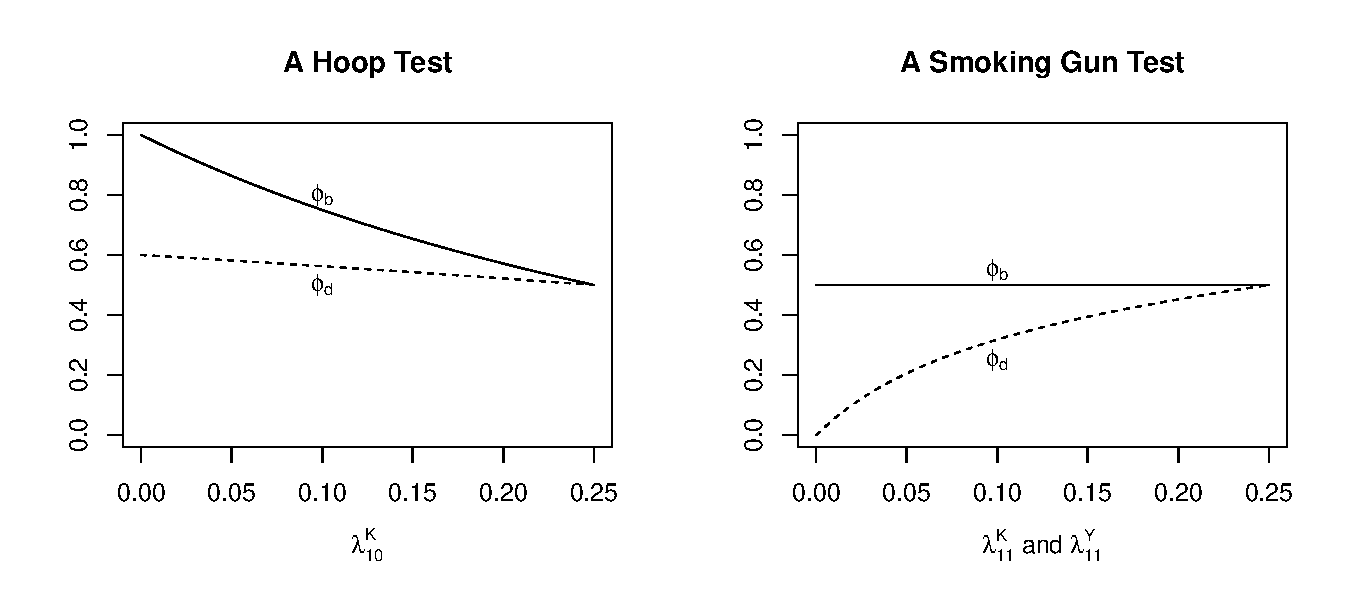
\includegraphics[width=.85\textwidth]{ii_files/figure-latex/phis-1} 

}

\caption{The probability of observing $K$ given causal type for different beliefs on lower-level causal effects. In the left figure, priors on all lower-level causal effects are flat except for the probability that $X$ has a negative effect on $K$. If we believe that it is unlikely that $X$ has a negative effect on $K$, $K$ becomes a `hoop' test for the proposition that a case is of type $b$. The righthand figure considers simultaneous changes in $\lambda_{11}^K$ and  $\lambda_{11}^Y$---the probabilities that $K=1$ regardless of $X$, and that $Y=1$  regardless of $K$, with flat distributions on all other lower-level effects. With $\lambda_{11}^K$, $\lambda_{11}^Y$ both close to 0, $K$ becomes a 'smoking gun' test for the proposition that $X$ has a positive effect on $Y$ ($b$ type).}\label{fig:phis}
\end{figure}

\hypertarget{gains-from-uncertainty}{%
\subsubsection{Gains from uncertainty}\label{gains-from-uncertainty}}

One further implication of this analysis is that sometimes \emph{uncertainty} about causal paths is better than certainty if we seek to generate empirical strategies. If we know for certain that \(X\) always has a positive effect on \(K\) (a mediator), then we learn \emph{nothing} from observing \(K\). We have, in effect, already observed \(K\) once we have observed \(X\). For a mediator clue to convey new information about \(X\)'s effect on \(Y\), we must to some degree start out uncertain about \(X\)'s case-level effect on intervening steps in a causal chain in order for process tracing along the causal chain to be informative about \(X\)'s effect on \(Y\). For learning to occur, there must be uncertainty for \(K\) to resolve. When it comes to using mediators as clues to causal effects, then, strong theories can make for weaker process tracing. This is a general feature of these strategies.

\hypertarget{walk-through-using-a-simple-moderation-model}{%
\subsection{Walk through using a simple moderation model}\label{walk-through-using-a-simple-moderation-model}}

Return now to the moderation example from Chapter 4, graphed here in Figure \ref{fig:modinf}. Here \(Y\) is directly affected by both \(X\) and a second variable, \(K\), which could be a potential clue. As we discuss in Chapter 4, when we theorize moderation of an \(X \rightarrow Y\) effect, we are again partitioning the higher-level response node, \(\theta_Y^{higher}\), into an unobservable \(\theta_Y^{lower}\) and a potentially observable (\(K\)) component. Whereas \(Y\)'s response to \(X\) in the higher-level model is represented by a non-substantive response-node, we have now framed \(Y\)'s response in part in terms of a substantive concept that we believe conditions \(X\)'s effect.

Another important difference between a higher-level \(X \rightarrow Y\) model and a lower-level model of moderation is that \(\theta_Y^{lower}\), in the latter model, determines \(Y\)'s response to \emph{both} \(X\) and \(K\) (whereas \(\theta_Y^{higher}\) only determines \(Y\)'s response to \(X\)). We can think of \(\theta_Y^{lower}\), thus, as fully defining the interaction between \(X\) and \(K\): how, if at all, does \(X\)'s effect depend on \(K\); and how, if at all, does \(K\)'s effect depend on \(X\)?

Using the notation from Chapter 4, we write a value for \(\theta_Y^{lower}\) in a moderation model in the form \(\theta_{ij}^{gh}\), where the four sub- and superscripts provide \(Y\)'s potential outcomes for the four possible combinations of \(X\) and \(K\) values. We arrange the sub- and superscripts to give them an easy visual interpretation, with \(X=0, K=0\) being in the lower lefthand corner (\(i\)); \(X\) going to \(1\) as we move to the right; and \(K\) going to \(1\) as we move up. In other words, a unit has outcome \(i\) when \(X=0, K=0\), \(j\) when \(X=1, K=0\), \(g\) when \(X=0, K=1\), \(h\) when \(X=1, K=1\). \(\theta_Y^{lower}\) in this graph denotes a multinomial distribution over the sixteen possible values of \(\theta_{ij}^{gh}\). We represent all 16 types for \(\theta_Y^{lower}\) in Table \ref{typesmoderation}. Parallel to our notation for mediation, we further represent the population-level shares of the response types as \(\lambda_{ij}^{gh}\).

\begin{table}[h!]
  \centering
  \def\arraystretch{1.3}
    \begin{tabular}{ccccccc}
    \hline
    \textbf {} & \textbf {Type} &  $(Y | X=0,$ & $(Y |X=0, $ & $(Y | X=1, $ & $(Y | X=1, $  & Prior\\
         & & $K=0)$ & $K=1)$ & $K=0)$ & $K=1)$ & ($\lambda_{ij}^{gh}$) \\  \hline
    1 & $\theta_{00}^{00}$          &  0     & 0     & 0     & 0  & 0 \\
    2 & $\theta_{00}^{01}$  & 0     & 0     & 0     & 1 & 0.01 \\
    3 & $\theta_{01}^{00}$  & 0     & 0     & 1     & 0 & 0.2 \\
    4 & $\theta_{01}^{01}$          & 0     & 0     & 1     & 1 & 0.1 \\
    5 & $\theta_{00}^{10}$  & 0     & 1     & 0     & 0 & 0 \\
    6 & $\theta_{00}^{11}$          & 0     & 1     & 0     & 1 & 0.01 \\
    7 & $\theta_{01}^{10}$  & 0     & 1     & 1     & 0 & 0.2 \\
    8 & $\theta_{01}^{11}$      & 0     & 1     & 1     & 1 & 0.2 \\
    9 & $\theta_{10}^{00}$          & 1     & 0     & 0     & 0 & 0 \\
    10 & $\theta_{10}^{01}$     & 1     & 0     & 0     & 1 & 0.01 \\
    11 & $\theta_{11}^{00}$         & 1     & 0     & 1     & 0 & 0.1 \\
    12 & $\theta_{11}^{01}$     & 1     & 0     & 1     & 1 & 0.01 \\
    13 & $\theta_{10}^{10}$         & 1     & 1     & 0     & 0 & 0 \\
    14 & $\theta_{10}^{11}$     & 1     & 1     & 0     & 1 & 0.01 \\
    15 & $\theta_{11}^{10}$     & 1     & 1     & 1     & 0 & 0.1 \\
    16 & $\theta_{11}^{11}$         & 1     & 1     & 1     & 1 & 0.05 \\
    \bottomrule
    \end{tabular}%
   \caption{The table defines the 16 values (response types) that $\theta_Y^{lower}$ can take on, given a binary $X$ and $K$ as parents of $Y$. The `Type' column lists each of the 16 values, while the four columns to its right define each value in terms of the potential outcomes that it implies. The prior represents a possible set of beliefs, before seeing $K$, about the probability that an $X=Y=1$ case is of each type. Rows with a prior of 0 are types that are logically impossible for an $X=Y=1$ case. Row numberings are provided for ease of reference in the text.}
  \label{typesmoderation}%
\end{table}

Suppose, again, that we have observed \(X=Y=1\) in a case and want to know whether \(X=1\) caused \(Y=1\). How can observing \(K\), the moderator, help? In this setup, we can think of learning about \(K\) as shaping inferences through two channels. When we observe a moderator clue, we learn (1) about the laws governing the case and (2) about the case being governed by those laws. Or, mapped onto Figure \ref{typesmoderation}, we learn from a moderator clue both about (1) which row we are in and (2) which pair of columns we are in.

First, observing the moderator clue together with \(X\) provides information about the value of \(\theta_Y^{lower}\)---that is, which row in Figure \ref{typesmoderation} the case belongs to. It tells us something, in other words, about how the case \emph{would} respond in different contingencies. In fact, before we even observe \(K\), we can eliminate rows---values of \(\theta_Y^{lower}\)---based on having observed \(X\), given that we know \(Y\). (This stands to reason, given that \(X\) is \(d\)-connected to \(\theta_Y^{lower}\) by \(Y\).) Specifically, observing \(X=1\) with \(Y=1\) allows us to eliminate any types in which \(Y\) is always \(0\) when \(X=1\): specifically, the types in rows 1, 5, 9, and 13.

Then, observing \(K\) allows us to go further. If we observe, \(K=1\) (having already observed \(X=Y=1\)), then we are now able to rule out additional types: specifically, those in which \(Y=0\) if \(X=K=1\). These are the types in rows 3, 7, 11, and 15. (Alternatively, we if observe \(K=0\), we eliminate any type for which \(Y=0\) when \(X=1\) and \(K=0\), namely the types in rows 2, 6, 10, and 14.)

Thus, the case's possible response types upon observing \(X=Y=K=1\) are those in rows 2, 4, 6, 8, 10, 12, 14, and 16. These types describe the possible `'laws'' governing the case: each indicates \(X\)'s effect in different contexts, as defined by \(K\). The next step is to use \(K\) once more, this time to tell us which context we are in. Since \(K=1\), we know we are in the context represented by the second and fourth columns of potential outcomes.

We can thus ask for which of the eight possible types does \(X\) have a positive causal effect when \(K=1\) (i.e., restricting to the second and fourth columns of potential outcomes). These are the types in rows 2, 4, 10, and 12: \(\theta_{00}^{01}\), \(\theta_{01}^{01}\), \(\theta_{10}^{01}\), and \(\theta_{11}^{01}\). In rows 6 (\(\theta_{00}^{11}\)), 8 (\(\theta_{01}^{11}\)), 14 (\(\theta_{10}^{11}\)), and 16 (\(\theta_{11}^{11}\)), \(X\) has zero effect. Thus, for half of the types consistent with the data, \(X\) has a positive effect on \(Y\), and for half \(Y\) would have been \(1\) regardless of \(X\)'s value.

As for a mediator clue, we need to draw on prior beliefs over the causal possibilities in order to learn from the moderator clue. To help us think through how such beliefs might operate in this setting, let us return to our running example. Suppose that \(X\) is the presence of a free press, \(K\) is a measure of government sensitivity to public opinion, and \(Y\) is government removal. Let us suppose that we do not know the structural equations connecting the variables (i.e., we bracket those presented in Chapter 2). However, based on previous research, we have beliefs over causal possibilities.

In the final column of Table \ref{typesmoderation}, we provide a set of priors representing a possible set of such beliefs. Broadly, the priors we use for this illustration represent a few intuitive beliefs about the causal relationships in play: that the free press will represent a threat to governments that are insensitive to public opinion; that a free press could plausibly reinforce the legitimacy and thus prevent the removal of a government sensitive to public opinion (i.e., could have the opposite effect for a sensitive and an insensitive government); that a free press rarely prevents government removal when the government is insensitive to public opinion; that sensitivity of the government to public opinion rarely causes government removal; that it is not unlikely that the free press has no effect, regardless of sensitivity; and that it is somewhat likely that \emph{neither} a free press nor sensitivity has no effect, regardless of the other. Types excluded by the \(X, Y\) data alone are given a prior weight of 0 since we know that they are impossible before we observe the clue.

Given these priors, we can readily calculate our prior confidence---based just on the \(X=Y=1\) observation---that the free press caused government removal (i.e., that the higher-level type is \(\theta_{01}\). This is the population share represented by those types for which \(X\) has a positive effect on \(Y\) at some value of \(K\), with each type weighted in the calculation by the probability that \(K\) in fact takes on that value under which that type displays a positive effect of \(X\) on \(Y\).\footnote{\[P(i \in t_{01} | X=Y=1) = \frac{
  \pi^K\left(\lambda_{00}^{01}+\lambda_{10}^{01}+\lambda_{01}^{01}+\lambda_{11}^{01}\right)
  +
  (1-\pi^K)\left(\lambda_{01}^{00}+\lambda_{01}^{10}+\lambda_{01}^{01}+\lambda_{01}^{11}\right)
  }{
  \sum_{i = 0}^1\left(\pi^K\left(\lambda_{00}^{i1}+\lambda_{10}^{i1}+\lambda_{01}^{i1}+\lambda_{11}^{i1}\right)
  +
  (1-\pi^K)\left(\lambda_{i1}^{00}+\lambda_{i1}^{10}+\lambda_{i1}^{01}+\lambda_{i1}^{11}\right)
  \right)}\]} Thus, to calculate our prior on the causal effect of \(X\), we need to also set a prior on how commonly we think governments (in cases with a free press and government removal) are sensitive to public opinion (\(\pi^K\) from our original causal model). Here we set the prior probability of \(K=1\) to 0.5.

Using our specified prior beliefs, our prior confidence that the free press caused government removal is 0.61. Now, what happens if we go and collect our clue, measuring government sensitivity? If we look for the clue and find it (\(K=1\)), then our posterior probability becomes the population share of those types consistent with \(X=Y=K=1\) for which \(X\) has a positive effect on \(Y\) when \(K\) in fact is \(1\).\footnote{\(P(i \in t_{01} | X=Y=1, K=1) = \frac{\left(\lambda_{00}^{01}+\lambda_{10}^{01}+\lambda_{01}^{01}+\lambda_{11}^{01}\right)}{\sum_{i = 0}^1\left(\lambda_{00}^{i1}+\lambda_{10}^{i1}+\lambda_{01}^{i1}+\lambda_{11}^{i1}\right)}\)} (We can see in this statement the learning both about which the laws governing the case's responses to context and about the context that the case is in.) This share works out to 0.325. Thus, if we observe a sensitive government, we become much less confident that \(X\) caused \(Y\) in this case. On the other hand, if we measure the government's sensitivity and find that it is insensitive (\(K=0\)), our confidence that \(X\) caused \(Y\) goes \emph{up} somewhat to 0.73.\footnote{\(P(i \in t_{01} | X=Y=1, K=0) = \frac{\left(\lambda_{01}^{00}+\lambda_{01}^{10}+\lambda_{01}^{01}+\lambda_{01}^{11}\right)}{\sum_{i = 0}^1\left(\lambda_{i1}^{00}+\lambda_{i1}^{10}+\lambda_{i1}^{01}+\lambda_{i1}^{11}\right)}\)} Thus, the search for governmental insensitivity functions as a relatively easy hoop test for the proposition that the free press caused the government's removal.

\begin{figure}

{\centering 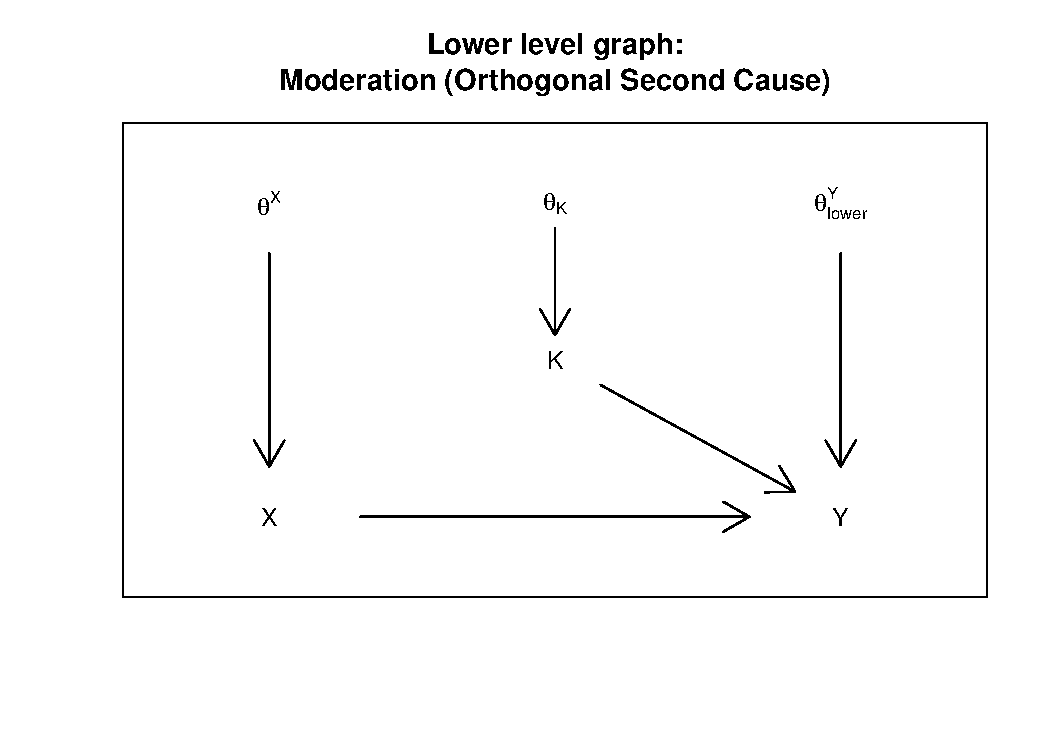
\includegraphics[width=.7\textwidth]{ii_files/figure-latex/unnamed-chunk-35-1} 

}

\caption{\label{fig:modinf} A model with one explanatory variable and one moderator.}\label{fig:unnamed-chunk-35}
\end{figure}

\hypertarget{connection-to-qualitative-tests-1}{%
\subsubsection{Connection to qualitative tests}\label{connection-to-qualitative-tests-1}}

Again we can undertake this analysis by calculating \(\phi\) values as used in \citet{humphreys2015mixing}: that is, the probability of observing a clue, \(K\), if a given proposition is true. Since we have already observed \(X=Y=1\) in the case, the \(phi\) values of interest here are \(\phi_{t_{01}1}\) and \(\phi_{t_{11}1}\): the probability of observing the clue for an \(X=1\) case of type \(\theta_{01}\) (a \(b\) type, or positive effect) and the probability of observing the clue for an \(X=1\) case of type \(\theta_{11}\) (a \(d\) type, or zero effect). By assumption in the lower-level model, \(K\) is as-if randomly assigned: in particular (without conditioning on \(Y\)), \(K\) is orthogonal to \(\theta_Y^{lower}\)---that is, to \(Y\)'s responsiveness to \(K\). While the probability of observing \(K\) is thus the same for all lower-level \(Y\) types, that probability is---critically---not the same for all the types in the \emph{higher}-level theory. The higher-level types---those of interest for determining \(X\)'s effect on \(Y\)---are themselves related to the probability of \(K\). Moreover, \(K\) is also correlated with the \emph{lower}-level type variable, \(\theta_Y^{lower}\), \emph{conditional} on \(Y\). In particular, given \(Y=1\), we can calculate the probability of observing the clue if \(X=1\) and the case is of type \(\theta_{j1}\) as:

\[\phi_{t_{j1}1} = \frac{\pi^K\left(\lambda_{00}^{j1}+\lambda_{10}^{j1}+\lambda_{01}^{j1}+\lambda_{11}^{j1}\right)}{\pi^K\left(\lambda_{00}^{j1}+\lambda_{10}^{j1}+\lambda_{01}^{j1}+\lambda_{11}^{j1}\right)
+
(1-\pi^K)\left(\lambda_{j1}^{00}+\lambda_{j1}^{10}+\lambda_{j1}^{01}+\lambda_{j1}^{11}\right)}\]

\hypertarget{illustration-with-code}{%
\subsection{Illustration with code}\label{illustration-with-code}}

\begin{Shaded}
\begin{Highlighting}[]
\NormalTok{model <-}\StringTok{ }\KeywordTok{make_model}\NormalTok{(}\StringTok{"X -> Y <- K"}\NormalTok{) }\OperatorTok
\StringTok{         }\KeywordTok{set_parameters}\NormalTok{(}\KeywordTok{c}\NormalTok{(.}\DecValTok{5}\NormalTok{, }\FloatTok{.5}\NormalTok{, }\FloatTok{.5}\NormalTok{, }\FloatTok{.5}\NormalTok{, }
                          \DecValTok{0}\NormalTok{,}\DecValTok{1}\OperatorTok{/}\DecValTok{3}\NormalTok{,}\DecValTok{0}\NormalTok{,}\DecValTok{0}\NormalTok{,}\DecValTok{0}\NormalTok{,}\DecValTok{0}\NormalTok{,}\DecValTok{0}\NormalTok{,}\DecValTok{0}\NormalTok{,}
                          \DecValTok{1}\OperatorTok{/}\DecValTok{3}\NormalTok{,}\DecValTok{0}\NormalTok{,}\DecValTok{0}\NormalTok{,}\DecValTok{0}\NormalTok{,}\DecValTok{0}\NormalTok{,}\DecValTok{0}\NormalTok{,}\DecValTok{0}\NormalTok{,}\DecValTok{1}\OperatorTok{/}\DecValTok{3}\NormalTok{)) }

\KeywordTok{get_estimands}\NormalTok{(}
\NormalTok{    model, }
    \DataTypeTok{queries =} \KeywordTok{list}\NormalTok{(}\DataTypeTok{COE =} \StringTok{"Y[X=1] > Y[X=0]"}\NormalTok{), }
    \DataTypeTok{subsets =} \KeywordTok{list}\NormalTok{(}\StringTok{"X==1 & Y==1"}\NormalTok{, }\StringTok{"X==1 & Y==1 & K==0"}\NormalTok{, }\StringTok{"X==1 & Y==1 & K==1"}\NormalTok{),}
    \DataTypeTok{using =} \StringTok{"parameters"}\NormalTok{)}
\end{Highlighting}
\end{Shaded}

\begin{verbatim}
## Warning: 
## The get_estimands function has been renamed draw_estimands, to make clear that the estimands are draws from a simulation. Please replace your code with draw_estimands.
\end{verbatim}

\hypertarget{four-principles}{%
\section{Four principles}\label{four-principles}}

\hypertarget{conditional-independence-alone-does-not-provide-probative-value}{%
\subsection{Conditional independence alone does not provide probative value}\label{conditional-independence-alone-does-not-provide-probative-value}}

\hypertarget{uncertainty-does-not-alter-inference-for-single-case-causal-inference}{%
\subsection{Uncertainty does not alter inference for single case causal inference}\label{uncertainty-does-not-alter-inference-for-single-case-causal-inference}}

\hypertarget{probative-value-requires-d-connection}{%
\subsection{\texorpdfstring{Probative value requires \(d-\)connection}{Probative value requires d-connection}}\label{probative-value-requires-d-connection}}

As we have argued, causal estimands can be expressed as the values of exogenous nodes in a causal graph. Case-level causal effects and causal paths can be defined in terms of response-type nodes; average effects and notable causes in terms of population-level parameter nodes (e.g., \(\pi\) or \(\lambda\) terms); and questions about actual causes in terms of exogenous conditions that yield particular endogenous values (conditioning on which makes some variable a counterfactual cause).

We thus define causal inference more generally as \emph{the assessment of the value of one or more unobserved (possibly unobservable) exogenous nodes on a causal graph, given observable data.} To think through the steps in this process, it is useful to distinguish among three different features of the world, as represented in our causal model: there are the things we want to learn about; the things we have already observed; and the things we could observe. As notation going forward, let:

\begin{itemize}
\tightlist
\item
  \(\mathcal Q\) denote the exogenous variables that define our \emph{query}; we generally assume that \(\mathcal Q\) cannot be directly observed so that its values must be inferred
\item
  \(\mathcal W\) denote a set of previously observed nodes in the causal model, and
\item
  \(\mathcal K\) denote a set of additional variables---clues---that we have not yet observed but could observe.
\end{itemize}

Now suppose that we seek to design a research project to investigate a causal question. How should the study be designed? Given that there are some features of the world that we have already observed, which additional clues should we seek to collect to shed new light on our question? In terms of the above notation, what we need to figure out is whether a given \(\mathcal K\) might be informative about---might provide additional leverage on---\(\mathcal Q\) given the prior observation of \(\mathcal W\).

To ask whether one variable (or set of variables) is informative about another is to ask whether the two (sets of) variables are, on average, \emph{correlated} with one another, given whatever we already know. Likewise, if two variables' distributions are fully \emph{independent} of one another (conditional on what else we have observed), then knowing the value of one variable can provide no new information about the value of the other.

Thus, asking whether a set of clues, \(\mathcal K\), is informative about \(\mathcal Q\) given the prior observation of \(\mathcal W\), is equivalent to asking whether \(\mathcal K\) and \(\mathcal Q\) are conditionally independent given \(\mathcal W\). That is, \(\mathcal K\) can be informative about \(\mathcal Q\) given \(\mathcal W\) only if \(\mathcal K\) and \(\mathcal Q\) are \emph{not} conditionally independent of one another given \(\mathcal W\).

As we have shown, as long as we have built \(\mathcal Q\), \(\mathcal K\), and \(\mathcal W\) into our causal model of the phenomenon of interest, we can answer this kind of question by inspecting the structure of the model's DAG. In particular, what we need to go looking for are relationships of \emph{\(d\)-separation}. The following proposition, with only the names of the variable sets altered, is from \citet{pearl2009causality} (Proposition 1.2.4):

\textbf{Proposition 1:} If sets \(\mathcal Q\) and \(\mathcal K\) are \(d\)-separated by \(\mathcal W\) in a DAG, \(\mathcal G\), then \(\mathcal Q\) is independent of \(\mathcal K\) conditional on \(\mathcal W\) in every distribution compatible with \(\mathcal G\). Conversely, if \(\mathcal Q\) and \(\mathcal K\) are \emph{not} \(d\)-separated by \(\mathcal W\) in DAG \(\mathcal W\), then \(\mathcal Q\) and \(\mathcal K\) are dependent conditional on \(\mathcal W\) in at least one distribution compatible with \(\mathcal G\).

We begin with a causal graph and a set of nodes on the graph (\(W\)) that we have already observed. Given what we have already observed, \emph{a collection of clue nodes, \(\mathcal K\), will be uninformative about the query nodes, \(\mathcal Q\), if \(\mathcal K\) is \(d\)-separated from \(\mathcal Q\) by \(\mathcal W\) on the graph.} When \(\mathcal W\) \(d\)-separates \(\mathcal K\) from \(\mathcal Q\), this means that what we have already observed already captures all information that the clues might yield about our query. On the other hand, if \(\mathcal K\) and \(\mathcal Q\) are \(d\)-connected (i.e., not \(d\)-separated) by \(W\), then \(K\) is \emph{possibly} informative about \(Q\).\(K\) is not \(d\)-separated from \(\mathcal Q\) by \(\mathcal W\).\footnote{This proposition is almost coextensive with the definition of a DAG. A DAG is a particular kind of dependency model (``graphoid'') that is a summary of a collection of ``independency statements'', \((I)\), over distinct subsets of \(\mathcal V\) (Pearl and Verma 1987), where \(I(\mathcal Q,\mathcal W,\mathcal K)\) means ``we learn nothing about \(\mathcal Q\) from \(\mathcal K\) if we already know \(\mathcal W\)''. More formally:
  \[I(\mathcal K, \mathcal W,\mathcal Q) \leftrightarrow P(\mathcal K,\mathcal Q|\mathcal W)=P(\mathcal K|\mathcal W)P(\mathcal Q|\mathcal W)\]
  A Directed Acyclic Graph Dependency model is one where the set of independencies correspond exactly to the relations that satisfy \(d\)-separation (Pearl and Verma 1987, p376). Thus on DAG \(\mathcal G\), \(I(\mathcal K,\mathcal W,\mathcal Q)_\mathcal G\) implies that \(\mathcal K\) and \(\mathcal Q\) are \(d\)-separated by \(\mathcal W\).} Note, moreover, that under quite general conditions (referred to in the literature as the \emph{faithfulness} of a probability distribution) then there are at least \emph{some} values of \(\mathcal W\) for which \(\mathcal K\) \emph{will} be informative about \(\mathcal Q\).\footnote{Put differently, there will not be any conditional independencies that are \emph{not} captured in the DAG.}

Let us examine Proposition 1 in practice. We begin with the simplest case possible, and then move on to more complex models.

The very simplest probabilistic causal graph has \(X\) influencing \(Y\), with \(X\) determined by a coin flip. Assuming that there is some causal heterogeneity---that is, it is unknown in any particular case whether \(X\) causes \(Y\)---we also include a response-type variable, \(Q\), pointing into \(Y\), as shown in Figure \ref{fig:d-sepsimple}. Here, \(Q^Y\) determines the value of \(Y\) that will be generated by \(X\). Asking about the causal effect of \(X\) in a case thus means learning the value of \(Q^Y\) in that case. As will be recalled, in a binary setup with one causal variable, a response-type variable can take on one of four values, \(q^Y_{00}\), \(q^Y_{10}\), \(q^Y_{01}\) and \(q^Y_{11}\),\footnote{As a reminder, we read \(q^Y_{ij}\) (when \(X\) is binary) as meaning that \(Y\) will take on value \(i\) when \(X=0\) and value \(j\) when \(X=1\).} corresponding to the four possible causal types in this setting.

\begin{figure}

{\centering 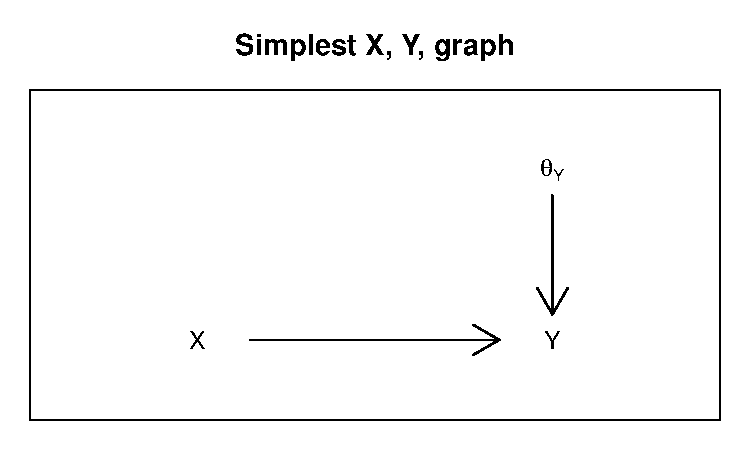
\includegraphics[width=.5\textwidth]{ii_files/figure-latex/unnamed-chunk-37-1} 

}

\caption{\label{fig:d-sepsimple} A simple causal setup in which the effect of $X$ on $Y$ in a given case depends on the case's response type for $Y$.}\label{fig:unnamed-chunk-37}
\end{figure}

Let us assume that we have observed nothing yet in this case and then ask what clue(s) might be informative about \(Q^Y\), the node of interest. The other two nodes in the graph are \(X\) and \(Y\): these are thus the possible clues that we might go looking for in our effort to learn about \(Q^Y\) (i.e., they are the possible members of \(\mathcal K\)).

First, can we learn about \(Q^Y\) by observing \(X\)? We can answer this question by asking whether \(X\) is \(d\)-connected to \(Q^Y\) on the graph given what we have already observed (which is nothing). We can see visually that there is no active path from \(X\) to \(Q^Y\): the only path between \(X\) and \(Q\) is blocked by colliding arrow heads. Thus, \(X\) and \(Q^Y\) are \(d\)-separated, meaning that \(X\) will not be informative about \(Q^Y\): observing the value that a causal variable takes on in a case---having seen nothing else in the case---tells us nothing whatsoever about that variable's effect on the outcome. If we want to know whether a case is of a type in which the presence of natural resources would cause civil war, observing only that the case has natural resources does not help answer the question.

--\textgreater{}

What, then, if we instead were to observe only \(Y\)? Is \(Y\) \(d\)-connected to \(Q\) given what we have already observed (which, again, is nothing)? It is: the arrow from \(Q^Y\) to \(Y\) is an active path. Observing only the \emph{outcome} in a case does tell us something about causal effects. Returning to the natural resources and civil war example, observing only that a country has had a civil is informative about the case's causal type (the value of \(Q^Y\)). In particular, it rules out the possibility that this is a case in which nothing could cause a civil war: that is, it excludes \(q^Y_{00}\) (i.e., \(c\)-type) as a possible value of \(Q^Y\).

Suppose now, having observed \(Y\), that we were to consider also observing \(X\). Would we learn anything further about \(Q^Y\) from doing so? We have already seen that observing \(X\) alone yields no information about \(Q^Y\) because the two nodes are unconditionally \(d\)-separated, the path between them blocked by the colliding arrowheads at \(Y\). However, as we have seen, observing a collider variable (or one of its descendants) \emph{unblocks} the flow of information, generating relations of conditional dependence across the colliding arrowheads. Here, \(X\) and \(Q^Y\) are \(d\)-connected by \(Y\): thus, if we have \emph{already} observed \(Y\), then observing \(X\) does confer additional information about \(Q^Y\). Knowing only that a country has natural resources tells us nothing about those resources' effect on civil war in that country. But if we already know that the country has a civil war, then learning that the country has natural resources helps narrow down the case's possible response types. Having already used the observation of \(Y=1\) to rule out the possibility that \(Q^Y=q^Y_{00}\), observing \(X=1\) \emph{together with} \(Y=1\) allows us to additionally rule out the possibility that natural resources \emph{prevent} civil war, i.e., that \(Q^Y=q^Y_{01}\).\footnote{That is, we can rule out that the case is an \(a\) type, or one with a negative causal effect.}

Finally, what if we observe \(X\) first and are considering whether to seek information about \(Y\)? Would doing so be informative? \(X\) does not \(d-\)separate \(Q^Y\) from \(Y\); thus, observing \(Y\) will be informative about \(Q^Y\). In fact, observing \(Y\) if we have already seen \(X\) is \emph{more} informative than observing \(Y\) alone. The reasoning follows the logic of collision discussed just above. If we observe \(Y\) having already seen \(X\), not only do we reap the information about \(Q^Y\) provided by \(Y\)'s correlation with \(Q^Y\); we simultaneously open up the path between \(X\) and \(Q^Y\), learning additionally from the conditional dependence between \(X\) and \(Q^Y\) given \(Y\).

We put Proposition 1 to work in a slightly more complex set of models in Figure \ref{fig:34graphs}. Here we investigate the informativeness of a clue that is neither \(X\) nor \(Y\). Each graph in Figure \ref{fig:34graphs} has four variables: \(X\); \(Y\); a possible clue, \(K\); and a response-type variable, \(Q\). We draw all 34 possible graphs with variables \(X\), \(Y\), \(K\), and \(Q\) for causal models in which (a) all variables are connected to at least one other variable, (b) \(X\) causes \(Y\) either directly or indirectly, and (c) \(Q\) is a direct cause of \(Y\) but is not caused by any other variable in the model and is thus exogenous. The title of each panel reports \(K\)'s conditional informativeness using principles of \(d\)-separation: it tells us when \(K\) is possibly informative about \(Q\) depending on whether \(X\), \(Y\), both or none are observed.\footnote{Note the ``possibly'' can be dropped under the assumption that the underlying probability model is ``stable'' (Pearl 2009, section 2.9.1) and with the interpretation that \(K\) is informative about \(Q\) for some, but not necessarily all, values of \(W\).}

\begin{figure}
\centering
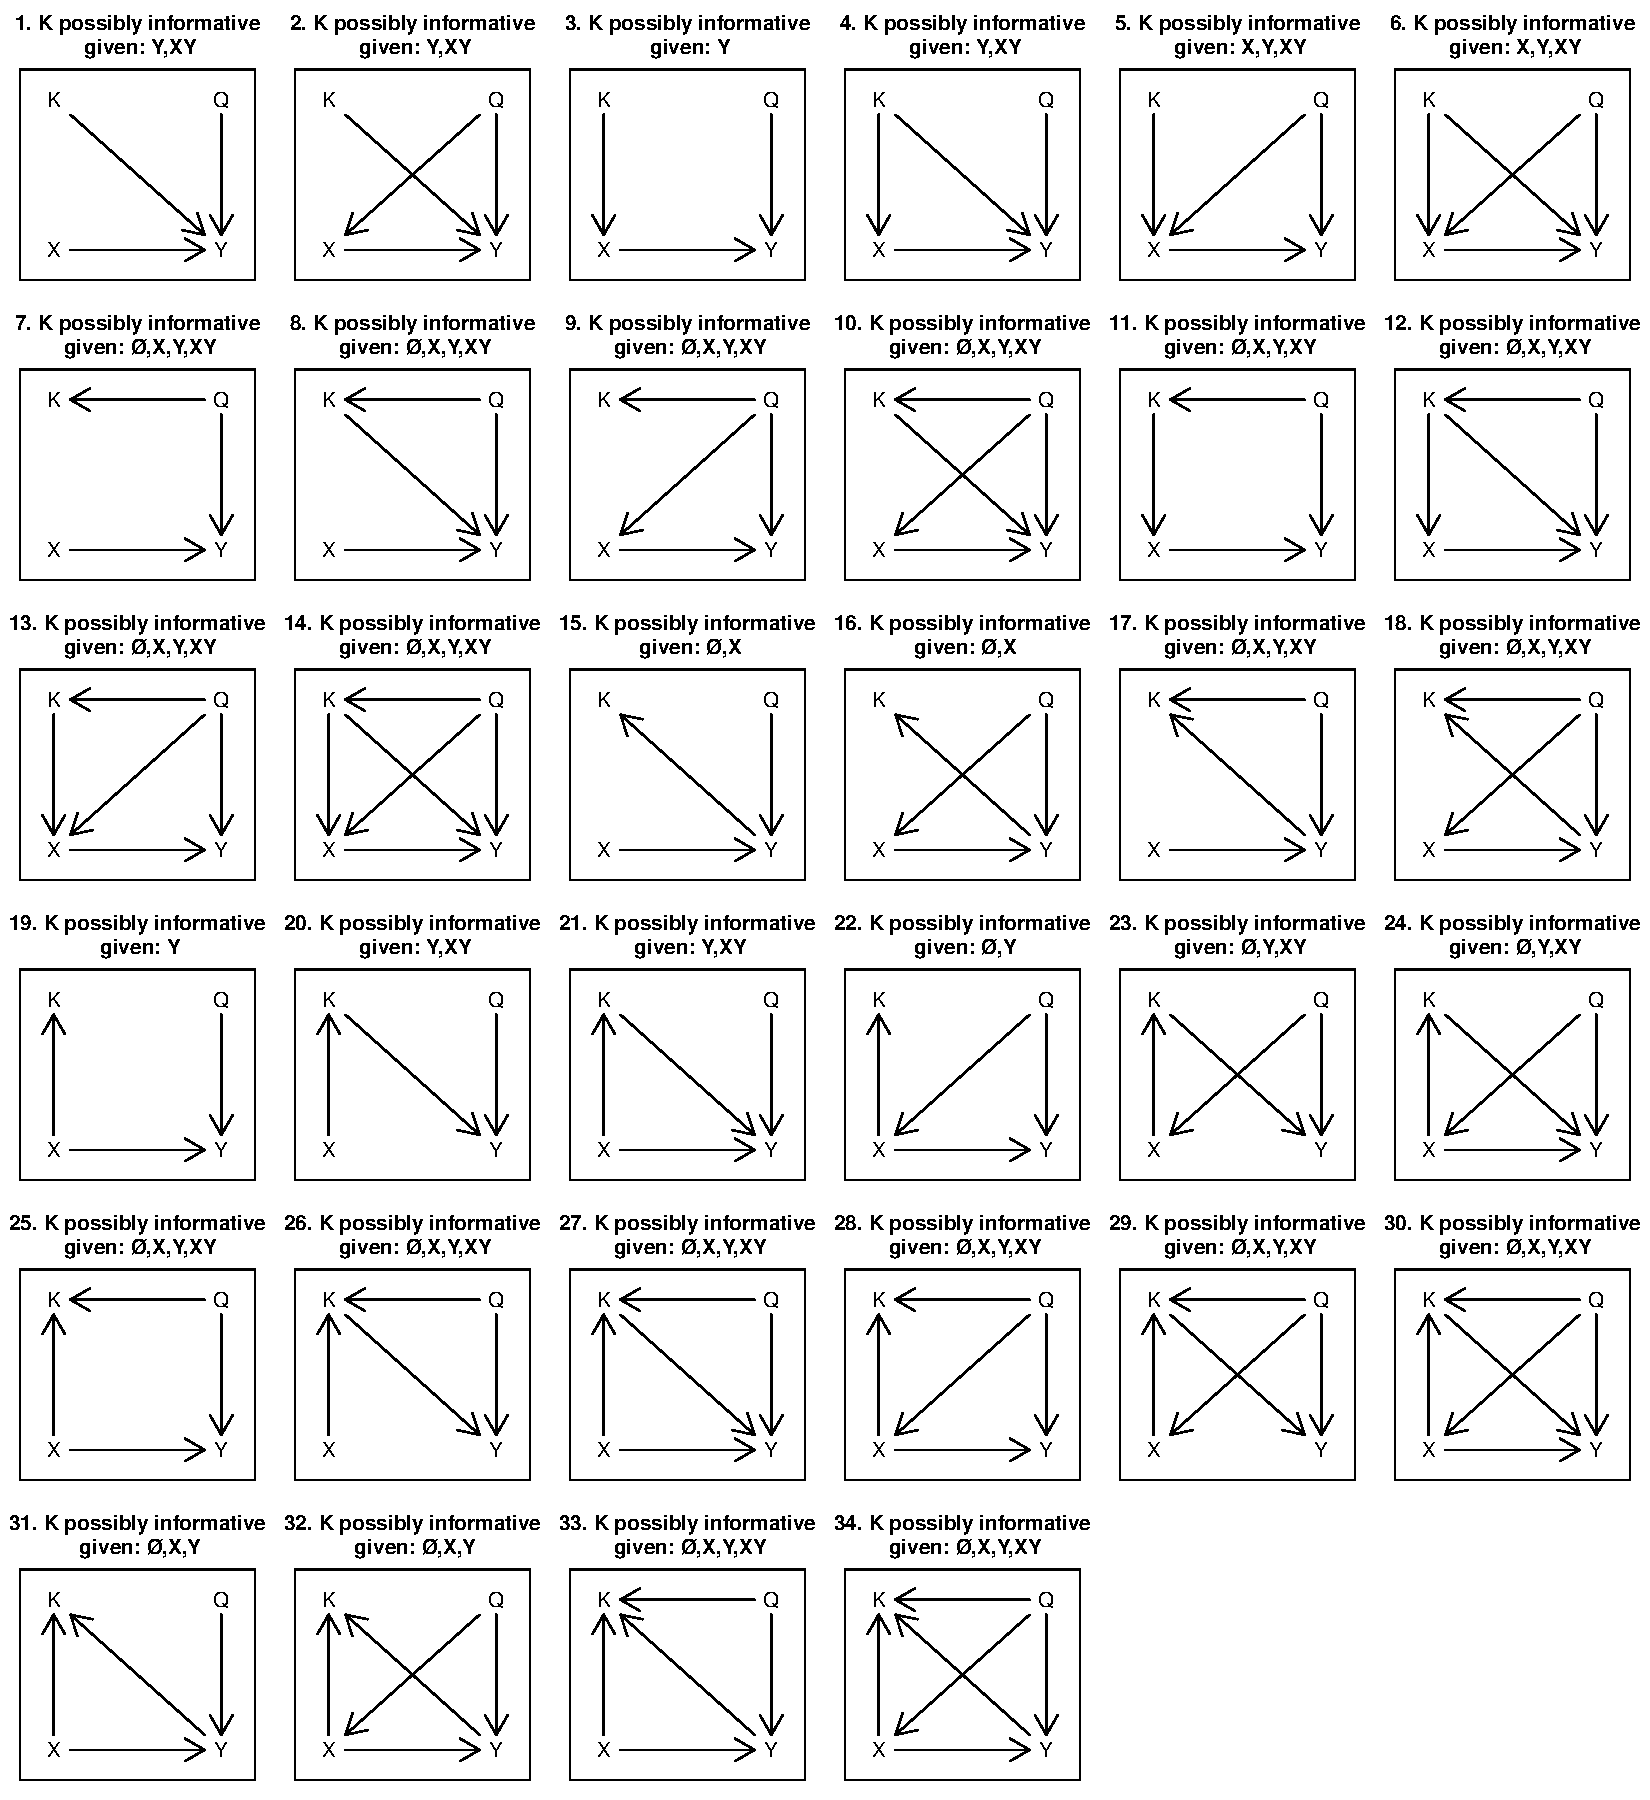
\includegraphics{ii_files/figure-latex/unnamed-chunk-39-1.pdf}
\caption{\label{fig:unnamed-chunk-39}\label{fig:34graphs} All connected directed acyclic graphs over \(X,Y,K,Q\), in which \(Q\) is an exogenous variable that directly causes \(Y\), and \(X\) is a direct or indirect cause of \(Y\). The title of each graph indicates the conditions under which \(K\) can be informative about (i.e., is not \(d\)-separated from) \(Q\), given the prior observation of \(X\), \(Y\), both, or neither (\ldots{}).}
\end{figure}

\hypertarget{probative-value}{%
\subsection{Probative value}\label{probative-value}}

The results show us not just what kinds of variables can be informative about a case's response-type but also what combinations of observations yield leverage on case-level causal effects. A number of features the graphs are worth highlighting:

\begin{itemize}
\item
  \textbf{Clues at many stages.} Process tracing has focused a great deal on observations that lie ``along the path'' between suspected causes and outcomes. What we see in Figure \ref{fig:34graphs}, however, is that observations at many different locations in a causal model can be informative about causal effects. We see here that \(K\) can be informative when it is pre-treatment (causally prior to \(X\)---e.g.~panel (3)), post-treatment but pre-outcome (that is, ``between'' \(X\) and \(Y\) as, e.g., in panel (20)), an auxiliary effect of \(X\) that itself has no effect on \(Y\) (e.g., in panel (19)), post-outcome (after \(Y\)---e.g., in panel (15)), or a joint effect of both the suspected cause and the outcome (e.g., panel (31)).
\item
  \textbf{Mediator Clues}. While clues that lie in between \(X\) and \(Y\) may be informative, they can only be informative under certain conditions. For instance, when a clue serves \emph{only} as a mediator in our model (i.e., its only linkages are being caused by \(X\) and being affected by \(Y\)) and \(Q\) only affects \(Y\), as in panels (20) and (21), the clue is only informative about \(Q\) if we have also observed the outcome, \(Y\). Of course, this condition may commonly be met---qualitative researchers usually engage in retrospective research and learn the outcome of the cases they are studying early on---but it is nonetheless worth noting why it matters: in this setup, \(K\) is unconditionally \(d\)-separated from \(Q\) by the collision at \(Y\); it is only by observing \(Y\) (the collider) that the path between \(K\) and \(Q\) becomes unblocked. (As we saw above, the very same is true for observing \(X\); it is only when we know \(Y\) that \(X\) is informative about \(Q\).)
\end{itemize}

In short, observations along causal paths are more helpful in identifying causal effects to the extent that we have measured the outcome. Importantly, this is not the same as saying that mediator clues are \emph{only} informative about causal effects where we have observed the outcome. Observing \(Y\) is necessary for the mediator to be informative about a \(Q\) term that is connected only to \(Y\). Observing a mediator without the outcome, however, could still be informative about the overall effect of \(X\) on \(Y\) by providing leverage on how the mediator responds to \(X\), which is itself informative about \(X\)'s effect on \(Y\) via the mediator.\footnote{In other words, the clue would then be providing leverage on a response-type variable pointing into the mediator itself.} Moreover, observing the mediator could be informative without the observation of \(Y\) if, for instance, \(Q\) also points into \(K\) itself or into a cause of \(K\). As we discuss below, the clue then is informative as a ``symptom'' of the case's response type, generating learning that does not hinge on observing the outcome.

\begin{itemize}
\tightlist
\item
  \textbf{Symptoms as clues.} Some clues may themselves be affected by \(Q\): that is to say, they may be symptoms of the same conditions that determine causal effects in a case. For instance, in our illustrative model involving government survival, government sensitivity functions as a response-type variable for the effect of a free press (\(X\)) on government removal (\(Y\)): a free press only generates government removal when the government is non-sensitive to public opinion. Sensitivity to public opinion thus represents our query variable, \(Q\), if we seek to learn whether a free press causes government removal in a case. While it may not be possible to observe or otherwise measure the government's sensitivity, there may be \emph{consequences} of government sensitivity that are observable: for instance, whether government officials regularly consult with civil-society actors on policy issues. While consultations would not be part of the causal chain generating the free press's effect, observing consultations (or the lack of them) would be informative about that effect because consultations are a symptom of the same conditions that enable the effect.
\end{itemize}

We see that \(K\) is a child or descendant of \(Q\) in several of the graphs in Figure \ref{fig:34graphs}: \(Q\) directly causes \(K\) in panels (7) through (14), (17), (18), (25)-(30), (33), and (34); \(Q\) causes (K) only indirectly through \(X\) in panels (22) through (24); \(Q\) causes (K) only indirectly through \(Y\) in panels (15), (16), and (31); and \(Q\) causes \(K\) only indirectly through \(X\) and through \(Y\) in panel (32). We can then use the principle of \(d\)-separation to figure out when the symptom clue is potentially informative, given what we have already observed. It is easy to see that \(K\) is potentially informative, no matter what we have already observed, if \(K\) is directly affected by \(Q\); there is nothing we could observe that would block the \(Q \rightarrow K\) path. Thus, \(Q\)'s ``symptom'' can, in this setup, contain information about type above and beyond that contained in the \(X\) and \(Y\) values. However, where \(Q\) affects \(K\) only through some other variable, observing that other variable renders \(K\) uninformative by blocking the \(Q\)-to-\(K\) path. For instance, where \(Q\) affects \(K\) indirectly through \(X\), once we observe \(X\), we already have all the information about \(Q\) that would be contained in \(K\).

\begin{itemize}
\tightlist
\item
  \textbf{Surrogates as clues.} Clues may be consequences of the outcome, as in graphs (15) and (16). If \(K\) is a consequence \emph{only} of \(Y\), then it will contain no new information about \(Q\) where \(Y\) is already known. However, in situations where the outcome has not been observed, \(K\) can act as a ``surrogate'' for the outcome and thus yield leverage on \(Q\) (\citet{frangakis2002principal}). A researcher might, for instance, seek to understand causal effects on an outcome that is difficult to directly observe: consider, for instance, studies that seek to explain ideational change. Ideas themselves, the \(Y\) in such studies, are not directly observable. However, their consequences---such as statements by actors or policy decisions---will be observable and can thus serve as informative surrogates for the outcome of interest.
\end{itemize}

Clues may similarly serve as surrogates of a cause, as in graphs (19) and (22). Here \(X\) causes \(K\), but \(K\) plays no role in the causal process generating \(Y\). \(K\) is of no help if we can directly measure \(X\) since the latter \(d\)-separates \(K\) from \(Q\). But if an explanatory variable cannot be directly measured---consider, e.g., ideas or preferences as causes---then its consequences, including those that have no relationship to the outcome of interest, can provide leverage on the case-level causal effect.

Clues can also be a consequence of both our suspected cause and the outcome of interest, thus serving as what we might call ``double surrogates,'' as in panels (31) and (32). Here \(X\) is a direct cause of \(Y\), and \(K\) is a joint product of \(X\) and \(Y\). A double surrogate can be informative as long as we have not already observed both \(X\) and \(Y\). Where data on either \(X\) or \(Y\) are missing, there is an open path between \(K\) and \(Q\). If we have already observed both, however, then there is nothing left to be learned from \(K\).

\begin{itemize}
\tightlist
\item
  \textbf{Instruments as clues.} Clues that are causally prior to an explanatory variable, and have no other effect on the outcome, can sometimes be informative. Consider, for instance, graph (3). Here \(K\) is the only cause of \(X\). It can thus serve as a proxy. If we have seen \(X\), then \(X\) blocks the path between \(K\) and \(Q\), and so \(K\) is unhelpful. \(K\) can be informative, though, if we have \emph{not} observed \(X\). Note that informativeness here still requires that we observe \(Y\). Since \(Y\) is a collider for \(Q\) and the \(K \rightarrow X \rightarrow\) chain, we need to observe \(Y\) in order to \(d\)-connect \(K\) to \(Q\).
\end{itemize}

A rather different setup appears in graph (5), where both \(K\) and \(Q\) cause \(X\). Now the conditions for \(K\)'s informativeness are broader. Observing \(X\) still makes \(K\) uninformative as a proxy for \(X\) itself. However, because \(X\) is a collider for \(K\) and \(Q\), observing \(X\) \emph{opens up} a path from \(K\) to \(Q\), rendering a dependency between them. Still, we have to observe at least one of \(X\) or \(Y\) for the instrument to be informative here. This is because both of \(K\)'s paths to \(Q\) run through a collision that we need to unblock by observing the collider. For one path, the collider is \(X\); for the other path, the collider is \(Y\).\footnote{As a simple example one might imagine a system in which \(X = K\) if \(q \in {a,b}\) and \(X = 1-K\) if \(q \in {c,d}\). Then if we observe, say, \(X=Y=K=1\), we can infer that \(q = b\). Another way to think about what is happening in graph (5) is that \(K\) is providing information about the \emph{assignment process}. In this graph, the causal effect (\(Y\)'s potential outcomes, determined by \(Q\)) is also a partial determinant of the assignment of cases to values on \(X\). In terms of cross-case correlational inference, then, we would think of this as a situation of confounding. Observing another cause of \(X\), then, allows us to more fully characterize the process of assignment.}

Other patterns involving instrumentation are also imaginable, though not graphed here. For example, we might have a causal structure that combines instrumentation and surrogacy. Suppose that \(X\) is affected by \(Q\) and by an unobservable variable \(\theta_X\); and that \(\theta_X\) has an observable consequence, \(K\). Then \(K\), though not a cause of \(X\), is a ``surrogate instrument'' \citep{hernan2006instruments} as it is a descendant of an unobserved instrument, \(U\), and thus allows us to extract inferences similar to those that we could draw from a true instrument.

\begin{itemize}
\tightlist
\item
  \textbf{Confounders as clues.} In several of the graphs, \(K\) is a confounder in that it is a direct cause of both \(X\) and \(Y\) (panels (4), (6), (12), and (14)). Let us focus on graph (4), which isolates \(K\)'s role as a confounder. Here \(K\) can be informative via two possible paths. First, if \(X\) is not observed but \(Y\) is, then \(K\) is \(d\)-connected to \(Q\) along the path \(K \rightarrow X \rightarrow Y \leftarrow Q\). \(K\) is in this sense serving as a proxy for \(X\), with its path to \(Q\) opened up by the observation of the collider, \(Y\). Second, with \(Y\) observed, \(K\) can provide information on \(Q\) via the more direct collision, \(K \rightarrow Y \leftarrow Q\). If \(X\) \emph{is} observed, then the first path is blocked, but the second still remains active. As with any pre-outcome variable, for a confounder clue to provide purchase on \(Y\)'s response type, \(Y\) itself must be observed.
\end{itemize}

In a sense, then, the role of confounders as clues in case-level inference is the mirror image of the role of confounders as covariates in cross-case correlational inference. In a correlational inferential framework, controlling for a variable in \(K\)'s position in graph (5) renders the \(X, Y\) correlation (which we assume to be observed) informative about \(X\)'s average causal effect. When we use confounders as evidence in within-case inference, it is our observations of other variables that determine how informative the confounder \emph{itself} will be about \(X\)'s causal effect.

It is important to be precise about the kinds of claims that one can make from graphs like those in Figure \{fig:34graphs\}. The graphs in this figure allow us to identify informativeness about an unobserved node \(Q\) that is a parent of \(Y\). This setup does not, however, capture all ways in which clues can be informative about the causal effect of \(X\) on \(Y\) or about other causal estimands of interest. For instance, as noted above, even if a clue is uninformative about a \(Q\) node pointing into \(Y\), it may still help establish whether \(X\) causes \(Y\): the statement that \(X\) causes \(Y\) will for some graphs be a statement about a \emph{collection} of nodes that form the set of query variables \(\mathcal Q\). This is the case, for instance, in any graph of the form \(X \rightarrow M \rightarrow Y\), where we are interested not just in \(Y\)'s response to \(M\) (the mediator) but also in \(M\)'s response to \(X\). Of interest, thus, are not just a \(Q^Y\) response-type node pointing into \(Y\) but also a \(Q^M\) response-type node that is a parent of \(M\). Observations that provide leverage on either \(Q\) term will thus aid an inference about the overall causal effect. A clue \(K\) that is \(d-\)separated from \(Q^Y\) may nevertheless be informative about \(X\)'s effect on \(Y\) if it is not \(d-\)separated from \(Q^M\); this opens up a broader range of variables as informative clues.

Additionally, as our discussion in Chapter 2 makes clear, estimands other than the case-level causal effect---such as average causal effects, actual causes, and causal paths---involve particular features of context: particular sets of exogenous nodes as members of our query set, \(\mathcal Q\). Thus, even for the same causal model, informativeness will be defined differently for each causal question that we seek to address. The broader point is that we can identify what kinds of observations may address our estimand if we can place that estimand on a causal graph and then assess the graph for relationships of \(d\)-separation and -connection.

Further, we emphasize that a DAG can only tell us when a clue \emph{may} be informative (conditional some prior observation): \(d-\)connectedness is necessary but not sufficient for informativeness. This fact derives directly from the rules for drawing a causal graph: the absence of an arrow between two variables implies that they are \emph{not} directly causally related, while the presence of an arrow does not imply that they always are. As we saw in our analysis of the government-removal example in Chapter 2, whether variables connected to one another by arrows in the original DAG were in fact linked by a causal effect depended on the context. Likewise, whether a clue \(K\) is in fact informative may depend on particular values of \(\mathcal W\)---the variables that have already been observed. As a simple example, let \(q = k_1w + (1-w)k_2\), where \(W\) is a variable that we have already observed and \(K_1\) and \(K_2\) are clues that we might choose to observe next. Here, if \(w=1\) then learning \(K_1\) will be informative about \(Q\), and learning \(K_2\) will not; but if \(w=0\), then \(K_1\) will be uninformative (and \(K_2\) informative).

\textbf{DO WE NEED TO SAY SOMETHING ABOUT STABILITY/FAITHFULNESS HERE?}

In general, then, graphical analysis alone can help us exclude unhelpful research designs, given our prior observations and a fairly minimal set of prior beliefs about causal linkages. This is no small feat. But identifying those empirical strategies that will yield the greatest leverage requires engaging more deeply with our causal model, as we explore next.

\hypertarget{running-example}{%
\section{Running example}\label{running-example}}

\hypertarget{causal-effects}{%
\subsection{Causal effects}\label{causal-effects}}

\hypertarget{attribution}{%
\subsection{Attribution}\label{attribution}}

\hypertarget{explanation}{%
\subsection{Explanation}\label{explanation}}

\hypertarget{application-process-tracing-with-a-causal-model}{%
\chapter{Application: Process Tracing with a Causal Model}\label{application-process-tracing-with-a-causal-model}}

\begin{center}\rule{0.5\linewidth}{\linethickness}\end{center}

We apply the causal-model-based approach to process tracing to a major substantive issue in comparative politics: the relationship between inequality and democratization. We illustrate how one can convert theories in this domain into relatively simple causal models. Drawing on data from \citet{haggard2012inequality}, we use qualitative restrictions on causal types together with flat priors to draw inferences about the probabilty with which inequality facilitated or hindered democratization.

\begin{center}\rule{0.5\linewidth}{\linethickness}\end{center}

In this chapter, we demonstrate how causal-model-based process-tracing works using real data. We undertake this illustration on a substantive issue that has been of central interest to students of comparative politics for decades: the causes of democratization. As the literature and range of arguments about democratization are vast, we focus on just a piece of the debate---specifically on causal claims about the relationship between economic inequality and democratization, with particular attention to the work of \citet{boix2003democracy}, \citet{acemoglu2005economic}, and \citet{haggard2012inequality}. In this chapter, we demonstrate process tracing with causal models, while in a later chapter we demonstrate the integration of process-tracing with correlational analysis. Our focus in this chapter is on using process tracing to assess \emph{the case-level causal effect of inequality on democracy.}

\hypertarget{inequality-and-democratization-the-debate}{%
\section{Inequality and Democratization: The Debate}\label{inequality-and-democratization-the-debate}}

Sociologists, economists, and political scientists have long theorized and empirically examined the relationship between inequality and democracy (e.g., \citet{dahl1973polyarchy}, \citet{bollen1985political}, \citet{acemoglu2005economic}, \citet{boix2003democracy}, \citet{ansell2014inequality}). In recent years, the work of \citet{boix2003democracy}, \citet{acemoglu2005economic}, and \citet{ansell2014inequality} represent major theoretical advances in specifying when and how inequality might generate transitions to democracy (as well as its persistence, which we bracket here). The first and third of these books also provide large-n cross-national and historical tests of their theories' key correlational predictions. \citet{haggard2012inequality}, moreover, derive causal process observations from a large number of ``Third Wave'' cases of democratization in order to examine these theories' claims about the centrality of distributional issues to regime change. We provide a very condensed summary of the core logic of \citet{boix2003democracy} and \citet{acemoglu2005economic} before seeking to translate that logic into a causal model for the purposes of process tracing, using a transformed version of Haggard and Kaufman's causal-process data.

We briefly summarize the core logics of and differences among these three sets of arguments here, bracketing many of their moving parts to focus on the basic theorized relationship between inequality and democracy. Both Boix's and Acemoglu and Robinson's theories operate within a Meltzer-Richard (\citet{meltzer1981rational}) framework in which, in a democracy, the median voter sets the level of taxation-and-transfer and, since mean income is higher than median income, benefit from and vote for a positive tax rate, implying redistribution from rich to poor. The poorer the median voter, the more redistribution she will prefer. Democracy, with its poorer median voter, thus implies greater redistribution than (rightwing) authoritarianism---a better material position from the poor at the expense of the rich elite. Thus, in each of these approaches, struggles over political regimes are conflicts over the distribution of material resources.

In Boix's model, the poor generally prefer democracy for its material benefits. When they mobilize to demand regime change, the rich face a choice as to whether to repress or concede, and they are more likely to repress as inequality is higher since, all else equal, they have more to lose from democracy. Thus, with the poor always preferring democracy over rightwing authoritarianism, inequality reduces the prospects for democratization.

In Acemoglu and Robinson's model, inequality simultaneously affects the expected net gains to democracy for both rich and poor. At low levels of inequality, democracy is relatively unthreatening to the elite, as in Boix, but likewise of little benefit to the poor. Since regime change is costly, the poor do not mobilize for democracy when inequality is low, and democratization does not occur. At high levels of inequality, democracy is of great benefit to the poor but has high expected costs for the elite; thus, democratization does not occur because the elite repress popular demands for regime change. In Acemoglu and Robinson's model, democracy emerges only when inequality is at middling levels: high enough for the poor to demand it and low enough for the rich to be willing to concede it.

Ansell and Samuels, finally, extend the distributive politics of regime change in two key ways. First, they allow for a two-sector economy, with a governing elite comprising the landed aristocracy and an urban industrial elite excluded from political power under authoritarian institutions. Total inequality in the economy is a function of inequality in the landed sector, inequality in the industrial sector, and the relative size of each. Second, authoritarian (landed) elites can tax the industrial bourgeoisie, thus giving the industrial elite an incentive to seek constraints on autocratic rule. Third, in Ansell and Samuels' model, rising industrial inequality means a rising industrial elite, generating a larger gap between them and industrial workers, though the industrial masses are richer than the peasantry. A number of results follow, of which we highlight just a couple. Rising land inequality reduces the likelihood of bourgeois rebellion by giving the landed elite greater repressive capacities and increasing their expected losses under democracy. As industrial inequality rises, however, the industrial elite have more to lose to confiscatory taxation and thus greater incentive to push for partial democracy (in which they have the ability to constrain the government, though the poor remain politically excluded) as well as greater resources with which to mobilize and achieve it. Full democracy, brought on by joint mass and bourgeois rebellion, is most likely as the industrial sector grows in relative size, giving the urban masses more to lose to autocratic expropriation and more resources with which to mobilize and rebel.

These three theoretical frameworks thus posit rather differing relationships between inequality and democracy. Taking these theoretical logics as forms of background knowledge, we would consider it possible that inequality reduces the likelihood of democracy or that it increases the likelihood of democracy. Yet one feature that all three theories have in common is a claim that distributional grievances drive demands for regime change. Moreover, in both Boix and Acemoglu and Robinson, less economically advantaged groups are, all else equal, more likely to demand democracy the worse their relative economic position. Ansell and Samuels' model, on the other hand, suggests that relative deprivation may cut both ways: while poorer groups may have more to gain from redistribution under democracy, better-off groups have more to fear from confiscatory taxation under autocracy. In all three frameworks, \emph{mobilization} by groups with material grievances is critical to transitions to democracy: elites do not voluntarily cede power.

In their qualitative analysis of ``Third Wave'' democratizations, Haggard and Kaufman point to additional factors, aside from inequality, that may generate transitions. Drawing on previous work on 20th century democratic transitions (e.g., \citet{huntington1993third}, \citet{linz1996problems}), they pay particular attention to international pressures to democratize and to elite defections.

\hypertarget{a-structural-causal-model}{%
\section{A Structural Causal Model}\label{a-structural-causal-model}}

We now need to express this background knowledge in the form of a structural causal model. Suppose that we are interested in the case-level causal effect of inequality on democratization of a previously autocratic political system. Suppose further, to simplify the illustration, that we conceptualize both variables in binary terms: inequality is either high or low, and democratization either occurs or does not occur. This means that we want to know, for a given case of interest, whether high inequality (as opposed to low inequality) causes democracy to emerge, prevents democracy from emerging, or has no effect (i.e., with democratization either occurring or not occurring independent of inequality). We can represent this query in the simple, high-level causal model shown in Figure \ref{fig:dagdemochigh}. Here, the question, ``What is the causal effect of high inequality on democratization in this case?'' is equivalent to asking what the value of \(\theta^D\) is in the case, where the possible values are \(\theta_{00}^D, \theta_{01}^D, \theta_{10}^D\), and \(\theta_{11}^D\). We assume here that the case's response type, \(\theta^D\), is not itself observable, and thus we are in the position of having to make inferences about it.

Drawing on the grammar of causal graphs discussed in Chapter 5, we can already identify possibilities for learning about \(\theta^D\) from the other nodes represented in this high-level graph. Merely observing the level of inequality in a case will tell us nothing since \(I\) is not \(d-\)connected to \(\theta^D\) if we have observed nothing else. On the other hand, only observing the outcome---regime type---in a case \emph{can} give us information about \(\theta^D\) since \(D\) \emph{is} \(d-\)connected to \(\theta^D\). For instance, if we observe \(D=1\) (that a case democratized), then we can immediately rule out \(\theta_{00}^D\) as a value of \(\theta^D\) since this type does not permit democratization to occur. Further, conditional on observing \(D\), \(I\) is now \(d-\)connected to \(\theta^D\): in other words, having observed the outcome, we can additionally learn about the case's type from observing the status of the causal variable. For example, if \(D=1\), then observing \(I=1\) allows us additionally to rule out the value \(\theta_{10}^D\) (a negative causal effect).

Now, observing just \(I\) and \(D\) alone will always leave two response types in contention. For instance, seeing \(I=D=1\) (the case had high inequality and democratized) would leave us unsure whether high inequality caused the democratization in this case (\(\theta^D=\theta_{01}^D\)) or the democratization would have happened anyway (\(\theta^D=\theta_{11}^D\)). This is a limitation of \(X, Y\) data that we refer to in \citet{humphreys2015mixing} as the ``fundamental problem of type ambiguity.'' Note that this does not mean that we will be left indifferent between the two remaining types. Learning from \(X, Y\) data alone---narrowing the types down to two---can be quite significant, depending on our priors over the distribution of types. For example, if we previously believed that a \(\theta_{00}^D\) type (cases in which democracy will never occur, regardless of inequality) was much more likely than a \(\theta_{11}^D\) type (democracy will always occur, regardless of inequality) and that positive and negative effects of inequality were about equally likely, then ruling out the \(\theta_{00}^D\) and \(\theta_{10}^D\) values for a case will shift us toward the belief that inequality caused democratization in the case.\footnote{This is because we are ruling out both a negative effect and the type of null effect that we had considered the most likely, leaving a null effect that we consider relatively unlikely.}

\begin{figure}

{\centering 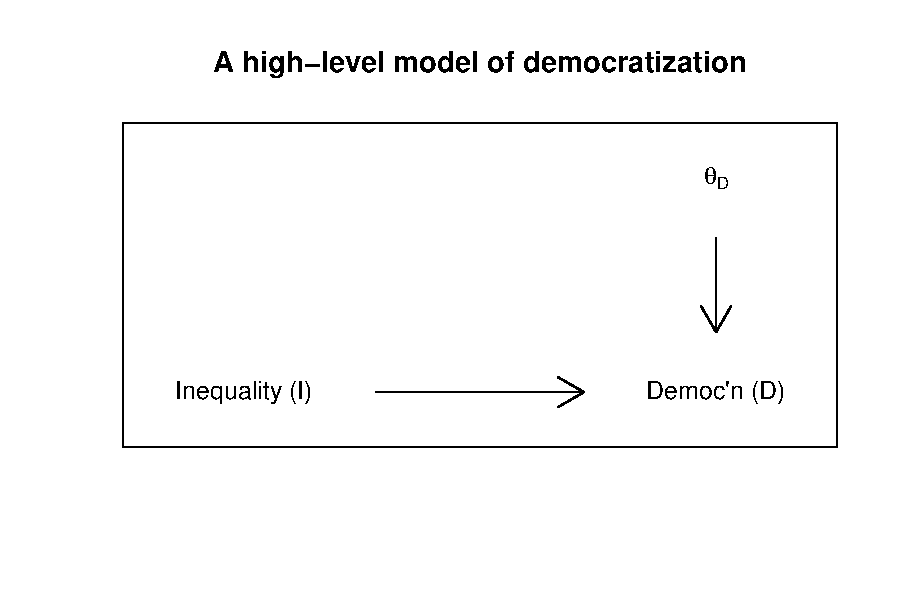
\includegraphics{ii_files/figure-latex/dagdemochigh-1} 

}

\caption{Simple democracy, inequality model}\label{fig:dagdemochigh}
\end{figure}

Nonetheless, we can increase the prospects for learning by \emph{theorizing} the relationship between inequality and democratization. Given causal logics and empirical findings in the existing literature, we can say more than is contained in Figure \ref{fig:dagdemochigh} about the possible structure of the causal linkages between inequality and democratization. And we can embed this prior knowledge of the possible causal relations in this domain in a lower-level model that is consistent with the high-level model that most simply represents our query. If we were to seek to fully capture them, the models developed by Boix, Acemoglu and Robinson, and Ansell and Samuels would, each individually, suggest causal graphs with a large number of nodes and edges connecting them. Representing all variables and relationships jointly contained in these three models would take an extremely complex graph. Yet there is no need to go down to the lowest possible level---to generate the \emph{most} detailed graph---in order to increase our empirical leverage on the problem.

We represent in Figure \ref{fig:lowdem} one possible lower-level model consistent with our high-level model. Drawing on causal logics in the existing literature, we unpack the nodes in the high-level model in two ways:

\begin{enumerate}
\def\labelenumi{\arabic{enumi}.}
\item
  We interpose a mediator between inequality and democratization: mobilization (\(M\)) by economically disadvantaged groups expressing material grievances. \(M\) is a function of both \(I\) and of its own response-type variable, \(\theta^M\), which defines its response to \(I\). In inserting this mediator, we have extracted \(\theta^M\) from \(\theta^D\), pulling out that part of \(D\)'s response to \(I\) that depends on \(M\)'s response to \(I\).
\item
  We specify a second influence on democratization, international pressure (\(P\)). Like \(\theta^M\), \(P\) has also been extracted from \(\theta^D\); it represents that part of \(D\)'s response to \(I\) that is conditioned by international pressures.
\end{enumerate}

\begin{figure}

{\centering 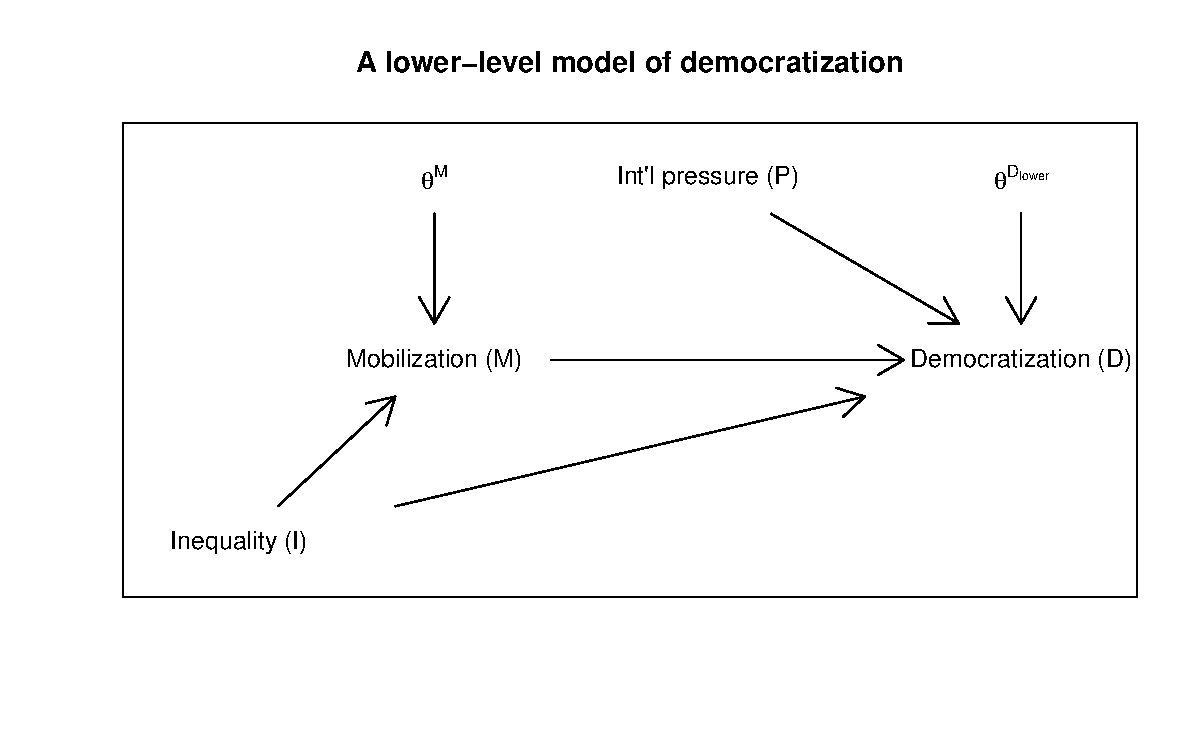
\includegraphics[width=.7\textwidth]{ii_files/figure-latex/unnamed-chunk-41-1} 

}

\caption{\label{fig:lowdem} A lower-level model of democratization in which inequality may affect regime type both directly and through mobilization of the lower classes, and international pressure may also affect regime type.}\label{fig:unnamed-chunk-41}
\end{figure}

In representing the causal dependencies in this graph, we allow for inequality to have (in the language of mediation analysis) both an ``indirect'' effect on democratization via mobilization and a ``direct'' effect. The arrow running directly from \(I\) to \(D\) allows for effects of inequality on democratization beyond any effects running via mobilization of the poor, including effects that might run in the opposite direction. (For instance, it is possible that inequality has a positive effect on democratization via mobilization but a negative effect via any number of processes that are not explicitly specified in the model.) The graph also implies that there is no confounding: since there is no arrow running from another variable in the graph to \(I\), \(I\) is assigned as-if randomly.

The lower-level graph thus has two exogenous, response-type nodes that will be relevant to assessing causal effects: \(\theta^M\) and \(\theta^{D_{lower}}\). \(\theta^M\), capturing \(I\)'s effect on \(M\), ranges across the usual four values for a single-cause, binary setup: \(\theta_{00}^M, \theta_{01}^M, \theta_{10}^M\), and \(\theta_{11}^M\).

\(\theta^{D_{lower}}\) is considerably more complicated, however, because this node represents \(D\)'s response to three causal variables: \(I\), \(M\), and \(P\). One way to put this is that the values of \(\theta^{D_{lower}}\) indicate how inequality's direct effect will depend on mobilization (and vice versa), conditional on whether or not there is international pressure. We need more complex notation than that introduced in Chapter 5 in order to represent the possible response types here. In Chapter 5, we used \(\theta_{ij}^{gh}\) to represent the potential outcomes for the four combinations of values that two binary variables can take on. With a third binary variable, we now use left as well as right super- and subscripts, as in: \(_{ij}^{gh}\theta_{mn}^{kl}\). In the current application, we let the left scripts represent the values that \(D\) will take on for different values of \(I\) and \(M\) \emph{when P=0} while the right scripts represent \(D\)'s potential outcomes for different values of \(I\) and \(M\) \emph{when P=1}. For each set of four scripts (left or right), moving horizontally from left to right represents a move from \(I=0\) to \(I=1\), while moving vertically from bottom to top represents a move from \(M=0\) to \(M=1\). (In other words, we can think of there being a separate \(I\)-by-\(M\) graph on either side of \(t\), one for \(P=0\) and one for \(P=1\), each with the origin in the lower lefthand corner.)

Thus, to illustrate, \(n\) represents the value that \(D\) will take on when \(I=1, M=0\), and \(P=1\), while \(j\) represents the outcome for those same values of \(I\) and \(M\) but when \(P=0\). Filling in numbers, \(_{01}^{01}\theta_{10}^{10}\) represents a type in which inequality always (regardless of mobilization) has a positive direct effect on democratization when \(P=0\) and always has a negative direct effect on democratization when \(P=1\); in which mobilization itself never has an effect; and in which international pressure has a positive effect when inequality is low but a negative effect when inequality is high.

The result is \(2^8=256\) possible response types for \(D\). With 4 response types for \(M\), we thus have 1024 possible combinations of causal effects between named variables in the lower-level graph. How do these lower-level response types map onto the higher-level response types that are of interest? In other words, which combinations of lower-level types represent a positive, negative, or zero causal effect of inequality on democratization?

To define a causal effect of \(I\) in this setup, we need to define the ``joint effect'' of two variables as being the effect of changing both variables simultaneously (in the same direction, unless otherwise specified). Thus, the joint effect of \(I\) and \(M\) on \(D\) is positive if changing both \(I\) and \(M\) from \(0\) to \(1\) changes \(D\) from \(0\) to \(1\). We can likewise refer to the joint effect of an increase in one variable and a decrease in another. Given this definition, a positive causal effect of inequality on democratization emerges for any of the following three sets of lower-level response patterns:

\begin{enumerate}
\def\labelenumi{\arabic{enumi}.}
\item
  \textbf{Linked positive mediated effects.} \(I\) has a positive effect on \(M\); and \(I\) and \(M\) have a \emph{joint} positive effect on \(D\) when \(P\) takes on whatever value it takes on in the case. Formally, this condition is satisfied when \(\theta^M=\theta^M_{01}\) and \(\theta^D_{lower}\) takes on any value consistent with \(_{0j}^{g1}\theta_{mn}^{kl}\) if \(P=0\) or with \(_{ij}^{gh}\theta_{0n}^{k1}\) if \(P=1\).
\item
  \textbf{Linked negative mediated effects} \(I\) has a negative effect on \(M\); and \(I\) and \(M\) have a \emph{joint} negative effect on \(D\) when \(P\) takes on whatever value it takes on in the case. This condition is satisfied when \(\theta^M=\theta^M_{10}\) and \(\theta^D_{lower}\) takes on any value consistent with \(_{i1}^{0h}\theta_{mn}^{kl}\) if \(P=0\) or with \(_{ij}^{gh}\theta_{m1}^{0l}\) if \(P=1\).
\item
  \textbf{Positive direct effect} \(I\) has no effect on \(M\) and \(I\) has a positive effect on \(D\) at whatever value \(M\) is fixed at and whatever value \(P\) takes on in the case. This condition is satisfied when \(\theta^M=\theta^M_{00}\) and \(\theta^D_{lower}\) takes on any value consistent with \(_{01}^{gh}\theta_{mn}^{kl}\) if \(P=0\) or with \(_{ij}^{gh}\theta_{01}^{kl}\) if \(P=1\); or when \(\theta^M=\theta^M_{11}\) and \(\theta^D_{lower}\) takes on any value consistent with \(_{ij}^{01}\theta_{mn}^{kl}\) if \(P=0\) or with \(_{ij}^{gh}\theta_{mn}^{01}\) if \(P=1\).
\end{enumerate}

If we start out with a case in which inequality is high and democratization has not occurred (or inequality is low and democratization \emph{has} occurred), we will be interested in the possibility of a negative causal effect. A negative causal effect of inequality on democratization emerges for any of the following three sets of lower-level response patterns:

\begin{enumerate}
\def\labelenumi{\arabic{enumi}.}
\setcounter{enumi}{3}
\item
  \textbf{Positive, then negative mediated effects} \(I\) has a positive effect on \(M\); and \(I\) and \(M\) have a \emph{joint} negative effect on \(D\) when \(P\) takes on whatever value it takes on in the case. This condition is satisfied when \(\theta^M=\theta^M_{01}\) and \(\theta^D_{lower}\) takes on any value consistent with \(_{1j}^{g0}\theta_{mn}^{kl}\) if \(P=0\) or with \(_{ij}^{gh}\theta_{1n}^{k0}\) if \(P=1\).
\item
  \textbf{Negative, then joint negative mediated effects} \(I\) has a negative effect on \(M\); and jointly increasing \(I\) while decreasing \(M\) generates a decrease in \(D\) when \(P\) takes on whatever value it takes on in the case. This condition is satisfied when \(\theta^M=\theta^M_{10}\) and \(\theta^D_{lower}\) takes on any value consistent with \(_{i0}^{1h}\theta_{mn}^{kl}\) if \(P=0\) or with \(_{ij}^{gh}\theta_{m0}^{1l}\) if \(P=1\).
\item
  \textbf{Negative direct effects} \(I\) has no effect on \(M\) and \(I\) has a negative effect on \(D\) at whatever value \(M\) is fixed at and whatever value \(P\) takes on in the case. This condition is satisfied when \(\theta^M=\theta^M_{00}\) and \(\theta^D_{lower}\) takes on any value consistent with \(_{10}^{gh}\theta_{mn}^{kl}\) if \(P=0\) or with \(_{ij}^{gh}\theta_{10}^{kl}\) if \(P=1\); or when \(\theta^M=\theta^M_{11}\) and \(\theta^D_{lower}\) takes on any value consistent with \(_{ij}^{10}\theta_{mn}^{kl}\) if \(P=0\) or with \(_{ij}^{gh}\theta_{mn}^{10}\) if \(P=1\).
\end{enumerate}

Finally, all other response patterns yield \emph{no} effect of inequality on democratization.

Thus, for a case in which \(I=D=1\), our query amounts to assessing the probability that \(\theta^M\) and \(\theta^D_{lower}\) jointly take on values falling into conditions 1, 2, or 3. And for a case in which \(I \neq D\), where we entertain the possibility of a negative effect, our query is an assessment of the probability of conditions 4, 5, and 6.

\hypertarget{forming-priors}{%
\subsection{Forming Priors}\label{forming-priors}}

We now need to express prior beliefs about the probability distribution from which values of \(\theta^M\) and \(\theta^D_{lower}\) are drawn. We place structure on this problem by drawing a set of beliefs about the likelihood or monotonicity of effects and interactions among variables from the theories in Boix, Acemoglu and Robinson, and Ansell and Samuels. As a heuristic device, we weight more heavily those propositions that are more widely shared across the three works than those that are consistent with only one of the frameworks. We intend this part of the exercise to be merely illustrative of how one might go about forming priors from an existing base of knowledge; there are undoubtedly other ways in which one could do so from the inequality and democracy literature.

Specifically, the belief that we embed in our priors about \(\theta^M\) is:

\begin{itemize}
\tightlist
\item
  \textbf{Monotonicity of \(I\)'s effect on \(M\)}: In Acemoglu and Robinson, inequality should generally increase the chances of---and, in Boix, should never prevent---mobilization by the poor. Only in Ansell and Samuels' model does inequality have a partial downward effect on the poor's demand for democracy insofar as improved material welfare for the poor increases the chances of autocratic expropriation; and this effect is countervailed by the greater redistributive gains that the poor will enjoy under democracy as inequality rises.\footnote{In addition, as the industrial bourgeoisie become richer, which increases the Gini, this group faces a greater risk of autocratic expropriation. If we consider the rising bourgeosie's mobilization to be mobilization by a materially disadvantaged group, then this constitutes an additional positive effect of inequality on mobilization.} Consistent with the weight of prior theory on this effect, in our initial run of the analysis, we rule out negative effects of \(I\) on \(M\). We are indifferent in our priors between positive and null effects and between the two types of null effects (mobilization always occurring or never occurring, regardless of the level of inequality). We thus set our prior on \(\theta^M\) as: \(p(\theta^M=\theta^M_{10})=0.0\), \(p(\theta^M=\theta^M_{00})=0.25\), \(p(\theta^M=\theta^M_{11})=0.25\), and \(p(\theta^M=\theta^M_{01})=0.5\). We relax this monotonicity assumption, to account for the Ansell and Samuels logic, in a second run of the analysis.
\end{itemize}

For our prior on democracy's responses to inequality, mobilization, and international pressure (\(\theta^D_{lower}\)), we extract the following beliefs from the literature:

\begin{itemize}
\item
  \textbf{Monotonicity of direct \(I\) effect: no positive effect}: In none of the three theories does inequality promote democratization via a pathway \emph{other than} via the poor's rising demand for it. In all three theories, inequality has a distinct negative effect on democratization via an increase in the elite's expected losses under democracy and thus its willingness to repress. In Ansell and Samuels, the distribution of resources also affects the probability of success of rebellion; thus higher inequality also reduces the prospects for democratization by strengthening the elite's hold on power. We thus set a zero prior probability on all types in which \(I\)'s direct effect on \(D\) is positive for any value of \(P\). This excludes all of the families of type \(_{01}^{xx}\theta_{xx}^{xx}\), \(_{xx}^{01}\theta_{xx}^{xx}\), \(_{xx}^{xx}\theta_{01}^{xx}\), and \(_{xx}^{xx}\theta_{xx}^{01}\). Apologies for dense notation.
\item
  \textbf{Monotonicity of \(M\)'s effect: no negative effect}: In none of the three theories does mobilization reduce the prospects of democratization. We thus set a zero probability on all types in which \(M\)'s effect on \(D\) is negative at any value of \(I\) or \(P\). This excludes all of the families of type \(_{1x}^{0x}\theta_{xx}^{xx}\), \(_{x1}^{x0}\theta_{xx}^{xx}\), \(_{xx}^{xx}\theta_{1x}^{0x}\), and \(_{xx}^{xx}\theta_{x1}^{x0}\).
\item
  \textbf{Monotonicity of \(P\)'s effect: no negative effect}: While international pressures are only discussed in Haggard and Kaufman's study, none of the studies considers the possibility that international pressures to democratize might prevent democratization that would otherwise have occurred. We thus set a zero probability on all types in which \(P\)'s effect is negative at any value of \(I\) or \(M\). This excludes all of the families of type \(_{1x}^{xx}\theta_{0x}^{xx}\), \(_{x1}^{xx}\theta_{x0}^{xx}\), \(_{xx}^{1x}\theta_{xx}^{0x}\), and \(_{xx}^{x1}\theta_{xx}^{x0}\).
\end{itemize}

For all remaining, allowable types, we set flat priors.

We summarize the set of excluded types in Table \ref{tab:apptypes}. To ease interpretation of types, we also indicate, for all excluded types, the reason for the exclusion.

\begin{longtable}[]{@{}ccccc@{}}
\caption{\label{tab:apptypes} Possible (families of) types defining the possible effects of inequality (\(I\)), mobilization, (\(M\)), and international pressure (\(P\)) on democratization. We exclude families based on a set of monotonicity assumptions, which reduces the allowable types from 256 to 20.}\tabularnewline
\toprule
\begin{minipage}[b]{0.24\columnwidth}\centering
Family or Type\strut
\end{minipage} & \begin{minipage}[b]{0.09\columnwidth}\centering
Excluded?\strut
\end{minipage} & \begin{minipage}[b]{0.20\columnwidth}\centering
Reason for Exclusion\strut
\end{minipage} & \begin{minipage}[b]{0.18\columnwidth}\centering
Nature of interaction\strut
\end{minipage} & \begin{minipage}[b]{0.15\columnwidth}\centering
Prior probability\strut
\end{minipage}\tabularnewline
\midrule
\endfirsthead
\toprule
\begin{minipage}[b]{0.24\columnwidth}\centering
Family or Type\strut
\end{minipage} & \begin{minipage}[b]{0.09\columnwidth}\centering
Excluded?\strut
\end{minipage} & \begin{minipage}[b]{0.20\columnwidth}\centering
Reason for Exclusion\strut
\end{minipage} & \begin{minipage}[b]{0.18\columnwidth}\centering
Nature of interaction\strut
\end{minipage} & \begin{minipage}[b]{0.15\columnwidth}\centering
Prior probability\strut
\end{minipage}\tabularnewline
\midrule
\endhead
\begin{minipage}[t]{0.24\columnwidth}\centering
\(_{01}^{xx}\theta_{xx}^{xx}\)\strut
\end{minipage} & \begin{minipage}[t]{0.09\columnwidth}\centering
Yes\strut
\end{minipage} & \begin{minipage}[t]{0.20\columnwidth}\centering
No + \(I\) effects\strut
\end{minipage} & \begin{minipage}[t]{0.18\columnwidth}\centering
\strut
\end{minipage} & \begin{minipage}[t]{0.15\columnwidth}\centering
0\strut
\end{minipage}\tabularnewline
\begin{minipage}[t]{0.24\columnwidth}\centering
\strut
\end{minipage} & \begin{minipage}[t]{0.09\columnwidth}\centering
\strut
\end{minipage} & \begin{minipage}[t]{0.20\columnwidth}\centering
\strut
\end{minipage} & \begin{minipage}[t]{0.18\columnwidth}\centering
\strut
\end{minipage} & \begin{minipage}[t]{0.15\columnwidth}\centering
\strut
\end{minipage}\tabularnewline
\begin{minipage}[t]{0.24\columnwidth}\centering
\(_{xx}^{01}\theta_{xx}^{xx}\)\strut
\end{minipage} & \begin{minipage}[t]{0.09\columnwidth}\centering
Yes\strut
\end{minipage} & \begin{minipage}[t]{0.20\columnwidth}\centering
No + \(I\) effects\strut
\end{minipage} & \begin{minipage}[t]{0.18\columnwidth}\centering
\strut
\end{minipage} & \begin{minipage}[t]{0.15\columnwidth}\centering
0\strut
\end{minipage}\tabularnewline
\begin{minipage}[t]{0.24\columnwidth}\centering
\strut
\end{minipage} & \begin{minipage}[t]{0.09\columnwidth}\centering
\strut
\end{minipage} & \begin{minipage}[t]{0.20\columnwidth}\centering
\strut
\end{minipage} & \begin{minipage}[t]{0.18\columnwidth}\centering
\strut
\end{minipage} & \begin{minipage}[t]{0.15\columnwidth}\centering
\strut
\end{minipage}\tabularnewline
\begin{minipage}[t]{0.24\columnwidth}\centering
\(_{xx}^{xx}\theta_{01}^{xx}\)\strut
\end{minipage} & \begin{minipage}[t]{0.09\columnwidth}\centering
Yes\strut
\end{minipage} & \begin{minipage}[t]{0.20\columnwidth}\centering
No + \(I\) effects\strut
\end{minipage} & \begin{minipage}[t]{0.18\columnwidth}\centering
\strut
\end{minipage} & \begin{minipage}[t]{0.15\columnwidth}\centering
0\strut
\end{minipage}\tabularnewline
\begin{minipage}[t]{0.24\columnwidth}\centering
\strut
\end{minipage} & \begin{minipage}[t]{0.09\columnwidth}\centering
\strut
\end{minipage} & \begin{minipage}[t]{0.20\columnwidth}\centering
\strut
\end{minipage} & \begin{minipage}[t]{0.18\columnwidth}\centering
\strut
\end{minipage} & \begin{minipage}[t]{0.15\columnwidth}\centering
\strut
\end{minipage}\tabularnewline
\begin{minipage}[t]{0.24\columnwidth}\centering
\(_{xx}^{xx}\theta_{xx}^{01}\)\strut
\end{minipage} & \begin{minipage}[t]{0.09\columnwidth}\centering
Yes\strut
\end{minipage} & \begin{minipage}[t]{0.20\columnwidth}\centering
No + \(I\) effects\strut
\end{minipage} & \begin{minipage}[t]{0.18\columnwidth}\centering
\strut
\end{minipage} & \begin{minipage}[t]{0.15\columnwidth}\centering
0\strut
\end{minipage}\tabularnewline
\begin{minipage}[t]{0.24\columnwidth}\centering
\strut
\end{minipage} & \begin{minipage}[t]{0.09\columnwidth}\centering
\strut
\end{minipage} & \begin{minipage}[t]{0.20\columnwidth}\centering
\strut
\end{minipage} & \begin{minipage}[t]{0.18\columnwidth}\centering
\strut
\end{minipage} & \begin{minipage}[t]{0.15\columnwidth}\centering
\strut
\end{minipage}\tabularnewline
\begin{minipage}[t]{0.24\columnwidth}\centering
\(_{1x}^{0x}\theta_{xx}^{xx}\)\strut
\end{minipage} & \begin{minipage}[t]{0.09\columnwidth}\centering
Yes\strut
\end{minipage} & \begin{minipage}[t]{0.20\columnwidth}\centering
No - \(M\) effects\strut
\end{minipage} & \begin{minipage}[t]{0.18\columnwidth}\centering
\strut
\end{minipage} & \begin{minipage}[t]{0.15\columnwidth}\centering
0\strut
\end{minipage}\tabularnewline
\begin{minipage}[t]{0.24\columnwidth}\centering
\strut
\end{minipage} & \begin{minipage}[t]{0.09\columnwidth}\centering
\strut
\end{minipage} & \begin{minipage}[t]{0.20\columnwidth}\centering
\strut
\end{minipage} & \begin{minipage}[t]{0.18\columnwidth}\centering
\strut
\end{minipage} & \begin{minipage}[t]{0.15\columnwidth}\centering
\strut
\end{minipage}\tabularnewline
\begin{minipage}[t]{0.24\columnwidth}\centering
\(_{x1}^{x0}\theta_{xx}^{xx}\)\strut
\end{minipage} & \begin{minipage}[t]{0.09\columnwidth}\centering
Yes\strut
\end{minipage} & \begin{minipage}[t]{0.20\columnwidth}\centering
No - \(M\) effects\strut
\end{minipage} & \begin{minipage}[t]{0.18\columnwidth}\centering
\strut
\end{minipage} & \begin{minipage}[t]{0.15\columnwidth}\centering
0\strut
\end{minipage}\tabularnewline
\begin{minipage}[t]{0.24\columnwidth}\centering
\strut
\end{minipage} & \begin{minipage}[t]{0.09\columnwidth}\centering
\strut
\end{minipage} & \begin{minipage}[t]{0.20\columnwidth}\centering
\strut
\end{minipage} & \begin{minipage}[t]{0.18\columnwidth}\centering
\strut
\end{minipage} & \begin{minipage}[t]{0.15\columnwidth}\centering
\strut
\end{minipage}\tabularnewline
\begin{minipage}[t]{0.24\columnwidth}\centering
\(_{xx}^{xx}\theta_{1x}^{0x}\)\strut
\end{minipage} & \begin{minipage}[t]{0.09\columnwidth}\centering
Yes\strut
\end{minipage} & \begin{minipage}[t]{0.20\columnwidth}\centering
No - \(M\) effects\strut
\end{minipage} & \begin{minipage}[t]{0.18\columnwidth}\centering
\strut
\end{minipage} & \begin{minipage}[t]{0.15\columnwidth}\centering
0\strut
\end{minipage}\tabularnewline
\begin{minipage}[t]{0.24\columnwidth}\centering
\strut
\end{minipage} & \begin{minipage}[t]{0.09\columnwidth}\centering
\strut
\end{minipage} & \begin{minipage}[t]{0.20\columnwidth}\centering
\strut
\end{minipage} & \begin{minipage}[t]{0.18\columnwidth}\centering
\strut
\end{minipage} & \begin{minipage}[t]{0.15\columnwidth}\centering
\strut
\end{minipage}\tabularnewline
\begin{minipage}[t]{0.24\columnwidth}\centering
\(_{xx}^{xx}\theta_{x1}^{x0}\)\strut
\end{minipage} & \begin{minipage}[t]{0.09\columnwidth}\centering
Yes\strut
\end{minipage} & \begin{minipage}[t]{0.20\columnwidth}\centering
No - \(M\) effects\strut
\end{minipage} & \begin{minipage}[t]{0.18\columnwidth}\centering
\strut
\end{minipage} & \begin{minipage}[t]{0.15\columnwidth}\centering
0\strut
\end{minipage}\tabularnewline
\begin{minipage}[t]{0.24\columnwidth}\centering
\strut
\end{minipage} & \begin{minipage}[t]{0.09\columnwidth}\centering
\strut
\end{minipage} & \begin{minipage}[t]{0.20\columnwidth}\centering
\strut
\end{minipage} & \begin{minipage}[t]{0.18\columnwidth}\centering
\strut
\end{minipage} & \begin{minipage}[t]{0.15\columnwidth}\centering
\strut
\end{minipage}\tabularnewline
\begin{minipage}[t]{0.24\columnwidth}\centering
\(_{1x}^{xx}\theta_{0x}^{xx}\)\strut
\end{minipage} & \begin{minipage}[t]{0.09\columnwidth}\centering
Yes\strut
\end{minipage} & \begin{minipage}[t]{0.20\columnwidth}\centering
No - \(P\) effects\strut
\end{minipage} & \begin{minipage}[t]{0.18\columnwidth}\centering
\strut
\end{minipage} & \begin{minipage}[t]{0.15\columnwidth}\centering
0\strut
\end{minipage}\tabularnewline
\begin{minipage}[t]{0.24\columnwidth}\centering
\strut
\end{minipage} & \begin{minipage}[t]{0.09\columnwidth}\centering
\strut
\end{minipage} & \begin{minipage}[t]{0.20\columnwidth}\centering
\strut
\end{minipage} & \begin{minipage}[t]{0.18\columnwidth}\centering
\strut
\end{minipage} & \begin{minipage}[t]{0.15\columnwidth}\centering
\strut
\end{minipage}\tabularnewline
\begin{minipage}[t]{0.24\columnwidth}\centering
\(_{x1}^{xx}\theta_{x0}^{xx}\)\strut
\end{minipage} & \begin{minipage}[t]{0.09\columnwidth}\centering
Yes\strut
\end{minipage} & \begin{minipage}[t]{0.20\columnwidth}\centering
No - \(P\) effects\strut
\end{minipage} & \begin{minipage}[t]{0.18\columnwidth}\centering
\strut
\end{minipage} & \begin{minipage}[t]{0.15\columnwidth}\centering
0\strut
\end{minipage}\tabularnewline
\begin{minipage}[t]{0.24\columnwidth}\centering
\strut
\end{minipage} & \begin{minipage}[t]{0.09\columnwidth}\centering
\strut
\end{minipage} & \begin{minipage}[t]{0.20\columnwidth}\centering
\strut
\end{minipage} & \begin{minipage}[t]{0.18\columnwidth}\centering
\strut
\end{minipage} & \begin{minipage}[t]{0.15\columnwidth}\centering
\strut
\end{minipage}\tabularnewline
\begin{minipage}[t]{0.24\columnwidth}\centering
\(_{xx}^{1x}\theta_{xx}^{0x}\)\strut
\end{minipage} & \begin{minipage}[t]{0.09\columnwidth}\centering
Yes\strut
\end{minipage} & \begin{minipage}[t]{0.20\columnwidth}\centering
No - \(P\) effects\strut
\end{minipage} & \begin{minipage}[t]{0.18\columnwidth}\centering
\strut
\end{minipage} & \begin{minipage}[t]{0.15\columnwidth}\centering
0\strut
\end{minipage}\tabularnewline
\begin{minipage}[t]{0.24\columnwidth}\centering
\strut
\end{minipage} & \begin{minipage}[t]{0.09\columnwidth}\centering
\strut
\end{minipage} & \begin{minipage}[t]{0.20\columnwidth}\centering
\strut
\end{minipage} & \begin{minipage}[t]{0.18\columnwidth}\centering
\strut
\end{minipage} & \begin{minipage}[t]{0.15\columnwidth}\centering
\strut
\end{minipage}\tabularnewline
\begin{minipage}[t]{0.24\columnwidth}\centering
\(_{xx}^{x1}\theta_{xx}^{x0}\)\strut
\end{minipage} & \begin{minipage}[t]{0.09\columnwidth}\centering
Yes\strut
\end{minipage} & \begin{minipage}[t]{0.20\columnwidth}\centering
No - \(P\) effects\strut
\end{minipage} & \begin{minipage}[t]{0.18\columnwidth}\centering
\strut
\end{minipage} & \begin{minipage}[t]{0.15\columnwidth}\centering
0\strut
\end{minipage}\tabularnewline
\begin{minipage}[t]{0.24\columnwidth}\centering
\strut
\end{minipage} & \begin{minipage}[t]{0.09\columnwidth}\centering
\strut
\end{minipage} & \begin{minipage}[t]{0.20\columnwidth}\centering
\strut
\end{minipage} & \begin{minipage}[t]{0.18\columnwidth}\centering
\strut
\end{minipage} & \begin{minipage}[t]{0.15\columnwidth}\centering
\strut
\end{minipage}\tabularnewline
\bottomrule
\end{longtable}

In Table \ref{tab:apptypes2} we show, for the remainig 20 allowable types, how international pressure moderates the effects of inequality (direct) and mobilization. We use the following notation to characterize conditioning effects of pressure on the effect of another variable, \(X\):

\begin{itemize}
\item
  \(N\): \(P\) has no moderating effect
\item
  \(O_X\): \(P=1\) creates an ``opportunity'' for \(X\) to have an effect that it does not have at \(P=0\); at \(P=1\) and \(X=0\), \(D\) takes on the value it does when \(X=0\) and \(X\) has an effect, but does not take on this value when \(P=0\) and \(X=0\)
\item
  \(C_X\): \(P=1\) is a causal ``complement'' to \(X\), allowing \(X\) to have an effect it did not have at \(P=0\); at \(P=1\) and \(X=1\), \(D\) takes on the value it does when \(X=1\) and \(X\) has an effect, but does not take on this value when \(P=0\) and \(X=1\)
\item
  \(S_X\): \(P=1\) ``substitutes'' for \(X\), generating the outcome that \(X=1\) was necessary to generate at \(P=0\); at \(P=1\) and \(X=0\), \(D\) takes on the value it does when \(X=1\) and \(X\) has an effect, but does not take on this value when \(P=0\) and \(X=0\)
\item
  \(E_X\): \(P\) ``eliminates'' \(X\)'s effect, preventing \(X=1\) from generating the outcome it generates when \(P=0\); at \(P=1\) and \(X=1\), \(D\) does not take on the value it does when \(X=1\) and \(X\) has an effect, but does take on this value when \(P=0\) and \(X=1\)
\end{itemize}

\begin{longtable}[]{@{}ccccc@{}}
\caption{\label{tab:apptypes2} Table of allowable types. The table characterizes the nature of the interaction, using the notation explained in the main text. We impose flat priors across all non-excluded types.}\tabularnewline
\toprule
\begin{minipage}[b]{0.24\columnwidth}\centering
Family or Type\strut
\end{minipage} & \begin{minipage}[b]{0.09\columnwidth}\centering
Excluded?\strut
\end{minipage} & \begin{minipage}[b]{0.20\columnwidth}\centering
Reason for Exclusion\strut
\end{minipage} & \begin{minipage}[b]{0.18\columnwidth}\centering
Nature of interaction\strut
\end{minipage} & \begin{minipage}[b]{0.15\columnwidth}\centering
Prior probability\strut
\end{minipage}\tabularnewline
\midrule
\endfirsthead
\toprule
\begin{minipage}[b]{0.24\columnwidth}\centering
Family or Type\strut
\end{minipage} & \begin{minipage}[b]{0.09\columnwidth}\centering
Excluded?\strut
\end{minipage} & \begin{minipage}[b]{0.20\columnwidth}\centering
Reason for Exclusion\strut
\end{minipage} & \begin{minipage}[b]{0.18\columnwidth}\centering
Nature of interaction\strut
\end{minipage} & \begin{minipage}[b]{0.15\columnwidth}\centering
Prior probability\strut
\end{minipage}\tabularnewline
\midrule
\endhead
\begin{minipage}[t]{0.24\columnwidth}\centering
\(_{00}^{00}\theta_{00}^{00}\)\strut
\end{minipage} & \begin{minipage}[t]{0.09\columnwidth}\centering
\strut
\end{minipage} & \begin{minipage}[t]{0.20\columnwidth}\centering
\strut
\end{minipage} & \begin{minipage}[t]{0.18\columnwidth}\centering
\(N\)\strut
\end{minipage} & \begin{minipage}[t]{0.15\columnwidth}\centering
0.05\strut
\end{minipage}\tabularnewline
\begin{minipage}[t]{0.24\columnwidth}\centering
\strut
\end{minipage} & \begin{minipage}[t]{0.09\columnwidth}\centering
\strut
\end{minipage} & \begin{minipage}[t]{0.20\columnwidth}\centering
\strut
\end{minipage} & \begin{minipage}[t]{0.18\columnwidth}\centering
\strut
\end{minipage} & \begin{minipage}[t]{0.15\columnwidth}\centering
\strut
\end{minipage}\tabularnewline
\begin{minipage}[t]{0.24\columnwidth}\centering
\(_{00}^{00}\theta_{00}^{10}\)\strut
\end{minipage} & \begin{minipage}[t]{0.09\columnwidth}\centering
\strut
\end{minipage} & \begin{minipage}[t]{0.20\columnwidth}\centering
\strut
\end{minipage} & \begin{minipage}[t]{0.18\columnwidth}\centering
\(C_M, O_I\)\strut
\end{minipage} & \begin{minipage}[t]{0.15\columnwidth}\centering
0.05\strut
\end{minipage}\tabularnewline
\begin{minipage}[t]{0.24\columnwidth}\centering
\strut
\end{minipage} & \begin{minipage}[t]{0.09\columnwidth}\centering
\strut
\end{minipage} & \begin{minipage}[t]{0.20\columnwidth}\centering
\strut
\end{minipage} & \begin{minipage}[t]{0.18\columnwidth}\centering
\strut
\end{minipage} & \begin{minipage}[t]{0.15\columnwidth}\centering
\strut
\end{minipage}\tabularnewline
\begin{minipage}[t]{0.24\columnwidth}\centering
\(_{00}^{00}\theta_{00}^{11}\)\strut
\end{minipage} & \begin{minipage}[t]{0.09\columnwidth}\centering
\strut
\end{minipage} & \begin{minipage}[t]{0.20\columnwidth}\centering
\strut
\end{minipage} & \begin{minipage}[t]{0.18\columnwidth}\centering
\(C_M\)\strut
\end{minipage} & \begin{minipage}[t]{0.15\columnwidth}\centering
0.05\strut
\end{minipage}\tabularnewline
\begin{minipage}[t]{0.24\columnwidth}\centering
\strut
\end{minipage} & \begin{minipage}[t]{0.09\columnwidth}\centering
\strut
\end{minipage} & \begin{minipage}[t]{0.20\columnwidth}\centering
\strut
\end{minipage} & \begin{minipage}[t]{0.18\columnwidth}\centering
\strut
\end{minipage} & \begin{minipage}[t]{0.15\columnwidth}\centering
\strut
\end{minipage}\tabularnewline
\begin{minipage}[t]{0.24\columnwidth}\centering
\(_{00}^{00}\theta_{10}^{10}\)\strut
\end{minipage} & \begin{minipage}[t]{0.09\columnwidth}\centering
\strut
\end{minipage} & \begin{minipage}[t]{0.20\columnwidth}\centering
\strut
\end{minipage} & \begin{minipage}[t]{0.18\columnwidth}\centering
\(O_I\)\strut
\end{minipage} & \begin{minipage}[t]{0.15\columnwidth}\centering
0.05\strut
\end{minipage}\tabularnewline
\begin{minipage}[t]{0.24\columnwidth}\centering
\strut
\end{minipage} & \begin{minipage}[t]{0.09\columnwidth}\centering
\strut
\end{minipage} & \begin{minipage}[t]{0.20\columnwidth}\centering
\strut
\end{minipage} & \begin{minipage}[t]{0.18\columnwidth}\centering
\strut
\end{minipage} & \begin{minipage}[t]{0.15\columnwidth}\centering
\strut
\end{minipage}\tabularnewline
\begin{minipage}[t]{0.24\columnwidth}\centering
\(_{00}^{00}\theta_{10}^{11}\)\strut
\end{minipage} & \begin{minipage}[t]{0.09\columnwidth}\centering
\strut
\end{minipage} & \begin{minipage}[t]{0.20\columnwidth}\centering
\strut
\end{minipage} & \begin{minipage}[t]{0.18\columnwidth}\centering
\(C_M, S_M, O_I\)\strut
\end{minipage} & \begin{minipage}[t]{0.15\columnwidth}\centering
0.05\strut
\end{minipage}\tabularnewline
\begin{minipage}[t]{0.24\columnwidth}\centering
\strut
\end{minipage} & \begin{minipage}[t]{0.09\columnwidth}\centering
\strut
\end{minipage} & \begin{minipage}[t]{0.20\columnwidth}\centering
\strut
\end{minipage} & \begin{minipage}[t]{0.18\columnwidth}\centering
\strut
\end{minipage} & \begin{minipage}[t]{0.15\columnwidth}\centering
\strut
\end{minipage}\tabularnewline
\begin{minipage}[t]{0.24\columnwidth}\centering
\(_{00}^{00}\theta_{11}^{11}\)\strut
\end{minipage} & \begin{minipage}[t]{0.09\columnwidth}\centering
\strut
\end{minipage} & \begin{minipage}[t]{0.20\columnwidth}\centering
\strut
\end{minipage} & \begin{minipage}[t]{0.18\columnwidth}\centering
\(N\)\strut
\end{minipage} & \begin{minipage}[t]{0.15\columnwidth}\centering
0.05\strut
\end{minipage}\tabularnewline
\begin{minipage}[t]{0.24\columnwidth}\centering
\strut
\end{minipage} & \begin{minipage}[t]{0.09\columnwidth}\centering
\strut
\end{minipage} & \begin{minipage}[t]{0.20\columnwidth}\centering
\strut
\end{minipage} & \begin{minipage}[t]{0.18\columnwidth}\centering
\strut
\end{minipage} & \begin{minipage}[t]{0.15\columnwidth}\centering
\strut
\end{minipage}\tabularnewline
\begin{minipage}[t]{0.24\columnwidth}\centering
\(_{00}^{10}\theta_{00}^{10}\)\strut
\end{minipage} & \begin{minipage}[t]{0.09\columnwidth}\centering
\strut
\end{minipage} & \begin{minipage}[t]{0.20\columnwidth}\centering
\strut
\end{minipage} & \begin{minipage}[t]{0.18\columnwidth}\centering
\(N\)\strut
\end{minipage} & \begin{minipage}[t]{0.15\columnwidth}\centering
0.05\strut
\end{minipage}\tabularnewline
\begin{minipage}[t]{0.24\columnwidth}\centering
\strut
\end{minipage} & \begin{minipage}[t]{0.09\columnwidth}\centering
\strut
\end{minipage} & \begin{minipage}[t]{0.20\columnwidth}\centering
\strut
\end{minipage} & \begin{minipage}[t]{0.18\columnwidth}\centering
\strut
\end{minipage} & \begin{minipage}[t]{0.15\columnwidth}\centering
\strut
\end{minipage}\tabularnewline
\begin{minipage}[t]{0.24\columnwidth}\centering
\(_{00}^{10}\theta_{00}^{11}\)\strut
\end{minipage} & \begin{minipage}[t]{0.09\columnwidth}\centering
\strut
\end{minipage} & \begin{minipage}[t]{0.20\columnwidth}\centering
\strut
\end{minipage} & \begin{minipage}[t]{0.18\columnwidth}\centering
\(C_M, E_I\)\strut
\end{minipage} & \begin{minipage}[t]{0.15\columnwidth}\centering
0.05\strut
\end{minipage}\tabularnewline
\begin{minipage}[t]{0.24\columnwidth}\centering
\strut
\end{minipage} & \begin{minipage}[t]{0.09\columnwidth}\centering
\strut
\end{minipage} & \begin{minipage}[t]{0.20\columnwidth}\centering
\strut
\end{minipage} & \begin{minipage}[t]{0.18\columnwidth}\centering
\strut
\end{minipage} & \begin{minipage}[t]{0.15\columnwidth}\centering
\strut
\end{minipage}\tabularnewline
\begin{minipage}[t]{0.24\columnwidth}\centering
\(_{00}^{10}\theta_{10}^{10}\)\strut
\end{minipage} & \begin{minipage}[t]{0.09\columnwidth}\centering
\strut
\end{minipage} & \begin{minipage}[t]{0.20\columnwidth}\centering
\strut
\end{minipage} & \begin{minipage}[t]{0.18\columnwidth}\centering
\(S_M, O_I\)\strut
\end{minipage} & \begin{minipage}[t]{0.15\columnwidth}\centering
0.05\strut
\end{minipage}\tabularnewline
\begin{minipage}[t]{0.24\columnwidth}\centering
\strut
\end{minipage} & \begin{minipage}[t]{0.09\columnwidth}\centering
\strut
\end{minipage} & \begin{minipage}[t]{0.20\columnwidth}\centering
\strut
\end{minipage} & \begin{minipage}[t]{0.18\columnwidth}\centering
\strut
\end{minipage} & \begin{minipage}[t]{0.15\columnwidth}\centering
\strut
\end{minipage}\tabularnewline
\begin{minipage}[t]{0.24\columnwidth}\centering
\(_{00}^{10}\theta_{10}^{11}\)\strut
\end{minipage} & \begin{minipage}[t]{0.09\columnwidth}\centering
\strut
\end{minipage} & \begin{minipage}[t]{0.20\columnwidth}\centering
\strut
\end{minipage} & \begin{minipage}[t]{0.18\columnwidth}\centering
\(S_M, E_I, O_I\)\strut
\end{minipage} & \begin{minipage}[t]{0.15\columnwidth}\centering
0.05\strut
\end{minipage}\tabularnewline
\begin{minipage}[t]{0.24\columnwidth}\centering
\strut
\end{minipage} & \begin{minipage}[t]{0.09\columnwidth}\centering
\strut
\end{minipage} & \begin{minipage}[t]{0.20\columnwidth}\centering
\strut
\end{minipage} & \begin{minipage}[t]{0.18\columnwidth}\centering
\strut
\end{minipage} & \begin{minipage}[t]{0.15\columnwidth}\centering
\strut
\end{minipage}\tabularnewline
\begin{minipage}[t]{0.24\columnwidth}\centering
\(_{00}^{10}\theta_{11}^{11}\)\strut
\end{minipage} & \begin{minipage}[t]{0.09\columnwidth}\centering
\strut
\end{minipage} & \begin{minipage}[t]{0.20\columnwidth}\centering
\strut
\end{minipage} & \begin{minipage}[t]{0.18\columnwidth}\centering
\(S_M, E_I\)\strut
\end{minipage} & \begin{minipage}[t]{0.15\columnwidth}\centering
0.05\strut
\end{minipage}\tabularnewline
\begin{minipage}[t]{0.24\columnwidth}\centering
\strut
\end{minipage} & \begin{minipage}[t]{0.09\columnwidth}\centering
\strut
\end{minipage} & \begin{minipage}[t]{0.20\columnwidth}\centering
\strut
\end{minipage} & \begin{minipage}[t]{0.18\columnwidth}\centering
\strut
\end{minipage} & \begin{minipage}[t]{0.15\columnwidth}\centering
\strut
\end{minipage}\tabularnewline
\begin{minipage}[t]{0.24\columnwidth}\centering
\(_{00}^{11}\theta_{00}^{11}\)\strut
\end{minipage} & \begin{minipage}[t]{0.09\columnwidth}\centering
\strut
\end{minipage} & \begin{minipage}[t]{0.20\columnwidth}\centering
\strut
\end{minipage} & \begin{minipage}[t]{0.18\columnwidth}\centering
\(N\)\strut
\end{minipage} & \begin{minipage}[t]{0.15\columnwidth}\centering
0.05\strut
\end{minipage}\tabularnewline
\begin{minipage}[t]{0.24\columnwidth}\centering
\strut
\end{minipage} & \begin{minipage}[t]{0.09\columnwidth}\centering
\strut
\end{minipage} & \begin{minipage}[t]{0.20\columnwidth}\centering
\strut
\end{minipage} & \begin{minipage}[t]{0.18\columnwidth}\centering
\strut
\end{minipage} & \begin{minipage}[t]{0.15\columnwidth}\centering
\strut
\end{minipage}\tabularnewline
\begin{minipage}[t]{0.24\columnwidth}\centering
\(_{00}^{11}\theta_{10}^{11}\)\strut
\end{minipage} & \begin{minipage}[t]{0.09\columnwidth}\centering
\strut
\end{minipage} & \begin{minipage}[t]{0.20\columnwidth}\centering
\strut
\end{minipage} & \begin{minipage}[t]{0.18\columnwidth}\centering
\(S_M, O_I\)\strut
\end{minipage} & \begin{minipage}[t]{0.15\columnwidth}\centering
0.05\strut
\end{minipage}\tabularnewline
\begin{minipage}[t]{0.24\columnwidth}\centering
\strut
\end{minipage} & \begin{minipage}[t]{0.09\columnwidth}\centering
\strut
\end{minipage} & \begin{minipage}[t]{0.20\columnwidth}\centering
\strut
\end{minipage} & \begin{minipage}[t]{0.18\columnwidth}\centering
\strut
\end{minipage} & \begin{minipage}[t]{0.15\columnwidth}\centering
\strut
\end{minipage}\tabularnewline
\begin{minipage}[t]{0.24\columnwidth}\centering
\(_{00}^{11}\theta_{11}^{11}\)\strut
\end{minipage} & \begin{minipage}[t]{0.09\columnwidth}\centering
\strut
\end{minipage} & \begin{minipage}[t]{0.20\columnwidth}\centering
\strut
\end{minipage} & \begin{minipage}[t]{0.18\columnwidth}\centering
\(S_M\)\strut
\end{minipage} & \begin{minipage}[t]{0.15\columnwidth}\centering
0.05\strut
\end{minipage}\tabularnewline
\begin{minipage}[t]{0.24\columnwidth}\centering
\strut
\end{minipage} & \begin{minipage}[t]{0.09\columnwidth}\centering
\strut
\end{minipage} & \begin{minipage}[t]{0.20\columnwidth}\centering
\strut
\end{minipage} & \begin{minipage}[t]{0.18\columnwidth}\centering
\strut
\end{minipage} & \begin{minipage}[t]{0.15\columnwidth}\centering
\strut
\end{minipage}\tabularnewline
\begin{minipage}[t]{0.24\columnwidth}\centering
\(_{10}^{10}\theta_{10}^{10}\)\strut
\end{minipage} & \begin{minipage}[t]{0.09\columnwidth}\centering
\strut
\end{minipage} & \begin{minipage}[t]{0.20\columnwidth}\centering
\strut
\end{minipage} & \begin{minipage}[t]{0.18\columnwidth}\centering
\(N\)\strut
\end{minipage} & \begin{minipage}[t]{0.15\columnwidth}\centering
0.05\strut
\end{minipage}\tabularnewline
\begin{minipage}[t]{0.24\columnwidth}\centering
\strut
\end{minipage} & \begin{minipage}[t]{0.09\columnwidth}\centering
\strut
\end{minipage} & \begin{minipage}[t]{0.20\columnwidth}\centering
\strut
\end{minipage} & \begin{minipage}[t]{0.18\columnwidth}\centering
\strut
\end{minipage} & \begin{minipage}[t]{0.15\columnwidth}\centering
\strut
\end{minipage}\tabularnewline
\begin{minipage}[t]{0.24\columnwidth}\centering
\(_{10}^{10}\theta_{10}^{11}\)\strut
\end{minipage} & \begin{minipage}[t]{0.09\columnwidth}\centering
\strut
\end{minipage} & \begin{minipage}[t]{0.20\columnwidth}\centering
\strut
\end{minipage} & \begin{minipage}[t]{0.18\columnwidth}\centering
\(C_M, E_I, O_I\)\strut
\end{minipage} & \begin{minipage}[t]{0.15\columnwidth}\centering
0.05\strut
\end{minipage}\tabularnewline
\begin{minipage}[t]{0.24\columnwidth}\centering
\strut
\end{minipage} & \begin{minipage}[t]{0.09\columnwidth}\centering
\strut
\end{minipage} & \begin{minipage}[t]{0.20\columnwidth}\centering
\strut
\end{minipage} & \begin{minipage}[t]{0.18\columnwidth}\centering
\strut
\end{minipage} & \begin{minipage}[t]{0.15\columnwidth}\centering
\strut
\end{minipage}\tabularnewline
\begin{minipage}[t]{0.24\columnwidth}\centering
\(_{10}^{10}\theta_{11}^{11}\)\strut
\end{minipage} & \begin{minipage}[t]{0.09\columnwidth}\centering
\strut
\end{minipage} & \begin{minipage}[t]{0.20\columnwidth}\centering
\strut
\end{minipage} & \begin{minipage}[t]{0.18\columnwidth}\centering
\(E_I\)\strut
\end{minipage} & \begin{minipage}[t]{0.15\columnwidth}\centering
0.05\strut
\end{minipage}\tabularnewline
\begin{minipage}[t]{0.24\columnwidth}\centering
\strut
\end{minipage} & \begin{minipage}[t]{0.09\columnwidth}\centering
\strut
\end{minipage} & \begin{minipage}[t]{0.20\columnwidth}\centering
\strut
\end{minipage} & \begin{minipage}[t]{0.18\columnwidth}\centering
\strut
\end{minipage} & \begin{minipage}[t]{0.15\columnwidth}\centering
\strut
\end{minipage}\tabularnewline
\begin{minipage}[t]{0.24\columnwidth}\centering
\(_{10}^{11}\theta_{10}^{11}\)\strut
\end{minipage} & \begin{minipage}[t]{0.09\columnwidth}\centering
\strut
\end{minipage} & \begin{minipage}[t]{0.20\columnwidth}\centering
\strut
\end{minipage} & \begin{minipage}[t]{0.18\columnwidth}\centering
\(N\)\strut
\end{minipage} & \begin{minipage}[t]{0.15\columnwidth}\centering
0.05\strut
\end{minipage}\tabularnewline
\begin{minipage}[t]{0.24\columnwidth}\centering
\strut
\end{minipage} & \begin{minipage}[t]{0.09\columnwidth}\centering
\strut
\end{minipage} & \begin{minipage}[t]{0.20\columnwidth}\centering
\strut
\end{minipage} & \begin{minipage}[t]{0.18\columnwidth}\centering
\strut
\end{minipage} & \begin{minipage}[t]{0.15\columnwidth}\centering
\strut
\end{minipage}\tabularnewline
\begin{minipage}[t]{0.24\columnwidth}\centering
\(_{10}^{11}\theta_{11}^{11}\)\strut
\end{minipage} & \begin{minipage}[t]{0.09\columnwidth}\centering
\strut
\end{minipage} & \begin{minipage}[t]{0.20\columnwidth}\centering
\strut
\end{minipage} & \begin{minipage}[t]{0.18\columnwidth}\centering
\(S_M, E_I\)\strut
\end{minipage} & \begin{minipage}[t]{0.15\columnwidth}\centering
0.05\strut
\end{minipage}\tabularnewline
\begin{minipage}[t]{0.24\columnwidth}\centering
\strut
\end{minipage} & \begin{minipage}[t]{0.09\columnwidth}\centering
\strut
\end{minipage} & \begin{minipage}[t]{0.20\columnwidth}\centering
\strut
\end{minipage} & \begin{minipage}[t]{0.18\columnwidth}\centering
\strut
\end{minipage} & \begin{minipage}[t]{0.15\columnwidth}\centering
\strut
\end{minipage}\tabularnewline
\begin{minipage}[t]{0.24\columnwidth}\centering
\(_{11}^{11}\theta_{11}^{11}\)\strut
\end{minipage} & \begin{minipage}[t]{0.09\columnwidth}\centering
\strut
\end{minipage} & \begin{minipage}[t]{0.20\columnwidth}\centering
\strut
\end{minipage} & \begin{minipage}[t]{0.18\columnwidth}\centering
\(N\)\strut
\end{minipage} & \begin{minipage}[t]{0.15\columnwidth}\centering
0.05\strut
\end{minipage}\tabularnewline
\bottomrule
\end{longtable}

Since \(P\) conditions the effect of \(I\), we must also establish a prior on the distribution of \(P\). In this analysis, we set the prior probability of \(P=1\) to 0.5, implying that before seeing the data we think that international pressures to democratize are present half the time.

\hypertarget{results}{%
\section{Results}\label{results}}

We can now choose nodes other than \(I\) or \(D\) to observe from the lower-level model. Recall that our query is about the joint values of \(\theta^M\) and \(\theta^{D_{lower}}\). By the logic \(d-\)separation, we can immediately see that both \(M\) and \(P\) may be informative about these nodes when \(D\) has already been observed. Conditional on \(D\), both \(M\) and \(P\) are \(d-\)connected to both \(\theta^M\) and \(\theta^{D_{lower}}\). Let us see what learn, then, if we search for either mobilization of the lower classes or international pressure or both, and find either clue either present or absent.

We consider four distinct situations, corresponding to four possible combinations of inequality and democratization values that we might be starting with. In each situation, the nature of the query changes. Where we start with a case with low inequality and no democratization, asking if inequality caused the outcome is to ask if the lack of inequality caused the lack of democratization. Where we have high inequality and no democratization, we want to know if democratization was prevented by high inequality (as high inequality does in Boix's account). For cases in which democratization occurred, we want to know whether the lack or presence of inequality (whichever was the case) generated the democratization.

Inference is done by applying Bayes rule to the observed data given the priors. Different ``causal types'' are consistent or inconsistent with possible data observations. Conversely the observation of data lets us shoft weight towards causal types that are consistent with the data and away from those that are not. Table \ref{tab:typemat} illustrates. Each row corresponds to an admissible value for \(\theta^Y\); the columns then indicate the value for \(Y\) that we should observe for this causal type given values of \(P\), \(I\), and \(M\). For instance the first row corresponds to a type that has \(D=0\) no matter what the value of \(P\), \(I\), and \(M\). A case that displays \(D=1\) when, say. \(P=M=I=0\) can not be of type 1. Indeed it can only of type 15-20. Thus observation of \(P=M=I=0, D=1\) would force a shift in weight towards these nodal types.

\begin{table}[t]

\caption{\label{tab:typemat}Mapping from admissible types to responses to ancestor variables. Cell entry shows value for D, given row, for each combination of $P$,$M$,$I$, as indicated in column header.}
\centering
\begin{tabular}{r|r|r|r|r|r|r|r|r}
\hline
row & P0M0I0 & P0M1I0 & P0M0I1 & P0M1I1 & P1M0I0 & P1M1I0 & P1M0I1 & P1M1I1\\
\hline
1 & 0 & 0 & 0 & 0 & 0 & 0 & 0 & 0\\
\hline
2 & 0 & 0 & 0 & 0 & 0 & 1 & 0 & 0\\
\hline
3 & 0 & 0 & 0 & 0 & 0 & 1 & 0 & 1\\
\hline
4 & 0 & 0 & 0 & 0 & 1 & 1 & 0 & 0\\
\hline
5 & 0 & 0 & 0 & 0 & 1 & 1 & 0 & 1\\
\hline
6 & 0 & 0 & 0 & 0 & 1 & 1 & 1 & 1\\
\hline
7 & 0 & 1 & 0 & 0 & 0 & 1 & 0 & 0\\
\hline
8 & 0 & 1 & 0 & 0 & 0 & 1 & 0 & 1\\
\hline
9 & 0 & 1 & 0 & 0 & 1 & 1 & 0 & 0\\
\hline
10 & 0 & 1 & 0 & 0 & 1 & 1 & 0 & 1\\
\hline
11 & 0 & 1 & 0 & 0 & 1 & 1 & 1 & 1\\
\hline
12 & 0 & 1 & 0 & 1 & 0 & 1 & 0 & 1\\
\hline
13 & 0 & 1 & 0 & 1 & 1 & 1 & 0 & 1\\
\hline
14 & 0 & 1 & 0 & 1 & 1 & 1 & 1 & 1\\
\hline
15 & 1 & 1 & 0 & 0 & 1 & 1 & 0 & 0\\
\hline
16 & 1 & 1 & 0 & 0 & 1 & 1 & 0 & 1\\
\hline
17 & 1 & 1 & 0 & 0 & 1 & 1 & 1 & 1\\
\hline
18 & 1 & 1 & 0 & 1 & 1 & 1 & 0 & 1\\
\hline
19 & 1 & 1 & 0 & 1 & 1 & 1 & 1 & 1\\
\hline
20 & 1 & 1 & 1 & 1 & 1 & 1 & 1 & 1\\
\hline
\end{tabular}
\end{table}

\hypertarget{cases-with-incomplete-data}{%
\subsection{Cases with incomplete data}\label{cases-with-incomplete-data}}

We consider first causal relations for cases that did not democratize. These cases are not included in \citet{haggard2012inequality}.

The results for cases that did not democratize (at the time in question) are presented in tables \ref{tab:Tapp1} and Table \ref{tab:Tapp2}. Each table shows, for one kind of case, our posterior beliefs on the causal responsibility of \(I\) for the outcome for different search strategies.

\hypertarget{i0-d0-non-democracy-with-low-inequality}{%
\subsubsection{\texorpdfstring{\(I=0, D=0\): Non democracy with low inequality}{I=0, D=0: Non democracy with low inequality}}\label{i0-d0-non-democracy-with-low-inequality}}

To begin with \(I=0, D=0\) cases, did the lack of inequality cause the lack of democratization (as, for instance, at the lefthand end of the Acemoglu and Robinson inverted \(U\)-curve)?

\begin{table}[t]

\caption{\label{tab:Tapp1}No inequality and No democratization: Was no inequality a cause of no democratization? Analyses here use priors assuming only monotonic effects.}
\centering
\begin{tabular}{r|r|r}
\hline
P & M & posterior\\
\hline
NA & NA & 0.128\\
\hline
0 & NA & 0.088\\
\hline
1 & NA & 0.231\\
\hline
NA & 0 & 0.150\\
\hline
0 & 0 & 0.107\\
\hline
1 & 0 & 0.250\\
\hline
NA & 1 & 0.000\\
\hline
0 & 1 & 0.000\\
\hline
1 & 1 & 0.000\\
\hline
\end{tabular}
\end{table}

We start out, based on the \(I\) and \(D\) values and our model, believing that there is a 0.128 chance that low inequality prevented democratization. We then see that our beliefs shift most dramatically if we go looking for mobilization and find that it was present. The reason is that any positive effect of \(I\) on \(D\) has to run through the pathway mediated by \(M\) because we have excluded a positive direct effect of \(I\) on \(D\) in our priors. Moreover, since we do not allow \(I\) to have a negative effect on \(M\), observing \(M=1\) when \(I=0\) must mean that \(I\) has no effect on \(M\) on this case, and thus \(I\) cannot have a positive effect on \(D\) (regardless also of what we find if we look for \(P\)). If we do \emph{not} observe mobilization when we look for it, we now think it is somewhat more likely that \(I=0\) caused \(D=0\) since it is still possible that high inequality \emph{could} cause mobilization.

We also see that observing whether there is international pressure has a substantial effect on our beliefs. When we observe \(M=1\) (or don't look for \(M\) at all), the presence of international pressure increases the likelihood that low inequality prevented democratization. Intuitively, this is because international pressure, on average across types, has a positive effect on democratization; so pressure's presence creates a greater opportunity for low inequality to counteract international pressure's effect and prevent democratization from occurring that otherwise would have (if there had been high inequality and the resulting mobilization).

\hypertarget{i1-d0-non-democracy-with-high-inequality}{%
\subsubsection{\texorpdfstring{\(I=1, D=0\): Non democracy with high inequality}{I=1, D=0: Non democracy with high inequality}}\label{i1-d0-non-democracy-with-high-inequality}}

In cases with high inequality and no democratization, the question is whether high inequality prevented democratization via a negative effect, as theorized by Boix. That negative effect has to have operated via inequality's direct effect on democratization since our monotonicity restrictions allow only positive effects via mobilization. Here, the consequence of observing \(P\) is similar to what we see in the \(I=0, D=0\) case: seeing international pressure greatly increases our confidence that high inequality prevented democratization, while seeing no international pressure moderately reduces that confidence. There is, returning to the same intuition, more opportunity for high inequality to exert a negative effect on democratization when international pressures are present, pushing toward democratization.

\begin{table}[t]

\caption{\label{tab:Tapp2}Inequality and No democratization: Was inequality a cause of no democratization? Analyses here use priors assuming only monotonic effects.}
\centering
\begin{tabular}{r|r|r}
\hline
P & M & posterior\\
\hline
NA & NA & 0.438\\
\hline
0 & NA & 0.340\\
\hline
1 & NA & 0.615\\
\hline
NA & 0 & 0.394\\
\hline
0 & 0 & 0.263\\
\hline
1 & 0 & 0.571\\
\hline
NA & 1 & 0.475\\
\hline
0 & 1 & 0.393\\
\hline
1 & 1 & 0.667\\
\hline
\end{tabular}
\end{table}

Here, however, looking for \(M\) has more modest effect than it does in an \(I=0, D=0\) case. This is because we learn less about the indirect pathway from \(I\) to \(D\) by observing \(M\): as we have said, we already know from seeing high inequality and no democratization (and under our monotonicity assumptions) that any effect could not have run through the presence or absence of mobilization.

However, \(M\) provides some information because it, like \(P\), acts as \emph{moderator} for \(I\)'s direct effect on \(D\) (since \(M\) is also pointing into \(D\)). As we know, learning about moderators tells us something about (a) the rules governing a case's response to its context (i.e., its response type) and (b) the context it is in. Thus, in the first instance, observing \(M\) together with \(I\) and \(D\) helps us eliminate types inconsistent with these three data points. For instance, if we see \(M=0\), then we eliminate any type in which \(D\) is 0, regardless of \(P\)'s value, when \(M=0\) and \(I=1\). Second, we learn from observing \(M\) about the value of \(M\) under which \(D\) will be responding to \(I\). Now, because \(M\) is itself potentially affected by \(I\), the learning here is somewhat complicated. What we learn most directly from observing \(M\) is \emph{the effect of \(I\) on \(M\)} in this case. If we observe \(M=1\), then we know that \(I\) has no effect on \(M\) in this case; whereas if we observe \(M=0\), \(I\) might or might not have a positive effect on \(M\). Learning about this \(I \rightarrow M\) effect then allows us to form a belief about how likely \(M\) would be to be 0 or 1 if \(I\) changed from \(0\) to \(1\); that is, it allows us to learn about the context under which \(D\) would be responding to this change in \(I\) (would mobilization be occurring or not)? This belief, in turn, allows us to form a belief about how \(D\) will respond to \(I\) given our posterior beliefs across the possible types that the case is.

The net effect, assuming that we have not observed \(P\), is a small upward effect in our confidence that inequality mattered if we see no mobilization, and a small downward effect if we see mobilization. Interestingly, if we \emph{do} observe \(P\), the effect of observing \(M\) reverses: observing mobilization increases our confidence in inequality's effect, while observing no mobilization reduces it.

\hypertarget{inferences-for-cases-with-observed-democratization}{%
\subsection{Inferences for cases with observed democratization}\label{inferences-for-cases-with-observed-democratization}}

We now turm to cases in which democratization has occurred---the category of cases that Haggard and Kaufman examine.

For these cases we use data from \citet{haggard2012inequality} to show the inferences we would draw using this procedure and the actual observations made for a set of 8 cases.

Haggard and Kaufman consider only cases that democratized, so all cases in this table have the value \(D=1\). We show here how confident we would be that the level inequality caused democratization if (a) we observed only the cause and effect (\(I\) and \(D\)); (b) we additionally observed either the level of mobilization by disadvantaged classes or the level of international pressure; and (c) if we observed both, in addition to \(I\) and \(D\). Note that countries labels are marked in the ``full data'' cells in the lower right quadrant, but their corresponding partial data cells can be read by moving to the left column or the top row (or to the top left cell for the case with no clue data).

In coding countries' level of inequality, we rely on Haggard and Kaufman's codings using the Gini coefficient from the Texas Inequality dataset. In selecting cases of democratization, we use the codings in \citet{cheibub2010democracy}, one of two measures used by Haggard and Kaufman. Our codings of the \(M\) and \(P\) clues come from close readings of the country-specific transition accounts in \citet{haggard2012distributive}, the publicly shared qualitative dataset associated with \citet{haggard2012inequality}. We code \(M\) as \(1\) where the transition account refers to anti-government or anti-regime political mobilization by economically disadvantaged groups, and as \(0\) otherwise. For \(P\), we code \(P=0\) is international pressures to democratize are not mentioned in the transition account. The main estimates refer to analyses with only qualitative, monotonicity restrictions on our priors. We also show in square brackets the estimates if we allow for a negative effect of inequality on mobilization but believe it to be relatively unlikely.

\hypertarget{i0-d1-low-inequality-democracies}{%
\subsubsection{\texorpdfstring{\(I=0, D=1\): Low inequality democracies}{I=0, D=1: Low inequality democracies}}\label{i0-d1-low-inequality-democracies}}

In a case that had low inequality and democratized, did low inequality cause democratization, as Boix's thesis would suggest? Looking at the first set of cases in Table \ref{tab:HK8cases1}, did Mexico, Albania, Taiwan, and Nicaragua democratize because they had relatively low inequality? Based only on observing the level of inequality and the outcome of democratization, we would place a 0 probability on inequality having been a cause. What can we learn, then, from our two clues?

We are looking here for a negative effect of \(I\) on \(D\), which in our model can only run via a direct effect, not through mobilization. Thus, the learning from \(M\) is limited for the same reason as in an \(I=1, D=0\) case. And \(M\) is modestly informative as a moderator for the same reasons and in the same direction, with observing mobilization generally reducing our confidence in inequality's negative effect relative to observing no mobilization. In our four cases, if we observe the level of mobilization, our confidence that inequality mattered goes up slightly (to 0) in Mexico and Taiwan, where mobilization did not occur, and goes down slightly in Albania and Nicaragua (to 0) where mobilization did occur.

\begin{table}[t]

\caption{\label{tab:HK8cases1}Four cases with low inequality and  democratization. Question of interest: Was low inequality a cause of democracy? Table shows posterior beliefs for different data for four cases given information on $M$ or $P$. Data from Haggard and Kaufman (2012). Analyses here use priors assuming only monotonic effects.}
\centering
\begin{tabular}{l|l|l|l|l|l|l}
\hline
Case & M: Mobilization? & P: Pressure? & No clues & M only & P only & M and P\\
\hline
Mexico (2000) & 0 & 0 & 0.438 & 0.475 & 0.615 & 0.667\\
\hline
Taiwan (1996) & 0 & 1 & 0.438 & 0.475 & 0.34 & 0.393\\
\hline
Albania (1991) & 1 & 0 & 0.438 & 0.394 & 0.615 & 0.571\\
\hline
Nicaragua (1984) & 1 & 1 & 0.438 & 0.394 & 0.34 & 0.263\\
\hline
\end{tabular}
\end{table}

Looking for the international pressure clue is, however, highly informative, though the effect runs in the opposite direction as in an \(I=1, D=0\) case. It is observing the absence of international pressure that makes us more confident in low inequality's effect. Since democratization \emph{did} occur, the presence of international pressure makes it less likely for low inequality to have generated the outcome since international pressure could have generated democratization by itself. Once we bring this second clue into the analysis, Mexico and Taiwan sharply part ways: seeing no international pressure in Mexico, we are now much more confident that inequality mattered for the Mexican transition (0); seeing international pressure in Taiwan, we are now substantially less confident that inequality mattered to the Taiwanese transition (NA). Similarly, observing \(P\) sharply differentiates the Albanian and Nicaraguan cases: seeing no international pressure in the Albanian transition considerably boosts our confidence in inequality's causal role there (1), while observing international pressure in the Nicaraguan transition strongly undermines our belief in an inequality effect there (NA).

\hypertarget{i1-d1-high-inequality-democracies}{%
\subsubsection{\texorpdfstring{\(I=1, D=1\): High inequality democracies}{I=1, D=1: High inequality democracies}}\label{i1-d1-high-inequality-democracies}}

Where we see both high inequality and democratization, the question is whether high inequality caused democratization via a positive effect. Considering the second set of cases in Table \ref{tab:HK8cases2}, did high inequality cause Mongolia, Sierra Leone, Paraguay, and Malawi to democratize?

Observing only the level of inequality and the democratization outcome, we would have fairly low confidence that inequality mattered, with a posterior on that effect of 1. Let us see what we can learn if we also observe the level of mobilization and international pressure.

As in an \(I=0, D=0\) case, \(M\) can now be highly informative since this positive effect has to run through mobilization. Here it is the observation of a lack of mobilization that is most telling: high inequality cannot have caused democratization, given our model, if inequality did not cause mobilization to occur. There is no point in looking for international pressure since doing so will have no effect on our beliefs. Thus, when we observe no mobilization by the lower classes in Mongolia and Paraguay, we can be certain (given our model) that high inequality did \emph{not} cause democratization in these cases. Moreover, this result does not change if we also go and look for international pressure: neither seeing pressure nor seeing its absence shifts our posterior away from 1.

\begin{table}[t]

\caption{\label{tab:HK8cases2}Four cases with high inequality and  democratization. Question of interest: Was high inequality a cause of democratization? Table shows posterior beliefs for different data for 4 cases given information on $M$ or $P$. Data from Haggard and Kaufman (2012). Analyses here use priors assuming only monotonic effects.}
\centering
\begin{tabular}{l|l|l|l|l|l|l}
\hline
Case & M: Mobilization? & P: Pressure? & No clues & M only & P only & M and P\\
\hline
Mongolia (1990) & 0 & 0 & 0.128 & 0 & 0.231 & 0\\
\hline
Paraguay (1989) & 0 & 1 & 0.128 & 0 & 0.088 & 0\\
\hline
Sierra Leone (1996) & 1 & 0 & 0.128 & 0.15 & 0.231 & 0.25\\
\hline
Malawi (1994) & 1 & 1 & 0.128 & 0.15 & 0.088 & 0.107\\
\hline
\end{tabular}
\end{table}

If we do see mobilization, on the other hand---as in Sierra Leone and Malawi---we are slightly more confident that high inequality was the cause of democratization (1). Moreover, if we first see \(M=1\), then observing international pressure can add much more information; and it substantially differentiates our conclusions about the causes of Sierra Leone's and Malawi's transitions. Just as in an \emph{\$I=0, D=1} case, it is the absence of international pressure that leaves the most ``space'' for inequality to have generated the democratization outcome. When we see the absence of pressure in Sierra Leone, our confidence that high inequality was a cause of the transition increases to 1; seeing pressure present in Malawi reduces our confidence in inequality's effect to NA.

\hypertarget{model-definition-and-inference-in-code}{%
\section{Model definition and inference in code}\label{model-definition-and-inference-in-code}}

How is this model defined and used in practice?

Using the \texttt{gbiqq} package we can set this model up, along with restrictions, in a few lines a follows.

\begin{Shaded}
\begin{Highlighting}[]
\NormalTok{model <-}\StringTok{ }\KeywordTok{make_model}\NormalTok{(}\StringTok{"I -> M -> D <- P; I -> D"}\NormalTok{) }\OperatorTok
\StringTok{         }\KeywordTok{set_restrictions}\NormalTok{(}\DataTypeTok{causal_type_restrict =}  
           \StringTok{"(M[I=1] < M[I=0]) |}
\StringTok{            (D[I=1, M=., P=.] > D[I=0, M=., P=.]) |}
\StringTok{            (D[M=1, I=., P=.] < D[M=0, I=., P=.]) | }
\StringTok{            (D[P=1, M=., I=.] < D[P=0, M=., I=.])"}\NormalTok{)}
\end{Highlighting}
\end{Shaded}

We can then calculate conditional inferences as follows:

\begin{Shaded}
\begin{Highlighting}[]
\KeywordTok{conditional_inferences}\NormalTok{(model, }
                       \DataTypeTok{query =} \StringTok{"D[I=0]==0"}\NormalTok{,}
                       \DataTypeTok{given =} \StringTok{"D==1 & I==1"}\NormalTok{)}
\end{Highlighting}
\end{Shaded}

\hypertarget{concluding-thoughts}{%
\section{Concluding thoughts}\label{concluding-thoughts}}

Haggard and Kaufman set out to use causal process observations to test inequality-based theories of democratization against the experiences of ``Third Wave'' democratizations. Their principal test is to examine whether they see evidence of distributive conflict in the process of democratization, defined largely as the presence or absence of mobilization prior to the transition. They secondarily look for other possible causes, specifically international pressure and splits in the elite.

In interpreting the evidence, Haggard and Kaufman generally treat the absence of mobilization as evidence against inequality-based theories of democratization as a whole (p.~7). They also see the \emph{presence} of distributive mobilization in cases with high inequality and democratization as evidence against the causal role of inequality (p.~7). These inferences, however, seem only loosely connected to the logic of the causal theories under examination. Haggard and Kaufman express concern that inequality-oriented arguments point to ``cross-cutting effects'' (p.~1) of inequality, but do not systematically work through the implications of these multiple pathways for empirical strategy. Our analysis suggests that a systematic engagement with the underlying models can shift that interpretation considerably. Under the model we have formulated, where inequality is \emph{high}, the absence of mobilization in a country that democratized is indeed damning to the notion that inequality mattered. However, where inequality is \emph{low}---precisely the situation in which Boix's theory predicts that we will see democratization---things are more complicated. If we assume that inequality cannot prevent mobilization, then observing no mobilization does not work against the claim that inequality mattered for the transition; indeed, it slightly supports it, at least given what we think is a plausible model-representation of arguments in the literature. Observing the absence of inequality in such a case, however, can undercut an inequality-based explanation if (and only if) we believe it is possible that inequality might prevent mobilization that would otherwise have occurred. Further, in cases with high inequality and democratization, it is the \emph{absence} of mobilization by the lower classes that would least consistent with the claim that inequality mattered. Observing mobilization, in contrast, pushes in favor of an inequality-based explanation.

Moreover, it is striking that Haggard and Kaufman lean principally on a mediator clue, turning to evidence of international pressure and elite splits (moderators, or alternative causes) largely as secondary clues to identify ``ambiguous'' cases. As we have shown, under a plausible model given prior theory, it is the moderator clue that is likely to be much more informative.

Of course, the model that we have written down is only one possible interpretation of existing theoretical knowledge. It is very possible that Haggard and Kaufman and other scholars in this domain hold beliefs that diverge from those encoded in our working model. The larger point, however, is that our process tracing inferences will inevitably \emph{depend}---and could depend greatly---on our background knowledge of the domain under examination. Moreover, formalizing that knowledge as causal model can help ensure that we are taking that prior knowledge systematically into account---that the inferences we draw from new data are consistent with the knowledge that we bring to the table.

The analysis also has insights regarding case selection. Haggard and Kaufman justify their choice of only \(D=1\) cases as a strategy ``designed to test a particular theory and thus rests on identification of the causal mechanism leading to regime change'' (p.~4). Ultimately, however, the authors seem centrally concerned with assessing whether inequality, as opposed to something else, played a key causal role in generating the outcome. As the results above demonstrate, however, there is nothing special about the \(D=1\) cases in generating leverage on this question. The tables for \(D=0\) show that, given the model, the same clues can shift beliefs about as much for \(D=0\) as for \(D=1\) cases. We leave a more detailed discussion of this kind of issue in model-based case-selection for Chapter REFERENCE.

Finally we emphasize that all of the inference in this chapter depends on a model that is constrained by theoretical insights but not one that is trained by data. Although we are able to make many inferences using this model, given the characteristics of a case of interest, we have no empirical grounds to justify these inferences. In Chapter REFERENCE we show how this model can be trained with broader data from multiple cases and in Chapter REFERENCE we illustrate how the model itself can be put into question.

\hypertarget{integrated-inferences}{%
\chapter{Integrated inferences}\label{integrated-inferences}}

\begin{center}\rule{0.5\linewidth}{\linethickness}\end{center}

We argue that mixed methods can be thought of as the analysis of single cases with vector valued variables. Reconceptualizing as large n is useful prmarily for computation reasons and often comes with hidden independence assumptions. We illustrate the single case approach and provide a set of models for the many case approach.

\begin{center}\rule{0.5\linewidth}{\linethickness}\end{center}

The main goal of this chapter is to generalize the model developed in Chapter 6 to problems with data on many cases. In doing so we generalize the model in \citet{humphreys2015mixing} to one that in which rather than the probative value of clues being \emph{assumed}, they are derived from a causal structure.

We start however with a conceptual point: the exact structure introduced in Chapter 6 for single case analysis can be used \emph{as is} for multi-case analysis. To see this you should think of the the nodes as vector-valued, and the estimands as just a particular summary of the vector-valued case level causal effects. Thought of this way the conceptual work for mixed methods inference from models has been done already and our goal here is more technical---how to exploit assumptions on independence across cases to generate simpler theories of repeated phenomena.

\hypertarget{theres-only-ever-one-case}{%
\section{There's only ever one case}\label{theres-only-ever-one-case}}

Conceptualized correctly, there is no difference at all between the data types or the inference used in within-case and cross-case inference. The reason is not, as \citet{king1994designing} suggest, that all causal inference is fundamentally correlational, even in seemingly single case studies. Nor is the point that, looked at carefully, single ``case studies'' can be disaggregated into many cases. The intuition runs in the opposite direction: fundamentally, model-based inference always involves comparing \emph{a} pattern of data with the logic of the model. Looked at carefully, studies with multiple cases can be conceptualized of as single-case studies: the drawing of inferences from a single collection of clues.

The key insight is that, when we move from a causal model with one observation to a causal model with multiple observations, all that we are doing is replacing nodes with a single value (i.e., scalars) with nodes containing multiple values (i.e., vectors).

To illustrate the idea that multi-case studies are really single-case studies with vector valued variables, consider the following situation. There are two units studied, drawn from some population, a binary treatment \(X\) is assigned independently with probability .5 to each case; an outcome \(Y\) along with clue variable \(K\) is observable. We suppose \(X\) can affect \(Y\) and in addition there is a background, unobserved, variable \(\theta\) (causal type) that takes on values in \(\{a,b,c,d\}\), that affects both \(K\) and \(Y\). We will assume that \(\theta\) is not independently assigned and that the two units are more likely to have the same values of \(\theta\) than different values. For simplicity, we will suppose that for any given case \(K=1\) whenever \(X\) causes \(Y\), and \(K=1\) with a 50\% probability otherwise. Thus, \(K\) is informative about a unit's causal type.

Note that we have described the problem at the unit level. We can redescribe it at the population level however as a situation in which a treatment vector \(X\) can take on one of four values, \((0,0), (0,1), (1,0), (1,1)\) with equal probability (or more strictly: as determined by \(\theta\)). \(\theta\) is also a vector with two elements that can take on one of 16 values \((a,a), (a,b),\dots (d,d)\) as determined by \(U_\theta\). In this case we will assume that the 16 possibilities are not equally likely, which captures the failure of independence in the unit level assignments. \(Y\) is a vector that reflects the elements of \(\theta\) and \(X\) in the obvious way (e.g \(X=(0,0), \theta=(a,b)\) generates outcomes \(Y=(1,0)\); though it is immediately obvious that representing nodes in vector forms allows for more general vector-level mappings to allow for SUTVA violations. \(K\) has the same domain as \(X\) and \(Y\), and element \(K[j]=1\) if \(\theta[j]=b\).

Note that to describe the estimand, the Sample Average Treatment Effect, we also need to consider operations and queries defined at the vector level. In practice we consider three operations, one in which both units have \(X\) forced to 0 and two in which one nit has \(X\) set to 0 and the other has \(X\) set to 1. Thus we are interested in the average effect of changing one unit to treatment while the other is held in control. Note also that before our estimands were binary---of the form: is it a \(b\) type?--and our answer was a probability; now our estimand is categorical and our answer is a distribution (what is the probability the SATE is 0, what is the probability the SATE is .5, etc\ldots{})

Represented in this way we can use the tools of Chapters 6 and 7 to fully examine this seemingly multi-case study. In the below we examine a situation in which we consider the value of observing \(K\) on one case --- in this set up this is equivalent to observing part of the vector \(K\) and making inferences on the full vector \(\theta\).

\hypertarget{general-procedure}{%
\section{General procedure}\label{general-procedure}}

In practice however thinking of nodes as capturing the outcomes on all units leads to enormous complexity. For example an exogeneous variable \(X\) which takes on values of 0 or 1 at random for 10 units has \(2^10\) types in this conceptualization, rather than just two when thought of at the case level.

We reduce complexity however by thinking of models as operating on units and learning about models by observing \emph{multiple} realizations of processes covered by the model, rather than just one. Thinking about it this way is not free however as it requires invoking some kind of independence assumptions --- that outcomes in two units do not depend on each other. If we cannot stand by that assumption then we have to build independence failures into our models

With multiple cases we\ldots{}

\hypertarget{the-parameter-matrix}{%
\subsection{The parameter matrix}\label{the-parameter-matrix}}

\hypertarget{the-ambiguity-matrix}{%
\subsection{The ambiguity matrix}\label{the-ambiguity-matrix}}

\hypertarget{likelihood}{%
\subsection{Likelihood}\label{likelihood}}

\hypertarget{estimation}{%
\subsection{Estimation}\label{estimation}}

\hypertarget{mixed-data}{%
\subsection{Mixed data}\label{mixed-data}}

\hypertarget{illustration}{%
\section{Illustration}\label{illustration}}

Consider a generalization of the models introduced in Chapter 6 in which a treatment \(X\) is a cause of both \(K\) and \(Y\), and outcome \(Y\) is a product of both \(X\) and \(K\). Though \(K\) is both a mediator and a moderator for the effect of \(X\). We will let \(U^Y\) denote the causal type with respect to \(Y\), which can take on one of 16 values (written in the form \(t_{pq}^{rs}\)), and \(u^K\) the type with respect to \(K\) which takes on four (capturing the mapping from \(X\) to \(K\) and written in the form \(t_{w}^{z}\)).

To allow for the possibility of non-random selection of \(X\) we will assume that the assignment probability for \(X\) depends on \(U^Y\). This is a feature shared also in the baseline model when we specify \(\pi\) as a function of types \(a\),\(b\),\(c\),\(d\).

We let \(\lambda^j\) denote the probability of the type vector \(t^j\).

In this case the specification of our ``primitives'' requires a specification over the following quantities:

\begin{enumerate}
\def\labelenumi{\arabic{enumi}.}
\tightlist
\item
  A distribution over the 15-dimensional simplex representing possible values of \(\lambda^Y\)--which in turn determine types \(u^Y\).
\item
  A distribution over the 3-dimensional vector representing possible values of \(\lambda^K\), which in turn determine types \(u^K\).
\item
  16 distributions over \([0,1]\) representing assignment propensities for \(X\) given \(t^Y\).
\end{enumerate}

Note that this model is not fully general. Obviously all elements are binary and a causal order is assumed. Less obviously we implicitly assume that \(K\) is independent of \(t^Y\) conditional on \(X\).

With these elements in hand, however, all we need now is to provide a mapping from these fundamental parameters to the parameters used in the baseline model to form the likelihood. With this in hand the problem reduces to the baseline problem, albeit with a different procedure for generating priors. Estimation produces estimated both for the fundamental parameters described here and the ``transformed parameters'' used by the baseline model.

The key transformation is the identification of causal types resulting from the 64 combinations of \(\lambda^Y\) and \(\lambda^K\). These are shown below.

Consider the following matrices of values for \(u_Y\) and \(u_K\), where \(\lambda_{pq}^{rs}\) is the probability that \(u^Y = t_{pq}^{rs}\), meaning that \(Y\) would take the value \(p\) when \(X=0, K=0\), \(q\) when \(X=0, K=1\), \(r\) when \(X=1, K=0\), and \(s\) when \(X=1, K=1\). Similarly \(\lambda_{w}^{z}\) is the probability that \(u^K\) takes value \(t_{w}^{z}\) meaning that \(K\) takes the value \(w\) when \(X=0\) and \(z\) when \(X=1\).

Consider the following matrix of causal types:

\begin{table}[ht]
\centering
\begin{tabular}{ccccc}
  \hline
$u_Y \downarrow u_K \rightarrow$ & $1:  \lambda_0^0$ & $2: \lambda_0^1$ & $3: \lambda_1^0$ & $4: \lambda_1^1$ \\ 
  \hline
1 : $\lambda_{00}^{00}$ & c & c & c & c \\ 
  2 : $\lambda_{00}^{01}$ & c & b & c & b \\ 
  3 : $\lambda_{00}^{10}$ & b & c & b & c \\ 
  4 : $\lambda_{00}^{11}$ & b & b & b & b \\ 
  5 : $\lambda_{01}^{00}$ & c & c & a & a \\ 
  6 : $\lambda_{01}^{01}$ & c & b & a & d \\ 
  7 : $\lambda_{01}^{10}$ & b & c & d & a \\ 
  8 : $\lambda_{01}^{11}$ & b & b & d & d \\ 
  9 : $\lambda_{10}^{00}$ & a & a & c & c \\ 
  10 : $\lambda_{10}^{01}$ & a & d & c & b \\ 
  11 : $\lambda_{10}^{10}$ & d & a & b & c \\ 
  12 : $\lambda_{10}^{11}$ & d & d & b & b \\ 
  13 : $\lambda_{11}^{00}$ & a & a & a & a \\ 
  14 : $\lambda_{11}^{01}$ & a & d & a & d \\ 
  15 : $\lambda_{11}^{10}$ & d & a & d & a \\ 
  16 : $\lambda_{11}^{11}$ & d & d & d & d \\ 
   \hline
\end{tabular}
\caption{\label{tab:types} Cell entries denote transformed type. Row labels indicate $Y$ type, $t^Y$ (which arises with prior probability $\lambda^Y$)  for each combination of $X$ and $K$; columns show $K$ type, $t^K$, (arising with prior probability $\lambda^K$)  defined as outcomes for each value of $X$.} 
\end{table}

These types are the \emph{transformed parameters}; the probability of a type is just the sum of the probabilities of the fundamental types that compose it, formed by taking the product of the \(\lambda^Y\) and \(\lambda^K\) values marked in the rows and columns of table \ref{tab:types}.

Similarly \(\phi_{tx}\) can be constructed as the probability of observing \(K\) conditional on this type (again, sums of products of probabilities associated with cells in table \ref{tab:types}). For instance, using the row and column indices in exponents (GIVE FULL LABELS) from table \ref{tab:types}:

\[\phi_{b1}=\frac{\lambda_K^2(\lambda_Y^2+\lambda_Y^4+\lambda_Y^6+\lambda_Y^8)+\lambda_K^4(\lambda_Y^2+\lambda_Y^4+\lambda_Y^{10}+\lambda_Y^{12})}{
\lambda_K^1(\lambda_Y^3+\lambda_Y^4+\lambda_Y^7+\lambda_Y^8)+\lambda_K^2(\lambda_Y^2+\lambda_Y^4+\lambda_Y^6+\lambda_Y^8)+\lambda_K^3(\lambda_Y^3+\lambda_Y^4+\lambda_Y^11+\lambda_Y^{12})+\lambda_K^4(\lambda_Y^2+\lambda_Y^4+\lambda_Y^{10}+\lambda_Y^{12})}\]

With these transformed parameters in hand, the likelihood is exactly the same as that specified in the baseline model.

\hypertarget{the-identification-problem}{%
\section{The identification problem}\label{the-identification-problem}}

\begin{Shaded}
\begin{Highlighting}[]
\NormalTok{model <-}\StringTok{ }\KeywordTok{make_model}\NormalTok{(}\StringTok{"X1 -> M1 -> Y <- M2 <- X2"}\NormalTok{)}

\CommentTok{# restrict such that *only* M1 OR M2 could cause Y -- can we create a DD test? / achieve identification}
\end{Highlighting}
\end{Shaded}

\hypertarget{extensions}{%
\section{Extensions}\label{extensions}}

\hypertarget{continuous-data}{%
\subsection{Continuous data}\label{continuous-data}}

We can similarly shift from binary to continuous variable values through an expansion of the causal types. Suppose that \(Y\) can take on \(m\) possible values. With \(k\) explanatory variables, each taking on \(r\) possible values, we then have \(m^{r^k}\) causal types and, correspondingly, very many more elements in \(\phi\). Naturally, in such situations, researchers might want to reduce complexity by placing structure onto the possible patterns of causal effects and clue probabilities, such as assuming a monotonic function linking effect sizes and clue probabilities.

\hypertarget{measurement-error}{%
\subsection{Measurement error}\label{measurement-error}}

We have assumed no measurement error; in applications there could be considerable interest in measurement error. On one hand clue information may contain information about possible mismeasurement on \(X\) and \(Y\); on the other hand there might interest in whether measured clues adequately capture those features of a causal process that is thought to be measureable.\\
The probability of different types of measurement error can be included among the set of parameters of interest, with likelihood functions adjusted accordingly. Suppose, for instance, that with probability \(\epsilon\) a \(Y=0\) case is recorded as a \(Y=1\) case (and vice versa). Then the event probability of observing an \(X=1\),\(Y=1\) case, for example, is \(\epsilon \lambda_a \pi_a + (1-\epsilon) \lambda_b \pi_b + \epsilon \lambda_c \pi_c + (1-\epsilon) \lambda_d \pi_d\). \%If instead there were measurement error on \(X\) but not on \(Y\), then the event probability would be: \(\epsilon \lambda_a (1-\pi_a) + (1-\epsilon) \lambda_b \pi_b + \epsilon \lambda_d (1-\pi_d) + (1-\epsilon) \lambda_d \pi_d\).
Similar expressions can be derived for measurement error on \(X\) or \(K\). Specifying the problem in this way allows us both to take account of measurement error and learn about it.

\hypertarget{spillovers}{%
\subsection{Spillovers}\label{spillovers}}

Spillovers may also be addressed through an appropriate definition of causal types. For example a unit \(i\) that is affected either by receiving treatment or via the treatment of a neighbor, \(j\), might have potential outcomes \(Y_i(X_i,X_j)=\max(X_i,X_j)\) while another type that is not influenced by neighbor treatment status has \(Y_i(X_i,X_j)=\max(X_i)\). With such a set-up, relevant clue information might discriminate between units affected by spillovers and those unaffected.

\hypertarget{parameteric-models}{%
\subsection{Parameteric models}\label{parameteric-models}}

\hypertarget{conclusion-1}{%
\section{Conclusion}\label{conclusion-1}}

ADD REFERENCE TO TABLE 1 OF FOR MIXED DATA ``Ability and Achievement'' Otis Duncan

\hypertarget{mixed-method-application-inequality-and-democracy-revisited}{%
\chapter{Mixed-Method Application: Inequality and Democracy Revisited}\label{mixed-method-application-inequality-and-democracy-revisited}}

\begin{center}\rule{0.5\linewidth}{\linethickness}\end{center}

In chapter 7 we drew inferences from a `theory based' democracy and inequality model on data. Here we train the model on data before making case level inferences, allowing for the possibility of confounding in the assignment of inequality. In this case we update our beliefs over the population parameters and not just over the case level parameters. Thus we simultaneously learn about our thoery and use our theory to learn about cases. The data informed inferences are, on the whole, weaker than the theory based inferences of Chapter 7.

\begin{center}\rule{0.5\linewidth}{\linethickness}\end{center}

\hypertarget{a-trained-model}{%
\section{A trained model}\label{a-trained-model}}

We now apply these ideas on mixed method research to our model of democracy and inequality. The key difference to the exercise in in Chapter 7 is that whereas there we took the model as given, and sought to draw inferences to case given the model, the model now becomes an object that we both learn from and learn about. In essence we use the data on many cases to update our beliefs about the general model and then use this "trained' model to then make inferences about cases.

Along with this change in goals come some changes in the structure of the model:

\begin{itemize}
\item
  Instead of specifying beliefs about causal types, \(\theta\), we now need to specify a belief over the \emph{distribution} of causal types, \(\lambda\). Concretely whereas in the simple process tracing model we \emph{specified} that inequality has a positive effect on mobilization for some share of units, we now specify a distribution over the share of units for which inequality could have a positive effect, ranging anywhere from 0 to 100\%
\item
  As we train the model we allow now for the possibility that there is unobserved confounding -- in particular the possibility that inequality is less (or more!) likely in places in which inequality would induce mobilization. We do not impose confounding in one direction of another, but we do allow for the \textbf{possibility} of confounding. As a result we may have correlations in our posteriors over beliefs regarding confounding and beliefs about effects.
\end{itemize}

\begin{center}\rule{0.5\linewidth}{\linethickness}\end{center}

\textbf{Model definition in code}

We can now define the model compactly using \texttt{gbiqq} as follows.

\begin{Shaded}
\begin{Highlighting}[]
\NormalTok{model <-}\StringTok{ }\KeywordTok{make_model}\NormalTok{(}\StringTok{"I -> M -> D <- P; I -> D"}\NormalTok{) }\OperatorTok
\StringTok{  }
\StringTok{         }\KeywordTok{set_restrictions}\NormalTok{(}\DataTypeTok{causal_type_restrict =}  
           \StringTok{"(M[I=1] < M[I=0]) |}
\StringTok{            (D[I=1, M=., P=.] > D[I=0, M=., P=.]) |}
\StringTok{            (D[M=1, I=., P=.] < D[M=0, I=., P=.]) | }
\StringTok{            (D[P=1, M=., I=.] < D[P=0, M=., I=.])"}\NormalTok{) }\OperatorTok

\StringTok{          }\KeywordTok{set_confound}\NormalTok{(}\KeywordTok{list}\NormalTok{(}\DataTypeTok{I =} \StringTok{"(M[I=1] == 1) & (M[I=0] == 1)"}\NormalTok{)) }\OperatorTok
\StringTok{  }
\StringTok{          }\KeywordTok{set_priors}\NormalTok{()}
\end{Highlighting}
\end{Shaded}

\begin{verbatim}
## Generated expanded expression:
## (M[I=1] < M[I=0]) |
##             (D[I=1, M=0, P=0] > D[I=0, M=0, P=0] | D[I=1, M=1, P=0] > D[I=0, M=1, P=0] | D[I=1, M=0, P=1] > D[I=0, M=0, P=1] | D[I=1, M=1, P=1] > D[I=0, M=1, P=1]) |
##             (D[M=1, I=0, P=0] < D[M=0, I=0, P=0] | D[M=1, I=1, P=0] < D[M=0, I=1, P=0] | D[M=1, I=0, P=1] < D[M=0, I=0, P=1] | D[M=1, I=1, P=1] < D[M=0, I=1, P=1]) | 
##             (D[P=1, M=0, I=0] < D[P=0, M=0, I=0] | D[P=1, M=1, I=0] < D[P=0, M=1, I=0] | D[P=1, M=0, I=1] < D[P=0, M=0, I=1] | D[P=1, M=1, I=1] < D[P=0, M=1, I=1])
\end{verbatim}

\begin{center}\rule{0.5\linewidth}{\linethickness}\end{center}

This model, with confounding, is represented graphically as in Figure \ref{fig:pimdgraph}

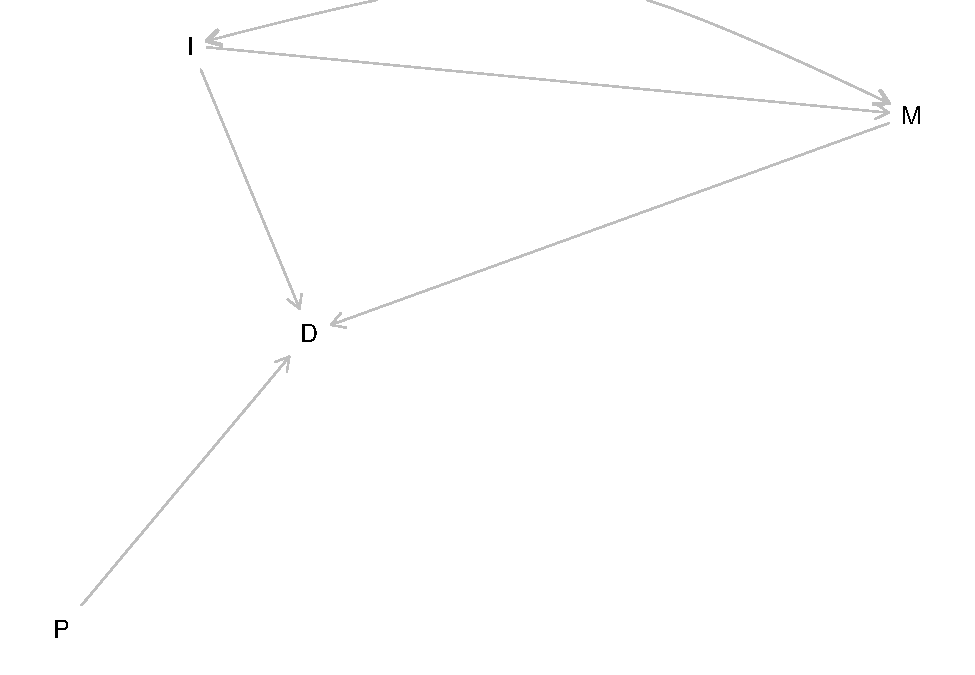
\includegraphics{ii_files/figure-latex/pimdgraph-1.pdf}

\hypertarget{data}{%
\section{Data}\label{data}}

We use the same data as before, based on the analysis in \citet{haggard2012inequality}, but now rather than implementing analysis case by case, the joint distribution of the data will become important for training the model. Here is a snapshot of the data:

\begin{tabular}{l|r|r|r|r}
\hline
Case & P & I & M & D\\
\hline
Afghanistan & NA & 1 & NA & 0\\
\hline
Albania & 0 & 0 & 1 & 1\\
\hline
Algeria & NA & 0 & NA & 0\\
\hline
Angola & NA & 1 & NA & 0\\
\hline
Argentina & 0 & 0 & 1 & 1\\
\hline
Bangladesh & 0 & 0 & 0 & 1\\
\hline
\end{tabular}

Note that although data is gathered on \(D\) and \(I\) in all cases, data on mobilization, \(M\), and external pressure, \(P\), was only gathered for some (in fact, for those cases in which there was democratization). \(M\) in particular derives from qualitative research that assessed whether mobilization took place in those cases that democratized.

The raw correlations berween variables is as shown in Table \ref{pimdcorr}. Note that some of these correlations are missing because data was only gathered on some variables conditional on the values of others. For those quantities where do see correlations they are not especially strong. There is a weak relation between inequality and democratization -- though this is consistent with inequality having different types of effect. the strongest correlation here is between \(P\) and \(M\), which are assumed to be uncorrelated in the model, though this correlation is also quite weak.

\begin{verbatim}
## Warning in cor(data[, -1], use =
## "pairwise.complete.obs"): the standard deviation is
## zero
\end{verbatim}

\begin{tabular}{l|r|r|r|r}
\hline
  & P & I & M & D\\
\hline
P & 1.000 & 0.157 & -0.177 & NA\\
\hline
I & 0.157 & 1.000 & 0.114 & -0.154\\
\hline
M & -0.177 & 0.114 & 1.000 & NA\\
\hline
D & NA & -0.154 & NA & 1.000\\
\hline
\end{tabular}

\hypertarget{inference}{%
\section{Inference}\label{inference}}

With data and model in hand we can update our model to get posteriors on the distribution of all admissible causal types. In practice this is done by constructing a \texttt{stan} model that maps from a set of parameters to a distribution on causal types which in turn provide a likelihood function for observable data. (Using the \texttt{gbiqq} package the posterior is calculated by \texttt{gbiqq(model,\ data)})

The parameters

\begin{Shaded}
\begin{Highlighting}[]
\NormalTok{param_mat <-}\StringTok{ }\KeywordTok{get_parameter_matrix}\NormalTok{(model)}
\KeywordTok{dim}\NormalTok{(param_mat)}
\end{Highlighting}
\end{Shaded}

\begin{verbatim}
## [1]  29 240
\end{verbatim}

\hypertarget{did-inequality-cause-democracy}{%
\subsection{\texorpdfstring{Did inequality \emph{cause} democracy?}{Did inequality cause democracy?}}\label{did-inequality-cause-democracy}}

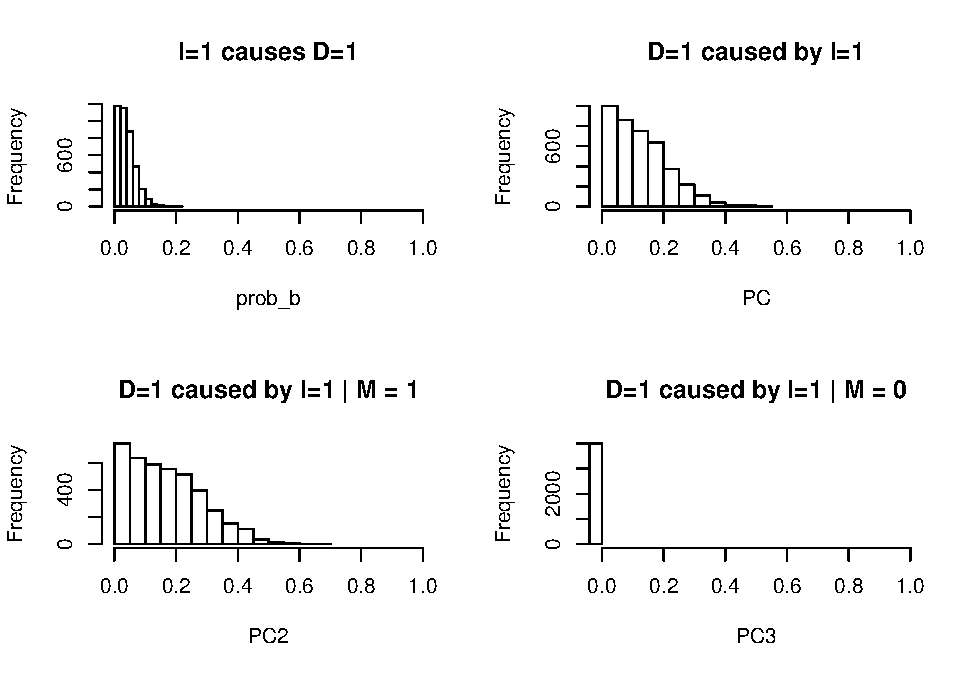
\includegraphics{ii_files/figure-latex/mixedhet-1.pdf}

\hypertarget{did-inequality-prevent-democracy}{%
\subsection{\texorpdfstring{Did inequality \emph{prevent} democracy?}{Did inequality prevent democracy?}}\label{did-inequality-prevent-democracy}}

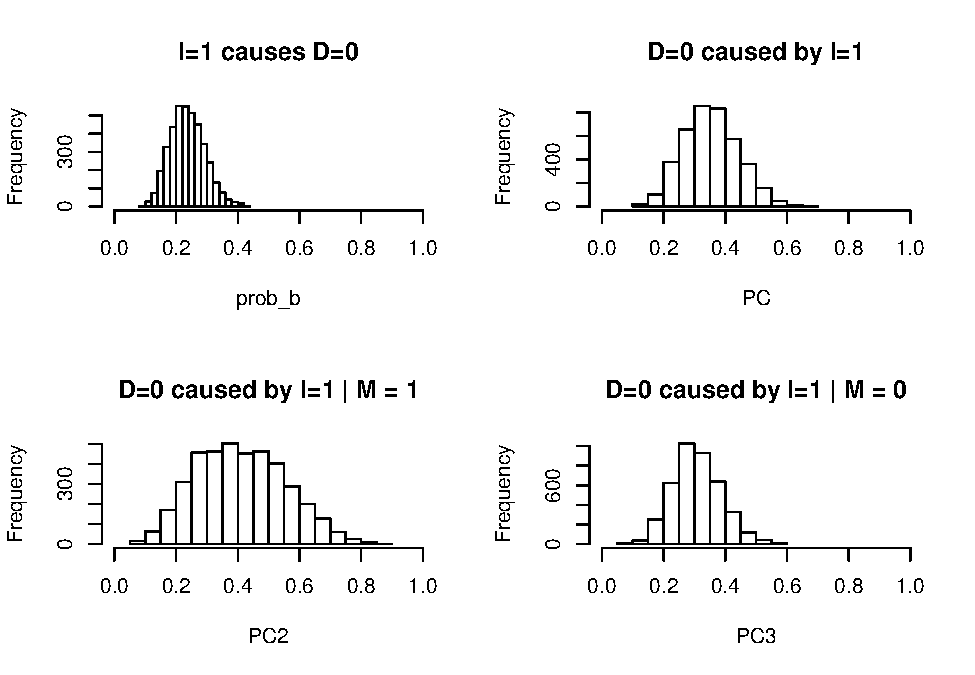
\includegraphics{ii_files/figure-latex/mixedhist2-1.pdf}

We see that inequality appears more likely to prevent democratization than to cause it. We are most confident that inequality played a preventative role in those cases in which there was mobilization but still no democratization. We are most confident that inequality had a positive effect in those cases in which we observe mobilization---but even then the probability that inequality made the difference is small.

\hypertarget{prior-posterior-comparison-for-multiple-estimands}{%
\section{Prior / posterior comparison for multiple estimands}\label{prior-posterior-comparison-for-multiple-estimands}}

Estimands can be calculated for both the prior and posterior distributions.

Inequality causes democratization:

\begin{table}[t]

\caption{\label{tab:unnamed-chunk-62}Prior}
\centering
\begin{tabular}{l|l|l|r|r}
\hline
Query & Subset & Using & mean & sd\\
\hline
not named & All & priors & 0.270 & 0.081\\
\hline
not named & D==1 \& I==1 & priors & 0.466 & 0.149\\
\hline
not named & D==1 \& I==1 \& M ==1 & priors & 0.496 & 0.173\\
\hline
not named & D==1 \& I==1 \& M==0 & priors & 0.403 & 0.131\\
\hline
\end{tabular}
\end{table}

\begin{table}[t]

\caption{\label{tab:unnamed-chunk-62}Posterior}
\centering
\begin{tabular}{l|l|l|r|r}
\hline
Query & Subset & Using & mean & sd\\
\hline
not named & All & posteriors & 0.283 & 0.090\\
\hline
not named & D==1 \& I==1 & posteriors & 0.430 & 0.107\\
\hline
not named & D==1 \& I==1 \& M ==1 & posteriors & 0.419 & 0.154\\
\hline
not named & D==1 \& I==1 \& M==0 & posteriors & 0.440 & 0.104\\
\hline
\end{tabular}
\end{table}

Inequality prevents democratization:

\begin{table}[t]

\caption{\label{tab:unnamed-chunk-63}Prior}
\centering
\begin{tabular}{l|l|l|r|r}
\hline
Query & Subset & Using & mean & sd\\
\hline
not named & All & priors & 0.048 & 0.043\\
\hline
not named & D==0 \& I==1 & priors & 0.127 & 0.117\\
\hline
not named & D==0 \& I==1 \& M ==1 & priors & 0.154 & 0.132\\
\hline
not named & D==0 \& I==1 \& M==0 & priors & 0.000 & 0.000\\
\hline
\end{tabular}
\end{table}

\begin{table}[t]

\caption{\label{tab:unnamed-chunk-63}Posterior}
\centering
\begin{tabular}{l|l|l|r|r}
\hline
Query & Subset & Using & mean & sd\\
\hline
not named & All & posteriors & 0.027 & 0.026\\
\hline
not named & D==0 \& I==1 & posteriors & 0.085 & 0.081\\
\hline
not named & D==0 \& I==1 \& M ==1 & posteriors & 0.114 & 0.104\\
\hline
not named & D==0 \& I==1 \& M==0 & posteriors & 0.000 & 0.000\\
\hline
\end{tabular}
\end{table}

\hypertarget{discussion}{%
\section{Discussion}\label{discussion}}

\hypertarget{part-design-choices}{%
\part{Design Choices}\label{part-design-choices}}

\hypertarget{elements-of-design}{%
\chapter{Elements of Design}\label{elements-of-design}}

\begin{center}\rule{0.5\linewidth}{\linethickness}\end{center}

A fully specified causal model includes the information needed to assess the properties of a research design that seeks to learn from or learn about the model. We talk through how to go from defining causal models to ``declaring'' research designs and use this framework in later chapters to inform decisions about details of design choices.

\begin{center}\rule{0.5\linewidth}{\linethickness}\end{center}

So far we have described a way to think about causal models, a way to specify causal estimands, and a Bayesian approach to inference, given models and estimands. Together with a strategy for data gathering these elements are enough to fully characterize a research design. If in addition we provide criterea for evaluating a design we have enough to be able to simulate the behavior of a research design and assess whether a design is up to the task fo answering the questions we want to answer.

Once we have a method to assess the performance of a given design we can can start asking what kind of design is optimal, given some beliefs about the world (see \citet{blair2016declaring} for more on this general approach to design declaration and diagnosis). In the next chapters we use this approach to assess a set of design choices including choices regarding the clues about which data is sought, the types of cases for which data is sought, and the number of cases for which different types of data is sought.

In the remainder of this chapter we discuss a simple evaluative criterion for a design and give examples for design declaration for a simple single case process tracing design and a mixed methods design.

\hypertarget{declaring-a-process-tracing-design}{%
\section{Declaring a process tracing design}\label{declaring-a-process-tracing-design}}

\hypertarget{steps}{%
\subsection{Steps}\label{steps}}

We use the MIDA approach (model, inquiry, data strategy, answer strategy) approach to declare a simple process tracing design with an arbitrary model.

\begin{itemize}
\item
  \textbf{Model.} We will define a model as introduced in Chapter 2. For this we need to define:

  \begin{itemize}
  \tightlist
  \item
    A directed acyclic graph. In doing so we declare the set of variables we are interested and the relations of independence between them. In defining the variables we generally also define the ranges of the variables---indicating, for example whether they are binary, categorical, or continuous. In defining the edges we identify the set of parents of any node.
  \item
    Any restrictions on functional forms relating parents to children. In the binary set up, imposing functional form assumptions is the same as restructuring causal types.
  \item
    A declaration of structures of unobserved confounding.\\
  \item
    Priors. Beliefs about the distribution of shocks. When defined as part of the model we think of these priors as being the priors from the vantage point of someone assessing a design and they need not be the same as the priors used in the analysis.
  \end{itemize}
\item
  \textbf{Inquiry} As discussed in Chapter 4, an inquiry is a question asked of a model. This is typically a question about the distribution of a variable in some controlled or natural condition, or some summary of such distributions. We refer to the quantity being targeted by a query as the estimand.
\item
  \textbf{Data strategy.} The data strategy describes how data will be gathered. In typical \texttt{DeclareDesign} applications this includes both randomization and data gathering (sampling) strategies. We focus on data gathering though we highlight that randomization strategies can be implemented via a modification of the confounds allowed by the model. A sampling strategy might indicate a sequence of conditional data gathering schemes, for instance: gather data on \(X\) and \(Y\) for 100 cases, then gather data on \(M\) for all cases in which \(X=Y\).
  Note that in some cases we might want to think of the estimand as being defined \emph{after} the data strategy. This would be the case for instance if we chose a case and we seek to work out some feature \emph{about that case} rather than about the population.
\item
  \textbf{Answer strategy}. The answer strategy combines the observed data with a causal model to generate an updated model from which inferences can be drawn. Importantly, the model used in the answer strategy does not need to be the same model as assumed at the model step since we could imagine analysts coming to the data with quite different models in mind. Of course any model used in the answer strategy should generally involve the same variables as in the model itself.
\end{itemize}

A design is a concatenation of these four steps.

The concatenated lets us examine instances of the application of a design. A single instance would involve

\begin{enumerate}
\def\labelenumi{\arabic{enumi}.}
\tightlist
\item
  a single draw of a true parameter vector from the distribution given in the model definition
\item
  a calculation of the value of an estimand given this true parameter draw
\item
  the generation of a dataset given the model implied by step 1 and the data strategy
\item
  the generation of an answer to the inquiry generated from the realized data from 3. and the answer strategy
\end{enumerate}

With the observation of multiple instances we get to assess the distribution of our answers --- and our uncertainty around these -- over repeated draws, and each time we get to see how well the answer we get maps onto the assumed truth in that draw.

\hypertarget{illustration-in-code}{%
\subsection{Illustration in code}\label{illustration-in-code}}

In the \texttt{gbiqq} package there is a single function that lets you declare a full design in one go by letting you supply arguments to declare a model, an inquiry, a data strategy, and an answer strategy

\begin{Shaded}
\begin{Highlighting}[]
\CommentTok{# A single function can be used to declare a model, an inquiry, a data strategy, and an answer strategy}

\NormalTok{my_design <-}\StringTok{ }\KeywordTok{gbiqq_designer}\NormalTok{(}
  
   \DataTypeTok{model           =} \KeywordTok{make_model}\NormalTok{(}\StringTok{"X -> M -> Y"}\NormalTok{),}
   \DataTypeTok{inquiry         =} \KeywordTok{list}\NormalTok{(}\DataTypeTok{ATE =} \StringTok{"Y[X=1] - Y[X=0]"}\NormalTok{),}
   \DataTypeTok{data_strat      =} \KeywordTok{list}\NormalTok{(}\DataTypeTok{n_obs =} \DecValTok{5}\NormalTok{, }
                          \DataTypeTok{vars =} \KeywordTok{list}\NormalTok{(}\KeywordTok{c}\NormalTok{(}\StringTok{"X"}\NormalTok{, }\StringTok{"Y"}\NormalTok{), }\StringTok{"M"}\NormalTok{), }
                          \DataTypeTok{probs =} \KeywordTok{list}\NormalTok{(}\DecValTok{1}\NormalTok{, }\FloatTok{.5}\NormalTok{), }
                          \DataTypeTok{subsets =} \KeywordTok{list}\NormalTok{(}\OtherTok{NULL}\NormalTok{, }\StringTok{"X==1 & Y==0"}\NormalTok{),}
                          \DataTypeTok{n =} \OtherTok{NULL}\NormalTok{),}
   \DataTypeTok{answer_strat  =} \OtherTok{NULL}
\NormalTok{)}
\end{Highlighting}
\end{Shaded}

With this model in hand you can use it to draw likely data, run analyses, an drun diagnostics.

\begin{Shaded}
\begin{Highlighting}[]
\NormalTok{sample_data      <-}\StringTok{ }\KeywordTok{draw_data}\NormalTok{(my_design)}
\NormalTok{sample_estimands <-}\StringTok{ }\KeywordTok{draw_estimands}\NormalTok{(my_design)}
\NormalTok{sample_estimates <-}\StringTok{ }\KeywordTok{get_estimates}\NormalTok{(my_design, df)}
\end{Highlighting}
\end{Shaded}

\hypertarget{diagnosands-evaluating-a-model}{%
\subsection{Diagnosands: Evaluating a model}\label{diagnosands-evaluating-a-model}}

The observation that theories vary in their precision points to a method for describing the learning that is attributable to a lower-level theory relative to a higher level theory. When a lower-level theory represents a disaggregation, the lower-level theory identifies a set of potentially observable variables that are not listed by the the higher-level theory. This allows one to assess the gains in precision (for some collection of unobserved variables) that can arise from learning the values of additional observables in the lower-level theory.

Suppose that the contribution of a lower-level theory is to allow for inferences from new data \(K\) about some set of query variables \(Q\), after we have already observed variables \(W\) from the higher-level model.

Then we can use the expected squared error from the mean posterior estimate as a measure of precision for collection \(Q\), as a measure of loss:

\[E_{k, q} \left(\left( \int q' P(q' | k, w)dq' - q\right)^2\right)\]
where the expectation is taken over the joint distribution of \(K\) and \(Q\), given \(W\). This is an expected loss---or the \emph{Bayes risk}. The inner term \(P(q'|k, w)\) is the posterior distribution on \(q'\) given observation of \(k\) and \(w\).

Another way to think of the gains is as the expected reduction in the variance of the Bayesian posterior: how certain do you expect you will be after you make use of this new information?

In fact these two quantities are equivalent (see for example \citet{scharf1991statistical}). Moreover, it is easy to see that whenever inferences are sensitive to \(K\), the expected variance of the posterior will be lower than the variance of the prior. This can be seen from the law of total variance, written here to highlight the gains from observation of \(K\), given what is already known from observation of \(W\).\footnote{A similar expression can be given for the expected posterior variance from learning \(K\) in addition to \(W\) when \(W\) is not yet known. See, for example, Proposition 3 in \citet{geweke2014analysis}.}\\
\[Var(Q|W) = E_{K|W}(Var(Q|K,W)) +Var_{K|W}(E(Q|K,W))\]

The contribution of a theory can then be defined as the mean reduction in Bayes risk:

\[\text{Gains from theory} = 1- \frac{E_{K|W}(Var(Q|K,W))}{Var(Q|W)}\]

This is a kind of \(R^2\) measure (see also \citet{gelman2006bayesian}).

Other loss functions could be used, including functions that take account of the costs of collecting additional data,\footnote{Further, one might call into question the value of a theory if the gains in precision depend upon data that are practically impossible to gather.} or to the risks associated with false diagnoses.\footnote{For instance, in \citet{heckerman1991toward}, an objective function is generated using expected utility gains from diagnoses generated based on new information over diagnoses based on what is believed already. In their treatment \citep[Equation 6]{heckerman1991toward}, the expected value of new information \(K\), given existing information \(W\) is: \(\sum{K}P(K|W)( EU(d(Q,W,K)|W, K) - EU(d(Q, W)|W, K))\) where \(EU\) is expected utility and \(d\) is the optimal inference (diagnosis) given available data. Note that the diagnosis can take account of \(K\) when it is observed, but the expected utility depends on \(K\) whether or not it is observed, as \(K\) carries information about the state of interest.}

For illustration say that it is known that \(X=1, Y=1\) and that, given this information (playing the role of \(W\)), the posterior probability that a unit is of type \(b\) (and not type \(d\)) is \(p\). Say then that a theory specifies that \(K\) will take a value 1 with probability \(\phi_j\) if the unit is of type \(j\). Then what is the value added of this theory? Define \(Q\) here as the query regarding whether the unit is a \(b\) type. Then the prior variance, \(Var(Q|W)\), is simply \(p(1-p)^2 +(1-p)p^2 = p(1-p)\).

To calculate \(E_{K|W}(Var(Q|K,W))\), note that the posterior if \(K\) is observed is \(\frac{\phi_bp}{\phi_bp+\phi_d(1-p)}\). Let us call this \(\hat{q}_K\), and the belief when \(K\) is not observed \(\hat{q}_{\overline{K}}\).
In that case the \emph{expected error} is:

\[\text{Expected Error} = p\phi_b\left(1-\hat{q}_K\right)^2+(1-p)\phi_d\hat{q}_K^2+p(1-\phi_b)\left(1-\hat{q}_{\overline{K}}\right)^2+(1-p)(1-\phi_d)\hat{q}_{\overline{K}}^2\]

where the four terms are the errors when \(K\) is seen for a \(b\) type, when \(K\) is seen for a \(d\) type, when \(K\) is not seen for a \(b\) type, and when \(K\) is not see for a \(d\) type.

Defining \(\rho_K = (p\phi_b+(1-p)\phi_d)\) as the probability of observing \(K\) given the prior, we can write the posterior variance as:

\[\text{Expected Posterior Variance} = \rho_K\hat{q}_K(1-\hat{q}_K)+(1-\rho_K)\hat{q}_{\overline{K}}(1-\hat{q}_{\overline{K}})\]

With a little manipulation, both of these expressions simplify to:

\[\text{Expected Posterior Variance} =p(1-p)\left(\frac{\phi_b\phi_d}{\phi_bp+\phi_d(1-p)} + \frac{(1-\phi_b)(1-\phi_d)}{(1-\phi_b)p+(1-\phi_d)(1-p)}\right)\]

The gains are then:

\[\text{Gains} =1- \frac{\phi_b\phi_d}{\phi_bp+\phi_d(1-p)} - \frac{(1-\phi_b)(1-\phi_d)}{(1-\phi_b)p+(1-\phi_d)(1-p)}\]

Let's consider the same question using a particular model and calculate these quantities given this model.

\begin{Shaded}
\begin{Highlighting}[]
\NormalTok{model <-}\StringTok{ }\KeywordTok{make_model}\NormalTok{(}\StringTok{"X -> Y; K -> Y"}\NormalTok{) }\OperatorTok
\StringTok{         }\KeywordTok{set_parameters}\NormalTok{(}\KeywordTok{c}\NormalTok{(}
           \FloatTok{.5}\NormalTok{, }\FloatTok{.5}\NormalTok{, }
           \FloatTok{.5}\NormalTok{, }\FloatTok{.5}\NormalTok{, }
           \DecValTok{0}\NormalTok{,.}\DecValTok{5}\NormalTok{,}\DecValTok{0}\NormalTok{,}\DecValTok{0}\NormalTok{, }\DecValTok{0}\NormalTok{,}\DecValTok{0}\NormalTok{,}\DecValTok{0}\NormalTok{,}\DecValTok{0}\NormalTok{, }\DecValTok{0}\NormalTok{,}\DecValTok{0}\NormalTok{,}\DecValTok{0}\NormalTok{,}\DecValTok{0}\NormalTok{, }\DecValTok{0}\NormalTok{,}\DecValTok{0}\NormalTok{,}\DecValTok{0}\NormalTok{,.}\DecValTok{5}\NormalTok{))}
\end{Highlighting}
\end{Shaded}

The probability that \(K=1\) given \(X=Y=1\) is:

\begin{Shaded}
\begin{Highlighting}[]
\NormalTok{prob_K <-}\StringTok{ }\KeywordTok{estimand_distribution}\NormalTok{(model, }
                   \DataTypeTok{query =} \StringTok{"K[Y=1]==1"}\NormalTok{,}
                   \DataTypeTok{using =} \StringTok{"parameters"}\NormalTok{, }
                   \DataTypeTok{subset =} \StringTok{"X==1 & Y==1"}\NormalTok{)}
\end{Highlighting}
\end{Shaded}

The inferences conditional on the observation of \(K\) are:

\begin{Shaded}
\begin{Highlighting}[]
\NormalTok{inferences <-}\StringTok{ }\NormalTok{gbiqq}\OperatorTok{::}\KeywordTok{get_estimands}\NormalTok{(}
\NormalTok{                   model, }
                   \DataTypeTok{queries =} \StringTok{"Y[X=1]>Y[X=0]"}\NormalTok{,}
                   \DataTypeTok{using =} \StringTok{"parameters"}\NormalTok{, }
                   \DataTypeTok{subsets =} \KeywordTok{list}\NormalTok{(}\StringTok{"X==1 & Y==1"}\NormalTok{, }\StringTok{"X==1 & Y==1 & K==1"}\NormalTok{, }\StringTok{"X==1 & Y==1 & K==0"}\NormalTok{))}
\end{Highlighting}
\end{Shaded}

The expected error is then reduced from 0 to
0

\hypertarget{other-measures-of-a-gain-from-a-theory}{%
\subsection{Other measures of a gain from a theory}\label{other-measures-of-a-gain-from-a-theory}}

Other natural measures of gains from theory might include the simple correlation between \(K\) and \(Q\), or entropy-based measures (see \citet{zhang2003properties} for many more possibilities).

For this problem the correlation is given by (see appendix):

\[\rho_{KQ} = \frac{(\phi_b+\phi_d)(1-2p)(p(1-p))^{.5}}{
(p\phi_b+(1-p)\phi_d)(1-(p\phi_b+(1-p)\phi_d)))^{.5}}\]

One might also use a measure of ``mutual information'' from information theory:

\[I(Q,K) = \sum_q \sum_k P(q,k)\log\left(\frac{P(q,k)}{P(q)P(k)}\right)\]

To express this mutual information as a share of variation explained, we could divide \(I(Q,K)\) by the entropy of \(Q\), \(H(Q)\) where \(H(Q) = -\sum_qP(q)\log(P(q))\). The resulting ratio can be interpreted as 1 minus the ratio of the entropy of \(Q\) conditional (on \(K\)) to the unconditional entropy of \(Q\).

For this example, Figure \ref{fig:probative_value} shows gains as a function of \(\phi_b\) given a fixed value of \(\phi_d\). The figure also shows other possible measures of probative value, with, in this case, the reduction in entropy tracking the reduced posterior variance closely.

\begin{figure}

{\centering 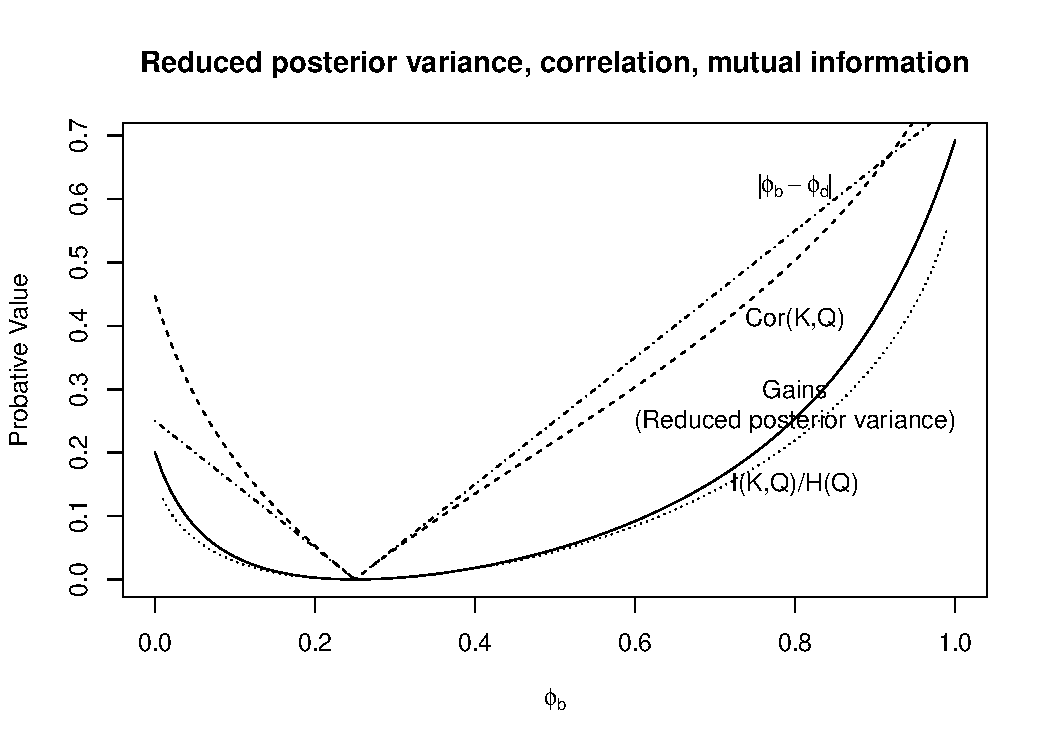
\includegraphics[width=.7\textwidth]{ii_files/figure-latex/unnamed-chunk-71-1} 

}

\caption{\label{fig:probative_value} The solid line shows gains in precision (reduced posterior variance) for different values of $\phi_b$ given $\phi_d=0.25$ and $p=.5$ for the example given in the text. Additional measures of probative value are also provided including $|\phi_b - \phi_d|$, the correlation of $K$ and $Q$, and the reduction in entropy in $Q$ due to mutual information in $Q$ and $K$.}\label{fig:unnamed-chunk-71}
\end{figure}

\hypertarget{declaring-a-mixed-methods-design}{%
\section{Declaring a mixed methods design}\label{declaring-a-mixed-methods-design}}

\hypertarget{model}{%
\subsection{Model}\label{model}}

\hypertarget{data-strategies}{%
\subsection{Data strategies}\label{data-strategies}}

\hypertarget{estimands}{%
\subsection{Estimands}\label{estimands}}

\hypertarget{answer-strategies}{%
\subsection{Answer Strategies}\label{answer-strategies}}

\begin{Shaded}
\begin{Highlighting}[]
\CommentTok{# detach(package:DeclareDesign, unload=TRUE)}
\end{Highlighting}
\end{Shaded}

\hypertarget{clue-selection-as-a-decision-problem}{%
\chapter{Clue Selection as a Decision Problem}\label{clue-selection-as-a-decision-problem}}

\begin{center}\rule{0.5\linewidth}{\linethickness}\end{center}

We draw out the implications of the causal model approach for clue selection strategies. We introduce a tool for generating an optimal decision tree for clue selection given.

\begin{center}\rule{0.5\linewidth}{\linethickness}\end{center}

Consider now the problem of determining what qualitative data to gather on a case. Evidently it makes sense to gather information on clues that have large probative value, but whether or not clues have probative value can depend on what clues have already been collected: Finding out that the Butler had no motive may be informative for the claim that he is innocent, but it may not be useful if you already know he had no opportunity.

In our running example, we can see many situations where researchers have a choice of observations that could be informative, and situations in which the informativeness of an observation can depend on what is already known. In Figure \ref{fig:running}, we showed how one can use the structural equations to provide a set of conditional causal graphs that let one see easily what caused what at different values of the root nodes \(S\) and \(X\). Each of these plots graphs a particular context. We can thus readily see which collection of root nodes constitutes a given query, or estimand. Turning things around, we can see, given a query, which nodes are informative of the probability that the query is true.\footnote{With larger graphs, continuous variables, and more stochastic components, it may not be feasible to graph every possible context; but the strategy for inference remains the same.}

For example, suppose one can see that \(X=0\) and \(Y=0\) but does not know the causal effect of \(X\) on \(Y\) This is equivalent to saying that we know that we are in either panel \(A\) or \(B\) but we do not know which one. Defining the query in terms of root nodes, the question becomes \(S \stackrel{?}{=} 1\), or \(P(S=1|X=0,Y=0)\); the difference between the contexts in the two panels is that \(S=0\) when, and only when, \(X=0\) causes \(Y=0\) . Given the structural equation for \(S\), \(P(S|X=0,Y=0) = P(S|X=0)\), and given independence of \(X\) and \(S\), \(P(S=1|X=0)= \pi^S\). Figuring out \(S\) fully answers the query: that is, given what we know already, \(S\) is doubly decisive for the proposition.\footnote{Graphically what is important is that \(S\) is informative not because it is \(d-\)connected with \(Y\), but because it is \(d-\)connected to the query variable---here, simply, to itself.}

We can also see instances in this example of how existing data can make clues uninformative. Say one wanted to know if \(X\) causes \(C\) in a case. As we can see from inspection of the panels, this query is equivalent to asking whether \(S=1\) (as \(X\) causes \(C\) only in those two panels (\(B\) and \(D\)) where \(S=1\). Data on \(R\) is unconditionally informative about this query as \(R\) is not \(d-\)separated from \(S\). For example, \(R=1\) implies \(S=0\). However, if \(C\) and \(X\) are already known, then \(R\) is no longer informative because \(C\) and \(X\) together \emph{d}-separate \(R\) from \(S\).\footnote{We can come to the same conclusion by reasoning with the graphs: if \(X=0\) and \(C=1\), we know we are in subfigure \(A\) or \(B\), and \(X\) causes \(C\) only in panel \(B\). However, \(R\) is of no help to us in distinguishing between the two contexts as it takes the same value in both graphs.}

The running example also lets us demonstrate how informative clues can be found in many different places in a graph.

\begin{enumerate}
\def\labelenumi{\arabic{enumi}.}
\item
  \textbf{Informative spouses} Spouses---parents of the same child---can inform on one another. As we have seen in other examples, when an outcome has multiple causes, knowing the value of one of those causes helps assess the effect(s) of the other(s). For example, here, \(S\) and \(X\) are both parents of \(C\); \(S\) is thus informative for assessing whether \(X\) causes \(C\). Indeed this query, written in terms of roots, is simply \(P(S)\): \(X\) causes \(C\) if and only if \(S=1\). Likewise, \(S\) causes \(C\) (negatively) if and only if \(X=1\).
\item
  \textbf{Pre-treatment clues.} Did the absence of media reports on corruption (\(R=0\)) cause government survival (\(Y=0\))? Look to the pre-treatment clue, \(X\): \(X=0\) is a smoking gun establishing that the absence of a report produced government survival. Or, substantively, if there were a free press, then a missing report would never be a cause of survival since it would occur only in the absence of corruption, which would itself be sufficient for survival. More broadly, this example illustrates how knowledge of selection into treatment can be informative about treatment effects.
\item
  \textbf{Post-outcome clues.} Suppose we observe the presence of a free press (\(X=1\)) and want to know if it caused a lack of corruption (\(C=0\)), but cannot observe the level of corruption directly. Observing \(Y\)---which occurs after the outcome---is informative here: if \(X=1\), then \(X\) causes \(C\) (negatively) if and only if \(Y=0\). When an outcome is not observed, a consequence of that outcome can be informative about its value and, thus, about the effect of an observed suspected cause.
\item
  \textbf{Mediators as clues}: We see a politically sensitive government (\(S=1\)) and its survival (\(S=0\)). Did the government survive because of its sensitivity to public opinion? Here, the mediation clue \(C\) is helpful: a lack of corruption, \(C=0\), is evidence of \(S\)'s negative effect on \(Y\). --\textgreater{}
\end{enumerate}

And of course, different clues can be informative in different ways for different types of estimand.

Needed then is a systematic way for identifying what clues to look for, and perhaps, in what order to look for them.

\hypertarget{a-strategic-approach}{%
\section{A strategic approach}\label{a-strategic-approach}}

The representation of inference problems as one of querying a Bayesian model points to a relatively simple method for answering this question, at least for small problems. Consider first a situation where one has access to data \(W\) and wants to know the expected probative value of all possible collections of data one could gather.

This can be done as follows:

\begin{enumerate}
\def\labelenumi{\arabic{enumi}.}
\tightlist
\item
  First define a model, including a signature \(S = (\mathcal{U}, \mathcal{V}, \mathcal{R})\), structural equations \(\mathcal{F}\), and beliefs on \(\mathcal{U}\), \(P()\).
\item
  Second, define a query on the model, as a statement about values of \(\mathcal{V}\) given different \(\mathbb{do}\) operations.
\item
  Third, use \(P\) to draw a vector of \(U\) values and assess whether the query is true or not given \(U\) and whether \(W\) obtains. Then, over many repeated draws from \(P\) calculate the \emph{share} of times that the query is true among those cases in which \(W\) is true. This gives posterior probability on \(Q\), \(P(Q|W)\).
\item
  Fourth, given posterior \(P(Q|W)\) calculate the probability of observing any realization of values \(K'\) given the set of clues sought. For each possible realization calculate posterior variance using \(P(Q|W, K')\), itself calculated as the share of draws in which the query is true given both \(W\) and the particular set of findings \(K'\) obtains. Calculate the \emph{expected} posterior variance by taking an average of these variances with weights given by the probability of observing the clue pattern in question.
\item
  Repeat step 4 for all possible collections of clues that one could search for.
\end{enumerate}

This procedure then returns expected posterior variance associated with a planned search for a collection of clues. A more sophisticated strategy would determine which clues to search for later given findings from clues that are sought first. This reflects the possibility that a given clues \(K_2\) may be informative if another clue \(K_1\) turns up positive but not if it comes out negative.

We provide some tools for both of these approaches and illustrate them below.

\hypertarget{clue-selection-for-the-running-example}{%
\section{Clue selection for the running example}\label{clue-selection-for-the-running-example}}

Lets return to the running example and assess the informativeness of different clue strategies.

Recall that a model consists of an ordered set of variables \(V\), a set of exogenous variables \(U\), with a distribution over these, given by \(P(u)\) and a set of functions, one for each \(V\in\mathcal{V}\), \(f_v(v',u_v)\) which takes as arguments a subset of variables in \(\mathcal{V}\) that must be prior to \(V\) in the ordering plus an element of \(U\) associated with \(V\).

TRANSITIONAL TEXT LINKING FROM LAST CHAPTER

In the same way we can figure out outcomes for all possible profiles of data one might have on \(m\) binary variables. With five variables there are 243 (\(3^5\)) combinations of 0s, 1s and unknowns. We provide a function which allows specific examines or else examinations of the form ``all strategies that seek up to \(m_k\) clues when up to \(m_w\) variables are already observed.''

\begin{Shaded}
\begin{Highlighting}[]
\NormalTok{model <-}\StringTok{ }
\StringTok{  }
\StringTok{  }\KeywordTok{make_model}\NormalTok{(}\StringTok{"S -> C -> Y <- R <- X; X -> C -> R"}\NormalTok{) }\OperatorTok
\StringTok{  }
\StringTok{  }\KeywordTok{set_restrictions}\NormalTok{(}\DataTypeTok{node_restrict =} \KeywordTok{list}\NormalTok{(}\DataTypeTok{C =} \StringTok{"C1110"}\NormalTok{, }\DataTypeTok{R =} \StringTok{"R0001"}\NormalTok{, }\DataTypeTok{Y =} \StringTok{"Y0001"}\NormalTok{), }\DataTypeTok{action =} \StringTok{"keep"}\NormalTok{)}

\KeywordTok{plot_dag}\NormalTok{(model)}
\end{Highlighting}
\end{Shaded}

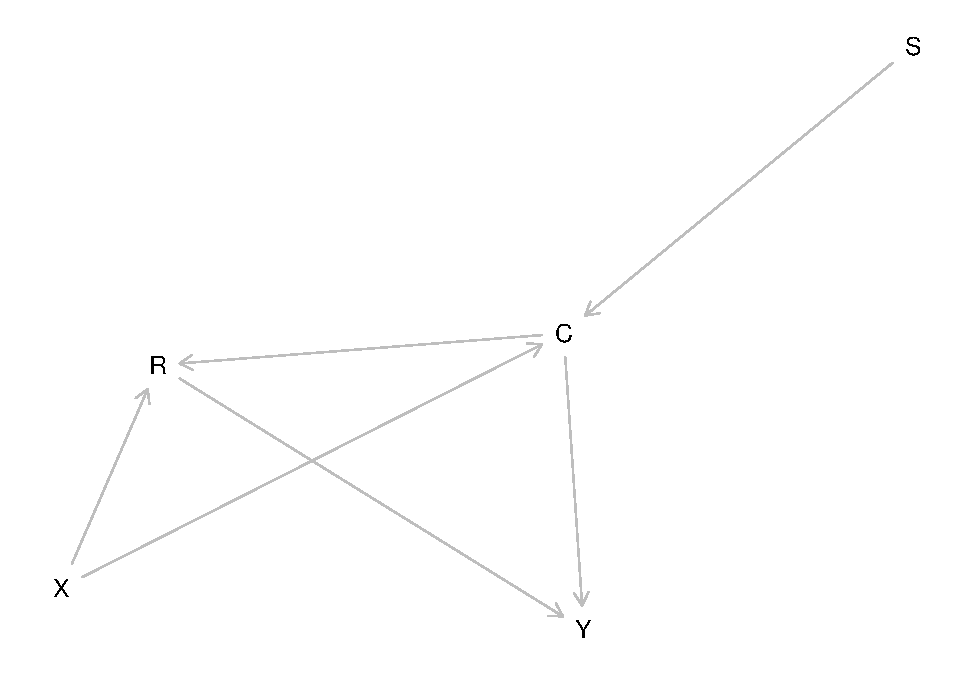
\includegraphics{ii_files/figure-latex/ch11strategies_chunk_slowxx-1.pdf}

This produces a matrix shown here as table \ref{tab:showstrats5xx} for a situation in which \(S=0\) and \(Y=0\) is already observed.

\begin{table}[t]

\caption{\label{tab:showstrats5xx}A fragment of the table of expected posterior variance for all two clue strategies given observations on two nodes. Firs column gives prior variance, second gives variance condition on data pattern $W$, as indicated by row labels; subsequent columns give expected variance when different clues are sought. }
\centering
\begin{tabular}{l|r|r|r|r|r|r|r}
\hline
  & S & X & C & R & Y & posterior & prob\\
\hline
1 & 0 & NA & NA & NA & 1 & 1 & 0.25\\
\hline
3 & 0 & 1 & NA & NA & 1 & 1 & 0.25\\
\hline
7 & 0 & NA & 1 & NA & 1 & 1 & 0.25\\
\hline
9 & 0 & 1 & 1 & NA & 1 & 1 & 0.25\\
\hline
19 & 0 & NA & NA & 1 & 1 & 1 & 0.25\\
\hline
21 & 0 & 1 & NA & 1 & 1 & 1 & 0.25\\
\hline
25 & 0 & NA & 1 & 1 & 1 & 1 & 0.25\\
\hline
27 & 0 & 1 & 1 & 1 & 1 & 1 & 0.25\\
\hline
\end{tabular}
\end{table}

From there it is easy to assess the \emph{expected} gains from seeking any kind of clue. See Table \ref{tab:scxrylearning}

\begin{tabular}{l|l|l|l|l}
\hline
Strategy & Given & Prior belief & Prior Uncertainty & Posterior Uncertainty\\
\hline
S & X==0 \& Y==0 & 0.5 & 0.25 & 0\\
\hline
C & X==0 \& Y==0 & 0.5 & 0.25 & 0.25\\
\hline
R & X==0 \& Y==0 & 0.5 & 0.25 & 0.25\\
\hline
C, R & X==0 \& Y==0 & 0.5 & 0.25 & 0.25\\
\hline
C, S & X==0 \& Y==0 & 0.5 & 0.25 & 0\\
\hline
S, R & X==0 \& Y==0 & 0.5 & 0.25 & 0\\
\hline
C, S, R & X==0 \& Y==0 & 0.5 & 0.25 & 0\\
\hline
\end{tabular}

In this case if we know \(X=0\) and \(Y=0\) and we are interested in finding out whether\(X=0\) \emph{because} \(Y\) is 0 we should look for evidence on \(S\). Given this simple model, knowledge of \(S\) is enough to answer teh question at hand and no othe information is useful at all.

\hypertarget{dynamic-strategies}{%
\subsection{Dynamic Strategies}\label{dynamic-strategies}}

The clue collection strategies described above assume that researchers identify the full set of clues to be gathered in advance and do not alter their in Given \(n\) nodes, a data collection strategy will be of the form:
\[\sigma = \{K_1, (K_2|K_1 = 1), (K_2|K_1 = 0), (K_3|K_1=1, K_2 =0)\dots\}\]

where each \(K_j\) is en element of the nodes on the graph, or is the empty set. Each of these strategies has an associated expected reduction in variance as well as an associated expected cost. Such a strategy vector specifies the first clue, and then subsequent clues condition on what was found from previous searches. We restrict strategies to those in which each clue is sought at most once (though possibly sought at times that depends on findings), and in which if a clue is sought it is sought immediately. For a risk neutral decision maker, this may be sufficient to choose among them.

In the running example with five binary nodes the strategies needs to specify up to \(2^4\) decision points, reflecting the initial choice and the decisions made after learning about four nodes. An example of a strategy, summarizing contingent plans is the below:

\begin{Shaded}
\begin{Highlighting}[]
\NormalTok{prices <-}\StringTok{ }\FloatTok{.5+.5}\OperatorTok{*}\KeywordTok{runif}\NormalTok{(}\DecValTok{5}\NormalTok{)}

\NormalTok{strategy <-}\StringTok{ }\KeywordTok{random_list_strategy}\NormalTok{(}\DecValTok{5}\NormalTok{)}

\KeywordTok{strategy_cost_benefit}\NormalTok{(  model,  my_operations, my_query, }\DataTypeTok{sims=}\DecValTok{100}\NormalTok{,   }\DataTypeTok{U=}\OtherTok{NULL}\NormalTok{,   }\DataTypeTok{cost =}\NormalTok{ prices,   }\DataTypeTok{strategy =}\NormalTok{ strategy  }\CommentTok{# Or a matrix with one column per node indicating whether to be sought or not}
\NormalTok{  )}
\end{Highlighting}
\end{Shaded}

Note that strategies cannot use information unavailable ex ante. To ensure the right structure we specify the strategy as \(n\) vectors, of length \(1, 2, 4, \dots\). For example of the form \(\{\{1\}, \{2,3\}, \{3, 4, \emptyset, \emptyset\}\}\)

This has the interpretation: seek evidence on node 1 first, if one finds \(V_1=1\) seek evidence on node 2, otherwise seek evidence on node 3, if \(V_1=1\) and \(V_2=1\) seek evidence on node 3, but if \(V_1=1\) and \(V_2=0\) seek \(V_4\), if \(V_3\) is positive stop seeking.

For each strategy we can then assess the expected variance reduction; in addition, if collecting different clues comes at different costs---but collection depends on past findings---then we can also calculated the expected costs of each strategy.

NEED TO REDO STRATEGIES CALCULATIONS

Figure below plots a collection of strategies based on two criteria---the variance reduction and the expected number of clues sought, which could be an indicator for cost. One can see a frontier of optimal strategies, depending on how these two desiderata trade-off against each other.

Below we graph one of these strategies on the frontier (the median strategy on the frontier) as a decision tree. The interpretation is to seek the first clue first; it will be revealed to be present (1) or not(0), a subsequent branch is then chosen depending on what is found and the indicated clue then sought, and so on. (Note currently the strategy sets we examine include ones in which the same clue is sought multiple times)

\hypertarget{clue-selection-for-the-democracy-model}{%
\section{Clue selection for the Democracy model}\label{clue-selection-for-the-democracy-model}}

With a model in hand we are also in a position to assess what we \emph{could} learn from different data stratgies and what we would infer upon discovery of different data.

\begin{verbatim}
## Generated expanded expression:
## (M[I=1] < M[I=0]) |
##             (D[I=1, M=0, P=0] > D[I=0, M=0, P=0] | D[I=1, M=1, P=0] > D[I=0, M=1, P=0] | D[I=1, M=0, P=1] > D[I=0, M=0, P=1] | D[I=1, M=1, P=1] > D[I=0, M=1, P=1]) |
##             (D[M=1, I=0, P=0] < D[M=0, I=0, P=0] | D[M=1, I=1, P=0] < D[M=0, I=1, P=0] | D[M=1, I=0, P=1] < D[M=0, I=0, P=1] | D[M=1, I=1, P=1] < D[M=0, I=1, P=1]) | 
##             (D[P=1, M=0, I=0] < D[P=0, M=0, I=0] | D[P=1, M=1, I=0] < D[P=0, M=1, I=0] | D[P=1, M=0, I=1] < D[P=0, M=0, I=1] | D[P=1, M=1, I=1] < D[P=0, M=1, I=1])
\end{verbatim}

\begin{table}[t]

\caption{\label{tab:unnamed-chunk-80}\label{possible_outcomes} Table shows possible data patterns for P and M given I = 1 and D = 1 together with the probability of observing each data realization given data is sought on a variable and the posterior given that data realization.}
\centering
\begin{tabular}{r|r|r|r|r|r}
\hline
I & P & M & D & posterior & prob\\
\hline
1 & NA & NA & 1 & 0.128 & 0.011\\
\hline
1 & 0 & NA & 1 & 0.231 & 0.003\\
\hline
1 & 1 & NA & 1 & 0.088 & 0.008\\
\hline
1 & NA & 0 & 1 & 0.000 & 0.002\\
\hline
1 & 0 & 0 & 1 & 0.000 & 0.000\\
\hline
1 & 1 & 0 & 1 & 0.000 & 0.001\\
\hline
1 & NA & 1 & 1 & 0.150 & 0.010\\
\hline
1 & 0 & 1 & 1 & 0.250 & 0.003\\
\hline
1 & 1 & 1 & 1 & 0.107 & 0.007\\
\hline
\end{tabular}
\end{table}

We show in Table \ref{CaseLearn} how uncertainty is likely to be reduced with different research designs. We show these reductions here for the two kinds of cases in which democratization does occur. The first row displays the variance on our posterior belief about the effect if \(I\) on \(D\) before we observe anything at all. The second row shows what happens to that uncertainty when we observe just cause and outcome, \(I\) and \(D\). The next four rows show the results for four possible choices in regard to process tracing: looking for neither \(M\) nor \(P\) (which is identical to doing no process tracing at all); looking for \(P\); looking for \(M\); and looking for both. The clearest message here is that, if we had to choose between clues, we should observe \(P\): given our model (including our priors on the types), we reduce our uncertainty more by learning about an alternative cause than by learning about a mediator. We also see that the mediator is much more informative when the causal effect we are looking for is one that \emph{could} have operated via the mediator, as compared to when the mediator is informative only as a moderator of the cause's direct effects.

\begin{table}[t]

\caption{\label{tab:unnamed-chunk-81}\label{CaseLearn}Variances and expected variances given different  clue seeking  stratgies for cases in which we have observed inequality and democratization.}
\centering
\begin{tabular}{l|r|r|r}
\hline
given & prior\_estimand & prior\_var & E\_post\_var\\
\hline
I==1 \& D==1 & 0.128 & 0.112 & 0.112\\
\hline
I==1 \& D==1 & 0.128 & 0.111 & 0.107\\
\hline
I==1 \& D==1 & 0.128 & 0.111 & 0.109\\
\hline
I==1 \& D==1 & 0.128 & 0.111 & 0.105\\
\hline
\end{tabular}
\end{table}

\begin{table}[t]

\caption{\label{tab:unnamed-chunk-82}\label{CaseLearn}Variances and expected variances given different  clue seeking  stratgies for cases in which we have observed low inequality and democratization.}
\centering
\begin{tabular}{l|r|r|r}
\hline
given & prior\_estimand & prior\_var & E\_post\_var\\
\hline
I==0 \& D==1 & 0.438 & 0.246 & 0.246\\
\hline
I==0 \& D==1 & 0.438 & 0.246 & 0.229\\
\hline
I==0 \& D==1 & 0.438 & 0.246 & 0.245\\
\hline
I==0 \& D==1 & 0.438 & 0.246 & 0.225\\
\hline
\end{tabular}
\end{table}

\textbf{To come}: applied case-level analyses involving causal pathways, actual causes, and notable causes.

\hypertarget{conclusion-2}{%
\section{Conclusion}\label{conclusion-2}}

Explicit statement of a causal model---including prior beliefs over roots---allows one to assess what will be inferred from all possible observations. This opens the way for simple strategies for assessing what data is most valuable, and in what order it should be gathered.

We are conscious that here we are pushing the basic logic to the limits. In practice researchers will often find it difficult to describe a model in advance and to place beliefs on nodes. Moreover the collection of new data could easily give rise to possibilities and logics that were not previously contemplated. Nothing here seeks to deny these facts; the claim here is a simpler one: insofar as one can specify a model before engaging in data gathering, the model provides a powerful tool to assess what data is most useful to gather.

\hypertarget{wide}{%
\chapter{Going wide and going deep}\label{wide}}

\begin{center}\rule{0.5\linewidth}{\linethickness}\end{center}

Researchers often need to choose between collecting data on more cases or collecting more data within cases. We discuss the tradeoffs and communicate an intuition that clue data, even on a small number of cases, can be informative even when there is \(X, Y\) data on a very large number of cases, but only if it provides information that cannot be gathered from \(X,Y\) data, such as selection into treatment. Simulations suggest that going deep is especially valuable for observational research, situations with homogeneous treatment effects, and, of course, when there is strong probative value.

\begin{center}\rule{0.5\linewidth}{\linethickness}\end{center}

How does this approach guide researchers in making choices about research designs?

We address this question with a focus on characterizing the kind of learning that emerges from different combinations of investment in the collection of correlational as compared with process-tracing data \emph{under different research conditions}. We report the results here of simulation-based experiments designed to tell us under what research conditions different mixes of methods can be expected to yield more accurate inferences. We also discuss, at a high level, the implications of the framework for strategies of qualitative case-selection.

\hypertarget{intuitions-does-a-sufficiently-large-n-always-trump-k}{%
\section{\texorpdfstring{Intuitions: Does a sufficiently large \(N\) always trump \(K\)?}{Intuitions: Does a sufficiently large N always trump K?}}\label{intuitions-does-a-sufficiently-large-n-always-trump-k}}

We begin by considering the learning that occurs upon observing outcomes from varying numbers of cases given different \(XY\) data ranging from small to quite large.

The goal here is to build up intuitions on how beliefs change given different observations and hw this affects posterior variance. We address the question is a very controlled setting in which

\begin{itemize}
\tightlist
\item
  a researcher is contronted with balanced \(X,Y\) data that exhibits no correlation
\item
  the researcher can seek a doubly decisive clue on cases in the \(X=Y=1\) cell
\item
  though not known in advance, it turns out that each time the researcher finds evidence suggesting that the case in question is a \(b\) type
\item
  the selection probabilities are either unknown or known with near certainty
\end{itemize}

In this case, we can expect that seeing evidence of \(b\) types will shift the researcher to increase her beliefs on the average causal effect. But how strong will these shifts be and how does this depend on the amount of XY data available? Does the signal from the \(XY\) data drown out any signal from the \(K\) data?

Intuitions to answer these questions can be gathered from the simulations reported in Figure \ref{morn}. For these simulations we varied the size of the \(XY\) data from 5 observations in each cell to 5000. The key features of the simulations are:

\begin{enumerate}
\def\labelenumi{\arabic{enumi}.}
\item
  When assignment propensities are unknown---as for example with observational data---the clue information shifts beliefs independent of how many \(XY\) cases there are. The key insight is that the clue information provides inforation on assignment propensities which are informative about the share of each type in each cell and these shares determine treatment effects no matter how large or small the cells are.
\item
  When assignment propensities are known with large data there is a lot of learning over the distribution of types in a population (at least up to differences in types rather than the distribution of fundamental types). Clue information shifts beliefs about the types of the particular cases for which clue data is gathered but has almost no effect on estimates of the population estimand.
\item
  Not visible from the figure however: in the case with large \(N\) and known propensities, observation on many \(b\) types in the \(X=Y=1\) cell, while not changing estimates of \emph{average} treatment effects (\(\lambda_b- \lambda_s\)) does affect beliefs on \emph{heterogneity}, because the data is more consistent with a world with many \(a\)s and \(b\)s than one with many \(c\)s and \(d\)s. For example if there were 10,000 data points in each \(X,Y\) and clue information on 20 cases in the \(X=Y=1\) cell suggest that these are all \(b\) types, then the conclusion would be that 95\% of the cases are \(a\) and \(b\) types, in equal proportion.
\end{enumerate}

\begin{Shaded}
\begin{Highlighting}[]
\NormalTok{largeNhet <-}\StringTok{ }\KeywordTok{biqq}\NormalTok{(}\DataTypeTok{XY=}\KeywordTok{c}\NormalTok{(}\KeywordTok{rep}\NormalTok{(}\DecValTok{10000}\NormalTok{,}\DecValTok{3}\NormalTok{), }\DecValTok{9980}\NormalTok{), }\DataTypeTok{XYK =} \KeywordTok{c}\NormalTok{(}\KeywordTok{rep}\NormalTok{(}\DecValTok{0}\NormalTok{, }\DecValTok{7}\NormalTok{), }\DecValTok{20}\NormalTok{), }
     \DataTypeTok{pi_alpha =} \KeywordTok{c}\NormalTok{(}\DecValTok{1}\NormalTok{, }\DecValTok{1}\NormalTok{, }\DecValTok{1}\NormalTok{, }\DecValTok{1}\NormalTok{)}\OperatorTok{*}\DecValTok{1000}\NormalTok{,}
     \DataTypeTok{pi_beta =} \KeywordTok{c}\NormalTok{(}\DecValTok{1}\NormalTok{, }\DecValTok{1}\NormalTok{, }\DecValTok{1}\NormalTok{, }\DecValTok{1}\NormalTok{)}\OperatorTok{*}\DecValTok{1000}\NormalTok{,}
     \DataTypeTok{doubly_decisive =} \OtherTok{TRUE}\NormalTok{, }\DataTypeTok{iter =} \DecValTok{5000}\NormalTok{)}


\NormalTok{largeNhet_confused <-}\StringTok{ }\KeywordTok{biqq}\NormalTok{(}\DataTypeTok{XY=}\KeywordTok{c}\NormalTok{(}\DecValTok{9980}\NormalTok{, }\KeywordTok{rep}\NormalTok{(}\DecValTok{10000}\NormalTok{,}\DecValTok{2}\NormalTok{), }\DecValTok{9980}\NormalTok{), }\DataTypeTok{XYK =} \KeywordTok{c}\NormalTok{(}\DecValTok{20}\NormalTok{, }\KeywordTok{rep}\NormalTok{(}\DecValTok{0}\NormalTok{, }\DecValTok{6}\NormalTok{), }\DecValTok{20}\NormalTok{), }
     \DataTypeTok{pi_alpha =} \KeywordTok{c}\NormalTok{(}\DecValTok{1}\NormalTok{, }\DecValTok{1}\NormalTok{, }\DecValTok{1}\NormalTok{, }\DecValTok{1}\NormalTok{)}\OperatorTok{*}\DecValTok{1000}\NormalTok{,}
     \DataTypeTok{pi_beta =} \KeywordTok{c}\NormalTok{(}\DecValTok{1}\NormalTok{, }\DecValTok{1}\NormalTok{, }\DecValTok{1}\NormalTok{, }\DecValTok{1}\NormalTok{)}\OperatorTok{*}\DecValTok{1000}\NormalTok{,}
     \DataTypeTok{doubly_decisive =} \OtherTok{TRUE}\NormalTok{, }\DataTypeTok{iter =} \DecValTok{5000}\NormalTok{)}
\end{Highlighting}
\end{Shaded}

\begin{figure}[h!]
\centering
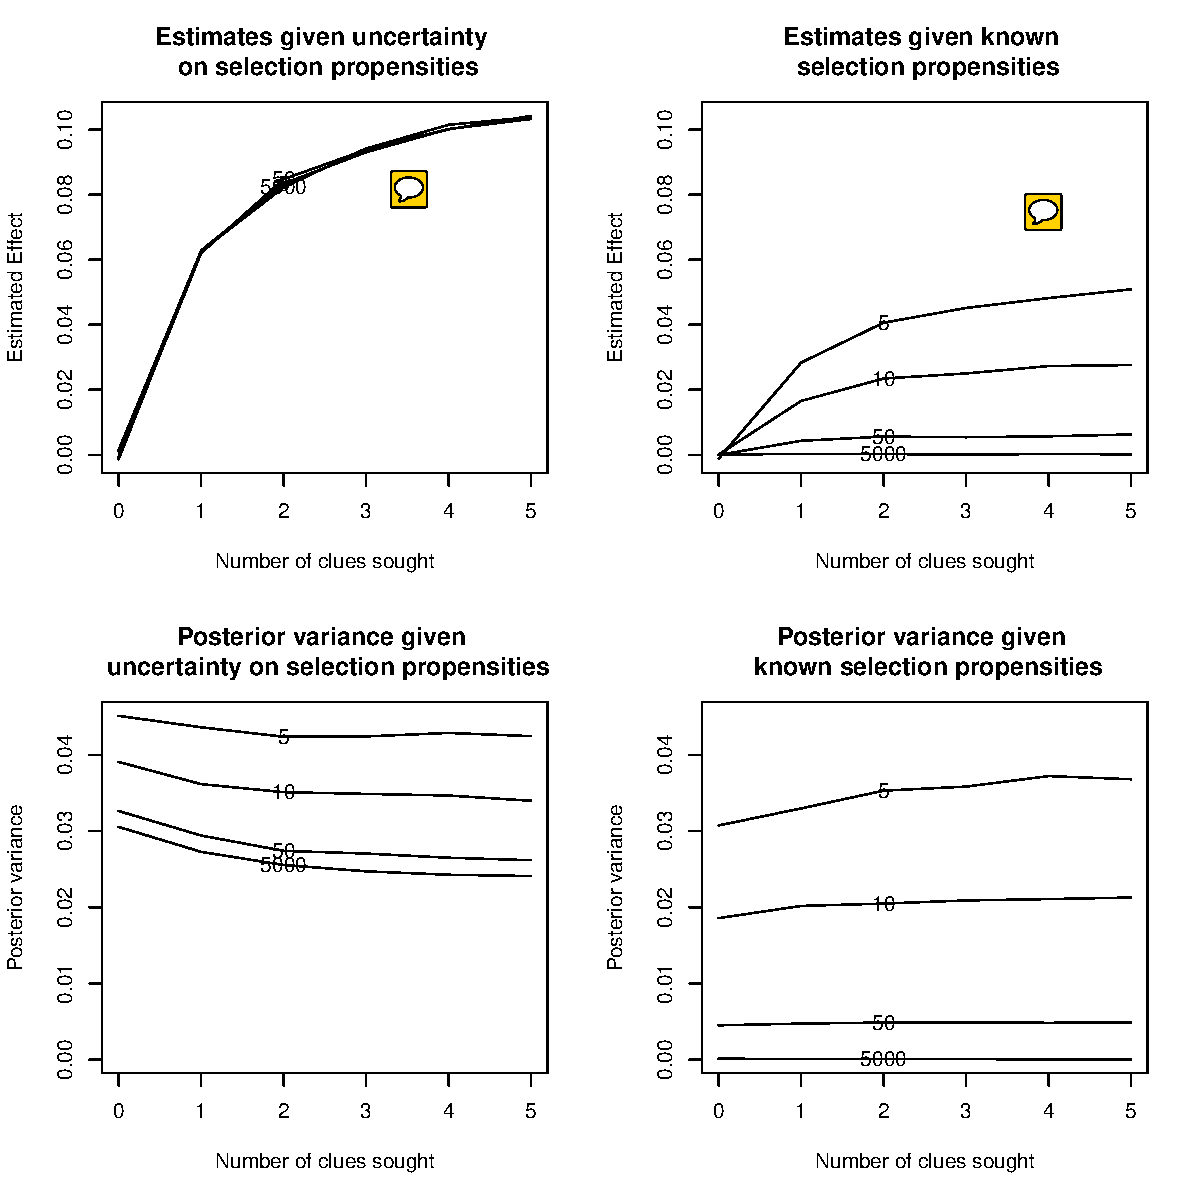
\includegraphics[width=\textwidth]{Figures/Ns.pdf}
\caption{{Figure shows posterior estimates of the average treatment effect and posterior variances given a situation with 5, 10, 50, or 5000 observations in each cell of an $X,Y$ table and given collection of data on $0 - 5$ cases in the $X=Y=1$ cell, all of which provide evidence from a doubly decisive clue in favor of causal effects.}}
\label{morn}
\end{figure}

\hypertarget{evaluating-strategies}{%
\section{Evaluating strategies}\label{evaluating-strategies}}

As a metric of the returns from different research strategies we calculate the \emph{expected} inaccuracy in the estimation of the average treatment effect, as given in equation \ref{Loss}.
\begin{equation}
\mathcal{L}=\mathbb{E}_\theta(\mathbb{E}_{\mathcal{D}|\theta}(\tau(\theta)-\hat{\tau}(\mathcal{D}))^2) 
\label{Loss}
\end{equation}

where \(\tau(\theta)\) is the value of \(\lambda_b-\lambda_a\) (the average treatment effect) given \(\theta\), and \(\hat{\tau}(\mathcal{D})\) is the \emph{estimate} of this treatment effect (the mean posterior value) that is generated following some realization of data \(\mathcal{D}\). Thus, if some \(\theta\) characterized the true state of the world, then \(\mathbb{E}_{\mathcal{D}|\theta}(\tau^\theta-\hat{\tau})^2\) is the expected error in estimation of the causal effect given different realizations of the data, \(\mathcal{D}\), that could obtain in this state of the world. \(\mathcal{L}\) is then the expected value of these errors given prior beliefs over possible values of \(\theta\).

Note that, while we focus on errors on estimated average causal effects, similar exercises could assess how cross- and within-case observations distinctively contribute to other estimands \textbar{} including the causal explanations for individual cases and the validity of causal theories \textbar{} as well as to learning about inferential assumptions themselves (assignment and clue probabilities).
For all simulations, prior distributions are drawn with parameters as described in the Supplementary Materials (\S \ref{AppSimNotes}, Table \ref{tab:sims}). Priors on the type distribution are drawn from a Dirichlet distribution; priors for each of the \(\pi\) and \(\phi\) values are drawn independently from Beta distributions. We note that, while by construction priors on each parameter are independent, this will not generally be the case for posterior distributions. In most cases we simulate the prior distribution using 5200 draws of each parameter. For most experiments we then systematically vary the prior distribution for one parameter of the research situation between two extreme positions. We then calculate the expected posterior from each possible data realization and, in turn, the expected loss in estimates of treatment effects for a range of levels of investment in qualitative and quantitative evidence.

A few further features of the experiments below are worth noting. First, our illustrations focus on learning about population-level causal effects; however, the model can yield results about the benefits of alternative research designs for estimating a wide range of other quantities of interest, such as case-specific causal explanations or clue probabilities. Second, while we focus on the search for a \emph{single} clue in each case, the analysis can be extended to the case of an arbitrarily large set of clues. Third, in many of these experiments, the probative values are set at doubly decisive levels for all \(\phi\) parameters, and thus focus on the very optimistic case of maximally informative process tracing. Fourth, we illustrate tradeoffs at low levels of \(n\), but the model can be employed to make choices for arbitrarily large numbers of cases. Finally, we note that some results may be sensitive to the choice of priors. The results below should thus be understood as an illustration of the utility of the BIQQ framework for guiding research choices, rather than as a set of more general prescriptive design rules.

\hypertarget{varieties}{%
\section{Varieties of mixing}\label{varieties}}

What are the marginal gains from additional pieces of correlational and process-tracing evidence for the accuracy of causal estimates? Figure \ref{morn} displays the results, plotting the errors associated with different mixes of correlational and process data. Each dot represents a single possible research design, with the \(x\)-axis charting the total the number of cases examined. For all cases, \(X\) and \(Y\) data are collected. The shading of the dots in each column then represents the proportion of cases for which process-tracing is also carried out. An unshaded dot is a design in which \emph{only} correlational data has been collected for all cases; a black dot is a design in which the process-tracing clue is sought in \emph{all} cases; and shades of grey, as they darken, indicate process tracing for increasing shares of cases. For \(n\leq 4\) we report results for all designs; for \(n>4\) we report only results when within case information is sought for all, half, or none of the cases.

We see first from the graph that, as one would expect, moving from lower-\(n\) to higher-\(n\) designs reduces the expected error of estimates. Further, both adding a correlational case and doing process tracing on an additional case improve accuracy. The figure also suggests that there are diminishing marginal returns to both types of data: in particular the grey point reflecting 50\% process tracing is generally well below the mid point of the white and black dots, and converges toward the black dot (100\% process tracing) as sample size increases. Other, less obvious results also emerge, including:

\begin{itemize}
\item **Qualitative and quantitative data can act as partial substitutes for assessing causal effects**. We see, in the smaller sample sizes, that the marginal gains from adding an extra case are lower when there is more within-case information on existing cases. Similarly, the marginal gains from gathering more within-case information are lower when there are more correlational cases (for example adding one case study when $n=1$ has about the same effect as adding 8 cases studies when $n=16$). 
\item **The *relative* marginal gains from going wider and going deeper vary with the study design**. Suppose that the costs of gathering $X,Y$ data and gathering clue data were the same per case. Suppose further that we have an $n$ of 2 and only correlational data. Then, for the case illustrated in Figure \ref{morn}, if we have additional resources to invest, it is better to gather $K$-type data for 1 of these cases than to add another case with $X,Y$ data only. However, at this point, the tradeoff shifts. If we now have a choice of gathering $K$-type data on the second case (moving to the black dot) or adding a third case (resulting in $n=4,m=1$), the latter strategy now results in an error rate at least as low as the former. %
% Sometimes it is better to go deeper than wider. For example an $n$=3 (or $n$=2) study with process tracing on one case produces greater accuracy than a purely correlational $n=4$ (or $n=3$) study. 
\item **Optimal strategies might involve going deep in a subsample of cases only**. Suppose again that the costs for gathering $X,Y$ data and gathering $K$-type data were the same and, now, that researchers can gather four pieces of data of any type. The results in Figure \ref{morn} suggest that, for the priors chosen here, gathering $X,Y$ data on 3 cases and $K$-type data on one produces more accurate estimates than either going maximally wide (gathering $X,Y$ data on four cases) and at least as accurate an estimate as going maximally deep (gathering $X,Y,K$ data on 2 cases).
 %At the margins and once one has done some process tracing, the results suggest that it is better to invest in additional $X,Y$ data *without* clues than to seek to do process tracing for all cases on which one has $X,Y$ data.

\end{itemize}

\begin{figure}[h!]
\centering
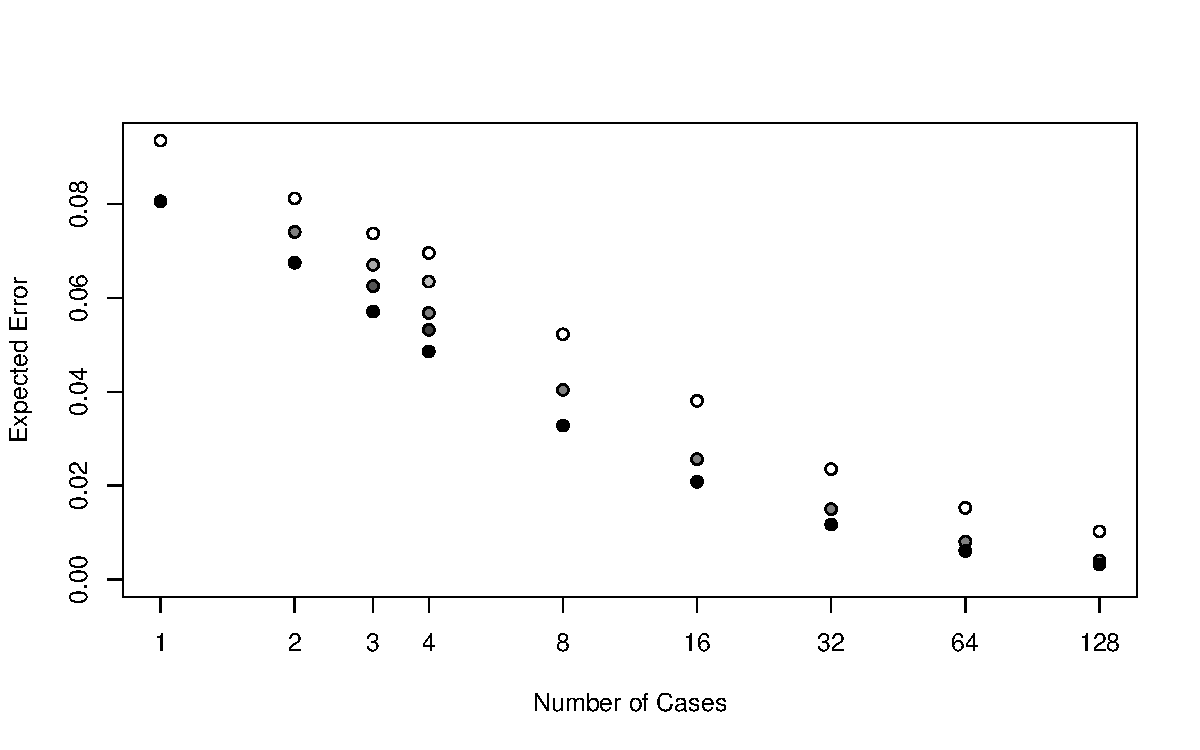
\includegraphics[width=\textwidth]{Figures/m_or_n.pdf}
\caption{{Expected errors in the estimation of average treatment effects for designs in which $X, Y$, data is sought in $n$ studies (horizontal axis) and clue data is sought within $m$ of these. The shading of dots indicates the proportion of cases for which within-case data is sought (white = none; black = all). For small sample sizes ($n \in \{1,2,3,4\}$) we show results for all designs ($m \in \{1,2,\dots, n\})$. For larger sample sizes, we show only designs with clues sought in 0, half, and all cases.}}
\label{morn}
\end{figure}

\subsection{Designs in Context}

More generally, we would expect that the optimal level of mixing depends on the context\textbar{}on features of the research situation that affect the problem and available tools of inference. In the next subsections, we report results from experiments in which we vary the researcher's priors about (a.) the probative value of clues, (b.) heterogeneity of treatment effects (c.) uncertainty regarding assignment processes, and (d.) uncertainty regarding the probative value of clues. In all cases we report the expected loss for the design in question, as given in Equation \ref{Loss}. \%

\subsubsection{Probative value of clues}

If clues have no probative value\textbar{} in the sense that priors over \(\phi_{jx}\) do not depend on type, \(j\), then gathering data on clues does not affect inference. Probative value does not get picked up during analysis, it must be imported. Less clear, however, is the extent to which gains in inference depend on the degree of probative value, defined here as in Section \ref{PTintro} (see footnote \ref{fnPV}). Our simulation evidence from full BIQQ estimation (Figure \ref{experiments}) suggests that in some ranges at least the gains are also convex, that is \emph{increasingly} more is learned as the gaps between pairs such as \(\phi_{b1}\) and \(\phi_{d1}\) increases. The top left panel of Figure \ref{experiments} shows an example of these convex gains, showing expected losses for settings where there is not probative value, where all tests are doubly decisive, and a case half way between these extremes.

\begin{figure}[h!]
\centering
\includegraphics[width=\textwidth]{Figures/experiments.pdf}
\caption{Figure shows the expected error in mean posterior estimates of average treatment effects for different designs. In these graphs the horizontal axis denotes some feature of the research setting (captured in priors); the white and black circles represent errors from designs in which within case information is sought for no and all cases, respectively; the numbers marked in the circles indicate the number of data points in the study design.}
\label{experiments}
\end{figure}

\subsubsection{Effect Heterogeneity}

We might expect that the optimal research design for estimating average treatment effects would depend on how \emph{heterogeneous} the true causal effects are in the population. If we believe that effects are strongly homogeneous, then confidence that one case is affected by treatment provides a great deal of information about population treatment effects. However, if effects are believed to be highly heterogeneous, then knowing that one case is affected by treatment provides less information regarding effects on different cases.

Heterogeneity can be conceptualized in different ways. Here we define heterogeneity as increasing in the amount of \emph{variance} in causal effects across cases in the population. In the binary environment, for any \(\tau \in [0,1]\), maximum effect heterogeneity is obtained when \(\lambda_a=(1-\tau)/2\) and \(\lambda_b=(1+\tau)/2\): i.e., when all cases have either a positive or negative treatment effect, with no destined or chronic cases. For a positive treatment effect, maximum homogeneity occurs when \(a=0, b=\tau\), with the remaining share \(1-\tau\) consisting of types \(c\) and \(d\).\footnote{For negative treatment effects, homogeneity is maximized with \(\lambda_b=0\).} There are two very different ways to have an average treatment effect of 0: there may be no treatment effect for any case (maximal homogeneity), or there is a positive effect for half the cases and a negative effect for the other half (maximal heterogeneity).\\
\%Here there is no variance in causal effects across cases.

Using this conceptualization of heterogeneity, our simulation results confirm that higher heterogeneity increases the marginal value of going `'wide'' rather than `'deep.'' At low levels of heterogeneity, there are considerable gains to collecting clues on cases at a given sample size; but the gains to process tracing diminish and then disappear as heterogeneity rises (see Supplementary Materials, \S\ref{AppE2}).

\%Above, why is homogeneity defined only for a=0? Also, I don't understand why maximal homogeneity isn't a, b, c, or d = 1. How does learning about one case tell you so much more about the population under the definition of homogeneity above?
\% that's homogeneity of type, but not of treatment effect; e.g.~all c is no more homogeneous than half a and half b. the second het analysis looks at a case like this though

\subsubsection{Uncertainty Regarding Assignment Processes}

Here we examine the implications of uncertainty over treatment assignment (confounding).

Any differences in assignment probabilities that are \emph{known} are built into our priors in a Bayesian setting and do not produce biases (just as known confounds can be controlled for in a standard regression model). However, \emph{uncertainty} about assignment processes still generates higher variance in posterior estimates \citep[see][]{GerGreKap04}. \% where variance of the prior distribution of bias is infinite. In this case, they show that it is optimal to place resources in strategies that have no uncertainty around sources of bias---such as in experimental data collection rather than observational data collection. Similarly, authors in the process tracing tradition have argued that a key feature of process tracing is its capacity to detect reverse causation, omitted variables, and other confounding processes (e.g., \citep{Lieberman2005nested}.
In the BIQQ framework, however, clues provide discriminatory leverage on case types that is \emph{independent} of assignment probabilities: with strong probative value, \(b\) and \(d\) type treated units can be told apart thus eliminating the identification problem that certainty over assignment processes helps to solve.\\
\%How does the level of uncertainty about assignment affect the optimal design mix?
In our simulations (bottom left panel of Figure \ref{experiments}), we find that greater uncertainty over assignment processes indeed results in greater errors for correlational analysis \textbar{} most obviously for higher \(n\). However, for the parameter space we examine (and given strong assumptions on the probative value of clues), uncertainty about assignment does not reduce accuracy for mixed methods analysis. \%Mixed methods analysis, that is, appears more robust to violations of the ignorability assumption.
(See Supplementary Materials, \S\ref{AppE3}.)

\subsubsection{Uncertainty regarding the probative value of clues}

\%The critical assumption for drawing inferences from clues is that researchers know the likelihood of clues being present as a function of type: that is, that we know the likelihood with which a given piece of process-based evidence should be observed if a given causal effect is truly present. This is clearly a strong assumption. \%, dependent on identifying both the right theoretical logic for each causal effect and the ways in which that logic would make itself observable in within-case data.
\%In this sense, process tracing rests on a set of assumptions that may be just as uncertain as the assumption of particular (conditional) assignment probabilities made in observational quantitative research.
As with assignment probabilities, researchers may be uncertain regarding the probative value of clues for discriminating between types. How much does this uncertainty matter for the relative gains to qualitative evidence?

Surprisingly, our simulations suggest that uncertainty over the probative values of clues is unimportant for expected errors (see Supplementary Materials, \S\ref{AppE4}). Our experiment fixes the expected probative value of a clue and allows for variance around that expected value. Informally, we are thus comparing a situation in which one believes that a clue has moderate probative value to one in which one believes that it may have strong probative value or it may have none at all.

To be clear, this analysis does \emph{not} imply that there is no penalty to being \emph{wrong} about the probative value of clues. \%If a researcher is convinced that a clue has more probative value than it actually has, then the researcher will draw the wrong inferences.
The result suggests rather, that having more, rather than less, \emph{uncertainty} about that probative value may be relatively inconsequential for the choice of research strategy.

\hypertarget{AppSimNotes}{%
\section{Notes on Simulations}\label{AppSimNotes}}

Here we provide statistical details and some further interpretation for the paper's simulations assessing the benefits of different designs conditional on different priors regarding the probative value of clues, the heterogeneity of causal effects, uncertainty regarding assignment probabilities, and uncertainty regarding the probative value of clues. Table \ref{tab:sims} provides details on all parameters used in simulations and Table \ref{simdetails} provides detail on the number of runs, iterations, and related information used in the estimation.

\hypertarget{AppE1}{%
\subsection{Probative values}\label{AppE1}}

For these simulations we simultaneously vary the probative value for tests for all \(X,Y\) combinations. Specifically, we vary the differences between \(\phi_{b0}\) and \(\phi_{c0}\) (for \(X=Y=0\) cases), between \(\phi_{a0}\) and \(\phi_{d0}\) (for \(X=0, Y=1\) cases); between \(\phi_{a1}\) and \(\phi_{c1}\) (for \(X=1, Y=0\) cases); and between \(\phi_{b1}\) and \(\phi_{d1}\) (for \(X=Y=1\) cases). For each \(X,Y\) combination, we compare the relevant \(\phi\) pairs across values of \((.5,.5)\) (no probative value), \((.25,.75)\) (middling probative value) and \((0.01,0.99)\) (strong probative value). Using the definition of probative value (PV) we provide (Section \ref{PTintro}, see footnote \ref{fnPV}), these correspond to cases with probative value of 0, .5, and close to 1 respectively.

\hypertarget{AppE2}{%
\subsection{Effect heterogeneity}\label{AppE2}}

We note that heterogeneity makes going `'wide'' relatively more beneficial for two reasons. First, when all cases are affected either positively or negatively, all of the information needed to identify types is provided by information on \(X\) and \(Y\). If \(X=Y\) then a case was (or could have been) positively affected; if \(X \ne Y\) then a case was (or could have been) negatively affected. In this extreme case of maximal heterogeneity, causal process information provides no additional inferential gains. Where there is high homogeneity, on the other hand, the core difficulty is distinguishing \(a\) and \(b\) types, from \(c\) and \(d\) types. Then, the information contained in clues may provide greater benefits (see Table \ref{FP}). Second, the more heterogeneous effects are across cases, the less we learn about \emph{population-level} causal effects by getting an individual case right. Thus, again, we would expect greater relative gains to more extensive analysis as heterogeneity increases.

\hypertarget{AppE3}{%
\subsection{Uncertainty about assignment processes}\label{AppE3}}

Note that in our binary setup, infinite bias cannot arise, and the harm done by uncertainty over selection processes can be more moderate. In this set of simulations, the expected value of \(\pi_j\) is fixed at \(0.5\) and we vary the variance in \(\pi_j\) between 0 and a maximum of 0.289.

\hypertarget{AppE4}{%
\subsection{Uncertainty regarding the probative value of clues}\label{AppE4}}

In this experiment, the expected probability that a clue will be observed is set to 0.75 if one hypothesis is right, and 0.25 if the alternative hypothesis is correct. The simulations vary from a situation in which those probabilities are known with certainty (uncertainty low) to a situation in which the researcher admits the possibility of many possible values of \(\phi\) (uncertainty set to its maximum of 0.25). Uncertainty is simultaneously varied for all pairs of \(\phi\) values (see \S\ref{AppE1}). The displayed results suggest that uncertainty about the probative value of clues plays little role in the assessment of optimal strategies. Fixing the penumbra of uncertainty around a given expected \(\phi\) value allows for the possibility that the clue may have weak probative value, but also that it may have exceptionally strong probative value. The effects of these possibilities appear to wash out when we update beliefs about causal effects upon observation of the clue (or its absence).

\hypertarget{details-on-simulation-experiments}{%
\subsection{Details on simulation experiments}\label{details-on-simulation-experiments}}

\begin{longtable}[]{@{}ccclcccclcclccrc@{}}
\caption{\label{tab:sims}Simulation parameters. Each column details parameters used to generate prior distributions for one of the simulations below. The prior distribution for the full parameter vector is formed from independent draws from Beta distributions for all probabilities and the Dirichlet distribution for shares. Note that the mean and standard deviation parameterization we provide for Beta distributions can be mapped directly to the more standard \(\alpha, \beta\) parameterization}\tabularnewline
\toprule
\begin{minipage}[b]{0.03\columnwidth}\centering
\(\theta\)\strut
\end{minipage} & \begin{minipage}[b]{0.03\columnwidth}\centering
Dist\strut
\end{minipage} & \begin{minipage}[b]{0.03\columnwidth}\centering
arg\strut
\end{minipage} & \begin{minipage}[b]{0.03\columnwidth}\raggedright
1: m or n\textbackslash{}\strut
\end{minipage} & \begin{minipage}[b]{0.05\columnwidth}\centering
2: Probative Value\\
Low\strut
\end{minipage} & \begin{minipage}[b]{0.03\columnwidth}\centering
\(\rightarrow\)\strut
\end{minipage} & \begin{minipage}[b]{0.03\columnwidth}\centering
High\strut
\end{minipage} & \begin{minipage}[b]{0.06\columnwidth}\centering
3: Effect Heterogeneity\\
Low\strut
\end{minipage} & \begin{minipage}[b]{0.03\columnwidth}\raggedright
\(\rightarrow\)\strut
\end{minipage} & \begin{minipage}[b]{0.03\columnwidth}\centering
High\strut
\end{minipage} & \begin{minipage}[b]{0.07\columnwidth}\centering
4: Assignment Uncertainty\\
Low\strut
\end{minipage} & \begin{minipage}[b]{0.03\columnwidth}\raggedright
\(\rightarrow\)\strut
\end{minipage} & \begin{minipage}[b]{0.04\columnwidth}\centering
High\strut
\end{minipage} & \begin{minipage}[b]{0.05\columnwidth}\centering
5: Clue Uncertainty\\
Low\strut
\end{minipage} & \begin{minipage}[b]{0.03\columnwidth}\raggedleft
\(\rightarrow\)\strut
\end{minipage} & \begin{minipage}[b]{0.03\columnwidth}\centering
High\strut
\end{minipage}\tabularnewline
\midrule
\endfirsthead
\toprule
\begin{minipage}[b]{0.03\columnwidth}\centering
\(\theta\)\strut
\end{minipage} & \begin{minipage}[b]{0.03\columnwidth}\centering
Dist\strut
\end{minipage} & \begin{minipage}[b]{0.03\columnwidth}\centering
arg\strut
\end{minipage} & \begin{minipage}[b]{0.03\columnwidth}\raggedright
1: m or n\textbackslash{}\strut
\end{minipage} & \begin{minipage}[b]{0.05\columnwidth}\centering
2: Probative Value\\
Low\strut
\end{minipage} & \begin{minipage}[b]{0.03\columnwidth}\centering
\(\rightarrow\)\strut
\end{minipage} & \begin{minipage}[b]{0.03\columnwidth}\centering
High\strut
\end{minipage} & \begin{minipage}[b]{0.06\columnwidth}\centering
3: Effect Heterogeneity\\
Low\strut
\end{minipage} & \begin{minipage}[b]{0.03\columnwidth}\raggedright
\(\rightarrow\)\strut
\end{minipage} & \begin{minipage}[b]{0.03\columnwidth}\centering
High\strut
\end{minipage} & \begin{minipage}[b]{0.07\columnwidth}\centering
4: Assignment Uncertainty\\
Low\strut
\end{minipage} & \begin{minipage}[b]{0.03\columnwidth}\raggedright
\(\rightarrow\)\strut
\end{minipage} & \begin{minipage}[b]{0.04\columnwidth}\centering
High\strut
\end{minipage} & \begin{minipage}[b]{0.05\columnwidth}\centering
5: Clue Uncertainty\\
Low\strut
\end{minipage} & \begin{minipage}[b]{0.03\columnwidth}\raggedleft
\(\rightarrow\)\strut
\end{minipage} & \begin{minipage}[b]{0.03\columnwidth}\centering
High\strut
\end{minipage}\tabularnewline
\midrule
\endhead
\begin{minipage}[t]{0.03\columnwidth}\centering
\(\lambda_a\)\strut
\end{minipage} & \begin{minipage}[t]{0.03\columnwidth}\centering
Dirichlet\strut
\end{minipage} & \begin{minipage}[t]{0.03\columnwidth}\centering
\(\alpha_a\)\strut
\end{minipage} & \begin{minipage}[t]{0.03\columnwidth}\raggedright
1\\
\strut
\end{minipage} & \begin{minipage}[t]{0.05\columnwidth}\centering
0.20\\
\strut
\end{minipage} & \begin{minipage}[t]{0.03\columnwidth}\centering
\(\rightarrow\)\strut
\end{minipage} & \begin{minipage}[t]{0.03\columnwidth}\centering
0.20\\
\strut
\end{minipage} & \begin{minipage}[t]{0.06\columnwidth}\centering
0.10\\
\strut
\end{minipage} & \begin{minipage}[t]{0.03\columnwidth}\raggedright
\(\rightarrow\)\strut
\end{minipage} & \begin{minipage}[t]{0.03\columnwidth}\centering
\textbf{2.00}\strut
\end{minipage} & \begin{minipage}[t]{0.07\columnwidth}\centering
1\\
\strut
\end{minipage} & \begin{minipage}[t]{0.03\columnwidth}\raggedright
\(\rightarrow\)\strut
\end{minipage} & \begin{minipage}[t]{0.04\columnwidth}\centering
1\\
\strut
\end{minipage} & \begin{minipage}[t]{0.05\columnwidth}\centering
1\\
\strut
\end{minipage} & \begin{minipage}[t]{0.03\columnwidth}\raggedleft
\(\rightarrow\)\strut
\end{minipage} & \begin{minipage}[t]{0.03\columnwidth}\centering
1\\
\strut
\end{minipage}\tabularnewline
\begin{minipage}[t]{0.03\columnwidth}\centering
\(\lambda_b\)\strut
\end{minipage} & \begin{minipage}[t]{0.03\columnwidth}\centering
\strut
\end{minipage} & \begin{minipage}[t]{0.03\columnwidth}\centering
\(\alpha_b\)\strut
\end{minipage} & \begin{minipage}[t]{0.03\columnwidth}\raggedright
1\\
\strut
\end{minipage} & \begin{minipage}[t]{0.05\columnwidth}\centering
0.20\\
\strut
\end{minipage} & \begin{minipage}[t]{0.03\columnwidth}\centering
\(\rightarrow\)\strut
\end{minipage} & \begin{minipage}[t]{0.03\columnwidth}\centering
0.20\\
\strut
\end{minipage} & \begin{minipage}[t]{0.06\columnwidth}\centering
02.10\\
\strut
\end{minipage} & \begin{minipage}[t]{0.03\columnwidth}\raggedright
\(\rightarrow\)\strut
\end{minipage} & \begin{minipage}[t]{0.03\columnwidth}\centering
\textbf{4.00}\strut
\end{minipage} & \begin{minipage}[t]{0.07\columnwidth}\centering
1\\
\strut
\end{minipage} & \begin{minipage}[t]{0.03\columnwidth}\raggedright
\(\rightarrow\)\strut
\end{minipage} & \begin{minipage}[t]{0.04\columnwidth}\centering
1\\
\strut
\end{minipage} & \begin{minipage}[t]{0.05\columnwidth}\centering
1\\
\strut
\end{minipage} & \begin{minipage}[t]{0.03\columnwidth}\raggedleft
\(\rightarrow\)\strut
\end{minipage} & \begin{minipage}[t]{0.03\columnwidth}\centering
1\\
\strut
\end{minipage}\tabularnewline
\begin{minipage}[t]{0.03\columnwidth}\centering
\(\lambda_c\)\strut
\end{minipage} & \begin{minipage}[t]{0.03\columnwidth}\centering
\strut
\end{minipage} & \begin{minipage}[t]{0.03\columnwidth}\centering
\(\alpha_c\)\strut
\end{minipage} & \begin{minipage}[t]{0.03\columnwidth}\raggedright
1\\
\strut
\end{minipage} & \begin{minipage}[t]{0.05\columnwidth}\centering
0.20\\
\strut
\end{minipage} & \begin{minipage}[t]{0.03\columnwidth}\centering
\(\rightarrow\)\strut
\end{minipage} & \begin{minipage}[t]{0.03\columnwidth}\centering
0.20\\
\strut
\end{minipage} & \begin{minipage}[t]{0.06\columnwidth}\centering
02.00\\
\strut
\end{minipage} & \begin{minipage}[t]{0.03\columnwidth}\raggedright
\(\rightarrow\)\strut
\end{minipage} & \begin{minipage}[t]{0.03\columnwidth}\centering
\textbf{0.10}\strut
\end{minipage} & \begin{minipage}[t]{0.07\columnwidth}\centering
1\\
\strut
\end{minipage} & \begin{minipage}[t]{0.03\columnwidth}\raggedright
\(\rightarrow\)\strut
\end{minipage} & \begin{minipage}[t]{0.04\columnwidth}\centering
1\\
\strut
\end{minipage} & \begin{minipage}[t]{0.05\columnwidth}\centering
1\\
\strut
\end{minipage} & \begin{minipage}[t]{0.03\columnwidth}\raggedleft
\(\rightarrow\)\strut
\end{minipage} & \begin{minipage}[t]{0.03\columnwidth}\centering
1\\
\strut
\end{minipage}\tabularnewline
\begin{minipage}[t]{0.03\columnwidth}\centering
\(\lambda_d\)\strut
\end{minipage} & \begin{minipage}[t]{0.03\columnwidth}\centering
\strut
\end{minipage} & \begin{minipage}[t]{0.03\columnwidth}\centering
\(\alpha_d\)\strut
\end{minipage} & \begin{minipage}[t]{0.03\columnwidth}\raggedright
1\\
\strut
\end{minipage} & \begin{minipage}[t]{0.05\columnwidth}\centering
0.20\\
\strut
\end{minipage} & \begin{minipage}[t]{0.03\columnwidth}\centering
\(\rightarrow\)\strut
\end{minipage} & \begin{minipage}[t]{0.03\columnwidth}\centering
0.20\\
\strut
\end{minipage} & \begin{minipage}[t]{0.06\columnwidth}\centering
02.00\\
\strut
\end{minipage} & \begin{minipage}[t]{0.03\columnwidth}\raggedright
\(\rightarrow\)\strut
\end{minipage} & \begin{minipage}[t]{0.03\columnwidth}\centering
\textbf{0.10}\strut
\end{minipage} & \begin{minipage}[t]{0.07\columnwidth}\centering
1\\
\strut
\end{minipage} & \begin{minipage}[t]{0.03\columnwidth}\raggedright
\(\rightarrow\)\strut
\end{minipage} & \begin{minipage}[t]{0.04\columnwidth}\centering
1\\
\strut
\end{minipage} & \begin{minipage}[t]{0.05\columnwidth}\centering
1\\
\strut
\end{minipage} & \begin{minipage}[t]{0.03\columnwidth}\raggedleft
\(\rightarrow\)\strut
\end{minipage} & \begin{minipage}[t]{0.03\columnwidth}\centering
1\\
\strut
\end{minipage}\tabularnewline
\begin{minipage}[t]{0.03\columnwidth}\centering
\(\pi_a\)\strut
\end{minipage} & \begin{minipage}[t]{0.03\columnwidth}\centering
Beta\strut
\end{minipage} & \begin{minipage}[t]{0.03\columnwidth}\centering
\(\mu\)
\(\sigma\)\strut
\end{minipage} & \begin{minipage}[t]{0.03\columnwidth}\raggedright
0.50\\
0.10\\
\strut
\end{minipage} & \begin{minipage}[t]{0.05\columnwidth}\centering
0.50\\
0.10\\
\strut
\end{minipage} & \begin{minipage}[t]{0.03\columnwidth}\centering
\(\rightarrow\)
\(\rightarrow\)\strut
\end{minipage} & \begin{minipage}[t]{0.03\columnwidth}\centering
0.50\\
0.10\\
\strut
\end{minipage} & \begin{minipage}[t]{0.06\columnwidth}\centering
0.50\\
0.10\\
\strut
\end{minipage} & \begin{minipage}[t]{0.03\columnwidth}\raggedright
\(\rightarrow\)
\(\rightarrow\)\strut
\end{minipage} & \begin{minipage}[t]{0.03\columnwidth}\centering
0.50\\
0.10\\
\strut
\end{minipage} & \begin{minipage}[t]{0.07\columnwidth}\centering
0.50\\
0.01\\
\strut
\end{minipage} & \begin{minipage}[t]{0.03\columnwidth}\raggedright
\(\rightarrow\)
\(\rightarrow\)\strut
\end{minipage} & \begin{minipage}[t]{0.04\columnwidth}\centering
0.50\\
\textbf{0.289}\strut
\end{minipage} & \begin{minipage}[t]{0.05\columnwidth}\centering
0.50\\
0.10\\
\strut
\end{minipage} & \begin{minipage}[t]{0.03\columnwidth}\raggedleft
\(\rightarrow\)
\(\rightarrow\)\strut
\end{minipage} & \begin{minipage}[t]{0.03\columnwidth}\centering
0.50\\
0.10\\
\strut
\end{minipage}\tabularnewline
\begin{minipage}[t]{0.03\columnwidth}\centering
\(\pi_b\)\strut
\end{minipage} & \begin{minipage}[t]{0.03\columnwidth}\centering
Beta\strut
\end{minipage} & \begin{minipage}[t]{0.03\columnwidth}\centering
\(\mu\)
\(\sigma\)\strut
\end{minipage} & \begin{minipage}[t]{0.03\columnwidth}\raggedright
0.50\\
0.10\\
\strut
\end{minipage} & \begin{minipage}[t]{0.05\columnwidth}\centering
0.50\\
0.10\\
\strut
\end{minipage} & \begin{minipage}[t]{0.03\columnwidth}\centering
\(\rightarrow\)
\(\rightarrow\)\strut
\end{minipage} & \begin{minipage}[t]{0.03\columnwidth}\centering
0.50\\
0.10\\
\strut
\end{minipage} & \begin{minipage}[t]{0.06\columnwidth}\centering
0.50\\
0.10\\
\strut
\end{minipage} & \begin{minipage}[t]{0.03\columnwidth}\raggedright
\(\rightarrow\)
\(\rightarrow\)\strut
\end{minipage} & \begin{minipage}[t]{0.03\columnwidth}\centering
0.50\\
0.10\\
\strut
\end{minipage} & \begin{minipage}[t]{0.07\columnwidth}\centering
0.50\\
0.01\\
\strut
\end{minipage} & \begin{minipage}[t]{0.03\columnwidth}\raggedright
\(\rightarrow\)
\(\rightarrow\)\strut
\end{minipage} & \begin{minipage}[t]{0.04\columnwidth}\centering
0.50\\
\textbf{0.289}\strut
\end{minipage} & \begin{minipage}[t]{0.05\columnwidth}\centering
0.50\\
0.10\\
\strut
\end{minipage} & \begin{minipage}[t]{0.03\columnwidth}\raggedleft
\(\rightarrow\)
\(\rightarrow\)\strut
\end{minipage} & \begin{minipage}[t]{0.03\columnwidth}\centering
0.50\\
0.10\\
\strut
\end{minipage}\tabularnewline
\begin{minipage}[t]{0.03\columnwidth}\centering
\(\pi_c\)\strut
\end{minipage} & \begin{minipage}[t]{0.03\columnwidth}\centering
Beta\strut
\end{minipage} & \begin{minipage}[t]{0.03\columnwidth}\centering
\(\mu\)
\(\sigma\)\strut
\end{minipage} & \begin{minipage}[t]{0.03\columnwidth}\raggedright
0.50\\
0.10\\
\strut
\end{minipage} & \begin{minipage}[t]{0.05\columnwidth}\centering
0.50\\
0.10\\
\strut
\end{minipage} & \begin{minipage}[t]{0.03\columnwidth}\centering
\(\rightarrow\)
\(\rightarrow\)\strut
\end{minipage} & \begin{minipage}[t]{0.03\columnwidth}\centering
0.50\\
0.10\\
\strut
\end{minipage} & \begin{minipage}[t]{0.06\columnwidth}\centering
0.50\\
0.10\\
\strut
\end{minipage} & \begin{minipage}[t]{0.03\columnwidth}\raggedright
\(\rightarrow\)
\(\rightarrow\)\strut
\end{minipage} & \begin{minipage}[t]{0.03\columnwidth}\centering
0.50\\
0.10\\
\strut
\end{minipage} & \begin{minipage}[t]{0.07\columnwidth}\centering
0.50\\
0.01\\
\strut
\end{minipage} & \begin{minipage}[t]{0.03\columnwidth}\raggedright
\(\rightarrow\)
\(\rightarrow\)\strut
\end{minipage} & \begin{minipage}[t]{0.04\columnwidth}\centering
0.50\\
\textbf{0.289}\strut
\end{minipage} & \begin{minipage}[t]{0.05\columnwidth}\centering
0.50\\
0.10\\
\strut
\end{minipage} & \begin{minipage}[t]{0.03\columnwidth}\raggedleft
\(\rightarrow\)
\(\rightarrow\)\strut
\end{minipage} & \begin{minipage}[t]{0.03\columnwidth}\centering
0.50\\
0.10\\
\strut
\end{minipage}\tabularnewline
\begin{minipage}[t]{0.03\columnwidth}\centering
\(\pi_d\)\strut
\end{minipage} & \begin{minipage}[t]{0.03\columnwidth}\centering
Beta\strut
\end{minipage} & \begin{minipage}[t]{0.03\columnwidth}\centering
\(\mu\)
\(\sigma\)\strut
\end{minipage} & \begin{minipage}[t]{0.03\columnwidth}\raggedright
0.50\\
0.10\\
\strut
\end{minipage} & \begin{minipage}[t]{0.05\columnwidth}\centering
0.50\\
0.10\\
\strut
\end{minipage} & \begin{minipage}[t]{0.03\columnwidth}\centering
\(\rightarrow\)
\(\rightarrow\)\strut
\end{minipage} & \begin{minipage}[t]{0.03\columnwidth}\centering
0.50\\
0.10\\
\strut
\end{minipage} & \begin{minipage}[t]{0.06\columnwidth}\centering
0.50\\
0.10\\
\strut
\end{minipage} & \begin{minipage}[t]{0.03\columnwidth}\raggedright
\(\rightarrow\)
\(\rightarrow\)\strut
\end{minipage} & \begin{minipage}[t]{0.03\columnwidth}\centering
0.50\\
0.10\\
\strut
\end{minipage} & \begin{minipage}[t]{0.07\columnwidth}\centering
0.50\\
0.01\\
\strut
\end{minipage} & \begin{minipage}[t]{0.03\columnwidth}\raggedright
\(\rightarrow\)
\(\rightarrow\)\strut
\end{minipage} & \begin{minipage}[t]{0.04\columnwidth}\centering
0.50\\
\textbf{0.289}\strut
\end{minipage} & \begin{minipage}[t]{0.05\columnwidth}\centering
0.50\\
0.10\\
\strut
\end{minipage} & \begin{minipage}[t]{0.03\columnwidth}\raggedleft
\(\rightarrow\)
\(\rightarrow\)\strut
\end{minipage} & \begin{minipage}[t]{0.03\columnwidth}\centering
0.50\\
0.10\\
\strut
\end{minipage}\tabularnewline
\begin{minipage}[t]{0.03\columnwidth}\centering
\(\phi_{a0}\)\strut
\end{minipage} & \begin{minipage}[t]{0.03\columnwidth}\centering
Beta\strut
\end{minipage} & \begin{minipage}[t]{0.03\columnwidth}\centering
\(\mu\)
\(\sigma\)\strut
\end{minipage} & \begin{minipage}[t]{0.03\columnwidth}\raggedright
0.01\\
0.01\\
\strut
\end{minipage} & \begin{minipage}[t]{0.05\columnwidth}\centering
0.50\\
0.01\\
\strut
\end{minipage} & \begin{minipage}[t]{0.03\columnwidth}\centering
\(\rightarrow\)
\(\rightarrow\)\strut
\end{minipage} & \begin{minipage}[t]{0.03\columnwidth}\centering
\textbf{0.01}
0.01\\
\strut
\end{minipage} & \begin{minipage}[t]{0.06\columnwidth}\centering
0.01\\
0.01\\
\strut
\end{minipage} & \begin{minipage}[t]{0.03\columnwidth}\raggedright
\(\rightarrow\)
\(\rightarrow\)\strut
\end{minipage} & \begin{minipage}[t]{0.03\columnwidth}\centering
0.01\\
0.01\\
\strut
\end{minipage} & \begin{minipage}[t]{0.07\columnwidth}\centering
0.01\\
0.01\\
\strut
\end{minipage} & \begin{minipage}[t]{0.03\columnwidth}\raggedright
\(\rightarrow\)
\(\rightarrow\)\strut
\end{minipage} & \begin{minipage}[t]{0.04\columnwidth}\centering
0.01\\
0.01\\
\strut
\end{minipage} & \begin{minipage}[t]{0.05\columnwidth}\centering
0.01\\
0.001\\
\strut
\end{minipage} & \begin{minipage}[t]{0.03\columnwidth}\raggedleft
\(\rightarrow\)
\(\rightarrow\)\strut
\end{minipage} & \begin{minipage}[t]{0.03\columnwidth}\centering
0.25\\
\textbf{0.25}\strut
\end{minipage}\tabularnewline
\begin{minipage}[t]{0.03\columnwidth}\centering
\(\phi_{a1}\)\strut
\end{minipage} & \begin{minipage}[t]{0.03\columnwidth}\centering
Beta\strut
\end{minipage} & \begin{minipage}[t]{0.03\columnwidth}\centering
\(\mu\)
\(\sigma\)\strut
\end{minipage} & \begin{minipage}[t]{0.03\columnwidth}\raggedright
0.99\\
0.01\\
\strut
\end{minipage} & \begin{minipage}[t]{0.05\columnwidth}\centering
0.50\\
0.01\\
\strut
\end{minipage} & \begin{minipage}[t]{0.03\columnwidth}\centering
\(\rightarrow\)
\(\rightarrow\)\strut
\end{minipage} & \begin{minipage}[t]{0.03\columnwidth}\centering
\textbf{0.99}
0.01\\
\strut
\end{minipage} & \begin{minipage}[t]{0.06\columnwidth}\centering
0.99\\
0.01\\
\strut
\end{minipage} & \begin{minipage}[t]{0.03\columnwidth}\raggedright
\(\rightarrow\)
\(\rightarrow\)\strut
\end{minipage} & \begin{minipage}[t]{0.03\columnwidth}\centering
0.99\\
0.01\\
\strut
\end{minipage} & \begin{minipage}[t]{0.07\columnwidth}\centering
0.99\\
0.01\\
\strut
\end{minipage} & \begin{minipage}[t]{0.03\columnwidth}\raggedright
\(\rightarrow\)
\(\rightarrow\)\strut
\end{minipage} & \begin{minipage}[t]{0.04\columnwidth}\centering
0.99\\
0.01\\
\strut
\end{minipage} & \begin{minipage}[t]{0.05\columnwidth}\centering
0.75\\
0.001\\
\strut
\end{minipage} & \begin{minipage}[t]{0.03\columnwidth}\raggedleft
\(\rightarrow\)
\(\rightarrow\)\strut
\end{minipage} & \begin{minipage}[t]{0.03\columnwidth}\centering
0.75\\
\textbf{0.25}\strut
\end{minipage}\tabularnewline
\begin{minipage}[t]{0.03\columnwidth}\centering
\(\phi_{b0}\)\strut
\end{minipage} & \begin{minipage}[t]{0.03\columnwidth}\centering
Beta\strut
\end{minipage} & \begin{minipage}[t]{0.03\columnwidth}\centering
\(\mu\)
\(\sigma\)\strut
\end{minipage} & \begin{minipage}[t]{0.03\columnwidth}\raggedright
0.01\\
0.01\\
\strut
\end{minipage} & \begin{minipage}[t]{0.05\columnwidth}\centering
0.50\\
0.01\\
\strut
\end{minipage} & \begin{minipage}[t]{0.03\columnwidth}\centering
\(\rightarrow\)
\(\rightarrow\)\strut
\end{minipage} & \begin{minipage}[t]{0.03\columnwidth}\centering
\textbf{0.01}
0.01\\
\strut
\end{minipage} & \begin{minipage}[t]{0.06\columnwidth}\centering
0.01\\
0.01\\
\strut
\end{minipage} & \begin{minipage}[t]{0.03\columnwidth}\raggedright
\(\rightarrow\)
\(\rightarrow\)\strut
\end{minipage} & \begin{minipage}[t]{0.03\columnwidth}\centering
0.01\\
0.01\\
\strut
\end{minipage} & \begin{minipage}[t]{0.07\columnwidth}\centering
0.01\\
0.01\\
\strut
\end{minipage} & \begin{minipage}[t]{0.03\columnwidth}\raggedright
\(\rightarrow\)
\(\rightarrow\)\strut
\end{minipage} & \begin{minipage}[t]{0.04\columnwidth}\centering
0.01\\
0.01\\
\strut
\end{minipage} & \begin{minipage}[t]{0.05\columnwidth}\centering
0.25\\
0.001\\
\strut
\end{minipage} & \begin{minipage}[t]{0.03\columnwidth}\raggedleft
\(\rightarrow\)
\(\rightarrow\)\strut
\end{minipage} & \begin{minipage}[t]{0.03\columnwidth}\centering
0.25\\
\textbf{0.25}\strut
\end{minipage}\tabularnewline
\begin{minipage}[t]{0.03\columnwidth}\centering
\(\phi_{b1}\)\strut
\end{minipage} & \begin{minipage}[t]{0.03\columnwidth}\centering
Beta\strut
\end{minipage} & \begin{minipage}[t]{0.03\columnwidth}\centering
\(\mu\)
\(\sigma\)\strut
\end{minipage} & \begin{minipage}[t]{0.03\columnwidth}\raggedright
0.99\\
0.01\\
\strut
\end{minipage} & \begin{minipage}[t]{0.05\columnwidth}\centering
0.50\\
0.01\\
\strut
\end{minipage} & \begin{minipage}[t]{0.03\columnwidth}\centering
\(\rightarrow\)
\(\rightarrow\)\strut
\end{minipage} & \begin{minipage}[t]{0.03\columnwidth}\centering
\textbf{0.99}
0.01\\
\strut
\end{minipage} & \begin{minipage}[t]{0.06\columnwidth}\centering
0.99\\
0.01\\
\strut
\end{minipage} & \begin{minipage}[t]{0.03\columnwidth}\raggedright
\(\rightarrow\)
\(\rightarrow\)\strut
\end{minipage} & \begin{minipage}[t]{0.03\columnwidth}\centering
0.99\\
0.01\\
\strut
\end{minipage} & \begin{minipage}[t]{0.07\columnwidth}\centering
0.99\\
0.01\\
\strut
\end{minipage} & \begin{minipage}[t]{0.03\columnwidth}\raggedright
\(\rightarrow\)
\(\rightarrow\)\strut
\end{minipage} & \begin{minipage}[t]{0.04\columnwidth}\centering
0.99\\
0.01\\
\strut
\end{minipage} & \begin{minipage}[t]{0.05\columnwidth}\centering
0.75\\
0.001\\
\strut
\end{minipage} & \begin{minipage}[t]{0.03\columnwidth}\raggedleft
\(\rightarrow\)
\(\rightarrow\)\strut
\end{minipage} & \begin{minipage}[t]{0.03\columnwidth}\centering
0.75\\
\textbf{0.25}\strut
\end{minipage}\tabularnewline
\begin{minipage}[t]{0.03\columnwidth}\centering
\(\phi_{c0}\)\strut
\end{minipage} & \begin{minipage}[t]{0.03\columnwidth}\centering
Beta\strut
\end{minipage} & \begin{minipage}[t]{0.03\columnwidth}\centering
\(\mu\)
\(\sigma\)\strut
\end{minipage} & \begin{minipage}[t]{0.03\columnwidth}\raggedright
0.99\\
0.01\\
\strut
\end{minipage} & \begin{minipage}[t]{0.05\columnwidth}\centering
0.50\\
0.01\\
\strut
\end{minipage} & \begin{minipage}[t]{0.03\columnwidth}\centering
\(\rightarrow\)
\(\rightarrow\)\strut
\end{minipage} & \begin{minipage}[t]{0.03\columnwidth}\centering
\textbf{0.99}
0.01\\
\strut
\end{minipage} & \begin{minipage}[t]{0.06\columnwidth}\centering
0.99\\
0.01\\
\strut
\end{minipage} & \begin{minipage}[t]{0.03\columnwidth}\raggedright
\(\rightarrow\)
\(\rightarrow\)\strut
\end{minipage} & \begin{minipage}[t]{0.03\columnwidth}\centering
0.99\\
0.01\\
\strut
\end{minipage} & \begin{minipage}[t]{0.07\columnwidth}\centering
0.99\\
0.01\\
\strut
\end{minipage} & \begin{minipage}[t]{0.03\columnwidth}\raggedright
\(\rightarrow\)
\(\rightarrow\)\strut
\end{minipage} & \begin{minipage}[t]{0.04\columnwidth}\centering
0.99\\
0.01\\
\strut
\end{minipage} & \begin{minipage}[t]{0.05\columnwidth}\centering
0.75\\
0.001\\
\strut
\end{minipage} & \begin{minipage}[t]{0.03\columnwidth}\raggedleft
\(\rightarrow\)
\(\rightarrow\)\strut
\end{minipage} & \begin{minipage}[t]{0.03\columnwidth}\centering
0.75\\
\textbf{0.25}\strut
\end{minipage}\tabularnewline
\begin{minipage}[t]{0.03\columnwidth}\centering
\(\phi_{c1}\)\strut
\end{minipage} & \begin{minipage}[t]{0.03\columnwidth}\centering
Beta\strut
\end{minipage} & \begin{minipage}[t]{0.03\columnwidth}\centering
\(\mu\)
\(\sigma\)\strut
\end{minipage} & \begin{minipage}[t]{0.03\columnwidth}\raggedright
0.01\\
0.01\\
\strut
\end{minipage} & \begin{minipage}[t]{0.05\columnwidth}\centering
0.50\\
0.01\\
\strut
\end{minipage} & \begin{minipage}[t]{0.03\columnwidth}\centering
\(\rightarrow\)
\(\rightarrow\)\strut
\end{minipage} & \begin{minipage}[t]{0.03\columnwidth}\centering
\textbf{0.01}
0.01\\
\strut
\end{minipage} & \begin{minipage}[t]{0.06\columnwidth}\centering
0.01\\
0.01\\
\strut
\end{minipage} & \begin{minipage}[t]{0.03\columnwidth}\raggedright
\(\rightarrow\)
\(\rightarrow\)\strut
\end{minipage} & \begin{minipage}[t]{0.03\columnwidth}\centering
0.01\\
0.01\\
\strut
\end{minipage} & \begin{minipage}[t]{0.07\columnwidth}\centering
0.01\\
0.01\\
\strut
\end{minipage} & \begin{minipage}[t]{0.03\columnwidth}\raggedright
\(\rightarrow\)
\(\rightarrow\)\strut
\end{minipage} & \begin{minipage}[t]{0.04\columnwidth}\centering
0.01\\
0.01\\
\strut
\end{minipage} & \begin{minipage}[t]{0.05\columnwidth}\centering
0.25\\
0.001\\
\strut
\end{minipage} & \begin{minipage}[t]{0.03\columnwidth}\raggedleft
\(\rightarrow\)
\(\rightarrow\)\strut
\end{minipage} & \begin{minipage}[t]{0.03\columnwidth}\centering
0.25\\
\textbf{0.25}\strut
\end{minipage}\tabularnewline
\begin{minipage}[t]{0.03\columnwidth}\centering
\(\phi_{d0}\)\strut
\end{minipage} & \begin{minipage}[t]{0.03\columnwidth}\centering
Beta\strut
\end{minipage} & \begin{minipage}[t]{0.03\columnwidth}\centering
\(\mu\)
\(\sigma\)\strut
\end{minipage} & \begin{minipage}[t]{0.03\columnwidth}\raggedright
0.99\\
0.01\\
\strut
\end{minipage} & \begin{minipage}[t]{0.05\columnwidth}\centering
0.50\\
0.01\\
\strut
\end{minipage} & \begin{minipage}[t]{0.03\columnwidth}\centering
\(\rightarrow\)
\(\rightarrow\)\strut
\end{minipage} & \begin{minipage}[t]{0.03\columnwidth}\centering
\textbf{0.99}
0.01\\
\strut
\end{minipage} & \begin{minipage}[t]{0.06\columnwidth}\centering
0.99\\
0.01\\
\strut
\end{minipage} & \begin{minipage}[t]{0.03\columnwidth}\raggedright
\(\rightarrow\)
\(\rightarrow\)\strut
\end{minipage} & \begin{minipage}[t]{0.03\columnwidth}\centering
0.99\\
0.01\\
\strut
\end{minipage} & \begin{minipage}[t]{0.07\columnwidth}\centering
0.99\\
0.01\\
\strut
\end{minipage} & \begin{minipage}[t]{0.03\columnwidth}\raggedright
\(\rightarrow\)
\(\rightarrow\)\strut
\end{minipage} & \begin{minipage}[t]{0.04\columnwidth}\centering
0.99\\
0.01\\
\strut
\end{minipage} & \begin{minipage}[t]{0.05\columnwidth}\centering
0.75\\
0.001\\
\strut
\end{minipage} & \begin{minipage}[t]{0.03\columnwidth}\raggedleft
\(\rightarrow\)
\(\rightarrow\)\strut
\end{minipage} & \begin{minipage}[t]{0.03\columnwidth}\centering
0.75\\
\textbf{0.25}\strut
\end{minipage}\tabularnewline
\begin{minipage}[t]{0.03\columnwidth}\centering
\(\phi_{d1}\)\strut
\end{minipage} & \begin{minipage}[t]{0.03\columnwidth}\centering
Beta\strut
\end{minipage} & \begin{minipage}[t]{0.03\columnwidth}\centering
\(\mu\)
\(\sigma\)\strut
\end{minipage} & \begin{minipage}[t]{0.03\columnwidth}\raggedright
0.01\\
0.01\\
\strut
\end{minipage} & \begin{minipage}[t]{0.05\columnwidth}\centering
0.50\\
0.01\\
\strut
\end{minipage} & \begin{minipage}[t]{0.03\columnwidth}\centering
\(\rightarrow\)
\(\rightarrow\)\strut
\end{minipage} & \begin{minipage}[t]{0.03\columnwidth}\centering
\textbf{0.01}
0.01\\
\strut
\end{minipage} & \begin{minipage}[t]{0.06\columnwidth}\centering
0.01\\
0.01\\
\strut
\end{minipage} & \begin{minipage}[t]{0.03\columnwidth}\raggedright
\(\rightarrow\)
\(\rightarrow\)\strut
\end{minipage} & \begin{minipage}[t]{0.03\columnwidth}\centering
0.01\\
0.01\\
\strut
\end{minipage} & \begin{minipage}[t]{0.07\columnwidth}\centering
0.01\\
0.01\\
\strut
\end{minipage} & \begin{minipage}[t]{0.03\columnwidth}\raggedright
\(\rightarrow\)
\(\rightarrow\)\strut
\end{minipage} & \begin{minipage}[t]{0.04\columnwidth}\centering
0.01\\
0.01\\
\strut
\end{minipage} & \begin{minipage}[t]{0.05\columnwidth}\centering
0.25\\
0.001\\
\strut
\end{minipage} & \begin{minipage}[t]{0.03\columnwidth}\raggedleft
\(\rightarrow\)
\(\rightarrow\)\strut
\end{minipage} & \begin{minipage}[t]{0.03\columnwidth}\centering
0.25\\
\textbf{0.25}\strut
\end{minipage}\tabularnewline
\bottomrule
\end{longtable}

\newpage

\normalsize

\begin{table}
\footnotesize
\centering
\begin{tabular}{lccp{8cm}} 
                        & $j$ steps             & $k$ sims                  &                   \\ 
Experiment              & per exp.              & per step                  & Comments                  \\ \hline
**1:**
Varying $N$ or $m$      & 29                    & 5,200                             & The 5,200 $k$ simulations for each $\theta_j$ were split into 26 runs of 200 $k$ sims, and then
                                                                                      compiled through averaging. \\
                                                                                     
&&&                 Datapoints at N=3 and N=4 were added using 14,200 $k$ simulations. \\\\
**2:**
Probative Value         & 30                    & 5,200                             & The 5,200 $k$ simulations for each $\theta_j$ were split into 26 batches of 200 $k$ sims, and then
                                                                                      compiled through averaging.  \\ \\
**3:**
Effect Heterogeneity    & 30                    & 5,200                             & The 5,200 $k$ simulations for each $\theta_j$ were split into 26 batches of 200 $k$ sims, and then
                                                                                      compiled through averaging.  \\ \\
**4:**
Assignment Uncertainty  & 30                    & 5,200                             & The 5,200 $k$ simulations for each $\theta_j$ were split into 26 batches of 200 $k$ sims, and then
                                                                                      compiled through averaging.  \\ \\
**5:**
Clue Uncertainty        & 30                    & 10,200                            & The 10,200 $k$ simulations for each $\theta_j$ were split into 26 batches of 200 $k$ sims and 
                                                                                      10 batches of 500, then
                                                                                      compiled through averaging.  \\
\end{tabular}
\caption{\footnotesize *Note:* 
Each experiment takes $j$ steps through different values of $\theta$. At each $\theta_j$, the data is simulated $k$ times. For each simulation,   
a call is made to the Stan model and HMC (Hamiltonian Monte Carlo) sampling is used
to approximate the posterior distribution. 
In each such call to Stan, we run 4 chains with 6000 iterations, and 
1000 warmup draws.}
\label{simdetails}
\end{table}

\hypertarget{caseselection}{%
\chapter{Case selection as a Decision Problem}\label{caseselection}}

\begin{center}\rule{0.5\linewidth}{\linethickness}\end{center}

With a causal model in hand, together with priors over parameters, you can assess in advance what conclusions you will draw from different observations and assess what kinds of observations are most worth seeking. We draw out the implicaitons of this idea for case selection.

\begin{center}\rule{0.5\linewidth}{\linethickness}\end{center}

A critical decision for scholars employing mixed methods is to determine which cases are most valuable for within-case analysis.

A host of different strategies have been proposed for selecting cases for in-depth study based on the observed values of \(X\), \(Y\) data. Perhaps the most common strategy is to select cases in which \(X=1\) and \(Y=1\) and look to see whether in fact \(X\) caused \(Y\) in the case in question (using some more or less formal strategy for inferring causality from within-case evidence). But many other strategies have been proposed, including strategies to select cases ``on the regression line'' or, for some purposes, cases ``off the regression line'' (e.g., \citet{Lieberman2005nested}). Some scholars suggest ensuring variation in \(X\) (most prominently, \citet{king1994designing}), while others have proposed various kinds of matching strategies. Some have pointed to the advantages of random sampling of cases, either stratified or unstratified by values on \(X\) or \(Y\) (\citet{FL2008}, \citet{HerronQuinn}).

Which cases you should choose will likely depend on the purposes to which you want to put them.

A matching strategy for instance---selecting cases that are comparable on many features but that differ on \(X\)---replicates at a small scale the kind of inference done by matching estimators with large-\(n\) data. The strategy emphasize the inferences to be made from \(X,Y\) variation rather than inferences drawn specifically from within case information beyond what is available in the measurement of \(X\) and \(Y\). (Citations needed.)

Other treatments seek to use qualitative information to check assumptions made in \(X, Y\) analysis: for example, is the measurement of \(X\) and \(Y\) reliable in critical cases? (Citations needed) For such questions with limited resources, it might make sense to focus on cases for which validation plausibly makes a difference to the \(X,Y\) inferences: for example influential cases that have unusually extreme values on \(X\) and \(Y\).\^{}{[}Note: We can say more about why these would be good choices from a Bayesian perspective, based on the idea that measurement is more likely to be wrong in such cases and shifting them to more typical values would make a big difference.{]} Similar arguments are made for checking assumptions on selection processes, though we consider this a more complex desideratum since this requires making case level causal inferences and not simply measurement claims.

A third purpose is to use a case to generate alternative or richer theories of causal processes, as in Lieberman's ``model-building'' mode of ``nested analysis'' (\citet{Lieberman2005nested}). Here it may be cases off the regression line that are of interest.

Weller and Barnes (CITE article) on case selection focus on (a) X/Y relations and (b) whether the cases are useful for hypothesis generation.

In what follows, we focus on a simpler goal: given existing \(X, Y\) data for a set of cases and a given clue (or set of clues) that we can go looking for in the intensive analysis of some subset of these cases, for which cases would process tracing yield the greatest learning about the population-level causal effect of \(X\) on \(Y\)?

The basic insight of this chapter is simple enough: the optimal strategy for case selection for a model-based analysis can be determined by the model and the query, just as we saw for the optimal clue-selection strategy in Chapter \ref{Clues}. Using this strategy yields guidance that is consistent with some common advice but at odds with other advice. The main principles that emerge from the analysis can be summarized as:

\begin{itemize}
\tightlist
\item
  sample from \(X\) and \(Y\) values in proportion to their occurrence in the population,
\item
  go where the probative value is, and
\item
  invest in collections of cases that provide complementary learning.
\end{itemize}

Beyond these general principles, other patterns are more complex and thus more difficult to neatly summarize. The most general message of this chapter is about the general approach: that is, that we can use a causal model to tell us what kinds of cases are likely to yield the greatest learning, given the model and a strategy of inference. We provide a tool for researchers to undertake this analysis, at least for simple problems with \(X, Y, K\) data.

For the general intuition, recall that the probative value of a process-tracing test hinges on the difference in clue likelihoods associated with the alternative hypotheses in play for a given case. Recall that for different values of \(X\) and \(Y\) cell, we want to use process tracing to help us distinguish between two specific types that are consistent with the \(X, Y\) pattern. Which types are in question varies across \(X,Y\) combinations. Table \ref{FP} illustrates.

\begin{table}[h!]
\centering
\begin{tabular}{c|cc}
           &        $Y=0$ &        $Y=1$ \\ \hline
       $X=0$ &     $b$ or $c$ &     $a$ or $d$ \\
       $X=1$ &     $a$ or $c$ &     $b$ or $d$ \\
\end{tabular}  
\caption{The ambiguity about types in each $X, Y$ cell.}
\label{FP} 
\end{table}

Thus, in the \(X=0, Y-0\) cell, what would be most useful is a clue that has high probative value in distinguishing between an untreated (\(X=0\)) \(b\) type and and an untreated \(c\) type. For a case in the \(X=1, Y=0\) cell, on the other hand, what matters is how well the clue can discriminate between treated (\(X=1\)) \(a\) and \(d\) types. In our notation, it is the difference in \(phi_{jx}\) values for that indicates these cell-specific degrees of leverage.

To illustrate, consider a situation in which for a given clue we have \(\phi_{b1}\)=0.5\footnote{The probability of observing the clue for a \(b\) type (positive causal effect) case with \(X=1\).}; \(\phi_{d1}\)=0.5 \footnote{The probability of observing the clue for a \(d\) type (zero causal effect, \(Y\) fixed at 1) case with \(X=1\).}; \(\phi_{b0}\)=0.5\^{}\footnote{The probability of observing the clue for a \(b\) type (positive causal effect) case with \(X=0\).}; and \(\phi_{c0}\)=0.1\footnote{The probability of observing the clue for a \(c\) type (zero causal effect, \(Y\) fixed at 0) case with \(X=0\).}. In this situation, searching for the clue in \(X=Y=1\) cases will yield no leverage since the clue does not discriminate between the two types (\(b\) and \(d\)) that need to be distinguished given \(X=Y=1\). Here there is no additional learning about \(\lambda_b\) that can be gained from looking for the clue. In contrast, \(X=0, Y=0\) cases will be informative since the clue is much better at distinguishing between \(b\) and \(c\) types---the two types in contention for this kind of case. Thus, although process tracing here does not provide information on the prevalence of positive causal effects (\(b\) types) for an \(X=Y=1\) case, it does provide information when \(X=Y=0\).

While it is common practice for mixed-method researchers to perform their process tracing ``on the regression line,'' the BIQQ framework suggests that the gains to process tracing for different \(X\) and \(Y\) values in fact depend on the particular constellations of \(\phi\) values for the potentially available clues. More generally, the framework allows one to assess the expected gains from any given case-selection strategy \emph{ex ante} once priors have been specified.

\hypertarget{explorations}{%
\section{Explorations}\label{explorations}}

Most closely related to our analysis in this chapter is the contribution of \citet{HerronQuinn}, who build on \citet{SeawrightGerring2008}. While Seawright and Gerring provide a taxonomy of approaches to case selection, they do not provide a strategy for assessing the relative merits of these different approaches. As we do, \citet{HerronQuinn} focus on a situation with binary \(X,Y\) data and assess the gains from learning about causal type in a set of cases (interestingly in their treatment causal type, \(Z_i\) is called a confounder rather than being an estimand of direct interest; in our setup, confounding as normally understood arises because of different probabilities of different causal types of being assigned to ``treatment'', or an \(X=1\) value). \citet{HerronQuinn} assume that in any given case selected for analysis a qualitative researcher is able to infer the causal type perfectly.

Our setup differs from that in \citet{HerronQuinn} in a few ways. \citet{HerronQuinn} paramaterize differently, though this difference is not important.\footnote{\citet{HerronQuinn} have a parameter \(\theta\) that governs the distribution of data over \(X\) and \(Y\) and then, conditional on \(X,Y\) values, a set of parameters \(\psi_{xy}\) that describe the probability of a case's being of a given causal type. We take both \(\theta\) and \(\psi_{xy}\) to derive from the fundamental distribution of causal types and assignment probabilities. Thus, for example, \(\psi_{00}\) from \citet{HerronQuinn} corresponds to \(\frac{(1-\pi_b)\lambda_b}{(1-\pi_b)\lambda_b + (1-\pi_c)\lambda_c}\) in our notation. The difference in paramaterization does have implications for interpretations of the priors. For example flat priors over \(\theta\) and \(\psi\) implies a tighter distribution that a uniform prior over the causal types. In fact \citet{HerronQuinn} use priors with greater variance than uniform in any event.} Perhaps the most important difference between our analysis and that in \citet{HerronQuinn} is that we connect the inference strategy to process-tracing approaches. Whereas \citet{HerronQuinn} assume that causal types can be read directly, we assume that these are inferred \emph{imperfectly} from clues. As in our baseline model, our ability to make inferences for causal types can differ by type and as a function of \(X\). And, as in the baseline model, not only can we have uncertainty about the probative value of clues, but researchers can learn about the probative value of clues by examining cases.

Here we assume that the case selection decision is made after observing the \(XY\) distribution and we explore a range of different possible contingency tables. In \citet{HerronQuinn} the distribution from which the contingency tables are drawn is fixed, though set to exhibit an expected observed difference in means (though not necessarily a true treatment effect) of 0.2. They assume large \(XY\) data sets (with 10,000) units and case selection strategies ranging from 1 to 20 cases.

Another important difference, is that in many of their analyses, \citet{HerronQuinn} take the perspective of an outside analyst who knows the true treatment effect; they then assess the expected bias generated by a research strategy over the possible data realizations. We, instead, take the perspective of a researcher who has \emph{beliefs} about the true treatment effect that correspond to their priors, and for whom there is therefore no \emph{expected} bias. This has consequences also for the assessment of expected posterior variance, as in our analyses the expectation of the variance is taken with respect to the researcher's beliefs about the world, rather than being made conditional on some specific world (ATE). We think that this setup is addressed to the question that a researcher must answer when deciding on a strategy: given what they know now, what will produce the greatest reduction in uncertainty (the lowest expected posterior variance)?

Finally, we proceed somewhat differently in our identification of strategies from Herron and Quinn: rather than pre-specifying particular sets of strategies (operationalizations of those identified by \citet{SeawrightGerring2008}) and evaluating them, we define a strategy as the particular distribution over \(XY\) cells to be examined and proceed to examine \emph{every possible strategy} given a choice of a certain number of cases in which to conduct process tracing. We thus let the clusters of strategies---those strategies that perform similarly---emerge from the analysis rather than being privileged by past conceptualizations of case-selection strategies.

Despite these various differences, our results will agree in key ways with those in \citet{HerronQuinn}.

\hypertarget{procedure}{%
\subsection{Procedure}\label{procedure}}

To illustrate the procedure, consider a researcher who observes six data points. Two cases lie in each of the on-diagonal cells of an \(X,Y\) table, those where \(X=Y\), and one case lies in each of the off-diagonal cells (where \(X \neq Y\)). Suppose that the researcher is considering gathering process-tracing clues on 3 cases. She has many different strategies she might pursue and each of these can give rise to different possible data and thus to different possible conclusions. Let's say that she starts with no knowledge about (flat priors over) the distribution of causal types in the population, assumes similar assignment propensities for all types (no confounding), and believes that the clues she is going to look for are all doubly decisive (either seeing the clue or not seeing the clue, when she looks for it, will fully identify the case's type).

Suppose, now, that she is choosing between two strategies:

A. Select two \(X=Y=1\) cases and one \(X=Y=0\) case for investigation. She is thus choosing here cases ``on the regression line'' generated by the \(X,Y\) data pattern.

B. Take one case from each of the diagonal cells and one from the off-diagonal \(X=1, Y=0\) cell

From which strategy should she expect to learn more about the average, population-level causal effect of \(X\) on \(Y\), given her prior beliefs? We answer the question by considering each data pattern that she might see given a strategy and then calculating (a) the probability with which she expects to see such an outcome, given her priors (or more accurately, given her posterior after observing the \(XY\) pattern only), and (b) the uncertainty (posterior variance) that she would have upon seeing that pattern. We then calculate the expected variance of the strategy by considering all possible data patterns that could emerge from that strategy. We ignore the fact that in principle the subjective probability of observing one pattern is correlated with the subjective probability of observing another pattern.\footnote{For example, a researcher may be uncertain regarding \(\phi_b\); if it is high then the probability of observing any profile of outcomes with many clues observed is higher than if \(\phi_b\) is low; this introduces a correlation between outcomes that have similar clue observations. However only one of these patterns will be observed in fact. NOTE ON RISK-NEUTRALITY HERE?}

Tables 11.1 and 11.2 present the results of our comparison of the researcher's two strategies. Table 11.1 examines strategy A, while Table 11.2 examines strategy B. In each table, the lefthand column lists all possible realizations of clue data that might be found under the strategy in question. In the notation that we use here, each place in the four-digit sequence refers to one cell in the 2-by-2 table implied by a binary \(X\) and binary \(Y\) variable. The ordering is:

\begin{itemize}
\tightlist
\item
  \(X=Y=0\)
\item
  \(X=0, Y=1\)
\item
  \(X=1, Y=0\)
\item
  \(X=Y=1\)
\end{itemize}

As an easy mnemonic, the outside digits are ``on-the-diagonal'' (on the regression line consistent with a positive causal effect); the inside digits are off-the-diagonal. Thus, for instance, the sequence \(1001\) means that we have seen the clue in two on-the-diagonal cases: an \(X=Y=0\) case and a \(X=Y=1\) case. The sequence 0200 means that we have seen the clue in two cases in the \(X=0, Y=1\) cell.

In each row, we see information about one possible clue pattern that we could potentially observe under the strategy. The second column indicates the probability that this clue pattern will arise, given the researcher's priors. The final column then indicates the uncertainty---the posterior variance---that we would be left with given the information provided by that clue pattern. In the ``All'' row, we have averaged across the posterior variances for all clue patterns, weighting each clue pattern by its probability of occurring.

REDO BIQQ LOSSES WITH NEW FUNCTIONS

REDO

\begin{table}[t]

\caption{\label{tab:unnamed-chunk-86}Inferences from  strategy A: one cell from one on-the-regression-line cell; two from the other. Each row shows possible clue patterns one might see from a given strategy, where, for example 1000 means that a clue is indeed observed for an X=0, Y=0 case.}
\centering
\begin{tabular}{r}
\hline
redo\\
\hline
0\\
\hline
\end{tabular}
\end{table}

\begin{table}[t]

\caption{\label{tab:unnamed-chunk-86}Inferences from  strategy B: one case from each of the diagonal cells and one from the off-diagonal $X=1, Y=0$ cell. Each row shows possible clue patterns one might see from a given strategy, where, for example 1000 means that a clue is indeed observed for an X=0, Y=0 case.}
\centering
\begin{tabular}{r}
\hline
redo\\
\hline
0\\
\hline
\end{tabular}
\end{table}

In this example, we see that the researcher would expect to be better off---in the sense of having less posterior uncertainty---by focusing her process-tracing efforts where a greater share of the population of cases lies: on the regression line. Taking one observation in each of three cells has her devoting much of her effort to a case that is relatively unrepresentative of the population she wishes to learn about.

In the experiments that follow, we implement this kind of simulation for all possible clue strategies---for a fixed number of clues sought---and report the expected posterior variance.

\hypertarget{experiments}{%
\section{Experiments}\label{experiments}}

In all of the graphs, we start with 16 ``quantitative'' cases: cases for which we have observed an \(X\) and a \(Y\) value. We are then choosing some subset of these cases for process tracing. Within each group of nine graphs, we are sampling a fixed number of cases for process tracing: 1 case in the first set, 2 cases in the second set, 3 cases in the third set, and 4 cases in the final set. We treat process tracing in a case as the search for one clue in that case, though this ``one clue'' could be conceived of as a collection of clues that jointly have a given probative value.

Within each set of graphs, we see how different case selection strategies fare as we vary two features of the research situation. Moving down the rows of graphs, we vary the distribution of the 16 cases over an \(XY\) table. In the first row, the 16 cases are spread evenly across the 4 \(X,Y\) cells; in the second row, \(X\) and \(Y\) are positively correlated; in the third row, \(Y=1\) is observed only in cases with \(X=1\) (i.e., the \(X=0, Y=1\) cell is empty).

Moving across the columns of graphs, we vary the probative value of the clue that we are looking for in the process tracing. What is changing is for what kind of a case---in terms of its \(X,Y\) values---the clue is most probative (i.e., doubly decisive). Where the clue is doubly decisive, finding the clue present or finding it absent both nail down the type of the case. Wherever the clue is not doubly decisive, it is assumed to be a ``hoop test'' for an \(a\) type (in the \(X=1, Y=0\) and \(X=0, Y=1\) cells) and for a \(b\) type (in the \(X=0, Y=1\) cells). This means that \emph{not} finding the clue rules out the case's being an \(a\) or a \(b\) type in the relevant cells; thus, the clue is still informative, but less so than if it were doubly decisive. In the first column, the clue is doubly decisive for all kinds of cases. In the second column, the clue is doubly decisive only for \(X=1\) cases, and a hoop test otherwise. In the third column, the clue is doubly decisive only for \(Y=1\) cases, and a hoop test otherwise. And in the final column, the clue is doubly decisive only ``on the regression line'' consistent with a positive effect, and a hoop test otherwise.

Each case selection strategy is indicated on each graph using the same four-digit pattern that we used to indicate data realizations in the example above. Throughout, what we seek to estimate is the average causal effect of \(X\) on \(Y\) (or \(\lambda_b-\lambda_a\)). The strategy's vertical placement on the graph indicates the ``loss'', i.e., expected posterior uncertainty, associated with the strategy. Thus, a lower placement indicates greater learning. Around each dot, we also provide 90 percent simulation error bars, though these are hidden by the dots themselves when the simulation error is very small, as it is in most cases.

In all simulations, we assume that there is no confounding, and we start (before seeing the \(X, Y\) pattern) with flat priors over the distribution of causal types in the population.

In the graphs with more than one process tracing case, we also color-code and group together families of strategies as indicated in the figure caption.

We begin with the simplest problem, where only one case is to be chosen for process tracing. In this situation, as seen in our first set of figures, two principle emerge. First, it is better select cases in the \(X,Y\) conditions where the probative value lies. More informative clues generate more learning; so if probative value varies across types of cases, this should have direct implications for case selection. Second, it is better to select cases from the largest cells. The second principle is perhaps less obvious, but it derives from a sampling logic: learning about a case drawn randomly from a cell gives you information about that cell and so the larger the cell the more cases there is learning about.

Perhaps just as important is what does not emerge as a principle: all else equal there is no reason to focus on either the \(X=Y=1\) cases or on the diagonal (\(X=Y\)): all four cells are symmetric (ceteris paribus) in that they all exhibit an ambiguity between \(a\)'s and \(b\)'s on the one hand and \(c\)'s and \(d\)'s on the other. There is thus nothing intrinsically informative about the cases on the diagonal. We do see that choosing on the diagonal is beneficial when \(X\) is positively correlated with \(Y\), but this is because the population of cases is concentrated along the diagonal; this is an illustration of the representativeness principle, not of some special feature of the diagonal.

\begin{figure}
\centering
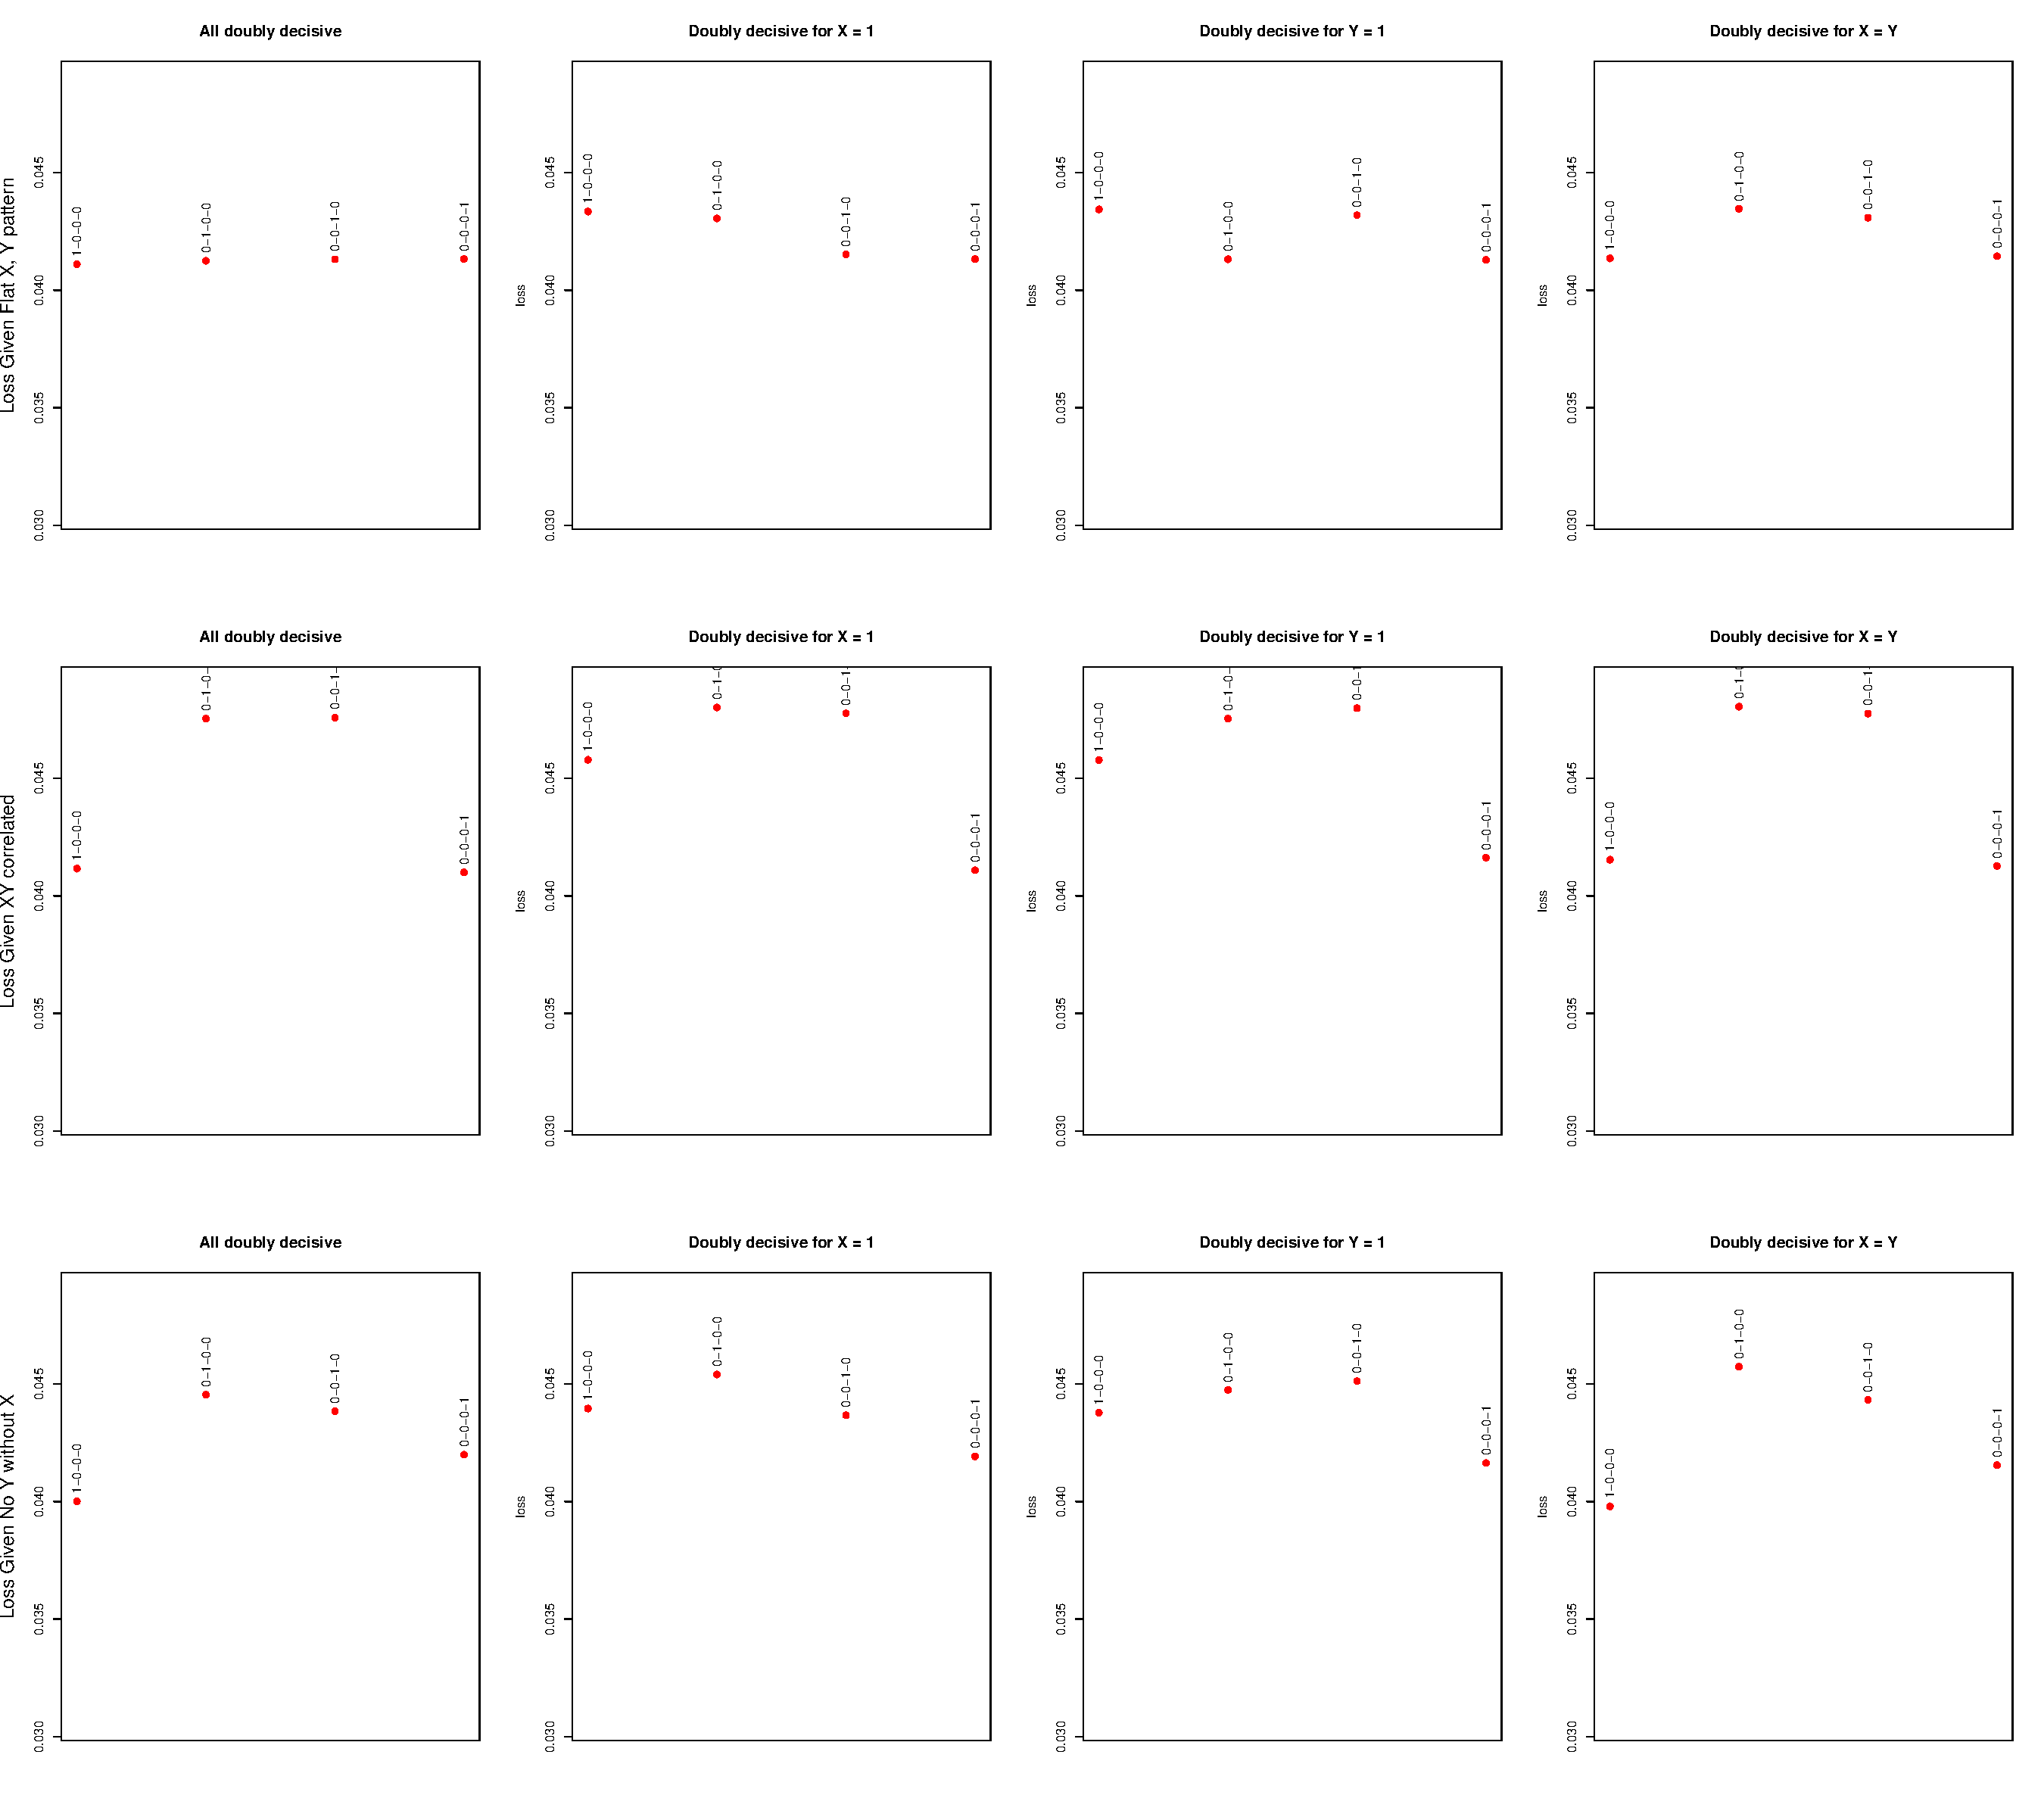
\includegraphics{Figures/K1.pdf}
\caption{Gains from different strategies involving process tracing in 1 case. We treat process tracing in a case as the search for one clue in that case, though this ``clue'' could be conceived of as a collection of clues that jointly have the probative value indicated. In each simulation, we start with 16 ``quantitative'' cases. Moving down the rows of graphs, we vary the distribution of these cases over an \(XY\) table. Moving across the columns of graphs, we vary the probative value of clue sought via process tracing.}
\end{figure}

More interesting patterns start emerging once we can choose two cases. We see the same two basic principles matter---go for probative value and for representativeness---but we now also see that there are complementarities in learning between different types of cases. In fact, for symmetric problems---as in the upper left panel, where the cases are evenly spread out and probative value is strong everywhere---we see a ranking between four families: first cases that fix \(Y\) (at 0 or 1) and spread on \(X\), second cases that fix \(X\) and spread on \(Y\), third cases that are on or off the diagonal, and fourth cases that focus on a single cell. Seeking clues on the diagonal does emerge as a good strategy (see for example the left figure in the middle row), but this appears to arise because the diagonal is data dense, not because there are particular complementarities of probative value there. In the bottom left figure for example, we see that in the case where there is data for \(X=1, Y=0\) but little data for \(X=0, Y=1\) , selecting cases distributed over the \(Y=0\) cells is about as informative as selecting on the diagonal. Selecting off the diagonal is one of the worst strategies here and is dominated by selecting all data from a dense cell.

Skip now to our graph of results where 4 cases are selected. As in previous figures we see strong gains for strategies that select cases proportionate to the size off cells. This is mot clear in the top left figure where one case per (equally sized) cell is the best strategy. More subtly it can be seen in the bottom left where the 2-0-1-1 strategy dominates --- this is a strategy that spreads roughly proportionately even if that means leaving some cells unrepresented. Strikingly in the base case various hybrid strategies do quite well, likely reflecting the fact that are as close to optimal spreads as possible. On and off diagonal strategies do poorly unless there is a strong diagonal, in which case these can dominate spreading across cells.

Overall relatively simple patterns emerge though these differ in some ways from text book suggestions. First focusing on probative value is key. Second seeking larger cells and balancing cases across cells appears fruitful. Third, and less intuitively, some combinations appear to gain more leverage than others. On and off diagonal strategies for example seem weaker in general than strategies that fix \(X\) or that fix \(Y\). Strategies that fix \(Y\) and allow variation on \(X\) seem strong, again, ceteris paribus.

Perhaps the most striking result from the simulations is that the optimal choice depends on many features. A simple rule, or even these core principles, may not get identify the right strategy. Ye the right strategy can be calculated, at least if one is willing to lay out beliefs on causal structure and probative value.

\begin{figure}
\centering
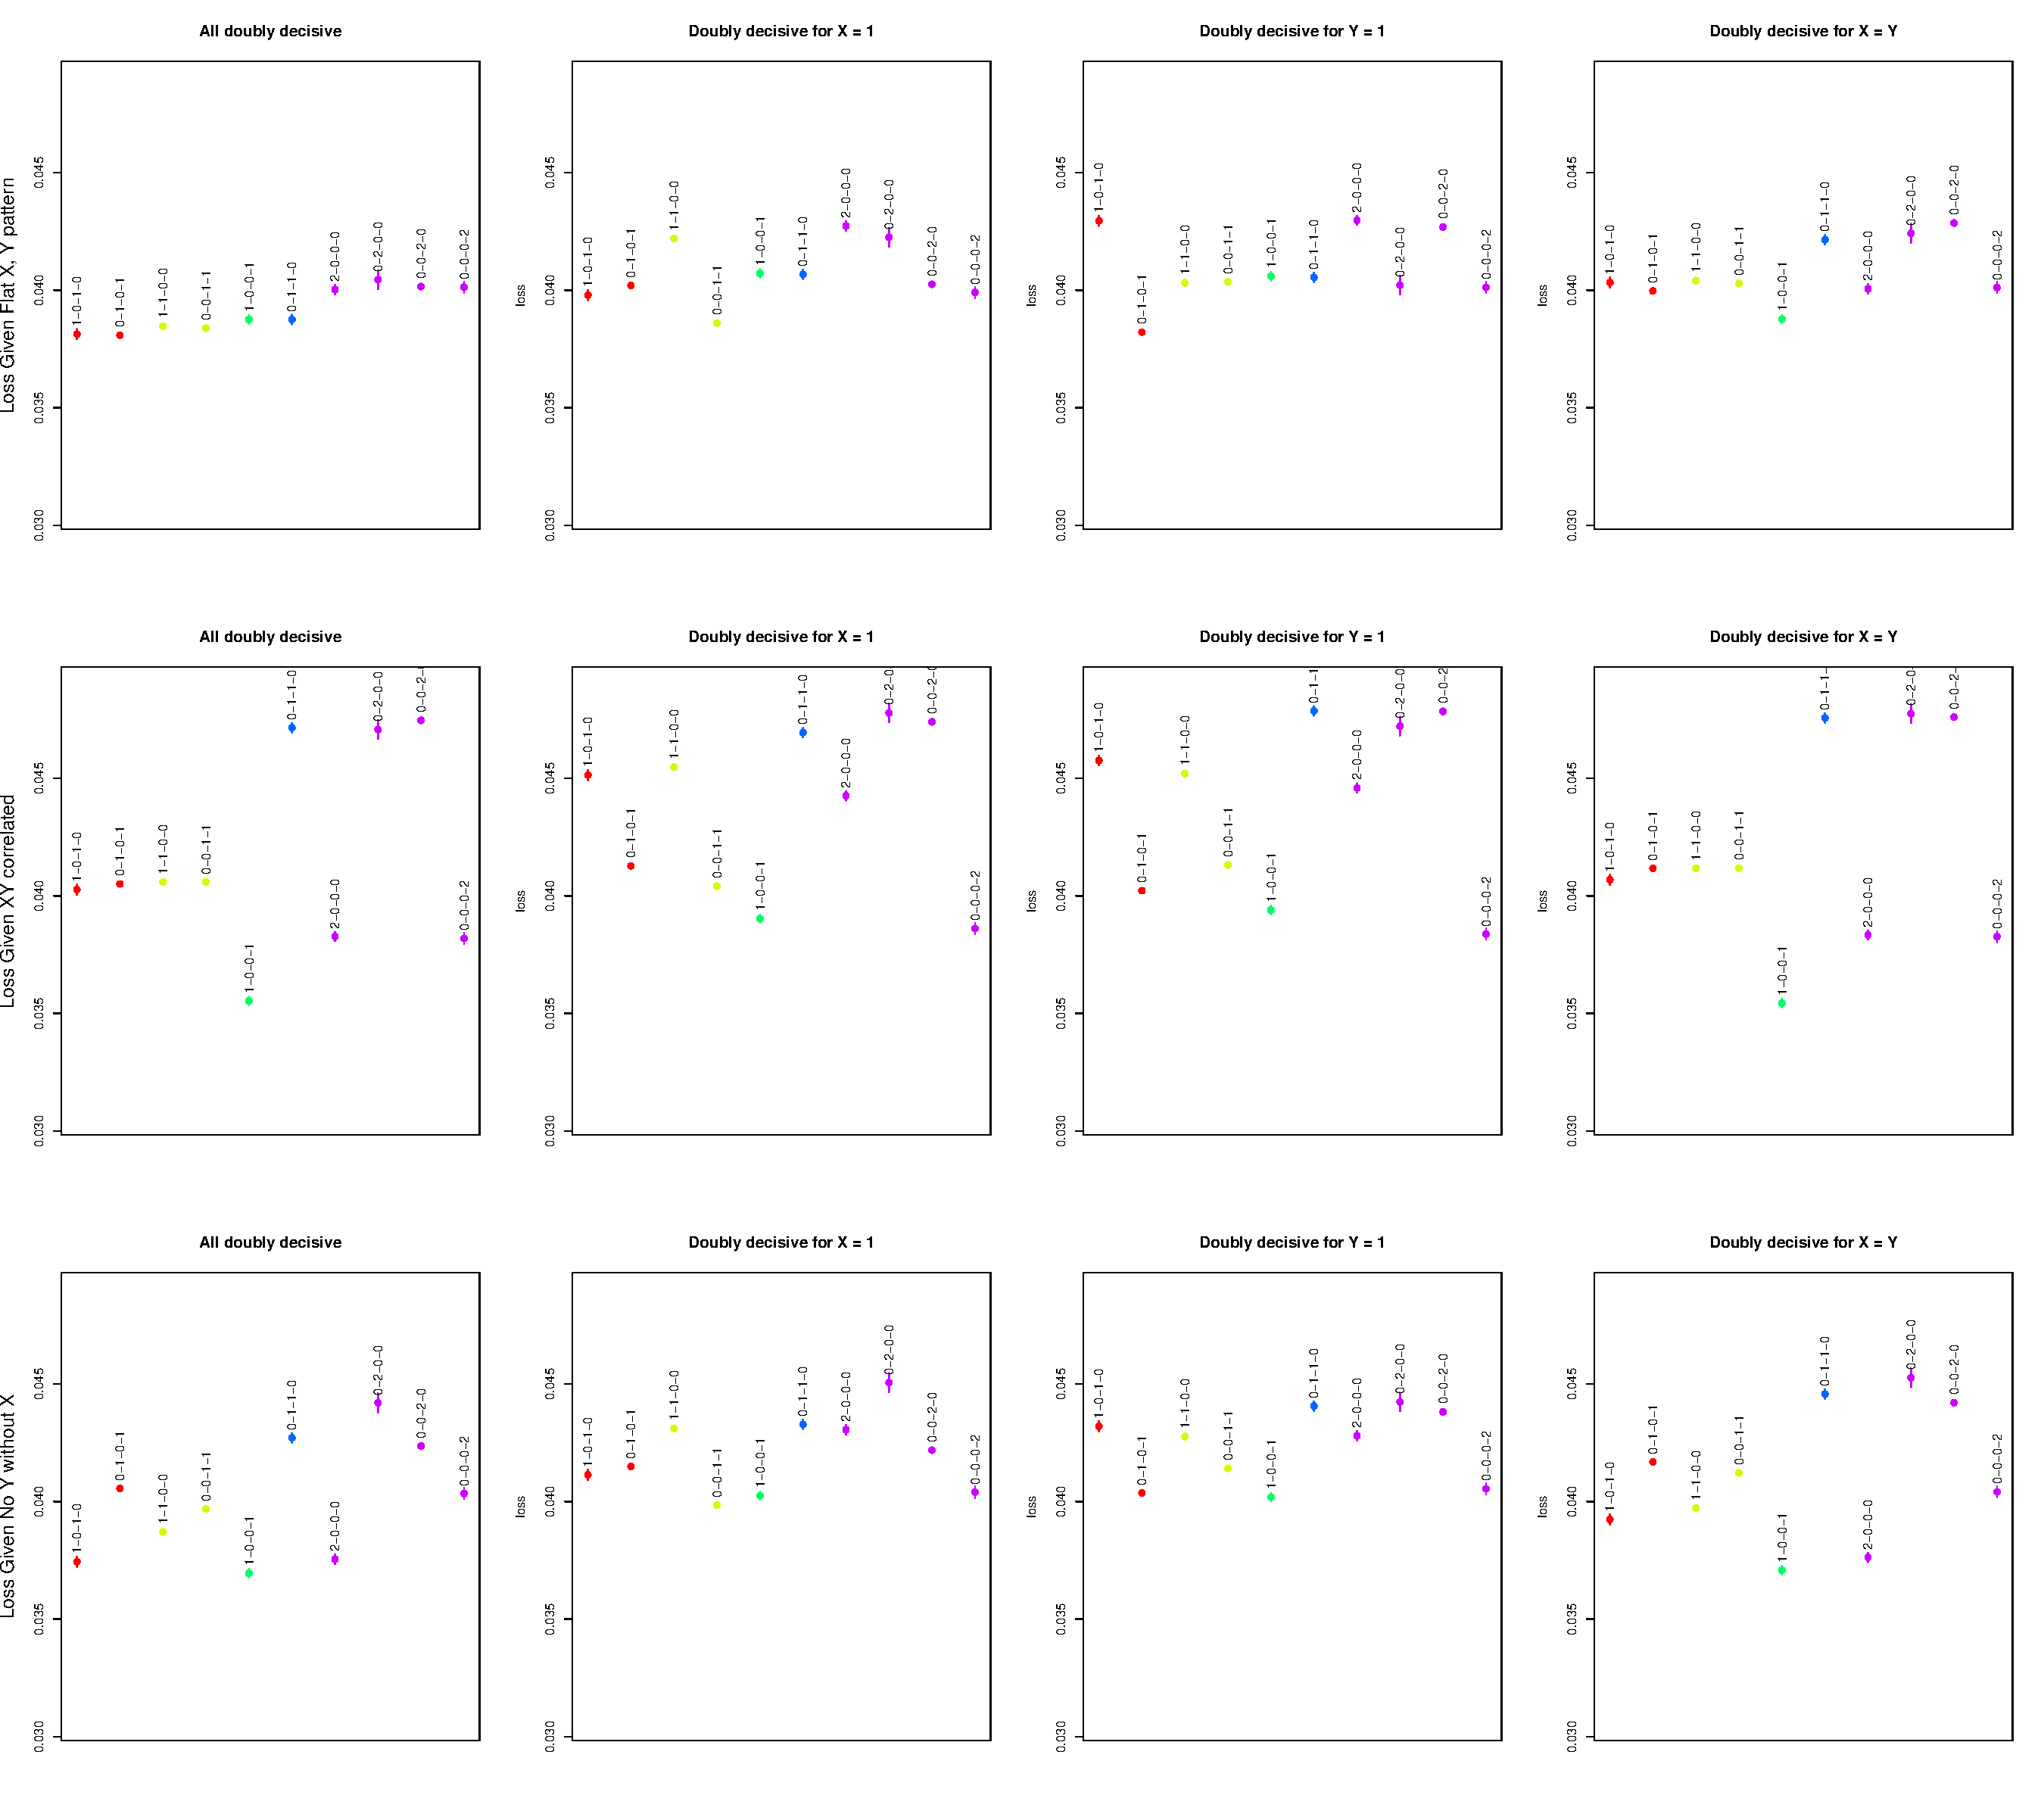
\includegraphics{Figures/K2.pdf}
\caption{Gains from different strategies involving process tracing in 2 cases. We treat process tracing in a case as the search for one clue in that case, though this ``clue'' could be conceived of as a collection of clues that jointly have the probative value indicated. In each simulation, we start with 16 ``quantitative'' cases. Moving down the rows of graphs, we vary the distribution of these cases over an \(XY\) table. Moving across the columns of graphs, we vary the probative value of clue sought via process tracing. Families of strategies are grouped and color-coded as follows: red=maximally dispersing across cells; yellow=}
\end{figure}

\begin{figure}
\centering
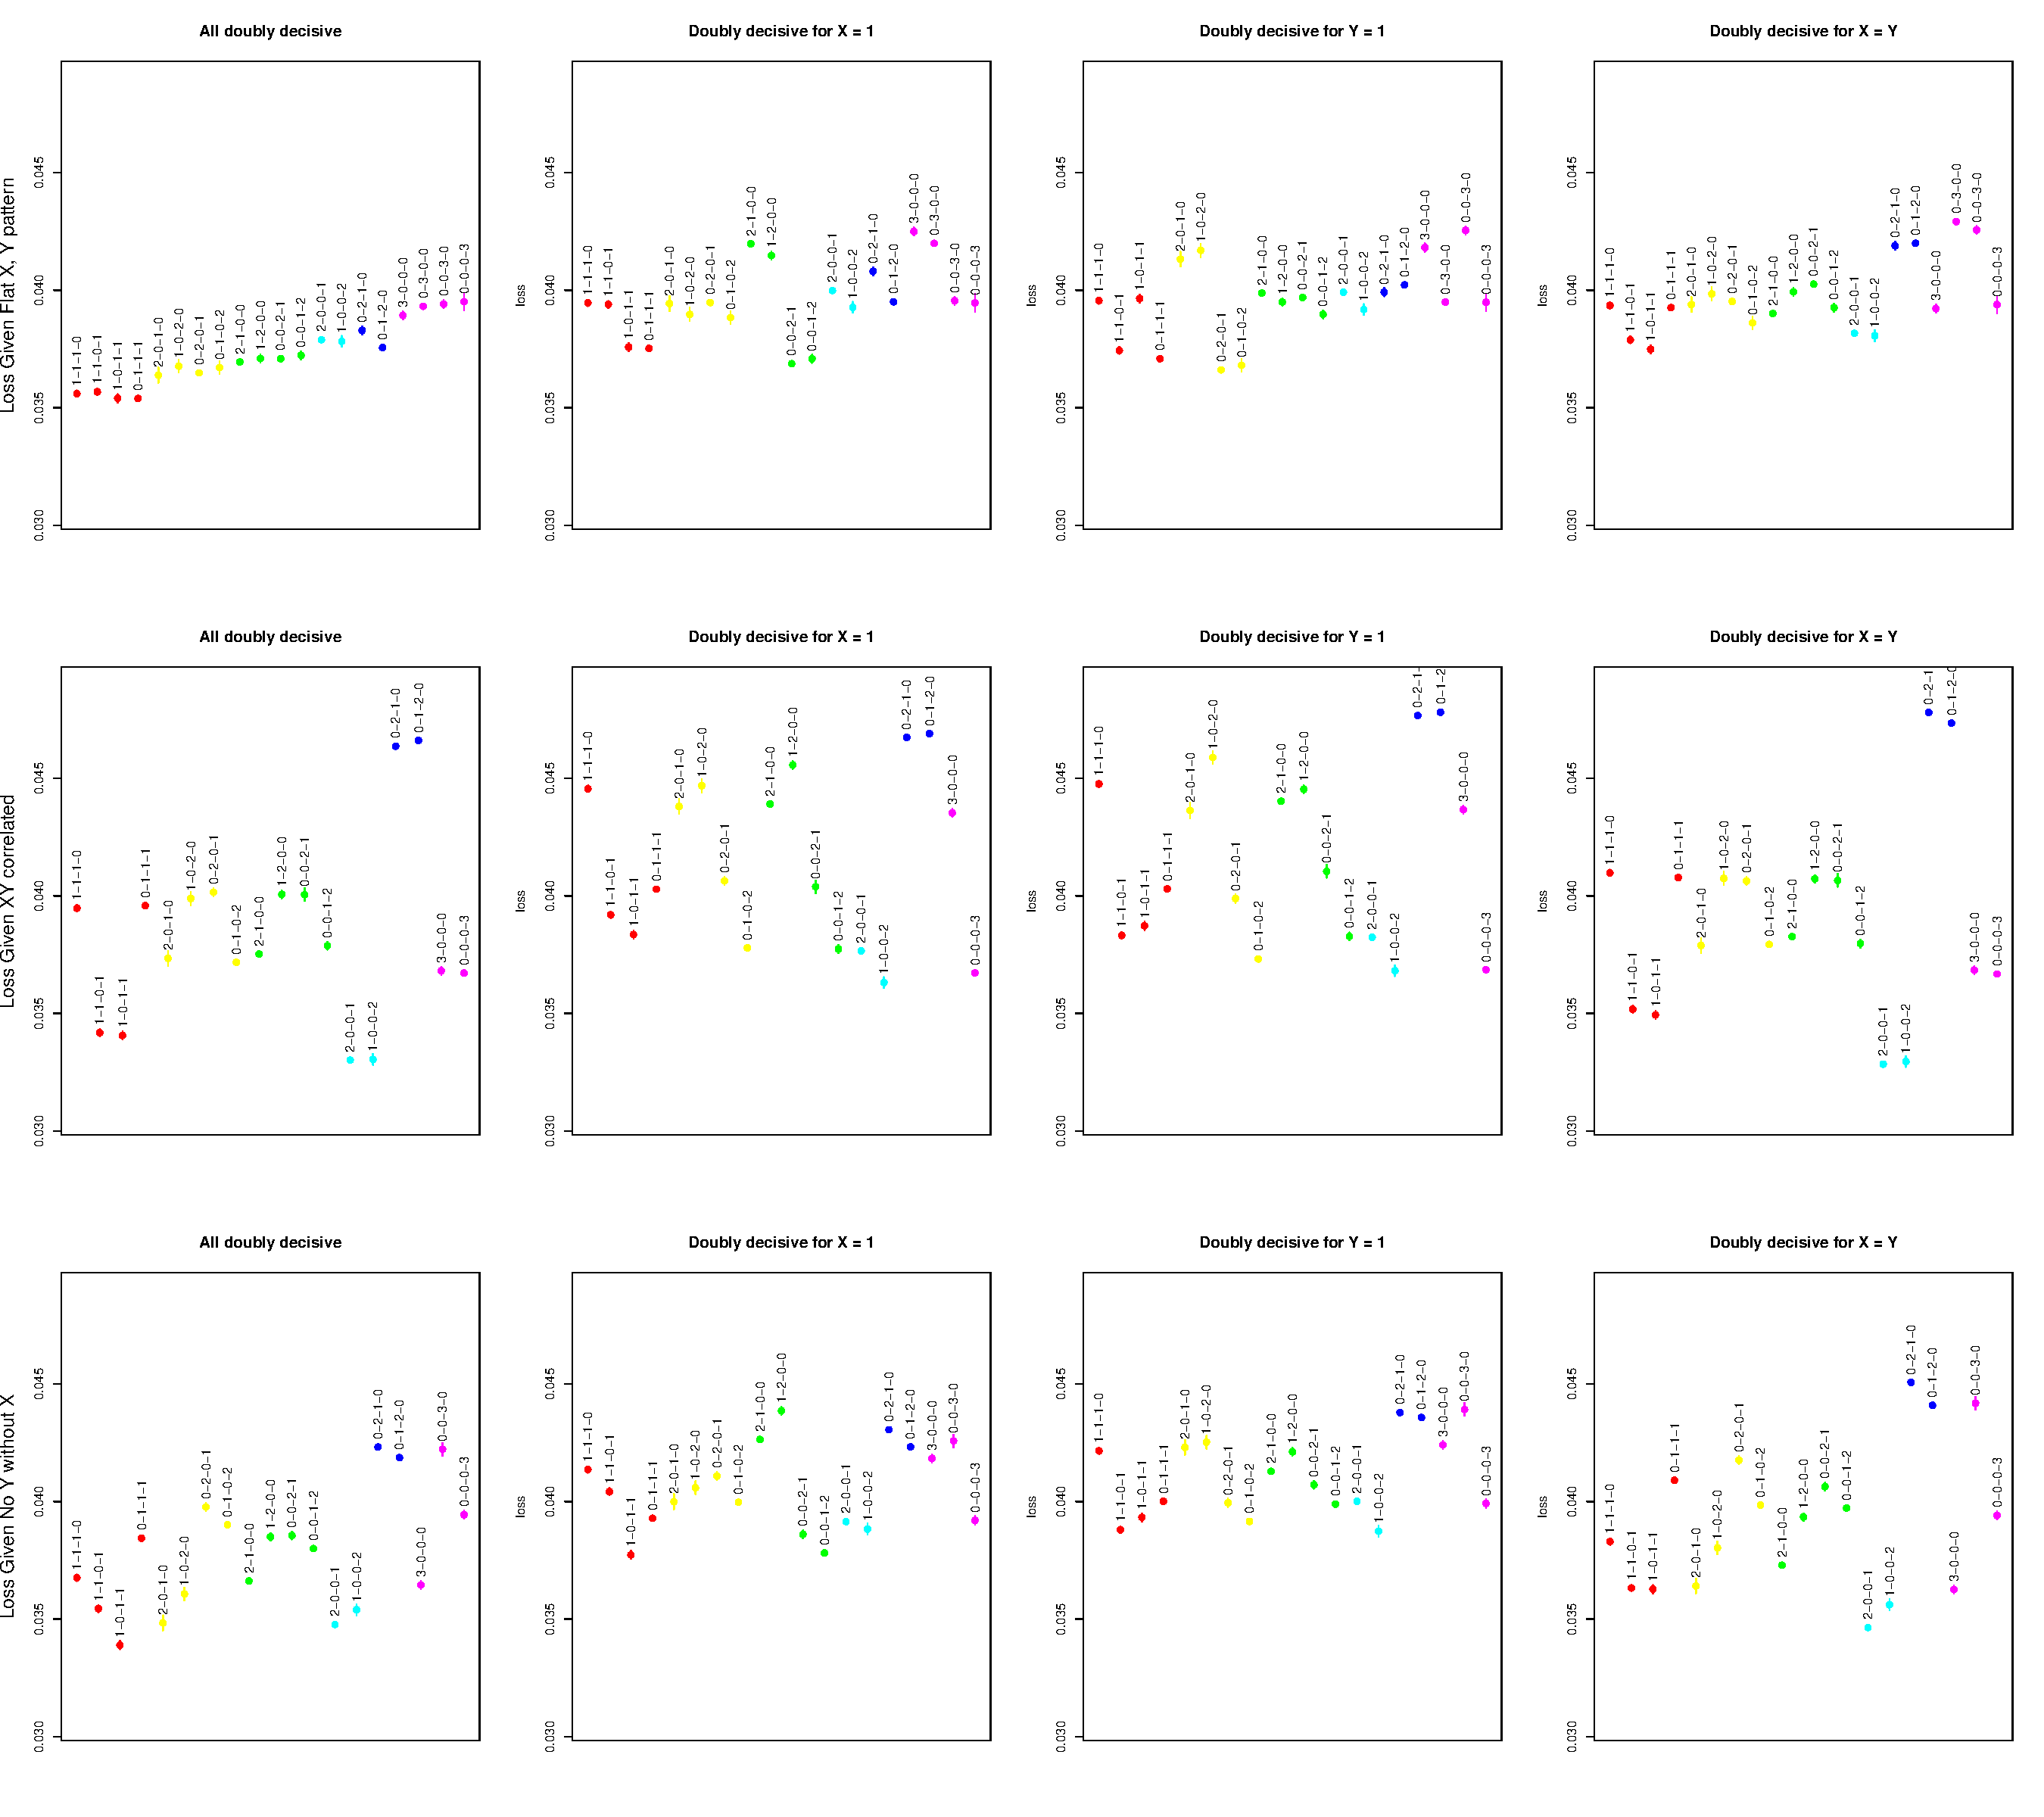
\includegraphics{Figures/K3.pdf}
\caption{Gains from different strategies involving process tracing in 3 cases. We treat process tracing in a case as the search for one clue in that case, though this ``clue'' could be conceived of as a collection of clues that jointly have the probative value indicated. In each simulation, we start with 16 ``quantitative'' cases. Moving down the rows of graphs, we vary the distribution of these cases over an \(XY\) table. Moving across the columns of graphs, we vary the probative value of clue sought via process tracing.}
\end{figure}

\begin{figure}
\centering
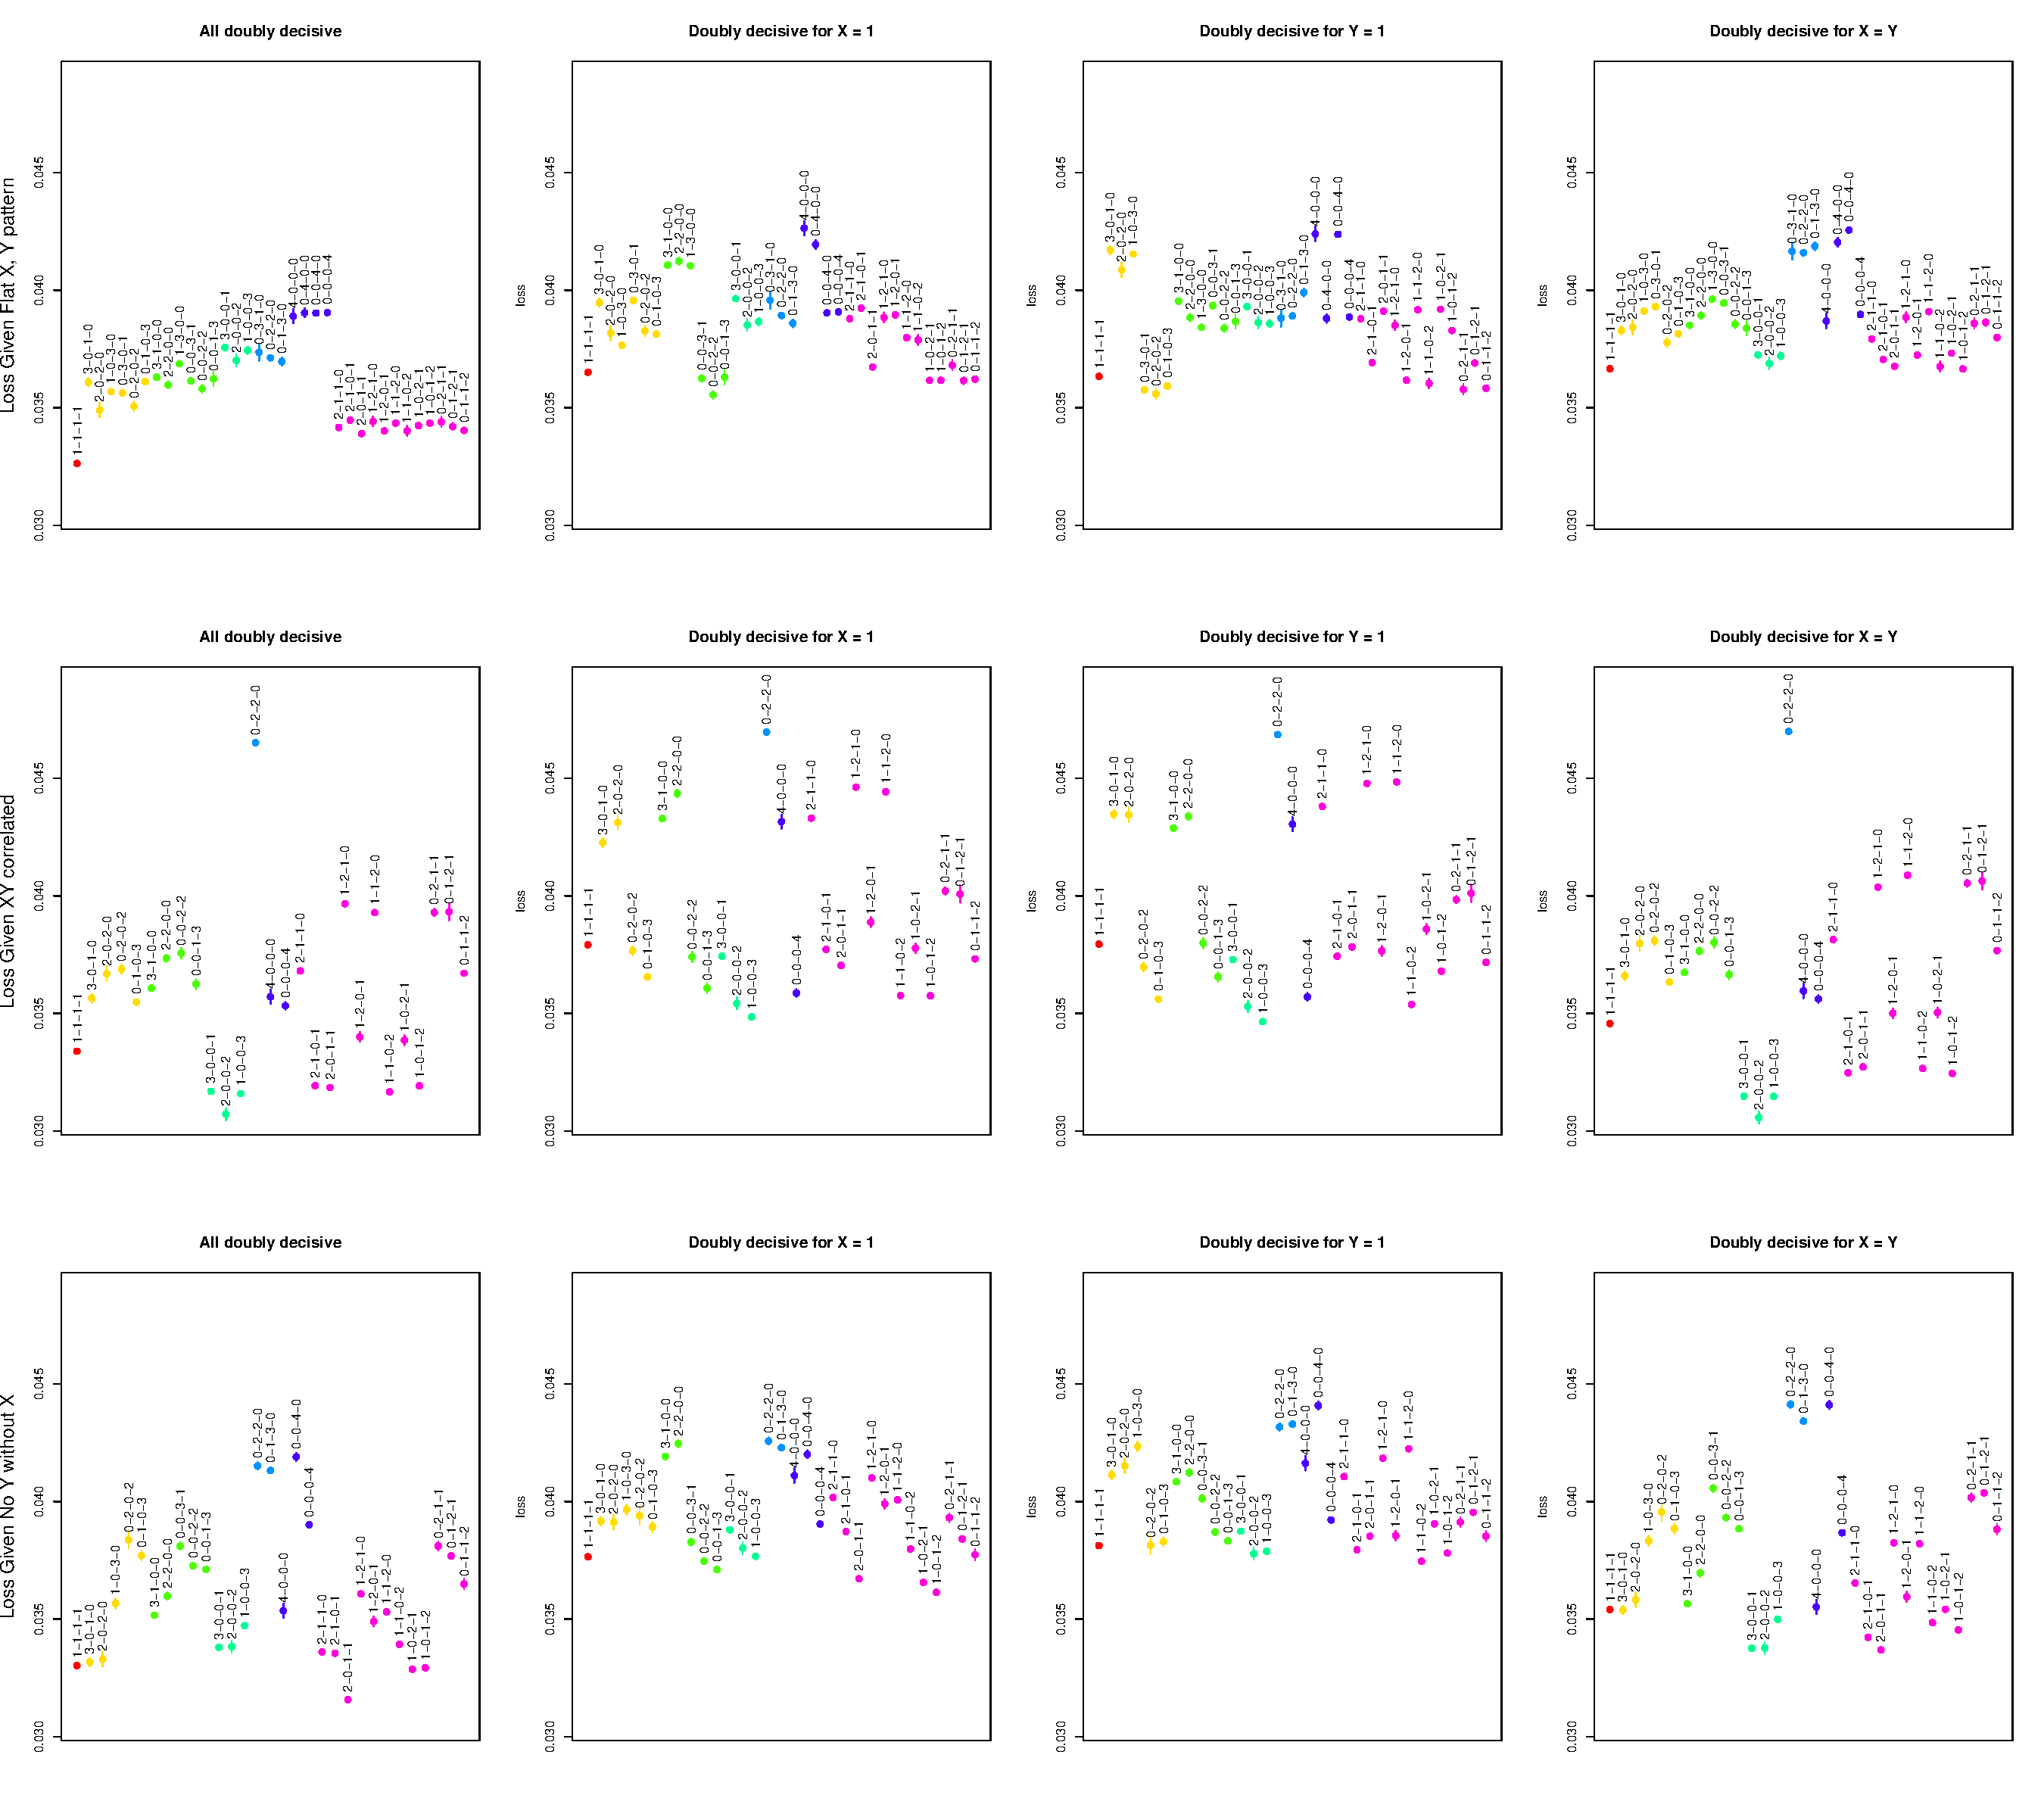
\includegraphics{Figures/K4.pdf}
\caption{Gains from different strategies involving process tracing in 4 cases. We treat process tracing in a case as the search for one clue in that case, though this ``clue'' could be conceived of as a collection of clues that jointly have the probative value indicated. Simulations invole 16 units distributed over an \(XY\) table in three patterns (rows) and variation over the probative value of different clues (columns).}
\end{figure}

\hypertarget{chapter-appendix-accounting-for-case-selection}{%
\section{Chapter Appendix: Accounting for case selection}\label{chapter-appendix-accounting-for-case-selection}}

\hypertarget{independent-case-selection-strategy}{%
\subsection{Independent case selection strategy}\label{independent-case-selection-strategy}}

We have focused on cases in which the researcher examines a fixed number of cases for clue information. An alternative strategy that produces a simpler likelihood is one in which each case is selected for within-case data gathering with some independent probability. The likelihood below introduces a case selection probability \(\kappa_{xy}\) that covers this case and allows for the possibility that selection probabilities are different for different \(X,Y\) combinations.

Thus we assume that \(X\), \(Y\) data is observed for all cases under study, but that \(K\) data may be sought for only a subset of these (we use the wildcard symbol '`\(*\)'' to denote that the value of the clue is unknown). We let \(n_{xyk}\) denote the number of cases of each type. Then, again assuming data is independently and identically distributed, the likelihood is:

\[\Pr(\mathcal{D}|\theta)= {\text{Multinomial}}(n_{000}, n_{001},n_{00*},n_{010}, n_{010},n_{01*}, n_{100}, n_{101},n_{10*},n_{110},n_{111} ,n_{11*} |
w_{000}, w_{001},w_{00*},w_{010}, w_{010},w_{01*}, w_{100}, w_{101},w_{10*},w_{110},w_{111} ,w_{11*})\]

where the event probabilities are now given by:

\[{\left( \begin{array}{c}
w_{000} \\ w_{001} \\  \vdots \\ w_{11*} \end{array} \right)=
\left( \begin{array}{c}
\lambda_b(1-\pi_b)\kappa_{00}(1-\phi_{b0}) + \lambda_c(1-\pi_c)\kappa_{00}(1-\phi_{c0})\\
\lambda_b(1-\pi_b)\kappa_{00}\phi_{b0} + \lambda_c(1-\pi_c)\kappa_{00}\phi_{c0}\\
\vdots \\
\lambda_b\pi_{b}(1-\kappa_{11}) + \lambda_d\pi_{d}(1-\kappa_{11})
\end{array} \right)}\]

Note we use a Greek symbol for the case selection probabilities to highlight that these may also be unknown and be an object of inquiry, entering into the vector of parameters, \(\theta\).

\subsubsection{Non-random $XY$ Sample Selection}\label{nonrandomcase}

While we have assumed in the canonical model that \(X,Y\) cases are selected at random, this need not be the case. Say instead that each case of type \(j\) is selected into the study with probability \(\rho_j\). In that case, assuming independent selection of cases for qualitative analysis, the likelihood function is now:

\[\Pr(\mathcal{D}|\theta) = {\text{Multinomial}}(n, w)\]
where: \[n = (n_{000}, n_{001},n_{00*},n_{010}, n_{010},n_{01*}, n_{100}, n_{101},n_{10*},n_{110},n_{111} ,n_{11*})\]

and the event probabilities, \(w\), are now, given by:

\[\left( \begin{array}{c}
w_{000} \\ w_{001} \\  \vdots \\ w_{11*}
\end{array} \right)=
\left( \begin{array}{c}
\frac{\rho_b \lambda_b}{\rho_a \lambda_a+\rho_b \lambda_b+\rho_c \lambda_c+\rho_d \lambda_d}(1-\pi_b)\kappa_{00}(1-\phi_{b0}) +
\frac{\rho_c \lambda_c}{\rho_a \lambda_a+\rho_b \lambda_b+\rho_c \lambda_c+\rho_d \lambda_d}(1-\pi_c)\kappa_{00}(1-\phi_{c0})\\
\frac{\rho_b \lambda_b}{\rho_a \lambda_a+\rho_b \lambda_b+\rho_c \lambda_c+\rho_d \lambda_d}(1-\pi_b)\kappa_{00}\phi_{b0}+
\frac{\rho_c \lambda_c}{\rho_a \lambda_a+\rho_b \lambda_b+\rho_c \lambda_c+\rho_d \lambda_d}(1-\pi_c)\kappa_{00}\phi_{c0}\\
\vdots \\
\frac{\rho_b \lambda_b}{\rho_a \lambda_a+\rho_b \lambda_b+\rho_c \lambda_c+\rho_d \lambda_d}\pi_{b}(1-\kappa_{11})+
\frac{\rho_d \lambda_d}{\rho_a \lambda_a+\rho_b \lambda_b+\rho_c \lambda_c+\rho_d \lambda_{11}}\pi_{d}(1-\kappa_{11})
\end{array} \right)\]

Note we have used a Greek symbol for the selection probabilities to highlight that these probabilities may be unknown and could enter into the set of parameters of interest, \(\theta\).

\hypertarget{conditional-random-case-selection}{%
\subsection{Conditional random case selection}\label{conditional-random-case-selection}}

Finally consider the likelihood for a design in which a researcher selects to search for clues as a function of the \(X,Y\) data. This is a somewhat harder case because the size of each \(X,Y\) group is stochastic. Let \(n_{xy} = n_{xy0}+n_{xy1}+n_{xy*}\) denote the number of cases with particular values on \(X\) and \(Y\), and let \(n_{XY}=(n_{00},n_{01},n_{10},n_{11})\) denote the collection of \(n_{xy}\) values.

Say now that conditional on the \(X,Y\) observations, a researcher sets a target of \(k_{xy}(n_{XY})\) cases for clue examination (note here that the number of clues sought for a particular \(X,Y\) combination can be allowed to depend on what is observed across all \(X\), \(Y\) combinations). Then the likelihood is:
\[\text{Multinomial}(n_{XY}|w_{XY})\prod_{x\in\{0,1\},y \in\{0,1\}}\text{Binom}(n_{xy1}|k_{xy}(n_{xy}), \psi_{xy1})\]

The multinomial part of this expression gives the probability of observing the particular \(X,Y\) combinations; the event probabilities for these depend on \(\lambda\) and \(\pi\) only \textbar{} for example \(w_{11} = \lambda_b \pi_b+\lambda_d \pi_d\). The subsequent binomials give the probability of observing the clue patterns conditional on searching for a given number of clues (\(k_{xy}(n_{xy})\)) and given an event probability \(\psi_{xy1}\) for seeing a clue given that the clue is sought for an \(x,y\) combination; thus for example:
\[ \psi_{111} = \frac{\lambda_b \pi_b}{\lambda_b \pi_b+\lambda_d \pi_d} \phi_{b1} + \frac{\lambda_d \pi_d}{\lambda_b \pi_b+\lambda_d \pi_d} \phi_{d1}\]

\hypertarget{part-models-in-question}{%
\part{Models in Question}\label{part-models-in-question}}

\hypertarget{where-does-probative-value-come-from}{%
\chapter{Where does probative value come from?}\label{where-does-probative-value-come-from}}

\begin{center}\rule{0.5\linewidth}{\linethickness}\end{center}

We outline strategies to reduce reliance on unfounded beliefs about the probative value of clues.

\begin{center}\rule{0.5\linewidth}{\linethickness}\end{center}

Everything we have talked about so far assume that researchers are able to state priors on all the primitives entering into the analysis.

But what if they cannot?

As we have noted, learning in the framework we have described can occur even with ``flat'' priors over causal effects and assignment probabilities. However priors on the probative value of clues have to be informative. We also suspect, however, that researchers usually have---or could readily formulate---a rough idea of where they believe the parameter values lie. They have approximate prior beliefs about whether a causal effect is very common or not very common; whether confounding is likely or unlikely; and whether a given feature of a process is highly likely to be observed, moderately likely to be observed or very unlikely to observed under a given causal theory. Indeed, beliefs about these last two parameters already play a central role in standard approaches to correlational analysis and process tracing. This means that researchers should be in a position to specify a limited range of plausible values for each of the model's primitives. They can then use the model to explore the consequences of different values in this plausible range either for their findings (given a set of collected data) or for their research design choices (prior to collecting data). And they can express their conclusions explicitly as \emph{conditional} on their priors, or report findings for a range of prior values. Even where researchers are reluctant to quantify their beliefs, we believe that the principles underlying the BIQQ approach can nonetheless offer valuable, heuristic guidance on how to interpret mixes of qualitative and quantitative evidence in ways that are internally consistent and make more complete use of the available information.

At the same time, it is consequential where researchers' priors---in particular, their priors on the probabilities of clues---come from: whether they reflect some form of empirical knowledge or derive purely from theory. If a theory \(T\) suggests that clue \(K\) will be observed if and only if \(X\) causes \(Y\), then the presence of \(K\) provides evidence that \(X\) causes \(Y\) \emph{only to the extent that \(T\) provides a true account of the causal logic through which \(X\) affects \(Y\)}. If \(T\) captures the wrong mechanism of causation, for instance, then clue probabilities that derive from the theory may be wrong and causal inferences that are based on the observation of these clues will be wrong. To use process data to make claims about causal effects that are \emph{not} conditional on theories, researchers need empirical support for claims on the probative value of clues. This may often be difficult to obtain. In particular, it requires that \{knowledge travel\}: whereas in traditional Bayesian analysis researchers often employ uninformative (flat) priors, the use of clue-based data contributes to analysis \emph{only if} priors are informative.

Finally, we believe that the model is useful in part \emph{because} it places such high demands on scholars' beliefs about the probative value of within case data: that is, because it clearly identifies the required inputs into the process of drawing integrated causal inferences. Put differently, to the extent that scholars are unable to specify even approximate ranges on these parameters, this is a problem for causal inference, not a problem for the model. The framework thus has implications for research agendas in identifying the kinds of knowledge that scholars need to generate if they are to use mixed methods to provide causal accounts of the world.

\hypertarget{causal-discovery}{%
\section{Causal discovery}\label{causal-discovery}}

\hypertarget{the-possibility-of-identification-of-probative-value-from-experimental-data}{%
\section{The possibility of identification of probative value from experimental data}\label{the-possibility-of-identification-of-probative-value-from-experimental-data}}

Imagine we had access to infinite experimental data on the effect of \(X\) on \(Y\) and we want to know for a case (exchangeable with any other in this population) with \(X=Y=1\), whether \(X=1\) caused \(Y=1\)--- PC. Our experimental data can be written as a transition matrix as follows:

\[P^{u}=\left( \begin{array}{cc} 0.50 & 0.50 \\ 0.25 & 0.75 \end{array}\right)\]
If we have prior beliefs about the distribution of causal types, then PC would be simply \(\frac{\lambda^u_b}{\lambda^u_b + \lambda^u_d}\).

But let's assume we cannot justify such beliefs. In this case, from results in MURTAS REF, we can still place bounds on PC:

\[\frac13 \leq PC \leq \frac23 \]
For intuition note that \(P^{xy}\) implies a causal effect of .25 and so the lowest value of \(\lambda_b^u\) consistent with \(P^{xy}\) arises when \(\lambda_b^u = .25\) and \(\lambda_a^u = 0\), in which case \(\lambda_c^u = .25\) and \(\lambda_d^u = .5\). In this case \(\lambda_b^u/(\lambda_b^u+ \lambda_d^u)=\frac{1}{3}\). The highest consistent value of \(\lambda_b^u\) arises when \(\lambda_b^u = .5\) and \(\lambda_a^u = .25\), in which case \(\lambda_c^u = 0\) and \(\lambda_d^u = .25\). In this case \(\lambda_b^u/(\lambda_b^u+ \lambda_d^u)=\frac{2}{3}\).

Say now we have access to auxiliary data \(K\) and plan to make inferences based on \(K\).

We will suppose first that \(K\) is a moderator and second that \(K\) is a mediator.

\hypertarget{moderator}{%
\subsection{Moderator}\label{moderator}}

Consider first a situation in which our case is drawn from a set of cases for which \(X\) adn \(K\) were each randomly assigned. Say then that the transition matrices, conditionl on \(K\) look as follows:

\[P^{K=0}=\left( \begin{array}{cc} 0 & 1 \\ 0.5 & 0.5 \end{array}\right), P^{K=1}=\left( \begin{array}{cc} 1 & 0 \\ 0 & 1 \end{array}\right)\]
In this case we can now identify PC, even before observing \(K\). If \(K=0\), PC is 0---there are no cases with positive effects in this condition. If \(K=1\) PC = 1. We have a prior that \(K=1\) of .5 and after observing \(X=Y=1\) we raise this to \(2/3\). Thus our prior belief on \(PC\) --- before seeing \(K\)--- is \(2/3 * 1 + 1/3 * 0 = 2/3\).

How about \(\phi_{b1}\) and \(\phi_{d1}\)?

Here positive effects only arise when \(K=1\) and so \(\phi_{b1} = 1\). \(Y=1\) without being cause by \(X\) only if \(K=0\) and so \(\phi_{b0} = 0\). Thus we have a double decisive clue.

\hypertarget{mediator}{%
\subsection{Mediator}\label{mediator}}

Consider now a case with mediation. Say now that \emph{in addition} we know from experimental data, that \(K\) mediates the relationship between \(X\) and \(Y\); indeed we will assume that we have a case of complete mediation, such that, conditional on \(K\), \(Y\) does not depend on \(X\). The transition matrices from \(X\) to \(K\) and \(K\) to \(Y\) are:

\[P^{xk}=\left( \begin{array}{cc} 1 & 0 \\ 1/2 & 1/2\end{array}\right), P^{ky}=\left( \begin{array}{cc} 1/2 & 1/2 \\ 0 & 1\end{array}\right)\]
Even without observing \(K\), this information is sufficient to place a prior on PC of \(p=\frac13\).

To see this, note that we can calculate:

\begin{itemize}
\tightlist
\item
  \(\lambda_a^K =0\), \(\lambda_b^K = \frac{1}{2}\), \(\lambda_c^K = \frac{1}{2}\), \(\lambda_d^K = 0\)
\item
  \(\lambda_a^Y =0\), \(\lambda_b^Y=\frac{1}{2}\), \(\lambda_c^Y=0\), \(\lambda_d^Y=\frac{1}{2}\)
\end{itemize}

and so:

\begin{itemize}
\tightlist
\item
  \(\lambda_b^u = \lambda_b^K\lambda_b^Y = \frac{1}4\)
\item
  \(\lambda_d^u = \lambda_d^Y\)
\item
  \(p = \frac{\lambda_b^u}{\lambda_b^u + \lambda_d^u} = \frac{1}3\).
\end{itemize}

whence:

\begin{itemize}
\tightlist
\item
  \(\phi_{b1} = 1\)
\item
  \(\phi_{d1} = \lambda_d^K + \lambda_b^K = \frac{1}{2}\)
\end{itemize}

\hypertarget{generally-not-so-easy}{%
\subsection{Generally not so easy}\label{generally-not-so-easy}}

Thus we can \emph{in principle} calculate the \(\phi\)s from experimental data given a mediation process. In this case we get a strong hoop test.

Note that this agrees with the calculation of \(PC|K\) in MURTAS REF, which does not make use of a calculation of \(\phi\)s.

\[PC | K = 1 = \frac{\phi_b p}{\phi_b p + \phi_d (1-p)} = \frac{1 \times\frac13}{1 \times\frac13 + \frac{1}{2} \times \frac23}  = \frac{1}{2}\]

\hypertarget{bounds-on-causes-of-effects}{%
\section{Bounds on causes of effects}\label{bounds-on-causes-of-effects}}

We are interested in quantities such as \(\phi_{b1}, \phi_{d1}\)---the probability that \(K=1\) given \(X\) caused \(Y\) and \(X=Y=1\) in a model with mediation. \protect\hyperlink{eq:phis_from_lambdas}{Equation} gave expressions for this when the \(\lambda\)s were known.

What if they are not?

In this case it can be possible to calculate the bounds on \(\phi_{b1}, \phi_{d1}\). Consider a chain with transition matrices \(P(\tau_1, \sigma_1), P(\tau_2, \sigma_2)\). We are interested in:

\[\phi_{b1} = \frac{\lambda_{b}^K\lambda_{b}^Y}{\lambda_{b}^K\lambda_{b}^Y + \lambda_{a}^K\lambda_{a}^Y}\]

Noting that \(\tau_j = \lambda_{b_j} - \lambda_{a_j}\), and \(\tau\) is known.

\[\phi_{b1} = \frac{\lambda_{b}^K\lambda_{b}^Y}{\lambda_{b}^K\lambda_{b}^Y + (\lambda_{b}^K-\tau_1)(\lambda_{b}^Y - \tau_2)}\]
which we can see is decreasing in \(\lambda_{b_j}\) (this may seem counterintuitive, but hte reason is that with \(\tau_j\) fixed, lower \(\lambda_{b_j}\) also means lower \(\lambda_{a_j}\) which means less ambiguity about \emph{how} \(X\) affects \(Y\) (ie through positive or negative effects on \(K\)).

The lowest permissible value of \(\lambda_{b_j}\) is \(\tau_j\), yielding \(\phi_1 = 1\).

The highest value obtainable by \(\lambda_{b_j}\) is when \(\lambda_{a_j} = \frac{1-\tau_j+\rho_j}2\) and so \(\lambda_{b_j} = \frac{1+\tau_j+\rho_j}2\).

In this case:
\[\phi_{b1} = \frac{(1+\tau_1+\rho_1)(1+\tau_2+\rho_2)}{(1+\tau_1+\rho_1)(1+\tau_2+\rho_2) + (1-\tau_1+\rho_1)(1-\tau_2+\rho_2)}= \frac{(1+\tau_1+\rho_1)(1+\tau_2+\rho_2)}{2(1+\rho_1)(1+\rho_2) + 2\tau_1\tau}\]

And so:

\[\frac{(1+\tau_1+\rho_1)(1+\tau_2+\rho_2)}{2(1+\rho_1)(1+\rho_2) + 2\tau_1\tau_2} \leq \phi_{b1} \leq 1\]
These are the bounds on \(\phi_{b1}\). We can calculate bounds on \(\phi_{d1}\) in a similar way---though of course these are not independent.

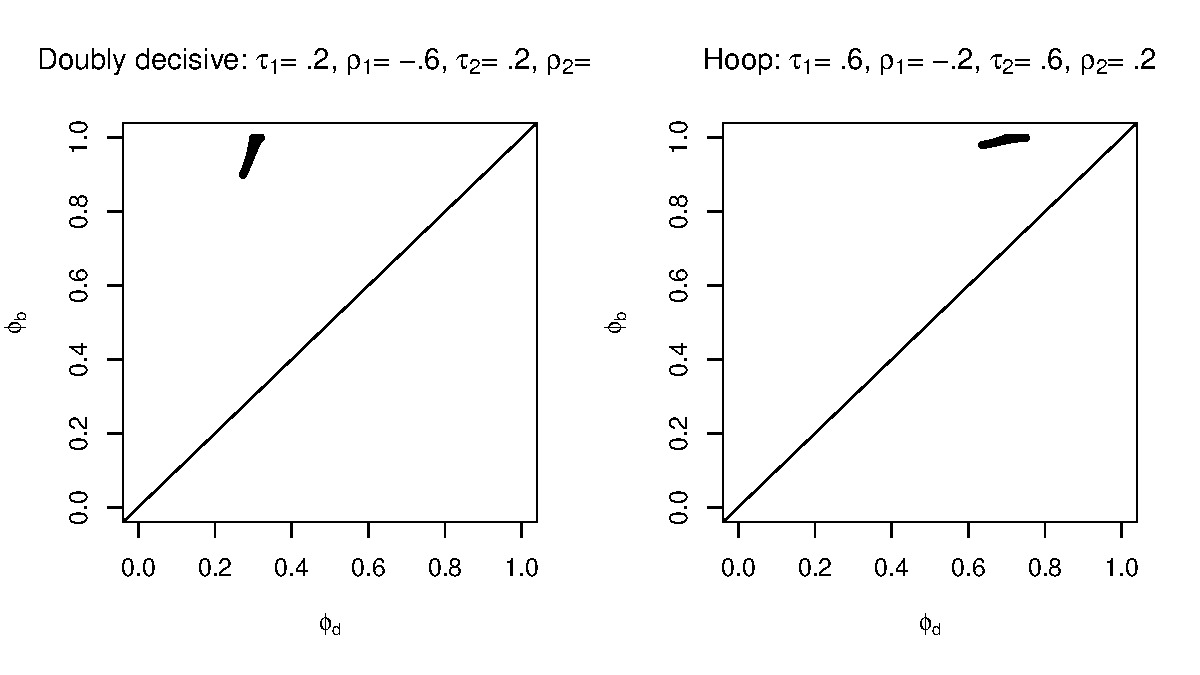
\includegraphics{ii_files/figure-latex/unnamed-chunk-88-1.pdf} 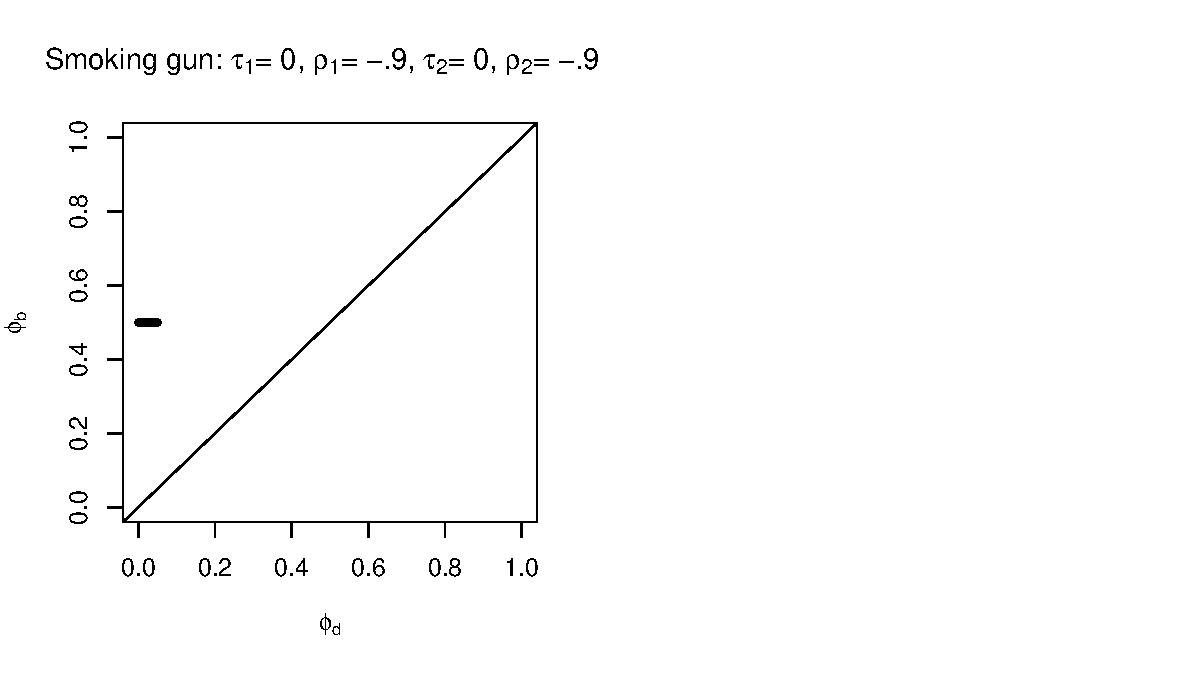
\includegraphics{ii_files/figure-latex/unnamed-chunk-88-2.pdf}

\[\phi_{d1} = \frac{\lambda_{b}^K\lambda_{d}^Y}{(\lambda_{a}^K + \lambda_{b}^K + \lambda_{c}^K)\lambda_{d}^Y+ \lambda_{c}^K\lambda_{a}^Y}\]

For the smoking gun, \(\phi_{b1}\) is .5 because \(\lambda_a^j = \lambda_b^j\) exactly; \(\phi_{d1}\) might be low as \(d\) types mostly arise because of \(c\) types in the first step and \(a\) types in the second.
.

this is achived with a low value of \(\lambda_{d}^Y\)

Whether the bounds map into useful probabitve value depends in part on whether causal effects are better identified in the first or the second stage.

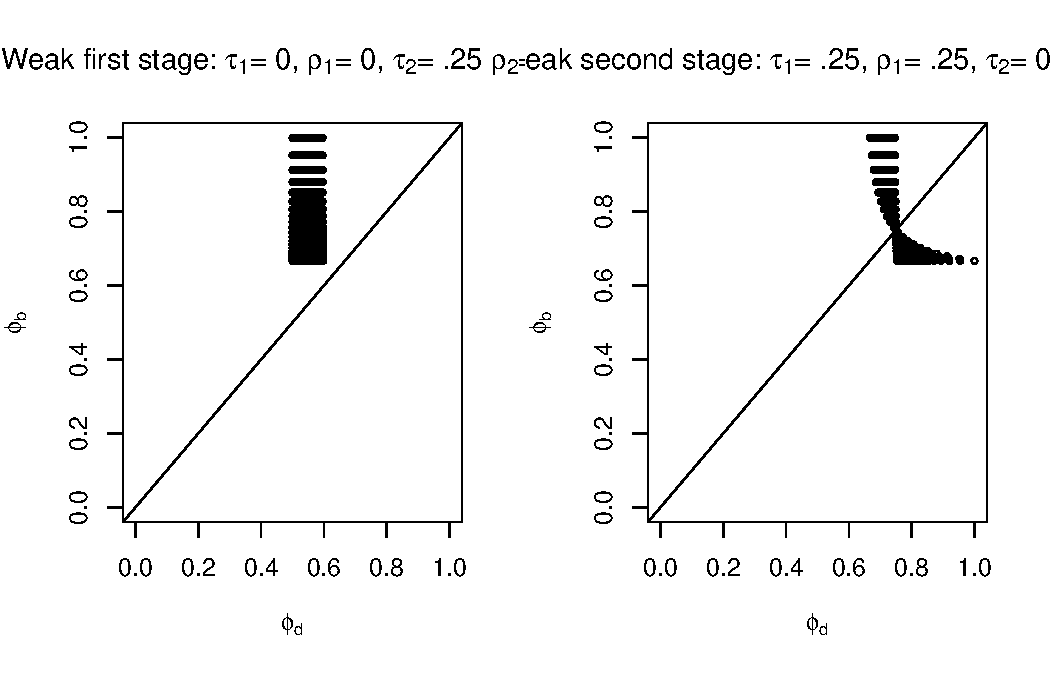
\includegraphics{ii_files/figure-latex/unnamed-chunk-90-1.pdf}

\hypertarget{qualitative-beliefs-and-sensitivity-analyses}{%
\section{Qualitative beliefs and Sensitivity Analyses}\label{qualitative-beliefs-and-sensitivity-analyses}}

A first strategy to address concerns around weak foundations for claims on probative value---even after attempting to introduce information on uncertainty around probative value, is to assess the extent to which conclusions depend on the details of information provided. In some cases conclusions may be very sensitive to details provided; in other cases not so much.

For a simple illustration, say one's prior is that it is equally likely that a case is a \(B\) or \(D\) type. Say one thinks that \(\phi_D=0\) and so seeing a clue provides a smoking gun test. Then conditional on seeing the clue, the conclusion is the same no matter what the actual value of \(\phi_B\)---as long as \(\phi_B>0\). The details do not matter in this (albeit extreme case). In this case if a clue is not see then the conclusions can depend quite strongly on the value of \(\phi_B\) however: the posterior could range from \(0.5\) in the case where \(\phi_B=0\) (and so the clue is not informative at all) to \(0\) in the case where \(\phi_B = 1\) (and so the clue is double decisive). Thus how sensitive conclusions are to beliefs depend very much on the data at hand.

For a larger \(n\) illustration, refer back to our example of large \(n\) data in chapter 9 where we saw that when there is confidence around assignment probabilities (as for example in an RCT) then, with large \(N\), conclusions do not depend strongly on clue information about a handful of cases, no matter what the probative value.

More generally there is a literature on probabilistic causal models that assess the scope for inferences when researchers provide ranges of plausible values for parameters (perhaps intervals, perhaps only signs, positive negative, zero), rather than specifying a probability distribution. For a comprehensive treatment of qualitative algebras, see \citet{parsons2001qualitative}. Applied to the example above we might imagine a researcher willing to say that they think \(\phi_B\) is not plausibly greater than .5, but unwilling to make a statement about their beliefs about where in the \(0\) to \(0.5\) range it lies. In this case, with the other parameter values outlined above the conclusions will lie in \(0.5\) and \(0.33\)---ruling out half the possible ranges on the parameter results in a ruling out of a two thirds of the possible range of the conclusion.

\hypertarget{conditional-claims}{%
\section{Conditional claims}\label{conditional-claims}}

A second response is to clearly communicate the contingent nature of claims. As we outlined in Chapter 4, some causal models might reasonably reflect actual beliefs about the world---for example one might, be convinced that a treatment was randomly assigned, that there is no interference, and that units are independently sampled from a distribution of types. All of these beliefs may be unwise. But if help, then the simple DAG in chapter 4 (REF) can be taken to represents beliefs about the world rather than a model of the world, in the sense of a simplified representation. But as we noted in Chapter 4, for an even modestly more complex situation, it seems inevitable that the model being used is truly a model and not a faithful summary of beliefs.

Owning the model in this way results in a useful reposing of the question: the question becomes not whether the assumptions are correct but whether the model is useful \citep{clarke2012model}. That is the subject of Chapter 13.

\hypertarget{learning-about-parameters-within-a-model}{%
\section{Learning about parameters within a model}\label{learning-about-parameters-within-a-model}}

The general approach outlined in the literature on probabilistic graph allows for considerable flexibility on what is fixed and what is not. As we described in Chapter 2, any seemingly fixed feature of a structural equation can become a quantity of interest in a lower level model. In our baseline model\footnote{Some individuals are observed to have received a treatment (\(X\)) while others have not. Assume that, subsequently, a researcher observes outcomes (\(Y\)) for all units. Assume that each unit belongs to one of four unobserved `'types,'' \(A\) (adverse), \(B\) (beneficial), \(C\) (chronic), \(D\) (destined) with potential outcomes \(Y(0)=1, Y(1)=0\) for type \(A\); \(Y(0)=0, Y(1)=1\) for type \(B\); \(Y(0)=0, Y(1)=0\) for type \(C\); and \(Y(0)=1, Y(1)=1\) for type \(D\). As in the canonical model, researchers have access to data on a third variable, \(K\) and we let \(\phi_{tx}\) denote the probability of observing \(K\) for type \(t\) given \(X=x\).} for instance the probative value of clues, as captured by terms \(\phi_{tx}\), are parameters over which researchers update; they do not uniquely derive from external information.

How much external information has to be brought in to learn from clues? Does any external information need to be brought in? We address the question by considering situations where researcher have \emph{uninformative} priors about treatment effects \emph{and} over the probative value of clues. We simplify the problem by assuming that assignment probabilities are known (specifically we set these at 0.5 for all units) and we assume that there is infinite data available for analysis. Note that under these conditions the average treatment effect (\(b-a\)) can be estimated with certainty using information about \(X\) and \(Y\) only.

We are interested in whether data on clues, \(K\) can be used to make estimates of the size of the causal types, \(a,b,c,d\) and whether the data allows us to estimate the probative value of clues. Let \(\theta\) denote our parameter vector containing causal types, \((\lambda)\) and probative values \(\phi_{tx}\).

We find that when priors over clue probabilities do not discriminate between causal types, then learning clue values does not affect learning over other parameters when \(n=1\).

\hypertarget{learning-from-observational-and-experimental-mixtures}{%
\section{Learning from observational and experimental mixtures}\label{learning-from-observational-and-experimental-mixtures}}

\hypertarget{learning-across-populations}{%
\section{Learning across populations}\label{learning-across-populations}}

Now consider strategies to learn about clues from observing patterns in different populations under an assumption that clue patterns travel across cases even if causal types differ. We consider a population independence assumption (``population invariant probative values''") on the \(\phi\) values, we show that data from multiple populations can allow for both tighter assessment of \(\phi\) values and identification of fundamental causal parameters.

A consideration of heterogeneous treatment effects communicates the basic idea. Consider a large randomized trial in some population where it is found that a treatment is effective in subgroup \(K\) of subjects but not among others. Then we might think that \(K\) is a marker for a \(B\) type.

As a more concrete illustration consider first the data from ``Population 1'', given in table \ref{S1}. From this population we see that treatment is assigned in half of all cases and that outcomes are equally likely to be positive or negative, independent of treatment status.

\begin{table}[h!]
\centering
\begin{tabular}{c|cc}
           &        $Y=0$ &        $Y=1$ \\ \hline
       $X=0$ &     25\% of cases &     25\% of cases  \\
             & No clues & No clues \\ \\
       $X=1$ &     25\% of cases &     25\% of cases  \\
             & No clues & $K=1$ in 50\% \\
             &  & of these cases\\
\end{tabular}  
\caption{Population 1}
\label{S1} 
\end{table}

Note that for or any \(b\) in \([0,0.5]\) the observed \(X,Y\) data are consistent with \(a = b\), \(c = d = .5 - b\). Thus although the average treatment effect is 0, the share of units for which there is a positive treatment effect could range anywhere between 0 and .5.

Note that \(K\) is only observed when \(X=Y = 1\). This fact provides a lot of information on \(\phi\); in particular:
\(\phi_{j0} = 0\) for all \(j\). Moreover \(\phi_{a1} = 0\) and \(\phi_{c1} = 0\). The only positive possibilities are \(\phi_{b1}\) and \(\phi_{d1}\).

Unfortunately however, constraining \(\phi\) in this way does nothing to better estimate causal quantities.

Since the share of cases for which \(K\) is observed in \(1/8\), the observed data impose the following constraint on \(b\), \(\phi_{b1}\), \(\phi_{d1}\):
\begin{equation}
.5b q_{b1}  + .5d q_{d1}  = 1/8 \label{C1}
\end{equation}
Substituting for \(d\) we have:
\[2b \phi_{b1} +(1-2b) q\phi_{d1} = 1/2\] \label{CC1}

\[b = \frac{.25 - .5\phi_{d1}}{\phi_{b1} - \phi_{d1}}\] \label{CC2}

Note that from this condition, that if we knew \(\phi_{b1}\) and \(\phi_{d1}\) then we could figure out \(b\) exactly.
If only one of these is known then we can figure \(b\) only up to some range. If neither is known then \emph{any} value of \(b\) in \((0,.5)\) is consistent with the data.\footnote{For example, for \(b \in [1/4,1]\) set \(\phi_{d1}=0\) and \(\phi_{b1} = 1/(4b)\) otherwise set \(\phi_{b1}=0\) and \(\phi_{d1} = 1/(2(1-2b))\)}

That is the bad news: what we learn about \(\phi\) does nothing to pin down causal effects of interest: for any stipulated causal effect there is a belief about the probative value of clues that is consistent with it.

Nevertheless although the learning on \(\phi\) does not rule out any values on \(a,b,c,d\) for any given population, learning is possible across populations, at least under the assumption that \(\phi\) is invariant to population. Assume specifically that the distribution of types varies across populations but that the values of \(\phi\) conditional on type is constant. Thus for this illustration, the data table for Population 2, Table \ref{S2} is identical to that for population 1 except for the observations on \(K\).

\begin{table}[h!]
\centering
\begin{tabular}{c|cc}
           &        $Y=0$ &        $Y=1$ \\ \hline
       $X=0$ &     25\% of cases &     25\% of cases  \\
             & No clues & No clues \\ \\
       $X=1$ &     25\% of cases &     25\% of cases  \\
             & No clues & $K=1$ in 10\% \\
             &  & of these cases\\
\end{tabular}  
\caption{Population 2}
\label{S2} 
\end{table}

\begin{figure}

{\centering 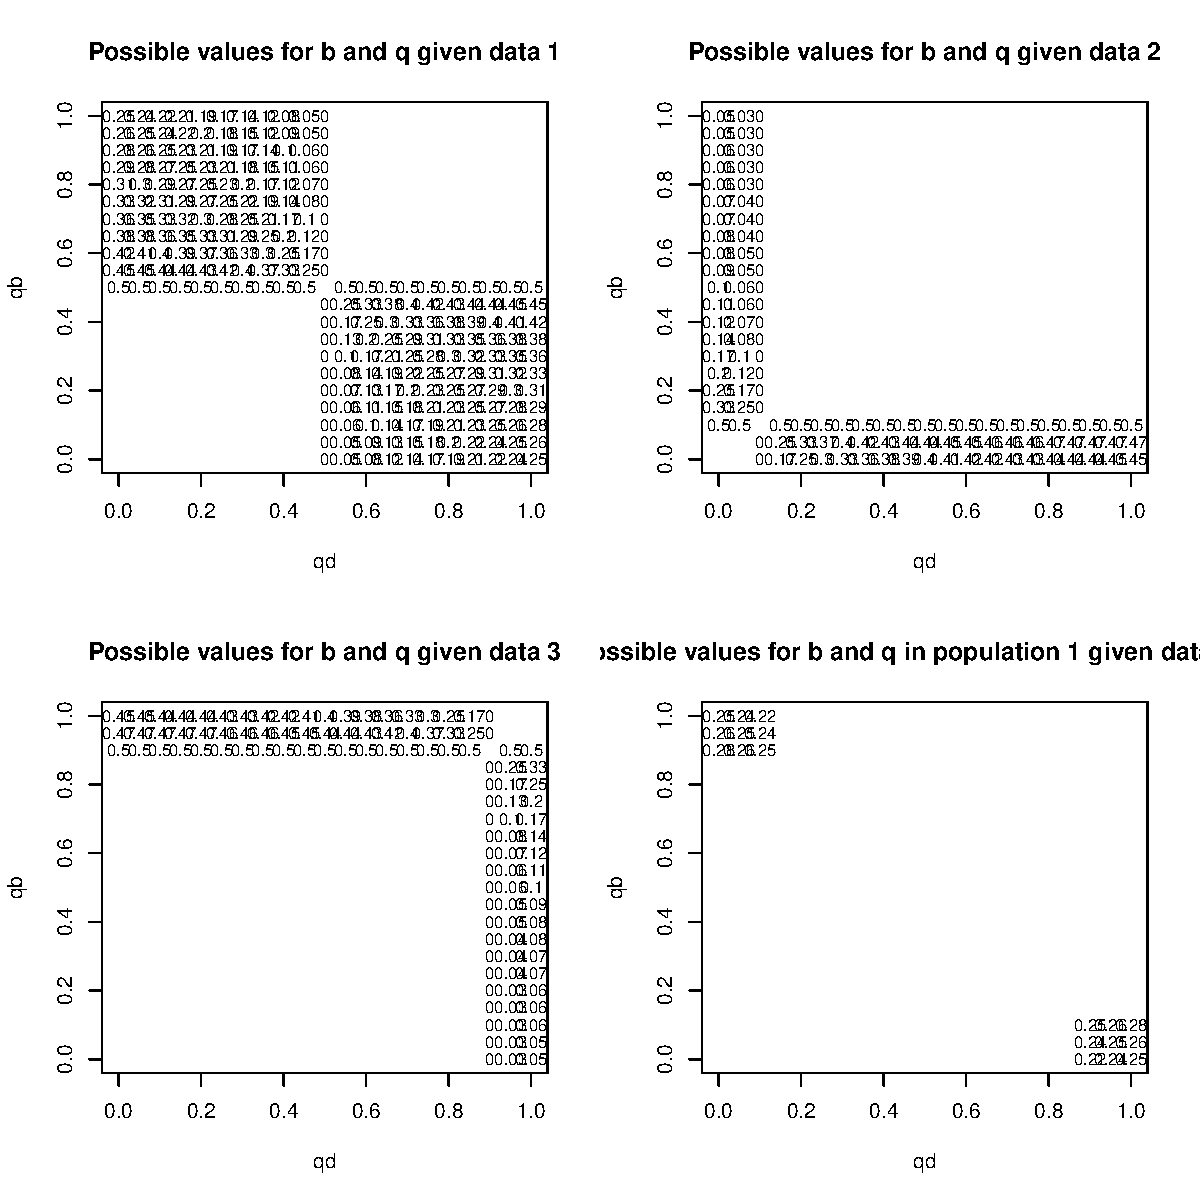
\includegraphics{ii_files/figure-latex/unnamed-chunk-91-1} 

}

\caption{\label{fig:somethingfig} Combinations of $\phi_{b1}$, $\phi_{d1}$ and $b$ values consistent with data from three populations. Populations are assumed to differ in the sizes of groups $A,B,C,D$ but not in the $\phi$ values. Furthermore it is assumed in this illustration that observed data is identical across populations with respect to $X$ and $Y$ but differs with respect to $K$.}\label{fig:unnamed-chunk-91}
\end{figure}

The top left panel of figure \ref{fig:somethingfig} summarizes the learning that is possible from the first population. The axes indicate possible values of \(\phi_{b1}\) and \(\phi_{d1}\); the numbers marked inside the figure are the possible values of \(a\) implied by these values. Note that values are marked only when they collectively satisfy the constraint given in Equation \ref{CC1}.

Key features of the graph are that both \(\phi_{d1}\) and \(\phi_{b1}\) span the whole range between 0 and 1: that is, the constraint does not limit the range of either of these on their own. Second, values of \(b\) range from 0 to 0.5: thus the constraint does not rule out any value for \(b\) not already determined by \(X\), \(Y\) data alone.

However the combinations of possible values are clearly strongly constrained and these combinations depend on the data.

The second and third figures show the analogous set of constraints for two more populations that are identical to the first except that \(K\) is observed in very few of the \(X=Y=1\) cases in the second population and in very many of the \(X=Y=1\) cases in the third. Under the assumption that \(\phi\) is invariant to population, the feasible values of \(\phi\) consists of those values that are admissible in \emph{all} populations. These values are shown in the bottom right figure (they can in fact be identified by considering the intersection of the admissible values from any two of the populations).

From the bottom right figure we learn two things: first, although we have now greatly constrained the set of possible values of \(\phi\), quite distinct values remain possible. Secondly, whatever the true values of \(\phi\) we have in the final figure, we have tightly limited the possible values of \(b\), which we now believe to be approximately 0.25.

The intuition for this result is the following. From population 2 we learn that \(\phi\) cannot be high for both \(b\) and \(d\) types, it must be low for one or the other or both. From population 3 we learn that \(\phi\) cannot be low for both types; it must high for one or the other or both. Together these imply that \(\phi\) must be high for either \(b\) or \(d\) and low for the other. However since in population 1 there is a middling level of \(K\) then there must be a middling frequency of \(b\)s and \(d\)s.

Note finally that in this example, our learning on the level of \(b\) in populations 2 and 3 is less precise: we learn only that \(b\) is either very high or very low, and that it is \emph{not} middling in these populations.

\hypertarget{evaluation}{%
\chapter{Post-estimation: Robustness and Model Evaluation}\label{evaluation}}

\begin{center}\rule{0.5\linewidth}{\linethickness}\end{center}

Model based inference takes the model seriously. But deep down we know that all of these models are wrong, in myriad ways. We examine strategies for figuring out whether a model is likely doing more harm than good.

\begin{center}\rule{0.5\linewidth}{\linethickness}\end{center}

Throughout this book we have maintained the conceit that you believe your model. But it is also obvious that even the most non-parametric seeming models depend on substantive assumptions.

\hypertarget{tools-for-evaluating-models}{%
\section{Tools for evaluating models}\label{tools-for-evaluating-models}}

Check conditional independencies
Check confounding assumptions approach 2 -- say actual confound is q\textasciitilde{}=0; but model assumes q = 0. Draw data from priors, draw data; given data type (001, 100 etc) plot (a) the posterior distribution under no confounding nad (b) the distribution of estimands that gave rise to the data.

Change qual to quant priors in PIMD model

Check restrictions

Check fit

Compare out of sample fit between model

Reality checks -- posterior fits

\hypertarget{evaluating-the-democracy-inequality-model}{%
\section{Evaluating the Democracy-Inequality model}\label{evaluating-the-democracy-inequality-model}}

\hypertarget{prior-check}{%
\section{Prior check}\label{prior-check}}

In a second iteration of the analysis, we show what happens if we loosen the monotonicity restriction on \(I\)'s effect on \(M\). Here we consider negative effects of \(I\) on \(M\) \emph{unlikely}, rather than impossible, and we consider null and positive effects somewhat likely. We refer to these priors as ``quantitative priors'' in the sense that they place a numerical value on beliefs rather than a logical restriction. Here, we set our prior on \(U^M\) as: \(p(U^M=t^M_{10})=0.1\), \(p(U^M=t^M_{00})=0.25\), \(p(U^M=t^M_{11})=0.25\), and \(p(U^M=t^M_{01})=0.4\). We show the results for the inferences given different findings in tables \ref{tab:HK8cases1quant} and \ref{tab:HK8cases2quant}. The mapping into expected posterior variance associated with each strategy is shown by the numbers in parentheses in Table \ref{CaseLearn}.

The results differ in various modest ways. However, the biggest difference we observe is in the degree to which the mobilization clue matters when we are looking for negative effects of inequality. As discussed, if we assumed monotonic positive effects of inequality on mobilization and monotonic positive effects of mobilization on inequality, then the mediator clue is uninformative about the indirect pathway since that pathway can only generate a positive effect. However, if we allow for the possibility of a negative effect of inequality on mobilization, we now make \(M\) informative as a mediator even when the effect of inequality that we are interested in is negative: it is now possible that inequality has a negative effect on democratization via a negative effect on mobilization, followed by a positive effect of mobilization on democratization. So now, observing whether mobilization occurred adds information about whether a negative effect could have occurred via the mobilization pathway.

Moreover, it is possible for the two effects of observing \(M\) on our beliefs to work in opposite ways. What we learn from observing \(M\) about the \(I \rightarrow M \rightarrow D\) pathway may push in a different direction from what we learn from observing \(M\) about the direct \(I \rightarrow D\) pathway. We see this dynamic at work in a case with low inequality and democratization. Where we are only learning about \(M\) as a moderator of \(I\)'s direct effect (monotonicity assumption in place), observing \(M=0\) shifts our beliefs in favor of \(I\)'s negative effect. But where we are learning about \(M\) as both mediator and moderator, observing \(M=0\) shifts our beliefs \emph{against} \(I\)'s negative effect. The reason for this latter result is straightforward: if \(I=0\) and we then see \(M=0\), then we have just learned that inequality's possible indirect negative effect, running via the mobilization pathway, has \emph{not} in fact occurred; and this has a considerable downward effect on our beliefs in an overall negative effect of inequality. This learning outweighs the small positive impact of observing \(M=0\) on our confidence that \(I\) had a direct negative effect on \(D\).

We see these differences most clearly in the cases of Albania (as compared to Mexico) and Nicaragua (as compared to Taiwan). Under priors fully constrained to monotonic causal effects, we saw that the mediator clue, \(M\), made only a small difference to our inferences. However, if we allow for a negative effect of \(I\) on \(M\), even while believing it to be unlikely, observing mobilization in Albania and Nicaragua makes us substantially more confident that inequality mattered, and differentiates our conclusions about these cases more sharply from our conclusions about Mexico and Taiwan, respectively.

\hypertarget{monotonic-restrictions}{%
\section{Monotonic restrictions}\label{monotonic-restrictions}}

Compare fit between model with and without monotonic restrictions

\hypertarget{final-words}{%
\chapter{Final Words}\label{final-words}}

Looking forward to this bit.

\hypertarget{words-of-warning}{%
\section{Words of warning}\label{words-of-warning}}

We started with the story of the engineer and the philosopher.

\hypertarget{part-appendices}{%
\part{Appendices}\label{part-appendices}}

\hypertarget{examplesappendix}{%
\chapter{\texorpdfstring{Analysis of canonical models with \texttt{gbiqq}}{Analysis of canonical models with gbiqq}}\label{examplesappendix}}

\begin{center}\rule{0.5\linewidth}{\linethickness}\end{center}

We walk through a set of canonical models and show how to define and analyze them using \texttt{gbiqq}.

\begin{center}\rule{0.5\linewidth}{\linethickness}\end{center}

\hypertarget{x-causes-y-no-confounding}{%
\section{\texorpdfstring{\(X\) causes \(Y\), no confounding}{X causes Y, no confounding}}\label{x-causes-y-no-confounding}}

In the simplest \(X\) causes \(Y\) model the ATE is identified but the ``probability of causation'' (PC) is not: we can however generally place bounds on PC.

The model can be written:

\begin{Shaded}
\begin{Highlighting}[]
\NormalTok{model <-}\StringTok{ }\KeywordTok{make_model}\NormalTok{(}\StringTok{"X -> Y"}\NormalTok{)}
\KeywordTok{plot_dag}\NormalTok{(model)}
\end{Highlighting}
\end{Shaded}

\includegraphics{ii_files/figure-latex/unnamed-chunk-95-1.pdf}

This sparse definition assumes that there is no confounding and no constraints on the ways \(X\) relates to \(Y\).

You can see the parameter matrix, which confirms this, showing the mapping from parameters to causal types:

\begin{table}[t]

\caption{\label{tab:unnamed-chunk-97}Parameter matrix for X causes Y model without confounding}
\centering
\begin{tabular}{l|r|r|r|r|r|r|r|r}
\hline
  & X0.Y00 & X1.Y00 & X0.Y10 & X1.Y10 & X0.Y01 & X1.Y01 & X0.Y11 & X1.Y11\\
\hline
X0 & 1 & 0 & 1 & 0 & 1 & 0 & 1 & 0\\
\hline
X1 & 0 & 1 & 0 & 1 & 0 & 1 & 0 & 1\\
\hline
Y00 & 1 & 1 & 0 & 0 & 0 & 0 & 0 & 0\\
\hline
Y10 & 0 & 0 & 1 & 1 & 0 & 0 & 0 & 0\\
\hline
Y01 & 0 & 0 & 0 & 0 & 1 & 1 & 0 & 0\\
\hline
Y11 & 0 & 0 & 0 & 0 & 0 & 0 & 1 & 1\\
\hline
\end{tabular}
\end{table}

We can simulate data using the bare bones model and assuming a ``true model'' in which there is a true positive effect of 0.5.

\begin{Shaded}
\begin{Highlighting}[]
\NormalTok{data <-}\StringTok{ }\KeywordTok{simulate_data}\NormalTok{(model, }\DataTypeTok{n =} \DecValTok{1000}\NormalTok{, }
                      \DataTypeTok{parameters =} \KeywordTok{c}\NormalTok{(.}\DecValTok{5}\NormalTok{, }\FloatTok{.5}\NormalTok{, }\FloatTok{.2}\NormalTok{, }\FloatTok{.1}\NormalTok{, }\FloatTok{.6}\NormalTok{, }\FloatTok{.1}\NormalTok{))}
\end{Highlighting}
\end{Shaded}

The kinds of inferences on the probability that \(X\) has a positive effect on \(Y\) given different data is calculated as follows:

\begin{Shaded}
\begin{Highlighting}[]
\NormalTok{updated <-}\StringTok{ }\KeywordTok{gbiqq}\NormalTok{(model, data)}
\end{Highlighting}
\end{Shaded}

We can then ask questions about particular estimands like this:

\begin{Shaded}
\begin{Highlighting}[]
\NormalTok{ATE <-}\StringTok{ "Y[X=1] - Y[X=0]"}
\NormalTok{PC  <-}\StringTok{ "Y[X=1] > Y[X=0]"}

\NormalTok{results <-}\StringTok{ }\NormalTok{gbiqq}\OperatorTok{::}\KeywordTok{get_estimands}\NormalTok{(}
\NormalTok{ updated,}
 \DataTypeTok{queries =} \KeywordTok{list}\NormalTok{(}\DataTypeTok{ATE =}\NormalTok{ ATE, }\DataTypeTok{ATE =}\NormalTok{ ATE, }\DataTypeTok{PC =}\NormalTok{ PC, }\DataTypeTok{PC =}\NormalTok{ PC),}
 \DataTypeTok{using =} \KeywordTok{list}\NormalTok{(}\StringTok{"priors"}\NormalTok{, }\StringTok{"posteriors"}\NormalTok{))}
\end{Highlighting}
\end{Shaded}

\begin{tabular}{l|l|l|r|r}
\hline
Query & Subset & Using & mean & sd\\
\hline
ATE & All & priors & 0.00 & 0.32\\
\hline
ATE & All & posteriors & 0.52 & 0.03\\
\hline
PC & All & priors & 0.25 & 0.20\\
\hline
PC & All & posteriors & 0.61 & 0.06\\
\hline
\end{tabular}

We see from the posterior variance on PC that PC is not identified (or more precisely they key feature is that this distribution does not tighten even with very large N). For more intuition we graph the posteriors:

\includegraphics{ii_files/figure-latex/unnamed-chunk-103-1.pdf}

We find that they do not converge but they do place positive mass in the right range. Within this range, the shape of the posterior depends on the priors only.

\hypertarget{x-causes-y-with-confounding}{%
\section{\texorpdfstring{\(X\) causes \(Y\), with confounding}{X causes Y, with confounding}}\label{x-causes-y-with-confounding}}

An \(X\) causes \(Y\) model with confounding can be written:

\begin{Shaded}
\begin{Highlighting}[]
\NormalTok{model <-}\StringTok{ }\KeywordTok{make_model}\NormalTok{(}\StringTok{"X -> Y"}\NormalTok{) }\OperatorTok
\StringTok{         }\KeywordTok{set_confound}\NormalTok{(}\KeywordTok{list}\NormalTok{(}\DataTypeTok{X =} \StringTok{"(Y[X=1]>Y[X=0])"}\NormalTok{, }\DataTypeTok{X =} \StringTok{"(Y[X=1]<Y[X=0])"}\NormalTok{, }\DataTypeTok{X =} \StringTok{"(Y[X=1] ==1)"}\NormalTok{))}
\KeywordTok{plot_dag}\NormalTok{(model)}
\end{Highlighting}
\end{Shaded}

\includegraphics{ii_files/figure-latex/unnamed-chunk-104-1.pdf}

The parameter matrix here has more parameters than nodal types, reflecting the conditional assignment probabilities of \(X\) -- \(X\) can have different assignment probabilities for different nodal types for \(Y\).

\begin{table}[t]

\caption{\label{tab:unnamed-chunk-106}Parameter matrix for X causes Y model with arbitrary confounding}
\centering
\begin{tabular}{l|r|r|r|r|r|r|r|r}
\hline
  & X0.Y00 & X1.Y00 & X0.Y10 & X1.Y10 & X0.Y01 & X1.Y01 & X0.Y11 & X1.Y11\\
\hline
X0.3 & 0 & 0 & 0 & 0 & 0 & 0 & 1 & 0\\
\hline
X1.3 & 0 & 0 & 0 & 0 & 0 & 0 & 0 & 1\\
\hline
X0.2 & 0 & 0 & 1 & 0 & 0 & 0 & 0 & 0\\
\hline
X1.2 & 0 & 0 & 0 & 1 & 0 & 0 & 0 & 0\\
\hline
X0.1 & 0 & 0 & 0 & 0 & 1 & 0 & 0 & 0\\
\hline
X1.1 & 0 & 0 & 0 & 0 & 0 & 1 & 0 & 0\\
\hline
X0 & 1 & 0 & 0 & 0 & 0 & 0 & 0 & 0\\
\hline
X1 & 0 & 1 & 0 & 0 & 0 & 0 & 0 & 0\\
\hline
Y00 & 1 & 1 & 0 & 0 & 0 & 0 & 0 & 0\\
\hline
Y10 & 0 & 0 & 1 & 1 & 0 & 0 & 0 & 0\\
\hline
Y01 & 0 & 0 & 0 & 0 & 1 & 1 & 0 & 0\\
\hline
Y11 & 0 & 0 & 0 & 0 & 0 & 0 & 1 & 1\\
\hline
\end{tabular}
\end{table}

With the possibility of any type of confounding, the best we can do is place ``Mansky bounds'' on the average causal effect.

To see this, let's plot a histogram of our posterior on average causal effects, given lots of data:

\begin{Shaded}
\begin{Highlighting}[]
\NormalTok{data <-}\StringTok{ }\KeywordTok{simulate_data}\NormalTok{(}
\NormalTok{    model, }\DataTypeTok{n =} \DecValTok{1000}\NormalTok{, }
    \DataTypeTok{parameters =} \KeywordTok{c}\NormalTok{(.}\DecValTok{5}\NormalTok{, }\FloatTok{.5}\NormalTok{, }\FloatTok{.5}\NormalTok{, }\FloatTok{.5}\NormalTok{, }\FloatTok{.5}\NormalTok{, }\FloatTok{.5}\NormalTok{, }\FloatTok{.5}\NormalTok{, }\FloatTok{.5}\NormalTok{, }\FloatTok{.1}\NormalTok{, }\FloatTok{.1}\NormalTok{, }\FloatTok{.7}\NormalTok{, }\FloatTok{.1}\NormalTok{))}
\end{Highlighting}
\end{Shaded}

\begin{Shaded}
\begin{Highlighting}[]
\NormalTok{updated <-}\StringTok{ }\KeywordTok{gbiqq}\NormalTok{(model, data, }\DataTypeTok{refresh =} \DecValTok{0}\NormalTok{)}
\end{Highlighting}
\end{Shaded}

\begin{verbatim}
## Prior distribution added to model
\end{verbatim}

\includegraphics{ii_files/figure-latex/unnamed-chunk-110-1.pdf}

The key thing here is that the posterior on the ATE has shifted, as it should, but it is not tight, even with large data. In fact the distribution of the posterior covers one unit of the range between -1 and 1.

\hypertarget{simple-mediation-model}{%
\section{Simple mediation model}\label{simple-mediation-model}}

We define a simple mediation model and illustrate learning about whether \(X=1\) caused \(Y=1\) from observations of \(M\).

\begin{Shaded}
\begin{Highlighting}[]
\NormalTok{model <-}\StringTok{ }\KeywordTok{make_model}\NormalTok{(}\StringTok{"X -> M -> Y"}\NormalTok{) }\OperatorTok
\StringTok{         }\KeywordTok{set_confound}\NormalTok{(}\DataTypeTok{confound =} \KeywordTok{list}\NormalTok{(}\DataTypeTok{X =} \StringTok{"M[X=1]==1"}\NormalTok{)) }\OperatorTok
\StringTok{         }\KeywordTok{set_parameters}\NormalTok{(}\KeywordTok{c}\NormalTok{(.}\DecValTok{5}\NormalTok{, }\FloatTok{.5}\NormalTok{, }\FloatTok{.2}\NormalTok{, }\FloatTok{.8}\NormalTok{, }
                          \FloatTok{.2}\NormalTok{, }\DecValTok{0}\NormalTok{, }\FloatTok{.8}\NormalTok{, }\DecValTok{0}\NormalTok{, }
                          \FloatTok{.2}\NormalTok{, }\DecValTok{0}\NormalTok{, }\FloatTok{.8}\NormalTok{, }\DecValTok{0}\NormalTok{))}
\end{Highlighting}
\end{Shaded}

\begin{Shaded}
\begin{Highlighting}[]
\KeywordTok{plot_dag}\NormalTok{(model)}
\end{Highlighting}
\end{Shaded}

\includegraphics{ii_files/figure-latex/unnamed-chunk-112-1.pdf}

Data and estimation:

\begin{Shaded}
\begin{Highlighting}[]
\NormalTok{data <-}\StringTok{ }\KeywordTok{simulate_data}\NormalTok{(model, }\DataTypeTok{n =} \DecValTok{1000}\NormalTok{, }\DataTypeTok{using =} \StringTok{"parameters"}\NormalTok{)}
\end{Highlighting}
\end{Shaded}

\begin{Shaded}
\begin{Highlighting}[]
\NormalTok{updated <-}\StringTok{ }\KeywordTok{gbiqq}\NormalTok{(model, data)}
\end{Highlighting}
\end{Shaded}

\begin{Shaded}
\begin{Highlighting}[]
\NormalTok{result <-}\StringTok{ }\NormalTok{gbiqq}\OperatorTok{::}\KeywordTok{get_estimands}\NormalTok{(}
\NormalTok{    updated, }
    \DataTypeTok{queries =} \KeywordTok{list}\NormalTok{(}\DataTypeTok{COE =} \StringTok{"c(Y[X=1] > Y[X=0])"}\NormalTok{), }
    \DataTypeTok{subsets =} \KeywordTok{c}\NormalTok{(}\StringTok{"X==1 & Y==1"}\NormalTok{, }\StringTok{"X==1 & Y==1 & M==0"}\NormalTok{, }\StringTok{"X==1 & Y==1 & M==1"}\NormalTok{),}
    \DataTypeTok{using =} \StringTok{"posteriors"}\NormalTok{)}
\end{Highlighting}
\end{Shaded}

\begin{tabular}{l|l|l|r|r}
\hline
Query & Subset & Using & mean & sd\\
\hline
COE & X==1 \& Y==1 & posteriors & 0.917 & 0.179\\
\hline
COE & X==1 \& Y==1 \& M==0 & posteriors & 0.035 & 0.099\\
\hline
COE & X==1 \& Y==1 \& M==1 & posteriors & 0.918 & 0.179\\
\hline
\end{tabular}

Note that observation of \(M=0\) results in a 0 probability for the posterior that \(X\) caused \(Y\), while observation of \(M=1\) has only a modest positive effect. The mediator thus provides a hoop test for the proposition that \(X\) caused \(Y\).

\hypertarget{simple-moderator-model}{%
\section{Simple moderator model}\label{simple-moderator-model}}

We define a simple model with a moderator and illustrate how updating about COE is possible using the value of a mediator as a clue.

\begin{Shaded}
\begin{Highlighting}[]
\NormalTok{model <-}\StringTok{ }\KeywordTok{make_model}\NormalTok{(}\StringTok{"X -> Y; Z -> Y"}\NormalTok{) }
\KeywordTok{plot_dag}\NormalTok{(model)}
\end{Highlighting}
\end{Shaded}

\includegraphics{ii_files/figure-latex/unnamed-chunk-118-1.pdf}

\begin{Shaded}
\begin{Highlighting}[]
\NormalTok{data <-}\StringTok{ }\KeywordTok{simulate_data}\NormalTok{(}
\NormalTok{    model, }\DataTypeTok{n =} \DecValTok{1000}\NormalTok{, }
    \DataTypeTok{parameters =} \KeywordTok{c}\NormalTok{(.}\DecValTok{5}\NormalTok{, }\FloatTok{.5}\NormalTok{, }\FloatTok{.5}\NormalTok{, }\FloatTok{.5}\NormalTok{, }
                   \FloatTok{.02}\NormalTok{, }\FloatTok{.02}\NormalTok{, }\FloatTok{.02}\NormalTok{, }\FloatTok{.02}\NormalTok{, }\FloatTok{.02}\NormalTok{, }\FloatTok{.02}\NormalTok{, }\FloatTok{.02}\NormalTok{, }\FloatTok{.02}\NormalTok{,}
                   \FloatTok{.02}\NormalTok{, }\FloatTok{.70}\NormalTok{, }\FloatTok{.02}\NormalTok{, }\FloatTok{.02}\NormalTok{, }\FloatTok{.02}\NormalTok{, }\FloatTok{.02}\NormalTok{, }\FloatTok{.02}\NormalTok{, }\FloatTok{.02}\NormalTok{))}
\end{Highlighting}
\end{Shaded}

\begin{Shaded}
\begin{Highlighting}[]
\NormalTok{posterior <-}\StringTok{ }\KeywordTok{gbiqq}\NormalTok{(model, data)}
\end{Highlighting}
\end{Shaded}

\begin{Shaded}
\begin{Highlighting}[]
\NormalTok{result <-}\StringTok{ }\NormalTok{gbiqq}\OperatorTok{::}\KeywordTok{get_estimands}\NormalTok{(}
\NormalTok{    updated, }
    \DataTypeTok{queries =} \KeywordTok{list}\NormalTok{(}\DataTypeTok{COE =} \StringTok{"Y[X=1] > Y[X=0]"}\NormalTok{), }
    \DataTypeTok{subsets =} \KeywordTok{list}\NormalTok{(}\StringTok{"X==1 & Y==1"}\NormalTok{, }\StringTok{"X==1 & Y==1 & Z==0"}\NormalTok{, }\StringTok{"X==1 & Y==1 & Z==1"}\NormalTok{),}
    \DataTypeTok{using =} \StringTok{"posteriors"}\NormalTok{)}
\end{Highlighting}
\end{Shaded}

\begin{tabular}{l|l|l|r|r}
\hline
Query & Subset & Using & mean & sd\\
\hline
COE & X==1 \& Y==1 & posteriors & 0.830 & 0.037\\
\hline
COE & X==1 \& Y==1 \& Z==0 & posteriors & 0.457 & 0.160\\
\hline
COE & X==1 \& Y==1 \& Z==1 & posteriors & 0.898 & 0.029\\
\hline
\end{tabular}

As an exercise, define a model where, learning about a model with moderators allows you to tighten bounds on COE even without observing the value of the mediator.

\hypertarget{an-iv-model}{%
\section{An IV model}\label{an-iv-model}}

We define a simple mediation model and illustrate learning about whether \(X=1\) caused \(Y=1\) from observations of \(M\).

\begin{Shaded}
\begin{Highlighting}[]
\NormalTok{model <-}\StringTok{ }\KeywordTok{make_model}\NormalTok{(}\StringTok{"X -> M -> Y"}\NormalTok{)  }\OperatorTok
\StringTok{         }\KeywordTok{set_confound}\NormalTok{(}\DataTypeTok{confound =} \KeywordTok{list}\NormalTok{(}\DataTypeTok{M =} \StringTok{"Y[M=1]==1"}\NormalTok{)) }

\KeywordTok{plot_dag}\NormalTok{(model)}
\end{Highlighting}
\end{Shaded}

\includegraphics{ii_files/figure-latex/unnamed-chunk-124-1.pdf}

\begin{Shaded}
\begin{Highlighting}[]
\NormalTok{result <-}\StringTok{ }\NormalTok{gbiqq}\OperatorTok{::}\KeywordTok{get_estimands}\NormalTok{(}
\NormalTok{    updated, }
    \DataTypeTok{queries =} \KeywordTok{list}\NormalTok{(}\DataTypeTok{ATE =} \StringTok{"c(Y[M=1] - Y[M=0])"}\NormalTok{), }
    \DataTypeTok{subsets =} \KeywordTok{list}\NormalTok{(}\OtherTok{TRUE}\NormalTok{, }\StringTok{"M[X=1] > M[X=0]"}\NormalTok{,  }\StringTok{"M==0"}\NormalTok{,  }\StringTok{"M==1"}\NormalTok{),}
    \DataTypeTok{using =} \StringTok{"posteriors"}\NormalTok{)}
\end{Highlighting}
\end{Shaded}

\begin{tabular}{l|l|l|r|r}
\hline
Query & Subset & Using & mean & sd\\
\hline
ATE & All & posteriors & 0.591 & 0.050\\
\hline
ATE & M[X=1] > M[X=0] & posteriors & 0.604 & 0.054\\
\hline
ATE & M==0 & posteriors & 0.563 & 0.097\\
\hline
ATE & M==1 & posteriors & 0.619 & 0.033\\
\hline
\end{tabular}

We calculate the average causal effect for all and for the compliers and conditional on values of \(M\).

\hypertarget{a-model-that-allows-application-of-the-frontdoor-criterion}{%
\section{A model that allows application of the frontdoor criterion}\label{a-model-that-allows-application-of-the-frontdoor-criterion}}

\hypertarget{a-model-with-a-violation-of-sequential-ignorability}{%
\section{A model with a violation of sequential ignorability}\label{a-model-with-a-violation-of-sequential-ignorability}}

\hypertarget{learning-from-a-collider}{%
\section{Learning from a collider}\label{learning-from-a-collider}}

Pearl describes a model similar to the following as case for which controlling for covariate \(W\) induces bias in the estimation of the effect of \(X\) on \(Y\), which could otherwise be esimated without bias.

\begin{Shaded}
\begin{Highlighting}[]
\NormalTok{model <-}\StringTok{ }\KeywordTok{make_model}\NormalTok{(}\StringTok{"X -> Y <- S; S -> W"}\NormalTok{) }\OperatorTok
\StringTok{         }\KeywordTok{set_confound}\NormalTok{(}\KeywordTok{list}\NormalTok{(}\DataTypeTok{X =} \StringTok{"W[S=1]==1"}\NormalTok{)) }\OperatorTok
\StringTok{         }\KeywordTok{set_parameters}\NormalTok{(}\KeywordTok{c}\NormalTok{(.}\DecValTok{1}\NormalTok{, }\FloatTok{.9}\NormalTok{, }
                          \FloatTok{.5}\NormalTok{, }\FloatTok{.5}\NormalTok{, }
                          \FloatTok{.9}\NormalTok{, }\FloatTok{.1}\NormalTok{, }
                          \FloatTok{.1}\NormalTok{,.}\DecValTok{1}\NormalTok{,.}\DecValTok{7}\NormalTok{,.}\DecValTok{1}\NormalTok{,}
                          \FloatTok{.2}\NormalTok{, }\DecValTok{0}\NormalTok{,}\DecValTok{0}\NormalTok{,}\DecValTok{0}\NormalTok{, }\DecValTok{0}\NormalTok{,}\DecValTok{0}\NormalTok{,}\DecValTok{0}\NormalTok{,}\DecValTok{0}\NormalTok{, }\FloatTok{.6}\NormalTok{,}\DecValTok{0}\NormalTok{,}\DecValTok{0}\NormalTok{,}\DecValTok{0}\NormalTok{, }\DecValTok{0}\NormalTok{,}\DecValTok{0}\NormalTok{,}\DecValTok{0}\NormalTok{,.}\DecValTok{2}\NormalTok{)) }

\KeywordTok{plot_dag}\NormalTok{(model)}
\end{Highlighting}
\end{Shaded}

\includegraphics{ii_files/figure-latex/unnamed-chunk-129-1.pdf}

\begin{Shaded}
\begin{Highlighting}[]
\NormalTok{data <-}\StringTok{ }\KeywordTok{simulate_data}\NormalTok{(model, }\DataTypeTok{n =}  \DecValTok{20000}\NormalTok{)}
\end{Highlighting}
\end{Shaded}

The true effect of \(X\) on \(Y\) is .3 but the PC is quite different for units with \(W=0\) and W=1\$/

\begin{tabular}{l|l|l|r|r}
\hline
Query & Subset & Using & mean & sd\\
\hline
ATE & All & parameters & 0.300 & NA\\
\hline
ATE & X==1 \& Y==1 & parameters & 0.600 & NA\\
\hline
ATE & X==1 \& Y==1 \& W==0 & parameters & 0.083 & NA\\
\hline
ATE & X==1 \& Y==1 \& W==1 & parameters & 0.725 & NA\\
\hline
\end{tabular}

Priors are:

\begin{tabular}{l|l|l|r|r}
\hline
Query & Subset & Using & mean & sd\\
\hline
ATE & All & priors & 0.003 & 0.140\\
\hline
ATE & X==1 \& Y==1 & priors & 0.502 & 0.137\\
\hline
ATE & X==1 \& Y==1 \& W==0 & priors & 0.503 & 0.142\\
\hline
ATE & X==1 \& Y==1 \& W==1 & priors & 0.501 & 0.141\\
\hline
\end{tabular}

The ATE can be gotten fairly precisely in a simple regression. But controlling for \(W\) introduces bias:

\begin{Shaded}
\begin{Highlighting}[]
\KeywordTok{summary}\NormalTok{(}\KeywordTok{lm}\NormalTok{(Y}\OperatorTok{~}\NormalTok{X, }\DataTypeTok{data =}\NormalTok{ data))}\OperatorTok{$}\NormalTok{coef}
\end{Highlighting}
\end{Shaded}

\begin{verbatim}
##             Estimate Std. Error t value   Pr(>|t|)
## (Intercept)   0.2063   0.006631   31.10 1.794e-207
## X             0.2939   0.007703   38.16 1.246e-307
\end{verbatim}

\begin{Shaded}
\begin{Highlighting}[]
\KeywordTok{summary}\NormalTok{(}\KeywordTok{lm}\NormalTok{(Y}\OperatorTok{~}\NormalTok{X}\OperatorTok{+}\NormalTok{W, }\DataTypeTok{data =}\NormalTok{ data))}\OperatorTok{$}\NormalTok{coef}
\end{Highlighting}
\end{Shaded}

\begin{verbatim}
##             Estimate Std. Error t value   Pr(>|t|)
## (Intercept)  0.07551   0.006521   11.58  6.629e-31
## X            0.21968   0.007229   30.39 2.629e-198
## W            0.37076   0.006333   58.54  0.000e+00
\end{verbatim}

How does the Bayesian model do, with and without data on \(W\)?

Inferences that do not use \(W\) get ATE right on average, but PC is not identified and statements about PC conditional on \(W\) are not possible:

\begin{tabular}{l|l|l|r|r}
\hline
Query & Subset & Using & mean & sd\\
\hline
not named & All & posteriors & 0.290 & 0.007\\
\hline
not named & X==1 \& Y==1 & posteriors & 0.797 & 0.039\\
\hline
not named & X==1 \& Y==1 \& W==0 & posteriors & 0.780 & 0.079\\
\hline
not named & X==1 \& Y==1 \& W==1 & posteriors & 0.778 & 0.079\\
\hline
\end{tabular}

We see including the collider does not induce error in estimation of the ATE, even though it does in a regression framework. It provides an ability to make different PC case level claims given W, but these are nevertheless far off in this example because we still do not have identification.

\begin{tabular}{l|l|l|r|r}
\hline
Query & Subset & Using & mean & sd\\
\hline
not named & All & posteriors & 0.290 & 0.007\\
\hline
not named & X==1 \& Y==1 & posteriors & 0.798 & 0.039\\
\hline
not named & X==1 \& Y==1 \& W==0 & posteriors & 0.594 & 0.133\\
\hline
not named & X==1 \& Y==1 \& W==1 & posteriors & 0.847 & 0.034\\
\hline
\end{tabular}

\hypertarget{a-model-mixing-observational-and-experimental-data}{%
\section{A model mixing observational and experimental data}\label{a-model-mixing-observational-and-experimental-data}}

We imagine that node \(R\) indicates whether a unit was assigned to be randomly assigned to treatment assignment (\(X=Z\) if \(R=1\)) or took on its observational value (\(X=O\) if \(R=0\)). We assume the exclusion restriction that entering the experimental sample is not related to \(Y\) other than through assignment of \(X\).

\begin{Shaded}
\begin{Highlighting}[]
\NormalTok{model <-}\StringTok{ }\KeywordTok{make_model}\NormalTok{(}\StringTok{"R -> X; O ->X; Z -> X; X -> Y"}\NormalTok{) }\OperatorTok
\StringTok{         }\KeywordTok{set_restrictions}\NormalTok{(}\DataTypeTok{causal_type_restrict =} 
                            \StringTok{"X[Z=1, R=1, O=0]!=1 | X[Z=0, R=1, O=0]!=0 | X[Z=1, R=1, O=1]!=1 | X[Z=0, R=1, O=1]!=0 | }
\StringTok{                             X[Z=1, R=0, O=0]!=0 | X[Z=0, R=0, O=0]!=0 | X[Z=1, R=0, O=1]!=1 | X[Z=0, R=0, O=1]!=1"}\NormalTok{) }\OperatorTok
\StringTok{         }\KeywordTok{set_confound}\NormalTok{(}\KeywordTok{list}\NormalTok{(}\DataTypeTok{O =} \StringTok{"(Y[X=1]>Y[X=0])"}\NormalTok{, }\DataTypeTok{O =} \StringTok{"(Y[X=1]<Y[X=0])"}\NormalTok{, }\DataTypeTok{O =} \StringTok{"(Y[X=1] ==1)"}\NormalTok{))}

\KeywordTok{plot_dag}\NormalTok{(model)}
\end{Highlighting}
\end{Shaded}

\includegraphics{ii_files/figure-latex/unnamed-chunk-138-1.pdf}

The parameter matrix has just one type for \(X\) since \(X\) really operates here as a kind of switch, inheriting the value of \(Z\) or \(O\) depending on \(R\). Parameters allow for complete confounding between \(O\) and \(Y\) by \(Z\) and \(Y\) are unconfounded.

\begin{Shaded}
\begin{Highlighting}[]
\NormalTok{model <-}\StringTok{ }\KeywordTok{set_parameters}\NormalTok{(model, }\KeywordTok{c}\NormalTok{(.}\DecValTok{2}\NormalTok{, }\FloatTok{.8}\NormalTok{, }
                                 \FloatTok{.8}\NormalTok{, }\FloatTok{.2}\NormalTok{, }
                                 \FloatTok{.2}\NormalTok{, }\FloatTok{.8}\NormalTok{, }
                                 \FloatTok{.8}\NormalTok{, }\FloatTok{.2}\NormalTok{, }
                                 \FloatTok{.5}\NormalTok{, }\FloatTok{.5}\NormalTok{, }
                                 \FloatTok{.5}\NormalTok{, }\FloatTok{.5}\NormalTok{, }
                                 \DecValTok{1}\NormalTok{,}
                                 \FloatTok{.2}\NormalTok{, }\FloatTok{.2}\NormalTok{, }\FloatTok{.4}\NormalTok{, }\FloatTok{.2}\NormalTok{))}
\end{Highlighting}
\end{Shaded}

The estimands:

\begin{tabular}{l|l|l|r|r}
\hline
Query & Subset & Using & mean & sd\\
\hline
ATE & All & parameters & 0.2 & NA\\
\hline
ATE & R==0 & parameters & 0.2 & NA\\
\hline
ATE & R==1 & parameters & 0.2 & NA\\
\hline
\end{tabular}

The priors:

\begin{tabular}{l|l|l|r|r}
\hline
Query & Subset & Using & mean & sd\\
\hline
ATE & All & priors & -0.003 & 0.363\\
\hline
ATE & R==0 & priors & -0.003 & 0.363\\
\hline
ATE & R==1 & priors & -0.003 & 0.363\\
\hline
\end{tabular}

Data:

\begin{Shaded}
\begin{Highlighting}[]
\NormalTok{data <-}\StringTok{ }\KeywordTok{simulate_data}\NormalTok{(model, }\DataTypeTok{n =} \DecValTok{600}\NormalTok{)}

\CommentTok{# Uncomment if data on $O$ is not available for cases assigned to $R=1$.}
\CommentTok{# data$O[data$R == 1] <- NA   }
\end{Highlighting}
\end{Shaded}

The true effect is .2 but naive analysis on the observational data would yield a srtongly upwardly biased estimate.

The gbiqq estimates are:

\begin{Shaded}
\begin{Highlighting}[]
\NormalTok{posterior <-}\StringTok{ }\KeywordTok{gbiqq}\NormalTok{(model, data)}
\end{Highlighting}
\end{Shaded}

\begin{tabular}{l|l|l|r|r}
\hline
Query & Subset & Using & mean & sd\\
\hline
ATE & All & posteriors & 0.208 & 0.044\\
\hline
ATE & R==0 & posteriors & 0.208 & 0.044\\
\hline
ATE & R==1 & posteriors & 0.208 & 0.044\\
\hline
\end{tabular}

Did observational data improve the estimates from the experimental data?

\begin{Shaded}
\begin{Highlighting}[]
\NormalTok{posterior <-}\StringTok{ }\KeywordTok{gbiqq}\NormalTok{(model, data[data}\OperatorTok{$}\NormalTok{R}\OperatorTok{==}\DecValTok{1}\NormalTok{,])}
\end{Highlighting}
\end{Shaded}

\begin{tabular}{l|l|l|r|r}
\hline
Query & Subset & Using & mean & sd\\
\hline
ATE & All & posteriors & 0.166 & 0.056\\
\hline
ATE & R==0 & posteriors & 0.166 & 0.056\\
\hline
ATE & R==1 & posteriors & 0.166 & 0.056\\
\hline
\end{tabular}

A key quantity of interest from this model is the average effect of treatment conditional on being in treatment in the observational group. We have:

\begin{tabular}{l|l|l|r|r}
\hline
Query & Subset & Using & mean & sd\\
\hline
ATE & R==1 \& X==0 & posteriors & 0.166 & 0.056\\
\hline
ATE & R==1 \& X==1 & posteriors & 0.166 & 0.056\\
\hline
ATE & R==0 \& X==0 & posteriors & -0.101 & 0.083\\
\hline
ATE & R==0 \& X==1 & posteriors & 0.362 & 0.071\\
\hline
\end{tabular}

\hypertarget{transportation-of-findings-across-contexts}{%
\section{Transportation of findings across contexts}\label{transportation-of-findings-across-contexts}}

We study the effect of \(X\) on \(Y\) in country 1 and want to make inferences to country 2, Our problem however is that countries differ in terms of some feature, \(W\), that is distributed differently in the two countries and that affects \(Y\) via some mechanism \(K\).

{[}{[}We assume that we have an experiment in country 1 but only observational variation in country 2.{]}{]}

For instance, \(X\) is cash and \(Y\) is welfare. \(W\) is background levels of conflict which affects welfare via security \(K\), possibly differently in both countries.

Although they differ, we have the following encompassing theory for both countries.

\begin{Shaded}
\begin{Highlighting}[]
\NormalTok{model <-}\StringTok{ }\KeywordTok{make_model}\NormalTok{(}\StringTok{"W -> K -> Y <- X"}\NormalTok{)}
\end{Highlighting}
\end{Shaded}

\includegraphics{ii_files/figure-latex/unnamed-chunk-152-1.pdf}

\bibliography{bib.bib,packages.bib}


\end{document}
